\documentclass[a4paper,11pt,openany, twoside,fleqn]{book}
%\IfFileExists{cmap.sty}{%
%  \usepackage[resetfonts]{cmap}
%}{} % makes pdfs searchable and copyable
\usepackage{geometry}
\usepackage{phd}

%\usepackage[utf8]{inputenc}
% Redefine the LaTeX commands that are replaced by textcomp.
% This was swiped right out of ltoutenc.dtx, but with "\text..."
% changed to "\ltext...".
\DeclareTextCommandDefault{\ltextcopyright}{\textcircled{c}}
\DeclareTextCommandDefault{\ltextregistered}{\textcircled{\scshape r}}
\DeclareTextCommandDefault{\ltexttrademark}{\textsuperscript{TM}}
\DeclareTextCommandDefault{\ltextordfeminine}{\textsuperscript{a}}
\DeclareTextCommandDefault{\ltextordmasculine}{\textsuperscript{o}}
\usepackage{latexsym}						% additional latex symbols

%------------------------------------- FONT UTILITIES --------------------------------------
\usepackage{scalefnt}						% utility for scaling fonts
\usepackage{fonttable}						% utility for font tables
%% Save a symbol that we know is going to get redefined.
%% code is from the Comprehensive Latex symbol list
%\newcommand*{\savesymbol}[1]{%
%  \expandafter\let\csname orig#1\expandafter\endcsname\csname#1\endcsname
%  \expandafter\let\csname #1\endcsname\relax
%}
%%
% Restore a previously saved symbol, and rename the current one.
%\newcommand*{\restoresymbol}[2]{%
%  \expandafter\global\expandafter\let\csname#1#2\expandafter\endcsname%
%    \csname#2\endcsname
%  \expandafter\global\expandafter\let\csname#2\expandafter\endcsname%
%    \csname orig#2\endcsname}

% Rename a robust command.
%\newcommand*{\renamerobustsymbol}[2]{%
%  \expandafter\let\expandafter\origrealcommand
%    \csname #2\space\endcsname
%  \expandafter\global\expandafter\let\csname#1#2\endcsname=\origrealcommand
%}

%% Test if a symbol is not saved.
%\makeatletter
%\def\ifnotsavedsym@helper#1#2!{\expandafter\ifx\csname orig#2\endcsname\relax}
%\newcommand*{\ifnotsavedsym}[1]{%
%  \expandafter\ifnotsavedsym@helper\string#1!%
%}
%\makeatother


%% VARIOUS TYPESETTING MACROS AND BABEL
\usepackage[top=1.5cm, left=2cm,bottom=2.5cm,right=1.5cm,showframe=false]{geometry}[2002/07/08] % showframe is off

\usepackage[ngerman,german,polutonikogreek,greek,latin,english]{babel}
%\usepackage{teubner}
\usepackage{pdftexcmds} % For \pdf@strcmp

%% ----------------  --  POSITIONING AND LAYOUT/BOXES/RULES ---------------
%\usepackage{chngpage}                                             % provides adjustwidth gives errors


\usepackage[absolute,overlay]{textpos}
\usepackage{boxedminipage}					% used for fancy boxes
\usepackage{shapepar}                                              % for shaping paragraphs
%\let\cutout\undefined
%\let\endcutout\undefined						% to use with cutwin easier
%\usepackage{cutwin}
\usepackage{addlines}                                               % enlargethis page
\usepackage{framed}                                                % For frames

%% Tables
%%  TABLES




%% --------------------------- TYPOGRAPHY -------------------------------------------
%\usepackage{microtype}					% for better spacing and less hyphens

%\IfFileExists{mathpazo.sty}{\RequirePackage[osf,sc]{mathpazo}}{}
%\IfFileExists{helvet.sty}{\RequirePackage[scaled=0.90]{helvet}}{}
%\IfFileExists{beramono.sty}{\RequirePackage[scaled=0.85]{beramono}}{}

%\usepackage{pacioli}


\IfFileExists{yfonts.sty}
{\usepackage{yfonts}[2003/01/08]} 				% fraktur font (titlepage only, in examples)
{\providecommand{\textgoth}[1]{\textbf{##1}}}		% fallback if no yfonts



%-------------------------- MATHS -------------------------------------------------
% MATHEMATICS


\let\equation\gather                           %% See tabu and hyperref docs
\let\endequation\endgather




\usepackage{multienum} 					% used in maths chapter


%\usepackage{teubner}					% for additional greek fonts and commands
%\usepackage{teubner-subset}				% try to minimize conflicts
%% ------------------------  GRAPHICS PACKAGES -----------------------------------
%\usepackage{graphicx}					% for including graphics
%\usepackage{wrapfig}				% wrapped figures and subfigures
%\usepackage[grid=false,subgridcolor=green!20,	% grid used only in draft mode
%                   gridcolor=gray!80, texcoord=true, 
%                   gridunit=cm]{eso-pic}
%\usepackage{rotating}					% for rotated figures and text
%\usepackage{tikz} 
%
%\usepackage[figurename=Figure.,]{caption}

%---------------------------------------- FOR MACRO UTILITIES ---------------------
%
\usepackage{changepage}    % checks if page is odd or not
\strictpagecheck
\usepackage{keyval}
\RequirePackage{ifmtarg}
\RequirePackage{fp}
\RequirePackage{ifthen}
\RequirePackage{xstring}

%
%%------------------------ Specific to this project --------------------------------------
%%%
%%  internal package for cover pages
%% Verbatims
% The fancyvrb package lets us customize the formatting of verbatim
% environments.  We use a slightly smaller font.



%\usepackage{morelogos}						% define logos to work with
%										% lower case saves keystrokes
\makeatletter
\long\def\imghangleft#1#2{%
     \figure
     \leftskip-1.6cm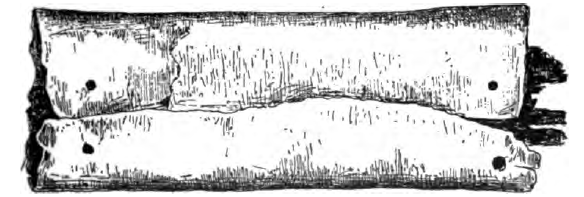
\includegraphics[scale=1.1]{./graphics/copper-sheath}\par
     \centerline{\textsc{Copper Sheath}}
    \endfigure
}
%	Graphics
%	Graphics are handled at many levels. Firstly when an item is added to the database
% 	an image is added. This can be retrieved with |\getstampfield{#1}{#2}{image}|.
%	
%
%% The graphic command simply sets up the correct paths and includes the
%% image, this might need to be left in a box for later usage
%% I will come back and change it later.
%% KEY DEFINITIONS
\usepackage{xkeyval}
\define@key{img}{width}[1cm]{\def\img@width{#1}}
\define@key{img}{height}{\def\img@height{#1}}
\define@key{img}{offsetx}{\def\img@offsetx{#1}}
\define@key{img}{offsety}{\def\img@offsety{#1}}
\define@key{img}{border}{\def\img@border{#1}}
\define@key{img}{padding}{\def\img@padding{#1}}
\define@key{img}{style}{\def\img@style{#1}}
\define@key{img}{bottommargin}{\def\img@bottommargin{#1}}
\define@key{img}{keepaspectratio}{\def\img@keepaspectratio{keepaspectratio}}
\define@key{imgpg}{pagestyle}{\def\imgpg@pagestyle{#1}}
%% Set defaults for all keys
\setkeys{img}{offsetx=0pt, offsety=0pt,width=3cm, keepaspectratio=keepaspectratio,
                      border=0pt, padding=0pt,bottommargin=0pt}
%% Create the command graphic

%%% We create a new command to place images 
%\newcommand\putimage[2][0pt]{%
%%% Set the keys
%%\setkeys{img}{#1}%
%%\setlength\fboxrule\img@border%
%%\setlength\fboxsep\img@padding%
%%\ifdim\img@offsety=0pt% 
%%\else%
%%\vspace*{\img@offsety}%
%%\fi%
%%%\hskip\img@offsetx%
%%\setlength{\tempa}{\img@width}
%\fboxsep=0pt
%\fboxrule=0pt
%\protect\def\setcaption{\captionof{figure}{This is the caption for the figure\lorem}}%
%\begin{minipage}{\linewidth}%
%\includegraphics[width=\linewidth]{./graphics/#2}%
%\end{minipage}
%}%\vspace*{\img@bottommargin}}%

%

\DeclareRobustCommand{\putcaption}[1]{\setcaption}


%%
% An environment for paragraph-style section
% borrowed from the Tufte-LaTeX class
\providecommand\newthought[1]{%
   \addvspace{1.0\baselineskip plus 0.5ex minus 0.2ex}%
   \noindent\textsc{#1}%
}

\let\allcaps\textsc
\let\sidenotesize\small
\def\isempty{}
\makeatother


\newcounter{wrapwidth}
\newcount \Zw
\newcount \Zh
% text flowed image - file name, width, height pixels, vertical offset (normally -24, -12 for top of page)
\newcommand\pngright[4]{
\Zw=#2 \divide \Zw by 10
\Zh=#3 \divide \Zh by 120  \advance\Zh by 1
\setcounter{wrapwidth}{\Zw}
\begin{wrapfigure}[\Zh]{r}{\value{wrapwidth}pt}
\begin{center}
\vspace{#4pt}
\includegraphics*[width=\Zw pt]{images/#1}
\end{center}
\end{wrapfigure}}

% text flowed image scaling * #4 / #5 (never occurs at top of page)
\newcommand\pngrightsc[5]{
\Zw=#2 \multiply \Zw by #4 \divide \Zw by #5
\Zh=#3 \multiply \Zh by #4 \divide \Zh by #5
\pngright{#1}{\Zw}{\Zh}{-24}}

% centred image - file name, width, height pixels (height is comment only, easier for developer to change to & from flowed)
\newcommand\pngcent[3]{
\Zw=#2 \divide \Zw by 10
\begin{center}
\includegraphics*[width=\Zw pt]{images/#1}
\end{center}}


% italic text in maths with spacing
\newcommand\opit[1]{\operatorname{\textit{#1}}}

% small text in maths
\newcommand\smallinmath[1]{{\scriptstyle #1}}
%\newcommand\decimals[1]{,{\!}{\scriptstyle #1}}
%
%% Header with conditional page skip
\newcommand\condpagelarge[1]{
\vspace{\baselineskip}
\Needspace*{4\baselineskip}\begin{center}{\large #1}\end{center}}

%% Proposition with page
\newcommand\forcepageprop[1]{
\newpage
\begin{center}{\large #1}\end{center}}
%
%% Proposition without page
\newcommand\propnopage[1]{
\begin{center}{\large #1}\end{center}}
%
%
%% Section with page
\newcommand\sectpage[1]{
\vspace{\baselineskip}\hrule\newpage\hrule\vspace{\baselineskip}
\begin{center}{\LARGE \gesperrt{SECT}{6}.\hspace{12pt}#1}\end{center}}
%
%% Section without page
\newcommand\sectnopage[1]{
\begin{center}{\LARGE \gesperrt{SECT}{6}.\hspace{12pt}#1}\end{center}}
%
%
%%\ggesperrt#1 }
%
\usepackage{layout}
%
%
%%% Some lengths used in calculations rather use temlength
%\global\newlength\imagewidth
%
\makeatletter
%Returns a single digit hexadecimal number (0{9, A{F) from
%given hnumber i, which must either be a numeric register or
%a number ending with a space! from the kernel
% we add the space, works only up to 16
%\newcounter{cnt}
%\setcounter{cnt}{0}
%\loop
% \ifnum\thecnt<20
%   \stepcounter{cnt}
%   \thecnt\  \tohex{\thecnt}\\
%\repeat
%\def\tohex#1{\hexnumber@{#1 }}
%\makeatother

% Hyphenate some awkward words
\hyphenation{Figure Table %to avoid it hyphenating and hyperref crossing page boundary
Hero-do-tus equi-noxes dig-its-first-block}

\def\hlred{ }
\def\image#1#2#3#4\par{%
    %\leavevmode\par
    \parindent10pt
    \setlength{\intextsep}{0pt} % top and bottom sizing
    \setlength{\columnsep}{10pt}
   \begin{wrapfigure}{#1}[0pt]{#2} % specify width only
    %\fbox
   \end{wrapfigure}
#4\par}
%
%
%% shortcut for wrapped images
\def\wrappedimage#1#2#3#4\par{%
%\leavevmode\par
\parindent10pt
\setlength{\intextsep}{0pt} % top and bottom sizing
\setlength{\columnsep}{10pt}% separators at side
\begin{wrapfigure}{#1}[0pt]{#2} % specify width only
%\fbox
\end{wrapfigure}
#4\par}
%
%% Presentation command in Foreward styling.
\newcommand{\AtRight}[2][\parindent]{%
  \leavevmode\par
  \hbox to\linewidth{\hss\textbf{#2}\hskip#1}
}


%\usepackage[bookmarks=true]{hyperref}
%\hypersetup{%
%    bookmarks=false,    % show bookmarks bar?
%    pdftitle={TeX and friends hackers manual},    % title
%    pdfauthor={Yiannis Lazarides},                     % author
%    pdfsubject={TeX and LaTeX},                        % subject of the document
%    pdfkeywords={TeX, LaTeX, graphics, images}, % list of keywords
%    colorlinks=true,       % false: boxed links; true: colored links
%    linkcolor=blue,       % color of internal links
%    citecolor=black,       % color of links to bibliography
%    filecolor=black,        % color of file links
%    urlcolor=purple,        % color of external links
%    linktoc=page            % only page is linked
%}
%\usepackage{subfig}
%%%%%%%%%%%%%%%  Doccommands %%%%%%%%%%

\def\person#1{#1}

\let\sidenote\footnote
\let\marginnote\footnote
%%% GOOD QUESTION
%%% enables <#1> to be inserted automatically
\newfont\yltt{ectt1000}

\newenvironment{docs}{%
}{}
%%\catcode`\<=\active
%%\gdef<##1>{\ensuremath{\langle\mbox{\textsl{##1}}\rangle}}


\makeatletter
%\usepackage{doccommands}
%\usepackage{setlistings}


% Set up the epigraph to be a bit wider
\setlength{\epigraphwidth}{0.4\textwidth} 
\setlength{\epigraphrule}{0pt}

\newenvironment{marginfigure}{}{}
\newenvironment{fullwidth}{}{}
\makeindex

\makeatletter

\newenvironment{adjustmargins}[2]{%
  \begin{list}{}{%
    \topsep\z@%
    \listparindent\parindent%
    \parsep\parskip%
   \@ifmtarg{#1}{\setlength{\leftmargin}{\z@}}%
   {\setlength{\leftmargin}{#1}}%
   \@ifmtarg{#2}{\setlength{\rightmargin}{\z@}}%
   {\setlength{\rightmargin}{#2}}%
}
\item[]}{\end{list}}

 \newenvironment{adjustmargins*}[2]{%
 \begin{list}{}{%
 \topsep\z@%
 \listparindent\parindent%
 \parsep\parskip%
 \checkoddpage
 \ifoddpage % odd numbered page
 \@ifmtarg{#1}{\setlength{\leftmargin}{\z@}}%
 {\setlength{\leftmargin}{#1}}%
 \@ifmtarg{#2}{\setlength{\rightmargin}{\z@}}%
 {\setlength{\rightmargin}{#2}}%
 \else % even numbered page
 \@ifmtarg{#2}{\setlength{\leftmargin}{\z@}}%
 {\setlength{\leftmargin}{#2}}%
 \@ifmtarg{#1}{\setlength{\rightmargin}{\z@}}%
 {\setlength{\rightmargin}{#1}}%
\fi
}
\item[]}{\end{list}}

%  The case study environment

%     define a placeholder for the label. This enables babel to translate it.
%     #1 short label for case study 
\makeatletter
\gdef\thecasestudylabel{Case Study}
\newenvironment{casestudy}[2][]{%
    \addcontentsline{toc}{section}{\thecasestudylabel:  #1}
    %phantomsection
   \clearpage % clears a page if necessary
    \topline
   {\noindent\large CASE STUDY\par}\vspace{3.5pt}
   \noindent\textsc{\large#1}\par
   \bigskip
   {#2}
   \medskip
   \topline
}{%
\vfill\bottomline}


\makeatother
 %Use Donald Arseneau's improved float parameters.
%% FLOAT SET-UP
%% 

\makeatletter
  \def\K@opt@arg[#1]#2{\incsyms\indexcommand[#1]{#2}#1 &\ttfamily\string#2}
  \def\K@no@opt@arg#1{\incsyms\indexcommand[#1]{#1}#1 &\ttfamily\string#1}
  \def\K{\@ifnextchar[{\K@opt@arg}{\K@no@opt@arg}}
\makeatother


\def\smallcaps#1s{}
\def\allcaps#1{}
\def\people#1{}
\usepackage{wasysym}
% Ancient languages
%\usepackage{rotunda}
%\usepackage{huncial}
%\usepackage{uncial}
%\usepackage{runic}
%\usepackage{pifont}
%\usepackage{phoenician}
%\usepackage{cypriot}
%\usepackage{hieroglf}
% Syllabaries
\newcommand{\UC}{A B C D E F G H I J K L M N O P Q R S T U V W X Y Z}
\newcommand{\LC}{a b c d e f g h i j k l m n o p q r s t u v w x y z}
\newcommand{\SY}{+ ? / |}
\newcommand{\ST}{\Hms\ \Hibp\ \Hibw\ \Hibs\ \Hibl\ \Hsv\ 
                 \Hman\ \Htongue\ \Hscribe\ \Hplural\ \Hdual}
\newcommand{\SN}{\Hone\ \Hten\ \Hhundred\ \Hthousand\ \HXthousand
                 \HCthousand\ \Hmillion}
\newcommand{\Caesar}{\pmvglyph{\Hk:\Hy:\HS:\Hl:\HS}}
% This is for chess 
\usepackage[LSBC1,LSBC2,LSBC4,TS1,OT1,T1]{fontenc}		%this needs checking out
\usepackage{textcomp, mathcomp}
\usepackage[skaknew]{chessboard,skak}
\usepackage{latexsym}
\usepackage{textcomp, mathcomp}
\font\logo=logo10
\font\sknf=SkakNew-Figurine
\font\sknfbx=SkakNew-FigurineBold
\font\skndia=SkakNew-DiagramT
%
%
%%% The arabtex package screws up with footnote!!!!
%\usepackage{arabtex}
%%
%% We want to use the package ecclesiatic, this appears to give us problems with catcodes for :
%%% Gives problem with @for took out, does not safely in combination with other packages, play
%%% nice
%%\usepackage{ecclesiastic}
\usepackage{ellipsis} % better ldots, must be loaded last

%% properties ala lisp
\def\csn#1{\csname#1\endcsname}%
\long\def\ece#1#2{\expandafter#1\csname#2\endcsname}%
% ATOM PROPERTY VALUE  FROM EPLAIN
\long\def\setproperty#1#2#3{\ece\edef{#1@p#2}{#3}}%
\long\def\setpropertyglobal#1#2#3{\ece\xdef{#1@p#2}{#3}}%

\long\def\getproperty#1#2{%
  \expandafter\ifx\csname#1@p#2\endcsname\relax
  % then \end{multicols}{2}pty
  \else \csname#1@p#2\endcsname
  \fi
}%
%% Command factory for example
%% not needed in package
\gdef\commandfactory#1#2{%
   \global\expandafter\def\csname#1\endcsname{#1}
   \global\expandafter\def\csname#1caption\endcsname{#2}
}

%% Knuths smile box from 
%\centerline{\bf Stable Husbands}
%\bigskip
%\centerline{\sl Donald E. Knuth, Rajeev Motwani, and Boris Pittel}
%\centerline{\sl  Computer Science Department, Stanford University}
\def\pfbox % new experimental version (DEK, November 88)
{{\ooalign{\hfil\lower.06ex % a smiley face
 \hbox{$\scriptscriptstyle\frown$}\hfil\crcr
 \hfil\lower.7ex\hbox{\"{}}\hfil\crcr
 \mathhexbox20D}}}

\def\hangleft{}

%\usepackage{fp}
% \section{Guidelines for images}
%  You need to crop your images carefully so there is no white space around the frame. MAny an hour
% can get lost thinking that an image is too large, whereas the offset is just white border on the image.
%% Define full page environments for starting pages etc....
%% Note that both \newgeometry and \restoregeometry insert \clearpage where they are called
%\newlength{\miniwidth}{0pt}


%% Headings and captions
%% The oneline caption is a caption that is below the image
%% at a tight space. If it is almost the length of the width of the image
%% it is stretched to fit the whole line

 
%
%
%%% Define the oneline caption
%\newcommand\onelinecaption[2][]{%
%    \par\tinyskip
%    \setlength\offsetfromright{0em}%
%    \bgroup%
%        %\vskip0pt plus1pt minus1pt %
%        \reset@font
%        \sffamily
%        \bfseries%
%        \footnotesize%
%        \hfill\hfill#2\hbox to \offsetfromright{}%
%     \egroup%
%}

%% Define the oneline centered caption. This has to become a key 
%% command if possible, first one to use pgf/key system?
%% #1 offset from top
%% add to table of contents etc
%\newcommand\onelinecaptioncentered[2][]{%
%   \vskip0pt\vspace*{#1}
%    \setlength\offsetfromright{0em}%
%    \bgroup%
%        %\vskip0pt plus1pt minus1pt %
%        \reset@font
%        \sffamily
%        \bfseries%
%        \footnotesize%
%        \hfill#2\hbox to \offsetfromright{}\hfill%
%     \egroup%
%}





\begin{filecontents}{kroll.sty}
%% 
%% 
%% We define some more skips 
%% tinyskip is 4pt skip to have the captions tights below images
\def\tinyskip{\vskip 4pt plus 1pt minus 1pt}
%
%% By-line command
\newcommand\byline[2][]{\footnotesize \textbf{#1}#2}%

%% \onelineheader is a header that must fit on line
%    We define a new if to check if the header must be centered
%    this is set true by default
\newif\if@centeredheader
\@centeredheadertrue
%
%   Provide an author command to set the
%   font for the header
\gdef\setonelineheaderfont#1{%
  \gdef\onelineheaderfont{#1}%
}
%   Set default font
\setonelineheaderfont{\sffamily\LARGE\bf}
%    onelineheader
%% #1 c,l,r provides for the heading justification
%% set default as centered
\newcommand\onelineheader[2][c]{%
\leavevmode\par
 \if#1c\@centeredheadertrue
  \else\@centeredheaderfalse
\fi
 \vspace{1.5\baselineskip}%
   \if@centeredheader 
      \bgroup\onelineheaderfont\centering\mbox{#2}\par\egroup 
   \else
      \if#1r% flushright
         \bgroup\hfill\hfill\onelineheaderfont\mbox{#2}\par\egroup 
       \else
          \bgroup\onelineheaderfont\mbox{#2}\par\egroup 
      \fi
   \fi%
   \vspace{0.5\baselineskip}%
}

%\renewcommand\LARGE{\@setfontsize\LARGE\@xviipt{12}}
\newcommand\HeadFont{\@setfontsize\HeadFont{30}{35}}

 \newcommand\MainHeader[1]{{\leavevmode\par \begin{center}\HeadFont #1 \end{center}
\vspace{1cm}}}

\newcommand\MainHeadera[1]{{\leavevmode\par\centering \HeadFont #1\par\vspace{1cm}}}

%\newlength{\miniwidthii}{0pt}
\def\starttemplate#1{%
    \overfullrule0pt
   \fboxsep=0pt
   \fboxrule=0pt
    \thispagestyle{plain}
   \gdef\Geometry{%
   \newgeometry{top=10mm,inner=1cm,outer=1cm,bottom=20mm,marginparsep=0pt,marginparwidth=0pt}}
   \ifthenelse{\equal{kroll01}{kroll01}}{%
      \Geometry
%% we now calculate some of the parameters
%% required
    \setlength\miniwidthi{0.3\textwidth}%
    \setlength\miniwidthii{0.67\textwidth}%
    \setlength\sepmainhorizontal{0.03\textwidth}%
    % The caption text at the bottom image
    % not happy with this name, need to change it.
   % \newcommand\byline[2][]{\footnotesize \textbf{##1}##2}%
   %
%% Create environments for convenience
    \renewenvironment{leftcolumn}[1]{%
        \begin{minipage}[b]{\miniwidthi} ##1}{\end{minipage}\hspace{1.5em}}%
    \renewenvironment{rightcolumn}[1]{%
        \begin{minipage}[b]{\miniwidthii} ##1}{\end{minipage}}%
%% Create right column environment
 }{}%end ifthenelse
\def\stoptemplate{\restoregeometry}
}
%  to be removed in file version
%  only for compatibility with some older
%  examples
\let\aheader\byline
\end{filecontents}
\usepackage{kroll}

\def\Paragraph#1{\par\noindent \textbf{#1}\hspace{1em}}

%\newcommand\end{multicols}{2}phasis[2][red]{\lstset{emph={write,void,writeln,#2},
%   emphstyle={\ttfamily\textcolor{#1}}}}%


\usepackage{fancyvrb}
\fvset{fontsize=\normalsize}
\DefineShortVerb{\|}
\usepackage{lipsum,xcolor, listings, multicol,etoolbox}

\usepackage{bibentry}
\usepackage{setlistings}


\RequirePackage[scaled=0.85]{berasans}
\RequirePackage[scaled=0.85]{beramono}


%\renewcommand{\ttdefault}{ectt1000}			% prefer old tt font


%%
\usepackage{pgfplots}
\usepackage{pgfpl
stable}
\pgfplotsset{compat=newest}
\usepackage{datetime}
\usepackage{datenumber}
\usepackage{pgfmanual}
\usepackage[listings,theorems]{tcolorbox}
\begin{document}

%
%\Alphabet
%
%\frogking
%
%\dogs
%
%\fox
%
%\onepar






\listoftables


\overfullrule0pt

\restoregeometry

\frontmatter
\setlength\columnsep{2.03em}


% This is the cover page
\thispagestyle{empty}
\coverpage{./graphics/cockfight}{Y. Lazarides}{Published by Camel Press}
\secondpage
\tableofcontents
%\listoffigures  still giving problems

%%%% MAIN TEXT
\pagestyle{headings}
\mainmatter


\clearpage

\clearpage
\newgeometry{left=0in,right=0in}
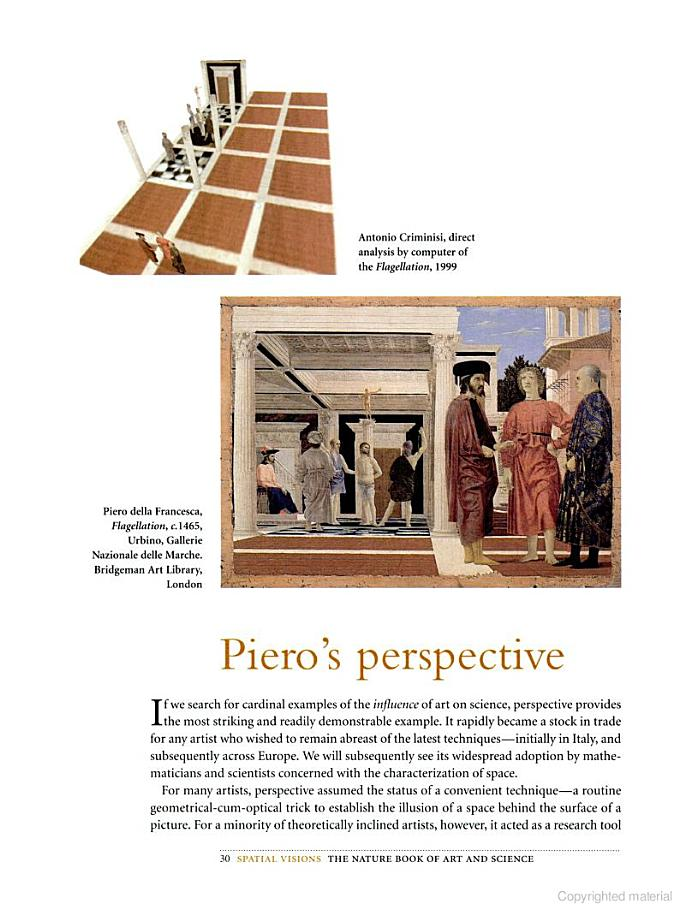
\includegraphics{./graphics/piero}


\includegraphics{./graphics/vision}



\restoregeometry


\newgeometry{left=1in,right=1in}
{\LARGE{\textbf{AN UNUSUAL OPENING}}}

\topline
\begin{multicols}{2}
\captionof{figure}{Bill Bryson's book  \textit{The lost continent: travels in small-town America} has an unusual first paragraph opening it has the equivalent of long equal sign, followed by the first three words in small caps, but without the capital letter being higher than the rest of the letters. }

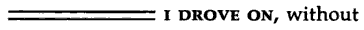
\includegraphics[width=0.32\textwidth]{./graphics/droveon}

\columnbreak
\fbox{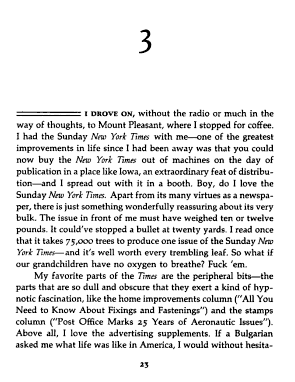
\includegraphics[width=\linewidth]{./graphics/billbryson02}}
\end{multicols}
\bottomline


\newcommand{\lettrinerule}[1]{%
  \settoheight{\dimen0}{\scshape #1}%
  \noindent
  \vbox to \dimen0{\hrule width 5em height1.5pt\vfill\hrule height1.5pt}\kern.5em
  \textsc{#1}}

%@book{bryson1989lost,
%  title={The lost continent: travels in small-town America},
%  author={Bryson, B.},
%  isbn={9780060161583},
%  lccn={89045027},
%  url={http://books.google.com.qa/books?id=2Uk-UnvvUEcC},
%  year={1989},
%  publisher={Harper \& Row}
%}

\lettrine{A}{n unusual opening} for a first paragraph can be found in Bill Bryson's best seller  \textit{The lost continent: travels in small-town America}. This is not very difficult to reproduce using 

\begin{quote}
\large

\lettrinerule I DROVE ON, without the radio or much in the way of thoughts, to Mount Pleasant, where I stopped for coffee. I had the Sunday \textit{New York Times} with me---one of the greatest improvements in life since I had been away was that you could now buy the \textit{New York Times} out of machines on the day of publication
\end{quote}

\restoregeometry

\let\citep\cite
\let\citet\cite
\let\citeauthor\cite
\let\docpkg\cmd
\let\doccmd\cmd
\let\sourceatright\relax
\let\graybox\relax
\let\setmalay\relax
\let\ArabTeX\relax
\let\bibtex\relax
\def\ctan{ctan.org}
\input{preamble}  % the preamble

\restoregeometry
\part{MATHEMATICS}
%\chapter{Typesetting Mathematics}
%\epigraph{Perhaps some day a typesetting language will become standardized to the 
%point where papers can be submitted to the American Mathematical Society 
%from computer to computer via telephone lines. Galley proofs will not be 
%necessary, but referees  and / or copy editors could send suggested changes to 
%the author, and he could insert these into the manuscript, again via telephone. }{Donald Knuth, 1979}
%
%%\renewcommand\figurename{\bf Fig.\thinspace }
%%\begin{marginfigure}%
%%\captionsetup[marginfigure]{margin=10pt,font=small,labelfont=bf}%
%%  \hskip -10pt\relax\includegraphics[width=1.5\linewidth]{./graphics/maths1}
%%  \captionof{figure}{Bookcases in the library of the University of Leiden: from a print by J.C. Woudanus, dated 1610. (Lent by the Syndics of the University Press.)}
%%  \label{fig:marginfig1}
%%\end{marginfigure}
%
%Most people discover, \alltex when they are faced with the production of a thesis or paper that includes lots of
%mathematical text. It is the rais\`on detrait for \tex. In this chapter we will discuss the typesetting of mathematics, common pitfalls and solutions. We will also review some typographical questions.
%
%You can start writing mathematical text, without any additional loading of packages, either in plain \tex or \latex. The reality is that most institutions have developed their own styles and common packages used by AMS have found widespread use. We will discussing these extensively, but first let us look at how to enter mathematical text. To enter mathematical text in plain \tex you just use the |\$|\ldots|\$| for inline math and |\$\$|\ldots|\$\$| for displayed math.
%% Example template kroll01


\chapter{maths}

\parindent1em

\starttemplate{kroll}
\thispagestyle{empty}
    \begin{leftcolumn}
       %\MainHeader{Leon\\[15pt] Kroll}
      {{\centering \huge  THE ART OF \\
       TYPESETTING\\
       MATHS\\}}
      \medskip
       {\justifying \small Perhaps some day a typesetting language will become standardized to the 
point where papers can be submitted to the American Mathematical Society 
from computer to computer via telephone lines. Galley proofs will not be 
necessary, but referees  and / or copy editors could send suggested changes to 
the author, and he could insert these into the manuscript, again via telephone.\par
\hfill \textit{Donald Knuth}}
\medskip
       \putimage[width=1.0\linewidth]{halmos}\par
       \aheader{shows Kroll at 59. Says he. ``Painting is fascinating'' even when motif my own mug.}
   \end{leftcolumn}
   \begin{rightcolumn}
       \putimage[width=\linewidth]{themathematician}
       \onelinecaption{{\resizebox{\linewidth}{5.5pt}{\bfseries The Mathematician (1918) an oil painting by the Mexican artist Diego Rivera. }}\par}

     \vspace*{1.5\baselineskip}

  \centerline{\onelineheader{TYPESETTING MATHEMATICS}}
      \begin{multicols}{2}
      \small
      \lettrine{M}{ost people} discover, \alltex when they are faced with the production of a thesis or paper that includes lots of
mathematical text. It is the rais\`on detrait for \tex. In this chapter we will discuss the typesetting of mathematics, common pitfalls and solutions. We will also review some typographical questions.
\parindent1em

You can start writing mathematical text, without any additional loading of packages, either in plain \tex or \latex. The reality is that most institutions have developed their own styles and common packages used by AMS have found widespread use. We will discussing these extensively, but first let us look at how to enter mathematical text. 

To enter mathematical text in plain \tex you just use the |$|\ldots|$| for inline math and |$$|\ldots|$$| for displayed math. We now illustrate, the usage with and example.
      \end{multicols}
   \end{rightcolumn}
\stoptemplate


\newgeometry{left=2.5cm,right=2.5cm}
\pagestyle{headings}
\definecolor{shadecolor}{rgb}{0.9,0.9,0.9}

\section{Inline and Display Math}
Mathematical typesetting involves either inline math formulae, which are part of a paragraph of text or display math which are a block of mathematical material. \tex will typeset inline math by enclosing the material between 
\$...\$. 
\bigskip

\begin{tcblisting}{colback=blue!5,boxrule=2pt,colframe=blue!75!black,title=\textbf{TeX style inline and display math},width=0.75\textwidth}
This is an inline equation $a^2+b^2=c^2$

And this equation is a display equation:
$$a^2+b^2=c^2$$
\end{tcblisting}
\bigskip

The above code, is valid in \latex and its variants as well. However in certain cases, especially for displayed math, this can introduce some blank lines. Lamport redefined
the \$\$. For inline math use |\(...\)| and for display math |\[...\] |. The above example can be written as:
\bigskip

\begin{tcblisting}{colback=blue!5,boxrule=2pt,colframe=blue!75!black,title=Basic Definitions,width=0.75\textwidth}
This is an inline equation \(a^2+b^2=c^2\)

And this equation is a display equation:
\[a^2+b^2=c^2\]

\begin{math}
\sum_{i=1}^{n}i=\frac{1}{2}n\cdot(n+1)
\end{math}
\end{tcblisting}
\bigskip


As you can observe the output remains the same.  Spaces within  maths environment are ignored, so use this to your advantage when writing maths. As mentioned earlier, we can use |\[...\]| for display math.

We can now try a rather longer example, before getting into more details:
\begin{shaded}
\begin{teXXX}
\[ \sum a_1+a_2+\dots a_n \]
\end{teXXX}
\[ \sum a_1+a_2+\dots a_n \]
\end{shaded}

\section{Displayed Equations}
Displayed equations, can either be displayed \emph{flushed left} or \emph{centered}, depending on the option loaded with the standard classes, for example in article use

\begin{teX}
\documentclass[imperial,11pt,openany, twoside,fleqn]{octavo}[2005/09/16]
\end{teX}

We will see, how to change the formatting a bit later on.

\section{Greek letters}

Mathematicians and Engineers, quickly run out of symbols to use with their equations and hence use Greek letters. All
the Greek letters are available in \tex{} 

\begin{table}[htbp]
\centering
\begin{tabular}{llllllll}
\toprule
$\alpha$  &\doccmd{alpha} &$\beta$ &\doccmd{beta} &$\gamma$ &\doccmd{gamma} &$\delta$ &\doccmd{delta}\\
$\epsilon$  &\doccmd{epsilon} &$\varepsilon$ &\doccmd{varepsilon} &$\zeta$ &\doccmd{zeta} &$\eta$ &\doccmd{eta}\\
\bottomrule
\end{tabular}
\end{table}



Sometimes accents are put above or below symbols. The control words used for accents
in mathematics are different from those used for normal text. The normal text control words
may not be used for mathematics and vice-versa.\sidenote{\texbook 135-136 }. See also
\href{mathmode.pdf}{http://www.tex.ac.uk/tex-archive/info/math/voss/mathmode/Mathmode.pdf}

\section{Fractions}

There are two ways of typesetting a fraction in \tex{}: it can be typeset as $1/4$ or in the form $\frac{1}{4}$. The first case is entered with no special control characters that is,  \verb+ $1/2$+. The second case is just entered with the control word \cmd{over}.  Hence\verb+ ${1} \over {4}$+ gives ${1} \over {4}$. \LaTeX\ provides a macro \cmd{frac}.

A more complex example,

\begin{teX}
\[
a+\gamma \over \delta^2
\]
\end{teX}

\[a+\gamma \over \delta^2\]

One complication with using maths in-line with text is that of using different type of fonts. There is a very useful and interesting discussion in the package \pkg{xfrac}. 

 One of the first exercises in \emph{The \TeX Book} is to design a
 macro for split level fractions. The solution presented is fairly
  simple, using a \emph{virgule} (a slash) for separating the two
  components. It looks okay because the text font and math font of
  Computer Modern look almost identical.\index{virgule}

  The proper symbol to use instead of the virgule is a \emph{solidus}\sidenote{The solidus (/) \index{solidus} is a punctuation mark used to indicate fractions including fractional currency. It may also be called a shilling mark, an in-line fraction bar, or a fraction slash. Its Unicode encoding is \texttt{U+2044}.

The solidus is similar to another punctuation mark, the slash, which is found on standard keyboards; the slash is closer to being vertical than the solidus. These are two distinct symbols that traditionally have entirely different uses. However, many people no longer distinguish between them, and when there is no alternative it is acceptable to use the slash in place of the solidus.
Both the ISO and Unicode designate the solidus as \texttt{FRACTION SLASH U+2044} and the slash as \texttt{SOLIDUS U+002F}. This contradicts long-established English typesetting terminology (See Bringhurst.}
  which does not exist in Computer Modern. It is however available in
  the European Computer Modern fonts, but I'll get back to that.

  The most common way to produce split level fractions within \LaTeX\
  is by means of the \docpkg{nicefrac} package. Part of the reason it
  has found widespread use is due to the strange design of the
  built-in text fractions of the EC fonts, which look like this:
  \textonehalf. The package is very simple to use but there are a few
  issues:

 \begin{itemize}
  \item It uses the virgule instead of the solidus.
  \item Font size of numerator and denominator is bigger than in the
    built-in symbol. Compare Palatino: \switch{ppl}{\nicefrac{1}{2}}
    vs. \switch{ppl}{\textonehalf }. (\sfrac{1}{2})

  \item It doesn't correct for fonts using text figures such as in the
    \docpkg{eco} package. Compare \switch{cmor}{\nicefrac{1}{2}} and
    \switch{cmor}{\nicefrac{8}{9}}.
  \item In math mode, it doesn't always pick up the correct math
    alphabet.
 \end{itemize}
 In short: \docpkg{nicefrac} doesn't attempt to be the answer to
 everything and so this is not a criticism of the package. It works
 quite well for Computer Modern which was pretty much what was widely
 available at the time it was developed. Users these days, however,
 have a choice of many fonts when they write their documents.

With |xfrac| we can switch fonts easily

 ``You take \sfrac[cmr2]{1}{2} cup of sugar, \ldots''




\section{Square roots}

The square root sign, which historically derived from a dot is now simply typeset a square root it is only necessary to use the construction \cmd{sqrt}. Hence

\begin{teX}
$\sqrt{x^2+y^2}$
\end{teX}

will give $\sqrt{x^2+y^2}$


Notice that \tex takes care of the placement of
symbols and the height and length of the radical. To make cube or other roots, the control
words \cmd{root} and \cmd{of} are used. You get $\root n \of {1+x^n}$ from the input 

\begin{teX}
   $\root n \of  {1+x^n}$ 
\end{teX}

A possible alternative is to use the control word \cmd{surd}; the input \verb+ $\surd 2$+ will
produce $\surd 2$.

When typesetting square roots care should be taken, to use struts appropriately to get the sizing right.

\section{Trigonometric and other Functions}
There are several types of functions that appear frequently in mathematical text. In
an equation like $\sin2x+\cos2x=1$ the trigonometric functions \cmd{sin} and \cmd{cos} are in
roman rather than italic type. This is the usual mathematical convention to indicate that
it is a function being described and not the product of three variables. The control words
\doccmd{sin} and \doccmd{cos} will use the right typeface automatically. Here is a table of these and some
other special functions:

\begin{teX}
\sin \cos \tan \cot \sec \csc \arcsin \arccos
\arctan \sinh \cosh \tanh \coth \lim \sup \inf
\limsup \liminf \log \ln \lg \exp \det \deg
\dim \hom \ker \max \min \arg \gcd \Pr
\end{teX}

\begin{tcblisting}{colback=blue!5,boxrule=2pt,colframe=blue!75!black,title=\textbf{TeX style inline and display math},width=0.75\textwidth}
\[ \cos(2\theta) = 2 \cos^{2}2 \theta-1\]
\end{tcblisting}

Functions that are missing from a basic instllation can be either defined or one can use one of the many packages that supplement the above.

\clearpage

\section{Using special symbols}

Special symbols such as dingbats loaded using the |pifont| package need to be encloded within an |\mbox| in order to be able to display the glyph properly.
\bigskip

\begin{tcblisting}{colback=blue!5,boxrule=2pt,colframe=blue!75!black,title=\textbf{DINGBATS},width=0.9\textwidth}
\label{e14}
 We start by showing that the function $f(x)=x^2$ is
continuous over the set $X_2$\label{p:X2} defined as the interval
$[0,1]$ where numerals $\frac{i}{\mbox{\ding{172}}}, 0 \le i \le
\mbox{\ding{172}},$ are used to express its points in units $\mu$.
First of all, note that the set $X_2$ is continuous in   $\mu$
because its points are equidistant with the distance
$d=\mbox{\ding{172}}^{-1}$. Since this function is strictly
increasing,  to show its continuity it is sufficient to check the
difference $f(x)-f(x^{-})$ at the point $x=1$. In this case,
$x^{-}=1-\mbox{\ding{172}}^{-1}$ and we have
\[
 f(1)-f(1-\mbox{\ding{172}}^{-1})=
 1-(1-\mbox{\ding{172}}^{-1})^2 =
 2\mbox{\ding{172}}^{-1}(-1)\mbox{\ding{172}}^{-2}.
\]
This number is infinitesimal, thus $f(x)=x^2$ is continuous over
the set $X_2$. \hfill $\Box$
\end{tcblisting}
\bigskip

\cs{Box}
Notice the use of the |\Box| command to draw a square for  end of proof symbol. This is from the amsmath package. The box is placed at the end of the line using |\hfill $\Box$|.



\section{Partial derivatives}

Partial derivatives can be typeset using the \latex{} command \cmd{partial}
\begin{teXX}
\[
 \sqrt{\frac{x^2}{k+1}}\qquad
  x^\frac{2}{k+1}\qquad
  \frac{\partial^2f}
  {\partial x^2}
\]
\end{teXX}




\begin{equation*}
\sqrt{\frac{x^2}{k+1}}\qquad
x^\frac{2}{k+1}\qquad
\frac{\partial^2f}
{\partial x^2}
\end{equation*}


\newthought{Binomial Coefficients}

To typeset binomial coefficients or similar structures, use the command
\cmd{binom} from \docpkg{amsmath}:\index{amsmath!binom}

Pascal's rule can be typeset as:

\begin{shaded}
\begin{teXX}
\[
\binom{n}{k} =\binom{n-1}{k}
+ \binom{n-1}{k-1}
\]
\end{teXX}
\[
\binom{n}{k} =\binom{n-1}{k}
+ \binom{n-1}{k-1}
\]
\end{shaded}

\clearpage




\section{Matrices}

\begin{equation*}
\mathbf{X} = \left(
\begin{array}{ccc}
x_1 & x_2 & \ldots \\
x_3 & x_4 & \ldots \\
\vdots & \vdots & \ddots
\end{array} \right)
\end{equation*}

\begin{equation*}
\begin{matrix}
1 & 2 \\
3 & 4
\end{matrix} \qquad
\begin{bmatrix}
p_{11} & p_{12} & \ldots
& p_{1n} \\
p_{21} & p_{22} & \ldots
& p_{2n} \\
\vdots & \vdots & \ddots
& \vdots \\
p_{m1} & p_{m2} & \ldots
& p_{mn}
\end{bmatrix}
\end{equation*}


\subsection{vmatrix}
\begin{gather*}
\begin{vmatrix}
aa' + bb' + cc' & ea' + fb' + gc' \\
ae' + bf' + cg' & ee' + ff' + gg'
\end{vmatrix} \\
%
{} = \begin{vmatrix}
a & b \\
e & f
\end{vmatrix}  \begin{vmatrix}
a' & b' \\
e' & f'
\end{vmatrix} + \begin{vmatrix}
a & c \\
e & g
\end{vmatrix}  \begin{vmatrix}
a' & c' \\
e' & g'
\end{vmatrix} + \begin{vmatrix}
b & c \\
f & g
\end{vmatrix}  \begin{vmatrix}
b' & c' \\
f' & g'
\end{vmatrix}.
\end{gather*}


\section{Displayed equations}
All of the mathematics covered so far has identical input whether it is to be typeset
in-line or displayed. At this point we’ll look at some situations that apply to displayed
equations only.





\section{Single equations that are too long}

In many cases equations need to be written over two or more lines. The \docpkg{amsmath} package, provides an environment that is suitable for this:

\emphasis{cos}
\begin{teXXX}
\begin{multline}
   a + b + c + d + e + f+ g + h + i  + k + l + m + n + o + p\\
              = j + k + l + m + n +\cos^{2}-1
\end{multline}
\end{teXXX}

\begin{multline}
a + b + c + d + e + f+ g + h + i  + k + l + m + n + o + p\\
= j + k + l + m + n +\cos^{2}-1
\end{multline}

\newpage
\section{array environment}
This is simply the same as the eqnarray environment only with the possibility of
variable rows and columns and the fact, that the whole formula has only one
equation number and that the array environment can only be part of another math
environment, like the equation environment or the displaymath environment. With
@{} before the first and after the last column the additional space |\arraycolsep| is
not used, which maybe important when using left aligned equations.

\begin{tcblisting}{colback=blue!5,boxrule=2pt,colframe=blue!75!black,title=\textbf{The egnarray Environment},width=1.05\textwidth}
\begin{eqnarray}
a & = & b + c \\
& = & d + e + f + g + h + i
+ j + k + l \nonumber \\
&& +\: m + n + o \\
& = & p + q + r + s
\end{eqnarray}
\end{tcblisting}



the equations
to be aligned are entered with each one terminated by \doccmd{cr}. In each equation there should be
one alignment symbol \& to indicate where the alignment should take place. This is usually
done at the equal signs, although it is not necessary to do so. For example

\verb*+ \qquad( )+ produce

\begin{tcblisting}{colback=blue!5,boxrule=2pt,colframe=blue!75!black,title=\textbf{The array Environment},width=1.05\textwidth}
Thus to change $\frac34$ to a decimal divide $4$ into $3$
and we get $.75$ as a result, thus:
\[
\begin{array}{r@{}r@{}}
4 \; & \vline \; 3.00 \\\cline{2-2}
     &            .75
\end{array}
\]

To find the square root of a four-figure number
such as our example calls for, work it out in the
following manner:
\[
\arraycolsep=0em
\begin{array}{cccccccccccc}
\multicolumn{3}{c}{\text{2d pair}} &\qquad&\qquad&
\multicolumn{3}{c}{\text{1st pair}}&\qquad&\qquad&
\multicolumn{2}{c}{\text{square root}}\\
 & \overbrace{\quad}&\ZZZ&&&\ZZZ&\overbrace{\quad}&\ZZZ\\
 & 42 &&&&& 25 &&&&\vline\;65&(answer)\\\cline{11-11}
 & 36 &&&&& \\\cline{2-2}
\multirow{2}{*}{125\:} & \vline\hfill \Z6 \hfill&&&&& 25\\
 & \vline\hfill \Z6 \hfill&&&&& 25\\\cline{2-7}
\end{array}
\]

\end{tcblisting}

\subsection{Array environment in game theory}
This example is from \footnote{From determinacy to Nash equilibrium,St\'ephane Le Roux, TU Darmstadt }
\begin{tcblisting}{colback=blue!5,boxrule=2pt,colframe=blue!75!black,title=\textbf{The array Environment},width=1.05\textwidth}
The game $\langle\{a,b,c\},\{1,2,3,4\}^3,\{0,1,2,3,4\},v,(<_d)_{d\in\{a,b,c\}}\rangle$ is represented below, where player $a$ chooses the row, $b$ the column, and $c$ the array. 
\[\begin{array}{c@{\hspace{1cm}}c@{\hspace{1cm}}c@{\hspace{1cm}}c}
\begin{array}{|c|c|c|c|}
\hline 1 & 1 & 1 & 1\\
\hline 1 & 1 & 1 & 1\\
\hline 1 & 1 & 1 & 1\\
\hline 4 & 1 & 1 & 1\\
\hline
\end{array}
&
\begin{array}{|c|c|c|c|}
\hline 1 & 2 & 1 & 1\\
\hline 2 & 2 & 2 & 2\\
\hline 1 & 2 & 1 & 1\\
\hline 4 & 2 & 1 & 1\\
\hline
\end{array}
&
\begin{array}{|c|c|c|c|}
\hline 1 & 1 & 3 & 1\\
\hline 1 & 1 & 3 & 1\\
\hline 3 & 3 & 3 & 3\\
\hline 4 & 1 & 3 & 1\\
\hline
\end{array}
&
\begin{array}{|c|c|c|c|}
\hline 2 & 4 & 4 & 4\\
\hline 4 & 3 & 4 & 4\\
\hline 4 & 4 & 4 & 4\\
\hline 0 & 0 & 0 & 0\\
\hline
\end{array}
\end{array}
\]
Let us show that the game $\langle\{a,b,c\},\{1,\dots,n\}^3,\{0,\dots,n\},v,(<_d)_{d\in\{a,b,c\}}\rangle$ witnesses the claim. First, the preferences are linear orders indeed. Second, let us show that there is no Nash equilibrium by case-splitting below. 
\end{tcblisting}

\section{The AMSmath Package}

The amsmath package offers four different align environments, align, alignat, falign, xalignat and xxalignat. In difference to the eqnarray environment from standard LATEX the ``three'' parts of one equation expr.-symbol-expr. are divided by only one
ampersand in two parts. In general the ampersand should be before the symbol
to get the right spacing, e.g., y \&= x. 

\subsection{The align environment}

The align environment is an improvement over \latex's eqnarray environment. It is very similar to a tabular
environment and is aligned at the |&|.

\begin{tcblisting}{colback=blue!5,boxrule=2pt,colframe=blue!75!black,title=\textbf{The Align Environment},width=1.05\textwidth}
\begin{align}
         y & =d\label{eq:IntoSection}\\
         y & =cx+d\\
 y_{12} & =bx^{2}+cx+d\\
     y(x) & =ax^{3}+bx^{2}+cx+d
 \end{align}

\begin{align*}
\therefore (13 - x_1) + (13 - x_2) + \dotsb + (13 - x_p) + r &= 52\,,\\
\therefore 13p - (x_1 + x_2 + \dotsb + x_p) + r              &= 52\,,\\
\therefore x_1 + x_2 + \dotsb + x_p                          &= 13p - 52 + r\\
                                                          &= 13 (p - 4) + r\,.
\end{align*}

whence we conclude that $\gamma$ is a primitive root modulo $p$. But
\begin{align*}
\gamma^{p-1}-1 &=
     g^{p-1} - 1 + \frac{p-1}{1!}g^{p-2}xp +
        \frac{(p-1)(p-2)}{2!}g^{p-3}x^2p^2 + \ldots \\
  &= p\left(kp + \frac{p-1}{1!}g^{p-2}x +
        \frac{(p-1)(p-2)}{2!}g^{p-3}x^2p + \ldots\right).
\end{align*}
\end{tcblisting}

\subsection{The aligned environment}
The aligned environment allows more than one horizontal alignment but has only one equation number.
\newcommand{\dotsb}{\ldots}			% use lower dots after +-
\newcommand{\dotsbsmall}{\ldot\!\ldot\!\ldot}
\newcommand{\ldot}{\mathbin{.}}			% dot with math spacing
\newcommand{\nobf}[1]{\no \textbf{#1}}		% \no with bold number
\begin{tcblisting}{colback=blue!5,boxrule=2pt,colframe=blue!75!black,title=\textbf{The \texttt{aligned} Environment},width=1.05\textwidth}
\begin{equation}
\begin{aligned}
 &\:C_1x^{r_1}\,[\varphi_{r_1 0} \,+ \varphi_{r_1 1}\log x \,+ \dotsb + \varphi_{r_1 \alpha_1}(\log x)^{\alpha_1}]\\
+&\:C_2x^{r_2}\,[\varphi_{r_2 0} \,+ \varphi_{r_2 1}\log x \,+ \dotsb + \varphi_{r_2 \alpha_2}(\log x)^{\alpha_2}]\\
+&\multispan{1}{\:\dotfill}\\
+&\:C_nx^{r_n}[\varphi_{r_n 0} + \varphi_{r_n 1}\log x + \dotsb + \varphi_{r_n \alpha_n}(\log x)^{\alpha_n}],
\end{aligned}
\end{equation}

\[
\tag{98}
\left\{\qquad
\begin{aligned}
T_1 &= T_2 = T_3 (=T)\\
p_1 &= p_2 = p_3\\
s_1-s_2 &= \frac{(u_1-u_2)+p_1(v_1-v_2)}{T}\\
s_2-s_3 &= \frac{(u_2-u_3)+p_2(v_2-v_3)}{T}.
\end{aligned}
\right.
\]
\end{tcblisting}

\subsection{Interrupting a display}

In many instances you will want to interrupt a display with some text, you can use |\intertext|.

\begin{tcblisting}{colback=blue!5,boxrule=2pt,colframe=blue!75!black,title=\texttt{intertext},width=1.05\textwidth}
\begin{align}
U &= M u = M(c_v T + b)\\
S &= M(c_v  \log T + \frac{R}{m}  \log v + a),\\
\intertext{and}
F &= M \left\{T(c_v - a - c_v \log T) - \frac{RT}{m} \log v + b \right\}.
\end{align}
\end{tcblisting}

The command intertext can onl come after a |\\| or |\\| command. Its function is to preserve the alignment after the text is typeset. This is a common reuirement in many mathematical structures and the command is available in all of amsmath aligning environments.






\subsection{The alignat environment}
The alignat environment means \emph{align at} and can be used to align a set of equations vertically at more than one place.



\begin{tcblisting}{colback=blue!5,boxrule=2pt,colframe=blue!75!black,title=\textbf{alignat},width=1.05\textwidth}
\renewcommand{\dotsb}{\ldots}			% use lower dots after +-
\renewcommand{\dotsbsmall}{\ldot\!\ldot\!\ldot}
\renewcommand{\ldot}{\mathbin{.}}			% dot with math spacing
\renewcommand{\nobf}[1]{\no \textbf{#1}}	

\begin{alignat*}{5}
  &p_{i+1}\dfrac{d^{m-i-1}y_1}{dx^{m-i-1}} &&+ \dotsbsmall +p_{m}y_1
  && = -\Big(\dfrac{d^{m}y_1}{dx^{m}} &&+p_1\dfrac{d^{m-1}y_1}{dx^{m-1}}
  &&+ \dotsbsmall +p_{i}\dfrac{d^{m-i}y_1}{dx^{m-i}}\Big), \\
\multispan{10}{\makebox[36em]{\dotfill},}\\
 &p_{i+1}\dfrac{d^{m-i-1}y_{m-i}}{dx^{m-i-1}} &&+ \dotsbsmall +p_{m}y_{m-i}\!
 &&= -\Big(\dfrac{d^{m}y_{m-i}}{dx^{m}} &&+ p_1\dfrac{d^{m-1}y_{m-i}}{dx^{m-1}}
 &&+ \dotsbsmall +p_{i}\dfrac{d^{m-i}y_{m-i}}{dx^{m-i}}\Big).
\end{alignat*}
\end{tcblisting}



When using one of the align environments, there should be no |\\| at the end of the
last line, otherwise you’ll get another equation number for this ``empty''  line


\clearpage
\subsection{Multline}
The |multline| environment is another attempt at displaying long equations. It will set the first line flush left and the last one flush right. It can be quite useful when one has very long equations. The line break is marked with |\\|. It is good typographical practice to have the first line shorter thn the last line and not the other way around.

\begin{tcblisting}{colback=blue!5,boxrule=2pt,colframe=blue!75!black,title=\textbf{Multline},width=1.05\textwidth}
Example unumbered
\begin{multline*}
x^{\rho}f(x, \rho) = x^{\rho} \Big [ u_{m}x^{m}\frac{\rho(\rho-1)\ldots (\rho-m+1)}{x^{m}} \\
                   + u_{m-1}x^{m-1}\frac{\rho(\rho-1)\ldots (\rho-m+2)}{x^{m-1}}+ \dotsb
                   + u_{2}x^{2}\frac{\rho(\rho-1)}{x^2}+u_{1}x\frac{\rho}{x}+u_0 \Big ].
\end{multline*}
Example  numbered
\begin{multline}
M \left[\delta u - \left(T_1\, \frac{dp_{12}}{dT_{12}} - p_1\right) \delta v\right] \\
= \delta T_{12} \left[M_{12}\, \frac{du_{12}}{dT_{12}} + M_{21}\, \frac{du_{21}}{dT_{12}}
  - \left(T_1\, \frac{dp_{12}}{dT_{12}} - p_1\right)
    \left(M_{12}\, \frac{dv_{12}}{dT_{12}}
        + M_{21}\, \frac{dv_{21}}{dT_{12}}\right)\right].
\end{multline}
\end{tcblisting}

\clearpage
\section{gathered}
The |gathered| environment is like the |aligned| or |alignat| environment. They use
only so much horizontal space as the widest line needs. In difference to the gather
environment it must be itself inside math mode.

\begin{tcblisting}{colback=blue!5,boxrule=2pt,colframe=blue!75!black,title=\textbf{The gathered environment},width=1.05\textwidth,before=\bigskip}
\[
  \left .
   \begin{gathered}
    \left [ \frac{\alpha}{p} \right ] +
    \left [ \frac{\alpha}{p^2} \right ] +
    \left [ \frac{\alpha}{p^3} \right ] +
    \ldots \\
    \left [ \frac{\beta}{p} \right ] +
    \left [ \frac{\beta}{p^2} \right ] +
    \left [ \frac{\beta}{p^3} \right ] +
    \ldots \\
      \vdots \\
    \left [ \frac{\lambda}{p} \right ] +
    \left [ \frac{\lambda}{p^2} \right ] +
    \left [ \frac{\lambda}{p^3} \right ] +
    \ldots
   \end{gathered}
  \right \} \tag{B}
\]
\end{tcblisting}

\section{The cases environment}

\newlength{\boxla}
\newlength{\boxlb}
\newlength{\boxlc}
\setlength{\boxla}{1.15in}
\setlength{\boxlb}{1.7in}
\setlength{\boxlc}{1.6in}
\newcommand{\boxa}[1]{\makebox[\boxla]{\small #1\dotfill}}
\newcommand{\boxb}[1]{\makebox[\boxlb]{\small #1\dotfill}}

\begin{tcblisting}{colback=blue!5,boxrule=2pt,colframe=blue!75!black,title=\textbf{Cases},width=1.05\textwidth}
\begin{align*}
\boxa{DOYEN} & \quad
\parbox{3.4in}{\small MM. \\
MILNE EDWARDS, Professeur. Zoologie, Anatomie, \\
\hspace*{1.5in} Physiologie compare.}
\\
\parbox[b]{\boxla}{\small PROFESSEURS\\HONORAIRES\dotfill} &
\begin{cases}
\text{\small DUMAS.}\\
\text{\small PASTEUR.}
\end{cases}
\\
\boxa{PROFESSEURS} &
\begin{cases}
\boxb{CHASLES}\text{\small Gomtrie suprieure.} \\
\boxb{P. DESAINS}\text{\small Physique.} \\
\boxb{PUISEUX}\text{\small Astronomie.} \\
\boxb{JAMIN}\text{\small Physique.} \\
\boxb{O. BONNET}\text{\small Astronomie.}
\end{cases}
\\
\boxa{AGROGES} &
\begin{cases}
\parbox{\boxlb}{%
\small BERTRAND\dotfill\\
J. VIEILLE\dotfill}\bigg\} \text{\small Sciences mathematiques.} \\
\boxb{PELIGOT}\text{\small Sciences physiques.}
\end{cases}\\
\boxa{SECRETAIRE} & \quad \text{\small PHILIPPON.}
\end{align*}
\end{tcblisting}

\clearpage
\begin{tcblisting}{colback=blue!5,boxrule=2pt,colframe=blue!75!black,title=\textbf{Cases},width=1.05\textwidth}
non plus orthogonale mais telle que
\[
{\sum_{i}}' a_{pi} a_{qi}
  = \begin{cases}
    0 & \text{ si } p \gtrless q \\
    1 & \text{ si } p = q
    \end{cases}
\]
alors on a aussi
\[
{\sum_{i}}' a_{pi} a_{iq}
  = \begin{cases}
    0 & \text{ si } p \gtrless q \\
    1 & \text{ si } p = q
    \end{cases}
\]
\end{tcblisting}

\begin{tcblisting}{colback=blue!5,boxrule=2pt,colframe=blue!75!black,title=\textbf{Cases},width=1.05\textwidth}
\section{Test}
\end{tcblisting}

\section{flalign}
\begin{flalign*}
&&
\chi\omega &= \omega - S \omega\, \nabla \centerdot \sigma\, dt,  && \\
&\text{whence}&
\chi'^{-1} \omega &= \omega + \nabla_1 S \omega \sigma_1\, dt, &&
\end{flalign*}

\section{Maths fonts}



$$\circlearrowleft$$

{\Large
$$
\dashleftarrow  \dashrightarrow
 \leftleftarrows \rightrightarrows
 \leftrightarrows  \rightleftarrows
 \Lleftarrow  \Rrightarrow
 \twoheadleftarrow  \twoheadrightarrow
 \leftarrowtail  \rightarrowtail
 \leftrightharpoons 
 \rightleftharpoons
 \Lsh  \Rsh
 \looparrowleft  \looparrowright
 \curvearrowleft  \curvearrowright
	 \circlearrowleft \circlearrowright
 \multimap  \upuparrows
 \downdownarrows  \upharpoonleft
 \upharpoonright  \downharpoonright
\rightsquigarrow  \leftrightsquigarrow
$$
}



The \href{http://www.ctan.org}{CTAN} website.


\section{Summation}
\begin{equation*}
P = \frac{\displaystyle{
\sum_{i=1}^n (x_i- x)
(y_i- y)}}
{\displaystyle{\left[
\sum_{i=1}^n(x_i-x)^2
\sum_{i=1}^n(y_i- y)^2
\right]^{1/2}}}
\end{equation*}

\section{Math accents}

Mathematical accents are a bit different that the ones used for normal text in order to cater, firstly for the exotic taste in diagratics taste by mathematicians and secondly to cater for the fact that mathematics is styled in italics.
This is a short summary of what is available. 
\bigskip

\begin{tabular}{llllll}
\toprule
$\hat{a}$    & \doccmd{hat\{a\}} & $\check{a}$ & \doccmd{check\{a\}} &$\tilde{a}$&\doccmd{tilde\{a\}}\\
$\grave{a}$ &\doccmd{grave\{a\}}    & $\dot{a}$ &\doccmd{dot\{a\}} &$\ddot{a}$ &\doccmd{ddot\{a\}}\\
 $\bar{a}$ &\doccmd{bar\{a\}} & $\vec{a}$ &\doccmd{vec\{a\}} & $\widehat{AAA}$ &\doccmd{widehat\{AAA\}}\\
$\acute{a}$ &\doccmd{acute\{a\}} &$\breve{a}$  &\doccmd{breve\{a\}} &$\widetilde{AAA}$ &\doccmd{widetilde\{AAA\}}\\
$\mathring{a}$ &\doccmd{mathring\{a\}} & & & &\\
\bottomrule
\end{tabular}

\section{Binary Relations}


\begin{tabular}{llllll}
\toprule
$<$ &$<$  &$>$ &$>$ &$=$ &$=$\\
$\le$  &\doccmd{leq} or \doccmd{le}  &$\geq$ &\doccmd{geq} or \doccmd{ge} &$\equiv$ &\doccmd{equiv}\\
$\ll$  &\doccmd{ll}   &$\gg$  &\doccmd{gg}   &$\doteq$  &\doccmd{doteq} \\
$\prec$ &\doccmd{prec} &$\succ$  &\doccmd{succ} &$\sim$ &\doccmd{sim}\\
$\preceq$ &\doccmd{preceq} &$\succeq$  &\doccmd{succeq} &$\simeq$ &\doccmd{simeq}\\
$\subset$ &\doccmd{subset}  &$\supset$ &\doccmd{supset} &$\approx$ &\doccmd{approx}\\
$\subseteq$ &\doccmd{subseteq} &$\supseteq$  &\doccmd{supseteq} &$\cong$  &\doccmd{cong} \\
$\sqsubset$  &\doccmd{sqsubset}  &$\sqsupset$  &\doccmd{sqsupset}  &$\Join$  &\doccmd{Join}\\
$\sqsubseteq$   &\doccmd{sqsubseteq}   &$\sqsupseteq$ &\doccmd{sqsupseteq}   &$\bowtie$ &\doccmd{bowtie} \\
$\in$ &\doccmd{in}  &$\ni$ &\doccmd{ni}, \doccmd{owns} &$\propto$ &\doccmd{propto}\\
$\vdash$ &\doccmd{vdash}  &$\dashv$ &\doccmd{dashv} &$\models$ &\doccmd{models}\\

\bottomrule
\end{tabular}


\section{Brackets, braces and parentheses}

In addition  to the previous commands \cmd{Bigg} and \cmd{Biggm} can be used to add a bit more horizontal space.

\[3\Big\downarrow aˆ2+bˆ{cˆ2}
\Big\Downarrow\]


$$3\Big\updownarrow
aˆ2+bˆ{cˆ2}
\Big\Updownarrow$$

Another way to typeset the big separators is to split them over a line as shown below

{\arraycolsep=2pt
 \begin{equation}
 \begin{array}{rcl}
 \frac{1}{2}\Delta(f_{ij}f^{ij}) & = & 2\Bigg({\displaystyle
 \sum_{i<j}}\chi_{ij}(\sigma_{i}-\sigma_{j})^{2}+f^{ij}%
 \nabla_{j}\nabla_{i}(\Delta f)+\\
 & & +\nabla_{k}f_{ij}\nabla^{k}f^{ij}+f^{ij}f^{k}[2
 \nabla_{i}R_{jk}-\nabla_{k}R_{ij}]\Bigg)
 \end{array}
 \end{equation}

This is achieved by typing

\begin{teX}
{\arraycolsep=2pt
 \begin{equation}
 \begin{array}{rcl}
 \frac{1}{2}\Delta(f_{ij}f^{ij}) & = & 2\Bigg({\displaystyle
 \sum_{i<j}}\chi_{ij}(\sigma_{i}-\sigma_{j})^{2}+f^{ij}%
 \nabla_{j}\nabla_{i}(\Delta f)+\\
 & & +\nabla_{k}f_{ij}\nabla^{k}f^{ij}+f^{ij}f^{k}[2
 \nabla_{i}R_{jk}-\nabla_{k}R_{ij}]\Bigg)
 \end{array}
 \end{equation}

\end{teX}



\section*{The \texttt{stmarysrd} package}

 If the \textsf{amssymb} package has been loaded then the following
 are also defined: \verb|\oast| and \verb|\ocircle|.

 The following large operators are defined:
 \begin{symbols}
 \dosymbol\bigbox
 \dosymbol\bigcurlyvee
 \dosymbol\bigcurlywedge
 \dosymbol\biginterleave
 \dosymbol\bignplus
 \dosymbol\bigparallel
 \dosymbol\bigsqcap
 \dosymbol\bigtriangledown
 \dosymbol\bigtriangleup
 \end{symbols}
 The following relations are defined:
 \begin{symbols}
 \dosymbol\inplus
 \dosymbol\niplus
 \dosymbol\ntrianglelefteqslant
 \dosymbol\ntrianglerighteqslant
 \dosymbol\subsetplus
 \dosymbol\subsetpluseq
 \dosymbol\supsetplus
 \dosymbol\supsetpluseq
 \dosymbol\trianglelefteqslant
 \dosymbol\trianglerighteqslant
 \end{symbols}
 The following arrows are defined:
 \begin{symbols}
 \dosymbol\Longmapsfrom
 \dosymbol\Longmapsto
 \dosymbol\Mapsfrom
 \dosymbol\Mapsto
 \dosymbol\leftarrowtriangle
 \dosymbol\leftrightarroweq
 \dosymbol\leftrightarrowtriangle
 \dosymbol\lightning
 \dosymbol\longmapsfrom
 \dosymbol\mapsfrom
 \dosymbol\nnearrow
 \dosymbol\nnwarrow
 \dosymbol\rightarrowtriangle
 \dosymbol\rrparenthesis
 \dosymbol\shortdownarrow
 \dosymbol\shortleftarrow
 \dosymbol\shortrightarrow
 \dosymbol\shortuparrow
 \dosymbol\ssearrow
 \dosymbol\sswarrow
 \end{symbols}
 The following delimiters are defined:
 \begin{symbols}
 \dosymbol\Lbag
 \dosymbol\Rbag
 \dosymbol\lbag
 \dosymbol\llbracket
 \dosymbol\llceil
 \dosymbol\llfloor
 \dosymbol\llparenthesis
 \dosymbol\rbag
 \dosymbol\rrbracket
 \dosymbol\rrceil
 \dosymbol\rrfloor
 \end{symbols}
% Note that \verb|\llbracket| and \verb|\rrbracket| are `growing'
% delimiters that can be used with \verb|\left| and \verb|\right|:
% \[
%    \left\llbracket {\cal P} \right\rrbracket \quad
%    \left\llbracket \bigbox {\cal P} \right\rrbracket \quad
%    \left\llbracket \bigbox_{i\inplus I}^{a \varoplus b} P_i
%        \right\rrbracket \quad
%    \left\llbracket \begin{array}{c}a\\b\\c\end{array}
%\right\rrbracket \quad
%    \left\llbracket \begin{array}{c}a\\b\\c\\d\\e\\f\end{array} \right\rrbracket
% \]
 The following special characters are used in building others:
 \begin{symbols}
 \dosymbol\Arrownot
 \dosymbol\Mapsfromchar
 \dosymbol\Mapstochar
 \dosymbol\arrownot
 \dosymbol\mapsfromchar
 \end{symbols}
 For example, if you type
 \verb|$\Arrownot\Rightarrow$|
 you get
 $\Arrownot\Rightarrow$,
 and if you type
 \verb|$\arrownot\rightarrowtriangle$|
 you get
 $\arrownot\rightarrowtriangle$.

%% using phantom for spaces
\def\z{\phantom{\text{install piping}\shortrightarrow}}
$\shortrightarrow\text{Install piping}\shortrightarrow\text{Close ceilings}$


$\phantom{\text{install piping}\shortrightarrow}\shortrightarrow\text{Final Fix grilles}$

$\z\shortrightarrow\text{Final Fix grilles}$

$\shortrightarrow\text{Clean filters}$

$\shortrightarrow\text{pre-commission}$

\[
\left\llbracket \begin{array}{c}a\\b\\ \text{complete drawing}\\ \text{install~ductwork}\\install~ grilles\\clean~ceiling\end{array} \right\rrbracket \Longmapsto
\]



\[
Test \alpha\Gamma^i_{\phantom{iiiiiiiiiii}jk}
\]


\section{Maths Typesetting}

\texttt{
Handbook of Typography for the\\
Mathematical Sciences\\
Steven G. Krantz\\
January 21, 2003}\par

\url{http://www.faqorama.net/tecno/[LaTeX]%20Handbook%20of%20Typography%20for%20the%20Mathematical%20Sciences%20-%20S.G.Krantz%20(2003).pdf}


Ellen Swanson’s book Mathematics into Type is a unique and important contribution to the literature of technical typesetting. It set a
standard for how mathematics should be translated from a handwritten
manuscript to a printed book or document. While Swanson’s book was
intended primarily as a resource for technical typesetters, it was also important to mathematical and other technical authors who wanted to take
an active role in ensuring that their work reached print in an attractive
and accurate form.
The landscape has now changed considerably. With the advent and
wide availability of TEX,
1
most mathematicians can take a more active
role in producing typeset versions of their work. Indeed, many mathematicians currently use TEX to write preliminary versions of their work
that are very similar (in many respects) to what will ultimately appear
in print.

While the output from \tex has a more typeset appearance than that
from most word processors, the TEX product is not automatically (without human intervention) \enquote{ready to go to press}. There are still \enquote{postprocessing} typesetting issues that must be addressed before a work
actually appears in print. The style and format of running heads, section headings and other titles, the formatting of theorems and other
enunciations, the text at the bottom of the page, page break issues, and
the fonts and spacing used in all of these go under the name of “page design”. These are often customized for a particular book or journal. The
index and table of contents must be designed and typeset. Graphics,
and sometimes new fonts, must be integrated. Additional questions of
style in the formatting of equations and superscripts and subscripts can
also arise. Most TEX users do not know how to handle the questions just
listed, which is why most publishers currently send TEX documents for
books or journal articles to a third-party TEX consultant. The purpose
of the present work is to serve as a touchstone for those who want to
learn to make typesetting decisions themselves.


\def\smsqr#1#2{\sqrt{{#1}^2 + {#2}^2} + \frac{1}{{#1}^2 + {#2}^2}}

\[ \smsqr{a}{c} \]

There are other aspects of consistency about which many authors
are blissfully unaware: spacing above and below a displayed equation,
spacing above and below a theorem,6
space after a proof, the mark at
the end of a proof (QED, or the Halmos "tombstone" |\qed|, for example).\sidenote{ "The symbol is definitely not my invention — it appeared in popular magazines (not mathematical ones) before I adopted it, but, once again, I seem to have introduced it into mathematics. It is the symbol that sometimes looks like \(\boxed{\thinspace}\), and is used to indicate an end, usually the end of a proof. It is most frequently called the 'tombstone', but at least one generous author referred to it as the 'halmos'.", Paul R. Halmos, I Want to Be a Mathematician: An Automathography, 1985, p. 403.}
Again, a good macro can be invaluable in addressing these issues; but
awareness of the problem is also a great asset.

\begin{quotation}
You make everyone's
life easier if you eschew the eccentric and stick to the most basic constructions. This advice is valid for the Plain \tex user, for the \latex
user, for the Microsoft Word user, and for every other user of electronic
tools.
\end{quotation}

\begin{marginfigure}
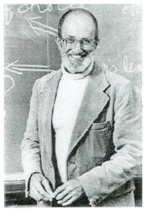
\includegraphics[scale=.8]{halmos}
\captionof{figure}{In \textit{How to Write Mathematics} P.R. Halmos writes: `This is a subjective essay, and its title is misleading; a more honest title might be `How I Write Mathematics'.}
\end{marginfigure}

\newthought{Choose your notation carefully}

Bad notation can make good exposition bad and bad exposition worse; ad hoc decisions about notation, made mid-sentence in the heat of composition, are almost certain to result in bad notation. Good notation has a kind of alphabetical harmony and avoids dissonance. Example: either + by$ or +a_2x_2$ is preferable to $bx_2$. Or: if you must use $\Sigma$ for an index set, make sure you don't run into $\sum_{\sigma \in \Sigma}a_\sigma$. Along the same lines: perhaps most readers wouldn't notice that you used $Izl$.

\newthought{One symbol, one letter}

A mathematical symbol is usually indicated by \emph{one} letter, not two or three. If for example we want to suggest that the \textit{factor of safety} is equal to three, we should write
\[F_{\mathrm{s}}=3\]
and not
\[F_{\mathrm{safetyfactor}}=3\]
or worse
\[F_{\mathrm{sf}}=3\]
typesetting the subscript in \textit{italic} font is also wrong
\[F_{s}=3\]
as it does not represent a mathematical symbol, but is just an abbreviation for safety factor.

Sometimes the use of the one symbol one letter rule cannot be applied, without the notation becoming complex
\medskip

{
\narrower\narrower
The static friction force \(F_{\mathrm{sf}}\) will exactly oppose forces applied to an object parallel to a surface contact up to the limit specified by the [[coefficient of static friction]] \(\mu_{\mathrm{sf}}\) multiplied by the normal force \(F_N\). In other words the magnitude of the static friction force satisfies the inequality:

\[ \le F_{\mathrm{sf}} \le \mu_{\mathrm{sf}} F_\mathrm{N}. \]

The kinetic friction force \(F_{\mathrm{kf}}\) is independent of both the forces applied and the movement of the object. Thus, the magnitude of the force equals:

\[F_{\mathrm{kf}} = \mu_{\mathrm{kf}} F_\mathrm{N}\]

where \(\mu_{\mathrm{kf}}\) is the coefficient of kinetic friction.
}




\newthought{Do not start a sentence with an equation}

\newthought{Display math}

In general mathematics typeset better when they are displayed. Use inline maths only for the simplest of equations and for explanations of symbols and the like. watch out for inconsistent spacing before and after displayed math.

\newthought{Correct badly sized math}

Some \tex constructions typeset rather badly, consider for example this:

\[
\sqrt{\frac{\beta}{\gamma}} = \sqrt{X} + \sqrt{y}
\]

\noindent or this,

\[
\surd{\frac{\beta}{\gamma}} = \surd{X} + \surd{y}
\]


You can remedy this by using a \cmd{mathstrut}.


\emphasis{sqrt,mathstrut}
\begin{teXX}
\sqrt{\mathstrut a}=\sqrt{\mathstrut X}+\sqrt{\mathstrut y}
\end{teXX}

\newthought{Multiplication}

One of the most common errors is to use the ``dot'' to indicate multiplication between scalars\sidenote{\url{http://www.tug.org/TUGboat/Articles/tb29-2/tb92guiggiani.pdf}}. For example the folowing formul\ae
\[a\cdot x^2+b\cdot x+c=0\]
should be written as
\[ax^2+bx+c=0\]

In fact, for the the sake of simplicity, the standard multiplication between letters, or between letters, or between a number and a letter, does not require any symbol. If, on the other hand, the multiplication is between two numbers, the $\times$ or $\cdot$ symbols are required to avoid ambiguity.
For example you should write

\[2\times 3=6 \text{ and not } 2\thickspace 3=6 \]


\newthought{Using the right font}

The Euler equation involves the five most important mathematical constants. First we typest it with no space corrections\sidenote{\texttt{\textbackslash eu\^\,\{\textbackslash iu\textbackslash pi\}}},
% The number `e'
\providecommand*{\eu}%
{\ensuremath{\mathrm{e}}}
% The imaginary unit
\providecommand*{\iu}%
{\ensuremath{\mathrm{j}}}
\[\scalebox{3}{$\eu^{\iu\pi}$}\]
a small correction to the space should be added

\[\scalebox{3}{$\eu^{\,\iu\pi}$}\]

\subsection{Differential operators}
A peculiar defnition is required to properly
write the differential symbol. It is in fact an operator that has a space only on its left. In Beccari (2007b) the following solution is proposed:

\bigskip


\clearpage
\section{tikz}
\begin{tcblisting}{colback=blue!5,boxrule=2pt,colframe=blue!75!black,title=Basic Definitions,width=0.75\textwidth}
because of the periodicity of the Jacobi theta functions involved in the construction of the vectors.
The height difference between starting point and endpoint of the path is thus $Lp$ as shown in figure \ref{fig:path}. Moreover, because of the periodicity of the theta functions it is sufficient to restrict the initial height to $\ell_1=0,1,\dots,L-1$ in this case.
  \centering
  \begin{tikzpicture}[>=stealth]
     \draw[scale=0.5,thick] (0,0)--(2,2)--(3,1)--(5,3)--(6,2)--(7,3);
           
     \draw[<->] (0,2) -- (0,-0.5) -- (4,-0.5);
     \foreach \x in {0.25,0.75,...,3.25}
       \draw[xshift=\x cm,yshift=-0.5cm] (0,-0.075)--(0,0.075);
     
    \foreach \y in {-0.5,0,...,1.5}
       \draw[yshift=\y cm] (-0.075,0)--(0.075,0);
 
    \draw (0.25,-0.5) node[below] {$1$};
    \draw (0.75,-0.5) node[below] {$2$};
    \draw (2,-0.5) node[below] {$\cdots$};
    \draw (3.25,-0.5) node[below] {$N$};
    \draw (4,-0.5) node[below] {$j$};
    \draw (0,0) node [left] {$\ell$};
    \draw (0,1.5) node [left] {$\ell+Lp$};
    \draw (0,2) node [right] {$\ell_j$};
     \clip[scale=0.5] (0,-1.5) rectangle (7.5,3.5);
     \draw[scale=0.5,dotted] (-1,-2) grid (8,5);
  \end{tikzpicture}
\end{tcblisting}
\clearpage


\begin{tcblisting}{colback=blue!5,boxrule=2pt,colframe=blue!75!black,title=Basic Definitions,width=0.75\textwidth}
\newcommand{\ud}{\ensuremath \mathop{}\!\mathrm{d}}
\(z=2\sin x\mathrm{d}x\) and \(z=2\sin x\ud x\)
\end{tcblisting}
\newcommand{\ud}{\mathop{}\!\mathrm{d}}
\bigskip

It uses an empty operator and eliminates the space
on its left with |\!|.

Note the difference between

\[z=2\sin x\mathrm{d}x  \]

\[z=2\sin x\ud x\]

where the diffrential is obtained respectively with
|\mathrm{d}| and |\ud|.

\newthought{God is in the details}

Sometimes you will be faced with small decisions for which the Journal style manual might not have an answer for you or the editor might have a different opinion to yours. One such question is if one needs to insert the thousand separator in coefficients.

\[
\operatorname{erf}^{-1}(z)=\tfrac{1}{2}\sqrt{\pi}\left (z+\frac{\pi}{12}z^3+\frac{7\pi^2}{480}z^5+\frac{127\pi^3}{40320}z^7+\frac{4369\pi^4}{5806080}z^9+\frac{34807\pi^5}{182476800}z^{11}+\cdots\right )
\]


\[
\operatorname{erf}^{-1}(z)=\tfrac{1}{2}\sqrt{\pi}\left (z+\frac{\pi}{12}z^3+\frac{7\pi^2}{480}z^5+\frac{127\pi^3}{40,320}z^7+\frac{4,369\pi^4}{5,806,080}z^9+\frac{34,807\pi^5}{182,476,800}z^{11}+\cdots\right )
\]

\[
\operatorname{erf}^{-1}(z)=\tfrac{1}{2}\sqrt{\pi}\left (z+\frac{\pi}{12}z^3+\frac{7\pi^2}{480}z^5+\frac{127\pi^3}{40{,}320}z^7+\frac{4{,}369\pi^4}{5{,}806{,}080}z^9+\frac{34{,}807\pi^5}{182{,}476,800}z^{11}+\cdots\right )
\]



\[
\operatorname{erf}^{-1}(z)=\tfrac{1}{2}\sqrt{\pi}\left (z+\frac{\pi}{12}z^3+\frac{7\pi^2}{480}z^5+\frac{127\pi^3}{40\thinspace 320}z^7+\frac{4\thinspace 369\pi^4}{5\thinspace 806\thinspace 080}z^9+\frac{34\thinspace 807\pi^5}{182\thinspace 476\thinspace 800}z^{11}+\cdots\right )
\]


It is interesting to note that Knuth believes that in equations this is unecessary.
He is quoted in Typesetting Mathematics.

\begin{quotation}
But where Don wrote 1000000 they substituted
1,000,000. Don objected that although this might be justifed in text, his use is perfectly OK in a formula. Well then, they replied, write \(10^6\).
Fine, said, Don, but what do I do 
when the number is 1234567? The IEEE standard here is to insert spaces, thus: 1 234 567.
Don doesn't like this in formulae, but agrees that it may be useful in a high precision context, such as numerical tables. 
\end{quotation}

The following are extracts from his paper \sidenote{\url{http://www-cs-faculty.stanford.edu/~uno/papers/jfsp.tex.gz}}

{
$$\vcenter{\halign{$#$\hfil\ &$#$\hfil\cr
\Sigma n^{11}&=39916800{n+6\choose 12}+
19958400{n+5\choose 10}+3160080{n+4\choose 8}
+168960{n+3\choose 6}\cr
\noalign{\smallskip}
&\qquad\null+2046{n+2\choose 4}+{n+1\choose 2}\,;\cr
\noalign{\smallskip}
\Sigma n^{13}&=6227020800{n+7\choose 14}+3632428800{n+6\choose 12}+
726485760{n+5\choose 10}\cr
\noalign{\smallskip}
&\qquad\null+57657600{n+4\choose 8}
+1561560{n+3\choose 6}+8190{n+2\choose 4}+{n+1\choose 2}\,.\cr}}$$
}

Also, note in the last equation the use of a period at the end. This is something that strong opinions and flaming wars in fora. I am not too sure if I agree on the last one, but the way that Knuth writes is very clear and his equations in a way are paragraphs. In this case the use of a period is recommended.


\newthought{Punctuation}

There are two schools of thought when it comes to punctuation, that is punctuation in display style formulae. Some authors (Beccari,2007 a), others that it is necessary and essential.

The authors of this article believe that formulae,
both in display and text style, are part of the argumentation
and so punctuation should be used to help
the reader. An example of good use of punctuation is:


Since
$$ a=b $$
and
$$b=c,$$
it is proven that
\[a =c. \]



\subsection{Numbering Equations}

One question that you may face is the numbering of display equations. Early books used numbering sparingly, whereas many authors go overboard and number all the equations.

According to Knuth et al:\footnote{\url{http://tex.loria.fr/typographie/mathwriting.pdf}}

Numbering all displayed formulas is usually a bad idea; number the important ones only.
Halmos\footnote{\url{http://www.math.uh.edu/~tomforde/Books/Halmos-How-To-Write.pdf}} offers pretty much the same good advice,

\begin{quotation}
What about "inequality (*)", or "equation (7)", or "formula (iii)"; should all displays be labelled or numbered? My answer is no. Reason: just as you shouldn't mention irrelevant assumptions or name irrelevant concepts, you also shouldn't attach irrelevant labels. Some small part of the reader's attention is attracted to the label, and some small part of his mind will wonder why the label is there. If there is a reason, then the wonder serves a healthy purpose by way of preparation, with no fuss, for a future reference to the same idea; if there is no reason, then the attention and the wonder were wasted.
\end{quotation}

See also discussion at \url{http://tex.stackexchange.com/questions/29267/which-equations-should-be numbered/49080\#49080}

\url{http://tex.stackexchange.com/questions/29267/which-equations-should-be-numbered/49080#49080}

Now if you wish to argue about this is fine.

\section{Mathmode}

TeX is in mathmode when it is reading mathematics. The |ifmmode| can be used to find out if TeX is in math mode. It denotes the start of an if-then-else control structure that tests whether \tex is currently in either math mode or display math mode. The |\else| part is optional. <TeX code 1> is processed if TeX is in one of the math modes, otherwise it is ignored. If the |\else| section is included and TeX is not in one of the math modes then <TeX code 2> is processed; otherwise it is ignored.

%\begin{teXXX}
%\def\A{\ifmmode \mathcal{A} \else $\mathcal{A}$ \fi}
%\end{teXXX}

\begin{tcblisting}{}
 \def\a{test}
\a
\end{tcblisting}
\medskip
\begin{tcolorbox}[colback=blue!5,boxrule=2pt,boxsep=3mm,colframe=blue!75!black,title=Basic Definitions,width=0.65\textwidth]
    |\def\A{\ifmmode \mathcal{A} \else \[\mathcal{A}\] \fi}|
\end{tcolorbox}
\medskip


defines a macro |\A| that can be used both in and out of math mode to typeset a calligraphy script A. 

This is a calligraphic \A\ or $\A$.


\[ \A \]


\clearpage
\section{Useful packages}
Besides the main packages that we have discussed so far and which should be in everyone's toolbox, there are a number of other packages that you may find useful. One such package is the |\multienum|, which although not really a packaged specializing in mathematical typesetting, it provides an environment to set multiple equations, as in an exercise or exam.

%\begin{teXXX}
%\documentclass{article}
%\usepackage{xstring,amsmath}
%\begin{document}
%\[\operatornamewithlimits{K}_{k=0}^\infty\frac{a_k}{b_k}\]
%\end{document}
%
%\end{teXXX}


\newthought{the multienum package}

The \docpkg{multienum} enables  the typestting of multiple equations on one line and numbering them, either with roman, arabic or alpha letters.

\emphasis{usepackage, multienum,begin,end,multienumerate}
\begin{teXXX}
\documentclass{article}
\usepackage{multienum}
\renewcommand{\regularlisti}{\setcounter{multienumi}{0}%
  \renewcommand{\labelenumi}%
  {\addtocounter{multienumi}{1}\alph{multienumi})}}
\begin{document}
\begin{multienumerate}[oddlist]
\mitemxxx{\(x^2 + y^2 = 1\)}{\(a + b = c\)}{\(r-x = y+z\)}
\mitemxxx{\(f - y = z\)}{\(a - b = 2d\)}{\(r+x = 2y-3z\)}
\end{multienumerate}
\end{document}
\end{teXXX}


\begin{multienumerate}[oddlist]
\mitemxxx{\(x^2 + y^2 = 1\)}{\(a + b = c\)}{\(r-x = y+z\)}
\end{multienumerate}
\begin{multienumerate}[evenlist]
\mitemxxx{\(f - y = z\)}{\(a - b = 2d\)}{\(r+x = 2y-3z\)}
\end{multienumerate}


\hrule

\bigskip

We can also enumerate the items using an even-only or odd only
counter.
\subsection*{Answers to Even-Numbered Exercises}
\begin{multienumerate}[evenlist]
\mitemxxxx{Not}{Linear}{Not}{Quadratic}
\mitemxxxo{Not}{Linear}{No; if $x=3$, then $y=-2$.}
\mitemxx{$(x_1,x_2)=(2+\frac{1}{3}t,t)$ or
$(s,3s-6)$}{$(x_1,x_2,x_3)=(2+\frac{5}{2}s-3t,s,t)$}
\mitemx{$(x_1,x_2,x_3,x_4)= (\frac{1}{4}+\frac{5}{4}s+\frac{3}{4}t-u,s,t,u)$
or $(s,t,u,\frac{1}{4}-s+\frac{5}{4}t+\frac{3}{4}u)$}
\mitemxxxx{$(2,-1,3)$}{None}{$(2,1,0,1)$}{$(0,0,0,0)$}
\end{multienumerate}
\bigskip

\hrule

\clearpage


\begin{casestudy}[The Riemann hypothesis.]{%
Typeset the text and the equations, shown below. Use a standard minimal to achieve it. Note the fraktur fonts. Text must all be as one paragraph.}

It is well known that the Riemann zeta function $\zeta(s)$ of a complex variable $s=\sigma+it$ is defined by
\[
\zeta(s)=\sum_{n=1}^{\infty}\frac{1}{n^{s}}
\]
for the real part $\mathfrak{R}(s)>1$ and its analytic continuation in the half plane $\sigma>0$ is
\begin{equation}\label{func:zeta}
\zeta(s)=\sum_{n=1}^{N}\frac{1}{n^{s}}-\frac{N^{1-s}}{1-s}-\frac{1}{2}N^{-s}
+s\int_{N}^{\infty}\frac{\frac{1}{2}-\{x\}}{x^{s+1}}dx
\end{equation}
for any integer $N\geq1$ and $\mathfrak{R}(s)>0$.
It extends to an analytic function in the whole complex plane except for having a simple pole at $s=1$. Trivially, $\zeta(-2n)=0$ for all positive integers. All other zeros of the Riemann zeta functions are called its nontrivial zeros.
\bottomline

\begin{teX}
It is well known that the Riemann zeta function $\zeta(s)$ of a complex variable $s=\sigma+it$ is defined by
\[
\zeta(s)=\sum_{n=1}^{\infty}\frac{1}{n^{s}}
\]
for the real part $\mathfrak{R}(s)>1$ and its analytic continuation in the half plane $\sigma>0$ is
\begin{equation}\label{func:zeta}
\zeta(s)=\sum_{n=1}^{N}\frac{1}{n^{s}}-\frac{N^{1-s}}{1-s}-\frac{1}{2}N^{-s}
+s\int_{N}^{\infty}\frac{\frac{1}{2}-\{x\}}{x^{s+1}}dx
\end{equation}
for any integer $N\geq1$ and $\mathfrak{R}(s)>0$.
It extends to an analytic function in the whole complex plane except for having a simple pole at $s=1$. Trivially, $\zeta(-2n)=0$ for all positive integers. All other zeros of the Riemann zeta functions are called its nontrivial zeros.
\end{teX}

Please note that the maths and the text, are typed as a single block. Do not leave any spaces in between. We have used |\mathfrak| for the fraktur font. We have also used $it$ for the imaginary part. This would depend on the style used in your field. 
\end{casestudy}

\clearpage
\section{Gather}
This is like a multi line environment with no special horizontal alignment. All rows
are centered and can have an own equation number:

\begin{tcblisting}{colback=blue!5,boxrule=2pt,colframe=blue!75!black,title=The gather environment,width=\textwidth,before=\bigskip,after=\bigskip}
\def\O{\mathcal{O}}
\begin{gather}
 \O,\O(E_4),\O(E_2),\O(H-E_3-E_5),\O(H-E_3),\O(H-E_5),\\ 
\O(2H-E_1-E_3-E_5-E_6),\O(2H-E_1-E_3-E_5),\O(2H-E_3-E_5-E_6).
\end{gather}

So lautet der Beweis des Satzes $2 \times 2 = 4$:
\begin{gather}
(\Omega^{\nu})^{\mu}{}'x = \Omega^{\nu \times \mu}{}'x \text{ Def.}\\
%\begin{split}
\Omega^{2 \times 2}{}'x = (\Omega^{2})^{2}{}'x = (\Omega^{2})^{1 + 1}{}'x = \Omega^{2}{}'\Omega^{2}{}'x = \Omega^{1 + 1}{}'\Omega^{1 + 1}{}'x\nonumber \\
= (\Omega'\Omega)'(\Omega'\Omega)'x = \Omega'\Omega'\Omega'\Omega'x = \Omega^{1 + 1 + 1 + 1}{}'x = \Omega^{4}{}'x.
%\end{split}
\end{gather}


\begin{gather*}
x = \Omega^{0}{}' x \text{ Def.\ and}\\
\Omega'\Omega^{\nu}{}'x = \Omega^{\nu+1}{}'x \text{ Def.}
\end{gather*}
\begin{equation}
x = \Omega^{0}{}' x \text{ Def.\ and}\\
\Omega'\Omega^{\nu}{}'x = \Omega^{\nu+1}{}'x \text{ Def.}
\end{equation}
\end{tcblisting}


The gather environment has an implicit |{c}| horizontal alignment with no
vertical column alignment. It is just like an one column array/table.
A nonumber-version |\begin{gather*}...\end{gather*}| exists. 

A common error is to forget the include `\$\$` in intertext text, if you want to include
maths as part of the textual description.

\emphasis{intertext}
\begin{tcblisting}{colback=blue!5,boxrule=2pt,colframe=blue!75!black,title=The gather environment,width=\textwidth,before=\bigskip,after=\bigskip}
\def\mat#1{\bm{\mathrm{#1}}}
\begin{align}
	 A &= \frac{1}{\sqrt{2}}
	\begin{pmatrix}
		1	&	1	\\
		i e^{-2 r_2}	&	-i e^{-2 r_2}
	\end{pmatrix}
	\,, \\
	B &= \frac{1}{\sqrt{2}}
	\begin{pmatrix}
		i e^{-2 r_1}	&	i e^{-2 r_1}	\\
		-1	&	1
	\end{pmatrix}
	\,,\\
\intertext{note that $z = i e^{r_1}$}
	A^{-1} &= \frac{1}{\sqrt{2}}
	\begin{pmatrix}
		1	&	-i e^{+2 r_2}	\\
		1	&	i e^{+2 r_2}
	\end{pmatrix}
	\,,
\end{align}
\end{tcblisting}




left to curl \left\{\begin{matrix}
first \\
second \\ 
42
\end{matrix}\right.

\end{document}

\chapter{Drawing pictures and graphs}
\epigraph{Dear God\break If I have but one hour remaining to live, please allow me to spend this time
in a mathematics class so that it will seem to last forever.}{\textit{---A bored student's prayer}}


\begin{figure}%
  \centering
  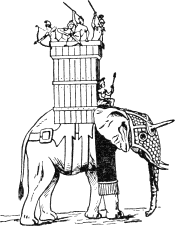
\includegraphics[width=0.3\linewidth]{./graphics/pic37.png}
  \caption{During the early days of typography fonts were designed to emulate the looks of calligraphic texts.}
  \label{fig:marginfig1}
\end{figure}

\section{Inserting figures}

In order to insert figures, the \pkgname{graphicx} package has to included in the preamble (before the |\begin{document}|-command) of your LaTeX-document:

\graybox{\texttt{\textbackslash usepackage\{graphicx\}}}

Originally only EPS-figures could be inserted with the \pkgname{graphic}package. This has now been developed into the  \pkgname{graphicx}, which allows almost any common format to be inserted. 

The simplest way of including a graphic looks like this:


\CMDI{\includegraphics}\marg{filename}


If the image is not located in the same folder as the tex-file, you will have to specify the path relative to the tex-file.

\graybox{\texttt{\textbackslash includegraphics\{./images/filename\}}}


\subsection{Scaling and resizing images}

If you want the image to appear in a different size, you can specifiy the size as a parameter of the |\includegraphics|-command::


\graybox{\texttt{\textbackslash includegraphics[width=3.9cm]\{filename\}}}


This will scale the image to the width of 3.9 centimeters. 

Use |\textwidth| command if you don't want to specify an absolute size but rather want the actual size to depend on the text width of the page. You can use any of the normal \tex units such as \texttt{em, pt, cm, in}:
\graybox{\texttt{\textbackslash includegraphics[width=0.5\textbackslash textwidth]\{filename\}}}
\noindent will scale the image to half of the text width. The images in the
figure below were produced by two |includegraphics| commands. You can have as many as you like and the \tex engine will treat them the same way as text. If you a leave a space between the commands, they will be positioned vertically as they are treated as paragraphs.

\medskip
\begingroup

\centering
\includegraphics[width=0.3\textwidth]{./graphics/amato.jpg}
\includegraphics[width=0.3\textwidth]{./graphics/amato.jpg}
\includegraphics[width=0.3\textwidth]{./graphics/amato.jpg}

\endgroup


The three photos were centered using the |\centering| command, within a group.


\begin{teX}
\begingroup

\centering
\includegraphics[width=0.3\textwidth]{./graphics/amato.jpg}
\includegraphics[width=0.3\textwidth]{./graphics/amato.jpg}
\includegraphics[width=0.3\textwidth]{./graphics/amato.jpg}
\endgroup
\end{teX}

The |\begingroup..\endgroup| is necessary to limit the effect of centering to
the group only, otherwise \tex would center everything from this point onwards.

\subsection{Controlling the aspect ratio}

You can control the picture aspect ratio by using the command:

\CMDI{\includegraphics}[keepaspectratio,width=3cm, height=3cm]]\{filename\}


If set to true then specifying 
both |width| and |height| (or |totalheight|) does not distort the figure but 
scales such that neither of the specified dimensions is exceeded.






\medskip
\begingroup

\centering
\includegraphics[width=0.3\textwidth, height=5cm]{./images/amato.jpg}
\includegraphics[keepaspectratio=true,width=4cm, height=5cm]{./images/amato.jpg}
\includegraphics[width=3cm]{./images/amato.jpg}

\endgroup


This can be very useful if you have images shown side by side with different
aspect ratios. 


\subsection{Paths and file types}

For larger projects you will probably find it more convenient to have 
images in different folders. You can specify default paths using:


\CMDI{\graphicspath}\marg{dir-list}

This optional declaration may be used to specify a list of directories in which to
search for graphics files. The format is the same as for the \latexe primitive
|\input@path|. A list of directories, each in a \{\} group (even if there is only one
in the list). For example:


\graybox{\texttt{\textbackslash graphicspath\{\{eps/\}\{tiff/\}\}}}


The default image formats can be declared using:

\CMDI{\DeclareGraphicsExtensions}\marg{png,jpg}

This specifies the behaviour of the system when no file extension is specified in 
the argument to |\includegraphics|. \texttt{\{ext-list\}} should be a comma separated 
list of file extensions. (White space is ignored between the entries.) A file name
is produced by appending one extension from the list. If a file is found, the
system acts as if that extension had been specified. If not, the next extension
in \texttt{ext-list} is tried.



\subsection{The figure environment}

You use the figure-environment to let your image appear in a "floating" environment, that is \latex will place it at the right position of a page and even on the next page:

\begin{teX}
\begin{figure}
  \includegraphics{filename.eps}
  \caption{title of your figure}
  \label{labelname}
\end{figure}
\end{teX}

Here |\caption{...}| defines the title of the figure which will appear beneath the figure. |\label{..}| defines the label which can be used inside the document in order to insert references to the figure:

The figure

|\ref{labelname} on page \pageref{labelname} ..|

The|\label-command| inside the |\figure|-envirnonment hast to appear just after the|\caption|-command.
placing figures

If figures reside inside a |\figure|-environment, this will cause LaTeX to choose the actual location of the figure inside the document. There are different parameters for the placement strategy:

\begin{description}
\item[h (here)] Try to place the figure just where the command is located.

\item [t (top)] Try to place the figure at the top of the page.

\item[b (bottom)] Try to place the figure at the bottom of the page.

\item [p (float page)] Try to place the figure on a page which contains only floating elements.
\end{description}

The order of these parameters doesn't matter since placement is always tried in the order \textbf{h, t, b, p,} if these parameters are present:

If no parameter is present, the default order is  \texttt{[tbp]}.


The command for a figure-environment might for example look like this:

\begin{teX}
\begin{figure}[htbp]
...
\end{figure}
\end{teX}



\subsection{Table of figures}
\index{figures!Table of figures}
A table of figures is inserted (where you place the command) using the command


\begin{teX}
   \listoffigures
\end{teX}

The caption given in the \cmd{caption} command is also used in the list of figures. 
If you want to use different captions, you may add a parameter to the |\caption| command:
|\caption[caption for listoffigures]{caption inside the document}|


\subsection{Figures with a border}

Although drawing frames around tables should be discouraged, if you find the need
to draw them there are  two possible ways to achieve it: either only the figure itself is bordered or there is a border around the figure and its caption. You place a border around the figure using the \cmd{\fbox} command or the \cmd{\framebox}.

\emphasis{fbox,minipage}
\begin{teX}
\begin{figure}[htbp]
  \centering
  \fbox{
    \includegraphics{filename}
  }
  \caption{caption}
  \label{Labelname}
\end{figure}
\end{teX}

Placing a border around the figure and its title is a little more tricky: You need to place the figure and the title in a |\minipage| environment which is bordered again with the |\fbox| command:

\begin{teX}
\begin{figure}[htbp]
  \centering
  \fbox{
    \begin{minipage}{13 cm}
      \includegraphics{filename}
      \caption{caption}
      \label{labelname}
    \end{minipage}
  }
\end{figure}
\end{teX}

This will produce the image shown below,

\begin{center}
\begin{figure}[htbp]
  \centering
  \fbox{
    \begin{minipage}{0.25\linewidth}
      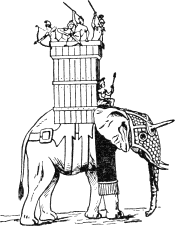
\includegraphics[width=0.9\linewidth]{./graphics/pic37.png}
      \caption{The boxed fighting elephant}
      \label{labelname}
    \end{minipage}
  }
\end{figure}
\end{center}


Unfortunately the width of the border cannot be determined automatically. It has to be specified as a parameter of the |\minipage| environment. However, you may be bale to develop a macro to do this - based on the ImageSize routines we developed in section.


\section{Side by side figures}

You might want to place to figures side by side but to use only one caption. This is achieved by placing both figures in its own |\minipage| which reside in the same |\figure|.

if only one |\caption| command is used, both figures will have a common title:

\medskip
\begin{verbatim}
\begin{figure}[htbp]
  \centering
  \begin{minipage}[b]{5 cm}
    \includegraphics{filename 1}  
  \end{minipage}
  \begin{minipage}[b]{5 cm}
    \includegraphics{filename 2}  
  \end{minipage}
  \caption{common caption}
  \label{Labelname}
\end{figure}
\end{verbatim}
\medskip

The first parameter of the |\minipage| environment determines how both graphics are aligned to each other. b (bottom) aligns the bottom borders of the figures, \textbf{t} (top) aligns the top borders and \textbf{c} aligns the centers.

If you want distinct titles for the two figures you will only have to supply a |\caption| command for both |\minipage|environments:

\begin{teX}
\begin{figure}[htbp]
  \centering
  \begin{minipage}[b]{5 cm}
    \includegraphics{filename 1} 
    \caption{caption 1}
    \label{labelname 1}
  \end{minipage}
  \begin{minipage}[b]{5 cm}
    \includegraphics{filename 2}  
    \caption{caption 2}
    \label{labelname 2}
  \end{minipage}
\end{figure}
\end{teX}


If you want to have subfigures with distinct caption, you use the |\subfig| package:


You can put as many figures as you like on a page, but a word of warning, you may need to make some manual adjustments before you get it right. The package provides support for the manipulation and reference of small or ‘sub’ floats within a single floating (e.g., figure or table) environment1 It is convenient to use this
package when your sub-floats are to be separately captioned, referenced, or when such
sub-captions are to be included on a List-of-Floats page.

The package is a replacement for the subfigure package, from which it was derived.
However, the new subfig package is not completely backward compatible.
Therefore, a new name was called for. The newer package is smaller and easier to use
than the older package, however, it now uses the following additional packages, 
caption (required), 
everysel (optional), 
keyval (required), 
ragged2e (optional).

It will work without the ragged2e and everysel packages if you do not use the following
justification options: ‘Center’, ‘RaggedRight’ and ‘RaggedLeft’. The other justification
options ‘center’, ‘raggedright’ and ‘raggedleft’ will work without the above two packages. If the ragged2e package is present, than the caption package will load it and it
will, in turn, load the everysel package. This happens whether or not you will be using
the justification options that require it. If it cannot find the ragged2e package, than the
caption package will print a message that ‘RaggedRight’, etc. will not be available.



 A low bottle-shaped vase, of yellowish ware, with flaring rim and somewhat flattened body. Height, 5 inches; width 5 inches. \ref{fig:one}

A well-made bottle shaped vase, with low neck and globular body, somewhat conical above. Color dark brownish. 7½ inches in height. Shown in \ref{fig:two}


\begin{figure}
  \centering
  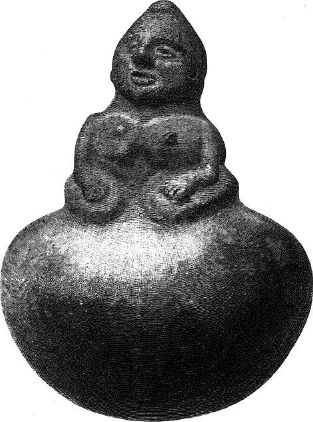
\includegraphics[width=0.7\linewidth]{./graphics/fig175.jpg}
   \centerline{From the tomb of a Pull\= arius.}
  \label{fig:marginfig1}
\end{figure}

The above figure is an effigy vase of the dark ware. The body is globular. A kneeling human figure forms the neck. The mouth of the vessel occurs at the back of the head—a rule in this class of vessels. Is is finely made and symmetrical. 9¾ inches high and 7 inches in diameter. being larger than the above two it is preferable to scale it to give the reader an indication. Based on the figure width, you may also need to adjust the distance between the figures to ensure that the whitespace is just about right. For screen reading this can be increased and for printed works you may wish to make it less.







\section{The wrapfig package}


\captionsetup[wrapfigure]{margin=10pt,font=small,labelfont=bf, name=Fig.} % [wrapfigure]{name=Fig.}


Donald Arseneau has created the \pkg{wrapfig} package to allow people to place figures or
tables at the side of a page and wrap text around them. The package provides the
environments wrapfigure and wraptable. Both environments have two required and
two optional arguments. You can see an example taht uses the package to wrap a picture into such a paragraph of text.

\begin{figure}[82pt]
   \includegraphics[width=\linewidth]{./graphics/cyprus.jpg} 
   \caption{\small Cyprian limestone group of Phoenician dancers, about 6½ in. high. There is a somewhat similar group, also from Cyprus, in the British Museum. The dress, a hooded cowl, appears to be of great antiquity.}
\end{figure}

\begin{wrapfigure}[20]{l}{3.8cm}
\centering\small
\includegraphics[width=\linewidth]{./graphics/egyptdance.jpg}  
\caption{\small The hieroglyphics describe the dance.}
\end{wrapfigure}
Amongst the earliest representations that are comprehensible, we have certain Egyptian paintings, and some of these exhibit postures that evidently had even then a settled meaning, and were a phrase in the sentences of the art. Not only were they settled at such an early period (B.C. 3000, fig. 1) but they appear to have been accepted and handed down to succeeding generations (fig. 2), and what is remarkable in some countries, even to our own times. The accompanying illustrations from Egypt and Greece exhibit what was evidently a traditional attitude. The hand-in-hand dance is another of these.

The earliest accompaniments to dancing appear to have been the clapping of hands, the pipes,[1] the guitar, the tambourine, the castanets, the cymbals, the tambour, and sometimes in the street, the drum.

The following account of Egyptian dancing is from Sir Gardiner Wilkinson's "Ancient Egypt"[2]:—
\begin{figure}
   \includegraphics[width=0.3\linewidth]{./graphics/lotus.jpg} 
   \caption{\small Cyprian limestone group of Phoenician dancers, about 6½ in. high. There is a somewhat similar group, also from Cyprus, in the British Museum. The dress, a hooded cowl, appears to be of great antiquity.}
\end{figure}
"The dance consisted mostly of a succession of figures, in which the performers endeavoured to exhibit a great variety of gesture. Men and women danced at the same time, or in separate parties, but the latter were generally preferred for their superior grace and elegance. Some danced to slow airs, adapted to the style of their movement; the attitudes they assumed frequently partook of a grace not unworthy of the Greeks; and some credit is due to the skill of the artist who represented the subject, which excites additional interest from its being in one of the oldest tombs of Thebes (B.C. 1450, Amenophis II.). Others preferred a lively step, regulated by an appropriate tune; and men sometimes danced with great spirit, bounding from the ground, more in the manner of Europeans than of Eastern people. On these occasions the music was not always composed of many instruments, and here we find only the cylindrical maces and a woman snapping her fingers in the time, in lieu of cymbals or castanets.

\begin{figure}
   \includegraphics[width=0.3\linewidth]{./graphics/patera.jpg} 
   \caption{\small Cyprian limestone group of Phoenician dancers, about 6½ in. high. There is a somewhat similar group, also from Cyprus, in the British Museum. The dress, a hooded cowl, appears to be of great antiquity.}
\end{figure}

"Graceful attitudes and gesticulations were the general style of their dance, but, as in all other countries, the taste of the performance varied according to the rank of the person by whom they were employed, or their own skill, and the dance at the house of a priest differed from that among the uncouth peasantry, etc.

"It was not customary for the upper orders of Egyptians to indulge in this amusement, either in public or private assemblies, and none appear to have practised it but the lower ranks of society, and those who gained their livelihood by attending festive meetings.

"Many of these postures resembled those of the modern ballet, and the pirouette delighted an Egyptian party 3,500 years ago.
\medskip

The wrapped figure is positioned using the \texttt{wrapfigure} environment, as shown below:

\begin{teX}
\begin{wrapfigure}[nlines]{placement}[overhang ]{width }
   \includegraphics[width=3.8cm]{./graphics/egyptdance} 
   \caption{\small The hieroglyphics describe the dance.}
\end{wrapfigure}
\end{teX}

The parameter |nlines|  is the number of narrow lines, and placement is one of r, l, i, o, R, L, I, or
O for right, le, inside, and outside, respectively. The uppercase placement specifiers
differ from their lowercase counterparts in that they force \latex to put the float \emph{here},
whereas the lowercase placement specifiers just give a hint to \latex to place them
\texttt{here}. The \texttt{width} argument is the width of the figure or table that appears in the body
of the environment. Finally, \texttt{overhang} tells LATEX how much the figure should hang out
into the margin of the page. Here is how one may create dangerous paragraphs bends!

The |wrapfig| package is compatible with the |caption| package. You can set the caption parameters using:---

\begin{teX}
\captionsetup[wrapfigure]{<options>}
\end{teX}

If you are probably wondering how |wrapfig| achieves this, you should read the class file. It basically uses |everypar|, and hence the limitations with |\par|. Here is an extract from the class.

\begin{teX}

% Subvert \everypar to float fig and do wrapping.  
% Also for non-float.
\def\WF@startfloating{%
 \WF@everypar\expandafter{\the\everypar}\let\everypar\WF@everypar
 \WF@@everypar{\ifvoid\WF@box\else\WF@floathand\fi \the\everypar
 \WF@wraphand
}}
\end{teX}

Moving now to a more scientific example that the previous ones, we will place two figures
one on top of each other and give them individual, sub-captions as shown in \ref{fig:honey}.
 
\captionsetup[figure]{margin=10pt,font=small,labelfont=bf,format=hang}%

\begin{figure}[htbp]
\centering
  \begin{subfigure}[b]{0.5\textwidth}
  \includegraphics[width=\linewidth]{./graphics/honey.png}
  \caption{Taylor instability in the surface of the honey in an inverted honey jar.}\label{fig:honey}
    \hspace{1cm}
  \end{subfigure}

  \begin{subfigure}[b]{0.9\textwidth}
     \centering
     \includegraphics[width=9cm]{./graphics/honeydrops.png}
     \caption{Taylor instability in the interface of the water condensing on the underside of a small water pipe.}
  \end{subfigure}  
  \caption{Two examples of Taylor instabilities that are commonly found.}%
    \label{fig:Athird}%
\end{figure}

The figures are from A Heat Transfer Textbook, by J.H.Lienhard, which incidentally was typeset using
\tex . It is a McGrawHill publication. 

\begin{teX}
\begin{figure}[htbp]
    \captionsetup[figure]{margin=10pt}%
    \subfloat[Taylor instability...]
     {{\includegraphics[width=8cm]{./graphics/honey}}}
    \hspace{1cm}
     \subfloat[Taylor instability in the...]%
      {\includegraphics[width=9cm]{./graphics/honeydrops}}  
     \\[-10pt]
   \caption{Taylor instability in...}%
    \label{fig:Afirst}%
    \caption{Two examples of... }%
    \label{fig:honey}%
\end{figure}
\end{teX}


The text can have more than one paragraph. It is also possible to include figures
generated by |TikZ/pgf|, as shown in the next example, drawn from real code
in the book.


\begin{wrapfigure}[14]{l}{3.0cm}
\pgfplotsset{width=5.0cm,compat=1.3}
\begin{tikzpicture}
\begin{axis}[minor y tick num=4, 
minor x tick num=4, 
xmin=0,xmax=300,
ymin=0,ymax=60,
xlabel=\textsf{liquidus ($l/s$)},
ylabel=\textsf{capitis ($m$)}, 
ytick={0,15,30,45,60,75},
xtick={0,100,200,300}
]
\addplot[color=blue,mark=x, smooth] coordinates {
(0,44)
(50,43)
(100,42)
(150,40)
(200,33)
(220,29)
};

\end{axis}
\end{tikzpicture}
\caption{Pump headum and flowm}
\end{wrapfigure}


\providecommand\addcredit[1]{%
 \vspace*{-6.5pt}
 \scriptsize%
 \flushright%
 \textit{Credit: #1}%
}
\newpage
\pagestyle{empty}
\thispagestyle{empty}
\begin{figure}[htp]
\centering

\captionsetup{name=Photo., labelsep=period}%
   \begin{minipage}[t]{0.48\textwidth}
      \includegraphics[width=\textwidth]{./graphics/movingup.jpg}%
      \addcredit{U.S. DoD.}%
     \caption{The effects of the credit going past the edge of the figure. This can be corrected by adding a minipage to hold both commands. }
\end{minipage}\hfill\hfill
\begin{minipage}[t]{0.48\textwidth}
      \includegraphics[width=\textwidth]{./graphics/survivors.jpg}%
      \addcredit{U.S. DoD.}%
    {\footnotesize Marines awaiting resting before moving on to Japan. }
\end{minipage}

% \begin{minipage}[t]{0.48\textwidth}
%      \includegraphics[width=\textwidth]{./graphics/img009.jpg}%
%      \addcredit{U.S. DoD.}%
%     \caption{Engineer Construction Troops in Liberia, July 1942.}
%\end{minipage}\hfill\hfill
%\begin{minipage}[t]{0.48\textwidth}
%      \includegraphics[width=\textwidth]{./graphics/survivors.jpg}%
%      \addcredit{U.S. DoD.}%
%     \caption{The effects of the credit going past the edge of the figure. This can be corrected by adding a minipage to hold both commands. }
%\end{minipage}
% \begin{minipage}[t]{0.48\textwidth}
%      \includegraphics[width=\textwidth]{./graphics/img126.jpg}%
%      \addcredit{U.S. DoD.}%
%     \caption{Marine Reinforcements.
%A light machine gun squad of 3d Battalion, 1st Marines, arrives during the battle for ``Boulder City.'' }
%\end{minipage}\hfill\hfill
%\begin{minipage}[t]{0.48\textwidth}
%      \includegraphics[width=\textwidth]{./graphics/img124.jpg}%
%      \addcredit{U.S. DoD.}%
%     \caption{Brothers Under the Skin, inductees at Fort Sam Houston, Texas, 1953. }
%\end{minipage}
\end{figure}
\newpage


Armed with all these packages you can help the Gutenburg organization to transcribe
some of the old books that they have online. 

\clearpage








\makeatletter\@specialfalse\@debugfalse\makeatother
\cxset{style13}
\cxset{title margin bottom=10pt}
\chapter{Introduction}
\addtocimage{-12pt}{-20pt}{../images/tocblock-fish.jpg}


\epigraph{``Begin at the beginning,'' the king said
"and then go on till you come to the end, then stop."}{
---Lewis Carroll, Alice in Wonderland}

\large

\noindent This package and its documentation attempts to eliminate some common 
problems encountered when using \LaTeX2e. The first one is the loading of 
recommended packages for a large and perhaps complicated document and 
the second is the re-designing of styles for a document.

 \LaTeX2e, does not provide a standard library, but comes equipped with
 a package mechanism that allows code extensions to be loaded as required.
 This has created a strong vibrant community, hundreds of packages and a 
 headache to both new and seasoned users. What packages are available, when
 to use them and in which order is a common theme for many questions on
 lists and |TX.SE|.

 It is quite common during the writing of a thesis or book
 for the author to keep on adding macros and packages
 at the preamble of the document. In most cases this can
 be satisfactory but in many others it leads to
 incompatibilities and errors. This package aims at
 minimizing one's preamble, by prefetching a number of
 commonly used packages. It also aims at loading them
 in the right order and providing patches for conflicts.
 
 I am hoping that using this package, will lead to less
 frustrations with the intricacies of \LaTeX2e\ packages.

The package code is complicated, but its usage is simple. You first load the package and then
you use one of the available templates:

 \begin{commands}[]{}
 \begin{verbatim}
 \usepackage{phd}
 \usetemplate{style13}
 \end{verbatim}
 \end{commands}

This is what you need to typeset a good looking book or thesis. The rest of this book is a footnote and you can skip them if you want. 

It will be better for the longer projects to just fork the
 package and adapt it to your needs. In this respect, I have
 uploaded the package to |github|.\footnote{\url{https://github.com/yannisl/phd}}

 My goal in selecting the packages and adding a number of 
 commands for the authors was to be able to typeset a 
 document for most common use cases, without the need of
 additional packages. The packages I selected are biased
 towards academic publications, although they can find use
 in almost any fields. The package provides a mechanism via
 PGF keys to provide a settings file. 
 
 Most of the documentation can be found in the implementation part.

Browse any books in a library or bookshop and the striking thing is that their design is very individualistic. They might have similarities but their main features vary. In many respects they resemble people's faces where minor differences have striking effects.

This package arose out of a question at stackexchange. How to redefine chapter heads. Having seen the popularity of the |pgf| package \cite{pkg-pgf} I realized that \latex users prefer this method of styling rather the traditional \latex method.

The user interface can be extended to basically all major packages. The principle is to keep to a minimum changes that can affect the LaTeX core commands. If there are any additions a key setting is provided to be able to revert back to normal LaTeX.

The workflow can be simplified. In addition I want to believe that the interface can provide a useful addition to the open source community and that other people will contribute style libraries, which will be simpler to write. It is also possible
to device an easy and uncomplicated web interface to handle
such a great number of variables.


Most people when they get started with \LaTeX\ will either use one of the standard classes such as the \docfile{book.cls} or one of the generic classes notably koma-script or memoir. Most students will be forced to use on of the many thesis classes available.

\section{The key value concept}

The key-value concept that originated with \LaTeX\ has been extended many times, the last and most serious implementation of it by Tantau in the PGF package. What essentially Tantau developed is a scripting language to script TeX code. The \tikzname and pgfplots packages are two major packaged that use keys effectively. Their popularity is growing and what this package does is to offer a user interface that has been modelled to be similar to that of \texttt{css} (cascade style sheets). 
\smallskip

\begin{scriptexample}{}{}
\textit{number} font-size = Large,\\
\textit{chapter} color = theblue
\end{scriptexample}
\smallskip

The main idea behind the package, is that you are configuring a document style by means of \emph{settings} rather than writing macros. In the example above the \emph{number, chapter} can be thought of as class or id names in css style sheets and the |font-size, color| as property settings that apply to the particular element. 


\subsection{Settings}

Settings are activated either by using the command |\cxset|  or by loading a full style sheet. In most cases you will probably import a style sheet and then modify some of the properties using |cxset|.  For example this heading has a dot after the subsection number. This was accomplished by setting,

We can de-activate it for the next and subsequent subsection headings with the setting:

\begin{scriptexample}{}{}
\begin{verbatim}
\cxset{subsection number after=\quad}
\end{verbatim}
\end{scriptexample}


\cxset{subsection number after=\quad,
          section number after=\quad,
          title margin bottom=10pt}
\renewsubsection

\subsection{Cascading}

Most values once set for a higher section will be seen in a cascade by all subsectioning commands in a similar fashion similar to CSS. These include properties such as color, font families and alignment. Best though to specify all of them for maximum flexibility to your users.

\section{On typography}

This package hopefully will assist in improving the typography of books set with \latexe. Any typographical comments on the various styles are just my own ramblingss and not necessarily absolute truths. Like fashion and art typography has opinions rather than absolute truths. In many styles the design is slightly adapted to blend a bit better with this manual. Also I did not select fonts as per the samples but this is left on you the user to decide.



\section{Packages and Fonts}

This manual has been typeset with numerous fonts in order to enable the typsetting of almost all the scripts provided by the Unicode standard. In order to process it from the |.dtx| file, these fonts must be available in your system, otherwise \XeLaTeX\ will have a problem finding the fonts and it will take an awful long time to process. This is especially true for the scripts section, where virtually all the Unicode defined scripts are discussed. You will need a fast computer and a fast hard disk to process the document within a reasonable time. When using \pkgname{fontspec} always define your fonts with the \cmd{\newfontfamily} this will speed up processing by an order of magnitude. Compiling from the command prompt will speed up compilation. Average speed 2-3 pages per second.

Many of \tex's parameters are stretched to the limit with a complicated document such as this manual. You will require a full distribution otherwise expect some errors. Important packages is \pkgname{morefloats} and \pkgname{morewrites}. The package will also expect that you have |e-tex| installed. Ubuntu users are normally one year behind in updates, so you might wish to update manually. It will take upwards of 5 minutes to compile fully on an old laptop and a couple of minutes on a state of the art computer.

The |dtx| should be processed best with its own make file provided for Windows only |phd.bat|. The make file will process the documentation using \lualatex. You can also process the document with \xelatex but is prone to produce errors. Using \latexe the sections on scripts etc will not be printed and a much shorter version of the manual is provided. 

\section{Scripts and Languages}

The package and the documentation offer a full repertoire of font selection keys for different scripts and languages. It hasn't been possible, however hard I tried to compile this section of the documentation with \xelatex, as it kept giving errors of too many files open. This was also not possible even with the \pkgname{morewrites} package loaded. With \lualatex the document compiled with no major problems other than the font rendering being of a lower quality to that of XeLaTeX om windows, other than disabling incompatible packages and a number of commands that were redefined. 

Some good news for multi-script typesetting is the Noto fonts from Google. These fonts named Noto from "No Tofu" meaning you do not see any little square blocks for undefined glyphs, are fast to load. Disantvantage you need to switch between font commands fairly often.

\section{This manual}

When developing the templates, I started using \emph{lorem ipsum} text as samples. Half-way through this
became a jumble mass of uninteresting pages interspersed with code. Headings and the contents of the book
determine both the structure and the selection of fonts, so I went back and wrote narratives  to accompany
the headings. Many of the narratives are semi-autobiographical in nature; others are clustered around books I read and my own interests. Some I stumbled on them accidentally and are mostly there to demonstrate some code.

Besides the templates and the code there is another narrative which is based on notes I kept on \tex and its friends over the years and are offered as a more advanced introduction to coding \latexe and \tex. The whole manual was typeset in a |ltxdoc| class, slightly modified to turn into a book class.

The implementation code is also available and it was mostly for my own benefit. The whole manual with the exception of the |\cxset| introduction, is just a test document. The notes and the “dissection” of the standard \latexe and the standard classes are there to explain the background to the many coding decisions that I took while I was developing the package.

PhD students are notorious for going in all directions and exploring many adjacent fields before they sit down and write their theses. Some become life-time students. To all these new men and women of the Renaissance that slave away to inch knowledge one thesis at a time, I dedicate this book and the name of the package.

 \section{Version control with Git and Github}
 
 If you are involved with code or a publication that will have frequent changes, you should consider
 some type of version control system. My own recommendation is to use |git| and an online repository such
 as |github|. The latter is currently very fashionable and makes sharing code easier. Note that the |github|
 offers both public as well as private repositories. The general recommendation is that for unpublished work
 such as a thesis or code under development, it is preferable to go for a private repository. 
 

 \section{Ordering of Packages}
 
One package that normally leads to errors is the 
\pkgname{hyperref}. The package which is an outstanding example of software engineering and supported single handledy by Heiko Oberdiek \citeyearpar{hyperref} redefines a a lot of internal commands of the kernel. As a lot of other packages do the same it has to be loaded at the end of the preable with the exception of some packages! 
 
 This manual is typeset according to the conventions of the
 \LaTeX \textsc{docstrip} utility which enables the automatic
 extraction of the \LaTeX{} macro source files~\cite{GOOSSENS94}.

 
 \href{http://tex.stackexchange.com/questions/96350/problem-with-algorithmic-and-hyperref}{problem with algorithmic and hyperref}

 \begin{verbatim}
\usepackage{float}  % load float package first!

\usepackage{hyperref} % let hyperref patch the float package stuff
.
 \usepackage{algorithm} % let algorithm use the patched version of the float package
 \end{verbatim}
 

\section{Known problems}

Perhaps the biggest issue with the package is the speed of
compilation with \XeLaTeX\ or \LuaTeX. This is to be expected, as both engines spend a lot of resources in font management. On demand loading of packages is something I have in the back of my mind. This should be done via document styles i.e., if a book is for the humanities, perhaps only a rudimentary amount of maths packages should be loaded.

\section{Future Directions}

\latexe and \tex usage appears to be increasing. This is mostly by programs that export results with \latexe code rather than authors writing books.  The method adopted here is easier to automate all sorts of reports and automated texts. I would like too develop a web interface for processing such templates and at the same time export into html instead of just producing pdfs. I have already a prototype.   

%\ClockFramefalse\ClockStyle=0\clock{13}{10}
%\ClockFramefalse\ClockStyle=1\clock{14}{22}
%\ClockFramefalse\ClockStyle=2\clock{15}{48}
%\ClockFramefalse\ClockStyle=3\clock{7}{50}
%
%\ClockFrametrue\ClockStyle=0\clock{11}{32}
%\ClockFrametrue\ClockStyle=1\clock{12}{0}
%\ClockFrametrue\ClockStyle=2\clock{8}{9}
%\ClockFrametrue\ClockStyle=3\clock{1}{15}

{\HHHUGE\showclock{0}{45}}









  % the preamble
\chapter{Paragraphs and Lists}


Paragraphs represent a distinct logical step within the whole argument. The \texttt{Tufte-book} class has a control sequence that is named \texttt{\string\newthought} to reinforce the idea that a paragraph must start with a new thought or argument. How does this particular paragraph contribute to the argument? 

the paragraph is essentially a unit of thought, not a length
H.W.Fowler (1858-1933)

What logical step does it make? Where does it fit in the overall chain?



\LaTeXe produces a default paragraph which looks like this:
\medskip
\newcommand*{\justlastragged}{%
\leftskip=0pt plus 1fil
\rightskip=-\leftskip
\parfillskip=\leftskip
\parindent=0pt}


{\justlastragged\par 
The typical paragraph in a LATEX document
looks like this, with the first line indented otherwise
 lines are set left and right justified except for
the last line which is set ragged right.}


\begin{macro}{\parindent}
\begin{macro}{\parskip}
\begin{macro}{\noindent}
\LaTeXe has basic parameters that control the appearance of normal paragraphs,
\cs{parindent} and  \cs{parskip}.
The length \cs{parindent}  is the indentation of the first line of a paragraph and the length
parskip is the vertical spacing between paragraphs, as illustrated in \ref{fig:paragaraph}. The
value of \cs{parskip} is usually 0pt, and \texttt{parindent} is usually defined in terms of \textit{ems}
so that the actual indentation depends on the font being used. If \texttt{parindent} is set to a
negative length, then the first line of the paragraphs will be \textit{outdented} into the lefthand
margin.
\end{macro}
\end{macro}
\end{macro}



\section{Block paragraph}

A block paragraph is obtained by setting \cs{parindent} to 0em; \cs{parskip} should be set to
some positive value so that there is some space between paragraphs to enable them to be
identified. Most typographers heartily dislike block paragraphs, not only on aesthetical
grounds but also on practical considerations. Consider what happens if the last line of a
block paragraph is full and also is the last line on the page. The following block paragraph

It is important to know that LaTeX typesets paragraph by paragraph. For example, the
baselineskip that is used for a paragraph is the value that is in effect at the end of the
paragraph, and the font size used for a paragraph is according to the size declaration (e.g.,
large or normalsize or small) at the end of the paragraph, and the raggedness or
otherwise of the whole paragraph depends on the declaration (e.g., \texttt{centering}) in effect
at the end of the paragraph. If a pagebreak occurs in the middle of a paragraph TeX will
not reset the part of the paragraph that goes onto the following page, even if the textwidths
on the two pages are different.


\subsection{Hanging paragraphs}
                                                                                                  \begin{macro}{\hangafter}
\begin{macro}{\hangindent}
A hanging paragraph is one where the length of the first few lines differs from the length
of the remaining lines. (A normal indented paragraph may be considered to be a special case of a hanging paragraph where €˜few=one€™). There are two commands controlling this:
\end{macro}
\end{macro}


These commands can be used - very carefully to hack with wrapping figures
and drop capitals. For example we can use:

\verb+ \hangindent -5em  \hangafter 2+ 

\begin{texexample}{}{}
\noindent\hangindent 8em  \hangafter 3  \footnotesize
adeste hendecasyllabi. quot estis 
omnes. undique quotquot estis omnes. 
iocum me putat esse moecha turpis. 
et negat mihi nostra reddituram 
pugillaria si pati potestis. 
persequamur eam. et reflagitemus. 
quae sit quaeritis. illa quam uidetis 
turpe incedere mimice ac moleste 
ridentem catuli ore Gallicani. 
circumsistite eam. et reflagitate. 
moecha putida. redde codicillos. 
redde putida moecha codicillos. 
non assis facis. o lutum. lupanar, 
aut si perditius potest quid esse. 
sed non est tamen hoc satis putandum 
quod si non aliud potest ruborem 
ferreo canis exprimamus ore. 
conclamate iterum altiore uoce. 
moecha putide. redde codicillos. 
redde putida moecha moecha codicillos. 
sed nil proficimus. nihil mouetur. 
mutanda est ratio modusque uobis 
siquid proficere amplius potestis. 
pudica et proba. redde codicillos.

\end{texexample}


As you probably have guessed, this can be used to wrap figures into the text.

Using hangindent at the start of a paragraph will cause the paragraph to be hung.
If the length hindent is positive the lefthand end of the lines will be indented but
if it is negative the righthand ends will be indented by the specified amount. If the
number num, say N, is negative the first N lines of the paragraph will be indented while
if N is positive the N+1 the lines onwards will be indented. This paragraph was set with
There should be no space between the hangpara command and
the start of the paragraph. Alos if you enclose the paragraph in \{\ldots\} it will also fail.

\section{Centering lines}\marginpar[]{\cs{centerline}\break \cs{centering}}
Lines can be centered using the \cs{centerline} command. We can use it to center a small phrase commonly found
in typography\sidenote{"The quick brown fox jumps over the lazy dog" is an English-language pangram (a phrase that contains all of the letters of the alphabet). It has been used to test typewriters and computer keyboards, and in other applications involving all of the letters in the English alphabet. Owing to its shortness and coherence, it has become widely known and is often used in visual arts.}.

\noindent\centerline{\small\fox}

We can achieve the same effect using \TeX\  primitives \cs{hfil} and writing \verb+\hfil\small\fox\hfil+
\medskip

{\hfil\small\fox\hfil}


This will give a slightly different center?

\section{Flush and Rugged}

Flushleft text has the lefthand end of the lines aligned vertically at the lefthand margin
and flushright text has the righthand end of the lines aligned vertically at the righthand
margin. The opposites of these are raggedleft text where the lefthand ends are not aligned
and raggedright where the righthand end of lines are not aligned. LaTeX normally typesets
flushleft and flushright.

\topline

{\small \begin{flushleft} \lorem \end{flushleft}}

{\small \begin{flushright} \lorem \end{flushright}}

\bottomline
\subsection{Centered text}
{\small
\begin{center}
In the beginning
Then God created Newton,
And objects at rest tended to remain at rest,
And objects in motion tended to remain in motion,
And energy was conserved and momentum was conserved and
matter was conserved
And God saw that it was conservative.
\end{center}
}



Text in a flushleft environment is typeset flushleft and raggedright, while in a
flushright environment is typeset raggedleft and flushright. In a center environment
the text is set raggedleft and raggedright, and each line is centered. A small vertical space
is put before and after each of these environments.


\section{everypar}\margindoc{everypar}
\verb+ {{\everypar{\onebold}\def\onebold#1{\textbf{- #1}}+ can be used to prepend items to
all paragraphs

TEX performs another action when it starts a paragraph:
it inserts whatever is currently the contents of the token
list everypar. Usually you don €™t notice this, because
the token list is empty in plain TEX (the TEX book [3]
gives only a simple example, and the exhortation  €˜if you
let your imagination run you will think of better applications €™).
LATEX [5], however, makes regular use of
everypar. Some mega-trickery with everypar
can be found in \cite{Lamport1994}. 

When TEX enters horizontal mode, it will interrupt its normal scanning to read
tokens that were predefined by the command everypar={htoken list}. For
example, suppose you have said `everypar={A}'. If you type `B' in vertical mode, TEX
will shift to horizontal mode (after contributing parskip glue to the current page),
and a horizontal list will be initiated by inserting an empty box of width parindent.

Then TEX will read `AB', since it reads the everypar tokens before getting back to the
`B' that triggered the new paragraph. Of course, this is not a very useful illustration of
\cs{everypar}; but if you let your imagination run you will think of better applications.

{{\everypar{\onebold}\def\onebold#1{\textbf{- #1}}
\small 
\lorem

\lorem
}

We can use \cs{everypar} to add bullets to all paragraphs or a symbol such as the paragraph symbol.
\medskip

\verb+\everypar={$\bullet\quad$}+

\medskip

\everypar={$\bullet\quad$}

This is a test

This is a test

\everypar={}


\section{Double spacing}
Some people - especially those of control of formatting Theses - like documents to be \textit{double spaced}, such Gestapo type imposition of one's own taste of deign normally result in making these documents harder to read but perhaps that is the intention or as \cite{Abrahams2003} \cite{Wilson2009} they have `\ldots shares in papermills and lumber companies'. As an Engineer I had countless encounters with overzealous Consultants which actually specified in Construction Specifications that arial had to be used, text had to be doublespaced etc. 

The package \texttt{setspace} \cite{setspace} can be used to make life easier, just include the package and use \cs{onehalfspacing} or \cs{doublespacing}.

\section{Controlling the width of a paragraph}
\subsection{Minipages}

\begin{fullwidth}
\begin{minipage}{6.7cm}
\parindent=0pt 
{\obeylines

adeste hendecasyllabi. quot estis 
omnes. undique quotquot estis omnes. 
iocum me putat esse moecha turpis. 
et negat mihi nostra reddituram 
pugillaria si pati potestis. 
persequamur eam. et reflagitemus. 
quae sit quaeritis. illa quam uidetis 
turpe incedere mimice ac moleste 
ridentem catuli ore Gallicani. 
circumsistite eam. et reflagitate. 
moecha putida. redde codicillos. 
redde putida moecha codicillos. 
non assis facis. o lutum. lupanar, 
aut si perditius potest quid esse. 
sed non est tamen hoc satis putandum 
quod si non aliud potest ruborem 
ferreo canis exprimamus ore. 
conclamate iterum altiore uoce. 
moecha putide. redde codicillos. 
redde putida moecha moecha codicillos. 
sed nil proficimus. nihil mouetur. 
mutanda est ratio modusque uobis 
siquid proficere amplius potestis. 
pudica et proba. redde codicillos.

\hfil Catullus\par}
\end{minipage}
\hspace{0.8em}
\begin{minipage}{8cm}
{\obeylines
Come here, nasty words, so many I can hardly 
tell where you all came from. 
That ugly slut thinks I'm a joke 
and refuses to give us back 
the poems, can you believe this shit? 
Lets hunt her down , and demand them back! 
Who is she, you ask? That one, who you see 
strutting around, with ugly clown lips, 
laughing like a pesky French poodle. 
Surround her, ask for them again! 
"Rotten slut, give my poems back! 
Give 'em back, rotten slut, the poems!" 
Doesn't give a shit? Oh, crap. Whorehouse. 
Or if anything's worse, you're it. 
But I've not had enough thinking about this. 
If nothing else, lets make that 
pinched bitch turn red-faced. 
All together shout, once more, louder: 
"Rotten slut, give my poems back! 
Give 'em back, rotten slut, the poems!" 
But nothing helps, nothing moves her. 
A change in your methods is cool, 
if you can get anything more done. 
"Sweet thing, give my poems back!"\par

\hfil Catullus\par}
\end{minipage}
\end{fullwidth}

\section{obeylines}\margindoc{obeylines}
You may have several consecutive lines of input for which you want the output
to appear line-for-line in the same way. One solution is to type \cs{par} at the
end of each input line; but that's somewhat of a nuisance, so plain TEX provides the
abbreviation `obeylines', which causes each end-of-line in the input to be like \cs{par}.
After you say obeylines you will get one line of output per line of input, unless an
input line ends with `\%' or unless it is so long that it must be broken. For example, you
probably want to use obeylines if you are typesetting a poem. 

Be sure to enclose
obeylines in a group, unless you want this \textit{poetry} mode to continue to the end of
your document.  You can also use \cs{break} to break a paragraph at a specific point. \sidenote{but why would you want to do so?}

\newcommand{\pre}{\obeylines}
{\pre \small \em \smallskip
Roses are red,
\quad Violets are blue;
Rhymes can be typeset
\quad With boxes and glue.\sidenote{From page 94 of the TeXBook}
\smallskip}

As I spent quite a bit of time with HTML, I redefined the obeylines command to \cs{pre}, I find it easier to remember. Strictly speaking it should be the verbatim enevironment.

{\small
\begin{verbatim}
\newcommand{\pre}{\obeylines}
{\pre \small \em \smallskip
Roses are red,
\quad Violets are blue;
Rhymes can be typeset
\quad With boxes and glue.
\smallskip}
\end{verbatim}
}



{\obeylines
{\Large\bf  Catullus 42\sidenote{For a translation of the poem see \url{http://www.obscure.org/obscene-latin/catullus-42.html}}}

adeste hendecasyllabi. quot estis 
omnes. undique quotquot estis omnes. 
iocum me putat esse moecha turpis. 
et negat mihi nostra reddituram 
pugillaria si pati potestis. 
persequamur eam. et reflagitemus. 
quae sit quaeritis. illa quam uidetis 
turpe incedere mimice ac moleste 
ridentem catuli ore Gallicani. 
circumsistite eam. et reflagitate. 
moecha putida. redde codicillos. 
redde putida moecha codicillos. 
non assis facis. o lutum. lupanar, 
aut si perditius potest quid esse. 
sed non est tamen hoc satis putandum 
quod si non aliud potest ruborem 
ferreo canis exprimamus ore. 
conclamate iterum altiore uoce. 
moecha putide. redde codicillos. 
redde putida moecha moecha codicillos. 
sed nil proficimus. nihil mouetur. 
mutanda est ratio modusque uobis 
siquid proficere amplius potestis. 
pudica et proba. redde codicillos.


\hfil Catullus\par}


\bigskip
Another way to use |\obeylines| is in combination with |\everypar|

{\obeylines\everypar{\hfill}\parindent=0pt
Mademoiselle from Armentires, Parlez-vous,
Mademoiselle from Armentires, Parlez-vous,
Mademoiselle from Armentires,
She hasn't been kissed for forty years.
Hinky-dinky parlez-vous.

Oh Mademoiselle from Armentires, Parlez-vous,
Mademoiselle from Armentires, Parlez-vous,
She got the palm and the croix de guerre,
For washin' soldiers' underwear,

Hinky-dinky parlez-vous.
\hfil World War I Army Song\par}

Roughly speaking, \TeX breaks paragraphs into lines in the following
way: Breakpoints are inserted between words or after hyphens so as to produce
lines whose badnesses do not exceed the current \cs{tolerance}. If there's no way
to insert such breakpoints, an overfull box is set. Otherwise the breakpoints are
chosen so that the paragraph is mathematically optimal, i.e., best possible, in
the sense that it has no more \cs{demerits} than you could obtain by any other
sequence of breakpoints. Demerits are based on the badnesses of individual lines
and on the existence of such things as consecutive lines that end with hyphens,
or tight lines that occur next to loose ones. \sidenote{Perhaps a still unsurpassed algorithm, by other software.}

In the TeXBook, Knuth gives this exercises for the reader. 
\begin{quotation}
Since TEX reads an entire paragraph before it makes any decisions about
line breaks, the computer's memory capacity might be exceeded if you are typesetting
the works of some philosopher or modernistic novelist who writes 200-line paragraphs.
Suggest a way to cope with such authors.\sidenote{Assuming that the author is deceased and/or set in his or her ways, the remedy
is to insert {\cs{parfillskip=0pt} \cs{par} \cs{parskip=0pt} \cs{noindent}} in random places, after
each 50 lines or so of text. (Every space between words is usually a feasible breakpoint,
when you get sufficiently far from the beginning of a paragraph.)}
\end{quotation}

This brings almost to the end the discussion on paragraphs. A simple paragraph and so much to experiment with. If you writing for e-readers, perhaps we also need to redefine how often we use paragraphs. They should be much shorter to cater for shorter attention spans and scanning of text by users, but this is a discussion for some-where else.

\section{Indentation using TeX}

\noindent Now let €™s see how to control indentation. If an
ordinary word processor can do it, so surely can \TeX. Note
that this paragraph isn €™t indented.

Usually you €™ll either want to indent paragraphs or to leave
extra space between them. Since we haven €™t changed anything
yet, this paragraph is indented.

{\parindent = 0pt \parskip = 6pt
% The left brace starts a group containing the unindented text.
Let €™s do these two paragraphs a different way,
with no indentation and six printer €™s points of extra space
between paragraphs.}

So here €™s another paragraph that we €™re typesetting without
indentation. If we didn €™t put space between these paragraphs,
you would have a hard time knowing where one ends
and the next begins.

\par % The paragraph *must* be ended within the group.
% The right brace ends the group containing unindented text.
It €™s also possible to indent both sides of entire paragraphs.
The next three paragraphs illustrate this:

\smallskip % Provide a little extra space here.
% Skips like this and \vskip below end a paragraph.

\begin{macro}{\narrower}
You can use \cs{narrower} to indent paragraphs both sides by \margindoc{narrower}
an amount equal to the
\cs{parindent} value.
\end{macro}

\medskip

{\narrower\small
\dogs\par}

\medskip

We can even make paragraphs doubly narrow by using \cs{narrower} \cs{narrower} 

{\narrower \narrower\small  \dogs \par}
\medskip

In this paragraph we €™re back to the normal margins, as you can
see for yourself. We €™ll let it run on a little longer so that
the margins are clearly visible.

We can use \cs{leftskip .5in} or any other value to increase the indentation to the left, or
\cs{rightskip .5in} to do the same for the right side.



\medskip

\topline

{ \leftskip 3em \rightskip 7em \small 
The earliest known appearance of the phrase is from The {\em  Michigan School Moderator}\cite{Michigan1880}, a journal that provided teachers with education-related news and suggestions for lessons.[1] In an article titled "Interesting Notes" in the March 14, 1885 issue, the phrase is given as a suggestion for writing practice: 

The following sentence makes a good copy for practice, as it contains every letter of the alphabet: 'A quick brown fox jumps over the very lazy dog.'\cite{Tufte2006}

As the use of typewriters grew in the late 19th century, the phrase began appearing in typing and stenography lesson books as a practice sentence. Early examples of publications which utilized the phrase include Illustrative Shorthand by Linda Bronson (1888),[3] How to Become Expert in Typewriting: A Complete Instructor Designed Especially for the Remington Typewriter (1890),[4] and Typewriting Instructor and Stenographer's Hand-book (1892). 

By the turn of the 20th century, the phrase had become widely known. In the January 10, 1903, issue of Pitman's Phonetic Journal, it is referred to as `the well known memorized typing line embracing all the letters of the alphabet.[5] Robert Baden-Powell's book Scouting for Boys (1908) uses the phrase as a practice sentence for signalling\cite{baden1908}.
\par}

\bottomline

\medskip

{\rightskip .5in Finally, we indent the right margin by half
an inch and leave the left margin at its usual position.\par}




\section{Life is not always simple}
 This document provides some samples of archaic fonts. They are
available from CTAN in the \texttt{fonts/archaic} directory. The fonts
form a set that display how the Latin alphabet and script evolved from the
initial Proto-Semitic script until Roman times.

    The fonts tend to consist of letters only --- punctuation had not 
been invented during this period except for a word-divider in some cases.
Some of the scripts had signs for numbers but in others either letters
doubled as numbers or the numbers were spelt out. The fonts are all
single-cased. Upper- and lower-case letters were again only invented after
the end of this period.

    Other fonts are also available for some scripts that were not on the
main alphabetic tree. The period covered by the scripts is from about 
3000~BC to the Middle Ages.

    For some of the scripts transliterations into the Latin alphabet can
be automatically generated by the accompanying LaTeX packages.

  The vowels (a, e, i, o, u) are: \textcypr{\Ca{} \Ce{} \Ci{} \Co{} \Cu}.



\section{Code tables}

Table~\ref{tab:coded} 
shows the `numeric' coded commands and the corresponding
glyphs. 

Table~\ref{tab:alpha} 
shows the alphabetic coding (in both single
character and command form) and the corresponding glyphs together with their
transliterations. Note that not every glyph has a transliteration.

Glyphs can be accessed by commands such as \verb+\textpmhg\Hman+ that will print \textpmhg\Hman
%\sidenote{{\begin{center}\Huge\hlred{\Caesar}}\end{center}Caesar's name in hieroglyphics}
\medskip

\begin{center}
     {\Large\textpmhg\Hman\textpmhg\Hman\textpmhg\Hman}   
\end{center}

Cleopatra's name is much more coloroful, we can print it form the transliteration



\begin{center}
  \Large\cartouche{\pmglyph{K:l-i-o-p-a-d:r-a}}
\end{center}



\section{Shaping paragraphs with shapepar}
\margindoc{shapepar}
\margindoc{diamondpar}
\margindoc{squarepar}
\margindoc{heartpar}

By using \cs{parshape}, you could literally make your paragraph any shape you want.
But if you want your paragraph to be shaped a heart, there €™s a package, \docpkg{shapepar}, that
could ease your work. The package provides a few predefined shapes that you could call
up by using \cs{diamondpar}, \cs{squarepar}, and \cs{heartpar}

The size is adjusted automatically so that the entire shape is filled with text. There may not be displayed maths or \verb+ €˜\vadjust €™+  material (no \verb+\vspace+) in the argument of shapepar. The macros work for both LaTeX and plain TeX. For LaTeX, specify usepackage{shapepar}; for Plain, input shapepar.sty.
shapepar works in terms of user-defined shapes, though the package does provide some predefined shapes: so you can form any paragraph into the form of a heart by putting heartpar{sometext...} inside your document. The tedium of creating these polygon definitions may be alleviated by using the shapepatch extension to transfig which will convert xfig output to shapepar polygon form.
The author is Donald Arseneau. The package is Copyright  © 1993,2002,2006 Donald Arseneau.


%\newcommand{\ABC}{ABCDEFGHIJKL MNOPQRSTUVWXYZ}
\newcommand{\abc}{abcdefghijklmnopqrstuvwxyz}

\fbox{\begin{minipage}{2cm}%
 \smallskip \baselineskip=7pt\tiny
\noindent \hfuzz 0.1pt
\parshape 30 0pt 120pt 1pt 118pt 2pt 116pt 3pt 112pt 6pt
108pt 9pt 102pt 12pt 96pt 15pt 90pt 19pt 84pt 23pt 77pt
27pt 68pt 30.5pt 60pt 35pt 52pt 39pt 45pt 43pt 36pt 48pt
27pt 51.5pt 21pt 53pt 16.75pt 53pt 16.75pt 53pt 16.75pt 53pt
16.75pt 53pt 16.75pt 53pt 16.75pt 53pt 16.75pt 53pt 16.75pt
53pt 14.6pt 48pt 28pt 45pt 30.67pt 36.5pt 51pt 23pt 76.3pt
The wines of France and California may be the best
known, but they are not the only fine wines. Spanish
wines are often underestimated, and quite old ones may
be available at reasonable prices. For Spanish wines
the vintage is not so critical, but the climate of the
Bordeaux region varies greatly from year to year. Some
vintages are not as good as others,
so these years ought to be
s\kern -.1pt p\kern -.1pt e\kern -.1pt c\hfil ially
n\kern .1pt o\kern .1pt t\kern .1pt e\kern .1pt d\hfil:
1962, 1964, 1966. 1958, 1959, 1960, 1961, 1964,
1966 are also good California vintages.
Good luck finding them!
\label{fig:parshape}
\end{minipage}}

\section{Summary}
TeX's main blocks are paragraphs. It treats all words as tokens and applies an algorithm of using glue and boxes to typeset it. Commands are available  to modify the display of all elements of paragraphs. We have not discussed {\em boxes} and {\em glue} yet. This is still yet to come once we delve a bit more in the programming side of things.

   
\section{Linenumbers}

In many cases especially those that involve scholarly critical editions we may want to number paragraphs. This seemingly easy task, is extremely difficult to achieve with \tex and \latex, unless you use a pre-existing package. In this case we can use the \docpkg{lineno} package, that can produce numbered paragraphs as shown below.\TODO{clashes with fp}



\section{Dangerous bends}
\gdef\tstory{There are cries, sobs, confusion among the people, and
     at that moment the cardinal himself, the Grand Inquisitor, passes by the
     cathedral. He is an old man, almost ninety, tall and erect, with a
     withered face and sunken eyes, in which there is still a gleam of light.
     He is not dressed in his brilliant cardinal's robes, as he was the day
     before, when he was burning the enemies of the Roman Church~\char144
     \kern2em\hfill---Fyodor Dostoyevsky}
     % The example for several primitives uses \tstory.

\begingroup
     \hsize=2.5in
     \setbox0=\vbox{\adjdemerits=0
     \doublehyphendemerits=100000
     \finalhyphendemerits=900000
     \tstory\par}
     \setbox1=\vbox{\adjdemerits=1000000
     \doublehyphendemerits=100000
     \finalhyphendemerits=900000
     \tstory\par}
     \hbox{\box0\kern0.25in\box1}

\endgroup

The command \cs{doublehyphendemerits} is used by \tex when is breaking a paragraph into lines, this value is added to the demerits calculated for a line if the line and the previous one end with discretionary breaks [98].

\bgroup
\hsize=2.5in%                 The \adjdemerits reference page
   
  \setbox0=\vbox{\tstory\par}%  holds the definition of \tstory

     \setbox1=\vbox{\adjdemerits=0
        \doublehyphendemerits=200000
     \tstory\par}

     \hbox{\box0\kern0.25in\box1}






\egroup
\bigskip
\begingroup
\hsize=2.5in
     \setbox0=\vbox{\adjdemerits=0
     \doublehyphendemerits=100000
     \tstory\par}% The \adjdemerits reference page holds the definition of \tstory
     \setbox1=\vbox{\adjdemerits=0
     \doublehyphendemerits=100000
     \finalhyphendemerits=900000
     \tstory\par}
     \hbox{\box0\kern0.25in\box1}
\endgroup
\bigskip

You can adjust the \cs{looseness} of a paragraph by adjusting the looseness value. The command |\looseness=l| tells \tex to try and make the current paragraph l lines longer (if loosenessl is $> 0$) or l lines shorter (if $ l < 0$) while maintaining the general tolerances used to typeset the ms. IF $ l is > 0$, a tie `\~' is often placed between the last two words in the paragraph to prevent a short last line [103-104]. The parameter is reset to zero at the end of every paragraph or when internal vertical mode is started [349].

{
\hsize=4.5in
     \tstory\par% The \adjdemerits reference page holds the definition of \tstory
     \vskip6pt
     {\looseness=-1
     \tstory\par}
}


\section*{French spacing}
\index{frenchspacing}\index{junkspacing}\index{nonfrenchspacing}
\newthought{Each character in a font} has a space factor{\index space factor} code that is an integer between 0 and 32767. The code is used to adjust the space factor in a horizontal list. The uppercase letters A-Z have space factor code 999. Most other characters have code 1000 [76]. However, Plain TeX makes `)', `'', and `]' have space factor code 0. Also, the \cs{frenchspacing} and \cs{nonfrenchspacing} modes in Plain \tex work by changing the \cs{sfcode} for: `.', `?', `!', `:', `;', and `,' [351].

\begingroup
\def\junkspacing{\sfcode`\.32767 \sfcode`\?6000 \sfcode`\!3000
    \sfcode`\:2500 \sfcode`\;2000 \sfcode`\,1500}

\def\nonfrenchspacing{\sfcode`\.3000 \sfcode`\?3000 \sfcode`\!3000
   \sfcode`\:2000 \sfcode`\;1500 \sfcode`\,1250}

\def\frenchspacing{\sfcode`\.1000 \sfcode`\?1000 \sfcode`\!1000
   \sfcode`\:1000 \sfcode`\;1000 \sfcode`\,1000}

 % Quotes are intentionally omitted in the following story:

 \def\tstoryC{Once upon a time, there was a naughty squirrel. Where shall I eat
     today? \hl{it asked}. There were three options: a distant oak tree; a nearby 
    walnut tree; and a freshly-stocked bird feeder. I think }


\bigskip
%%% \rule[raise-height]{width}{thickness}

\noindent\rule{\linewidth}{0.4pt}

\medskip
\narrower
{\hfill\hfill\small \texttt{\textbackslash junkspacing}}
\medskip


     \junkspacing Once upon a time, there was a naughty squirrel. Where shall I eat
     today? it asked. There were three options: a distant oak tree; a nearby 
    walnut tree; and a freshly-stocked bird feeder. I think\par

\bigskip
%\rule{\linewidth}
\smallskip
{\hfill\hfill\small \texttt{\textbackslash nonfrenchspacing}}

\medskip
\raggedright
     \nonfrenchspacing Once upon a time, there was a naughty squirrel. Where shall I eat
     today? it asked. There were three options: a distant oak tree; a nearby 
    walnut tree; and a freshly-stocked bird feeder. I think\par \par

\bigskip
%\rule{\linewidth}
\smallskip
{\hfill\hfill\noindent\small \texttt{\textbackslash frenchspacing}}

\medskip
     \frenchspacing \tstoryC \par

\medskip
\noindent\rule{\linewidth}{0.4pt}
\endgroup


\chapter{Hyphenation}
\label{ch:hyphenation} \index{hyphenation}
It is said that George Bernard Shaw\people{George Bernard Shaw} would examine galley proofs of his work and recast sentences, or even whole pages, in order to avoid unsightly word breaks, excessive white space caused by justification, and other typographical difficulties. Of course, he was published at a time when typesetters were sent to the block for committing the abominations above.\cite{Major1991} 

\section*{A war over hyphens}
\index{Hyphen War}
In 1989-1990 there was a conflict called The Hyphen War (in Czech, Pomlčkov\'a v\' alka; in Slovak, Pomlčková vojna €”literally `'Dash War'') was the tongue-in-cheek name given to the conflict over what to call Czechoslovakia after the fall of the Communist government. The Communist system in Czechoslovakia fell in November 1989. But in 1990, the official name of the country was still the "Czechoslovak Socialist Republic" (in Czech and in Slovak Československá socialistická republika, or ČSSR). President Václav Havel proposed merely dropping the word "Socialist" from the name, but Slovak politicians wanted a second change. They demanded that the country's name be spelled with a hyphen (e.g. "Republic of Czecho-Slovakia" or "Federation of Czecho-Slovakia"), as it was spelled from Czechoslovak independence in 1918 until 1920, and again in 1938 and 1939. President Havel then changed his proposal to "Republic of Czecho-Slovakia"\sidenote{See discussion at \url{http://en.wikipedia.org/wiki/Hyphen_War}}. 

The use of the hyphen in English compound nouns and verbs has, in general, been steadily declining. Compounds that might once have been hyphenated are increasingly left with spaces or are combined into one word. In 2007, the sixth edition of the \textit{Shorter Oxford English Dictionary} removed the hyphens from 16,000 entries, such as fig-leaf (now fig leaf), pot-belly (now pot belly) and pigeon-hole (now pigeonhole). The advent of the Internet and the increasing prevalence of computer technology have given rise to a subset of common nouns that may in the past have been hyphenated (e.g. \textit{toolbar}, \textit{hyperlink}, \textit{pastebin}).

Despite decreased usage, hyphenation remains the norm in certain compound modifier constructions and, amongst some authors, with certain prefixes. Hyphenation is also routinely used to avoid unsightly spacing in justified texts (for example, in newspaper columns). 

\section*{Hyphenation of common words}
With the advent of computers hyphenating justified text automatically became a challenge.


In \TeX78 a rule-driven algorithm for English   \index{TEX78}
was built-in by Liang and Knuth. Their algorithm
found 40\% of the allowable hyphens, with
about 1\% error \cite{Liang1981}. Although authors
claimed that these results are quite good, Liang
continued working on the generalization of the idea
of rules expressed by hyphenating and inhibiting
patterns. In his dissertation (Liang, 1983) he describes
a method, which is used in TEX82, based
on the generalization of the prefix, suffix and the
vowel-consonant-consonant-vowel rules. He wrote
(in \texttt{WEB}) the program \texttt{PATGEN} (Liang and Breitenlohner,
1991) to automate the process of pattern \index{hyphenation!patterns}
generation from a set of already hyphenated words.

He started with the 1966 edition of Webster's Pocket\cite{websters1961}
Dictionary that included hyphenated words and inflections
 (about 50 000 entries in total). In the early
stages, testing the algorithm on a 115 000 word dictionary
from the publisher, 10 000 errors in words
not occurring in the pocket dictionary were found.

Most of these were specialized technical terms that
we decided not to worry about, but a few hundred
were embarrasing enough that we decided to add
them to the word list. (Liang, 1983, p. 30). He
reports the following figures: 89,3% permissible hyphens
found in the input word-list with 4447 patterns
with 14 exceptions.

Liang's method is described by Knuth (1986b,
Appendix H) and was later adopted in many programs
such as troff (Emerson and Paulsell, 1987)
and Lout, and in localizations of today's WYSIWYG
DTP systems such as QuarkXPress, Ventura,
etc. Although specialized dictionaries such
as Allen's (1990) by Oxford University Press separate
possible word-division points into at least two
categories (preferred and less recommended), we
have not seen any program that incorporates the
possibility of taking into account these classes of
hyphenation points so far.


\end{document}
\newthought{Liang's hyphenation algorithm}

Franklin M. Liang €™s hyphenation algorithm is based\people{Franklin M. Liang}
on competing hyphenation patterns. 

Liang experimented with hyphenation and came with the idea of \textit{hyphenation patterns}.
These are simply strings of letters that, when they match a word, tell us how to hyphenate at some point in the pattern.
For example, the pattern |tion| tell us that we can hyphenate between the |t|. Or when the pattern 'cc' appears in a word, we can ususally hyphenate between the c's. Liang gives some good hyphenating patterns\cite{Liang1981}.

\begin{teX}
.in-d  .in-t  .un-d  b-s -cia
\end{teX}

\noindent (The character '.' matches the beginning or end of a word).


The patterns can
give excellent compression for a hyphenation dictionary,
and using these patterns the fast hyphenator algorithm
can also correctly hyphenate unknown (nondictionary)
words most of the time. Liang's work
covers also the machine learning of the hyphenation
patterns and exceptions by |PatGen|  pattern generator.
The hyphenation patterns can allow and prohibit
hyphenation breaks on multiple levels. Figure \ref{fig:patterns} shows
the pattern matching on the word |algorithm|. 

\begin{figure}

\mbox{\fbox{\strut.}\fbox{\strut a}\fbox{\strut  l}\fbox{\strut g}\fbox{\strut o}\fbox{\strut  r}\fbox{ \strut i}\fbox{\strut t}\fbox{\strut h}\fbox{\strut m}\fbox{\strut .}}
   4l1g4
     l g o3
    1g o
            2i t h
               4h1m

\mbox{\fbox{\strut 4}\fbox{\strut 1}\fbox{\strut 4}\fbox{\strut 3}\fbox{\strut 2}\fbox{\strut 0}\fbox{\strut 4}\fbox{\strut 1}}

\mbox{\strut\fbox{a}\fbox{l}\fbox{-}\fbox{g}\fbox{o}\fbox{-}\fbox{r}\fbox{i}\fbox{t}\fbox{h}\fbox{-}\fbox{m}}

\caption{\tex hyphenation of the word algorithm.}
\label{fig:patterns}
\end{figure}

The patterns consist of strings of letters and digits, where a digit
indicates a `hyphenation value'\index{hyphenation!hyphenation value} for some intercharacter position.  For
example, the pattern \.{3t2ion} specifies that if the string \.{tion}
occurs in a word, we should assign a hyphenation value of 3 to the
position immediately before the \.{t}, and a value of 2 to the position
between the \.{t} and the \.{i}.

To hyphenate a word, we find all patterns that match within the word and
determine the hyphenation values for each intercharacter position.  If
more than one pattern applies to a given position, we take the maximum of
the values specified (i.e., the higher value takes priority).  If the
resulting hyphenation value is odd, this position is a feasible
breakpoint; if the value is even or if no value has been specified, we are
not allowed to break at this position.

In order to find quickly the patterns that match in a given word and to
compute the associated hyphenation values, the patterns generated by this
program are compiled by \.{INITEX} into a compact version of a finite
state machine.  For further details, see the \TeX 82 source.


The
\tex English hyphenation patterns 4l1g4, lgo3, 1go,
2ith and 4h1m match this word and determine its
hyphenation. Only odd numbers mean hyphenation
breaks. If two (or more) patterns have numbers in
the same place, the highest number wins. The algo-
rith- m hyphenation is bad, but the last one-letter
hyphenation is suppressed by \tex, so we end up with
the correct al- go- rithm.(See also the Section on |\hyphenminleft| and |hyphenminright| for more details
how this parameters are adjusted in \tex.

One of the most notable features of this pattern based
hyphenation is the human-readable format of
the knowledge database, in contrast to an equivalent
finite state machine or a similarly good artificial neural
network. This format is good for manual checking and
corrections.



\section*{How to tinker hyphenation}
Most programs will fail on photographer

\bigskip
\fbox{
\begin{minipage}{1.3cm}
\hyphenpenalty=-2000
photographer and hyphenation. \par
\end{minipage}}
\bigskip

The \cs{hyphenpenalty} can be used to adjust the hyphenation of paragraphs. 
This example typesets a paragraph with three different values of \cs{hyphenpenalty}. 
There is no difference in using the Plain TeX value of 50 and using 0. 
Increasing |\hyphenpenalty| to 200 eliminates all hyphenated words in the paragraph. 
Decreaseing |\hyphenpenalty|  to -2000 results in two addition hyphenated words.

\begin{teX}
\hsize4.15in
\def\testhyphenpenalty#1%
    {%
       \hyphenpenalty=#1 %
        \tstory% The \adjdemerits reference page holds the definition of \tstory
        \par
        \vskip2\baselineskip
     }

\testhyphenpenalty{50}% 0 & 50 make identical paragraphs for this material.
\testhyphenpenalty{200}
\testhyphenpenalty{-200}\unskip% remove the last \baselineskip!
\end{teX}
\bigskip


\begingroup
\hskip1em\hsize8cm
     \def\testhyphenpenalty#1%
     {%
          \hyphenpenalty=#1 %
          \tstory% The \adjdemerits reference page holds the definition of \tstory
          \par
          {\hskip1em \small Typeset with hyphenpenalty= \the\hyphenpenalty}
          \vskip2\baselineskip
     }
     \testhyphenpenalty{50}% 0 & 50 make identical paragraphs for this material.
     \testhyphenpenalty{200}
     \testhyphenpenalty{10000}\unskip% remove the last \baselineskip!
\endgroup

\section*{\textbackslash lefthyphenmin}
\newthought{This parameter holds} the minimum number of characters that must appear at the beginning of a hyphenated word (i.e., before the `-'). In particular, \tex will not hyphenate words with fewer than the sum of \cs{lefthyphenmin} and \cs{righthyphenmin} characters [454]. The |whatsit\mkindex{whatsit`5`language}|  made by a change to \cs{language} includes the current value of |\lefthyphenmin|.

Changes made to |\lefthyphenmin| are \textit{local} to the group containing the change.

\begin{teX}
\def\tstoryA{There are cries, sobs, confusion among the people, and at
   that moment the cardinal himself, the Grand Inquisitor, passes by the
   cathedral. He is an old man \ldots\par}

   {\language255\hyphenation{m-oment}}
   \count0=\lefthyphenmin
   \setbox0=\vbox{\hsize=4.3in\language255 \tstoryA}
   \setbox1=\vbox{\hsize=4.3in\language255\lefthyphenmin=1\righthyphenmin=2 \tstoryA}
   \medskip\par
   \hbox to \hsize{\box0}
   \medskip
   \hbox to \hsize{\box1}
\end{teX}

This will produce:

\noindent{\color{orange}\rule{5cm}{1pt}\hfill\hfill\par}
\begin{fullwidth}
\begingroup
\overfullrule=0.5pt
\def\tstoryA{There are cries, sobs, confusion among the people, and at
   that moment the cardinal himself, the Grand Inquisitor, passes by the
   cathedral.\par}


   {\language255\hyphenation{m-oment}}
   \count0=\lefthyphenmin
   \setbox0=\vbox{\hsize=4.3in\language255 \tstoryA}
   \setbox1=\vbox{\hsize=4.3in\language255\lefthyphenmin=1\righthyphenmin=2 \tstoryA}
   \medskip\par
   \hbox to \hsize{\box0}
   \medskip
   \hbox to \hsize{\box1}
\medskip
\endgroup
\end{fullwidth}

{\hfill\hfill\color{orange}\rule{5cm}{1pt}\par}
\hfill\hfill{\raise6pt\hbox{\small}


\section{Hyphenation exceptions}

The command \cs{-}  inserts a discretionary hyphen into a word. This also becomes the only point where hyphenation is allowed in this word. This command is especially useful for words containing special characters (e.g., accented characters), because LaTeX does not automatically hyphenate words containing special characters.

\begin{teX}
\begin{minipage}{2in}
I think this is: su\-per\-cal\-%
i\-frag\-i\-lis\-tic\-ex\-pi\-%
al\-i\-do\-cious
\end{minipage}
\end{teX}
\bigskip



\noindent{\color{orange}\rule{5cm}{1pt}\hfill\hfill\par}
\begin{center}
\par
\begin{minipage}{2in}
I think this is: su\-per\-cal\-%
i\-frag\-i\-lis\-tic\-ex\-pi\-%
al\-i\-do\-cious
\par
\end{minipage}
\end{center}
{\hfill\hfill\color{orange}\rule{5cm}{1pt}\par}
\hfill\hfill{\raise6pt\hbox{\small}
\bigskip

This can be quite cumbersome if one has many words that contain a dash like electromagnetic-endioscopy. One alternative to this is using the \cs{hyp} command of the \docpkg{hyphenat} package. This command typesets a hyphen and allows full automatic hyphenation of the other words forming the compound word. One would thus write

\begin{teX}
electromagnetic\hyp{}endioscopy
\end{teX}


Several words can be kept together on one line with the command

\begin{teX}
\mbox{text}
\end{teX}

It causes its argument to be kept together under all circumstances. 
For example when we are typesetting phone numbers,

\begin{teX}
My phone number will change soon to be |\mbox{0116 291 2319}|.
\end{teX}

\noindent |\fbox| is similar to |\mbox|, but in addition there will be a visible box drawn around the content.

To avoid hyphenation altogether, the penalty for hyphenation can be set to an extreme value:

\begin{teX}
\hyphenpenalty=100000
\end{teX}

The following sample texts from \textit{The frog king}\cite{frogking} have been traditionally used for testing hyphenation algorithms as they
include both short as well as long words. We have varied the |hyphenpenalty| as shown. It is a tribute to \tex that even with no hyphenation present (the last column) the text still looks very presentable with virtually no visible large spaces.

\long\def\sampletext{%
\hskip1em In olden times when wishing
still helped one, there lived a
king whose daughters were all
beautiful, but the youngest was so
beautiful that the sun\hl{ itself},
which has seen so much, was
astonished whenever it shone in
her face. Close by the king's
castle lay a great dark forest,
and under an old lime-tree in the
forest was a well, and when
the day was very warm, the
king's child went out into the 
forest and sat down by the side
of the cool fountain, and when she was bored she
took a golden ball, and threw it up on a high and caught it, and this
ball was her favorite plaything. \par}

\overfullrule=0.1pt
\begin{fullwidth}
\begin{minipage}{1.9in}
 \hyphenpenalty=0\sampletext
\end{minipage}\hspace{.8cm}
\begin{minipage}{1.9in}
 \hyphenpenalty=100\sampletext
\end{minipage}\hspace{.8cm}
\begin{minipage}{1.9in}
 \hyphenpenalty=100000 \sampletext
\end{minipage}
\end{fullwidth}

\def\samplerivers{%
\hskip1em Repeated repeated repeated repeated
repeated repeated repeated repeated
repeated repeated repeated repeated
repeated repeated repeated repeated
repeated repeated repeated repeated
repeated repeated repeated repeated
repeated repeated repeated repeated
repeated repeated repeated repeated
repeated repeated repeated repeated
repeated repeated repeated repeated
repeated repeated repeated repeated
repeated repeated repeated repeated
repeated.}

\overfullrule=0.1pt
\begin{fullwidth}
\begin{minipage}{1.9in}
 \looseness=-1 \hyphenpenalty=0\samplerivers
\end{minipage}\hspace{.8cm}
\begin{minipage}{1.9in}
  \hyphenpenalty=100\samplerivers
\end{minipage}\hspace{.8cm}
\begin{minipage}{1.9in}
 \hyphenpenalty=100000 \samplerivers
\end{minipage}
\end{fullwidth}



%%% Code from GIT posted by Wilson

\frenchspacing
\fussy

\makeatletter

\newbox\trialbox
\newbox\linebox
\newcount\maxbad
\newcount\linebad
\newcount\bestbad
\newcount\worstbad
\newcount\overfulls
\newcount\currenthbadness


\def\trypar#1\par{%
  \showtrybox{\linewidth}{#1\par}%
}

\newcommand\showtrybox[2]{%
  \currenthbadness=\hbadness
  \maxbad=0\relax
  \setbox\trialbox=\vbox{%
    \hsize#1\relax#2%
    \hbadness=10000000\relax
    \eatlines
  }%
  \hbadness=10000000\relax
  \setbox\trialbox=\vbox{%
    \hsize#1\relax#2%
    \printlines
  }%
  \noindent\usebox\trialbox\par
  \hbadness=\currenthbadness
}

\newcommand\trybox[2]{%
  \currenthbadness=\hbadness
  \maxbad=0\relax
  \setbox\trialbox=\vbox{%
    \hsize#1\relax#2\par
    \hbadness=10000000\relax
    \eatlines
  }%
  \hbadness=\currenthbadness
}

\def\eatlines{%
  \begingroup
  \setbox\linebox=\lastbox
  \setbox0=\hbox to \hsize{\unhcopy\linebox\hss}%
  \linebad=\the\badness\relax
  \ifnum\linebad>\maxbad\relax \global\maxbad=\linebad\relax \fi
  \ifvoid\linebox\else
    \unskip\unpenalty\eatlines
  \fi
  \endgroup
}

\def\printlines{%
  \begingroup
  \setbox\linebox=\lastbox
  \setbox0=\hbox to \hsize{\unhcopy\linebox}%
  \linebad=\the\badness\relax
  \ifvoid\linebox\else
    \unskip\unpenalty\printlines
    \ifhmode\newline\fi\noindent\box\linebox\showbadness
  \fi
  \endgroup
}

\def\showbadness{%
  \makebox[0pt][l]{%
    \ifnum\currenthbadness<\linebad\relax
      \ifnum\linebad=1000000\relax\expandafter\@gobble\fi
      {\quad\color{red}\rule{\overfullrule}{\overfullrule}~{\footnotesize\sffamily(\the\linebad)}}%
    \fi
  }%
}

\makeatother



\begin{minipage}{5cm}

\trypar
There is no just ground, therefore, for the charge brought against me by~
certain ignoramuses---that I have never written a moral tale, or, in more
precise words, a tale with a moral. They are not the critics predestined
to bring me out, and \emph{develop} my morals:---that is the secret. By and by
the ``North American Quarterly Humdrum'' will make them ashamed of their
stupidity. In the meantime, by way of staying execution---by way of
mitigating the accusations against me---I offer the sad history appended,---
a history about whose obvious moral there can be no question whatever,
since he who runs may read it in the large capitals which form the title
of the tale. I should have credit for this arrangement---a far wiser one
than that of La Fontaine and others, who reserve the impression to be
conveyed until the last moment, and thus sneak it in at the fag end of
their fables.\par
\end{minipage}

\the\hbadness


\hbadness=2000 
\begin{minipage}{5cm}
\trypar \hyphenpenalty=-50
There is no just ground, therefore, for the charge brought against me by~
certain ignoramuses---that I have never written a moral tale, or, in more
precise words, a tale with a moral. They are not the critics predestined
to bring me out, and \emph{develop} my morals:---that is the secret. By and by
the ``North American Quarterly Humdrum'' will make them ashamed of their
stupidity. In the meantime, by way of staying execution---by way of
mitigating the accusations against me---I offer the sad history appended,---
a history about whose obvious moral there can be no question whatever,
since he who runs may read it in the large capitals which form the title
of the tale. I should have credit for this arrangement---a far wiser one
than that of La Fontaine and others, who reserve the impression to be
conveyed until the last moment, and thus sneak it in at the fag end of
their fables.\par
\end{minipage}
\bigskip
\clearpage

\section{Testing badness}
The following text displays the badness as calculated by the linebreaking algorithm.
\begin{figure*}[htb]
\fussy
\hbadness=-1 
\begin{minipage}[t]{4.5cm}
\mbox{}
\trypar\hyphenpenalty=-500\looseness=1
In olden times when wishing
still helped one, there lived a
king whose daughters were all
beautiful, but the youngest was so
beautiful that the sun itself,
which has seen so much, was
astonished whenever it shone in
her face. Close by the king's
castle lay a great dark forest,
and under an old lime-tree in the
forest was a well, and when
the day was very warm, the
king's child went out into the 
forest and sat down by the side
of the cool fountain, and when she was bored she
took a golden ball, and threw it up on a high and caught it, and this
ball was her favorite plaything. \par
\end{minipage}
\hspace{2cm}
\begin{minipage}[t]{4.5cm}
\mbox{}
\trypar\hyphenpenalty=10000
In olden times when wishing
still helped one, there lived a
king whose daughters were all
beautiful, but the youngest was so
beautiful that the sun itself,
which has seen so much, was
astonished whenever it shone in
her face. Close by the king's
castle lay a great dark forest,
and under an old lime-tree in the
forest was a well, and when
the day was very warm, the
king's child went out into the 
forest and sat down by the side
of the cool fountain, and when she was bored she
took a golden ball, and threw it up on a high and caught it, and this
ball was her favorite plaything. \par
\end{minipage}
\caption{Comparison of two sample texts. The left has a hyphenpenalty=-500 and the right has a hyphenpenenalty=10000. Both look acceptable. The text is set at 4.5cm textwidth}
\end{figure*}

\lorem

\lorem

\lorem


\section{The line breaking problem}

Breaking a paragraph into lines consists of selecting the break points in a paragraph. To determine how much space a line takes, each character (or rather glyph) in the paragraph is modelled as a box with a specific width, height and elevation from the baseline. These properties are determined by the font being used and the font size.

\scalebox{2}{efficient}

\scalebox{2}{efficient}

Sometimes a broken line may not completely fit into the available space between the left and the right margin. To make it fir, space may be distributed among the spaces in the line, or some whitespace may be taken out, if the text exceeds the 
line width. We assume that there is a single target width for the complete paragraph and the paragraph is adjusted. 
An indent that aplies to the line of the paragraph can be modeled using a fixed width unbreakable space (possibly with a negative value).

Now that we have a good idea of the problem we can formalize it. A paragraph $p$ is a sequence of $n>0$ characters $c_i$,  $i\leq i_i \leq n$.
A \textit{breakpoint candidate}\index{paragraph!breakpoint candidate} in $p$ is an index of a character in $p$ for which it is allowed to break a line. Typical break point canditates are space and hyphen characters and hyphenation point sin words.

The \textit{line breaking problem} for a paragraph $p$ for a desired \textit{text width} and \textit{indent} is finding a set of break points of $p$ that look `nice'. We will consider a fixed \textit{text width}, $t_w$, with the exception of the first line which can possibly have a negative indent $in$.

\tex's line breaking algorithm optimizes line breaks on the level of a paragraph. \tex determines character widths taking kerning and ligatures in account and uses a three phased process. 

\begin{description}
\item[Phase 1] In this phase no hyphenation takes place. Only white spaces are considered  for line breaking. For a paragraph broken in $k$ lines, for each line $j=k\ldots k$  a \textit{badness} $b_i$ is calculated using:

$$b_j=100\left(\frac{nlw_{sj}-t_w}{nsp_{sj}\dot f}\right)^{3}$$

where 

$nlw{sj} = \text{the natural width}$


Depending on the value of $b_j$, the line is classified as \textit{tight}, \textit{loose} or  \textit{very loose}. If none of the line's badness exceed a \textit{pretolerance}  limit the paragraph is accepted. 

\item[Phase 2] In phase 2 the hyphenation canditate are caluclated for the paargraph and a new set of breakpoints is calculated. If all of the line's badness is below a a tolerance level  (which differes from the pretolerance level) a \textit{demerit} for the paragraph is calculated as a combination of line badness, roughly as

\begin{equation}
\sum_{j=1}^{n}  \left(c+b_j \right)^{2} + p \cdot \vert p\vert 
\end{equation}

where $c$ is a constant line penalty and $p$ a penalty term. a tight or loose line increases the penalty $p$. If two consecutive lines are hyphenated or if the last line is hyphenated, the penalty is increased. A paragraph with a demerit
below a threshold is accepted.

\item[Phase 3] In phase 3 the steps in phase 2 are repeated but now with an \textit{emergency stretch} that allows lines to shrink or expand more. If this last phase does not succeed, \tex outputs overly long lines, due to the thresholds in the algorithm.


\end{description}


\section{Patents and other research}

A very similar algorithm to that provided by the Knuth-Plaas algorithm was filed as a patent
by Adobe \cite{adobepatent}. Another more recent attempt is by Holkner\cite{Holkner2006}. Holkner attempts to optimize over multiple objectives but as he writes:

\begin{quote}
Also surprising is the change in performance as more objective functions are added. When
$\sigma$Looseness is added to $\mu$Looseness and $\Sigma\text{hyphen}$ performance improves --- by more than 10 times
for the wider two columns. On the other hand, when Looseness is added to Looseness and $\Sigma\text{River}$
performance degrades so badly that some of the tests had to be stopped when they took more than six
hours to complete.

\end{quote}

What is interesting though is the author's conclusions towards the end of his thesis. Having defined some new metrics, which we will discuss soon, he writes:

\begin{quote}
It has become apparent through our research that while \tex returns the optimal paragraph according
to its weighted sum measurement, this measurement is not optimal with respect to our metrics.
Having shown that our metrics represent real-world typographic qualities, we can say that \tex can be
improved upon, and that our method does this.

\end{quote}

You can get more info at \url{http://yallara.cs.rmit.edu.au/~aholkner/presentation2.pdf}


\section{Typesetting with varying letter widths}
A totally different approach to hyphenation and line breaking was the work of early typographers including
Gutenburg, where varying width of glyphs were used to fit lines into exact widths. Such an approach was
also used by the \so{hz} software\cite{hz}\index{line breaking!hz-program}\index{hz-program}

An attempt to apply the techniques used by Gutenberg and the |hz| program to 
was done by Miroslava Mis\'akov\'a \cite{Miroslava1998}. The author demonstrated the potential of a simple
method that allows typesetting with varying letter widths implemented by font expansion
to attain better interword spacing of composition. The results were very interesting,
even though the method was not flexible enough for practical use. (this is different than \so{letterspacing}, which
is just a typographic way favoured by some for emphasizing text without affecting the grayness of the page.

These and other methods are discussed under the Chapter for microtypography. 
\section{The strangeness of TeX}

{
 \everypar{\def\indent{1}}
\indent 3 i s a prime number.
and

 \everypar{\def\vrule{1}}
\vrule 3 is  a prime number.
}

\section{get the Optical size of character text}
\begin{teX}
http://newsgroups.derkeiler.com/Archive/Comp/comp.text.tex/2009-12/msg00822.html

%By Enrico Gregorio - also at http://www.latex-community.org/forum/viewtopic.php?f=44&t=7211&p=28016
{
\newcommand{\lowbiglquote}[1][70]{%
  \setbox0=\hbox{\rm\fontsize{#1}{0}\selectfont``}%
  \setlength{\dimen0}{\ht0 - \heightof{A}}%
  \noindent\llap{\smash{\lower\dimen0\box0 }}}

\newcommand{\lowbigrquote}[1][70]{%
  \setbox0=\hbox{\fontsize{#1}{0}\selectfont''}%
  \setlength{\dimen0}{\ht0 - \heightof{A}}%
  \unskip\rlap{\smash{\lower\dimen0\box0 }}}

\begin{quotation}
\lowbiglquote \lipsum[1]
Some text because lipsum ends a paragraph.\lowbigrquote
\end{quotation}

}
\end{teX}



\section{Parsing an argument letter by letter}
%\url{http://newsgroups.derkeiler.com/Archive/Comp/comp.text.tex/2010-04/msg00730.html}

\begin{teX}
\makeatletter
\newcommand*\boxedletters[1]{%
     \hbox{%\centering % perhaps
       \@tfor \next@letter := #1\do {
            \fbox\next@letter
          }%
    }%
}
\makeatother
\end{teX}

\fbox{a}\fbox{l}\fbox{-}\fbox{g}\fbox{o}\fbox{-}\fbox{r}\fbox{i}\fbox{-}\fbox{t}hm 


\begin{figure*}%
\includegraphics[width=\linewidth]{./graphics/bible}
\caption{Leaf from the G\"ottingen Gutenburg Bible}
\url{http://www.gutenbergdigital.de/gudi/eframes/bibelsei/frmlms/frms.htm}
\label{fig:bible}
\end{figure*}

\section{The Gutenberg Bible}

The Gutenberg Bible (also known as the 42-line Bible, the Mazarin Bible or the B42) was the first major book printed with a movable type printing press, marking the start of the "Gutenberg Revolution" and the age of the printed book. Widely hailed for its high aesthetic and artistic qualities,\cite{Martin1996} the book has iconic status in the West. It is an edition of the Vulgate, printed by Johannes Gutenberg, in Mainz, Germany in the 1450s. Only twenty-one complete copies survive, and they are considered by many sources to be the most valuable books in the world, even though a completed copy has not been sold since 1978.

The 36-line Bible is also sometimes referred to as a Gutenberg Bible, but is possibly the work of another printer.

In appearance the Gutenberg Bible closely resembles the large manuscript Bibles that were being produced at the time. The Giant Bible of Mainz, probably produced in Mainz in 1452-3, has been suggested as the particular model Gutenberg used.[4] Around this time large Bibles, designed to be read from a lectern, were returning to popularity for the first time since the twelfth century. In the intervening period, small hand-held Bibles had been usual.[5] The text of the Gutenberg Bible is traditional, falling within the Paris Vulgate group of texts.[6] Manuscript Bibles all had texts that differed slightly, and the copy used by Gutenberg as the exemplar for his Bible has not been discovered.[7]

The Bible was not Gutenberg's first work.\cite{Man2002} Preparation of it probably began soon after 1450, and the first finished copies were available in 1454 or 1455.[10] However, it is not known exactly how long the Bible took to print.

Gutenberg made three significant changes during the printing process.[11] The first sheets were rubricated by being passed twice through the printing press, using black and then red ink. This was soon abandoned, with spaces being left for rubrication to be added by hand.

Some time later, after more sheets had been printed, the number of lines per page was increased from 40 to 42, presumably to save paper. Therefore, pages 1 to 9 and pages 256 to 265, presumably the first ones printed, have 40 lines each. Page 10 has 41, and from there on the 42 lines appear. The increase in line number was achieved by decreasing the interline spacing, rather than increasing the printed area of the page.
Finally, the print run was increased, probably to 180 copies, necessitating resetting those pages which had already been printed. The new sheets were all reset to 42 lines per page. Consequently, there are two distinct settings in folios 1-32 and 129-158 of volume I and folios 1-16 and 162 of volume II.[12][13]

The most reliable information about the Bible's date comes from a letter. In March 1455, future Pope Pius II wrote that he had seen pages from the Gutenberg Bible, being displayed to promote the edition, in Frankfurt.[14].
It is believed that in total 180 copies of the Bible were produced, 135 on paper and 45 on vellum.[15]

The production process: 'Das Werk der Bücher'

In a legal paper, written after completion of the Bible, Gutenberg refers to the process as 'Das Werk der Bücher' :The work of the books. He had invented the printing press and was the first European to print with movable type[16]. But his greatest achievement was arguably demonstrating that the whole process of printing actually produced books.
Many book-lovers have commented on the high standards achieved in the production of the Gutenberg Bible, some describing it as one of the most beautiful volumes ever printed. The quality of both the ink and other materials and the printing itself have been noted. [1]

Paper and vellum

A single complete copy of the Gutenberg Bible has 1,272 pages; with 4 pages per folio-sheet, 318 sheets of paper are required per copy. The 45 copies printed on vellum required 11,130 sheets. The 135 copies on paper required 49,290 sheets of paper. The handmade paper used by Gutenberg was of fine quality and was imported from Italy. Each sheet contains a watermark, which may be seen when the paper is held up to the light, left by the papermold.

The paper size is 'double folio', with two pages printed on each side (making a total of four pages per sheet). After printing the paper is folded once to the size of a single page. Typically, five of these folded sheets (carrying 10 leaves, or 20 printed pages) were combined to a single physical section, called a quinternion, that could then be bound into a book. Some sections, however, carried as few as 4 leaves or as many as 12 leaves.[17] It is possible that some sections were printed in a larger number, especially those printed later in the publishing process, and sold unbound. The pages were not numbered. This whole technique of course was not new, since it was used already to make white-paper books to be written afterwards. New was the necessity to determine beforehand the right place and orientation of each page on the five sheets, so as to end up in the right reading sequence. Also new was the technique of getting the printed area correctly located on each page.

The folio size, 307 x 445 mm, has the ratio of 1.45. The printed area had the same ratio, and was shifted out of the middle to leave a 2:1 white margin, both horizontally and vertically. Historian John Man writes that the ratio was chosen because of being close to the golden ratio of 1.61.[9] To reach this ratio more closely the vertical size should be 338 mm, but there is no reason why Gutenberg would leave this non-trivial difference of 8 mm go by in such a detailed work in other aspects.

Ink

Gutenberg had to develop a new kind of ink, an oil-based one (as compared with the traditional water-based ink used in manuscripts), so that it would stick better to the metal types. His ink was based on carbon, with high metallic content, including copper, lead, and titanium.

Type style

The Gutenberg Bible is printed in the blackletter type styles that would become known as Textualis (Textura) and Schwabacher. The name texture refers to the texture of the printed page: straight vertical strokes combined with horizontal lines, giving the impression of a woven structure. Gutenberg already used the technique of justification, that is, creating a vertical, not indented, alignment at the left and right-hand sides of the column. To do this, he used various methods, including using characters of narrower widths, adding extra spaces around punctuation, and varying the widths of spaces around words.[19][20] On top of this, he subsequently let punctuation marks go beyond that vertical line, thereby using the massive black characters to make this justification stronger to the eye.


Rubrication, illumination and binding

Copies left the Gutenberg workshop unbound, without decoration, and for the most part without rubrication.
Initially the rubrics -- the headings before each book of the Bible -- were printed, but this experiment was quickly abandoned, and gaps were left for rubrication to be added by hand. A guide of the text to be added to each page, printed for use by rubricators, survives.\cite{Kapr1996}

The spacious margin allowed for illuminated decoration to be added by hand. The amount of decoration presumably depended on how much each buyer could or would pay for. Some copies were never decorated.[22] The place of decoration can be known or inferred for about 30 of the surviving copies. Perhaps 13 of these received their decoration in Mainz, but others were worked on as far away as London.[4] The vellum Bibles were more expensive and perhaps for this reason tend to be more highly decorated, although the vellum copy in the British Library is completely undecorated.[23] There has been speculation that the Master of the Playing Cards was partly responsible for the illumination of the Princeton copy, though all that can be said for certain is that the same model book was used for some of the illustrations in this copy and for some of the Master's playing cards.\cite{Buren1974}

Although many Gutenberg Bibles have been rebound over the years, 9 copies retain fifteenth-century bindings. Most of these copies were bound in either Mainz or Erfurt.[4] Most copies were divided into two volumes, the first volume ending with The Book of Psalms. Copies on vellum were heavier and for this reason were sometimes bound in three or four volumes.\cite{Martin1996}

























\@specialtrue
\cxset{steward,
  numbering=arabic,
  custom=stewart,
  offsety=0cm,
  image=hine03,
  texti={When Lamport designed the original \LaTeX\ sectioning commands he did not provide a fully comprehensive interface for modifying their design. With current tools available improvements are much easier to program and this chapter provides the details.},
%
  textii={In this chapter we discuss a method that allows the production of fancy chapter headings and formatting, based on a set of key values. Central  to this process is the separation of content from presentation.
We also discuss the basic formatting tools that are available and how one can modify them to mould new book designs.
 },
 pagestyle = empty
}



\chapter{Setting up Fonts}

\section{Introduction}

Selecting the right fonts for a book is the job of the book designer. For people using pdfLaTeX this is rather limiting and I would highly recommend for any serious typesetting work to move onto XeLaTeX.

One of the things we need to take care of, is to ensure that the document compiles irrespective of the \TeX\ engine used. I suggest code similar to that shown in the example below that enables loading of main fonts based on the \TeX\ engine.

\begin{tcolorbox}
\begin{lstlisting}
\usepackage{ifxetex}
\ifxetex
  \usepackage{fontspec}
  \defaultfontfeatures{Mapping=tex-text}
  \setmainfont{Times New Roman}
  \setsansfont{Myriad Pro}
\else
  \usepackage{lmodern}
  \usepackage[T1]{fontenc}
\fi
\end{lstlisting}
\end{tcolorbox}

For free fonts there exist a few resources that can be used with \LaTeX.
\url{http://tex.stackexchange.com/questions/53416/using-a-good-non-default-font}. Integrating them within a new document can be a nightmare but is the job of the class and book designer.

\section{Terminology}

The best source of information for XeTeX is the fontspec manual. It is not an easy read, but if you are going to be resetting a lot of fonts, it is advisable to do so.

Most typesetting systems allow for setting document wide fonts. In LaTeX we get the following commands:


\cs{sffamily}

\cs{rmfamily}

\cs{ttfamily}

To be able to use \athena\ properly you will have to familiarize yourself with the terminology, if you are not.

CSS uses a combination of font-family and fallback generic families to achieve this and it is instructive to review it as we will use such a system here.

\begin{tcolorbox}
\begin{lstlisting}
p{font-family:"Times New Roman",Georgia,Serif;}
\end{lstlisting}
\end{tcolorbox}

The font-family property specifies the font for an element.

The font-family property can hold several font names as a "fallback" system. If the browser does not support the first font, it tries the next font.

There are two types of font family names:

family-name - The name of a font-family, like "times", "courier", "arial", etc.

generic-family - The name of a generic-family, like "serif", "sans-serif", "cursive", "fantasy", "monospace".

There is though a fundamental difference that one needs to keep in mind, \TeX\ exists in order to always typeset the same on any machine. CSS endeavours to run in any browser and any system, disregarding typography. Nevertheless I decided to provide the interface so at least as to enable document compilation at all times, well almost all times.


\section{General font selection with fontspec}

\begin{trivlist}
\item [\cs{fontspec}\oarg{font features}\marg{font name}]
\item [\cs{setmainfont}\oarg{font features}\marg{font name}]
\item [\cs{setsansfont}\oarg{font features}\marg{font name}]
\item [\cs{setmonofont}\oarg{font features}\marg{font name}]
\item [\cs{newfontfamily}\marg{cmd}\oarg{font features}\marg{font name}]
\end{trivlist}

These are the main font-selecting commands of this package. The \cs{fontspec}
command selects a font for one-time use; all others should be used to define the
standard fonts used in a document. They will be described later in this section.
The font features argument accepts comma separated \marg{font feature}=\marg{option}
lists; these are described in later:

\ifxetex
\begin{texexample}{}{}
\fontspec{Verdana}
\raggedright
\lorem
\end{texexample}
\fi


\subsection{Setting font features}

The fontspec package enables the selection of font features during run-time; font features are items such as colors, proportional OldStyle numbers and other similar items. Some of the examples that follow have been extracted from the fontspec documentation.

\ifxetex
\begin{texexample}{}{}
\fontspec[Numbers={Proportional,OldStyle}]
{TeX Gyre Adventor}
`In 1842, 999 people sailed 97 miles in
13 boats. In 1923, 111 people sailed 54
miles in 56 boats.' \bigskip

\fontspec{TeX Gyre Adventor}
`In 1842, 999 people sailed 97 miles in
13 boats. In 1923, 111 people sailed 54
miles in 56 boats.' \bigskip
\end{texexample}
\fi


\section{The \athena\ package interface.}

By design feature options for XeTeX/XeLaTeX have currently bee restricted. The reason behind this decision is that I was concerned that I would have added a complicated interface with very little reason as to its use. I opted for a more semantic approach and expect the user to define custom macros to handle anything else.
\medskip

\keyval{mainfont}{\marg{font1,font2,font3}}{A comma separated list of one or more font-names. The main font will be set to the first font found.}
\keyval{chapterfont}{\marg{font1,font2,font3}}{A comma separated list of one or more font-names. The main font will be set to the first font found.}
\keyval{sectionfont}{\marg{font1,font2,font3}}{A comma separated list of one or more font-names. The main font will be set to the first font found.}
\keyval{contentsfont}{\marg{font1,font2,font3}}{A comma separated list of one or more font-names. The main font will be set to the first font found.}
\keyval{bibliographyfont}{\marg{font1,font2,font3}}{A comma separated list of one or more font-names. The main font will be set to the first font found.}

Note that the package will first check if is running under XeTeX. If it does it will execute the commands and load the macros, otherwise it will fall back on pdfLaTeX commands.

\section{Discussion}


Unfortunately, even with the best will loading fonts will always be a difficult task in TeX. Hopefully the interface provided will result in better separation of presentation from content and offers consistency in the styling of documents. Nothing prevents you from adding normal macros to styles. Each style can be treated as a package in many respects.








\cxset{steward,
  numbering=arabic,
  custom=stewart,
  offsety=0cm,
  image={asia.jpg},
  texti={An introduction to the use of font related commands. The chapter also gives a historical background to font selection using \tex and \latex. },
  textii={Typesetting Middle Eastern scripts, Hebrew, Samaritan, Arabic, Thaana, Syriac
  with \XeLaTeX. Selection and definition of related commands. Right to left writing systems. Image A fallah woman and her child. 1878 Elizabeth Jerichau Baumann.
 },
 pagestyle = empty
}



\chapter{Those Other Languages}

\epigraph{New York\\
          1. Act making it a misdemeanor to make a speech or talk in public manner, in any language other
than English upon any subject relating to the form of a character of the government or the administration or enforcement of the laws of this state or the United States. }{\itshape Introduced in the Assembly by Mr Hamill, Feb.23, and referred to the Codes Committe (A.878.)}

\parindent1em



\section{The world's scripts and languages}

\newfontfamily\emoji{Symbola}
On May 23, 1918, Iowa Gov. William Harding banned the use of any foreign language in public: in schools, on the streets, in trains, even over the telephone. Today most Americans' answer to the calling of such a law would be the Unicode Character \unicodenumber{U+1F4A9}\footnote{\protect\emoji\protect\char"1F4A9}. Getting the character to print as a footnote in a document takes some doing. Many of the world's languages are facing extinction and the inclusion of a section in the |phd| package to deal with different scripts and appropriate fonts has been done in this spirit.
 
Probably there are more users of \latexe whose mother tongue is not English than those who speak the language. \tex out of the box does not offer facilities for using non-latin based scripts easily; this presents numerous problems. The biggest problem---which has been solved to a large extent---was the entering of text without having to mark all the special
characters such as umlauts (\"o) with commands. The second issue and which has been addressed by packages such as Babel, is redefining the strings such as "Chapter" to another language. In software this is called internationalization and a governing standard is |i18n|. None of the current packages take such an approach and none of them as yet offer a satisfactory solution for |LuaLaTeX|. 

Another issue with writing systems and scripts is that of appropriate fonts. Most writing systems that have ever existed are now extinct. Only minute vestiges of one of the most ancient - Egyptian hieroglyphs - live on, unrecognized, in the Latin alphabet in which English, among hundreds of other languages, is conveyed today. The latin \textit{m}, for example, ultimately derives from the Egyptian's cononantal n-sign, depicting waves.

Many of the scripts have other peculiarities, some languages such as Hanunó'o is written vertically from bottom to top. Others from top to bottom and many others from right to left. 

We will be using the word "script" instead of a "writing system". Many people associate the word "script" with a small program which is normally used on the command line. Here "script" means a collection of letters and other characters, meant for writing human languages in a systematic way. 

We say that languages such as English, Dutch and Icelandic and Vietnam use the Latin script, although they have different repertoires of characters.



\section{TeX's support for different languages}

TeX's primitives such as \cmd{\language}=\meta{number} can be used to store hyphenation patterns and exceptions for up to 256 different languages. This primitive is then used by TeX to apply an appropriate set of hyphenation rules for each paragraph or part of a paragraph in a document\footnote{\url{http://www.tug.org/utilities/plain/cseq.html language-rp}}. When TeX begins a ne paragraph it sets the \emph{current language} to \cmd{\language}. Just before it adds each new character to the paragraph in unrestricted horizontal mode, it compares the current language to \cmd{\language}. If they are different, TeX : a) changes the current language to \cmd{\language}; b) inserts a whatsit\index{whatsit>language} containing the new language and the values of |\lefthyphenmin| and |\righthyphenmin|; and c) inserts the character. The |\setlanguage| command should be used to change languages in restricted horizontal mode (i.e., inside an |\hbox|). If \meta{number} is less than 0 or greater than 255, 0 is used [455]. Plain TeX has a |\newlanguage| command which may be used to allocate numbers for languages [347]. Changes made to |\language| are local to the group containing the change 

\section{LaTeX}

As far as hyphenation patterns are concerned \latexe follows very closely to the methods employed by \tex and Plain Tex. In the source2e the File |lthyphen.dtx| describes the approach to loading the default file |hyphen.ltx| . If a file hyphen.cfg is found \latexe will load the appropriate hyphenaion patterns. Traditionally language management was achieved via Johan 
Braams package Babel which we describe in the next section. Numerous packages to assist in using different languages with \latex can be found at \url{http://www.ctan.org/tex-archive/language/}. Some are discussed in the Chapters that follow.


\section{The Babel Package} 

Babel \citet{babel} was the first package to systematically offer foreign language
support for \tex. It has been updated for use with |XeTeX| and |LuaTeX| and provides an environment
in which documents can be typeset in a language
other than US English, or in more than one language
or script. However, no attempt has been done to
take full advantage of the features provided by the
latter, which would require a completely new core
(as for example polyglossia or as part of \latex3).

The package has a number of predefined language files with the extension |ldf|. 


\Describe\selectlanguage{\marg{language}}{}
When a user wants to switch from one language to another he can
do so using the macro |\selectlanguage|. This macro takes the
language, defined previously by a language definition file, as
its argument. It calls several macros that should be defined in
the language definition files to activate the special definitions
for the language chosen. For ``historical reasons'', a macro name is
converted to a language name without the leading |\|; in other words,
the two following declarations are equivalent:
\begin{verbatim}
\selectlanguage{german}
\selectlanguage{\german}
\end{verbatim}

\Describe\foreignlanguage{\marg{language}\marg{text}}
The command |\foreignlanguage| takes two arguments; the second
argument is a phrase to be typeset according to the rules of the
language named in its first argument. This command (1) only
switches the extra definitions and the hyphenation rules for the
language, \emph{not} the names and dates, (2) does not send
information about the language to auxiliary files (i.e., the
surrounding language is still in force), and (3) it works even if
the language has not been set as package option (but in such a
case it only sets the hyphenation patterns and a warning is shown).

\Describe{otherlanguage*}%
{\marg{language}{otherlanguage*}}

Same as |\foreignlanguage| but as environment. Spaces after the
environment are \textit{not} ignored.



\section{The Polyglossia package}

The \pkgname{polyglossia} package has a lot of potential and has solved many issues
but its integration with large parts of the traditional |pdfLaTeX| world
is still under development and will probably take a while before one could
declare it easy to use and bug free. For example anything with the |bidi| package has issues with loading orders for a number of packages and least of which is with
the Ams packages. So if you are going to mix a number of languages in a \XeTeX\ document
you need to take extra care.

 Polyglossia is a package for facilitating multilingual typesetting with
 \XeLaTeX\ and (at an early stage) \LuaLaTeX.  Basically, it
 can be used as a replacement of \pkg{babel} for performing the following
 tasks automatically:
 
 \begin{enumerate}
 \item Loading the appropriate hyphenation patterns.
 \item Setting the script and language tags of the current font (if possible and
       available), via the package \pkg{fontspec}.
 \item Switching to a font assigned by the user to a particular script or language.
 \item Adjusting some typographical conventions according to the current language
       (such as afterindent, frenchindent, spaces before or after punctuation marks,
       etc.).
 \item Redefining all document strings (like chapter, “figure”, “bibliography”).
 \item Adapting the formatting of dates (for non-Gregorian calendars via external
       packages bundled with polyglossia: currently the Hebrew, Islamic and Farsi
       calendars are supported).
 \item For languages that have their own numbering system, modifying the formatting
       of numbers appropriately (this also includes redefining the alphabetic sequence
       for non-Latin alphabets).\footnote{ %
         For the Arabic script this is now done by the bundled package \pkg{arabicnumbers}.}
 \item Ensuring proper directionality if the document contains languages
       that are written from right to left (via the package \pkg{bidi},
       available separately).
 \end{enumerate}
 
 Several features of \pkg{babel} that do not make sense in the \XeTeX\ world (like font
 encodings, shorthands, etc.) are not supported.
 Generally speaking, \pkg{polyglossia} aims to remain as compatible as possible
 with the fundamental features of \pkg{babel} while being cleaner, light-weight,
 and modern. The package \pkg{antomega} has been very beneficial in our attempt to
 reach this objective.


\section{Loading language definition files}

The recommended way of \pkg{polyglossia} to load language definition files
is given in the manual as:
 
\Describe{\setdefaultlanguage}{\oarg{options}\marg{lang}}
 (or equivalently \cmd\setmainlanguage).
 Secondary languages can be loaded with

\Describe{\setotherlanguage}{\oarg{options}\marg{lang}}
 These commands have the advantage of being explicit and of allowing you to set
 language-specific options.\footnote{ %
 More on language-specific options below.}
 It is also possible to load a series of secondary languages at once using

\Describe\setotherlanguages{\marg{lang1,lang2,lang3,\ldots}}

 Language-specific options can be set or changed at any time by means of
\Describe\setkeys{\marg{lang}\marg{opt1=value1,opt2=value2,\ldots}}

\subsection{Bidirectional languages}





\begin{comment}
\begin{Arabic}
ّ هو إذ الغاية؛ شريف الفوائد، جم المذهب، عزيز فنّ التاريخ فنّ أنّ اعلم
والملوك سيرهم، في والأنبياء أخلاقهم، في الأمم من الماضين أحوال على يوقفنا
ّ أحوال في يرومه لمن ذلك في الإقتداء فائدة تتم حتّى وسياستهم؛ دولهم في
والدنيا. الدين
\end{Arabic}
\end{comment}

The Greek language is represented both in modern Greek as well as its ancient variants.

\begin{verbatim}
\begin{greek}
\textbf{Η ελληνική γλώσσα} είναι μία από τις ινδοευρωπαϊκές γλώσσες, για την
οποία έχουμε γραπτά κείμενα από τον 15ο αιώνα π.Χ. μέχρι σήμερα. Αποτελεί το
μοναδικό μέλος ενός κλάδου της ινδοευρωπαϊκής οικογένειας γλωσσών. Ανήκει
επίσης στον βαλκανικό γλωσσικό δεσμό.\\	
\end{greek}
\end{verbatim}

\topline

\textbf{Η ελληνική γλώσσα} είναι μία από τις ινδοευρωπαϊκές γλώσσες, για την
οποία έχουμε γραπτά κείμενα από τον 15ο αιώνα π.Χ. μέχρι σήμερα. Αποτελεί το
μοναδικό μέλος ενός κλάδου της ινδοευρωπαϊκής οικογένειας γλωσσών. Ανήκει
επίσης στον βαλκανικό γλωσσικό δεσμό.\\	

\bottomline

\begin{verbatim}
\begin{russian}
\textbf{Русский язык} — один из восточнославянских языков, один из 
крупнейших языков мира, в том числе самый распространённый из славянских
языков и самый распространённый язык Европы, как географически, так и по
числу носителей языка как родного (хотя значительная, и географически бо́
льшая, часть русского языкового ареала находится в Азии).	\\

\end{russian}
\end{verbatim}



\textbf{Русский язык} — один из восточнославянских языков, один из крупнейших языков мира, в том числе самый распространённый из славянских языков и самый распространённый язык Европы, как географически, так и по числу носителей языка как родного (хотя значительная, и географически бо́льшая, часть русского языкового ареала находится в Азии).	\\





\section{The Translator package}

The \pkgname{translator} package was developed by \person{Till Tantau} \citep{translator}. It provides a flexible
mechanism for translating individual words into different languages.
For example, it can be used to translate a word like ``figure'' into,
say, the German word ``Abbildung''. Such a translation mechanism is
useful when the author of some package would like to localize the
package such that texts are correctly translated into the language
preferred by the user. The translator package is \emph{not} intended
to be used to automatically translate more than a few words. 

You may wonder whether the translator package is really necessary
since there is the (very nice) |babel| package available for
\LaTeX. This package already provides translations for words like
``figure''. Unfortunately, the architecture of the babel package was
designed in such a way that there is no way of adding translations of
new words to the (very short) list of translations directly build into
babel.

The translator package was specifically designed to allow an easy
extension of the vocabulary. It is both possible to add new words that
should be translated and translations of these words.

\subsection{Using the Translator Package}

  The \pkg{Translator} needs to be used with Babel and I am not too sure yet 
  if it is ready  to be used with Polyglossia.

Once the package has loaded a language or a set of languages the optional argument to the
\cmd{\translate} can be used to translate a string. 

\begin{texexample}{Translating strings}{ex:translator}
  \translate[to=german]{rightpagename}
  \translate[to=dutch]{rightpagename}
\end{texexample}

Before you can provide the translations you need to provide your own dictionaries, where you require them. These need to be installed at a place where \tex can find them.

\CMDI{\ProvidesDictionary}


The dictionary has to be saved in a specific format that relates to the \cmd{\ProvidesDictionary} command. The second argument of the command must be appended to the file name; for the example the file is saved as\footnote{This  example is from the translator package bundle and is under the folder \texttt{base}}:

|translator-basic-dictionary-German|

The concepts take a bit of time to sink in, but once you have everything set up, it is quite easy and straight forward to incorporate it, into your package. 

\begin{teXXX}
\ProvidesDictionary{translator-basic-dictionary}{German}

\providetranslation{Abstract}{Zusammenfassung}
\providetranslation{Addresses}{Adressen}
\providetranslation{addresses}{Adressen}
\providetranslation{Address}{Adresse}
\providetranslation{address}{Adresse}
\providetranslation{and}{und}
\providetranslation{Appendix}{Anhang}
\providetranslation{Authors}{Autoren}
\providetranslation{authors}{Autoren}
\providetranslation{Author}{Autor}
\providetranslation{author}{Autor}
\end{teXXX} 

This is in contrast to Babel and Polyglossia that define
commands for each string to be translated such as,

\begin{teXXX}
\def\captionsdutch{%
    \def\prefacename{Voorwoord}%
    \def\refname{Referenties}%
    \def\abstractname{Samenvatting}%
    \def\bibname{Bibliografie}%
    \def\chaptername{Hoofdstuk}%
    \def\appendixname{Bijlage}%
    \def\contentsname{Inhoudsopgave}%
    \def\listfigurename{Lijst van figuren}%
    \def\listtablename{Lijst van tabellen}%
    \def\indexname{Index}%
    \def\figurename{Figuur}%
    \def\tablename{Tabel}%
    \def\partname{Deel}%
    \def\enclname{Bijlage(n)}%
    \def\ccname{cc}%
    \def\headtoname{Aan}%
    \def\pagename{Pagina}%
    \def\seename{zie}%
    \def\alsoname{zie ook}%
    \def\proofname{Bewijs}%
    \def\glossaryname{Verklarende woordenlijst}%
    \def\today{\number\day~\ifcase\month%
      \or januari\or februari\or maart\or april\or mei\or juni\or
      juli\or augustus\or september\or oktober\or november\or
      december\fi
      \space \number\year}}
\end{teXXX}

\begin{macro}{\usedictionary}\marg{kind}
  This command tells the |translator| package, that at the beginning of
  the document it should load \textit{all} dictionaries of kind \meta{kind} for
  the languages used in the document. Note that the dictionaries are
  not loaded immediately, but only at the beginning of the document.

  If no dictionary of the given \emph{kind} exists for one of the
  language, nothing bad happens.

  Invocations of this command accumulate, that is, you can call it
  multiple times for different dictionaries.
\end{macro}

\Describe{\uselanguage}{\marg{list of languages}}
  This command tells the |translator| package that it should load the
  dictionaries for all languages in the \meta{list of languages}. The
  dictionaries are loaded at the beginning of the document.

\section{Fonts for All the World Scripts}

Many commercial as well as open source fonts exist that can be used to typeset text the world's scripts and languages. The aim of this section of the documentation is to present an overview of the most common scripts represented in the Unicode~7.0 standard. All the examples require the use of the \XeTeX\ engine. In addition you need to have a copy of the font on your own system. If you do not have them, the font loading mechanism of \XeTeX\ will take some time to search all the directories and slows compilation tremendously. 




\section{Pan-Unicode Fonts}

Thousands of fonts exist on the market, but fewer than a dozen fonts—sometimes described as "pan-Unicode" fonts—attempt to support the majority of Unicode's character repertoire. Instead, Unicode-based fonts typically focus on supporting only basic ASCII and particular scripts or sets of characters or symbols. Several reasons justify this approach: applications and documents rarely need to render characters from more than one or two writing systems; fonts tend to demand resources in computing environments; and operating systems and applications show increasing intelligence in regard to obtaining glyph information from separate font files as needed, i.e. font substitution. Furthermore, designing a consistent set of rendering instructions for tens of thousands of glyphs constitutes a monumental task; such a venture passes the point of diminishing returns for most typefaces.

The \texttt{NotoSerif} font from Google\footnote{\protect\url{http://www.google.com/get/noto/}} has good support for 96 language fonts. Since these are widely available most of the scripts that follow use these fonts. Follow the instructions at the website to install them. It is just a matter of dragging them into the fonts folder for most operating systems.

Another freeware pan-Unicode font is Titus
This is an extended version of this font is TITUS Cyberbit Unicode, includes 36,161 characters in v4.0.

On Windows systems |Arial Unicode MS| contains glyphs for all code points within the Unicode Standard version 2.1.  

The code2000.ttf provides 63546 glyphs and is the nearest font to a universal font to handle Unicode. Development stopped in 2008. As a comparison Linux Libertine O, provides 2674 glyphs. 

CJK fonts naturally will have the most glyphs, \idxfont{MingLiU} 34046 glyphs and is a very good font for CJK typesetting.

The \href{http://ftp.gnu.org/gnu/freefont/}{FreeFont Project} currently supports most of the useful set of free outline (i.e. OpenType) fonts covering as much as possible of the Unicode character set. The set consists of three typefaces: one monospaced and two proportional (one with uniform and one with modulated stroke). There are tw

The idea of having lots of different writing systems into a single font at all? How good does such a font need to be?
There are two extreme views.  The first one is that glyphs in a font shold comprise a unified design entity. This in practice makes sense only within a single language script. Different script systems, such a Latin, Arabic and Devanagari, have different typesetting traditions and conventions.  A good discussion of the prons and cons can be found at the gnu website \footnote{\protect\url{https://www.gnu.org/software/freefont/articles/Why_Unicode_fonts.html}}.

\section{The \texttt{ucharclasses} package}

For multilingual texts font switching can become cumbersome. The use of a pan-Unicode font as the default can help. However, if the languages are distinct enough to use different Unicode blocks, which are not covered by the \pkgname{polyglossia} package Mike Kamermans' package \pkgname{ucharclasses} can be used. This package does not work with LuaTeX. 

\begin{verbatim}
% and the font switching magic
\usepackage[CJK, Latin, Thai, 
           Sinhala, Malayalam, 
           DominoTiles, 
           MahjongTiles]{ucharclasses}
\usepackage{fontspec}

% default transition uses the widest coverage font I know of
\setDefaultTransitions{\fontspec{Code2000.ttf}}{}

% overrides on the default rules for specific informal groups
\setTransitionsForLatin{\fontspec{Palatino Linotype}}{}
\setTransitionsForCJK{\fontspec{code2000.ttf}}{}%HAN NOM A
\setTransitionsForJapanese{\fontspec{code2000.ttf}}{}%Ume Mincho

% overrides on the default rules for specific unicode blocks
\setTransitionTo{CJKUnifiedIdeographsExtensionB}{\fontspec{SimSun-ExtB}}
\setTransitionTo{Thai}{\fontspec{IrisUPC}}
\setTransitionTo{Sinhala}{\fontspec{Iskoola Pota}}
\setTransitionTo{Malayalam}{\fontspec{Arial Unicode MS}}

\end{verbatim}

{
\newfontfamily\mahjong{FreeSerif.ttf}
domino tiles, 🁇 🀼 🁐 🁋 🁚 🁝, and mahjong tiles: 🀑 🀑 🀑 🀒 🀒 🀒 🀕 🀕 🀕 🀗 🀗 🀗 🀅 🀅 (using FreeSerif)

}

The interaction between Polyglossia and Fontspec can result in infinite looping and memory leaks. I do not recommend that you use these commands as yet. The use of the charclasses will also slow down compilation possibly by a factor of 10.



\section{PhD Settings}

\def\test{}
\cxset{language/.code=\test}
\cxset{language=greek}
\cxset{languages/.code=\test}
\cxset{languages={english,greek,spanish,chinese}}
\cxset{greek font/.code=\test}
\cxset{greek font=code2000.ttf}

\begin{key}{/chapter/language=\meta{language name}}  
The key language sets the main language for the document. This language will be used for the sectioning commands and common string translations.

If the language is English Polyglossia or Babel are not loaded automatically. If the language is other than English we load either Babel or Polyglossia depending on the engine used.
\end{key}


\begin{key}{/chapter/languages = \meta{language1, language2, language3}}  
The key |languages|, determines all the other scripts available for typesetting. For each language default font commands are create automatically. The aim is to be able to run a fully multilingual system with the minimum of upfront settings. These we leave to customize in the style template files.
\end{key}

\begin{key}{/chapter/greek font = \meta{options}\meta{font file}}  
The package comes with numerous language and appropriate default fonts
for each operating system. 
\end{key}













\chapter{Boxes and glue in TeX}

\setlength{\columnsep}{2em}
{\it Once you understand TEX's concept of glue, you may well decide that
it was misnamed; real glue doesn't stretch or shrink in such ways, nor does it
contribute much space between boxes that it welds together. Another word like
\emph{spring} would be much closer to the essential idea, since springs have a natural
width, and since different springs compress and expand at different rates
under tension. But whenever the author has suggested changing \tex's terminology,
numerous people have said that they like the word \emph{glue} in spite of its
inappropriateness; so the original name has stuck. }
\smallskip

{\hfill  ---  Donald E. Knuth}

\medskip   


\parindent1em




\newthought{Traditional typesetting} was a task that depended on assembling the types and inserting them one by one on holding frames. In a way it was an assembly of boxes.
The \tex typesetting system uses a similar model of boxes to typeset content but in addition it also uses the concept of glue to stretch or shrink the text so that it will look better typographically. Boxes contain
typeset objects, such as text, mathematical displays, and pictures, and glue
is flexible space that can stretch and/or shrink by amounts that are under
user control.

\topline

Some example is placed her\\
and

\bottomline

\section*{Boxes}

Boxes in \tex have  a rectangular shape but have
three associated measurements called \emph{height}, \emph{width}, and \emph{depth}.
Figure \ref{fig:boxes} shows a 
picture of a typical box, showing its so-called \emph{reference point} and \emph{baseline}

The reason that they have three dimensions is that a character of text has normally three dimensions as shown in figure \ref{fig:boxes}. As characters need to be lined on a baseline, the depth provides a datum point on which they can be aligned and the depth provides a measure of the portion of the character that is below the baseline.


Boxes and glue are the main tools of \tex. The box can hold text and other items. Glue is simply spacing. It can be horizontal or veritcal spacing, and it can be made as rigid or as flexible as desired.



\begin{minipage}{\linewidth}
\textbf{One important feature of \tex is that it has no knowledge of the shape of the characters it typesets, just the dimensions of each character box.}
\end{minipage}
\medskip

When \tex is typesetting, it is normally in horizontal mode, such as while
it is working on this paragraph. Otherwise, \tex can be in vertical mode, or
in math mode, or three others described in Chapter 13 of The \texbook.
Two low-level TEX commands for boxes are \cmd{hbox}, for a horizontal box,
and \cmd{vbox} for a box in vertical mode. In the latter, \tex is normally still
collecting material for display from right to left: it is not building up a
column of text, as in classical Chinese writing.

In both kinds of boxes, the result is an unbreakable object that acts
much like a single character. \tex reads input as a string of characters,
then breaks that string up in words, each of which forms a box. 
\emph{Word boxes}\index{word boxes}
are then collected into lines, lines into paragraphs, and paragraphs into a
page galley. The space between the words can be normal \emph{interword space},
or \emph{sentence-ending} space, which is somewhat larger in English-language
typesetting, and the space is normally glue, rather than of fixed size.

\tex has a sophisticated mathematical algorithm for figuring out the
best way to stretch or shrink interbox glue to optimize the appearance of
lines and paragraphs. Every so often, \tex checks to see whether it has
enough material saved on the growing page galley to fill a complete output
page, and it asynchronously (and effectively, unpredictably) calls the
output routine whose job it is to figure out where the page break should
happen, ship out a completed page to the |DVI|  file, and replace the galley by
whatever is left over.

In traditional \tex you  can force a line break with the carriage-return command \cmd{cr},
and a page break with the command \cmd{eject}, but \tex is an expert system,
and normally handles line and page breaking on its own. \latex provides its own commands such as \cmd{clearpage} and \cmd{newpage} and so do all other \tex based systems.

\latex does not modify any of \tex's algorithms but simply it is a set of implemenation
macros.

\section{Units of measurement in TEX}

\tex allows you to specify sizes of typographical objects in any of nine different
units:


\begin{table}[htbp]
\begin{center}
\begin{tabular}{llp{5cm}}
\toprule
bp &big point &1 inch is exactly 72 bp; the PostScript pagedescription language uses these units, but just calls them points\\
cc &cicero: &1 cc is exactly 12 didot points, and is thus the European  analogue of the pica\\
cm &centimeter: &1 in is exactly 2.54 cm\\
dd &didot point: &1 dd is (1238/1157) pt, and is a typographical unit common in some parts of Europe\\
in &inch: &an archaic unit, roughly the width of a man's thumb; it has been discarded by most countries, but still used in the USA and its sattelites.\\
mm &millimeter: &1 in is exactly 25.4 mm\\
pc &pica: &1 pc is exactly 12 pt\\
pt &printer's point: &1 in is exactly 72.27 pt\\ 
sp &scaled point: &1 pt is exactly $2^{16}$ = 65536 sp.\\
\bottomrule
\end{tabular}
\end{center}
\end{table}



The units can be separated from their numeric value with optional space, so
\texttt{3pc} and \verb*+3 pc+ are equivalent. The little half box in the latter is a convenient
way to indicate explicit spaces in typewriter text. It can be printed by typing \cmd{char32}.

Internally, \tex\ stores dimensions as integral numbers of scaled points:
1 sp is tiny ---  smaller than the wavelength of visible light.\footnote{The visible light has wavelengths from 380--450 nm for violet up to 620--750 nm for red (sp = 280 nm} It is sometimes
useful to create objects that small so that they differ from empty objects,
but are nevertheless invisible. It also ensures that TeX will look the same irrespective on which computer you actually compiled your document.

\tex deals only with 32-bit integer words, and does not take advantage
of extra precision available on historical machines with larger words. The
lower 16 bits of a dimension can be viewed as a fractional number of points,
and the uppermost bit is needed for a sign (0 for plus, 1 for minus). That
leaves 15 bits to hold an integral number of points, but TEX only expects 14
to be used, so that addition of two dimensions does not overflow. Thus, the
largest dimension in TEX is exactly 214 + (1 26) points, or about 5.758  
meters or 18.89 feet.

\tex has several kinds of special storage locations, called registers, numbered
from 0 to 255. For example,\cs{dimen0} can hold a fixed dimension,
which can be specified in any of the nine units of measurement that are
recognized by \tex.

Here is how you can assign a dimension to a register, and then have \tex
display it back for you:

\begin{teXXX}
\dimen1 = 25.4mm (*@\protect\footnote{You shouldn't assign dimenensions to primitive registers, but rather use one of the allocation schemes provided by LaTeX to do so.}  @*)
\the\dimen1
\end{teXXX}

This will result in
\dimen1 = 25.4mm

\the\dimen1


Notice that \tex’s output is always in points, showing that it converts different
input units to a common system of measurement.

You can convert a dimension to the much-smaller units of scaled points
by assigning it to another kind of \tex register designed to hold signed integers,
the\cs{count0} through\cs{count255} registers:

\begin{texexample}{}{}
\dimen4 = 1pt
\count4 = \dimen4
\the\count4
\end{texexample}

{\noindent This time we get the size as \texttt{sp} as 65536 }


You might have noticed that the conversion from inches to points was not
quite what we claimed in the summary of \tex units. Here is how to see the
differences:

\verb+\dimen1 = 1in+


\section{Skip registers}
\index{registers!skip}
\begin{macro}{\skip}
\tex glue is specified as a fixed dimension, and optionally, with a plus and/
or minus dimension. Along with \cs{dimen} registers, TEX has glue registers,
called \cs{skip0} through \cs{skip255}. Here is how you can save glue settings in
 registers, and ask \tex to display the contents of one of them:
\end{macro}

\begin{teXXX}
  \skip1 = 10pt
  \skip2 = 10pt plus 3pt
  \skip3 = 10pt minus 2pt
  \skip4 = 10dd plus 3dd minus 2dd
  \showthe \skip4
  > 10.70007pt plus 3.21002pt minus 2.14001pt.
\end{teXXX}


The four sample glue settings store, respectively, \textit{fixed glue}, \textit{stretchable
glue}, \textit{shrinkable glue}, and \textit{flexible glue} that can both stretch and shrink,
but only up to a specified amount. Interword and intersentence spaces are
generally defined with glue like this, so that if more stretch or shrink of
\index{glue}\index{glue!flexibe}\index{glue!stretchable}\index{glue!shrinkable}

\begin{teX}
\dimen2 = 72.27pt
\count1 = \dimen1
\count2 = \dimen2
\showthe \count1
> 4736286.
\showthe \count2
> 4736287.
\end{teX}

The two values differ by the tiny value 1 \textit{sp}, so we can in practice ignore
that difference. If we use higher-precision arithmetic, we find the exact
decimal equivalents of the fractions as

\begin{teX}
4 736 286=65 536 = 72.269 989 013 671 875;
4 736 287=65 536 = 72.270 004 272 460 937 5;
4 736 286.72=65 536 = 72.27
\end{teX}


Actually \tex uses that last relation as the definition of the conversion of
inches to scaled points, so that our assignment of 1 in to \verb+\dimen1+ has to
be rounded to the nearest integral number of scaled points. That is why
in the round-trip conversion from decimal to binary and back to decimal,
1 in became 72.26999 pt. \tex guarantees that its output decimal numbers
are always converted on input back to the original binary numbers from
whence they came. For more on the story of \tex’s I/O conversions, see [3].


Both \tex and \latex define a number of predefined dimensions and these are discussed in the relevant Chapters discussing the \latex kernel. For example you might have come across the \cs{jot}, which is defined by \latex as:

\begin{teXX}
\newdimen\jot
This is some sample text with a one |\jot| left indentation. Which is really too small to see in a paragraph.
\jot=3pt
\end{teXX}

Defining |\parindent=jot| we can see that the indentation almost disappeared. This is obvious since |\jot| is used normally for maths.

Glue is the binder that lets \tex\ do its job. This chapter discusses some
preset forms of glue and their uses. Along with glue parameters there are a
number of special commands for inserting glue. The most interesting have
different degrees of infinity, namely |\hfil|, |\hfill|, |\hfilneg|, |\hss|,
and their vertical counterparts. 

Because of the special spacing requirements of mathematics, \tex\ defines
skips and spacing that are valid in mathematics mode only. Examples are the
are the special preset |mu| glues of |\thickmuskip|,
|\medmuskip|, |\thinmuskip|.
The |\newskip| and |\newmuskip| commands allocate skip (or really glue)
or muskip registers respectively for special uses. For example the specific
glues surrounding section heads are held in glue registers. 

It should be noted that the various |\...muskip| do not cause horizontal
spacing in math mode by themselves. They are used with |\mskip| to actually
cause the insertion of the glue.

These are all various forms of horizontal (or math) mode commands that insert
infinite quantities of glue. |\hfil|, |\hfill|, |\hfilneg|, and |\hss| insert
|plus 1fil|, |plus 1fill|, |minus 1fil|, and |plus 1fil minus 1fil|. 
The first two are {\it stretch} glues, the third is {\it shrink} glue and the
last is both. It
should be noted that when \tex\ tries to stretch or shrink glue values, they
vary according to their value. If there exists both |fil| and finite value
glue in a box or line, then all the stretch if it is |plus| glue 
or shrink if it is |minus| glue will be in
the section with the |fil| glue. If there is |fill| glue and either |fil| or
finite glue, then all the stretch or shrink will be in the |fill| sections.
Similarly with |filll| glue, which is not supplied in as readily usable form.
The difference in behaviour between |\hfil| and |\hss| is that |\hss| glue
will allow the contents of a box to spill outside without resulting in an
overfull box while |\hfil| will only fill or push contents to the edge of the
box. The major use for these glues are to center or to force stuff to either
edge of a box.  For instance this

\begin{texexample}{}{}
\def\aline{\vrule \hfil one \hfil two \hfil three 
         \hfill four \hfil five \hfil six 
         \hfill seven \hfil eight \hfil nine\vrule}

\aline

This is a preset |mu| glue. |\medmuskip = 4mu plus 2mu minus 4mu| for use
with |\mskip|. This is \hbox{\strut\vrule$\mskip\medmuskip$\vrule}.
\end{texexample}


\begin{macro}{\newskip}
The command \cs{newskip}\meta{skip name} assigns a new skip or glue register to
the name |\<skip name>|. Glue values may be assigned to it by |\<skip name> [=] <glue>|.
This assigns a new muskip or muglue register to the name |\<muskip name>|. Glue
values may be assigned to it by |\<muskip name> [=] <muglue>|.

This is a preset |mu| glue. |\thickmuskip = 5mu plus 5mu| for use
with |\mskip|. This is \hbox{\strut\vrule$\mskip\thickmuskip$\vrule}.

This is a preset |mu| glue. |\thinmuskip = 3mu| for use
with |\mskip|. This is \hbox{\strut\vrule$\mskip\thinmuskip$\vrule}
\end{macro}


\newskip\hides 
\hides= -1000pt% plus 1fill

atest atest

\hskip\hides atest

\hides= -1000pt  plus 1fill

atest atest

\hskip\hides atest

|\vfil \vfill|

|\vfilneg|

|\vss|

These are the vertical analogues to the infinite horizontal glues and act in
much the same manner. See the section on |\hfil ...|.
 



\normalsize



\section{Glue}

\tex joins the boxes it creates with some special mortar as Knuth writes, called glue. To understand how glue works we will
borrow a figure from the \tex Book.

\begin{figure}
  \centering
  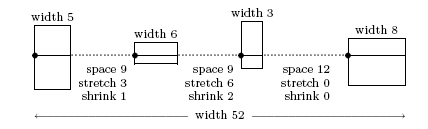
\includegraphics[width=0.9\linewidth]{./images/glue.png}
  \caption{Glue in \TeX}
  \label{fig:glue}
\end{figure}


\section{How to specify glue}

The usual way to specify \textit{glue} to \tex is
$<dimen>< plus~dimen><minus~dimen>$

where the plus and minus are optional and assumed to be zero if not
present; plus\index{glue!plus} introduces the amount of stretchability\index{glue!stretchability}, minus introduces the amount of shrinkability \index{glue!shrinkability}. 

For example, Appendix B of the TexBook defines \cs{medskip} to be an abbreviation for
|\vskip6pt plus2pt minus2p|. The normal-space component of glue must always be
given as an explicit dimen, even when it is zero. The ability of \TeX to stretch and shrink this glue has given it its beautiful looks. Strangely enough, although the algorithm is public it has not been used widely in other software.



\subsection*{hfil and hfill}

{\obeylines
{This text will be flush left.\hfil}
{\hfil This text will be flush right.}
{\hfil This text will be centered.\hfil}
{Some text flush left\hfil and some flush right.}
{Alpha\hfil centered between Alpha and Omega\hfil Omega}
{Five\hfil words\hfil equally\hfil spaced\hfil out.}
}

Consider the following definitions:

\begin{verbatim}
\def\centerlinea#1{\hfil#1\hfill}
\def\centerlineb#1{\hfill#1\hfill}
\def\centerlinec#1{\hss#1\hss}
We define quickly a \cs{lineX}\footnote{Strange but my \LaTeX\ distribution has not got on. (This definition is from \texttt{plain.sty}}

\def\lineX{\hbox to\hsize}
\def\lineX{\hbox to\hsize}
\def\centerlinea#1{\hfil#1\hfil}
\def\centerlineb#1{\hfill#1\hfill}
\def\centerlinec#1{\hss#1\hss}

\lineX{\centerlinea{\test}}
\lineX{\centerlineb{\test}}
\lineX{\centerlinec{\test}}
\centerline{\test}
\begin{center}\test\end{center}

\end{verbatim}


\section{Specifying glue amounts}

\tex glue is specified as a fixed dimension, and optionally, with a plus and
or minus dimension. Along with \cs{dimen} registers, TEX has glue registers,
called \cs{skip0} through \cs{skip255}. Here is how you can save glue settings in
\tex registers, and ask \tex to display the contents of one of them:

\begin{teX}
\skip1 = 10pt
\skip2 = 10pt plus 3pt
\skip3 = 10pt minus 2pt
\skip4 = 10dd plus 3dd minus 2dd
\the \skip4
\end{teX}


\texttt{> 10.70007pt plus 3.21002pt minus 2.14001pt}

The four sample glue settings store, respectively, {\em fixed glue}, {\em  stretchable
glue}, {\em shrinkable glue}, and {\em flexible glue}  that can both stretch and shrink,
but only up to a specified amount. Interword and intersentence spaces are
generally defined with glue like this, so that if more stretch or shrink of  a
re underfull (too little text to fill the line), or overfull (too much text in the
line).



\section{Overfull lines}

Although overfull lines are reported in the \tex log file, they can be hard
to find in the typeset document if they only stick out a little. To make
them highly visible while you are fine tuning your final document, assign
the variable \cs{overfullrule} a nonzero dimension, such as 2 cm. \tex then
displays a solid black box, called a \emph{rule}, of that width in the right margin
on each line that is overfull. Using the \docpkg{microtype} package one can adjust the parameters to minimize this.

To make the rules disappear, simply remove it,
or comment out, the assignment, or reset its value to 0 pt. 

Just as you can assign dimension registers to count registers to convert
from points to scaled points, you can assign skip registers to dimension and
count registers to discard the flexible parts:


\begin{teX}
\skip1 = 10pt plus 3pt minus 2pt
\the\skip1
 \dimen1 = \skip1
\the \dimen1
\count1 = \skip1
\the \count1
\end{teX}




\section{More on glue in boxes}

Besides normal glue with fixed amounts of stretch and shrink, \tex also has
two kinds of glue that are \emph{infinitely} stretchable and shrinkable: \cs{hfil} and
\cs{hfill} in horizontal mode, and \cs{vfil} and \cs{vfill} in vertical mode. Notice that there two versions
of the commands, the one ends with one ell and the second one with two. The
two-ell forms are more flexible than the one-ell forms.

The boxes and glue model is powerful, and \tex's author, Donald Knuth,
has written that he views it as the key idea that he discovered when he
first sat down in 1977--1978 to design a computer program for typesetting.
For example, to set something flush left, put infinitely-stretchable glue on
its right. To set it flush right, put the glue on the left. For centered material,
put the glue on both sides. Here are four examples, with vertical
bars marking the ends of the horizontal box (boxes have no visible frames,
although it is possible to write \tex commands to give them such outlines,
and we use that feature shortly):





\section{Horizontal and vertical boxes}


\noindent \lettrine{L}{ike} their dimensions \TeX's boxes are not what one thinks when thinking of boxes. TeX's boxes come in basically two flavours, horizontal boxes and vertical boxes. An \cs{hbox} is created by the command |\hbox{material}|. It has the following properties:

\begin{enumerate}
\item The material is placed from left to right and it becomes a \textit{horizontal list}.\index{horizontal list}
\item The box \textbf{cannot be broken across lines}; it is an indivisible unit.
\end{enumerate}

An |hbox| can contain, characters, horizontal glue, horizontal leaders or other boxes. While in many cases these other boxes can be other |\hbox|es, |\vbox| can be used.

Boxes can be moved up or down using |\raise| or |\lower|. Each of these primitives is followed by a dimension indicating how far the box can be lowered or raised.

Other material that can go in an hbox, is \textbf{vertical rules}. 

\subsection{The null macro}

The |\null| macro is defined both in Plain as well as LaTeX and generates an empty box. Its definition is:

\begin{teXXX}
\def\null{\hbox{}}
\end{teXXX}


\fbox{\hbox{This is a test}}

{
\fbox{\hsize=5cm
A test of a box at the end of a 2.0 inch line\par}

\fbox{\hsize=5.0cm in A test of a box at the end of a \hbox to 2cm{2.0 cm} line\par}

}

What happens when we have more than two boxes on a line? TeX will stuck them one under another. If they are enclosed within another hbox they will be inlined.



\begin{texexample}{}{}
\hbox to 1cm {A} \hbox to 1cm {B}

If we however, put them together in another |\hbox|, we get:

\hbox{\hbox to 1cm {A} \hbox to 1cm{B}}
\end{texexample}




An |\hbox| does not imply horizontal mode, so an attempt to start a paragraph with a box, for
instance
|\hbox to 0cm{\hss$\bullet$\hskip1em}Text ...|

will make the text following the box wind up one line below the box. It is necessary to switch
to horizontal mode explicitly, using for instance |\noindent| or |\leavevmode|. The latter is defined
using |\unhbox|, which is a horizontal command.


\begin{texexample}{}{}
\hbox to 0cm{\hss$\bullet$\hskip1em} Text ...


\leavevmode\hbox to 0cm{\hss$\bullet$\hskip1em} Text ...

\end{texexample}




\section{Kerning}

\begin{multicols}{2}
Using the command \cs{kern}, we can move boxes either left or right. Kerning is extensively used to build internal commands and we discuss it in more detail under the chapter for fonts.

Consider two horizontal boxes, holding the letters A and V:
As you can observe, the letters AB are a bit afar, from what would be a visually pleasant arrangement, we can kern them as follows:
\medskip
\begin{teXXX}
\hbox{\Huge AV A\kern-5ptV}
\end{teXXX}
\medskip
Note that hbox, does not produce a frame. I~have used a frame |\fbox|, which will cover a bit later as well as scaled the image by 2, in order to see the effects more clearly.
\columnbreak

\centerline{\scalebox{2}{\hbox{\hbox{\huge A}\hbox{\huge V}}} \scalebox{2}{\hbox{\hbox{\huge A}\kern-5pt\hbox{\huge V}}}}
\end{multicols}




\noindent\begin{tabular}{ll}
|\hbox{\kern4pt A\kern8pt B\kern8pt C\kern4pt}| & \fbox{\hbox{\kern4pt A\kern8pt B\kern8pt C\kern4pt}} \\
~ &\\
\midrule
|\hbox{\kern4pt\raise1pt\hbox{A}|  & \fbox{\hbox{\kern4pt\raise1pt\hbox{A} \kern8pt BC\kern8pt\lower6pt\hbox{D} \kern4pt} \kern8pt BC\kern8pt\lower6pt\hbox{D}\kern4pt} \\
|\kern8pt BC|                      &\\
|\kern8pt\lower6pt\hbox{D}|        &\\
|\kern4pt}|                        &\\ 
|\kern8pt BC|                      &\\ 
|\kern8pt\lower6pt\hbox{D}|        &\\
|\kern4pt}| &\\
\midrule
\end{tabular}


\vbox{
\noindent\rule{\linewidth}{0.4pt}
\begin{minipage}{4.5cm}
 \begin{teXX}
\fbox{\hbox{\kern4pt A\kern8pt 
      B\kern8pt C\kern4pt}}
\end{teXX}
\end{minipage}
\hfill\hfill
\begin{minipage}{3cm}
\hfill\hfill\fbox{\hbox{\kern4pt A\kern8pt 
      B\kern8pt C\kern4pt}}
\end{minipage}

\medskip
\noindent\rule{\linewidth}{0.4pt}
}

Notice that an |\hbox| is constructed by setting its components side by side so that their \textit{baselines} are aligned. When \cs{raise}, \cs{lower} are used the baselines are no longer aligned. In such a case the baseline of the box is defined as the baseline shared by the components before any vertical movements. In the example above the box now has a depth, as a result of lowering |D|.


\vbox{
\noindent\rule{\linewidth}{0.4pt}
\begin{minipage}{4.5cm}
\begin{teXXX}
\hbox{\kern4pt\raise1pt\hbox{A} 
  \kern8pt BC\kern8pt
  \lower6pt\hbox{D} 
  \kern4pt} 
\end{teXXX}
\end{minipage}
\hfill
\begin{minipage}{3cm}
\fbox{\hbox{\kern4pt\raise1pt\hbox{A} 
\kern8pt BC\kern8pt\lower6pt\hbox{D} \kern4pt}}
\end{minipage}

\medskip
\noindent\rule{\linewidth}{0.4pt}
}

\clearpage

\begin{multicols}{2}
\noindent\textbf{Vertical boxes.}\quad A vertical box is build in a similar manner to that of a horizontal list, except it is composed of material in the \textit{vertical list}.
When horizontal boxes are added in the list, they are stuck on top of each other as shown in the example below. 
\medskip
\begin{teXXX}
\vbox{\hsize=0.8cm\hbox{A} \hbox{AB}} 
\end{teXXX}
\columnbreak

\parindent0pt
\fbox{\vbox{\hsize=3cm\fbox{\hbox{ABCDEFGH}} \fbox{\hbox{AB}}}}
\end{multicols}

\begin{multicols}{2}
It is important to remember the two main differences between hboxes and vboxes. An hbox will expand to hold its material. If it need be it will overfill the line and produce an overful warning. A vbox will expand to hold its material. It is perfectly normal for a vbox to hold paragraphs, as shown. This is not possible with an hbox.

\columnbreak

\noindent\fbox{\vbox{\lorem\par\lorem\par}}
\end{multicols}



\topline
\begin{multicols}{2}
\noindent\textbf{Controlling the size of a vbox.}\quad What controls the size, is the containing environment. This in TeX, is specified using |\hsize|. In LaTeX this is controlled by an enclosing environment, maybe a minipage (which is build this way) or one of the page width parameters.
\end{multicols}



\begingroup
\parindent0pt
\fboxsep5pt
\hsize=3.8cm\footnotesize
\hfil\fbox{\vbox{\lorem\par}} 
\hfil\fbox{\vbox{\lorem\par}}
\hfil\fbox{\vbox{\lorem\par}}\hfill
\endgroup
\captionof{figure}{Output to demonstrate the use of vboxes.}


\begin{multicols}{2}
The code to typest the boxes shown above follows:
\medskip
\emphasis{hsize}
\begin{teXXX}
\bgroup
\parindent0pt
\hsize=3.3cm\footnotesize
\hfil\fbox{\vbox{\lorem\par}} 
\hfil\fbox{\vbox{\lorem\par}}
\hfil\fbox{\vbox{\lorem\par}}
\hfill
\egroup
\end{teXXX}
\columnbreak

Note, the use of hsize. We define the font size as |\footnotesize|. We have done this in order not to have overfull boxes--Latin words don't have a full set of hyphenation patterns in \latex. The macro |\lorem|, we have defined internally for this document. We place the code in a group in order not to affect the rest of the document.
\end{multicols}


\clearpage

\noindent\textbf{Vertical centering}\quad can be achieved by applying vertical infinite glue \cs{vfill}. In the example that follows, first we place two letters in individual |\hboxes| and we enclose them in a vbox. We apply |\vfill| both on top and at bottom.

\emphasis{\vfill}

\vbox{
\noindent\rule{\linewidth}{0.4pt}
\begin{minipage}{5cm}
\begin{teX}
\fbox{\vbox to 0.9cm{\vfil\hbox{M}\nointerlineskip\hbox{i}\vfil}} 
\end{teX}
\end{minipage}
\hfill
\begin{minipage}{3cm}
\hfill\fbox{\vbox to 0.9cm{\vfil\hbox{M}\nointerlineskip\hbox{i}\vfil}}\hfill\hfill 
\end{minipage}

\medskip
\noindent\rule{\linewidth}{0.4pt}
}



A |\vbox| can be combined with text and may appear anywhere within a paragraph. The baseline of the box will be aligned with the baseline of the current line.


\vbox{%
\noindent\rule{\linewidth}{0.4pt}}

\begin{teX}
A vbox can be placed within a paragraph \fbox{\vbox to 0.6cm{\vfil\hbox{M}\nointerlineskip\hbox{i}\vfil}} as shown here.


\hfill

A vbox can be placed within a paragraph \fbox{\vbox to 0.6cm{\vfil\hbox{M}
  \nointerlineskip\hbox{i}\vfil}} as shown here.

\end{teX}

\medskip
\noindent\rule{\linewidth}{0.4pt}






\noindent\textbf{Top alignment.}\quad\cs{vtop} is similar to a |\vbox|. The depth of this box is zero, since both A and B are capital letters. The width of this box is |\hsize|, since it contains text. 


\begin{codeexample}[]
\vtop{\hbox{A} \hbox{B}}
\end{codeexample}






Centering a picture in a box, both vertically and horizontally can be achieved using the methods we described so far.


\emphasis{hfill,hbox}
\begin{texexample}{}{}
     \fbox{%
          \vtop{\medskip
                    \hfill
                      \hbox{\includegraphics[width=1.5cm]{./images/amato.jpg}}%
                    \hfill 
                   \medskip%
                }%
      }%
\end{texexample}

\begin{texexample}{}{}
    \fbox{%
          \vtop{\medskip
                    \hfill
                      \hbox{\includegraphics[width=1.5cm]{./images/amato.jpg}}%
                      \hbox{\includegraphics[width=1.5cm]{./images/amato.jpg}}%
                      \hbox{\includegraphics[width=1.5cm]{./images/amato.jpg}}%    
                    \hfill 
                   \medskip%
                }%
      }%
\end{texexample}

Study the example a bit more carefully, as we have said earlier on that \cs{hbox}'es are stacked vertically, the reason why in the above example they are next to each other is that they are in an
\cs{fbox} which in turn is an \cs{hbox}  that can draw  frame around the box and is defined in the
\latex2e kernel.

So if we had only three images in hboxes we will get:

\begin{texexample}{Three Images Lined}{}
\leavevmode
\parindent30pt
\hbox{\includegraphics[width=1.5cm]{./images/amato.jpg}}%
\hbox{\includegraphics[width=1.5cm]{./images/amato.jpg}}%
\hbox{\includegraphics[width=1.5cm]{./images/amato.jpg}}%
\end{texexample}

\begin{macro}{\kern}
If we wanted to add a bit of space between the horizontal images, we could use \cs{kern}
Kern again. This is from the book TeX for The Impatient page 157. You can use kern in math mode, but you cannot use the \texttt{mu} units. If you want to use \texttt{mu} units use \cs{mkern} instead.
\end{macro}

\begin{texexample}{}{}
   \fboxsep=0pt
   \fbox{%
          \vtop{\medskip
                    \hfill
                      \hbox{\includegraphics[width=1.5cm]{./images/amato.jpg}}\kern10pt
                      \hbox{\includegraphics[width=1.5cm]{./images/amato.jpg}}\kern10pt
                      \hbox{\includegraphics[width=1.5cm]{./images/amato.jpg}}%    
                    \hfill 
                   \medskip%
                }%
   }%
\end{texexample}

\begin{texexample}{}{}
   \HHUGE
   \fboxsep=0pt
   \fbox{%
          \vtop{\medskip
                    \hfill
                       \hbox{ H\kern10pt i\kern10pt j}%    
                       \hbox{ A\kern10pt C\kern10pt j}%
                    \hfill 
                   \medskip%
                }%
   }%
\end{texexample}

This example shows how letters are typeset and you can see that they are aligned at the baseline. They are no different than the eimage example that we have shown earlier, except we don't need the boxes.

\medskip

\vbox{
\noindent\rule{\linewidth}{0.4pt}
\begin{minipage}{4.9cm}
\begin{teX}
\centerline{$\Downarrow$}\kern 3pt%
\centerline{$\Longrightarrow$\kern 6pt% horizontal kern
  \textit{A note about kern}\kern 6pt
    $\Longleftarrow$}
\kern 3pt
\centerline{$\Uparrow$}  
\end{teX}
\end{minipage}
\hspace{0.3cm}
\begin{minipage}{4.5cm}
\centerline{$\Downarrow$}\kern 3pt%
\centerline{$\Longrightarrow$\kern 6pt% horizontal kern
  \textit{A note about kern}\kern 6pt
    $\Longleftarrow$}
\kern 3pt
\centerline{$\Uparrow$}
\end{minipage}

\medskip
\noindent\rule{\linewidth}{0.4pt}
}
\medskip

To make a point again, |\vbox| lines boxes at their bottom while, |\vtop| lines them at their top.

\medskip

\vbox{
\noindent\rule{\linewidth}{0.4pt}
\begin{minipage}{4.9cm}
\begin{teX}
 \hbox{\hsize=2cm \raggedright
\vbox to 0.5in{\hrule This box is .5in deep. \vfil\hrule}
\qquad
\vbox to 0.75in{\hrule This box is .75in deep. \vfil\hrule}
\qquad
\end{teX}
\end{minipage}
\hspace{0.3cm}
\begin{minipage}{4.5cm}
\hbox{\hsize=2cm \raggedright
\vbox to 0.5in{\hrule This box is .5in deep. \vfil\hrule}
\qquad
\vbox to 0.75in{\hrule This box is .75in deep. \vfil\hrule}
\qquad}
\end{minipage}

\medskip
\noindent\rule{\linewidth}{0.4pt}
}

\medskip


Trying the same with vtop

\medskip

\vbox{
\noindent\rule{\linewidth}{0.4pt}
\begin{minipage}{4.9cm}
\begin{teX}
 \hbox{\hsize=2cm \raggedright
\vbox to 0.5in{\hrule This box is .5in deep. \vfil\hrule}
\qquad
\vbox to 0.75in{\hrule This box is .75in deep. \vfil\hrule}
\qquad
\end{teX}
\end{minipage}
\hspace{0.3cm}
\begin{minipage}{4.5cm}
\hbox{\hsize=2cm \raggedright
\vtop to 0.5in{\hrule \smallskip This box is .5in deep. \vfil\hrule}
\qquad
\vtop to 0.75in{\hrule \smallskip This box is .75in deep. \vfil\hrule}
\qquad}

\hbox{\hsize=2cm \raggedright
\vbox to 0.5in{\hrule \smallskip This box is .5in deep. \vfil\hrule}
\qquad
\vbox to 0.75in{\hrule \smallskip This box is .75in deep. \vfil\hrule}
\qquad}
\end{minipage}

\medskip
\noindent\rule{\linewidth}{0.4pt}
}

\medskip

There are some other special macros defined by Plain TeX that we will only touch briefly here. One of them is \cs{underbar}{\index{Plain!\textbackslash underbar}.
The macro puts its argument into an hbox and underlines it.

\medskip

\vbox{
\noindent\rule{\linewidth}{0.4pt}
\begin{minipage}{4.9cm}
\begin{teX}
 \underbar{1,000,788.22}
\end{teX}
\end{minipage}
\hspace{0.4cm}
\begin{minipage}{4.0cm}
\medskip
\hfill\hfill{}\hspace*{1em}a1,000,700.22 \hfill

\smallskip

\hfill\underbar{1,000,788.22}\hfill
\end{minipage}

\medskip
\noindent\rule{\linewidth}{0.4pt}
}

\medskip


The \cs{everyvbox} command inserts a series of tokens at the beginning of every |\vbox|.


\medskip

\vbox{
\noindent\rule{\linewidth}{0.4pt}
\begin{minipage}{4.9cm}
\begin{teX}
 \everyvbox{$\bullet$}...
\end{teX}
\end{minipage}
\hspace{0.4cm}
\begin{minipage}{4.0cm}
\begingroup% Without this group, there are tons of problems!
   \everyvbox{$\bullet$}
   \global\setbox1=\vbox{This is a paragraph without an initial indent. It is   \the\hsize\ long lines.}
   \global\setbox2=\vtop{\copy1}
\endgroup
 \hbox{\box1} 

 \hbox{\box2}
\end{minipage}

\medskip
\noindent\rule{\linewidth}{0.4pt}
}

\medskip
Knuth in the TexBook Chapter 24, has some short description of the every commands. The `everyhbox` inserts a token list just before as its name implies a horizontal box.

Here is a short example. We define a `oneLineBox`, which is simply an hbox with some text and we add spread to spread the line. Using |\everybox| we add the letter \textbf{a} in each horizontal box. 


\tex considers the box overfull if the excess width of the box is larger than \cs{hfuzz} or \cs{hbadness} is less than 100. If I change  the badness to hbadness, I get 1000.

\medskip

\vbox{
\noindent\rule{\linewidth}{0.4pt}
\begin{minipage}{10.0cm}
\begin{teX}
 \begingroup
     \everyhbox{a}
     \def\oneLineBox#1#2%
     {%
          \hfuzz=0pt
          \overfullrule=0.25pt
          \setbox0=\hbox spread#2{#1}%
          \setbox1=\hbox{\the\badness}% 
          \setbox2=\hbox to 4.5cm{\box0\hfil\box1}%
          \box2
     }
     \oneLineBox{Badness of line }{-1em}
     \oneLineBox{Badness of line }{-0.54em}
     \oneLineBox{Badness of line }{-0.4em}
     \oneLineBox{Badness of line }{0em}
     \oneLineBox{Badness of line }{1em}
     \oneLineBox{Badness of line }{2em}
     \oneLineBox{Badness of line }{3em}
 \endgroup
\end{teX}
\end{minipage}


\begin{minipage}{10.0cm}
\begingroup
     \everyhbox{a}
     \def\oneLineBox#1#2%
     {%
          \hfuzz=0pt
          \overfullrule=0.25pt
          \setbox0=\hbox spread#2{#1}%
          \setbox1=\hbox{\the\badness}% 
          \setbox2=\hbox to 4.5cm{\box0\hfil\box1}%
          \box2
     }
     \oneLineBox{Badness of line }{-1em}
     \oneLineBox{Badness of line }{-0.54em}
     \oneLineBox{Badness of line }{-0.4em}
     \oneLineBox{Badness of line }{0em}
     \oneLineBox{Badness of line }{1em}
     \oneLineBox{Badness of line }{2em}
     \oneLineBox{Badness of line }{3em}
 \endgroup
\end{minipage}

\medskip
\noindent\rule{\linewidth}{0.4pt}
}

\medskip



















\section{More features of horizontal boxes}

Characters in the Latin alphabet have different shapes, and in most typefaces,
different widths. The letters \texttt{d f h k l t} have ascenders, making them
higher than the vowels \texttt{a e o u}, while the letters \texttt{f g j p q y} have descenders,
giving them added depth below the vowels. Similarly, an \texttt{m} is wider than
an \texttt{i}. 

When \tex makes a normal horizontal box, the box width is the sum
of the widths of the characters, and the fixed parts of any glue, contained
in it. Shrink and stretch components of glue are discarded for the width
calculation. The box also has both a height above the baseline, the invisible
line on which the characters rest, and a depth below the baseline. The
depth is zero if there are no objects with descenders. The height and depth
are chosen from the largest vertical extents of the contained objects.

If you look carefully at typeset material, you will observe that, in most
typefaces, parentheses, brackets, and braces have both descenders and ascenders,
and the typeface designer usually makes their extents the maximum
among all of the characters in the design. This sample text shows
document: ( h g ) [ k j ] { l p }.

You can force TEX to choose a larger height and depth than normal when
you write a command for a horizontal box by ensuring that it has suitable
contents, such as an invisible vertical rule of zero width. The command

\verb+\hbox to 50pt {\vrule height 20pt depth 10pt width 0pt \it stuff}+

produces a box whose (invisible) outline looks like this: 

\hbox to 50pt {\vrule height 20pt depth 10pt width 0pt \it Great}

\noindent\fbox{\vrule height 20pt depth 10pt width 0pt \it Great}




The
three extents of the vertical rule can appear in any order, and any convenient
units.

\section{LaTeX Boxes}
In order to see the otherwise-invisible box edges in that example, we
used the \latex  built-in command \cs{fbox} to create a frame, and we eliminated
the default margin inside the frame by setting \cs{fboxsep = 0pt}. Plain TEX
does not have the \cs{fbox} command, but The TEXbook shows how to make
something like it on pp. 223 and 321.

One particular zero-width vertical rule is convenient for ensuring that
separate boxes all get the same height and depth. It has the height and
depth of parentheses in the normal prose font, and is given the macro name
\doccmd{strut}. Its definition in the plain.tex file of macro definitions is roughly
equivalent to this:

\begin{comment}
\begin{figure}[tbp]%
   \includegraphics[width=\linewidth]{./graphics/ascender.jpg}
   \caption{Boxes in \protect\TeX}
   \label{fig:ascender}
\end{figure}
\end{comment}

 \def \strut {\vrule height 8.5pt depth 3.5pt width 0pt}
\begin{teX}
  \def \strut {\vrule height 8.5pt depth 3.5pt width 0pt}
\end{teX}

Compare these two experiments with outlined boxes, first without struts,
and then with struts:




Notice the different vertical extents of the boxes in the first case, and how
they have identical extents in the second case.

\section{Horizontal alignment of boxes in TEX}

When horizontal boxes are set together, they are treated as separate words,
and therefore spaced accordingly. The input

\verb+ \fbox{one} \fbox{two} \fbox{three}\fbox{four}+  

produces  \fbox{one} \fbox{two} \fbox{three}\fbox{four}. As the example shows, we can put spaces
between them, or run them together so that they fit tightly.


\section{Vertical boxes in TEX}


\begin{minipage}{2.0in}
\begin{verbatim}
\noindent
\fbox{%
  \it
  \hbox to 80pt{%
     \parindent = 0pt
     \vbox to 30pt {%
         left text
         \vfil
         more left text%
     }%
  }%
}%
\end{verbatim}
\end{minipage}


%\noindent
\fbox{%
  \it
  \hbox to 80pt{%
     \parindent = 0pt
     \vbox to 30pt {%
         left text
         \vfil
         more left text%
     }%
  }%
}%

Firstly we use a noindent to ensure that the box is not indented. If you comment the\cs{fbox} out, you can see that the right amount of space has been left in the paragraph above.

\mbox{}
 
\noindent
\fbox{%
\it
\hbox to 80pt{%
\parindent = 0pt
\hsize = 80pt
\vbox to 30pt {\hfill right text
\vfil
\hfill more right text}
}%
}%



\noindent
\fbox{%
\it
\hbox to 80pt{%
\parindent = 0pt
\hsize = 80pt
\vbox to 30pt {\hfil center text
\vfil
 more center text \hfil}
}%
}%

We can aslo center the text for both lines, by modifying the code slightly.
\begin{teX}
\noindent
\fbox{%
\it \hbox to 80pt{
   \parindent = 0pt
   \hsize = 80pt
   \vbox to 30pt {
   center text \hfill
    \vfil
    \hfil more center text}
   }%
}%
\end{teX}


\noindent
\fbox{%
\it
\hbox to 80pt{%
\parindent = 0pt
\hsize = 80pt
\vbox to 30pt {\hfil center text
\vfil
\hfil more center text}
}%
}%



\chapter{Boxes with \protect\LaTeXe}

A  box of specified width is provided in \latex with the command:

\cs{makebox}\oarg{width}\oarg{position}\marg{contents}. 

The source2e manual states. If the width is missing, then position is also missing and obj  is put in an \cs{hbox} of its natural width. This is true as far as the looks are concerned, but not the behaviour, as you can see
from the following example is not an unqualified hbox it is an hbox preceded by leavevmode.\footnote{\url{http://tex.stackexchange.com/questions/105585/latex2e-makebox-hbox}} This is of course good practice and brings consistency to the LaTeX kernel. I would recommend that you follow such practices in your own code. 

\begin{texexample}{}{}
\newbox\temp
\savebox\temp{test}
LaTeX

\makebox{test} \mbox{test}

TeX

\hbox{test} \hbox{test}

\indent\hbox{test} \hbox{test}

LaTeX with \cs{leavemode}

\makeatletter
\leavevmode\hbox to \wd\temp{test} \indent\hbox to \wd\temp{test}
\makeatother
\end{texexample}



\latex's analog of a\cs{hbox} is called \cs{mbox}. They are 
much the same thing, but \cs{mbox} is defined to be more widely usable. We have already used \latex's framed companion to \cs{mbox}, \cs{fbox}.

A horizontal box of specified width is provided in \latex with the command
\doccmd{makebox[width][position]\{contents\}}. Bracketed command arguments
in \latex are always optional. 

Here, the width is a TEX dimension,
and defaults to the natural width of the contents if not given. The position
is one of the letters \textbf{l} (flush left) or \textbf{r} (flush right); if it is omitted, the text
is centered in the box. If the specified width is smaller than needed, the
contents protrude from the box, and may overlap surrounding material. If
the specified width is zero, then we have equivalents of the TEX \cs{rlap} and
\cs{llap} commands.


Here are several examples of these three LATEX box commands:

{\obeylines
\mbox{stuff}

\fbox{stuff} 

|\makebox{stuff}|

|\makebox[40pt][l]{stuff}|

|\makebox[40pt][r]{stuff}|

|\makebox[0pt]{stuff}|

|\makebox[0pt][l]{stuff}|

|\makebox[0pt][r]{stuff}|
}


The \cs{makebox} command has a framed companion, \cs{framebox}, with identical
arguments. Like \cs{fbox}, \cs{framebox} creates a margin of width \cs{fboxsep}
between the outline and the contents, but we continue with a zero value for
that separation:



\framebox{stuff} 

\framebox[40pt][l]{stuff} 

\framebox[40pt][r]{stuff}

\framebox[0pt]{stuff} 

\framebox[0pt][l]{stuff} 

\framebox[0pt][r]{stuff}

The last three examples show that the frame shrinks to a vertical bar when
the box width is zero.

To help in positioning boxes within other objects, \latex provides the command
\cs{raisebox} to raise and lower boxes:

\begin{teX}
\raisebox{raiselength}[height][depth]{contents}
\end{teX}

A negative first argument lowers the box. Here are some examples:


A \raisebox{10pt}{\fbox{upper}} A
upper
A \raisebox{10pt}{\
fbox{lower}} A
lower
A \fbox{\raisebox{10pt}[25pt]{\fbox{upper}}} A
upper
A \fbox{\raisebox{10pt}[
25pt]{\fbox{lower}}} A
lower
A \fbox{\raisebox{10pt}[25pt][15pt]{\fbox{upper}}} A
upper
A \fbox{\raisebox{10pt}[
25pt][15pt]{\fbox{lower}}} A
lower

\section{Paragraph Boxes}

\begin{macro}{\parbox}
For longer strings of text, \latex provides the paragraph box \cs{parbox}, which is
defined like this: 
\end{macro}
\medskip
\cs{parbox}\oarg{position}\oarg{height}\oarg{innerpos}\marg{width}\marg{contents} 
\medskip

The optional position
is a letter \textbf{b} for alignment of the bottomline with the current baseline,
or \textbf{t} for alignment of the top line with the surrounding baseline. Without

The box can be used as if it were a letter or a word, so we can put it in
the middle of a sentence. The input

This is text \parbox{30pt}{\it and this is boxed text} and
this is more text.

This is text \fbox{\parbox{30pt}{\it and this is boxed text}}
and this is more text.
produces


Flush-right typesetting generally looks bad in narrow columns, so we
can insert a \cs{raggedright} command inside the last argument of the paragraph
box to get output like this:

\begin{texexample}{}{}

\parbox[b][120pt][t]{100pt}{\lorem}%
\hspace{1cm}%
\parbox[b][120pt][t]{100pt}{Only some short line of text here.}%



\parbox[b][100pt][t]{100pt}{\lorem}\hspace{1cm}\parbox[b][100pt][c]{100pt}{Only some short line of text here.}

\end{texexample}


\section*{The minipage environment}

Another kind of paragraph box can be obtained in a more general, and
more powerful, way with the minipage environment:

\begin{teX}
\begin{minipage}[position]{width}
   contents
\end{minipage}
\end{teX}


The positioning works just like that for \verb+ \parbox+, with alignment letters b
and t, and if they are omitted, a default of vertical centering.
In particular, verbatim text produced with the verb command is illegal
in macro arguments, so it cannot be used with \cs{fbox}, \cs{framebox}, \cs{makebox},
\cs{mbox}, or\cs{ parbox}, but it can be used inside a minipage. The input


\begin{texexample}{}{}
\begin{minipage}{170pt}
This is inline verbatim \verb=\verb|\%{}|=, and this
is a verbatim display:

\begin{verbatim}
#include <stdio.h>
#include <stdlib.h>
int main(void)
{
  printf("Hello, world\n");
  exit (EXIT_SUCCESS);
}
\end{verbatim}
\end{minipage}

\end{texexample}


A minipage can go everywhere and can hold virtually any content.





\section{Scaling and resizing boxes}

The command \cs{resizebox}\marg{width}\marg{height}\marg{object} can be used with tabular to specify the height and width of a table. The following example shows how to resize a table to 8cm width while maintaining the original width/height ratio.

\begin{teX}
\resizebox{8cm}{!} {
  \begin{tabular}...
  \end{tabular}
}
\end{teX}

Alternatively you can use \cs{scalebox}{ratio}{object} in the same way but with ratios rather than fixed sizes:

\begin{teX}
\scalebox{0.7}{
  \begin{tabular}...
  \end{tabular}
}
\end{teX}

Both |\resizebox| and |\scalebox| require the \docpkg{graphicx} package.
To tweak the space between columns (LaTeX will by default chose very tight columns), one can alter the column separation: |\setlength{\tabcolsep}{5pt}|. The default value is |6pt|.

The scalebox is great if you want to magnify a letter so that you can observe the design closer.

\bigskip
\noindent\begin{tabular}{|c|c|c|c|c|c|}\hline
Kp-Fonts & Kp-\textit{light} & CM & Palatino & Utopia & Times\\\hline\hline
\scalebox{2}{ag713} &
\scalebox{2}{\fontfamily{jkpl}\selectfont 7} &
\scalebox{2}{\fontfamily{lmr}\selectfont 713}  &
\scalebox{2}{\fontfamily{ppl}\selectfont 713}  &
\scalebox{2}{\fontfamily{put}\selectfont 7} &
\scalebox{2}{\fontfamily{ptm}\selectfont \oldstylenums{7}} \\\hline
\end{tabular}


\begin{teX}
\hspace{-6mm}\begin{tabular}{|c|c|c|c|c|c|}\hline
Kp-Fonts & Kp-\textit{light} & CM & Palatino & Utopia & Times\\
\hline\hline
  \scalebox{10}{a} &
  \scalebox{10}{\fontfamily{jkpl}\selectfont a} &
  \scalebox{10}{\fontfamily{lmr}\selectfont a}  &
  \scalebox{10}{\fontfamily{ppl}\selectfont 7}  &
  \scalebox{9.2}{\rule{0pt}{1.25ex}\fontfamily{put}\selectfont a} &
  \scalebox{10}{\fontfamily{ptm}\selectfont a}\\\hline
\end{tabular}
\end{teX}
\bigskip



















\makeatletter \cxset{toc image = \@empty}
\chapter{GROUPING AND SCOPING RULES}
\index{Grouping}
\label{ch:grouping}

Like most computer languages \tex\ has a grouping mechanism that is able to confine most changes to a particular locality. This chapter explains what sort of actions can be local, and how groups are formed.
\medskip

\DescribeMacro{\bgroup}
       Implicit beginning of group character.

\DescribeMacro{\egroup} Implicit end of group character.

\DescribeMacro{\begingroup} Open a group that must be closed with |\endgroup|.

\DescribeMacro{\endgroup} Close a group that was opened with |\begingroup|.

\DescribeMacro{\aftergroup} Save the next token for insertion after the current group ends.

\DescribeMacro{global} Make assignments, macro definitions, and arithmetic global.

\DescribeMacro{globaldefs} Parameter for overriding |\global| prefixes. IniTEX default: 0.



The grouping mechanism can be thought of a bit like scope in other programming languages, with the
exception that in \tex the mechanism is much more Pascal-like. Most assignments made inside a group are local to that group
unless explicitly indicated otherwise, and outside the group old values are restored (pretty much like in Pascal). If we type the following  example:

\begin{texexample}{}{}
\def\i{42}
{
   \def\i{43}
   \def\b{2}
}
The value of the \textbackslash i is now \i

\def\x{a}
\let\y\x
\bgroup
  \def\x{b}
  Within group \x\par
\egroup
  Outside group \x
\end{texexample}

we get   \texttt{The value of the \textbackslash i is now 42}. Due to the way \tex scoping rules work, the old program state
will be restored \textit{completely} after returning from the local group. Neither the change to |\i| nor the definition of |\b| will survive. This is also true for register changes or other assignments.

The listing above defines |\i| enters a local scope (a \tex group) and changes |\i|

The |\end| command is allowed to occur inside a group, but TEX will give a diagnostic
message about this.

The \cs{aftergroup} control sequence saves a token for insertion after the current group. Several
tokens can be set aside by this command, and they are inserted in the left-to-right order in which
they were stated.

\begin{texexample}{}{}
\def\x#1;{#1}
\def\y{15}
{\globaldefs1
\bgroup
   \def\y{0}
   \aftergroup\x\aftergroup\y\aftergroup;
   \aftergroup}
\egroup
\y


\globaldefs0

\def\z{1}
{\def\z{0}
\z
}

\z

\end{texexample}

\begin{texexample}{}{}
{ \def\z{1}
  {\def\z{0}\globaldefs1
     \z
    {
	\z
    }
   \z
  }
 \z
}





\end{texexample}



\section{Local and global assignments}

An assignment or macro definition is usually made global by prefixing it with \cs{global}, but nonzero
values of the integer parameter |globaldefs| override |doccmd{global}|
is positive every assignment is implicitly prefixed with \doccmd{global}, and if |\globaldefs| is negative,
|\global| is ignored. Ordinarily this parameter is zero. It has very
limited use and even in the \latex\ kernel we can only find 3-4 uses when defining math fonts.


Some assignment are always global: the \marg{global} assignments are:

font assignment assignments involving \cs{fontdimen}, \cs{hyphenchar}, and \cs{skewchar}.

hyphenation assignmenti \cs{hyphenation} and \cs{patterns} commands.

hbox size assignmenti altering box dimensions with \cs{ht}, \cs{dp}, and \cs{wd} 

hinteraction mode assignmenti run modes for a \tex job (see Chapter 32).

hintimate assignmenti assignments to a hspecial integeri or hspecial dimeni;


\section{Braces}

The most common way to group is to use braces. They are used for two purposes:

\begin{enumerate}
\item to indicate the start and end of a group. For example |{\small here is some text}|.

\item to indicate that a string of tokens should be treated as one unit. For example in |\def\abc{...}| the braces are used
to delimit the argument.
\end{enumerate}

It is important to note that the characters \{, \} are not hardwired in \tex. Any tokens with catcodes 1 and 2 can be used.
The plain format starts [343] by saying:

\begin{teX}

\catcode`\{ =1
\catcode `} = 2
\end{teX}

Tokens with catcodes 1 and 2 are called \emph{explicit braces}. An \emph{implicit} brace is a control sequence whose replacement text is an explicit brace. Thus the two |plain| control sequences 
|\bgroup| and |\egroup| are implicit braces. They are defined in [353] by:

There is also a low-level \tex operator pair for creating groups. It works
just as the braces. A group is started with \cs{begingroup} and ended with
\cs{endgroup}. These operators may be freely mixed with braces but pairs
should be properly matched. So ��|{ \begingroup \endgroup }|�� is allowed
but ��|{ \begingroup } \endgroup|�� is not.

\begin{teX}
\let\bgroup={
let\egroup=}
\end{teX}

They can be used where unbalanced braces are needed.

Salomon gives an example to typeset a number of paragraphs with a negative indentation\footnote{This style can sometimes be found in old books.}:

\begin{teX}
\def\negIndent{\brgoup\parindent=-20pt}
\def\endIndent{\par\egroup}

\negIndent
  \small\lipsum[1]
\endIndent
\end{teX}

This will typeset:

\def\beginindent{\bgroup\parindent=-20pt}
\def\endindent{\par\egroup}

\beginindent
  \small\lipsum[1-3]
\endindent


The other two primitives \cs{begingroup} and \cs{endgroup} can also be used to define a group. However a group that starts with a |begingroup| must end with an |\endgroup|. This provides a mechanism for error checking, which \tex's parsing routines can easily catch.

Note that |\begingroup| and |\endgroup| can only be used to define a group, not to delimit a string. You can say:

\begin{teX}
\begingroup
  \it abc
\endgroup
\end{teX}

but the following will get \tex to complain about missing braces

\begin{teX}
\hbox\begingroup\it abc\endgroup
\end{teX}



\section*{Examples}
From the TexBook Exercise 7.4

Suppose that the commands
\begin{texexample}{}{}
{\catcode`\<=1 \catcode`\>=2
 \bfseries test
>
 test
\end{texexample}

appear near the beginning of a group that begins with |{| these specifications instruct
TEX to treat |<| and |>| as group delimiters. According to \tex's rules of locality, the
characters |<| and |>| will revert to their previous categories when the group ends. But
should the group end with |}| or with |>| ?

It ends with either |>| or |}| or any character of category 2; then the effects of all
\cs{catcode} definitions within the group are wiped out, except those that were global.
\tex  doesn't have any built-in knowledge about how to pair up particular kinds of
grouping characters. New category codes take effect as soon as a |\catcode| assignment
has been digested. For example,

\begin{teX}
{\catcode`\>=2 >
\end{teX}

is a complete group. But without the space after |2|  it would not be complete, since TEX
would have read the |>|  and converted it to a token before knowing what category code
was being specified; \tex always reads the token following a constant before evaluating
that constant.

\topline

\textbf{Example}: \textsc{Adjusting the spacing of a font} An interesting example that illustrates some of the concepts that were discussed so far is to try and change the \textit{inter word spacing} of text using the \cs{fontdimen2} parameter. The interesting aspect of this example is that
we want to change the spacing, but since the font changes are global, we want to revert back to the original font at the end of the group. Although there are many other ways of achieving this we will use the \cs{aftergroup}.

\begin{teX}
\font \roman=cmr10
\font\specroman=cmr10
%% Next, the special registers
\newdimen\savedvalue
\savedvalue=\fontdimen2\roman
\newdimen\specialvalue
\specialvalue=13.0pt
%% Finally, definitions.
\def \rm{%
  \fontdimen2\roman=\savedvalue }
\def\specrm{%
  \aftergroup\restoredimen
  \fontdimen2\specroman=\specialvalue
  \specroman  }
\def\restoredimen{%
\fontdimen2\roman=\savedvalue }
\end{teX}
{
%% First, fonts.
\font \roman=cmr10
\font\specroman=cmr10
%% Next, the special registers
\newdimen\savedvalue
\savedvalue=\fontdimen2\roman
\newdimen\specialvalue
\specialvalue=13.0pt
%% Finally, definitions.
\def \rm{%
  \fontdimen2\roman=\savedvalue }
\def\specrm{%
  \aftergroup\restoredimen
  \fontdimen2\specroman=\specialvalue
  \specroman  }
\def\restoredimen{%
\fontdimen2\roman=\savedvalue }


{\bf Spaced Out Text} 
\medskip
{\specrm \lorem} dimension2 the interword   value \the\fontdimen2\font


{\bf  Back to Normal}
\medskip

\rm
\lorem

}

This is a test \\{item}
\section{Summary}
\relax\bgroup\relax\egroup\relax 


\section*{Scoping Rules for boxes}

The scoping rules for boxes work similarly to those for other command sequences, since they are just macros defined by \latex or |plain|. In the example below, we define a box |\mybox| and we save a sentence both in global scope as well as local scope.

\begin{teX}
\documentclass{article}
\begin{document}
  \newsavebox{\mybox}
  \savebox{\mybox}{Outside scope}
  \usebox\mybox
  \begin{minipage}{5cm}
    \sbox{\mybox}{from first minipage}(*@ \label{global} @*)
    \usebox\mybox
  \end{minipage}
  \usebox{\mybox}
\end{document}
\end{teX}


This will typeset:
\medskip

\newsavebox{\myboxi}
\savebox{\myboxi}{\tt > Outside scope}

\noindent\usebox\myboxi

\noindent\begin{minipage}{5cm}
\sbox{\myboxi}{\tt > from first minipage}
\noindent\usebox\myboxi
\end{minipage}

\noindent\usebox{\myboxi}


\medskip 
Changing line [\ref{global}] to |\global\sbox| will make the definition of |\mybox| within the minipage environment global and would change the output to:
\medskip



To save memory space, box registers become empty by using them: \tex assumes
that after you have inserted a box by calling |\boxnn| in some mode, you do not need the contents of that register any more and empties it. In case you do need the contents of a box register more
than once, you can |\copy| it. Calling |\copynn| is equivalent to |\boxnn| in all respects except that the register is not cleared.


There are 256 box registers, numbered 0–255. Either a box register is empty (‘void’), or it contains
a horizontal or vertical box. This section discusses specifically box registers; the sizes of boxes,
and the way material is arranged inside them, is treated below.




\newbox\MyBox

\setbox\MyBox=\hbox{\hfil Test\hfill}

\unhbox\MyBox


\noindent\unhbox\MyBox

\noindent{\hfill Test \hfill}



\framebox{\parbox{\linewidth}{\color{black}
\textbf{\textcolor{purple}{\textsf{CAUTION}}}
\begin{enumerate}
\itemsep-5pt
\item \latex will not empty a box as it uses the copy command in the definition of the newsavebox.
\item It is better to use \LaTeX\ commands rather than \tex primitives, when defining boxes, as \latex tests for duplication of names - which is very important if a user uses a lot of different packages.
\item Give always preferences to local definitions rather than global. Globals always create maintenance problems in programming.
\end{enumerate}
}}


\section{Implicit Grouping}

There are  instances where grouping is \textit{implicit}. What this means is that \text starts and ends a group automatically and without any action by the user. There are two major cases where this happens:

\begin{enumerate}
\item The text inside a box such as |\hbox|, |\vbox|, |\vtop|, |\vcenter| etc. is automatically treated by \tex as a group.  For example |\hbox{\bf My Heading}|, will print  \hbox{\bf My Heading}  and it will not continue with the bold font once outside the group. All these commands have curly brackets and these curly brackets form implicit groups.
\item In five cases \tex forms implicit groups. In some of these cases not even curly braces are involved.
\end{enumerate}

\begin{enumerate}
\item The text inside math mode is treated as a group. This is true both for inline math as well as display math.
\item Matching |\left| and |\right| primitives treat the formula in between them as a group.
\item Fractions are treated as a group.
\item The execution of an ouput routine is implicitly enclosed in a group.
\item Columsn in |\halign| based tables are local.
\end{enumerate} 

\subsection{\texttt{afterssignment and grouping}}

The primitive |\afterasignment| does not follow grouping in that it does not save the definition of a token when |\afterassignment| is executed. Consider the following example:

Define the two macros |\xx| and |\yy|.

\def\xx{\string\xx\ executed\par }

\def\yy{\string\yy\ executed\par }

\afterassignment\xx

We start a group, where we have two definitions of |\xx| and |\yy|

{
  \def\xx{\string\xx executed inside a group\par}

  \def\yy{\string\yy executed inside a group\par}

The second afterassignment is execute

  \afterassignment\yy

The group is ended

}


Note afterassignment saves the token following afterassignment without expanding it. Nothing happens until after the next assignment; immediately after the next assignment the saved token is expanded. This is a bit of a tricky part and you can go over it to make sure you understand it well.



Assign a value or define a macro.





































\chapter{Poetry}

\epigraph{"Carpe diem. Seize the day, boys. Make your lives extraordinary."}{---John Keating, Dead Poets Society (1989)}

\newcommand{\garden}{
I used to love my garden \\
But now my love is dead \\
For I found a bachelor's button \\
In black-eyed Susan's bed.
}
Typographical standards require poetry to be `'centered on the longest line, unless such line is disproportionately long, in which case optical centring''. \textit{The oxford Dictionary for Writers and Editors}, which presents the house style of
the Oxford University Press). 


\section{Using the verse package}



\begin{lstlisting}[language={[common]TeX},% 
                           alsolanguage={[LaTeX]TeX},% 
                           alsolanguage={[primitive]TeX},%
                           alsolanguage={extras}]
\renewcommand{\poemtoc}{subsection}
\poemtitle{A Limerick}
\settowidth{\versewidth}{There was an old party of Lyme}
\begin{verse}[\versewidth]
    There was an old party of Lyme \\
    Who married three wives at one time. \\
    \vin When asked: `Why the third?' \\
    \vin He replied: `One's absurd, \\
    And bigamy, sir, is a crime.'
\end{verse}
\end{lstlisting}


which gets typeset as below. The default \doccmd{poemtoc}  is redefined to subsection so
the title is entered into the ToC as an unnumbered subsection.

\newlength{\aaaa}
\settowidth{\aaaa}{ZZZZ}

\renewcommand{\poemtoc}{subsection}
\poemtitle{A Limerick}
\settowidth{\versewidth}{There was an old party of Lyme}
\begin{verse}[\versewidth]
    There was an old party of Lyme \\
     Who married three wives at one time. \\
    \vin When asked: `Why the third?' \\
    \ZZZZ He replied: `One's absurd, \\
And bigamy, sir, is a crime.'
\end{verse}

Next is the Garden verse within the altverse environment. It is titled and
centered.

\settowidth{\versewidth}{But now my love is dead}
\poemtitle{Love's lost}
\begin{verse}[\versewidth]
\begin{altverse}
\garden
\end{altverse}
\end{verse}


which produces:

\settowidth{\versewidth}{But now my love is dead}
\poemtitle{Love's lost}
\begin{verse}[\versewidth]
    \begin{altverse}
    \garden
\end{altverse}
\end{verse}


It is left up to you how you might want to add information about the author
of a poem. Here is one example of a macro for this:

\begin{lstlisting}[language={[common]TeX},% 
                           alsolanguage={[LaTeX]TeX},% 
                           alsolanguage={[primitive]TeX},%
                           alsolanguage={extras}]
\newcommand{\attrib}[1]{%
\nopagebreak{\raggedleft\footnotesize #1\par}}
\end{lstlisting}

\newcommand{\attrib}[1]{%
\nopagebreak{\raggedleft\footnotesize #1\par}}
This can be used as in the next bit of doggeral.

\poemtitle{Fleas}
\settowidth{\versewidth}{What a funny thing is a flea}
\begin{verse}[\versewidth]
What a funny thing is a flea. \\
You can't tell a he from a she. \\
 But he can. And she can. \\
 Whoopee!
\end{verse}
\attrib{Anonymous}


Here is an example of line wrapping.
\poemtitle{In the beginning}
\settowidth{\versewidth}{And objects at rest tended to remain at rest}
\begin{verse}[\versewidth]
Then God created Newton, \\*
And objects at rest tended to remain at rest, \\*
And objects in motion tended to remain in motion, \\*
And energy was conserved
and momentum was conserved
and matter was conserved \\*
And God saw that it was conservative.
\end{verse}
\attrib{Possibly from \textit{Analog}, circa 1950}



Here is one with a forced line break and a slightly different title style.

\begin{lstlisting}[language={[common]TeX},% 
                           alsolanguage={[LaTeX]TeX},% 
                           alsolanguage={[primitive]TeX},%
                           alsolanguage={extras}]
\renewcommand{\poemtitlefont}{\normalfont\large\itshape\centering}
\poemtitle{Mathematics}
\settowidth{\versewidth}{Than Tycho Brahe, or Erra Pater:}
\begin{verse}[\versewidth]
    In mathematics he was greater \\
    Than Tycho Brahe, or Erra Pater: \\
    For he, by geometric scale, \\
   Could take the size of pots of ale;\\ \settowidth{\versewidth}{Resolve by}
   Resolve, by sines \\>[\versewidth] and tangents straight, \\
   If bread or butter wanted weight; \\
   And wisely tell what hour o' the day \\
   The clock does strike, by Algebra.
\end{verse}
\attrib{Samuel Butler (1612--1680)}
\end{lstlisting}

The typesetting now is slightly different but still not what is probably required in a poetry book

\begin{verse}[\versewidth]
    In mathematics he was greater \\
    Than Tycho Brahe, or Erra Pater: \\
    For he, by geometric scale, \\
   Could take the size of pots of ale;\\ \settowidth{\versewidth}{Resolve by}
   Resolve, by sines \\>[\versewidth] and tangents straight, \\
   If bread or butter wanted weight; \\
   And wisely tell what hour o' the day \\
   The clock does strike, by Algebra.
\end{verse}
\attrib{Samuel Butler (1612--1680)}
\bigskip


Another limerick, but this time taking advantage of the patverse environment
and numbering every third line.

\begin{lstlisting}[language={[common]TeX},% 
                           alsolanguage={[LaTeX]TeX},% 
                           alsolanguage={[primitive]TeX},%
                           alsolanguage={extras}]
\settowidth{\versewidth}{There was a young lady of Ryde}
\poemtitle{The Young Lady of Ryde}
\begin{verse}[\versewidth]
\poemlines{3}
\indentpattern{00110}
\begin{patverse}
There was a young lady of Ryde \\
Who ate some apples and died. \\
The apples fermented \\
Inside the lamented \\
And made cider inside her inside.
\end{patverse}
\poemlines{0}
\end{verse}
\end{lstlisting}


The  poem on the next page is a bit more involved. Here we use a bigskip between the verses of the poem. Also note
the use of the emdash, which is commonly found in poetry books. The command \doccmd{vin} is from the verse class
and it justs sets the second line in. The figure which is from the same publication was set with a marginfigure and the
vertical height was manually adjusted. Poetry typesetting is highly unlikely to be done automatically. Each poem is
special and would normally be typset to suit.

\begin{lstlisting}[language={[common]TeX},% 
                           alsolanguage={[LaTeX]TeX},% 
                           alsolanguage={[primitive]TeX},%
                           alsolanguage={extras}]
\begin{verse}[\versewidth]
   See the beetle that crawls in your way,\\
  \vin And runs to escape from your feet;\\
   His house is a hole in the clay,\\
   \vin And the bright morning dew is his meat.\\
\bigskip
   But if you more closely behold\\
   \vin This insect you think is so mean,\\
   You will find him all spangled with gold,\\
  \vin And shining with crimson and green.\\
\end{Verse}
\end{lstlisting}

\clearpage
\poemtitle{THE BEETLE}
\marginpar{%
\hspace*{-30pt}\hbox to 0pt{\includegraphics[width=100pt]{./images/beetle.jpg}}
  \label{fig:beetle}
}

\begin{verse}[\versewidth]
See the beetle that crawls in your way,\\
\vin And runs to escape from your feet;\\
His house is a hole in the clay,\\
\vin And the bright morning dew is his meat.\\
\bigskip
But if you more closely behold\\
\vin This insect you think is so mean,\\
You will find him all spangled with gold,\\
\vin And shining with crimson and green.\\
\bigskip
Tho' the peacock's bright plumage we prize,\\
\vin As he spreads out his tail to the sun,\\
The beetle we should not despise,\\
\vin Nor over him carelessly run.\\
\bigskip
They both the same Maker declare---\\
\vin They both the same wisdom display,\\
The same beauties in common they share---\\
\vin Both are equally happy and gay.\\
\bigskip
And remember that while you would fear\\
\vin The beautiful peacock to kill,\\
You would tread on the poor beetle here,\\
\vin And think you were doing no ill.\\
\bigskip
But though 'tis so humble, be sure,\\
\vin As mangled and bleeding it lies,\\
A pain as severe 'twill endure,\\
\vin As if 'twere a giant that dies\sidenote{Anonymous, \textit{Illustrared London Book} 1851}.\\
\end{verse}

\clearpage
\marginpar{%
 \includegraphics[width=80pt]{./images/byron.jpg}
  \label{fig:beetle}
}
\poemtitle{ON JORDAN'S BANKS}
\begin{verse}[\versewidth]
On Jordan's banks the Arab camels stray,\\
On Sion's hill the False One's votaries pray---\\
The Baal-adorer bows on Sinai's steep;\\
Yet there---even there---O God! thy thunders sleep:\\
\bigskip
There, where thy finger scorch'd the tablet stone;\\
There, where thy shadow to thy people shone---\\
Thy glory shrouded in its garb of fire\\
(Thyself none living see and not expire).\\
\bigskip
Oh! in the lightning let thy glance appear---\\
Sweep from his shiver'd hand the oppressor's spear!\\
How long by tyrants shall thy land be trod?\\
How long thy temple worshipless, O God!\\
\end{verse}



\begin{comment}
 \clearpage
 \poemtitle{Mouse's Tale}
 \settowidth{\versewidth}{a mouse that morning}
 \indentpattern{0135554322112346898779775545653222345544456688778899}
 \begin{verse}[\versewidth]
 \setlength{\vgap}{1em}
 \begin{patverse}
 \large Fury said to \\
   a mouse, That \\
   he met \\
   in the \\
   house, \\
 \normalsize `Let us \\
   both go \\
   to law: \\
   \emph{I} will \\
   prosecute \\
   \textit{you.} --- \\ 
   Come, I'll \\
 \small take no \\
   denial; \\
   We must \\
   have a \\
   trial: \\
   For \\
 \footnotesize really \\
   this \\
   morning \\
   I've \\
   nothing \\
   to do.' \\
   Said the \\
   mouse to \\
 \scriptsize the cur, \\
   Such a \\
   trial, \\
   dear sir, \\
   With no \\
   jury or \\
   judge, \\
   would be \\
   wasting \\
   our breath.' \\
 \tiny  `I'll be \\
   judge, \\
   I'll be \\
   jury.' \\
   Said \\
   cunning \\
   old Fury; \\
   `I'll try \\
   the whole \\
   cause \\
   and \\
   condemn \\
   you \\
   to \\
   death.'  \par
 \end{patverse}
 \end{verse}
 \attrib{Lewis Carrol, \textit{Alice's Adventures in Wonderland}, 1865}
 
\clearpage
\end{comment}


 Using the |alltt| environment you can put in the spacing via ordinary
 spaces. That is, this

\begin{lstlisting}[language={[common]TeX},% 
                           alsolanguage={[LaTeX]TeX},% 
                           alsolanguage={[primitive]TeX},%
                           alsolanguage={extras}]
 \begin{alltt}\normalfont
 There was an old party of Lyme
 Who married three wives at one time.
       When asked: `Why the third?' 
       He replied: `One's absurd, 
 And bigamy, sir, is a crime.'
 \end{alltt}
 \end{lstlisting}

 is typeset as

 \begin{alltt}
 \normalfont
 There was an old party of Lyme
 Who married three wives at one time.
       When asked: `Why the third?' 
       He replied: `One's absurd, 
 And bigamy, sir, is a crime.'
 \end{alltt}


\begin{codeexample}[]
\begin{tikzpicture}[scale=0.5]
\def \n {5}
\def \radius {3cm}
\def \margin {12} 

\foreach \s[count=\xi from 0] in {1,...,\n}
{
  \node[draw, circle] at ({360/\n * (\s - 1)}:\radius) {$\xi$};
  \draw[->, >=latex] ({360/\n * (\s - 1)+\margin}:\radius) 
    arc ({360/\n * (\s - 1)+\margin}:{360/\n * (\s)-\margin}:\radius);
}
\end{tikzpicture}
\end{codeexample}









\documentclass[a4paper]{scrbook}
\usepackage{phd}
\cxset{style13/.style={
 document type=book,
 chapter before=,
 chapter after=,
 title font-shape=sffamily,
 name=CHAPTER,
 chapter spaceout = none,
 numbering=arabic,
 number font-size= HHUGE,
 number font-family= sffamily,
 number font-weight= bfseries,
 number color= gray!50,
 number before=\par\vspace*{5pt}\hfill\hfill,
 number dot=,
 number after={\hspace*{7pt}\par},
 number position=rightname,
 chapter font-family= sffamily,
 chapter font-weight= bold,
 chapter font-size= LARGE,
 chapter before={\thinrule\vspace*{20pt}\par\hfill\hfill},
 chapter color= black!50,
 title beforeskip={\vspace*{10pt}},
 title afterskip={\vspace*{50pt}\par},
 title before={\hfill\hfill\raggedleft},
 title after=\hspace*{10pt}\par\thinrule,
 title font-family= sffamily,
 title font-color= teal,
 title font-weight= bfseries,
 title font-size= huge,
 section indent=-1em,
 section align= left,
 section numbering= arabic,
 section indent=0pt,
 section beforeskip=0pt,
section numbering prefix=\thepart.\thechapter.,
section font-weight=bold,
section font-size=LARGE,
section font-family=sffamily,
section font-shape=upshape,
 section afterskip= 10pt,
 section color=teal,
 subsection align= ,
 subsection font-family= sffamily,
 subsection font-weight= bfseries,
 subsection color = teal,
 subsection font-size= Large,
 subsection font-shape=,
 subsection beforeskip=10pt,
 subsection afterskip=1em,
 subparagraph number after=,
 subsubsection align=,
subsection indent=0pt plus1pt minus1pt,
}
}
\cxset{style13}
\renewsection\renewsubsection
\setcounter{chapter}{5}
\begin{document}
\part{Graphing}
\chapter{Presenting Data in Figures}

There can be no doubt that the hallmark of scientific reports and publications is the graphical presentation of the results. Graphs show relationships underlying observations in a way no other device can provide\footnote{\textit{Doing science: design, analysis, and communication of scientific research}
 By Ivan Valiela}. 
Charting is both an art and a science. Modern typography on charts and infographics look at Tufte as inspiration.
Tufte advocates to minimize the ink to data ratio and although this is not always possible it is good advice.
In this section we would look at charting in general which is probably of interest to most of the readers
in this book. 

\section{Tufte like charts}

During the last stages of a Project, it maybe easier to visualize the
main areas where effort needs to be exerted by using simple charts. One
such chart is shown in Figure~\ref{fig:tufte-overall}. When this chart
was prepared efforts were made to complete the physical installation
as well as plan and commission the plant. The use of colour in this
chart highlights the commissioning, so one can easily see the expectations. Although the percentages are written on top of the bars,
one need not read them to visualize how difficult is to achieve
100\% completion in a Project. On the other hand commissiong can go
fairly fast and can jump by a large percentage, just by
commissioning a couple of additional ELV systems that have approximately
a 10\% weigh factor.

One can easily fit approximately, six to seven months data on
a portrait chart, changing it around to landscape one can fit
more than a year. Personally I am not very happy with such long
projections as they are more like guesses rather than proper estimates.

One other chart that can be used to visualize progress and is more
commonly found in construction is the infamous S-curve. Now, if
the actual planning is detailed enough and granular enough to be
able to pin-point \textit{continuous} progress then it is
appropriate. using it if you can at least obtain weekly progress
estimates.


\begin{figure}[b]
 \begin{tikzpicture}
  \footnotesize
  \centering
  \begin{axis}[
        ybar, axis on top,
        title={Cumulative Progress of Works},
        height=5cm, width=13.2cm,
        bar width=0.43cm,
        ymajorgrids, tick align=inside,
        major grid style={draw=white},
        enlarge y limits={value=.1,upper},
        ymin=0, ymax=100,
        axis x line*=bottom,
        axis y line*=right,
        y axis line style={opacity=0},
        ytick={0,25,50,75,100},
        tickwidth=0pt,
        legend style={
            at={(0.5,-0.2)},
            anchor=north,
            legend columns=-1,
            % adds space between the legends
            /tikz/every even column/.append style={column sep=0.7cm}
        },
        ylabel={Percentage (\%)},
        symbolic x coords={
           Sep-11,Oct-11,Nov-11,Dec-11,
           Jan-12,Feb-12,
           Mar-12,
          Apr-12},
       xtick=data,
       nodes near coords={
        \pgfmathprintnumber[precision=2]{\pgfplotspointmeta}
       }
    ]
    \addplot [draw=none, fill=gray] coordinates {
      (Oct-11, 98)
      (Nov-11,99)
      (Dec-11,99.5)
      (Jan-12,99.7)
      (Feb-12,99.8)
       };
   \addplot [draw=none,fill=gray!75!white] coordinates {
      (Oct-11, 96)
      (Nov-11, 97)
      (Dec-11, 98)
      (Jan-12, 98.5)
      (Feb-12, 99)
        };
   \addplot [draw=none, fill=gray!50!white] coordinates {
      (Oct-11, 50)
      (Nov-11, 60)
      (Dec-11, 70)
      (Jan-12, 80)
      (Feb-12, 90)
            };
    \addplot [draw=none, fill=orange!90!white] coordinates {
      (Oct-11, 25)
      (Nov-11, 35)
      (Dec-11, 45)
      (Jan-12, 55)
      (Feb-12, 65)
          };
    \legend{First Fix,Second Fix,Final Fix,Commissioning}
  \end{axis}
  \end{tikzpicture}

\caption{\protect\raggedright Cumulative progress for all MEP works. Notice the slower rate of production during the last three months.}
\label{fig:tufte-overall}
\end{figure}

\section{Graph Design}
A good graph is uncluttered, clear and focused.

\subsection{Axis Lines}

Most problems with graphs arise from misuse of axes: too heavy, too long, wrong intersection,
ambiquous breaks or too confusing increments and incorrect proportions. An axis is a ruler that established
regular intervals for measuring the information provided. Axes may emphasize, diminish, distort, simplify
or clutter the information.

\clearpage
\begin{multicols}{2}
\subsection{Axis Length}

Graphs should utilize their space around them, as the graph itself is mostly white space. In publications the journal might want to minimize the cost of printing. An axis should not extend beyond the labeled unit od minor tick closest to the last data point.
\columnbreak
\begin{tikzpicture}
\begin{axis}
\addplot coordinates {
(0,0)
(0.5,1)
(1,2)
};
\addplot coordinates {
(0,0)
(0.9,1.3)
(1.2,2.5)
};
\end{axis}
\end{tikzpicture}
\end{multicols}

\end{document}












\input{./manual/docjavascript}
\chapter{Captions}


\cxset{section numbering=arabic}

\parindent1em

Captions are very visual and both the text as well as its typography need careful consideration. Most readers will read the captions of figures, before reading the text. We will now in the sections that follow use the caption package to change all the parameters of the caption. This is achieved mainly through one macro, with key value styles.



\DeclareRobustCommand\acaption{\protect\RaggedRight Lorem ipsum caption \protect\ldots.}

\begin{figure*}[h]
\captionsetup{format=plain}
\captionsetup{skip=3pt}
\captionsetup{font=small}
\captionsetup{name=Fig}
\captionsetup[figure]{labelfont=bf,textfont=it}
\RaggedRight
\centering 
\begin{minipage}[t]{90pt}
 \includegraphics[width= 70pt]{./graphics/sudan.jpg}
 \caption{\acaption }
\end{minipage}
\captionsetup{name=Figure}
\begin{minipage}[t]{90pt}
 \includegraphics[width= 70pt]{./graphics/sudan.jpg}
 \caption{\acaption }
\end{minipage}
\captionsetup{name=Fig,labelsep=space}
\begin{minipage}[t]{90pt}
 \includegraphics[width= 70pt]{./graphics/sudan.jpg}
 \caption{\acaption }
\end{minipage}
 \caption{Three boys example (changing the figure name).}
\end{figure*}

\section{Setting the caption options}
To set the caption options we can use the 
\begin{verbatim}
\captionsetup{name=Fig,labelsep=space}
\end{verbatim}

\begin{comment}
%
%\begin{wrapfigure}{R}{0pt}
%     \includegraphics[width=3.5cm]{./graphics/mkulu}
%    \caption{Waterdraagster van M'Kullu. From Reize in Taka (Opper-Nubië)
%        De Aarde en haar Volken, 1873.}
%    \label{fig:shortlabel}
%\end{wrapfigure}
\end{comment}

It is highly recommended to use the \texttt{caption} package to setup the captions of figures. This package developed by Axel Sommerfeldt. offers customization of captions in floating environments such
figure and table and cooperates with many other packages.
Please note: Many document classes already have build-in options and commands
for customizing captions.

And if you are just interested in using the
command \cmd{captionof}, loading of the very small capt-of package is usually sufficient.

For wrapped figures the label name is preferable to be shorter, otherwise it leads to text that is either underfull or overfull. You should also try and use the \cmd{RaggedRight} option of the \pkg{ragged2e} package to hyphenate the ragged right text.



Figure~\ref{fig:shortlabel}, has its label shortened by using ``Fig'' rather than "Figure". I have done this as the space available is narrow. The setup is achieved using the \texttt{caption} package's \verb+\captiosetup+ command. We will use this command to vary, the fonts, numbering, labels, separators and other parameters of the captions.

\section{Adjusting the label\hfill\hfill}%%

Adjusting the label, is achieved by setting the key parameter |name| in  

\begin{teXXX}
\captionsetup{name=Figure}
\end{teXXX}



The figures were typeset by using a different setup style. The first one displays the  label fully, the second uses an abbreviation and the third has a new line, before the caption text is displayed.

\subsection{Fonts}

There are three font options which affects different parts of the caption: One affecting the
whole caption (font), one which only affects the caption label and separator (labelfont) and at least one which only affects the caption text (textfont). You set them up using the options shown in the table below:

\begin{table}[htp]
\centering
\smaller
\caption{Key values for fonts, using the caption package}
\begin{tabular}{ll}
\toprule
normalfont &Normal shape\\
up &Upright shape\\
it &Italic shape \\
sl &Slanted shape\\
sc & \textsc{Small Caps Shape}\\
md &Medium series\\
bf &Bold series\\
rm &Roman family\\
sf &Sans Serif family\\
tt &Typewriter family\\
\bottomrule
\end{tabular}
\end{table}

\emphasis{captionsetup,captionof}
\begin{teXXX}
\captionsetup{name=Figure.}
\captionof{figure}{\acaption}
\end{teXXX}

\begin{figure*}[h]
\captionsetup{skip=3pt}
\captionsetup{font=small}
\captionsetup{name=Fig}
\captionsetup{labelfont=bf,textfont=it}
\RaggedRight
\centering 
\begin{minipage}[t]{90pt}
 \includegraphics[width= 70pt]{./graphics/sudan.jpg}
 \caption{\acaption }
\end{minipage}
\captionsetup{name=Figure}
\begin{minipage}[t]{90pt}
 \includegraphics[width= 70pt]{./graphics/sudan.jpg}
 \caption{\acaption }
\end{minipage}
\captionsetup{name=Fig,labelsep=space}
\begin{minipage}[t]{90pt}
 \includegraphics[width= 70pt]{./graphics/sudan.jpg}
 \caption{\acaption }
\end{minipage}
 \caption{Three boys example (changing the figure name).}
\end{figure*}

\section{Adjusting the Separator}


The separator can be adjusted in a similar manner. The package offers the options, \opt{none}, \opt{colon}, \opt{period}, \opt{space}, \opt{quad}, \opt{newline} and \opt{enddash}.  The various options are illustrated
in \hbox{Figures~18-23}.




\section{skips}

Skips are the amount of vertical space between the caption and the figure. The caption package offers the option
\opt{skip=amount}.\footnote{The standard \LaTeX\ classes article, report and book preset it to \opt{skip=10pt}.} We will now make some recommendations as to how to adjust this spacing.

\medskip

\begin{figure}[htp]
\centering

\captionsetup{name=Photo, labelsep=period, skip=5pt, position=bottom}
\includegraphics[width=\textwidth]{./graphics/damageinspection.jpg}
\caption{Damage Inspection.
A squadron operations officer of the 332d Fighter Group points out a cannon hole to ground crew, Italy, 1945.}
\end{figure}

\medskip

The space between the image and the caption should be approximately half the point size of the text. The photo above had the following settings:


\begin{verbatim}
\captionsetup{name=Photo, labelsep=period,
                    skip=5pt, font=scriptsize,
                    position=bottom}
\end{verbatim}

The \verb+\caption+ command offered by LATEX has a design flaw\footnote{According to Axel Sommerfeldt, \textit{see} the \textit{Caption} documentation.}: The command does not
know if it stands on the beginning of the figure or table, or at the end. Therefore it does
not know where to put the space separating the caption from the content of the figure
or table. While the standard implementation always puts the space above the caption
in floating environments (and inconsistently below the caption in longtables), the
implementation offered by this package is more flexible: By giving the option
\opt{position=bottom}, the package correctly inserts the skip.  You can also try the \opt{position=auto}.
\medskip

The caption of the next photograph follows a more traditional approach found in
\begin{figure}[htp]
\vskip10pt
\centering
\captionsetup{name=Photo, labelsep=period, skip=5pt, position=bottom, textfont=scriptsize, justification=centering}
\includegraphics[width=\textwidth]{./graphics/korea.jpg}

\caption*{\textsc{25th Division Troops Unload Trucks and Equipment}\par
\textit{at Sasebo Railway Station, Japan, for transport to Korea, 1950.}}
\vskip10pt
\end{figure}
many books where, there is no label or number and the text is split into two lines. The first line is a photograph heading and the second line is printed in italics with some explanatory stuff about the photo.

To achieve this result we need to firstly use the \emph{starred} form of the caption command and override the formatting commands of the caption.
\begin{verbatim}
\begin{figure}[htp]
\vskip10pt
\centering
\captionsetup{...}
\includegraphics[width=\textwidth]{filename}
\caption*{\textsc{25th Division Troops Unload Trucks and Equipment}\par
\textit{at Sasebo Railway Station, Japan, for transport to Korea, 1950.}}
\vskip10pt
\end{figure}
\end{verbatim}
You will notice that the photograph is between the lines of the paragraph, so I have added some small skips to arrange proper spacing around it.


To my knowledge, you cannot customize the caption package to get the heading for the caption text. You can define your own command to do so:
\begin{verbatim}
\newcommand\captionx[2]{\par%
     \caption*{\textsc{#1}\newline%
     \textit{#1}}%
}
\end{verbatim}
\newcommand\captionx[2]{\par%
     \caption*{\textsc{#1}\par%
     \textit{#2}}%
}

With photographs you need sometimes to add a "credit" to credit the photographer or even a copyright notice. This is necessary, especially if you have licensed images from an agency. For this I would prefer a simple solution where we
just define an \verb+addcredit+ macro. More customization might be possible, as well as a few setup macros. As an exercise have a look at some publications and see how they handle this type of photographs.

\begin{verbatim}
\newcommand\addcredit[1]{%
   \vspace*{-10.5pt}%
   \scriptsize
   \hfill\hfill
   \textit{Credit: #1}%
}
\end{verbatim}
\providecommand\addcredit[1]{%
 \scriptsize%
 \vspace*{-10.5pt}%
 \hfill\hfill\textit{Credit: #1}%
 \vspace{10pt}
}

The results of the code so farm can be seen in the photograph that follows. The credit has been added and
the text has been centered and styled as required.

The full code is now shown below:

\begin{verbatim}
\begin{figure}[htp]
  \centering
  \captionsetup{skip=0pt,  justification=centering}%
  \includegraphics[width=\textwidth]{./graphics/rosenberg.jpg}%
  \addcredit{U.S. DoD.}%
  \captionx{Assistant Secretary Rosenberg}{talks ...}
\end{figure}
\end{verbatim}

\begin{figure}[htp]
  \centering
  \captionsetup{name=Photo, labelsep=period, skip=0pt, position=top, textfont=scriptsize,    justification=centering}%
\includegraphics[width=\textwidth]{./graphics/rosenberg.jpg}%
\addcredit{U.S. DoD.}%
\captionx{Assistant Secretary Rosenberg}{talks with men of the 140th Medium Tank Battalion during a Far East tour.}
\vspace{10pt}
\end{figure}

It all looks perfect, but there is a snag. If the photo is narrower, there will be nothing to stop it floating past the edge of the photo. This can be corrected by enclosing the commands within a minipage.


\begin{figure}[htp]
\captionsetup{name=Fig., labelsep=period}%
\includegraphics[width=0.97\textwidth]{./graphics/movingup.jpg}%
\addcredit{U.S. DoD.}%
\caption{The effects of the credit going past the edge of the figure. This can be corrected by adding a minipage to hold both commands. }
\end{figure}



\newpage
\pagestyle{empty}
\thispagestyle{empty}
\begin{figure}[htp]
\centering

\captionsetup{name=Photo., labelsep=period}%
   \begin{minipage}[t]{0.48\textwidth}%
      \includegraphics[width=\textwidth]{./graphics/movingup.jpg}%
      \addcredit{U.S. DoD.}%
     \caption{The effects of the credit going past the edge of the figure. This can be corrected by adding a minipage to hold both commands. }
\end{minipage}\hfill\hfill
\begin{minipage}[t]{0.48\textwidth}
      \includegraphics[width=\textwidth]{./graphics/survivors.jpg}%
      \addcredit{U.S. DoD.}%
     \caption{The effects of the credit going past the edge of the figure. This can be corrected by adding a minipage to hold both commands. }
\end{minipage}

 \begin{minipage}[t]{0.48\textwidth}
      \includegraphics[width=\textwidth]{./graphics/img009.jpg}%
      \addcredit{U.S. DoD.}%
     \caption{Engineer Construction Troops in Liberia, July 1942.}
\end{minipage}\hfill\hfill
\begin{minipage}[t]{0.48\textwidth}
      \includegraphics[width=\textwidth]{./graphics/survivors.jpg}%
      \addcredit{U.S. DoD.}%
     \caption{The effects of the credit going past the edge of the figure. This can be corrected by adding a minipage to hold both commands. }
\end{minipage}
 \begin{minipage}[t]{0.48\textwidth}
      \includegraphics[width=\textwidth]{./graphics/img126.jpg}%
      \addcredit{U.S. DoD.}%
     \caption{Marine Reinforcements.
A light machine gun squad of 3d Battalion, 1st Marines, arrives during the battle for ``Boulder City.'' }
\end{minipage}\hfill\hfill
\begin{minipage}[t]{0.48\textwidth}
      \includegraphics[width=\textwidth]{./graphics/img124.jpg}%
      \addcredit{U.S. DoD.}%
     \caption{Brothers Under the Skin, inductees at Fort Sam Houston, Texas, 1953. }
\end{minipage}
\end{figure}
\newpage

Neither the original \tex\ or Plain TeX had any means for captioning. For Knuth this was simply another piece of text to be typeset by means of adding space and inserting some notes to make collation of the works easier.

\begin{teXXX}
{\vskip 2in
\hsize=3in \raggedright
\noindent{\bf Figure 3.} This is the caption to the
third illustration of my paper. I have left two inches
of space above the caption so that there will be room
to introduce special artwork.}
\end{teXXX}
\relax

\endinput


\newgeometry{left=2cm,right=2cm}
\part{PROGRAMMING}
\chapter{PROGRAMMING MACROS}
\addtocimage{-10pt}{-40pt}{../graphics/harnett.jpg}
\pagebreak
\setlength\columnsep{1.5em}

\thispagestyle{plain}
{\centering  \includegraphics[width=0.7\linewidth]{./graphics/harnett.jpg}\par}

\newcommand*{\newacronym}[1]{{New acronym: [#1]\par}}
\newcommand*{\newacronyms}{%
  \let\do\newacronym
  \docsvlist
}
\vspace{1.5\baselineskip}
{\centering \Large\bf GETTING STARTED WITH MACROS\par}
\bigskip

\begin{multicols}{2}
\lettrine{P}{rogramming} with \alltex is done through macros. \tex has a macro programming language,
which allows features to be added. The best known
and most widely used \tex macro package is \latex.
(This is not quite accurate. Although originally
\latex used \tex, since 2003 it by default uses
e-TEX, which is an extension of TEX. Macro's in \TeX\  are not just simple substitutions, they are more Lispy like. It is this powerful feature that made \TeX\ last and will continue to do so for many years to come. This program that started as a typesetting program, programmed in a variant of what is now an ancient computer language Pascal is a manifest to good programming and a reminder to the programming priesthood that the tool is not important, but what you do with it is. A macro is a sequence of tokens that has been abbreviated into a control sequence. Statement starting with among others
\cmd{def} are called \textit{macro definitions}. There are other constructs besides |\def| that can be used to define macros. \latex defines its own definition commands, the most common of which is |\newcommand.| The way \tex's macro language is build, you can also define your own. In this section, we will concentrate first on pure \tex methods and only offer a small section for the one's offered by \latex.

\end{multicols}
\clearpage

\section{Simple substitution macros}

\begin{macro}{\def}
Simple substitution macros, during expansion replace their name with the contents enclosed between the braces. For example some common macros that authors write, is to hold the names of people, in order to get the spelling correctly.
\end{macro}

\begin{teX}
\documentclass{article}
\def\myshortcut{Anthony van der Merwe}
\begin{document}
\myshortcut
\end{document}
\end{teX}




In the above we are defining a macro named, |\myshortcut|, will print the name \texttt{Anthony van der Merwe}, every time it is invoked as |\myshortcut|. You will notice, that the macro definition is placed in the preamble. This is not necessary, but it is good practice. Macros can be placed anywhere in the document, in packages and or classes.

If we were writing the macro and compiling it using \tex only, the example can be much shorter.

\emphasis{def}
\begin{teX}
\def\myshortcut{Anthony van der Merwe}
\myshortcut
\bye
\end{teX}

Macros can use other macro commands. For example if we wanted to store the name of the author of |pdfTeX| we could write,

\begin{texexample}{example substitution macro}{}
\def\Thanh{^^A
      H\`an~%
      \texorpdfstring{Th\^e\llap{\raise 0.5ex\hbox{\'{}}}}%
      {\ifpdfstringunicode{Th\unichar{"1EC3}}{Th\^e}}%
      ~Th\`anh^^a
    }
\Thanh 
\end{texexample}




\subsection{Macro parameters.} 

In this Chapter we will spend most of the time with commands available in TeX core, before we move onto commands that are available in \latex. Now, in the example above, we did not use any parameters. \tex allows us to define parameter by adding |\#1|..|\#9| as parameters to the macro definition. Here is a short example, again using plain \tex. 


\begin{teX}
\def\twonumbers#1#2{(#1,#2)} 
\twonumbers{12,13}
\bye
\end{teX}
\def\twonumbers#1#2{(#1,#2)}
This will print \texttt{\twonumbers{12}{13}}. The macro takes the two arguments 12 and 13  and prints the two numbers in parentheses. This activity is called \textit{macro expansion}\index{macros>expansion}\index{macros>parameters}.

 
\section{Delimited arguments}

As a simple example consider the following:\index{macros>delimited}

\begin{teX}
\def\asentence#1#2;{{#1#2}}
\bye
\end{teX}

\begin{texexample}{delimited examples}{delimited}
\def\asentence#1#2;{{#1#2}}

{\asentence The whole sentence is printed;}\par
{\asentence The whole sentence is printed;}\par
{\asentence The whole sentence is printed;}\par
\end{texexample}


Example~\ref{delimited} defines a macro with an undelimited first parameter, and a second parameter delimited by a
semicolon.

\section{Format of a macro definition}

So far we have looked at macros that have no parameters, macros that have parameters and macros that have delimited arguments. A macro definition consists of, in sequence,

\begin{enumerate}
\item any number of \cmd{\global}, \cmd{\long}, and \cmd{\outer}, prefixes
\item a \cmd{\def} control sequence, or anything that has been \cmd{\let} to one,
\item possibly a parameter text specifying among other things how many parameters the macro has,
\item a replacement text enclosed in explicit characters \{\}
\end{enumerate}


\CMDI{\global}\cmd{\def}\meta{command}\{\ldots\}

As the name implies global macros define macros that they have a global scope. \TeX, like many other computer languages has scoping rules. We will revisit \tex's scoping rule in the Chapter for Grouping.  Try the following example:


\begin{teX}
\def\sometext{This is some text}
\def\someothertext{%
   \def\sometext{I am in the macro, someothertext.}\par
   \sometext
}
\sometext
\end{teX}

\def\sometext{This is some text}
\def\someothertext{%
   \def\sometext{I am in the macro, someothertext.}\par
   \sometext
}
\sometext
\someothertext

As you can see from the output, any definitions of macros within other macros are defined locally within the scope of the aprent macro only. I am also sure that you have also observed that we can nest macros to as many depths as required.

\def\sometext{This is some text}

\def\someothertext{%
   \gdef\sometext{I am in the macro, someothertext.}\par
   \sometext
}

\sometext

\someothertext

\sometext

\CMDI{\long}\cmd{\def}\marg{command}\{\ldots\}

\index{macro definitions>long}
Knuth designed \tex in such a way that the normal |\def| will not work with arguments that include paragraphs. This was so that if you forget to add a brace '\}' \tex will not continue absorbing tokens until the end of the file or completely full \tex's memory. Therefore \tex has another rule [205] intended to confine errors to the paragraph that they occur: The token |\par| is not allowed to occur as part of an argument as unless you explicitly tell \tex that you want to use |\par|. Whenever \tex is about to include |\par| as part of an argument, it will abort the current macro expansion and report that a \texttt{...runaway argument} has been found.

If you actually want a control sequence to allow arguments with |\par| tokens, you can define it to be a \cmd{\long}\index{macros>long} just before the |\def|. For example the |\bold| macro defined by:


\begin{teX}
\long\def\bold#1{{\bf#1}}
\end{teX}

\noindent is capable of setting several paragraphs in boldface type. However, such a macro is not a especially good way to typeset bold text. It would be better to say, e.g.,

\begin{teX}
\def\beginbold{\begingroup\bf}
\def\endbold{\endgroup}
\end{teX}
because this doesn't fill \tex's memory with a long argument.


\CMDI{\edef}
\index{macro definitions>\string\edef=\texttt{\string\edef}}

Another command that can be used to define macros is \cmd{\edef}. You can say |\edef\foo{bar}|. The syntax is the same as |\def|, but the token list in the body is fully expanded (tokens that come from |\the| are not expanded).

You can say |\xdef\foo{bar}|. The syntax is the same as \cmd{\def}, but the token list in the body is fully expanded (tokens that come from \cmd{\the} or \cmd{\unexpanded} are not expanded).

\CMDI{\global}\cmd{\edef}

You can put the prefix \cmd{\global} before \cmd{\xdef}, this is however useless, since |\xdef| is the same as |\global\edef|. The following example puts a brace in |\foo|. The |\string| command can be expanded, the value is the name of the command (preceded by a backslash, or whatever the value of the escape character is). Here the assignment to the escape character is local, the assignment to |\foo| is global.


\begin{teX}
{\escapechar=-1 \xdef\foo{\string\}}}
\end{teX}


\CMDI{\relax}\quad 

The control sequence \cmd{relax} cannot be expanded, but when it is executed \textit{nothing happens}.
This statement sounds a bit paradoxical, so consider an example. 


\begin{codeexample}[]
\newcount\MyCount
\newcount\MyOtherCount \MyOtherCount=2
\MyCount=1\number\MyOtherCount3\relax4\par

\the\MyCount
\end{codeexample}

\CMDI{\number}

The command \cmd{\number} is expandable, and \cmd{\relax} is not. When TEX constructs the number that is
to be assigned it will expand all commands, either until a non-digit is found, or until an unexpandable
command is encountered. Thus it reads the 1; it expands the sequence \verb+ \number\MyOtherCount+,
which gives 2; it reads the 3; it sees the \cmd{\relax}, and as this is unexpandable it halts. The number
to be assigned is then 123, and the whole call has been expanded.


\noindent Since the \cmd{\relax} token has no effect when it is executed, the result of this line is that 123 is
assigned to \verb+ \MyCount +, and the digit 4 is printed.



Another example of how \cmd{\relax} can be used to indicate the end of a command is

\verb+ \MyCount=123\relax4+

\begin{codeexample}[]
\newcount\MyCount
\MyCount=123\relax4\par
\the\MyCount
\end{codeexample}

\noindent Since the \cmd{relax} token has no effect when it is executed, the result of this line is that 123 is
assigned to \verb+ \MyCount +, and the digit 4 is printed.

Another example of how \cmd{relax} can be used to indicate the end of a command is


\begin{teX}
\everypar{\hskip 0cm plus 1fil }
\indent Later that day, ...
\end{teX}

\noindent This will be misunderstood: TEX will see

\verb+ \hskip 0cm plus 1fil L+

\noindent and fil L is a valid, if bizarre, way of writing fill (see Chapter 36). One remedy is to write

\verb+ \everypar{\hskip 0cm plus 1fil\relax}+


\section{Creating macros on the fly}


One of the more useful ability of \tex is that macros can be created programmatically. This is achieved using \cmd{\string} and \cmd{\csname}

\footnote{Most of this discussion is based on an article by Stephan v. Bechtolsheim see \url{http://www.tug.org/TUGboat/Articles/tb10-2/tb24bechtolsheim.pdf}}

This article discusses \cmd{\string} and \cmd{\csname} to
convert back and forth between strings and tokens.
To control loading macro source files in a convenient
way, I will show an application of \cmd{\csname}. I
will also discuss cross referencing which relies on
\cmd{\csname}.


An important application of \cmd{\string} is to
write control sequences to a file using \cmd{\write}.
Any control sequence which should be written
to a file (instead of being expanded) must be
prefixed by \cmd{\string}. The command \cmd{\noexpand} can also be used.

\CMDI{\csname}

The \cmd{\csname} command
is, in a certain sense, the inverse operation of
\cmd{\string}. It converts a sequence of characters into
one token. Observe that I said "characters" and
not "letters." Using \texttt{\string\csname} allows you to build
names for tokens that contain { non-letter characters}
such as digits. \footnote{Normal macro definitions cannot contain any digits, but just alphanumeric characters}

The ordinary way to write control
sequences restricts the user to control words (the
escape character followed by any number of letters,
but letters only) and control symbols (the escape
character followed by one and only one nonletter
character).


\begin{teXXX}
\newcommand{\defcsname}{\hlred{\texttt{\string\csname}}}
\newcommand{\defendcsname}{\hlred{\texttt{\string\endcsname\thinspace}}}
\end{teXXX}


The |\defcsname| control sequence is applied as
follows. After |\defcsname|, list the characters naming
the token. You also may use macros, but only
those which expand to characters. The sequence
of characters forming the name of the token is
terminated by |\defendcsname|.

Here is an example. To name the token


\begin{teX}\?-a*l7 .g\end{teX}

\begin{teX}
   \csname ?-a*l7. g\endcsname
\end{teX}

\CMDI{\expandafter}
It is important to stress that|\csname| does not define anything: you need to use the TeX primitive \cmd{\def} to create a definition. This also requires the \cmd{\expandafter} primitive.

\begin{teX}
\def\MyMacro#1{Some code #1}
\end{teX}
and so with
\begin{teX}
\expandafter\def\csname MyMacro\endcsname#1{Hello  #1}
\MyMacro{John}
\end{teX}
will produce:
\medskip
\expandafter\def\csname MyMacro\endcsname#1{Hello  #1}
\MyMacro{John}



As mentioned before it is legal to call a macro
inside a |\def\csname| . . .|\def\endcsname| sequence as long
as the macro expands to characters only. Counter registers
can also be used:


\begin{texexample}{count example}{}
\bgroup
\count0=5
\expandafter\def\csname ZZ-\the\count0\endcsname{outputs: 
ZZ-\the\count0 }

\csname ZZ-5\endcsname
\egroup
\end{texexample}


\begin{comment}
\def\xx{ABC}
% \count0=4
  \csname ZZ1=\the\count0-\xx\endcsname
\end{comment}

\begin{multicols}{2}
This will print |\ZZ1-137-ABC|. This example is equivalent to forming the same
token using. |\csname ZZ-4-ABC\endcsname|. Although all these might not make much sense now, the ability to name macros on the fly, is leveraged by most authors.

\end{multicols}



\chapter*{CASE STUDY 13}
We want to define a command that can hold text. The command must have the form |\lorem@i|, we want to automate the production of such commands, so that we can produce them automatically using |csname|.

\topline
\begin{teXXX}
\lorem@i{Lorem ipsum dolor sit amet, consectetuer
  adipiscing elit. Ut purus elit, vestibulum ut, placerat ac,
  adipiscing vitae, felis.. \par}

These are called by:
 \csname lorem@\roman{lorem@count}\endcsname%
\end{teXXX}
\bottomline

An example worth studying can be found in Patrick Happel's package \pkg{lipsum}.

We first define a counter and set it to zero


\begin{teX}
\newcounter{lips@count}
\setcounter{lips@count}{0}

var lips@count;
      lips@count=0;
\end{teX}



\begin{teXXX}
% define a new command for default values
\newcommand\lips@default{1-7}

% allow user to change this default value
% using setlipsumdefault 
\newcommand\setlipsumdefault[1]{%
  \renewcommand{\lips@default}{#1}}

% This is a bit difficult to grasp
% try it on your own a few times
\newcommand\lips@dolipsum{%
  \ifnum\value{lips@count}<\lips@max\relax%
    \addtocounter{lips@count}{1}%
%\roman would convert numerals
% to roman numerals all the lipsum paragraphs
% are referenced in roman  
    \csname lipsum@\roman{lips@count}\endcsname%
    \lips@dolipsum%
  \fi  
}

% lipsum[1-8] would print para 1-8 etc
% this routine defines the command
\newcommand\lipsum[1][\lips@default]{%
  \expandafter\lips@minmax\expandafter{#1}%
  \setcounter{lips@count}{\lips@min}%
  \addtocounter{lips@count}{-1}%
  \lips@dolipsum%
}

% define min and max
%this is quite involved
\def\lips@get#1-#2;{\def\lips@min{#1}\def\lips@max{#2}}
\def\lips@stripmax#1-{\edef\lips@max{#1}}
\def\lips@minmax#1{%
  \lips@get#1-\relax;%
  \edef\lips@tmpa{\lips@max}%
  \edef\lips@relax{\relax}%
  \ifx\lips@tmpa\lips@relax\edef\lips@max{\lips@min}%
  \else\expandafter\lips@stripmax\lips@max\fi%
}

% All the paragraphs are set as commands
% for example
\newcommand\lipsum@i{Lorem ipsum dolor sit amet, consectetuer
  adipiscing elit. Ut purus elit, vestibulum ut, placerat ac,
  adipiscing vitae, felis.. \par}

These are called by:
 \csname lipsum@\roman{lips@count}\endcsname%

\end{teXXX}



\section*{CONDITIONAL STATEMENTS}

\begin{multicols}{2}
As Knuth said, when authors start using macros the next thing the ask is conditional statements.
\TeX\  provides a number of  conditional commands that can help you code almost anything you can do with any low level or high level language.

All  control sequences for conditionals begin with \doccmd{if}...,
and they all have a matching \doccmd{fi}. This convention that\doccmd{if}... pairs up
with |fi| makes it easier to see the nesting of conditionals within your program. 

The nesting of \doccmd{if}$\ldots$\doccmd{fi}  is independent of the nesting of \{...\}; thus, you can begin or end
a group in the middle of a conditional, and you can begin or end a conditional in the
middle of a group. Knuth notes that

\begin{quotation}
Extensive experience with macros has shown that such independence
is important in applications; but it can also lead to confusion if you aren't careful.
\end{quotation}\sidenote{\TODO}

Simply, don't use it! It just looks ugly.



\textbf{\textbackslash if constructions.} \quad The first conditional we will review, is |\if| \ldots |\fi|. This is used to compare two unexpandable tokens. \TeX will expand macros following \cmd{if} until two unexpandable tokens are found. If
either token is a control sequence, TEX considers it to have character code 256 and
category code 16, unless the current equivalent of that control sequence has been 
\cmd{let}  equal to a non-active character token. In this way, each token specifes a (character
code, category code) pair. The condition is true if the character codes are equal,
independent of the category codes.

 For example, after 
\end{multicols}

\begin{teXXX}
\def\a{*} and \let\b=* and \def\c{/}, 
the tests `\if*\a \fi' and `\if\a\b \fi' will be true, 
but `\if\a\c \fi' will be false.

Also \if\a\par\fi' will be false, 
but `\if\par\let \fi' will be true.

\end{teXXX}

produces,



\def\a{} 
\def\b{**} 
\def\c{True}

\if\a\b \relax True \fi
 

\def\z1{3}
\ifnum \z1=3  \string\z1=3  is True \fi

 this is |\ifhmode| I am in horizontal mode |\fi|



\section*{ifodd}


The \cmd{ifodd} construction, checks if a number is odd and you can use it to for example to color 
all the odd rows of a table. \sidenote{We will use this once we learn a bit more about counters.}

\begin{teX}
   \ifodd  \z1  print ok \fi
\end{teX}

\section*{CASE STATEMENTS}

\begin{multicols}{2}
{\textbackslash ifcase.} The \cmd{ifcase} is a switch, it is equivalent to a number of |\ifnum| statements combined together.
Remember for most of \TeX\  constructs you do not use parentheses, just write freely. Like a Turing machine,
just read from the tape and give your result to the next token and so on.

Here is a trivial example:
\end{multicols}

\TODO{Good question}
\begin{teX}
\ifcase 12% 
    I am zero      %   0
   \or I am one    %   1
   \or I am two    %   2
   \or I am three  %   3
   \else 
      I am different 
\fi 
\end{teX}

This will output  \ldots \texttt{I am different}  


Just to become more familiar with the syntax let us see another example. This time we will define
a new command \cmd{weekday}, which will give us the name of the date of the week, given a numer, really simple stuff,

\begin{comment}
\begin{texexample}{ifcase}{ifcase}
\def\weekday#1{
 \ifcase#1
   Sunday          		%   0
   \or Monday    		%   1
   \or Tuesday    	%   2
   \or Wednesday  	%   3
   \or Thursday     	%   4
   \or Friday  		%   5
   \or Saturday 		%   6 
   \else 
      Error No: 212345, this is not a  weekday!}
 \fi\relax 
}
\end{texexample}
\end{comment}


\begin{comment}
Typing \texttt{\string\weekday\{12\}} will give you an error: 

 \weekday{12} \sidenote{Not a real error, but we need to start thinking as to how to catch errors!}\sidenote{\jobname, ~ \today }
\end{comment}

\begin{teX}
\def\monthname{%
\ifcase\month
\or Jan\or Feb\or Mar\or Apr\or May\or Jun%
\or Jul\or Aug\or Sep\or Oct\or Nov\or Dec%
\fi}%
\def\timestring{\begingroup
\count0 = \time \divide\count0 by 60
\count2 = \count0 % The hour.
\count4 = \time \multiply\count0 by 60
\advance\count4 by -\count0 % The minute.
\ifnum\count4<10 \toks1 = {0}% Get a leading zero.
\else \toks1 = {}%
\fi

\ifnum\count2<12 \toks0 = {a.m.}%
\else \toks0 = {p.m.}%
\advance\count2 by -12
\fi

\ifnum\count2=0 \count2 = 12 \fi 
\number\count2:\the\toks1 \number\count4
\thinspace \the\toks0
\endgroup}%

\def\timestamp{\number\day\space\monthname\space
\number\year\quad\timestring}%

number = \number

day = \day 

year =\year

month = \month

month-name  = \monthname 8

time = \timestring
\end{teX}

\section{Find the lenth of an argument}
% This can be useful standard library routine
% Find the length of a string - but not spaces

\begin{verbatim}
\def\length#1{{\count0=0 \getlength#1\end \number\count0}}

\def\getlength#1{\ifx#1\end \let\next=\relax
\else\advance\count0 by1 \let\next=\getlength\fi \next}

\length{The flying fox said foo !}
\end{verbatim}


This will give us:  \TODO intefering  Just note that this is not the string length, like you will find in a normal programming language, but the length of the arguments \ie the non-space characters.

\medskip
\verb*+The flying fox said foo!+
\medskip

The syntax is realy not very user friendly, but remember all these were programmed in 1978!


Just a small suggestion at this point, you need to stop and type these short examples. As Knuth says in Exercise~6.1 

\begin{quote} 
Statistics show that only 7.43 of 10 people who read this manual actually type
the story.tex file as recommended, but that those people learn \TeX\  best. So
why don't you join them?\sidenote{answer: laziness and obstinacy}
\end{quote}

\section{Packages}

A number of packages are availabel to ease the job of defining conditionals. One of the first packages was David Carlisle's \pkg{ifthen}

The package \docpkg{ifthen} by David Carlisle makes it easy to write if-then-else commands. 
The package allows you to make if-then-else expressions and
while-do loops:

\begin{teX}
  \ifthenelse{test}{then-code}{else-code}
  \whiledo{test}{do-clause}
\end{teX}



\section{whiledo}

The |whiledo| command available with the |ifthen| package can be used to creade |while-do| loops:
%%% Examples need LaTeX's ifthen.sty package


\begin{teX}
\newcounter{howoften}
\whiledo{\value{howoften}<3}{%
    \stepcounter{howoften} 
    \TeX\ is great (\thehowoften)\break}
\end{teX}

\noindent This will display:
\medskip

{
\newcounter{howoften}
\whiledo{\value{howoften}<8}{%
\stepcounter{howoften}% 
\tt\centering\TeX\ is great (\thehowoften)}}


\begin{teX}
\newcounter{myi}
\newcounter{myj}

\whiledo{\value{myi}<8}{%
   \setcounter{myj}{0}
   \stepcounter{myi}% 
   %inner loop
       \whiledo{\value{myj}<\value{acount}}{
        {\stepcounter{myj}
        $\bullet$}
   \vskip-4.3pt }
}

%needs work
\end{teX}


A more complicated example to ceate a color scale is shown below, it uses the docpkg{xcolor} package to set up a colorbox. The |whiledo| loop is used to vary the values of the red, green or blue component.

\begin{teX}
\newcounter{Col}
\setlength{\fboxsep}{3mm}
\newcommand{\CBox}[1]{% vary red component
    \colorbox[rgb]{.#1,0.,0.}{.#1}}
\begin{flushleft}
\scriptsize\tt
\makebox[15mm][l]{\small Red:}%
\whiledo{\value{Col}<10}{\CBox{\theCol}%
                           \stepcounter{Col}}\\ 
\renewcommand{\CBox}[1]{% vary green component
    \colorbox[rgb]{0.,.#1,0.}{.#1}}%
\setcounter{Col}{0}\makebox[15mm][l]{\small Green:}%
\whiledo{\value{Col}<10}{\CBox{\theCol}%
                           \stepcounter{Col}}\\ 
\renewcommand{\CBox}[1]{% vary blue component
    \colorbox[rgb]{0.,0.,.#1}{.#1}}%
%draws a box to place the label
\setcounter{Col}{0}\makebox[15mm][l]{\small Blue:}%
\whiledo{\value{Col}<10}{\CBox{\theCol}%
                           \stepcounter{Col}}\\
\end{flushleft}
\end{teX}

\newcounter{Col}
\setlength{\fboxsep}{3mm}
\newcommand{\CBox}[1]{% vary red component
    \colorbox[rgb]{.#1,0.,0.}{.#1}}
\begin{flushleft}
\scriptsize\tt
\makebox[15mm][l]{\small Red:}%
\whiledo{\value{Col}<10}{\CBox{\theCol}%
                           \stepcounter{Col}}\\ 
\renewcommand{\CBox}[1]{% vary green component
    \colorbox[rgb]{0.,.#1,0.}{.#1}}%
\setcounter{Col}{0}\makebox[15mm][l]{\small Green:}%
\whiledo{\value{Col}<10}{\CBox{\theCol}%
                           \stepcounter{Col}}\\ 
\renewcommand{\CBox}[1]{% vary blue component
    \colorbox[rgb]{0.,0.,.#1}{.#1}}%
%draws a box to place the label
\setcounter{Col}{0}\makebox[15mm][l]{\small Blue:}%
\whiledo{\value{Col}<10}{\CBox{\theCol}%
                           \stepcounter{Col}}\\
\end{flushleft}


The \doccmd{ifthen} package provides different types of tests:

\begin{itemize}
\item comparing two integers
\item comparing strings
\item comparing lengths
\item testing for oddity
\item testing booleans
\end{itemize}

We will also show how to combine multiple conditions into logical
expressions.

\subsection{Comparing two integers}

A simple form of a condition is the comparison of two integers. For
example, if you want to translate a counter value into English:

\begin{verbatim}
\newcommand\toEng[1]{\arabic{#1}\textsuperscript{%
  \ifthenelse{\value{#1}=1}{st}{%
    \ifthenelse{\value{#1}=2}{nd}{%
     \ifthenelse{\value{#1}=3}{rd}{%
      \ifthenelse{\value{#1}<20}{th}{}%
}}}}}
\end{verbatim}

\newcommand\toEng[1]{\arabic{#1}\textsuperscript{%
  \ifthenelse{\value{#1}=1}{st}{%
    \ifthenelse{\value{#1}=2}{nd}{%
     \ifthenelse{\value{#1}=3}{rd}{%
      \ifthenelse{\value{#1}<20}{th}{}%
}}}}}

Now the code 

\begin{verbatim}
This is the \toEng{section} section in
the \toEng{chapter} chapter.
\end{verbatim}

\noindent\ results in:

\texttt{This is the \toEng{section} section in
the \toEng{chapter} chapter.}


With the \cmd{isodd} command, you can test whether a given number
is odd.

\subsection{Testing for oddity}

You can check if a number is odd using the command \cmd{isodd}

\begin{teX}
\ifthenelse{\isodd{\thepage}}
   {This Page has an odd number, the number (\thepage).}
   {This Page has an even number, the number (\thepage).}
\end{teX}  

The code produces:
\medskip

\ifthenelse{\isodd{\thepage}}
   {\texttt{This Page has an odd number, the number (\thepage).}}
   {\texttt{This Page has an even number, the number (\thepage).}}

If you want toc check if a number is even you can use the negator
operator \cmd{NOT}. The example below produces identical results to the last one.

\begin{teX}
\ifthenelse{\NOT\isodd{\thepage}}
{\tt This Page has an even number, the number (\thepage).}
{\tt This Page has an odd number, the number (\thepage).}
\end{teX}

\subsection{Booleans}

As usual, booleans can have the value true or false. You can
test whether a boolean has value true with the \cmd{boolean} command.

\begin{teX}
\boolean{isOdd}
\end{teX}

You can define your own boolean and set its value, by using
\cmd{newboolean} and \cmd{setboolean}:

\begin{teX}
\newboolean{isOdd}
\setboolean{isOdd}{true}

\ifthenelse{\isOdd}
  {default value is true}
  {default value is false}
\end{teX}

where name is a sequence of letters, and value is either true or
false. A new boolean is initially set to false.

There is an additional command \cmd{provideboolean}.  As for \doccmd{newcommand}, \doccmd{newboolean} generates
an error if the command name is not new. \doccmd{provideboolean} silently does nothing
in that case. So if you are using throw-away booleans rather use the latter.

\subsection{Comparing dimensions}

To compare dimensions, use \cmd{lengthtest}. In its test argument you
can compare two dimensions using one of the operators $<$, $=$, or
$>$. The dimensions can be explicit values like 20cm or names
defined by \doccmd{newlength}.

\begin{teX}
\newlength\boxwidth
\setlength{\boxwidth}{10cm}
\ifthenelse{\lengthtest{\boxwidth<2.54cm}}
  {the width of the box is less than 1 inch}  
  {the width of the box is greater than 1 inch}  
\end{teX}

Trying the code out we get

{\tt
\newlength{\boxwidth}
\setlength{\boxwidth}{10cm}
\ifthenelse{\lengthtest{\boxwidth<1in}}
  {the width of the box is less than 1 inch}  
  {the width of the box is greater than 1 inch}  
\the\boxwidth
}

Just remember that you need two commands to set a \latex\ dimension. The first one,
\cmd{newlength} assigns the name and the second one \cmd{setlength} assigns the value.

You can display the value using the \cmd{the} and the name of the variable. 

\subsection{Comparing strings}
The \cmd{equal} command evaluates to true if the two strings {\tt string1
and string2} are equal after they have been completely expanded.

\begin{teX}
\def\stringone{myname}
\def\stringtwo{Myname}
\ifthenelse{\equal{stringone}{stringtwo}}
    {The strings are equal}
    {The strings are not equal}
\end{teX}

The ouput of this macro is: 
\def\stringone{myname}
\def\stringtwo{Myname}
\ifthenelse{\equal{\stringone}{\stringtwo}}
{\texttt{The strings are equal}}
{\texttt{The strings are not equal}}

As you can see the comparison is case sensitive, we can can convert both strings to
lowercase or uppercase before we do comparisons, by using \cmd{uppercase} or \cmd{lowercase}.\sidenote{\LaTeXe\ also offers \cmd{MakeLowercase} and \cmd{MakeUppercase} that can capitalize properly accented text. If you are using \texttt{utf08} is better to use this}.

\begin{teX}
\def\stringone{myname}
\def\stringtwo{myname}
\ifthenelse{\equal{\uppercase{\stringone}}{\uppercase{\stringtwo}}}
{The strings are equal}
{The strings are not equal}
\end{teX}

\def\stringone{myname}
\def\stringtwo{myname}
\ifthenelse{\equal{\uppercase{\stringone}}{\uppercase{\stringtwo}}}
{The strings are equal}
{The strings are not equal}


\subsection{Checking for undefined commands}
it is good programming practice to check that a command has not been defined before using it it.
\cmd{isundefined}

Let us check if \cmd{isundefined} is defined!

\begin{teX}
\ifthenelse{\isundefined{\isundefined}} 
  {\string\isundefined\ is defined}
  {\string\isundefined\ is defined}
\end{teX}
\medskip

We get,

{\tt
\ifthenelse{\isundefined{\isundefined}} 
  {\string\isundefined\ is undefined}
  {\string\isundefined\ is defined}
}
\medskip



\subsection{Pre-built booleans}
\tex\ and \latex have some built-in booleans, that can be used in
tests the same way as user defined booleans. It is not a good idea
to try to change their values.

\begin{teX}
\ifthenelse{\@twocolumn}
   {This document is set as two column}
   {This document is set as one column}

\ifthenelse{\@twoside}
   {This document is set as twoside}
   {This document is set as oneside}

\ifthenelse{\hmode}
   {\tex\  is in horizontal mode}
   {\tex\  is in vertical mode}
\end{teX}



\section{for-loops}

The \cmd{loop} macro that does all these wonderful things is actually quite simple.
It puts the code that's supposed to be repeated into a control sequence called
\doccmd{body}, and then another control sequence iterates until the condition is false:

\begin{teX}
\def\loop#1\repeat{\def\body{#1}\iterate}
\def\iterate{\body\let\next=\iterate\else\let\next=\relax\fi\next}
\end{teX}



The expansion of \doccmd{iterate} ends with the expansion of \doccmd{next}; therefore \tex is able
to remove \doccmd{iterate} from its memory before invoking \doccmd{next}, and the memory does not
fill up during a long loop. Computer scientists call this ``tail recursion.''

If you carefully examine the definition of loop above you will see that the loop is stopped with a |\relax\fi|. The |if| part of course needs to be provided in the body!


Here's a solution that also numbers the lines, so that the number of repetitions
is easily verifiable. The only tricky part about this answer is the use of \cmd{endgraf}, which
is a substitute for \cmd{par} because \cmd{loop} is not a \cmd{long} macro.)\sidenote{The loop macro is defined in plain.sty}

Knuth in an example 20.20 demonstrates how a simple loop can be repeated:

\begin{teX}
\newcount\n
\def\punishment#1#2{\n=0
    \loop\ifnum\n<#2 \advance\n by1
         {\tt {\number\n.}#1\endgraf}\repeat}
    \punishment{TeX is Good}{10}
\end{teX}

This will produce:

\newcount\n
\def\punishment#1#2{\n=0
\loop\ifnum\n<#2 \advance\n by1
{\tt {\number\n.}#1\endgraf}\repeat}

\punishment{TeX is Good}{15}



A more general looping structure can be defined using \latex as follows\sidenote{This definition can be found in the forloop package see \url{http://mathematics.nsetzer.com/latex/latex_for_loop.html} or \url{http://www.ctan.org/tex-archive/macros/latex/contrib/forloop/}}:

\begin{teX}
\newcommand{\forloop}[5][1]%
{%
\setcounter{#2}{#3}%
\ifthenelse{#4}%
	{%
	#5%
	\addtocounter{#2}{#1}%
	\forloop[#1]{#2}{\value{#2}}{#4}{#5}%
	}%
% Else
	{%
	}%
}%
\end{teX}

which is used in the following manner


\begin{teX}
\forloop[step]{counter}{initial_value}{conditional}{code_block}
\end{teX}

\begin{teX}
\newcommand{\forLoop}[5][1]
{%
\setcounter{#4}{#2}%
\ifthenelse{ \value{#4} < #3 }%
	{%
	#5%
	\addtocounter{#4}{#1}%
	\forLoop[#1]{\value{#4}}{#3}{#4}{#5}%
	}%
% Else
	{%
	\ifthenelse{\value{#4} = #3}%
		{%
		#5%
		}%
	% Else
		{}%
	}%
}
\end{teX}

Invoking

\begin{teX}
\newcounter{ct}
\forLoop[step]{start}{end}{ct}{latex_code}
\end{teX}

Another package which is available is the \docpkg{xfor}. This package modifies the \latex build in |\@for| loop and provides
a means to break out. This is actually iterating through a list - so is strictly not a for-loop.

\section*{Case}

\textsc{\today}

\renewcommand\today{\number\day \ 
  \ifcase\month\or
     January\or February\or March\or April\or May\or June\or
     July\or August\or September\or October\or November\or December
  \fi
  \number\year}

\begin{verbatim}
\newread\instream \openin\instream= fname.tex
\ifeof\instream \File ’fname’ does not exist!
\else \closein\instream \input fname.tex
\fi
\end{verbatim}

\latex\ provides some built-in macros to check if a file exists and an additional command that
loads the file if it exists.

\begin{verbatim}
\IfFileExists {file-name} {true} {false}
\end{verbatim}

If the file exists then the code specified in true is executed.
If the file does not exist then the code specifed in false is executed.

This command does not input the file.

\begin{teX}
\InputIfFileExists {file-name} {true} {false}
\end{input}

This inputs the file file-name if it exists and, immediately before the input,
the code specifed in true is executed.
If the file does not exist then the code specifed in false is executed.
It is implemented using |\IfFileExists|

\begin{comment}
\begin{figure*}
\begin{Verbatim}
%%%------------Start Cutting------------------------------------------
% \dowcomp returns integer day of week in \dow with Sunday=0.
% \downame returns the name of the day of the week.
% E.g., if \year=1963 \month=11 \day=22,
% then \dowcomp ==> \dow=5 and \downame ==> Friday which happened
% to be the day President John F. Kennedy was assasinated.
 
% Converted from the lisp function DOW by Jon L. White given in
% the file LIBDOC    DOW JONL3 on MIT-MC (which follows).
 
%(defun dow (year month day)
%    (and (and (fixp year) (fixp month) (fixp day))
%        ((lambda (a)
%                 (declare (fixnum a))
%                 (\ (+ (// (1- (* 13. (+ month 10.
%                                        (* (// (+ month 10.) -13.) 12.))))
%                           5.)
%                       day
%                       77.
%                       (// (* 5. (- a (* (// a 100.) 100.))) 4.)
%                       (// a -2000.)
%                       (// a 400.)
%                       (* (// a -100.) 2.))
%                    7.))
%            (+ year (// (+ month -14.) 12.)))))
 
\newcount\dow
\def\dowcomp{{\count3 \month  \advance\count3 -14  \divide\count3 12
  \advance\count3 \year  \count4 \month  \advance\count4 10
  \divide\count4 -13  \multiply\count4 12  \advance\count4 10
  \advance\count4 \month  \multiply\count4 13  \advance\count4 -1
  \divide\count4 5  \advance\count4 \day  \advance\count4 77
  \count2 \count3  \divide\count2 100  \multiply\count2 -100
  \advance\count2 \count3  \multiply\count2 5  \divide\count2 4
  \advance\count4 \count2  \count2 \count3  \divide\count2 -2000
  \advance\count4 \count2  \count2 \count3 \divide\count2 400
  \advance\count4 \count2  \count2 \count3 \divide\count2 -100
  \multiply\count2 2  \advance\count4 \count2  \count2 \count4
  \divide\count2 7  \multiply\count2 -7  \advance\count4 \count2
  \global\dow \count4}}
 
\def\dayname{\dowcomp  \ifcase\dow  Sunday\or  Monday\or  Tuesday\or
  Wednesday\or  Thursday\or  Friday\else  Saturday\fi}
%%%--------------Stop cutting-----------------------------------------

\year=1963 \month=11 \day=22
\dowcomp

\end{Verbatim}
\end{figure*}
\end{comment}

\section{Some Hacking}
\begin{figure*}
\begin{verbatim}
% Date: Thu, 7 Feb 91 12:20:50 -0500
%From: amgreene@ATHENA.MIT.EDU
%Subject: A response to perl hackers
\let~\catcode~`?`\
\let?\the~`#?~`~~`]?~`~\let]\let~`\.?~`~~`,?~`~~`\%?~`~~`=?~`~]=\def
],\expandafter~`[?~`~][{=%{\message[}~`\$?~`~=${\uccode`'.\uppercase
{,=,%,\batchmode
\end{verbatim}
\end{figure*}
\eject

\section{String manipulation}

The \doc{coolstr} package is a useful tool for string manipulation.

\begin{Verbatim}
    \substr{abcdefgh}{1}{2}
\end{Verbatim}


\substr{abcdefgh}{1}{2}


\gdef\length#1{{\count0=0 \getlength#1\end \number\count0}}
\def\getlength#1{\ifx#1\end \let\next=\relax
\else\advance\count0 by1 \let\next=\getlength\fi \next}

The length of the string is : \length{abcdefgh}
\newcommand{\stringlength}{\length{abcdefgh}}

the stringlength is : \stringlength

\newcommand{\astring}{abcdefgh}
\astring


The string length with xstring is: \StrLen{abcdefgh}[\mmaximum]

The maximum is: \mmaximum \value{\mmaximum}

%Test if integer \IfInteger{\StrLen{abcdefgh}}{true}{false}

\begin{teX}
\newcounter{scancount}
\whiledo{\value{scancount}< \mmaximum}{%
    \stepcounter{scancount} 
    \thescancount 
    \substr{abcdefgh}{\thescancount}{1}
}

\end{teX}





Another way suggested by Ulrike Fischer at the tex.stackoverflow.com\sidenote{\url{http://tex.stackexchange.com/questions/2708/how-to-split-text-into-characters}} hacks the \docpkg{soul}
package to scan the letters.

\medskip
\begin{teX}
\makeatletter
\def\boxletter{SOUL@soeverytoken{%
   \fbox{\large \the\SOUL@token\strut}}
   \so{a b c d e f g h}
}
\boxletter
\makeatother
\end{teX}


This will produce a set of boxed letters:
\medskip 

\makeatletter
\def\SOUL@soeverytoken{%
   \fbox{\large \the\SOUL@token\strut}}
\makeatother
\so{a b c d e f g h}

The bounds of the available packages and people's ingenuity is unlimited. What you do with it is up to you.



\begin{teX}
\newcommand{\numberstore}{4}

\isnumeric{\numberstore}

\newcounter{anumber}
\setcounter{anumber}{\numberstore}

\theanumber
\end{teX}


\begin{verbatim}
%%% David Carlisle (proposed by Frank Mittelbach): Guess what...
{{
\month=10

\let~\catcode~`76~`A13~`F1~`j00~`P2jdefA71F~`7113jdefPALLF
PA''FwPA;;FPAZZFLaLPA//71F71iPAHHFLPAzzFenPASSFthP;A$$FevP
A@@FfPARR717273F737271P;ADDFRgniPAWW71FPATTFvePA**FstRsamP
AGGFRruoPAqq71.72.F717271PAYY7172F727171PA??Fi*LmPA&&71jfi
Fjfi71PAVVFjbigskipRPWGAUU71727374 75,76Fjpar71727375Djifx
:76jelse&U76jfiPLAKK7172F71l7271PAXX71FVLnOSeL71SLRyadR@oL
RrhC?yLRurtKFeLPFovPgaTLtReRomL;PABB71 72,73:Fjif.73.jelse
B73:jfiXF71PU71 72,73:PWs;AMM71F71diPAJJFRdriPAQQFRsreLPAI
I71Fo71dPA!!FRgiePBt'el@ lTLqdrYmu.Q.,Ke;vz vzLqpip.Q.,tz;
;Lql.IrsZ.eap,qn.i. i.eLlMaesLdRcna,;!;h htLqm.MRasZ.ilk,%
s$;z zLqs'.ansZ.Ymi,/sx ;LYegseZRyal,@i;@ TLRlogdLrDsW,@;G
LcYlaDLbJsW,SWXJW ree @rzchLhzsW,;WERcesInW qt.'oL.Rtrul;e
doTsW,Wk;Rri@stW aHAHHFndZPpqar.tridgeLinZpe.LtYer.W,:jbye
}}
\end{verbatim}


\expandafter\def\csname 123&#\endcsname{%
123}

\csname 123&#\endcsname 


\expandafter\def\csname myname\endcsname{%
Yiannis Lazarides}

\myname




\setbox0 \hbox{XXX}
\fbox{\copy0}

{
        \setbox0\hbox{ZZZ}
        {\wd0 0pt}
        \fbox{\copy0}
}

\fbox{\box0}





\section{The expandafter control sequence}

It's common to want a command to create another command: often one wants the new command’s name to derive from an argument. \latex  does this all the time: for example, |\newenvironment| creates start and end environment commands whose names are derived from the name of the environment command.


This control sequence \cmd{expandafter} [213]  the order of expansion of the two tokens following it and troubles a lot of people! When \tex encounters |expandafter<token1><token2>|, it

\begin{itemize}
\item saves token 1

\item expands token 2. If it unexpandable does nothing.

\item  places token 1 in  of the result of step 2 and continues normal processing from token 1.
\end{itemize}


\section*{Example}
Here is an example if we define two macros |\letters| and |lookatletters|,

\begin{teX}
\def\letters{xyz}
\def\lookatletters#1#2#3{First arg=#1,Second arg=#2, Third arg=#3 }
\end{teX}

\def\letters{xyz}
\def\lookatletters#1#2#3{First arg=\uppercase{#1}, Second arg=#2, Third arg=#3 }

Typing 

\begin{teX}
\lookatletters\letters ? !
\end{teX}

will give us 

 \lookatletters\letters ? !

 which is not what we expected. |\lookatletters| takes the whole definition of |\letters|
as the first argument, ? as the second argument, and ! as
the third. 

Using \cmd{expandafter}

\begin{teX}
\expandafter\lookatletters\letters  ? !
\end{teX}

produces

\expandafter\lookatletters\letters  ? !

\def\test{\expandafter\lookatletters\letters  ? !}
\bigskip

Here is another example, in which we want to make the first letter of an argument in boldface, we first define:
\begin{teX}
\def\nextbf#1{{\bf #1}}
\def\meintext{Example sentence!}
\end{teX}
typing
\begin{teX}
\expandafter\nextbf\meintext
\end{teX}

\def\nextbf#1{{\bf #1}}
\def\meintext{Example sentence!}

\noindent produces:

\smallskip
\expandafter\nextbf\meintext
\bigskip



This is a common requirement, where we need the contents of one macro to become the contents of
a second macro. More commonly to avoid typing we can use |csname .. endcsname|.




\chapter{CASE STUDY 13}
Write a macro using a simple |\loop|\ldots|\repeat| loop to typeset the pyramid shown below.

\topline
\def\triangle#1{{\def\bull{}%
\count1=0
\loop
   \edef\bull{$\bullet$\bull}
   \ifnum\count1<#1
      \advance\count1 by 1
      \centerline{\bull}
      \vskip-7.7pt
      \repeat
      \vskip 7.7pt\relax}}

\triangle{16}
\bottomline

\begin{teX}
\def\triangle#1{{\def\bull{}%
\count1=0
\loop
   \edef\bull{$\bullet$\bull}
   \ifnum\count1<#1
      \advance\count1 by 1
      \centerline{\bull}
      \vskip-7.7pt
      \repeat
      \vskip 7.7pt\relax}}
\end{teX}

\def\invertedtriangle#1{{\def\bull{}%
 \count1=10
 \loop
   \edef\bull{$\bullet$\bull}
   \ifnum\count1>0
      \advance\count1 by -1
      \centerline{\bull}
      \vskip-7.7pt
\repeat
\vskip 7.7pt\relax}
}

\invertedtriangle{16}

The command |\triangle{16}|  will then produce:

\clearpage

\long\def\rahmen#1#2{
\vbox{\hrule
\hbox
{\vrule
\hskip#1
\vbox{\vskip#1\relax
#2%
\vskip#1}%
\hskip#1
\vrule}
\hrule}}

\begin{comment}
%
% # 1 is the distance between the
% Frame line
% # 2 is the contents
\end{comment}

$$ \rahmen{0.5cm}{\hsize=0.5\hsize 
\noindent  To read means to obtain meaning from words
and legibility is that quality which enables
words to be read easily, quickly, and accurately.\par
\smallskip
\hfill John Charles Tarr} $$

\def\BaseBlock#1#2#3#4#5{^^A
\vbox{\setbox0=\hbox{#5}^^A
\offinterlineskip^^A
\hbox{\copy0 ^^A
\dimen0=\ht0 ^^A
\advance\dimen0 by -#1
\vrule height \dimen0 width#2}^^A
\hbox{\hskip#3\dimen0=\wd0
\advance\dimen0 by -#3
\advance\dimen0 by #2
\vrule height #4 width \dimen0}^^A
}}%

\def\Schatten#1{\BaseBlock{4pt}{2pt}{4pt}{6pt}{#1}}

$$\Schatten{\rahmen{0.5cm}{\hsize=0.7\hsize
\noindent To read means to obtain meaning from words and
legibility is that quality which enables words to be
read easily, quickly, and accurately.
\hfill \it John Charles Tarr}}$$

\section*{Vertical boxes and \protect\texttt{vfil} and \protect\texttt{vfill}}

The following example shows the effect of \cmd{vfil} and \cmd{vfill}

\begin{teX}
\def\testbox#1{\rahmen{0.2cm}{\hbox{#1}}}

\rahmen{0.4cm}{\hbox{
\vbox to 4cm{\vfil\testbox A}
\vrule\ \vbox to 4cm{\testbox B\vfil}
\vrule\ \vbox to 4cm{\vfil \testbox C \vfil}
\vrule\ \vbox to 4cm{\vfil \testbox D \vfil\vfil}
\vrule\ \vbox to 4cm{\vfil \testbox E \vfill}}}

\end{teX}

\def\testbox#1{\rahmen{0.2cm}{\hbox{#1}}}

\hskip 2cm\rahmen{0.4cm}{\hbox{
\vbox to 4cm{\vfil\testbox A}
\vrule\ \vbox to 4cm{\testbox B\vfil}
\vrule\ \vbox to 4cm{\vfil \testbox C \vfil}
\vrule\ \vbox to 4cm{\vfil \testbox D \vfil\vfil}
\vrule\ \vbox to 4cm{\vfil \testbox E \vfill}}}


A somewhat different example

\def\LoopGrauBlock#1#2{%
\begingroup
\dimen2=0.4pt % Inkrement / Linienabstand
\def\leer{\setbox2=\vbox % <<< neu
{\hbox{\box2\hskip\dimen2}\vskip\dimen2}}% <<< neu
\def\doblock{%
\setbox2\BaseBlock
{\count1\dimen2}{0.4pt}{\count1\dimen2}{0.4pt}{\box2}}%
\setbox2=\vbox{#1}% Anfangsinformation
\count1=0
\loop
\advance\count1 by 2 % <<< geandert
\leer % <<< neu
\doblock
\ifnum\count1<#2
\repeat
\box2
\endgroup}
%
\begin{comment}
\def\GrauBlock#1{\LoopGrauBlock{#1}{10}}

Die Eingabe
$$\GrauBlock{\rahmen{0.5cm}{\hsize=0.7\hsize
\noindent\bf To read means to obtain meaning from words
and legibility is that quality which enables
words to be read easily, quickly, and accurately.
\smallskip}{
\hfill \it John Charles Tarr}}}$$
\end{comment}

\section*{Save contents in a box}
\index{box!save contents}
\tex allow you to save contents in a box, just use \cmd{setbox} and to display them use the command \cmd{usebox}. 

\bgroup
\setbox0=\vbox{\hsize=0.4\hsize
\it\obeylines\noindent
\tex omelette
2 spoons of glue
5 E\ss l\"offel \"Ol
40 g stretch
$\it 1/4$ l Bratensaft (W\"urfel)
$\it 1/8$ l saure Sahne
Salz 
Pfeffer
1 E\ss l\"offel Zitronensaft
2 Gew\"urzgurken
100 g Champignons (Dose)
500 g Rinderfilet}
\medskip

\usebox0
\egroup

\startlineat{10}
\begin{teX}
\setbox0=\vbox{\hsize=0.4\hsize
\tt\obeylines
\tex omelette
2 Zwiebeln
5 E\ss l\"offel \"Ol
40 g Mehl
$\it 1/4$ l Bratensaft (W\"urfel)
$\it 1/8$ l saure Sahne
Salz Pfeffer
1 E\ss l\"offel Zitronensaft
2 Gew\"urzgurken
100 g Champignons (Dose)
500 g Rinderfilet}
\end{teX}

\section*{numbering paragraphs}

This example will demonstrate how you can number a paragraph


\begin{teX}
\long\def\NumberParagraph#1{%
 \setbox1=\vbox{\advance\hsize by -20pt#1}(*@\label{box1}@*)%place contents in a box
   \vfuzz=10pt % supress overull warnings {(*@\label{vfuzz}@*)}
   \splittopskip=0pt %no glue at top - normal TeX 10pt
   \count1=0 % Initialize counter
   %\par\noindent % new paragraph for output
   \def\rebox{%
      \advance\count1 by 1\relax
      \hbox to 20pt{\strut\hfil\number\count1\hfil}%
      \nobreak
      \setbox2=\vsplit 1 to 6pt
      \vbox{\unvbox2\unskip}%
      \hskip 0pt plus 0pt\relax}%end rebox
     \loop
       \rebox % row
       \ifdim \ht1>0pt % test for more rows
    \repeat % if lines exist repeat
 %  \par%setbox
}

\end{teX}

Here is the output

\lineskip=0pt
\parskip=0pt

\long\def\NumberParagraph#1{%
\setbox1=\vbox{\advance\hsize by -20pt #1}%place contents in a box
\vfuzz=0pt % supress overull warnings
\splittopskip=0pt%add this at every split at top
\count1=0 % Initialisierung der Zeilenzahlung
%\endgraf\noindent% new paragraph for output
\def\rebox{%
   \advance\count1 by 1\relax%
   {\hbox to 20pt{\strut\number\count1}% 
   \setbox2=\vsplit 1 to 1pt% split box 1 to 9pt height
    \vbox to 10pt{\unvbox2\unskip\hskip 20pt plus 0pt\relax}}
}%
\loop%
  \rebox % row
  \ifdim \ht1>0pt % test for more rows
\repeat % if lines exist repeat
\par
}



{
\NumberParagraph{Testing.\par This is a short paragraph, that
 only has a few lines of codes. 
It is an experiment to see, if everything will work as planned. 
I tried to make it a few lines long. \lorem }}



{\footnotesize \the\baselineskip}



thiis is a tes \par


\NumberParagraph{\lipsum[2]}

\bigskip

The way the line numbering macro works is by utilizing two boxes |box1| and |box2|. We first place the contents of the paragraph in |box1| at line [\ref{box1}]. 



\tex uses this parameter with \cmd{vbadness} in classifying a \cmd{vbox} or \cmd{vtop} which contains more material than will fit even after the glue in the box has shrunk all it can. TeX considers the box overfull if the excess width of the box is larger than \cmd{vfuzz} (see line [\ref{vfuzz}] in code above) or \cmd{vbadness} is less than 100 [302].
See TeXbook References: 274, 302. Also: 274, 348.

\section{Horizontal and vertical lines}
\normalfont\normalsize

Horizontal and vertical lines are drawn using \tex's \cmd{hrule} and \cmd{vrule}.
If we write |\hrule| in the  middle of a text, then the paragraph ends and
a horizontal line is drawn over the whole line width. The line width is preset to 0.4pt.

|\hrule| and |\vrule| have three optional other parameters that affect the appearance
of the stroke. A \textit{rule} within the meaning of \tex  is nothing more than a
box. For example, this box \vrule height4pt width3pt depth1pt ~is the result of:

\begin{teX}
\vrule height4pt width3pt  depth1pt 
\end{teX}




\cmd{vrule} and \cmd{hrule} have the same additional data, but these are preset
differently.

{

\centering\scalebox{3}{\vrule\,Sample} \scalebox{3}{\vrule\,Subtle}

}

\begin{teX}
  \centering\scalebox{3}{\vrule ~Sample} \scalebox{3}{\vrule  ~Subtle}
\end{teX}

\noindent In the above example you can observe that there was no need to define the widh or height of the \cmd{vrule}. \tex determined these by their enclosing environment.

For example, if

|\vrule height4pt width3pt depth2pt|

\def\smallbox{\vrule height4pt width3pt depth2pt}

\noindent appears in the middle of a paragraph, \tex will typeset the black box \smallbox. If you specify a dimension twice, the second specification overrules the first. If you leave a dimension unspecified, you get the following by default:

\begin{tabular}{lll}
\toprule
~     &|\hrule| &|\vrule|\\
\midrule
width &*        &0.4 pt\\
height&0.4pt    &*\\
depth &0.0pt    &*\\
\bottomrule
\end{tabular}
\medskip


Here `*' means that the actual dimension depends on the context; the rule will extend to the boundary of the smallest box or alignment that encloses it. Chapter 21 of the TeXbook deals with rules in more detail.

\tex does not put interline glue between rule boxes and their neighbours in a vertical list, so these two lines are exactly 3pt apart. \index{glue!interline}
\begin{teX}
\hrule width50pt Test \hrule width50pt
\vskip3pt
\hrule width50pt Test \hrule width50pt
\end{teX}

\hrule width50pt Test \hrule width50pt
\vskip3pt
\hrule width50pt Test \hrule width50pt
\medskip

If you specify all three dimensions of a rule, there's no essential difference
between |\hrule| and |\vrule|, since both will produce exactly the same black
box. But you must call it an |\hrule| if you want to put it in a vertical list, and you
must call it a |\vrule| if you want to put it in a horizontal list, regardless of whether it
actually looks like a horizontal rule or a vertical rule or neither. If you say |\vrule| in vertical mode, TEX starts a new paragraph; if you say |\hrule| in horizontal mode, \tex stops the current paragraph and returns to vertical mode.

\begin{teX}
\centerline{\vrule height 4pt width 6cm}
\medskip
\centerline{\bf Nice Header!}
\medskip
\centerline{\vrule height 4pt width 6cm}
\end{teX}

This will produce:

\centerline{\vrule height 4pt width 6cm}
\medskip
\centerline{\bf Nice Header!}
\medskip
\centerline{\vrule height 4pt width 6cm}
\bigskip


\section*{Drawing rule weights}
\def\weights#1{\footnotesize{#1}\hskip 0.5em \vrule height 0.4cm width #1pt  \par
\smallskip}

pt
\smallskip

\weights{1.0}  
\weights{2.0}
\weights{3.0}
\weights{3.5}
\weights{4.0}
\weights{4.5}
\weights{5.0} 
\weights{5.5} 
\weights{6.0}
\weights{6.5}
\weights{7.0}
\weights{7.5}


In the following the ultimate demonstration of using boxes is shown:


\bgroup
^^A\input{./sections/texrulers}
\egroup

\normalfont\normalsize


\section*{Number of parameter tokens}

This is based on an article in TUGBoat by Jeremy Gibbons. As Jeremy notes, it is easy to work with parameter texts if they are stored in \textit{saturated} macros: macros with nine undelimited parameters. The three following saturated macros containing parameter text will be used as a running example.

\begin{teX}
\def\pp#1#2#3#4#5#6#7#8#9{%
  #1trivial#2parameter#3}

\def\qq#1#2#3#4#5#6#7#8#9{%
  #1\undefined#2parameter#3}

\def\kk#1#2#3#4#5#6#7#8#9{%
  #problem#2\gobbledisttag#3}
\end{teX}

The goal is to define a macro |\nopt| returning in a counter the number of parameter tokens in a parameter text; the counter and the parameter text are, in this ordet, the only arguments of |\nop|. Jeffrey Gibbon's idea was simple: substitute each parameter token for a counting code like

\begin{teX}
\advance\counta by 1
\end{teX}

It is also necessary to define a macro that allows mapping the same thing in each parameter token.

\begin{teX}
\def\applyall#1#2{#1%
  {#2}{#2}{#2}{#2}{#2}{#2}{#2}{#2}{#2}}
\end{teX}


\section{edef}
\index{macro!edef}
You can say |\edef\foo{bar}|. The syntax is the same as |\def|, but the token list in the body is fully expanded (tokens that come from |\the| are not expanded).

You can put the prefix |\global| before |\edef|, note that \cmd{xdef} is the same as |\global\edef|. In the example that follows, the |\ifx| is true.

\begin{teX}
{\catcode`\A=12 \catcode`\B=12\catcode`\R=12
 \gdef\fooval{ABAR}}

{\escapechar=`\A \edef\foo{\string\BAR}\ifx\foo\fooval\else \uerror\fi}
\end{teX}

Another example is the following. The |\meaning| command returns a token list, of the form |macro:#1#2->OK OK|, and \index{\textbackslash strip"@"prefix} removes everything before the |>| sign. What we put in |\Bar| is a list of five tokens, a space, and four letters of catcode 12.

\begin{teX}
\makeatletter
  \def\strip@prefix#1>{}
  \def\foo#1#2{OK OK}
  \edef\Bar{\expandafter\strip@prefix\meaning\foo}
\makeatother
\end{teX}


\section{Using kernel macros}

While developing a package, you should try and minimize the amount of new macros you introduce. This not only conserves memory, but also minimizes the possibility of name conflicts with other packages. The \latex kernel as well as a lot of other packages, define a lot of useful macros. Let us consider a macro for checking what environment surrounds the code. We define this macro as |\IfEnvironment|.

\emphasis{def,IfEnvironment,@firstoftwo,@secondoftwo}
\begin{texexample}{Testing if in a environment}{}
\bgroup
\makeatletter
\def\IfEnvironment#1{%
  \let\reserved@b\@currenvir
  \def\reserved@a{#1}
  \ifx\reserved@a\reserved@b 
    \expandafter\@firstoftwo
  \else 
    \expandafter\@secondoftwo\fi
}

\IfEnvironment{document}{True}{false}

\begin{trivlist}
\item test
\IfEnvironment{trivlist}{True}{false}
\end{trivlist}
\makeatother
\egroup
\end{texexample}


Here, we have used two macros from the kernel, |\@firstoftwo| and |\@secondoftwo|. Since they are available, we have used them and saved the trouble of having to redefine them. We have also used |\reserved@a| and |\reserved@b|, also from the kernel. Many programmers use them, but as the names imply they are reserved. It is best to rather define your own scratch macro names.


















\chapter{Iteration}
\precis{A discussion as to how to program simple for loops, in
TeX and LaTeX.}

\section{\TeX's simple \protect\texttt{loop}}

\newthought{Knuth in the TeXBook} provided a simple loop macro that can be used for iteration. It must be pointed out that there are no real looping structures in \tex other than pure recursion (including tail recursion). All looping mechanisms are build on top of these.

\begin{command}{\loop\ldots\string\repeat}
The |\loop...\repeat| construction is defined in Plain TeX and works like this:
You say `|\loop| $\alpha$ |\if|\dots $\beta$  |\repeat|', where $\alpha$ and $\beta$ are any sequences of
commands, and where |\if...| is any conditional test (without a matching |\fi|). 
\end{command}

\tex
will first do $\alpha$; then if the condition is true, \tex will do $\beta$ and repeat the whole process
again starting with $\alpha$. If the condition ever turns out to be false, the loop will stop.

\emphasis{loop,repeat}
\begin{texexample}{Knuth's Loop}{}
\bgroup
\newcount\n
\n=0
\loop
   \advance\n by1
     \number\n,   
   \ifnum\n<30
\repeat
\egroup
\end{texexample}




The \cmd{\loop} macro that does all these wonderful things is actually quite simple.
It puts the code that's supposed to be repeated into a control sequence called
\cmd{\body}, and then another control sequence iterates until the condition is false:

\begin{teX}
\def\loop#1\repeat{\def\body{#1}\iterate}
\def\iterate{\body\let\next=\iterate\else\let\next=\relax\fi\next}
\end{teX}


\noindent\colorbox{gray!10}{\parbox{10cm}{\noindent
\newcount\n
\n=0
\loop
   \advance\n by1
     \texttt{\number\n, } 
   \ifnum\n<30
\repeat
}}
\bigskip

Just observe that the |\loop| arguments are delimited by |\repeat|. We could as well named it |\endloop| (a repeat at the end of a loop somehow sounds wrong!)

\emphasis{for,endfor}
\begin{teX}
\def\for#1\endfor{\def\body{#1}\iterate}
\def\iterate{\body\let\next=\iterate\else\let\next=\relax\fi\next}
\newcount\n
\n=0
% Example usage
\for
   \advance\n by1
     \texttt{\number\n, }  
   \ifnum\n<30
\endfor
\end{teX}  

\begin{texexample}{For}{}
\bgroup
\def\for#1\endfor{\def\body{#1}\iterate}
\def\iterates{\body\let\next=\iterates\else\let\next=\relax\fi\next}

\noindent\colorbox{gray!10}{\parbox{10cm}{\noindent
\newcount\n
\n=0
\for%
   \advance\n by1
     \texttt{\number\n, }%  
   \ifnum\n<30%
\endfor%
}}
\egroup
\end{texexample}

\subsection{Breaking out of a loop}

\index{Iteration!break}\index{\protect\textbackslash break}
Although the loop macros are fairly simple, breaking out of them or using conditionals needs some work.

\emphasis{let,iterate,relax}
\begin{teXXX}
\newcount\mycount
\mycount=0
\loop\ifnum\mycount<13
A 
\ifnum\mycount>5
    \let\iterate\relax
 \fi
 \advance\mycount by1\relax
\repeat
\end{teXXX}
\medskip
producing:
\medskip

\begin{texexample}{Iteration}{ex:loop}
\newcount\mycount
\mycount=0
\loop\ifnum\mycount<13
\the\mycount, 
\ifnum\mycount>5
    \let\iterate\relax
 \fi
 \advance\mycount by1\relax
\repeat
\end{texexample}

One can define a command \CMDI{\break}, so as to have a better structure and make the code more readable:

\emphasis{def,break,let,iterate,relax}
\begin{teXXX}
\def\break{\let\iterate\relax}
\newcount\mycount
\mycount=0
\loop\ifnum\mycount<13
\the\mycount, 
\ifnum\mycount>5
    \break    
\fi
\advance\mycount by1\relax
\repeat
\end{teXXX}





\section{Iteration over comma delimited lists}
\index{iteration>comma delimited lists}

The comma delimited list is one of the most common programming datastructure. A list is simply defined using a macro:

\begin{verbatim}
\def\mylist{John,Mary,Mathew,George,Maria}
\end{verbatim}

Although, lists can be defined as shown in the |\mylist| macro, this is not very useful. In most cases the \textit{elements} of the list would be added programmatically. Such list are used for example by \latex to keep track of input files.

Unlike many other programming languages, lists can be delimited by any character or even macros. Many package authors use a semicolon. This a perfectly legal in \tex.

\begin{teXXX}
\mylist{John;Mary;Mathew;George;Maria}
\end{teXXX}
as well as this:

\begin{teXXX}
\mylist{\@elt John\@elt Mary\@elt Mathew \@elt George \@elt Maria}
\end{teXXX}

\begin{docCommand}{@elt}{}
Using a macro to delimit the list elements, has the advantage that when we invoke the |mylist| list macro the |@elt| macro can map a function over the elements. We will see that a bit later in more detail but for the time being we will demonstrate this with an example:
\end{docCommand}

\begin{texexample}{Elt Lists}{}
\def\mylist{\@elt John,\@elt Mary,\@elt Mathew, \@elt George, \@elt Maria,}
\def\@elt#1,{\textit{#1} }
\mylist
\end{texexample}

Note that the macro |\@elt| when it is defined is delimited with a comma. 

\newthought{Adding Elements}

\begin{docCommand}{g@addto@macro}{}
There are many ways to add an element to the list, but perhaps the easiest is to use the \latex \CMDI{\g@addto@macro}. 
\end{docCommand}

\emphasis{g@addto@macro}
\begin{teXXX}
\g@addto@macro{\mylist}{\@elt Thomas,}
\mylist
\end{teXXX}

One disadvantage of this approach is that the last item on the list will have a comma. A better approach would be to check if
the list is empty and to insert an elemen

\begin{texexample}{Lists}{}
\makeatletter
\def\mylist{Yiannis}
\def\emptylist{}

\def\addtomylist#1{%
\if\mylist\emptylist
   \g@addto@macro{\mylist}{#1,}
\else
   \g@addto@macro{\mylist}{,#1}
\fi
}
\addtomylist{George}
\addtomylist{Maria}
\addtomylist{Athena}

\mylist
\makeatother
\end{texexample}
 



\subsection{How to Use LaTeX’s kernel looping constructs}

\begin{docCommand}{@for}{}
The \CMDI{\@for} is an internal \latexe command that can be used to iterate over a comma delimited list.
\end{docCommand}

\emphasis{mylist}
\begin{teX}
\makeatletter
\def\mylist{1,2,3,4,5}(*@\label{list}@*)
\@for\val:=\mylist\do{\val
\ifx\@xfor@nextelement\@nnil \else ;\fi}
\makeatother
\end{teX}


\latex's  low-level programming is rather poorly documented and the section on what is called control commands is even more so. The current \latex team are trying to provide some proper looping structures in \latex3. 

If you want to loop over comma-lists, \latex provides the \cmd{\@for} macro. This works by repeatedly assigning list items to a temporary variable:

To use it we need to define a list:

\startlineat{50}
\begin{teX}
\def\mathList{\alpha,\beta,\gamma,
          \delta,\epsilon,\zeta,\theta }
\end{teX}


\def\mathList{\alpha;\beta;\gamma;\delta;\epsilon;\zeta;\theta}

Using the |@for| loop we can iterate over the list as follows:

\begin{teX}
\@for\i:=\mathList\do{%
  \ensuremath \i  \space 
 }
\end{teX}

\parindent0pt

Running the example we simply get the list but now without the comma

\begin{teX}
\makeatletter
\def\mathList{\alpha, \beta, \gamma, \delta, \epsilon, \zeta, \theta }
\@for\i:=\mathList\do{%
  \ensuremath \i  \space 
 }
\makeatother
\end{teX}




\begin{teX}
\makeatletter
\def\atestiii{}
\def\alist{a,b,c,d,v,e,f,g,h}
Test 1 \@removeelement{v}{a,b,c,d,v,e,f,g,h}{\atestiii} 
returns \atestiii
\alist
\gdef\blist{1,2,3,4,5,v,6,7}%
Test 2 \@removeelement{v}{\expand\blist}{\atestii} prints \atestii
\meaning\atestii
\meaning\@removeelement

\def\remove#1#2{
 \@removeelement #2{#1}\atestiii \atestiii
}

removes an element \atestiii ~~and \alist

\remove c\alist 


the variable holding the list \atestiii
\end{teX}


The iteration does not have the proper meaning that you would normally expect in other programming languages, it is defined as follows:


\begin{verbatim}
\@for(*@\textsubscript{all~elements of the list to }@*)\i:=\mathList\do{%
  \ensuremath \i  \space 
 }
\end{verbatim}

The other interesting thing to note as well as watch out is `:=', which is just a delimiter. I have used |\i| for simplicity, but \cmd{\i}, is a reserved word, meaning a \textit{dotless} i, which is found in some language like Turkish. If you going to use it in your writings you will need to save it and restore it afterwards. A lot of macro writers also use |\ii| or |\@i| or other similar variables. It is simply a temporary variable that at the end of the iteration gets the value |\@nil| and since |@nil| is undefined it essentially destroys it. 

We need to remind ourselves again about |##|
20.5. The |##| feature is indispensable when the replacement text of a definition
contains other definitions. For example, consider


\begin{teX}
\def\a#1{\def\b##1{##1#1}}
after which `\a!' will expand to `\def\b#1{#1!}'. We will see later that ## is also
important for alignments; see, for example, the definition of \matrix in Appendix B.
\end{teX}

\begin{teX}
\long\def\@for#1:=#2\do#3{%
\expandafter\def\expandafter\@fortmp\expandafter{#2}%
\ifx\@fortmp\@empty \else
\expandafter\@forloop#2 ;\@nil;\@nil\@@#1{#3}\fi}

\long\def\@iforloop#1;#2\@@#3#4{\def#3{#1}\ifx #3\@nnil
\expandafter\@fornoop \else
#4\relax\expandafter\@iforloop\fi#2\@@#3{#4}}


\@for\i:=\mathList\do{%
  \ensuremath \i --  
 }


\meaning\loop 
\def\a#1{\textcolor{blue}{\uppercase{#1}}}
\def\b{test}
\expandafter\a\b

\a\b
\end{teX}


\section{Recursion}
Recursion is a difficult subject to grasp, although we experience it daily in our actions, language and thoughts. 
The main characteristic of recursion, is that it can take its own output as the next input, a loop that can be extended indefinitely to create sequences of structures of unbounded length or complexity. In language we understand that a sentence can in principle be extended indefinitely, even though in practice it cannot be---although the novelist Henry James had a damn good try in the \emph{The Figure in the Carpet}. Of course what we are interested here is to study how we can write recursive macros in \tex rather than the more interesting aspects of recursion as it applies to thoughts and language. 

When we write:

\begin{verbatim}
\def\mymacro{\mymacro}
\end{verbatim}

The macro will expand itself indefinitely. As it does not save anything in memory it does not exceed the capacity of any data structure, it will just cause your computer to hang.

If we slightly modify the above macro to |\def\mymacro{a \mymacro}| during expansion the macro will typeset and then call itself again, typeset a and call itself again forever. After a while, it overflows the computer’s memory. The reason for this is that we never finish a paragraph. The letters accumulate in main memory as part of the same paragraph.


\begin{teXXX}
\def\parselist#1;{\pickup#1,;,}
\def\pickup#1,{% Note that #1 may be \null
\if;#1\let\next=\relax(*@\label{test}@*)
\else\let\next=\pickup
    #1% use #1 in any way
\fi\next}
\parselist $a_1$, $a_2$, $a_3$, $a_4$, $a_5$;
\end{teXXX}

The macro \cmd{\pickup} expects its argument to be delimited by `,’, so it ends up
getting the first component of the original argument. It uses it in any desired way and
then expands itself recursively. The process ends when the current argument becomes the `;’. The compound argument may have any number of components (even zero).\ref{test}

\section{LaTeX3 Recursion}



%%endinput iteration.tex










\cxset{chapter numbering=arabic}


\chapter{Futurelet}
\precis{A discussion on one of the most esoteric commands of \protect\tex, with examples as to how to write macros with optional arguments.}
\addtocimage{-12pt}{-20pt}{../images/tocblock-futurelet.jpg}
\epigraph{Life can only be understood backwards; but it must be lived forwards.}{
---S Kierkegaard}

The \docAuxCommand{futurelet} primitive deserves its own chapter, as most people have difficulty in understanding the command. The instruction allows the user to \textit{look ahead}. By look ahead we mean that \tex will look at a future token\footnote{remember that a token is either a single character or a macro command} without absorbing it, i.e, without removing that token from the token list. This operation allows the programmer to perform a test to check what token follows. You can read a couple of articles about it for example \citep{Eijkhout2001}, but generally they are difficult to follow. The information about the command is also very sparse in the \TeX Book.  Another TUGboat article is \citep{bechto88}, which gives pretty much the same example as we describe below. 

The token looked at through
|\futurelet| will be removed later, typically as part
of an argument of a later macro call as we will see shortly. It is important to note that it is not removed by the action of the |\futurelet| primitive.

Let us be more precise now; the |\futurelet|
instruction has the following format:


\begin{commands}[]{}
\cmd{\futurelet} \meta{token$_1$}\meta{token$_2$}\meta{token$_3$}
\end{commands}


\begin{enumerate}
\item  \tex will execute a \cmd{\let}\meta{token$_1$}=\meta{token$_3$}.
We therefore have generated a copy of \meta{token$_3$}
stored under the name of (token$_1$).\label{lettoken}

\item  removes (token$_1$) from the main token list.

\item \tex expands (token2). This token is for all
practical purposes a macro with the following
properties:

\begin{enumerate}
\item The macro will use (tokenl), which is a
copy of (token3), to find out what (token3)
is, in other words what token is to be
expected later.
\item It will cause another macro to be expanded
which will ultimately absorb (token3).

This other macro ordinarily depends on
what $<token_l>$ is.
\end{enumerate}
\end{enumerate}

The description above, is a bit of a mouthful and it is better to describe it with an example. In Example~\ref{futurelet} we will try and find if the next token is the opening square bracket `['. We then according to the definition in \ref{lettoken} this should be stored in \cs{tokenone}. We verify this by peeking at its meaning.

\begin{texexample}{futurelet}{futurelet}
\def\tokentwo#1{}
\futurelet\tokenone\tokentwo[
\meaning\tokenone
\end{texexample}

The second token \cs{tokentwo} we have defined it, so that it justs absorbs its next argument and does nothing for the time being. As you can see its meaning is \texttt{the character [}. Now what happens if there was a space between the \cs{tokentwo} and the `['?

\begin{texexample}{futurelet second}{futurelet2}
\def\tokentwo#1{}
\futurelet\tokenone\tokentwo     [
\meaning\tokenone
\end{texexample}

As you can see so far the spaces have been absorbed, but let us now change the definition of \cs{tokentwo}.

\begin{texexample}{futurelet second}{futurelet2}
\def\tokentwo#1{}
\futurelet\tokenone\tokentwo     
\meaning\tokenone
\end{texexample}



\begin{texexample}{futurelet}{futurelet}
\def\tokentwo#1{%
   \ifx\tokenone[ true [\else false\fi
}
\futurelet\tokenone\tokentwo[
\meaning\tokenone
\end{texexample}

We try again with spaces,

\emphasis{tokentwo,[}
\begin{texexample}{futurelet}{futurelet}
\def\tokentwo#1{%
   \ifx\tokenone[ true [\else false\fi
}
\futurelet\tokenone\tokentwo     [
\meaning\tokenone
\end{texexample}

As you can see from the examples we cannot capture the spaces. This might present a problem, if we enclose everything in other macros as \tex might leave extra spaces in the stream. Better to absorb them. We will see how later, using LaTeX. 


\section{Applications}

There are many applications of |\futurelet|.
will here present only one example, although
we will present it in quite some detail so the user
will know how to apply |\futurelet| in different
circumstances.

\subsection{Using \textbackslash futurelet in Macros with Optional
Arguments}

A typical application of |\futurelet| is the handling
of macros with optional arguments\cite{Becht1988} as they are used,
for instance, in \latex. By "optional argument" we
mean an argument which in most cases is omitted,
and is provided only occasionally in macro calls.\footnote{See also the discussion at \url{http://tex.stackexchange.com/questions/4557/how-to-use-futurelet-to-define-optional-parameters}}

\textbf{Defining the Problem}

Let us give a specific example: we would like to
define a macro \cmd{xx}, which can be called in two
different ways:

\begin{enumerate}
\item With optional argument as in |\xx [opt]{arg}|
where opt is the optional argument enclosed
in square brackets and \meta{arg} is the mandatory argument
argument.

\item Without optional argument as in |\xx{arg}|
where \meta{arg} is again the regular argument.

\end{enumerate}


Before we discuss how this can be done in \tex,
observe that we do not really have to use an
optional argument. We could simply define two
different macros \cmd{xxwithoptions} for the case where an
optional argument is given, and \cmd{xxnooptions} for the
case where no optional argument is given:


\begin{texexample}{two macros}{ex:twomacros}
\def\xxWithOpt [#1]#2{...}
\def\xxNoOpt #1{...}
\def\xxWithOpt (#1)#2{\fbox{#2}}
\xxWithOpt (box){Testing}
\end{texexample}

How we can use |\futurelet| to find out
whether an optional argument was given or not?

We will define a macro |\xx| whose only function is
to check whether there is an opening square bracket
(optional argument is present) or not (no optional
argument). The |\xx| macro will, after this has been
determined, cause the |\xxWithOpt| macro to be invoked
when there is an optional argument, and the
|\xxNoOpt| macro to be called if there is no opening
bracket. In other words the macros |\xxWithOpt|
and |\xxNoOpt| do the "real work while the only
purpose of the |\xx| macro is to decide which of the
two macros should be invoked.


Here is the completely worked out example.


\begin{teX}
\def \xxWithOpt [#1] #2{...}
\def\xxNoOpt #2{...}

\def\xx {%
\futurelet\xxLookedAtToken
    \xxDecide
}

% (3) The \xxDecide macro, based on
% the lookahead of \xx, calls
% either \xxWithOpt or \xxNoOpt .
\def\xxDecide {%
 \ifx\xxLookedAtToken [%
\let\next = \xxWithOpt
\else
 \let\next = \xxNoOpt
 \fi
\next
}
\end{teX}

\section{Other Applications in the LaTeX kernel}

\begin{teX}
\def\elidebefore[#1]#2{[$\ldots$] #2}
\def\elideafter#1{#1$\ldots$}

\def\elide {%
\futurelet\ifoptions
    \choosemacro
}

\elide{Lorem Ipsum}

\elide[b]{Lorem ipsum}
\end{teX}

\begin{comment}
% The \choosemacro, based on
% the lookahead of \elide, calls
% either \elidebefore or \elideafter 
\end{comment}

\begin{teX}
\def\choosemacro{%
 \ifx\ifoptions [%
     \let\choice = \elidebefore 
 \else
    \let\choice = \elideafter
 \fi
\choice
}
\end{teX}



\begin{teX}
\elide{Lorem Ipsum}

\elide[b]{Lorem ipsum}

\end{teX}

\begin{teX}
\def \xxWithOpt [#1] #2{...}
\def\xxNoOpt #2{...}

\def\xx {%
\futurelet\xxLookedAtToken
    \xxDecide
}

% (3) The \xxDecide macro, based on
% the lookahead of \xx, calls
% either \xxWithOpt or \xxNoOpt .
\def\xxDecide {%
 \ifx\xxLookedAtToken [%
\let\next = \xxWithOpt
\else
 \let\next = \xxNoOpt
 \fi
\next
}
\end{teX}



To build a command with any optional parameter, as you find in many of LaTeX's commands, you will need two things:

\begin{itemize}
\item a macro with delimited parameters

\item a way to grab the first non-space token that follows the command
\end{itemize}


The first part is fairly easy using delimited argument macros, for example we can say

\begin{verbatim}
\def\test(#1)#2#3{#1, #2, #3}
\end{verbatim}

We can then call this macro as:

\begin{verbatim}
\test(a){b}{c}
\end{verbatim}


resulting in a,b,c

To define the |()| as an optional parameter, we effectively need to define the macro as a conditional a sort of a "yes-no" switch. If \tex finds the "(" bracket the "yes-code" will be called and if it finds only the normal arguments the "no-code" will be executed.

For this we can use the |\@ifnextchar| macro from the LaTeX kernel.
You can say |@ifnextchar{char}{yes-code}{no-code}| to test for |(|. The result then will depend on the token that follows. If this token is the same as the first argument, then the "yes-code" is executed, otherwise the "no-code" is executed. The first argument should be a single token (for instance a character). Spaces are ignored. 

As for example we can redefine the LaTeX code for `rule` to accept an optional parameter in round brackets, rather than the traditional square brackets.

\begin{texexample}{Using ifnextchar}{ex:ifnextchar}
\makeatletter
\def\Rule{\@ifnextchar(\@Rule%
        {\@Rule(\z@)}}
\def\@Rule(#1)#2#3{%
 \leavevmode
 \hbox{%
 \setlength\@tempdima{#1}%
 \setlength\@tempdimb{#2}%
 \setlength\@tempdimc{#3}%
 \advance\@tempdimc\@tempdima
 \vrule\@width\@tempdimb\@height\@tempdimc\@depth-\@tempdima}}
\makeatother

A test \Rule(6.5pt){100pt}{1pt}

Another test \Rule{100pt}{3pt}

Not that difficult but you will need to , but why on earth do you need this?
\end{texexample}




\begin{comment}
\def\elidebefore[#1]#2{[$\ldots$] #2}
\def\elideafter#1{#1$\ldots$}

\def\elide {%
\futurelet\ifoptions
    \choosemacro
}

% The \choosemacro, based on
% the lookahead of \elide, calls
% either \elidebefore or \elideafter 


\def\choosemacro{%
 \ifx\ifoptions [%
     \let\choice = \elidebefore 
 \else
    \let\choice = \elideafter
 \fi
\choice
}

Testing \elide[b]{Lorem ipsum}

\elide{Lorem Ipsum}

\elide[b]{Lorem ipsum}

\end{comment}


\section{Using LaTeX \protect\textbackslash @ifnextchar}

\latex defines the |\@ifnextchar| kernel command that is used effectively to
determine the token that follows the command. It is used in the definitions
of macros with optional arguments amongst other things.

\begin{teXXX}
\@ifnextchar]{true}{false}] 
\@ifnextchar[{true}{false}[
\end{teXXX}
The result would both be true,

\begin{texexample}{Example ifnextchar}{ifnextchar}
\makeatletter
\@ifnextchar]{true ]}{false} ] %notice ]
\@ifnextchar[{true [}{false} [ %notice [
\makeatother
\end{texexample}


\section{Building Deterministic Finite Automata (DFA)}
\label{section-module-parser}

The package PGF has a module |parser| that can be used to be a DFA engine for parsing strings of single letter sequences and based on the letter perform some action. The manual is somehow cryptic on its usage, but as it is
used in the |svg| library you can examine and study the code more carefully there.

\begin{pgfmodule}{parser}
  This module defines some commands for creating a simple
  letter-by-letter parser.
\end{pgfmodule}

This module provides commands for defining a parser that scans some
given text letter-by-letter. For each letter, some code is executed
and, possibly a state-switch occurs. The parsing process ends when a
final state has been reached.

\begin{command}{\pgfparserparse\marg{parser name}\meta{text}}
  This command is used to parse the \meta{text} using the (previously
  defined) parser named \meta{parser name}.

  The \meta{text} is not contained in curly braces, rather it is all
  the text that follows. The end of the text is determined implicitly,
  namely when the final state of the parser has been reached.

  The parser works as follows: At any moment, it is in a certain
  \emph{state}, initially this state is called |initial|. Then, the
  first letter of the \meta{text} is examined (using the |\futurlet|
  command). For each possible state and each possible letter, some
  action code is stored in the parser in a table. This code is then
  executed. This code may, but need not, trigger a \emph{state
    switch}, causing a new state to be set. The parser then moves on
  to the next character of the text and repeats the whole
  procedure, unless it is in the state |final|, which causes the
  parsing process to stop immediately.

  In the following example, the parser counts the number of |a|'s
  in the \text{text}, ignoring any |b|'s. The \meta{text} ends with
  the first~|c|.
\begin{texexample}{An FDA}{ex:fda}
\newcount\mycount
\pgfparserdef{myparser}{initial}{the letter a}
{\advance\mycount by 1\relax}
\pgfparserdef{myparser}{initial}{the letter b}
{} % do nothing
\pgfparserdef{myparser}{initial}{the letter c}
{\pgfparserswitch{final}}% done!

\pgfparserparse{myparser}aabaabababbbbbabaabcccc
There are \the\mycount\ a's.
\end{texexample}
\end{command}

\begin{command}{\pgfparserdef\marg{parser name}\marg{state}\marg{symbol meaning}\marg{action}}
  This command should be used repeatedly to define a parser named
  \meta{parser name}. With a call to this command you specify that the
  \meta{parser name} should do the following: When it is in state
  \meta{state} and reads the letter \meta{symbol meaning}, perform the
  code stored in \meta{action}.

  The \meta{symbol meaning} must be the text that results from
  applying the \TeX\ command |\meaning| to the given character. For
  instance, |\meaning a| yields |the letter a|, while |\meaning 1|
  yields |the character 1|. A space yields |blank space|. 

  Inside the \meta{action} you can perform almost any kind of
  code. This code will not be surrounded by a scope, so its effect
  persists after the parsing is done. However, each time after the
  \meta{action} is executed, control goes back to the parser. You
  should not launch a parser inside the \meta{action} code, unless you
  put it in a scope.

  When you set the \meta{state} to |all|, the state \meta{action} is
  performed in all states as a fallback, whenever \meta{symbol
    meaning} is encountered. This means that when you do not specify
  anything explicitly for a state and a letter, but you do specify
  something for |all| and this letter, then the specified
  \meta{action} will be used.

  When the parser encounters a letter for which nothing is specified
  in the current state (neither directly nor indirectly via |all|), an
  error occurs.
\end{command}

\begin{command}{\pgfparserswitch\marg{state}}
  This command can be called inside the action code of a parser to
  cause a state switch to \meta{state}.
\end{command}

Let us first use an example from the PGF manual (page 752) to understand better what we will try and do later with
or parser that we intend to use.

\begin{texexample}{SVG Paths}{ex:svgpaths}
\begin{pgfpicture}
\pgfpathsvg{M10 80 Q 52.5 10, 95 80 T 180 80}
\pgfusepath{stroke}
\end{pgfpicture}
\end{texexample}

The |SVG| syntax consists of numerous commands staring from a letter and followed such as \textbf{M 20 20}. In the
example M stands for move and Q stands for Quadratic. The letter T just strings multiple quadratic Beziers. After the first control point is defined the shortcut looks at the previous control point and infers a new one from it. This means that after yur first control point, you can make fairly complex shapes by specifyig only end points. The mozilla website has a good tutorial if you want to use svg\footnote{\protect\url{https://developer.mozilla.org/en-US/docs/Web/SVG/Tutorial/Paths}}. In general it will be easier to use a graphics program and then transfer the code to PGF. Anyway this chapter is about something else.

\begin{texexample}{Parser example}{ex:headingsparser}
\bgroup
\pgfparserdef{headparser}{initial}{the letter C}
{\boxanelement{chapter}}
\pgfparserdef{headparser}{initial}{the letter N}
{\boxanelement{number}} 
\pgfparserdef{headparser}{initial}{the letter T}
{\boxanelement{title}} 
\pgfparserdef{headparser}{initial}{the letter p}
{\breakline} 
\pgfparserdef{headparser}{initial}{the character ;}
{\pgfparserswitch{final}}

\def\boxanelement#1{\fbox{\LARGE#1 }}%
\def\breakline{\par\nointerlineskip}%
\pgfparserparse{headparser}CpNpTp;
\medskip
\pgfparserparse{headparser}CNT;
\egroup
\end{texexample}

Since we did not define any action for the case the user types |C N T;| rather than |CNT| our parser will lead to an error message. We do this next by adding another definition this time for all the states.

\begin{verbatim}
\pgfparserdef{headparser}{all}{blank space \space}{}
\end{verbatim}

\begin{texexample}{Parser example}{ex:headingsparser2}
\bgroup
\makeatletter
\cxset{chapter font-family=sffamily, chapter name=Section,
          chapter numbering=arabic, chapter font-weight=bold}
          
\pgfparserdef{headparser}{initial}{the letter C}
{\boxanelement{\setchapterfont\chaptername}}
\pgfparserdef{headparser}{initial}{the letter N}
{\boxanelement{\setnumberfont\thechapter}} 
\pgfparserdef{headparser}{initial}{the letter T}
{\boxanelement{\setchaptertitlefont title}} 
\pgfparserdef{headparser}{initial}{the letter p}
{\breakline} 
\pgfparserdef{headparser}{all}{the letter b}
{before } 
\pgfparserdef{headparser}{all}{the letter a}
{after } 

% meaning of letter A
\pgfparserdef{headparser}{initial}{the letter A}
{\boxanelement{Authors}}

% meaning of letter E
\pgfparserdef{headparser}{initial}{the letter E}
{\boxanelement{Epigraph}}

\pgfparserdef{headparser}{all}{blank space \space}{\ifvmode\vskip3pt\else\space\fi}
\pgfparserdef{headparser}{initial}{the character ;}
{\pgfparserswitch{final}}

\def\boxanelement#1{\fbox{\LARGE#1 }}
\def\breakline{\par\nointerlineskip}
\pgfparserparse{headparser}Cp Np Tp Ep;
\medskip
\pgfparserparse{headparser}C N Tp Ap Ep;
\makeatother
\egroup
\end{texexample}

It will be nice to know, what particular element we are typesetting in order to perhaps detect if we have additional elements and instructions for the typesetting engine. This brings us to the notion of state. So what we can do is extend our parser to define different states for elements. 

We need also to handle the code before and code after settings. We can think of an element as an object and for the properties to be |C.a| |C.b| so we will limit our pattern DFA to the essential elements. 

Introducing 2-letter combinations or more will create a more complex situation. If we limit the letters to two a
all we need is to store them in a macro. If it is empty we are at the beginning and if we have entered it twice we are at the end. 

\section{How does the pgf parser module works?}

This fine piece of code is defined in about fifty lines of code, so it is short and brief and it leverages \tex’s two commands \cmd{\futurelet} and \cmd{\csname}\ldots\cmd{\endcsname}.

% Defines an action to be taken in a state for some symbol
% 
% \#1 = parser
% \#2 = state
% \#3 = symbol text (result of saying \meaning on the symbol)
% \#4 = action
% 
% Description:
% 
% When the parser encounters #3 while being in state #2, then code #4
% is executed.
% 
% When #2 is set to the special text "all", then the symbol is handled
% in all states by #4, except when a state defines something special
% for this symbol
\startlineat{10}

Recall from the previous section that the user has to provide the parameters for each action. This is done in a series of calls to the \cmd{\pgfparserdef} which takes four parameters. The macro is defined next using a |csname| construct. The name of the macro combines 3 arguments. Parameter \texttt{\#1} is the parser name, \texttt{\#2} the state, \texttt{\#3} the symbol text (as meaning) and \texttt{\#4} the action required. 

\begin{teX}
\def\pgfparserdef#1#2#3#4{%
  \expandafter\def\csname pgf@parser@a@#1@#2@#3\endcsname{#4}
}
\end{teX}



\begin{teXXX}
\def\pgfparserparse#1{%
  \def\pgf@parser{#1}%
  \def\pgf@parser@state{initial}%
  \pgf@parser@parse%
}
\end{teXXX}

Line 10 defines the main parsing function, which in its turn defines the name of the parser and sets the initial state to initial. It then calls the internal macro |\pgf@parser@parse|, which is the interesting part, as it uses \cmd{\futurelet}. 

Recall that futurelet uses three tokens. The first two are defined in the code whereas the third one is picked from the stream. In our case the symbol will be captured in |\pgf@parser@symbol| which will then be passed on to the second token which is a macro to continue reading the stream.

\begin{teXXX}
\def\pgf@parser@parse{%
  \futurelet\pgf@parser@symbol\pgf@parser@cont%
}
\end{teXXX}

Essentially what we are doing here is saying |\let\pgf@parser@symbol=A|. This is then used to define the action
of the DFA.  

\begin{teXXX}
\def\pgf@parser@cont{%
  % Ok, defined?
  \expandafter\let\expandafter\pgf@parser@action%
  \csname pgf@parser@a@\pgf@parser @\pgf@parser@state @\meaning\pgf@parser@symbol\endcsname%
  \ifx\pgf@parser@action\relax%
    \expandafter\let\expandafter\pgf@parser@action%
    \csname pgf@parser@a@\pgf@parser @all@\meaning\pgf@parser@symbol\endcsname%
    \ifx\pgf@parser@action\relax%
      \pgferror{Unexpected character
        '\meaning\pgf@parser@symbol' in parser '\pgf@parser' in state
        '\pgf@parser@state'}%
    \fi%
  \fi%
  \pgf@parser@action%
  \ifx\pgf@parser@symbol\pgfutil@sptoken(*@\label{riddedstart}@*)%
    \expandafter\pgf@parser@rid@space%
  \else%
    \expandafter\pgf@parser@rid@other%  
  \fi(*@\label{ridded}@*)%
}
\end{teXXX}


When the user defines an action for a parser the code defines a token with the form

\texttt{pgf@parser@a@myparser@initial@\meaning A}

The continue function above checks if this function is defined, and then executes the action. 

After executing the action the function needs to remove the current token from the stream of letters of the DFA and then call the parsing macro again. In Lines~\ref{riddedstart}--\ref{ridded} the code checks if the token is a space or not and calls an auxiliary macro to remove it. \tex when parsing a macro ignore spaces after it and some special trickery is required to remove the space token. In the \latexe kernel this is normally done using \cmd{\sp@token}. PGF has its own token \cmd{\pgfutil@sptoken}.

\begin{teXXX}
{%
  \def\:{\pgf@parser@rid@space} \expandafter\gdef\: {\futurelet\pgf@parser@ignore\pgf@parser@ridded}
  \gdef\pgf@parser@rid@other{\afterassignment\pgf@parser@ridded\let\pgf@parser@ignore=}  
}
\end{teXXX}

Lastly the parser is called again by the command |\pgf@parser@ridded| or terminated if it has reached the final state, see \cmd{\pgf@parser@ridded} at Line~\ref{parserrrided}.

\begin{teXXX}
\def\pgf@parser@ridded{(*@\label{parserrrided}@*)%
  \ifx\pgf@parser@state\pgf@parser@final@text%
    % done
  \else%
    \expandafter\pgf@parser@parse%
  \fi%
}
\end{teXXX}
















\chapter{Expandafter}

One of the most often misunderstood \TeX\ commands is \docAuxCommand{expandafter}. This
is an instruction that reverses the order of expansion. It is not a typesetting instruction, but an instruction that influences the expansion of macros. But what is \textit{expansion}? The term expansion means the replacement of the macro and its arguments, if there are any, by the \textit{replacement} text of the macro. If we have defined a macro

\begin{teX}
\def\test{ABC};
\end{teX}


\noindent then the replacement text of |\test| is |ABC| and the \textit{expansion} of |\test| is |ABC|.

As a control sequence |expandafter| can be followed by any number of tokens.

\begin{commands}[]{}
\cmd{\expandafter}\string\token$_e$\string\token$_1$\string\token$_2$\string\token$_n$ etc
\end{commands}

\noindent then the following rules describe the execution of |expandafter|:

\begin{enumerate}
\item  $<token_e$, the token immediately following |\expandafter|, is saved without expansion.
\item $<token_1>$, which is the token after the saved $token_e$, is analyzed. The following cases can be distinguished:
\begin{enumerate}
\item If is a macro: The macro will be expanded. In other words, the macro and its arguments, if any, will be replaced by the replacement text. After this \tex will \textbf{not} look at the first token of this new replacement text to expand it again or to execute it.
\end{enumerate}



\begin{teX}
\def\xx [#1]{[#1]}
\def\yy{[ABC]}

\expandafter\xx\yy
\end{teX}

This results in 
\def\xx [#1]{[#1]}
\def\yy{[ABC]}

\texttt{> \expandafter\xx\yy}


\item token1 is primitive: Normally a primitive token can not be expanded so the |\expandafter| has no effect; but there are exceptions, which we will discuss after the example.

\begin{texexample}{Expansion}{ex:expandafter}
\expandafter AB
\end{texexample}

Character A is saved. Then \tex\ tries to expand it, but \textit{not} print B, because B cannot be expanded. Finally A is put back in front of the B ; in other words, the two characters are printed in the given order, and we may well have omitted the |\expandafter|. So what's the point here? |\expandafter| reverses the order of expansion, not of execution.

\noindent But there are exceptions to the above:
\begin{enumerate}
\item \textbf{temporarily suspend an opening curly brace} token 1 is is an opening curly brace which leads to the opening curly brace temporarily suspended. This is listed as a separate case because it has some interesting, applications;

\begin{teX}
\newtoks\ta
\newtoks\tb
\ta = {\a\b\c}
\tb=\expandafter{\the\ta}
\tb={\the\ta}
\tb
\end{teX}

\begin{texexample}{Expansion}{}
\begingroup

\def\a{A}
\def\b{B}
\def\c{C}
\newtoks\ta
\newtoks\tb
\ta = {\a\b\c}
\tb=\expandafter{\the\ta}
\tb={\the\ta}

\texttt{> \the\tb}

\texttt{> \the\ta}

\endgroup
\end{texexample}

\item \meta{$token_1$} is another expandafter. The best way to understand this is to write a \tex mnmal example and watch it in action

\begin{teX}
\tracingmacros=2  \tracingcommands=2
\def\a{A}
\def\b{B}
\def\c{C}

\expandafter\expandafter\expandafter\a\expandafter\b\c

\bye
\end{teX}

Checking the log file with |\tracingmacros=2 \tracingcommands=2| we get

\begin{verbatim}
{vertical mode: \def}
{blank space  }
{\def}
{blank space  }
{\def}
{blank space  }
{\par}
{\expandafter}
{\expandafter}
{\expandafter}

\c ->C
{\expandafter}

\b ->B

\a ->A
{the letter A}
{horizontal mode: the letter A}
{\par}

\meaning\futurenonspacelet
\end{verbatim}


\end{enumerate}
\end{enumerate}

\section{Common usage patterns}

One common usage of |\expandafter| is when |\csname| is used to define a macro. The |\expandafter| command is used to suspend the |\def| expansion temporarily, so that the name can be be first defined using the |\csname|
construct.

\begin{texexample}{csname}{ex:csname}
\def\newtest#1#2{%
  \expandafter\def\csname#1\endcsname{#2}%
}
\newtest{letters}{test for letters}
\letters
\end{texexample}

Another example is letting one control sequence equal to another. The below is from the kernel  definition of the internal command for renewing an environment \refCom{renew@environment}. 

\begin{teX}
 \expandafter\let\csname#1\endcsname\relax
  \expandafter\let\csname end#1\endcsname\relax
\end{teX}

\section{Suppressing expansion }

Expansion of a \meta{token} can e supressed by using the \tex primitive \docAuxCommand{noexpand}. This primitive is typically employed to:

\begin{enumerate}
\item To prevent expansion of tokens in |\edef|\rq{}s.
\item To prevent the expansion of tokens in |\write| operations.
\end{enumerate}

There is no counter part  ``|\expand|'', which could be used in |\def|-based macro defintion to force the expansion of tokens when a macro is defined.












\input{./manual/usefulmacros}

\chapter{Data Structures}

\newthought{\tex has only one type of data structure: the token list}. There are 256 token list\footnote{See also etex for a more modern version.} registers that are
available to the user, and \tex has some special token lists: the |\every|... variables, |\errhelp|,
and |\output|. \latex has many more, but these are discussed the Chapter, analyzing the \latex kernel.

\begin{description}
\item [toks] Prefix for a token list register.
\item [toksdef]  Define a control sequence to be a synonym for a |\toks| register.
\item [newtoks] Macro that allocates a token list register in |plain.tex|.

\end{description}


Token lists are probably among the least obvious components of \tex: most \tex users will never
find occasion for their use, but format designers and other macro writers can find interesting
applications. Following are some examples of the sorts of things that can be done with token lists.

The number of primitive operations available for token lists is rather limited: assignment\index{token lists!assignment} and
unpacking\index{token lists!unpacking}. However, these are sufficient to implement other operations such as appending\index{token list!appending}.

\section{How to allocate to a token register}

\begin{macro}{\newtoks}
Let us say we have allocated a token register, which we can do with the \cmd{newtoks}.
\end{macro}


\begin{texexample}{Token List Allocation}{}
\newtoks\alist
\alist={token1 token2 token3}
\the\alist
\end{texexample}

As you can see from the example we can view the contents of the token register with the \cs{the} command,

\begin{texexample}{Token List with macros}{}
\begingroup
\def\c{one}
\def\d{two}
\newtoks\blist 
\blist={{\c} {\d}}
\the\blist. 
\endgroup
\end{texexample}


\begin{texexample}{Token List with macros}{}
\begingroup
\def\c{one}
\def\d{two}
\newtoks\blist 
\blist={\c \d}
\the\blist. 
\endgroup
\end{texexample}

New token lists can be created, by either using the \cmd{\newtoks} or the \cmd{\toks}\meta{number}. Where |\toks0| defines the zero register etc. It is always better to use \cmd{\newtoks} in order not to affect existing token registers used by the system or other packages.

Token register can store anything for example they can store \cmd{\vfil} or \cmd{\hfill}.

\begin{codeexample}[vbox]
\toks0={abc}   \the\toks0\par
|\toks1=\toks0|     \toks1=\toks0  \the\toks1\par

\newtoks\ToksOne 
\ToksOne={Test \textbackslash hfill \textbackslash hfill\hfil\hfill Test\par}      
\newtoks\ToksTwo \ToksTwo=\ToksOne \the\ToksTwo
\noindent |>|\texttt{\the\ToksOne } 
\end{codeexample}

\begin{teXXX}
% 1. Vereinigung zweier token register
%
% Ergebnis " #1={ <Inhalt von #2> <Inhalt von #3>} "
%
\def\JoinToks#1=(#2+#3){#1=\expandafter\expandafter\expandafter
{\expandafter\the\expandafter#2\the#3}}
%===============================================================
%
% 2. Ahnlich, jedoch mit der Angabe eines Ziels
% Ergebnis " { <Inhalt von #1> <Inhalt von #2> } "
%
\def\Union(#1,#2){\expandafter\expandafter\expandafter
{\expandafter\the\expandafter#1\the#2}}
%
\def\UpToHere{\relax}%
\def\IgnoreRest#1#2\UpToHere{#1} % helper macro
\def\IgnoreFirst#1#2\relax\UpToHere{#2} % helper macro
%===============================================================
% 3. liefert das erste Element eines token register #1
%
\def\First#1{\expandafter\IgnoreRest\the#1{}\UpToHere}
%===============================================================
% 4. liefert das erste Element eines token register #1 mit
% umgebenden Klammern " { ... } "
%
\def\FirstOf#1{\expandafter\expandafter\expandafter
{\expandafter\IgnoreRest\the#1{}\UpToHere}}
%===============================================================
% 5. weist das erste Element eines token register #1
% auf das zweite token register #2 zu
%
\def\MoveFirst(#1to#2){#2=\FirstOf{#1}}
%===============================================================
% 6. gibt alle Elemente aus dem token register #1,
% außer dem ersten aus.
%
\def\Rest#1{\expandafter\IgnoreFirst\the#1\relax\UpToHere}
%===============================================================
% 7. wie in (6), jedoch mit umgebenden Klammern " { ... }"
%
\def\RestOf#1{\expandafter\expandafter\expandafter
{\expandafter\IgnoreFirst\the#1\relax\UpToHere}}
%===============================================================
% 8. weist alle Elemente des token register #1 außer dem
% ersten auf #2 zu
%
\end{teXXX}

\def\MoveRest(#1to#2){#2=\RestOf{#1}}

We can write some macros to manipulate the toks registers as shown in listing no 3. By capturing the firsttoken and the rest of tokens, you can actually write a macro to transverse the token list.

\begin{minipage}[t]{4cm}
\begin{teX}
\toks1={one}                         
\toks2={two}                         
\toks3={{one}{two}}            
\ToksOne={\number1}          
\ToksTwo=\toks2                   
\ToksThree=\toks3                
\end{teX}

\end{minipage}
\hspace{1.5cm}
\begin{minipage}[t]{4cm}
\begin{teX}
\toks4=\FirstOf{\toks1}
\toks5=\RestOf{\toks2}
\toks7=\FirstOf{\toks3}
\toks8=\RestOf\ToksOne
\toks9=\Union(\toks1,\toks2)
\MoveRest(\toks9 to\toks0)
\end{teX}
\end{minipage}
\bigskip  

The result is 

\bigskip

{\leftskip 2em
\begin{tabular}{llllll}
|\the\toks1|       &$\rightarrow$  &|one| &|\the\toks4|  &$\rightarrow$  &o\\
|\the\toks2|       &$\rightarrow$  &|two| &|\the\toks5|   &$\rightarrow$ &wo\\
|\the\toks3|       &$\rightarrow$  &|{one}{two}| &|\the\toks7| &$\rightarrow$    &one\\
|\the\ToksOne|  &$\rightarrow$  &|\number1|    &|\the\toks8| &$\rightarrow$ &1\\
|\the\ToksTwo|   &$\rightarrow$  &two &|\the\toks9| &$\rightarrow$     &onetwo\\
|\the\ToksThree| &$\rightarrow$ &|{one}{two}| &|\the\toks0| &$\rightarrow$ &netwo\\ 
\end{tabular}
}

\section{Joining two registers}

Now, that we have described the basic commands of creating a token register (assignment) and unpacking it with the \cmd{the}, we can develop some macros to manipulate such lists. The first macro we will develop is a macro to \textit{join}
two lists and store the result in a third token list \cmd{\result}.

\begin{texexample}{Joining two registers}{}
\def\JoinToks#1#2+#3;{#1=\expandafter\expandafter\expandafter
{\expandafter\the\expandafter#2\the#3}}

\toks1={{Alice }{John }{Mary }}
\toks2={{Marilou }{Maria }{Marianne }}
\toks3={{John}{Yannis}{Yiannis}}

\newtoks\result
\JoinToks\result\toks1+\toks2;
\the\result
\JoinToks\result\result+\toks3;
\end{texexample}

LaTeX2e has a temp scratch register \cmd{\@temptokena}.


Note that the equal sign in |\JoinToks\result=(\toks1+\toks2)| and the brackets are by design, ie, by the definition of \cmd{JoinToks}. The same with the plus sign (+). You could omit all of them and just use commas or just spaces. Also remember to separate the different elements of the list by using brackets curly brackets. If you omit them, \tex will only read the first letter!



\section{Union}
Similarly we can define a command \cmd{\Union} which is very similar to \cmd{\JoinToks} and is perhaps more intuitive.


\begin{texexample}{Union of Two Token Lists}{}
\toks1{test1,test2,test3}
\toks2{test1,test4,test5}
\def\Union(#1,#2){\expandafter\expandafter\expandafter
{\expandafter\the\expandafter#1\the#2}}
\toks9=\Union(\toks1,\toks2) 
\the\toks9
\end{texexample}



\begin{comment}

\subsection{Helper Macros}
The next macros are helper macros to assist in the rest of the definitions. The \cmd{\UpToHere} macro is a simple \cmd{\relax}, where the \cmd{\IgnoreRest} and \cmd{\IgnoreFirst} are defined as per their names.

\begin{teX}
% Helper macros 
%
\def\UpToHere{\relax}%
\def\IgnoreRest#1#2\UpToHere{#1} % helper macro
\def\IgnoreFirst#1#2\relax\UpToHere{#2} % helper macro
\end{teX}


\begin{teX}

% 3. Returns the first element of a token register #1
%
\def\First#1{\expandafter\IgnoreRest\the#1{}\UpToHere}

% 4. returns the first element of a token register # 1 with
% Surrounding brackets "{...}"
%
\def\FirstOf#1{\expandafter\expandafter\expandafter
{\expandafter\IgnoreRest\the#1{}\UpToHere}}

% 5. Move  the first element of a token register # 1
% To the second token register # 2 to
%
\def\MoveFirst(#1to#2){#2=\FirstOf{#1}}

% 6. Move all elements of the token register # 1,
% Except for the first out.
%
\def\Rest#1{\expandafter\IgnoreFirst\the#1\relax\UpToHere}

% 7. as in (6), but with surrounding brackets "{...}"
%
\def\RestOf#1{\expandafter\expandafter\expandafter
{\expandafter\IgnoreFirst\the#1\relax\UpToHere}}

% 8. weist alle Elemente des token register #1 auer dem
% ersten auf #2 zu

\end{teX}

If you have read up to here, you would be wondering as to how to access the \textit{length} of the token register, pop and push, slice etc. Common terminologies of lists and arrays\sidenote{Remember that a list is a one dimensional array. It is quite possible to build all these commands using \TeX\ and as a matter of fact \LaTeX has all these constructs built-in.} We would demonstrate this by example.



\subsection{How to find the length of a token list}
\index{token lists!length}

These examples are from \TeX by Topic. They have been modified to print their
output, rather than message{}, in order to print the result here.


We first define a toks register and a count register, named \cmd{auxlist} and \cmd{auxcount}.

\begin{teX}
\newtoks\auxlist 
\newcount\auxcount
\end{teX}

\newtoks\auxlist 
\newcount\auxcount

First of all there must be an operation to add auxiliary files:

\begin{teX}
\def\NewAuxFile#1{\AddToAuxList{#1}%
% plus other actions
}
\end{teX}

\def\NewAuxFile#1{\AddToAuxList{#1}%
% plus other actions
}

\noindent Next we define a macro that adds a token to the token list, but also delimits it using \indexat{elt}. The token |\@elt| is commonly used by \latex in list constructions. It has been borrowed from Lisp which and is a short for element. Knuth used throughout |plain| two backslashes (\textbackslash\textbackslash). As a matter of fact you can use any marker you want. It is preferable though to adhere to these two conventions as they are commonly used throughout packages and in the literature.

Map takes a function \textbf{f} and a list $xs$ and applies f
to every element of xs. For example,

$$
Map~~f[1,2,3] = [fl,f2,f3]
$$

\begin{teX}
\def\AddToAuxList#1{\let\@elt=\relax
  \edef\act{\noexpand\auxlist={\the\auxlist \@elt{#1}}}%
\act}
\end{teX}

\makeatletter
\def\AddToAuxList#1{\let\@elt=\relax
  \edef\act{\noexpand\auxlist={\the\auxlist \@elt {#1}}}%
\act}


This adds the name to the list in a uniform format, by adding \textbackslash @elt as a marker. This marker is let to \cmd{relax}.

We can add files to the token register by using:

\begin{teX}
\NewAuxFile{toc} \NewAuxFile{lof} \NewAuxFile{lot}
\end{teX}
\NewAuxFile{toc} \NewAuxFile{lof} \NewAuxFile{lot}


We will also need a command to print such a list. We define \indexat{elt} as an empty space, in order to typeset the list properly (you can make it into a comma if you wish).




\begin{teX}
\def\PrintAuxList{%
  \def\@elt{ }
  \the\auxlist}
\end{teX}

\def\PrintAuxList{%
  \def\@elt{ }
   \the\auxlist }

\noindent Finally we can print the list:
\begin{teX}
\PrintAuxList 
\end{teX}
\texttt{> \PrintAuxList}

\noindent And now we are ready to find the length of the token list\index{tokens list!find length}

\begin{teX}
\def\ComputeLengthOfAuxList{\auxcount=0
\def\@elt##1{\advance\auxcount1\relax}%
  \the\auxlist}
\end{teX}

\def\ComputeLengthOfAuxList{\auxcount=0
\def\@elt##1{\advance\auxcount1\relax}%
\the\auxlist \the\auxcount}

\noindent The length is calculated by using |\ComputeLengthOfAuxList| which gives us a result of \texttt{\ComputeLengthOfAuxList}.

Another use of this structure is the following: at the end of the job we can now close all auxiliary files at once, by defining,

\begin{teX}
\def\CloseAuxFiles{
  \def\@elt##1{\CloseAuxFile{##1}}%
  \the\auxlist}

\def\CloseAuxFile#1{closing file: #1. %
% plus other actions
}
\end{teX}
\def\CloseAuxFiles{
  \def\@elt##1{\CloseAuxFile{##1}}%
  \the\auxlist}

\def\CloseAuxFile#1{closing file: #1. %
% plus other actions
}


\noindent which gives the output

\texttt{> \CloseAuxFiles}

\def\alist{}
\listadd{\alist}{Yiannis~}
\listadd{\alist}{Yianis~}
\listadd{\alist}{Ioannis~}
\listadd{\alist}{Giannis~}
\alist

\makeatother

\def\tempa{}
\numdef{\tempa}{(22+35)*45}

\tempa



\section{String comparisons}

A more general problem along the same lines is to
check if two words, or strings are the same. We can
use |\ifx| for this as well. When |\ifx| compares two
tokens that are macro names, the result is true if
the macros have been defined in the same way, and
if their first level replacement texts are the same.
So, we define two macros whose replacement texts
are the strings, and compare these.

\numberLineAt{50}
\begin{teX}
\newif\ifsame
\newcommand{\strcomp}[2]{%
 \samefalse
 \begingroup
   \def\1{#1}\def\2{#2}%
   \ifx\1\2\endgroup True \sametrue
   \else False 
 \endgroup
\fi}
\strcomp{Yiannis}{Yiannis}\\
\strcomp{Yiannis}{YIANNIS}\\
\end{teX}

\newif\ifsame
\newcommand{\strcomp}[2]{%
\samefalse
\begingroup
\def\1{#1}\def\2{#2}%
\ifx\1\2\endgroup True \sametrue
\else False \endgroup
\fi}


\printf{\strcomp{Yiannis}{Yiannis}}
\printf{\strcomp{Yiannis}{YIANNIS}}



\section{Lists}

A list is simply a one dimensional array, normally delimited by commas:

\begin{teX}
  \def\somelist(1,2,3,4,5,6,7,8)
\end{teX}

In TeX you will probably better off defining it as:

\begin{teX}
  \def\somelist{1,2,3,4,5,6,7,8}
\end{teX}

The package \cmd{coolist} provides basic control sequences for manipulating such lists

 Lists are defined as a sequence of tokens separated by a comma.  The \texttt{coollist} package allows the user
 to access certain elements of the list while neglecting others---essentially turning lists into a sort of
 array. 

 List elements are accessed by specifying the position of the object within the list (the index of the item) and
 all lists start indexing at |1|.

 
 \begin{tabular}{ll}
 |\listval{1,2,3,4}{2}|                & \listval{1,2,3,4}{2} (the null string)        \\
 |$\listval{\alpha,\beta,\gamma}{2}$|  & $\listval{\alpha,\beta,\gamma}{2}$            \\
 |\listval{a,b,c}{4}|                  & \listval{a,b,c}{4} (the null string)
 \end{tabular}

The \pmac{coolist}{liststore} stores the length of the comma delimited list into the counter. It does so by creating variables with the same name as the argument.

\begin{teX}
\liststore{1,2,3,4}{temp}
\tempi;\tempii;\tempiii;\tempiv 
\end{teX}

produces 

\liststore{1,2,3,4}{temp}
\tempi;\tempii;\tempiii;\tempiv 

This can be used quite effectively to create a number of on the fly variables.

The list can be numerical or alpha

\begin{teX}
\liststore{alpha,beta}{temp}
\end{teX}


will produce

\liststore{alpha,beta}{temp}

\texttt{\medskip\tempi; \tempii \medskip }

\section*{length of list}

The length of the list can be obtained by using the \pmac{listcool}{listlen} or \pmac{listcool}{listlenstore}

\begin{teX}
\listlen{1,2,3,4,5} 
\listlen{} 
\listlen{1,2} 
\listlen{1} 
\end{teX}

\medskip

|\listlen{1,2,3,4,5}| \texttt{\listlen{1,2,3,4,5}}\\


\listlen{} 
\listlen{1,2} 
\listlen{1} 
\medskip

You can copy one list into another using \cmd{listcopy}

\begin{teX}
\liststore{1,2,3}{temp}
\listcopy{temp}{copiedlist}
\copiedlisti;\copiedlistii;\copiedlistiii 
\end{teX}

{\obeylines\tt
\liststore{1,2,3}{temp}
\listcopy{temp}{copiedlist}
\copiedlisti;\copiedlistii;\copiedlistiii 
}


You can get the sum of a list by using \cmd{listsum}


\listsum{1,2,3,4,5}{\thelistsum}
\thelistsum 
\listsum{1,2,3,a,b,a,a}{\thelistsum}
\thelistsum 
\liststore{1,2,3,5,j,k,j}{temp}


\listsum[liststored=true]{temp}{\thelistsum}
\thelistsum 11+2j+k
\listsum{a,b,c,d}{\thelistsum}
\thelistsum


An ingenious way of providing a consistent user interface with the |coolllist| commands is in the package \docpkg{cool}, by the same author. The code below is from the package and is used to define the display of a Fibonacci number:

\begin{teX}
$$\Fibonacci{n,x}  or~ \Fibonacci{n}$$
$$\Fibonacci{n,x+1}  or~ \Fibonacci{n}$$
$$\Multinomial{n_1, n_2, \ldots, n_m}$$
\end{teX}

$$\Fibonacci{n,x}  or~ \Fibonacci{n}$$
$$\Fibonacci{n,x+1}  or~ \Fibonacci{n}$$
$$\Multinomial{n_1, n_2, \ldots, n_m}$$



Note the $\ldots$ are not lost!

\begin{teX}
% \begin{macro}{\Fibonacci}
% Fibonacci number, |\Fibonacci{n}|, $\Fibonacci{n}$, and 
%
% Fibonacci Polynomial, |\Fibonacci{n,x}|, $\Fibonacci{n,x}$

\newcommand{\COOL@notation@FibonacciParen}{p}
\newcommand{\Fibonacci}[1]{%
\liststore{#1}{COOL@Fibonacci@arg@}%
\listval{#1}{0}%
\ifthenelse{\value{COOL@listpointer} = 1}%
   {F_{#1}}
   % ElseIf
  {\ifthenelse{\value{COOL@listpointer} = 2}%
      {F_{\COOL@Fibonacci@arg@i}%
	\COOL@decide@paren{Fibonacci}{\COOL@Fibonacci@arg@ii}}%
% Else
   {\PackageError{cool}{Invalid Argument}%
    {`Fibonacci' can only accept a 
    comma separate list of length 1 or 2}}}%
}
\end{teX}

\section*{Insertion and deletion}

The \texttt{coollist} package does not provide user commands for iterating through a list
however, it is possible to do so using the |xfor| package and building a few extra commands. The first command is
an \cmd{insertinto}.

In the example below we show the usage of the command:
\end{comment}
%\chapter{Numbers}
\label{ch:numbers}
\newfontfamily\bonum{texgyreheros-regular.otf}
\section{General principles}

When describing an arithmetic value the terms \textit{number, numeral}, and \textit{figure} are largely interchangeable, though \textit{figure} signifies a numerical symbol, especially any of the ten arabic numbers, rather than a representation in words. \textit{Number} is the general term for both arabic as well as roman figures; standards such as |BS 2961| recommends the term \textit{numeral}, while many people reserve instead for roman figures. Do not use \textit{figure} when confusion between numbers and illustrations may result.

\section{Ranging (lining) and (non-lining) figures }

In typography, two different varieties or 'cuts' of type are used to set
figures. The \emph{old style}, also called \emph{non-ranging} or \emph{non-lining}, has descenders
and a few ascenders: \bgroup\bonum 
abcde 0123456789\egroup. The new style, also called \emph{ranging},
\emph{lining}, or \emph{modern}, has uniform ascenders and no descenders: 0123456789; these are used especially in scientific and technical work.

It is not recommended to mix old- and new-style figures in the same book without special
directions. There are, however, contexts in which mixing is a benefit.

For example, a different style should be used for superior figures indicating
editions or manuscript sigla, to avoid confusion with cues for
note references.

The |phd| package loads appropriate default fonts for the type of document being used. Normally it defaults to old style numerals for the text and for lining figures, in tables and sectioning commands. (See also Chapter~\ref{ch:fonts}  Page~\pageref{ch:fonts} for a more technical discussion on fonts.) 

When the |phd| package is used with |XeLaTeX| it loads |fontspec|, which provides settings for not only lining and old style figures, but also if the font has the appropriate glyph has an option |SlashedZero|. This is mostly used for publications describing computer related subjects and where there must be a distinction between the letter `O', the normal zero `0' and the slashed zero. 

\begin{comment}
\begin{texexample}{Lining and Old style Numerals}{oldstyle}
\bgroup
\def\temp{
\fontspec[Numbers=Lining]{TeX Gyre Bonum}
0123456789

\fontspec[Numbers=SlashedZero]{TeX Gyre Bonum}
0123456789

\fontspec[Numbers=OldStyle]{TeX Gyre Bonum}
abcde 0123456789
}
\ifxetex 
\temp
\else
  abcde \oldstylenums{0123456789}
\fi
\egroup
\end{texexample}
\end{comment}

\section{Figures and Words}

One common question that comes in publications dealing with guidelines for writing, is when to use words for figures. In non-technical contexts, OUP style recommends the words for numbers below
100. When a sentence contains one or more figures of 100 or above,
however, use arabic figures throughout for consistency within that
sentence: print for example 90 to 100 (not \textit{ninety} to 100), 30, 76, and 105
(not \textit{thirty}, \textit{seventy-six}, and 108). This convention holds only for the sentence
where this combination of numbers occurs: it does not influence
usage elsewhere in the text unless a similar situation exists.
However, clarity for the reader is always more important than blind adherence
to rule, and in some contexts a different approach is necessary. 

For example, it is sometimes clearer when two sets of figures are mixed to
use words for one and figures for the other, as in thirty 10-page pamphlets,
nine 6-room flats. This is especially useful when the two sets run throughout
a sustained expanse of text (as in comparing quantities):
\begin{quote}
The manuscript comprises thirty-five folios with 22 lines of writing, twenty
with 21 lines, and twenty-two with 20 lines.
\end{quote}

Anything more complicated, or involving more than two sets of quantities,
is probably presented more clearly in a table.

In technical contexts, it is preferable  spelling out numbers below
ten. Similar rules govern this convention: in a sentence containing
numbers above and below ten, style the numbers as figures rather
than words.

Use figures with all abbreviated forms of units, including units of time,
and with symbols:


|6'2" 250 BC 11a.m. 13 mm|

For units also see page~\pageref{units}, where we describe the use of the |siunitx| package. Spaces between numbers and units are important and also the package introduces, a non-breaking space, preventing printing the number in a different line during hyphenation.

\section{Numbers and Punctuation}

In nontechnical contexts, use commas in numbers of more than four
figures. Although optional, it is OUP style to use the comma in figures up
to 9,999, such as 1,863 or 6,523. Do not use a comma to separate groups of
three digits in technical and foreign-language work:
Continental languages,
and International Standards Organization (ISO) publications in
English, use a comma to denote a decimal sign, so that 2.3 becomes 2,3.

Use instead a thin space where necessary to separate numbers with five
or more digits either side of the decimal point:
14 785 652 1000000 3.141592 65 0.000 025.

Four-digit figures are not split with thin spaces—3.1416—except in
tabular matter, where four-digit figures are aligned with larger numbers (see the Chapter on Tables at page~\ref{ch:tables}).

Use the |siunitx| for consistency. The separator used between groups of digits is stored by the group-separator option.
This takes literal input and may be used in math mode: for a text-mode full space use the (\texttt{~}).

\begin{texexample}{Printing numbers}{}
\text{~}.
\num{12345} \\
\num[group-separator = {,}]{12345} \\
\num[group-separator = \text{~}]{12345}
\end{texexample}

For very large numbers use the \cmd{\numprint} from the \pkg{numprint} package \citep{numprint}. This package is also loaded automatically by |phd|. The options provided are not as extensive as those of the |siunitx| package, but it handles huge numbers robustly: \numprint{34567890768966645345}. 

\section{Ranges}

For a span of numbers generally, use an en rule, eliding to the fewest
number of figures possible: 30-1, 42-3, 132-6, 1841-5. But in each hundred
do not elide digits in the group 10 to 19, as these represent single
rather than compound numbers: 10-12,15-19,114-18, 214-15, 310-11.

For larger ranges give only the last two digits of the second number unless more are necessary.

\begin{longtable}{ll}
98-103    &923-1,003\\
103-05    &1,005-12\\
567-892   &1,669-1,722\\
\end{longtable}

The MLA manual \citep{MLA} recommends that for years beginning in AD 1000 or later, omit the first two digits of the second year if they are the same as the first two digits of the first year. Otherwise, write both years in full.

2005-09

1867-1901

For years that begin before AD 1 do not abbreviate any ranges.

741-560 BC

\BC{142}-\AD{158}


When describing a range in figures, repeat the quantity as necessary to
avoid ambiguity: 1~thousand to 2 thousand litres, 1 billion to 2 billion light years
away. The elision 1 to 2 thousand litres means the amount starts at only
1 litre, and 1 to 2 billion light years away means the distance begins only
1 light year away. Add non breaking spaces to avoid splitting |1~thousand| and similar words.


Use a comma to separate successive references to individual page
numbers: 6, 7, 8; use an en rule to connect the numbers if the subject
is continuous from one page to another: 6-8. OUP prefers references to
provide exact page extents; where this is impossible, print 51 f. if the
reference extends only to page 52, but 51 ff. if the reference is to more than one following page. For scientific work the \textit{folio} is not preferred and rather use |pages| or abbreviated forms \textit{pg.}. 


 For lists and ranges when a single unit is given, \pkg{siunitx} will
 automatically \enquote{compress} exponents when a fixed exponent is in use.

\begin{texexample}{Printing ranges with siunitx}{ex:ranges}
  \sisetup{
    fixed-exponent      = 3        ,
    list-units          = brackets ,
    range-units         = brackets ,
    scientific-notation = fixed
  }%
  \SIrange{1e3}{7e3}{\metre} \\
  \SIlist{1e3;2e3;3e3}{\kg}
\end{texexample}

If your document uses a lot of numbers and units, it will pay you to study the \pkg{siunitx}.

\section{Fractions}

This is an area where \tex excels and where possible always use math mode.

In statistical matter use one-piece (cased) fractions where available (\textonehalf). If these are not available, use split fractions (e.g. $2/3$).

In non-technical running text, set complex fractions in font-size numerals
with a solidus (\thinspace\textfractionsolidus\thinspace) between (19/100). Known also as 'shilling 
7 I Numbers 1 71
tions', they represent a quantity without needing extra interlinear space
to be displayed on more than one line. Decimal fractions are similarly
useful: 12.66 rather than $12\frac{2}{3}$, 99.9 rather than 99 and 9/10.

In mathematical texts the tradition is to use a \textit{virgule} and not a solidus.

\[ a/b + c/d + e/f = 1\]

Spell out simple fractions in textual matter, for example one-half, two-thirds,
one and three-quarters. Hyphenate compounded numerals in compound
fractions such as nine thirty-seconds, forty-seven sixty-fourths; the
numerator and denominator are hyphenated unless either already contains
a hyphen. Do not use a hyphen between a whole number and a
fraction: twenty-six and nine-tenths. Combinations such as half a mile, half a
dozen contain no hyphens, but write half-mile, half-dozen, etc. 

If at all possible, do not break spelt-out fractions at line endings.

\subsection{The xfrac package}

The |phd| package loads the package \pkg{xfrac} by default. The package was developed using \latex3 and offers an interface of declaring fonts via the \cmd{\DeclareInstance}. What the package attempts to do is to provide user commands for more granular choices for text fractions. For maths the recommendation is to leave everything to the \tex engine.

\DeclareInstance{xfrac}{cmr}{text}
{slash-symbol-font = ptm}

The package provides the command \cmd{\sfrac}, which produces text fractions such as \sfrac{7}{9} which you can compare with their maths siblings $\sfrac{7}{9}$. The package was developed by the \latex team, but was primarily the effort of Wills Robertson \citep{xfrac}. 

\section{Currency}

\subsection{The Euro}
\index{currency!euro}
The \textit{euro} can be typeset using the command \cmd{\texteuro} which produces the euro symbol (\texteuro). It can also be entered directly if you are using the XeLaTeX or LuaLaTeX engines. 

\subsection{British pounds}
\index{currency!pound}\index{currency!pennies}
Amounts in whole pounds should be printed with the £ symbol, numerals
and unit abbreviation close up: £2,542, £3m., £7.47m. Print 00
after the decimal point only if a sum appears in context with other
fractional amounts: They bought at £8.00 and sold at £9.50.

Amounts in pence are set with the numeral close up to the abbreviation,
which has no full point: 56p rather than £0.56. Mixed amounts
always extend to two places after the decimal point, and do not include
the pence abbreviation: £15.30, £15.79.

Amounts expressed in pre-decimal currency---£.s.d. (italic)---will
continue to be found in copy and must be retained. They will naturally occur in resetting books published before 1971, and in new books in
which the author refers to events and conditions, or quotations from
work dating, before 1971. For example:

\begin{quote}
In 1969 income tax stood at 8s. 3d. in the £.\\
The tenth edition cost 10s. 6d. in 1956.
\end{quote}

In new books, and in annotated editions of reset works, a decision must
be made as to whether to introduce decimal equivalents, for elucidation
or for ease of comparison (e.g. in statistics). Note the distinction in the
pound symbol between the earlier style of, for example, `£44. 3s. 10d.'
and the earlier style of `44l. 3s. 10d.'. In both these styles a normal space
of the line separates the elements. Note the spelling fourpence, ninepenny, etc. for amounts in pre-decimal pennies.  

\section{US currency}

\index{currency!US}
Sums of money in dollars and cents are treated like those in pounds and
pence: \$4,542, \$3m., \$7.47 m., 56c. In older books one can find ``cents'' abbreviated as ``\textcent'', but this is no more common. The \cmd{\textcent} can be used to typeset the \textcent symbol. There is no need to load any packages, as the |phd| package will load the appropriate package based on the \TeX engine used.

\section{Old currency Symbols}
\index{currency!denarius}
\index{currency!florin}
\index{\string \denarius}

The Denarius (\Denarius) and Florin (\Florin) glyphs can be found both in |UTF8| fonts as well as using packages with |pdfLaTeX|. The package \pkg{marvosym} \citep{marvosym} provides many such commands and they belong to specialized books, although now and then one can find such symbols being used for mathematics. You can view many of these symbols in the implementation part of this manual at Page~\pageref{currencysymbols}.

\section{Calendar}

Variations in time-reckoning systems between cultures and eras can
lead both author and editor to error. The following section offers some
guidance for those working with unfamiliar calendars; fuller explanation
may be found in Blackburn and Holford-Stevens, \textit{The Oxford Companion
to the Year}

\subsection{Old and New Style}
These terms are often applied to two different sets of facts. In 1582 Pope
Gregory XIII decreed that, in order to correct the Julian calendar, the
days 5-14 October ofthat year should be omitted and no future centennial
year (e.g. 1700, 1800, 1900) should be a leap year unless it was
divisible by four (e.g. 1600, 2000). This reformed 'Gregorian' calendar
was quickly adopted in Roman Catholic countries, more slowly elsewhere:
in Britain not till 1752 (when the days 3-13 September were
omitted), in Russia not till 1918 (when the days 16-28 February were
omitted). The discrepancy between the Julian and Gregorian calendars
was ten days until 28 February/10 March 1700, eleven days from 29
February/11 March 1700 to 28 February/11 March 1800, twelve days
from 29 February/12 March 1800 to 28 February/12 March 1900, and
thirteen days from 29 February/13 March 1900; it will become fourteen
days on 29 February/14 March 2100.

Until the middle of the eighteenth century, not all states reckoned the
new year from the same day: whereas France (which had previously
counted from Easter) adopted 1 January from 1563, and Scotland from
1600, England counted from 25 March in official usage as late as 1751; so
until 1749 did Florence and Pisa, but whereas Florence, like England,
counted from 25 March AD 1, Pisa counted from 25 March 1 BC, SO that the
Pisan year was always one higher than the Florentine. Thus the execution
of Charles~I was officially dated 30 January 1648 in England, but 30
January 1649 in Scotland. In Florence---which used the Gregorian calendar---
the same day was 9 February 1648, in France and Pisa 9 February
1649. Furthermore, although both Shakespeare and Cervantes died on 23
April 1616 according to their respective calendars, 23 April in Spain (and
other Roman Catholic countries) was only 13 April in England, 23 April in
England was 3 May in Spain, and in Pisa the year was 1617.

Confusion is caused in English-language writing by the adoption, in
England, Ireland, and the American colonies, of two reforms in quick
succession. The year 1751 began on 1 January in Scotland and on 25
March in England, but ended throughout Great Britain and its colonies
on 31 December, so that 1752 began on 1 January. So, whereas 1 January
1752 corresponded to 12 January in most Continental countries, from 14
September onwards there was no discrepancy.
As a result, many writers treat the two reforms as one, using Old Style
and New Style indiscriminately for the start of the new year and the
form of calendar, even with reference to countries in which the two
reforms were adopted at different times. This is unfortunate: Old Style
should be reserved for the Julian calendar and New Style for the Gregorian;
the 1 January reckoning should be called 'modern style' (or 'Circumcision
style'), that from 25 March 'Annunciation' or 'Lady Day' style (or
'Florentine' and 'Pisan' style with reference to those cities), and others
as appropriate, such as 'Easter style', 'Nativity style', 'Venetian style' =
1 March, 'Byzantine style' = 1 September

\subsection{Typesetting old and new style dates}

It is customary to give dates in Old or New Style according to the system
in force at the time in the country chiefly discussed; if the system may be
unfamiliar to the reader, a brief explanation should be added.

The OUP recommends that any dates
in the other style should be given in parentheses with an equals sign
preceding the date and the abbreviation of the style following it: 23
August 1637 NS(=13 August OS) in a history of England, or 13 August 1637
OS (= 23 August NS) in one of France. In either case, 13/23 August 1637 may
be used for short, but when citing documents take care to use this form
only when the original itself employs it. On the other hand, it is normal
to treat the year as beginning on 1 January: modern histories of England
date the execution of Charles I to 30 January 1649. When it is necessary to
keep both styles in mind, it is normal to write 30 January 1648/9, subject to
the same qualification when citing documents; otherwise the date
should be given as 30 January 1648 (= modern 1649). (Contemporary accounts
could manage this as well: George Washington's date of birth was
recorded in the family Bible as ye 11th day of February 1731/2.) 

Original
documents may exhibit the split fraction, for example 172\sfrac{1}{2}, this should
be used only when exact transcription is required. For dates in Pisan style
between 25 March and 31 December inclusive, write 15 August 1737/6. 










\chapter{Defining Classes}

\epigraph{First there was one user and I took a lot of time to satisfy myself. Then I had 10 users, and a whole new level of difficulties arose. Then I had a hundred users and another level of things happened. I had a thousand users, I had ten thousand each of those were special phases in the development, important. I couldn't have gone with ten thousand until I'd done
it with a thousand. But each time a new wave of
changes came along, the idea was to have \protect\TeX\ get
better, and not get more diverse as it needed to handle
new things.}{Donald Knuth}


\section{Introduction}


To \emph{make} a book is an interesting and somewhat involved process \cite{town}. The text is set in type and printed on pages, the pages are gathered and folded into signatures and these are gathered and folded into signatures and these are then bound and covered. Many of the aspects of this process that has passed down to us by previous generations is discussed extensively in other sections of this book.  Class authors have to distill this knowledge in a set of typographical rules to be described in a class file. The first thing such an author must do is to describe the \emph{rationale} of developing such a class. The |octavo| \citep{octavo} class was developed to enable printing books in dimensions that follow traditional styles. The |memoir| \cite{memoir}  class to offer a flexible system on which other classes could be based. The |tufte-book| and |tufte-handout| classes to provide a style that resembles those found in Tufte books. Many Universities offer \emph{Thesis} classes to standardize the way these are produced. Many of these Universities, translated the styles previously typed and the results are a typographical disaster, only mitigated by the ability to display beautiful mathematics. As these are printed on standard \emph{photocopy paper} one cannot do much with the layout. 

\section{Identifying your class}

The first thing a class must do is to identify any other formats it needs and to announce
its name.\cmdI{\NeedsTeXFormat} \cmdI{\ProvidesClass}

The following example, delares the version of \LaTeXe\ that it requires and then
gives the class name. It can be found in the preable of most well written classes. You should also put some remarks to identify you as the author, the version number and other similar details. These are discussed in more detail in the next Chapter, where you will see how to automate documentation for your class.

\begin{teX}
\NeedsTeXFormat{LaTeX2e}[1994/06/01]
\ProvidesClass{myclass-book}[2010/12/11 v3.5.0 myclass-book]
\end{teX}

The above syntax must be followed exactly so that this information can be
used by \texttt{LoadClass} or \texttt{documentclass} (for classes) or \cmd{RequirePackage}
 or\cmd{usepackage} (for packages) to test that the release is not too old.
The whole of this $<release-info>$ information is displayed by \cmd{listfiles} and
should therefore not be too long.

\begin{teX}
%%
% Load the common style elements
\input{myclass-common.def}
\end{teX}


Another command that can be used is \CMDI{ProvidesFile}. 
This is similar to the two previous commands except that here the fullname,
including the extension, must be given. It is used for declaring any files other
than main class and package files.

This is useful, if you decide to have your main definitions in a separate file.



\section{Class Options}

Before we see in detail how to add options to a class, we need to review a package called
\pkgname{xkeyval}. Unless you are in the business of re-discovering wheels, this is an absolute must
for developing, readable and maintenable code and your class is to provide many options. 
\begin{teX}
\usepackage[textcolor=red,font=times]{mypack}
\end{teX}

Class options are best set by using booleans\cmd{newboolean}.

We first set a new boolean that we |name@myclass@afourpaper.| This is used using the package
\texttt{ifthen}\sidenote{The ifthen package was developed by 
David Carlisle, can be downloaded at \url{ http://www.ifi.uio.no/it/latex-links/ifthen.pdf }} 
Then we can |DecalareOptionX| and we set the boolean to default to true. If the user then types

myclass[a4paper]

The a4paper options will be set. This is a much better and concise way of defining options.
\cmd{newboolean}


\begin{teX}
\newboolean{@myclass@afourpaper}
\DeclareOptionX[myclass]<common>{a4paper}
  {
   \setboolean{@myclass@afourpaper}
   {true}
  }
\end{teX}
\medskip

Note that the command provide by \texttt{ifthen} \CMDI{\setboolean} takes true or false, as \#2, and sets \#1 accordingly. In the above code we set the option as true. 


It is much easier and most programmers use the \texttt{ifthen} package to check
for option booleans

\begin{teX}
\ifthenelse{\boolean{@myclass@afourpaper}}
  {\geometry{
        a4paper,
        left=24.8mm,
        top=27.4mm,
        headsep=2\baselineskip,
        textwidth=107mm,
        marginparsep=8.2mm,
        marginparwidth=49.4mm,
        textheight=49\baselineskip,
        headheight=\baselineskip
    }
  }
 {}
\end{teX}

\section{Set-up the font sizes}
LaTeX does not provide definitions of all the font-sizes. Unless you are
extending an existing class, this is one of the first tasks you need to 
do in your new class.

Normally class authors will define all the commonly defined size commands,
such as  \cmd{small}, \cmd{normalsize} and other similar commands.

In the example shown below, we first start by defining the \cmd{normalsize} font
size. In this book the \cmd{\normalsize}  is defined as 14pt. We also define the vertical
spaces that we need to have abovedisplay and belowdisplayskip. These are all very difficult to
remember and once you have something you are happy with, just copy from class to class
or even define a samll definition file to keep them all together.


{\fontfamily{phv}\selectfont Helvetica looks like this}
and {\fontencoding{OT1}\fontfamily{ppl} Palatino looks like this}.


 The user has access to a number of commands which change the size of
 the fount, relative to the `main' size used for the bulk of the text.


 These \cmd{size} commands issue a \cmd{@setfontsize}\index{Latex kernel!@setfontsize} 
 command.

\begin{teX}
  \@setfontsize\size\font-size{baselineskip} where:
\end{teX}



  \begin{description}
    \item {font-size} The absolute size of the fount to use from
        now on.
    \item{baselineskip} The normal value of \cmd{baselineskip}
        for the size of the fount selected. (The actual value will be
       % |\baselinestretch| * \meta{baselineskip}.)
    \end{description}

A number of commands, defined in the \LaTeX  kernel, shorten the
following  definitions and are used throughout. These are:

    \begin{center}
    \begin{tabular}{ll@{\qquad}ll@{\qquad}ll}
    \verb=\@vpt= & 5 & \verb=\@vipt= & 6 & \verb=\@viipt= & 7 \\
    \verb=\@viiipt= & 8 & \verb=\@ixpt= & 9 & \verb=\@xpt= & 10 \\
    \verb=\@xipt= & 10.95 & \verb=\@xiipt= & 12 & \verb=\@xivpt= & 14.4\\
    \ldots
    \end{tabular}
    \end{center}


\subsection{Setting up the normalsize}
 The user command to obtain the `main' size is \cmd{normalsize}. \LaTeX\
 uses \cmd{@normalsize} \index{Latex kernel!@normalsize} when referring to the main size and maintains this
 value even if \doccmd{normalsize} is redefined. The \doccmd{normalsize} macro also
  sets values for \cmd{abovedisplayskip}, \cmd{abovedisplayshortskip} and 
\cmd{belowdisplayshortskip}.



\begin{teXXX}
%%
% Set the font sizes and baselines to match Tufte's books
% normalsize
%%
\renewcommand\normalsize{%
   \@setfontsize\normalsize\@xpt{14}%
   \abovedisplayskip 10\p@ \@plus2\p@ \@minus5\p@
   \abovedisplayshortskip \z@ \@plus3\p@
   \belowdisplayshortskip 6\p@ \@plus3\p@ \@minus3\p@
   \belowdisplayskip \abovedisplayskip
   \let\@listi\@listI}

\normalbaselineskip=14pt
\normalsize
\end{teXXX}



\begin{teXXX}
\renewcommand\small{%
   \@setfontsize\small\@ixpt{12}%
   \abovedisplayskip 8.5\p@ \@plus3\p@ \@minus4\p@
   \abovedisplayshortskip \z@ \@plus2\p@
   \belowdisplayshortskip 4\p@ \@plus2\p@ \@minus2\p@
   \def\@listi{\leftmargin\leftmargini
               \topsep 4\p@ \@plus2\p@ \@minus2\p@
               \parsep 2\p@ \@plus\p@ \@minus\p@
               \itemsep \parsep}%
   \belowdisplayskip \abovedisplayskip
}
\renewcommand\footnotesize{%
   \@setfontsize\footnotesize\@viiipt{10}%
   \abovedisplayskip 6\p@ \@plus2\p@ \@minus4\p@
   \abovedisplayshortskip \z@ \@plus\p@
   \belowdisplayshortskip 3\p@ \@plus\p@ \@minus2\p@
   \def\@listi{\leftmargin\leftmargini
               \topsep 3\p@ \@plus\p@ \@minus\p@
               \parsep 2\p@ \@plus\p@ \@minus\p@
               \itemsep \parsep}%
   \belowdisplayskip \abovedisplayskip
}
\renewcommand\scriptsize{\@setfontsize\scriptsize\@viipt\@viiipt}
\renewcommand\tiny{\@setfontsize\tiny\@vpt\@vipt}
\renewcommand\large{\@setfontsize\large\@xipt{15}}
\renewcommand\Large{\@setfontsize\Large\@xiipt{16}}
\renewcommand\LARGE{\@setfontsize\LARGE\@xivpt{18}}
\renewcommand\huge{\@setfontsize\huge\@xxpt{30}}
\renewcommand\Huge{\@setfontsize\Huge{24}{36}}

%% Define a HUGE for fun
\newcommand\HUGE{\@setfontsize\Huge{38}{47}}  
\end{teXXX}


\section{Adjusting paragraph parameters}

 The parameters which control \TeX 's behaviour when typesetting
 paragraphs receive a bit of a tweak here. Contrary to the usual
 behaviour of modifying the grid with glue when difficulties are
 encountered with vertical space, here we shall try to counteract
 these tendencies and enforce as much as possible uniformity of the 
 grid of lines.

A good value for paragraph indentation is \texttt{parindent 0.5pt}, for vertical spacing between
paragraphs that are indented use 0pt. At this point if you are using any marginals it is a good idea
to allow hyphenation with the \docpkg{ragged2e} package. Since marginals use very narrow paragraphs you may
get a very funny looking marginal text. Using the package, adjustments can be made to hyphenate
the marginal text.

\begin{teXXX}
%%
% \RaggedRight allows hyphenation

\RequirePackage{ragged2e}
\setlength{\RaggedRightRightskip}{\z@ plus 0.08\hsize}
\setlength{\RaggedRightParindent}{1pc}

% Paragraph indentation and separation for normal text
\newcommand{\@tufte@reset@par}{%
  \setlength{\RaggedRightParindent}{1.0pc}%
  \setlength{\parindent}{1pc}%
  \setlength{\parskip}{0pt}%
}
\@tufte@reset@par

% Paragraph indentation and separation for marginal text
\newcommand{\@tufte@margin@par}{%
  \setlength{\RaggedRightParindent}{0.5pc}%
  \setlength{\parindent}{0.5pc}%
  \setlength{\parskip}{0pt}%
}
\end{teXXX}


\section{Formatting Chapters and Sections}
The section on Chapters etc, has more on this, but we will touch on it briefly.
Most recent class developerss use the \pkgname{titlesec} and \pkgname{titletoc} package to handle the complexity 
of these commands. With the |phd| package this is unecessary. 

\begin{teXXX}
\titleformat{\subsection}%
  [hang]% shape
  {\normalfont\large}% format applied to label+text removed \itshape
  {\thesubsection}% label
  {1em}% horizontal separation between label and title body
  {}% before the title body
  []% after the title body
\end{teXXX}

These are normally followed by the ``titlespacing" commands to define the space around these sections.

\begin{teXXX}
%% We set the titlespacing using the package titlesec and titletoc
%
\titlespacing*{\chapter}{0pt}{20pt}{40pt}
\titlespacing*{\section}{0pt}{3.5ex plus 1ex minus .2ex}{2.3ex plus .2ex}
\titlespacing*{\subsection}{0pt}{3.25ex plus 1ex minus .2ex}{1.5ex plus.2ex}
\end{teXXX}

\section{Adjusting the Index}

For classes representing books, the index is treated like a chapter whereas for others it is normally
treated like a section. Whatever your document ends up like, indices are best done in a multi-column environment.
One possibility is shown below, using the package "multcol".

\begin{teXXX}
\RequirePackage{multicol}
\renewenvironment{theindex}
  {\begin{fullwidth}%
    \small%
    \ifthenelse{\equal{\@tufte@class}{book}}%
      {\chapter{\indexname}}%
      {\section*{\indexname}}%
    \parskip0pt%
    \parindent0pt%
    \let\item\@idxitem%
    \begin{multicols}{3}%
  }
  {\end{multicols}%
    
\renewcommand\@idxitem{\par\hangindent 2em}
\renewcommand\subitem{\par\hangindent 3em\hspace*{1em}}
\renewcommand\subsubitem{
    \par\hangindent 4em\hspace*{2em}
}
\renewcommand\indexspace{
    \par\addvspace{
       1.0\baselineskip plus 0.5ex minus 0.2ex}\relax
    }%
%we now  swallow the letter heading in the index
\newcommand{\lettergroup}[1]{}

\end{teXXX}

The code, renews the "theindex" environment, with minor tweaks and defines it as a three column
layout at "fullwidth".

\section{Provide some hooks}
It is useful at the end of the class to allow for localization of the class
by importing a local file. This is easily achieved by checking if the file exists
and then loading it.  If there is a |myclass-book-local.sty|  file, load it.

\begin{teX}
\IfFileExists{myclass-book-local.tex}
  {input{myclass-book-local}
   \MyClassInfoNL{Loading myclass-book-local.tex}}
  {}
\end{teX}

If you intent to publish your class, you may also want to consider adding a hook for a patch-file.


\section{The final act of kindness to your users}
Many common classes, such as the |memoir| use such a tactic to avoid breaking old code.\index{IfFileExists}

\begin{teX}
 \IfFileExists{mypatch.sty}{%
 \RequirePackage{mempatch}}{}
\end{teX}



\chapter{How to Package Your Class}

\cite{pakin2004} 
In the previous chapter we have outlined the main sections that you probably need
to define in your class. In this chapter we will go over the packaging of the class
and automating the generation of user documentation.

You should also be
familiar with ``LATEX2'' for Class and Package Writers”, which is available
from CTAN (\url{http://www.ctan.org}) and comes with most LATEX2" distributions
in a file called clsguide.dvi. Finally, you should know how to
install packages that are shipped as a \texttt{.dtx} file plus a \texttt{.ins} file.

style (.sty) file is primarily a collection of macro and
environment definitions. One or more style files (e.g., a main style file that
\cmd{input}  or \cmd{RequirePackages} multiple helper files) is called a package.
Packages are loaded into a document with \cmd{usepackage}{hmain .sty filei}.
In the rest of this document, we use the notation texttt{<package>} to represent
the name of your package.

Motivation The important parts of a package are the code, the documentation
of the code, and the user documentation. Using the \docpkg{Doc}  and
DocStrip programs, it’s possible to combine all three of these into a single,
documented LATEX(.dtx) file. The primary advantage of a .dtx file is that
it enables you to use arbitrary LATEX constructs to comment your code.
Hence, macros, environments, code stanzas, variables, and so forth can be
explained using tables, figures, mathematics, and font changes. Code can
be organized into sections using LATEX’s sectioning commands. Doc even
facilitates generating a unified index that indexes both macro definitions (in
the LATEX code) and macro descriptions (in the user documentation). 

This emphasis on writing verbose, nicely typeset comments for code—essentially
treating a program as a book that describes a set of algorithms—is known
as literate programming \cite{literate} and has been in use since the early days of \tex\ .

Furthermore,
this tutorial shows how to write a single file that serves as both documentation
and driver file, which is a more typical usage of the \texttt{Doc} system than
using separate files.

\subsection{The .ins file}

The first step in preparing a package for distribution is to write an installer
(|.ins|) file. An installer file extracts the code from a |.dtx| file, uses \cs{DocStrip}
to strip off the comments and documentation, and outputs a .sty file. The
good news is that a .ins file is typically fairly short and doesn’t change
significantly from one package to another.

\noindent|ins| files usually start with comments specifying the copyright and license
information:


\begin{teXXX}
%%
%% Copyright (C) year by your name %%
%% This file may be distributed and/or modified under the
%% conditions of the LaTeX Project Public License, either
%% version 1.2 of this license or (at your option) any later
%% version. The latest version of this license is in:
%%
%% http://www.latex-project.org/lppl.txt
%%
%% and version 1.2 or later is part of all distributions of
%% LaTeX version 1999/12/01 or later.
%%

\end{teXXX}

The LATEX Project Public License (LPPL) is the license under which most
packages—and LATEX itself—are distributed. Of course, you can release your
package under any license you want; the LPPL is merely the most common
license for LATEX packages. The LPPL specifies that a user can do whatever
he wants with your package—including sell it and give you nothing in return.
The only restrictions are that he must give you credit for your work, and
he must change the name of the package if he modifies anything to avoid
versioning confusion.
The next step is to load DocStrip:

\begin{teXXX}
%%\input docstrip.tex
%%\keepsilent
\end{teXXX}



By default, DocStrip gives a line-by-line account of its activity. These messages
aren’t terribly useful, so most people turn them off:

\begin{teXXX}
\keepsilent
\end{teXXX}

A system administrator can specify the base directory under which all
TEX-related files should be installed, e.g., \texttt{/usr/share/texmf}. (See
\cmd{\BaseDirectory} in the DocStrip manual.) The |ins| file specifies where
its files should be installed relative to that. The following is typical:

\begin{teXXX}
\usedir{tex/latex/packagename}
\preamble
htexti \endpreamble
\end{teXXX}



The next step is to specify a preamble, which is a block of commentary that
will be written to the top of every generated file:

\begin{teXXX}
\preamble

This is a generated file.
Copyright (C) <year> by <your name>
This file may be distributed and/or modified under the
conditions of the LaTeX Project Public License, either
version 1.2 of this license or (at your option) any later
version. The latest version of this license is in:
http://www.latex-project.org/lppl.txt
and version 1.2 or later is part of all distributions of
LaTeX version 1999/12/01 or later.

\endpreamble
\end{teXXX}


The preceding preamble would cause package.sty  to begin as follows:

\begin{teXXX}
%%
%% This is file ‘hpackagei.sty’,
%% generated with the docstrip utility.
%%
%% The original source files were:
%%
%% hpackagei.dtx (with options: ‘package’)
%%
%% This is a generated file.
%%
%% Copyright (C) hyeari by hyour namei %%
%% This file may be distributed and/or modified under the
%% conditions of the LaTeX Project Public License, either
%% version 1.2 of this license or (at your option) any later
%% version. The latest version of this license is in:
%%
%% http://www.latex-project.org/lppl.txt
%%
%% and version 1.2 or later is part of all distributions of
%% LaTeX version 1999/12/01 or later.
\end{teXXX}


\begin{teXXX}
\generate {\file {hstyle-filei} {\from {hdtx-filei} {htagi}}}
\end{teXXX}

We now reach the most important part of a .ins file: the specification of
what files to generate from the |.dtx| file. The following tells DocStrip to
generate hpackagei.sty from hpackagei.dtx by extracting only those parts
marked as `package'  in the .dtx file. (Marking parts of a .dtx file is
described in Section 3.)

\begin{teXXX}
\generate{\file{<package>.sty}{\from{<package>.dtx}{package}}}
\end{teXXX}

\cmd{\generate} can extract any number of files from a given .dtx file. It can
even extract a single file from multiple |.dtx| files. See the DocStrip manual
for details.

\subsection{Generating messages} 

The next part of a |.ins| file consists of commands to output a message to
the user, telling him what files need to be installed and reminding him how
to produce the user documentation. The following set of \cmd{Msg} commands is
typical:

\begin{teXXX}
\obeyspaces
\Msg{****************************************************}
\Msg{* *}
\Msg{* To finish the installation you have to move the *}
\Msg{* following file into a directory searched by TeX: *}
\Msg{* *}
\Msg{* hpackagei.sty *}
\Msg{* *}
\Msg{* To produce the documentation run the file *}
\Msg{* hpackagei.dtx through LaTeX. *}
\Msg{* *}
\Msg{* Happy TeXing! *}
\Msg{* *}
\Msg{****************************************************}
Note the use of \obeyspaces to inhibit TEX from collapsing multiple spaces
into one.
\endbatchfile
Finally, we tell DocStrip that we’ve reached the end of the .ins file:
\endbatchfile
\end{teXXX}


Appendix A.1 lists a complete, skeleton .ins file. Appendix A.2 is similar
but contains slight modifications intended to produce a class (|.cls|) file
instead of a style (|.sty|) file

\section{The .dtx file}
A |dtx|\ file contains both the commented source code and the user documentation
for the package. Running a |dtx|  file through latex typesets the
user documentation, which usually also includes a nicely typeset version of
the commented source code.

Due to some Doc trickery, a |dtx|  file is actually evaluated twice. The first
time, only a small piece of \latex\  driver code is evaluated. The second time,
comments in the |dtx|  file are evaluated, as if there were no `\%'  preceding
them. This can lead to a good deal of confusion when writing |dtx|  files
and occasionally leads to some awkward constructions. Fortunately, once
the basic structure of a |dtx|  file is in place, filling in the code is fairly
straightforward.

\begin{teXXX}
\CharacterTable {<text>}
\end{teXXX}

The second mechanism that Doc uses to ensure that a |dtx|  file is uncorrupted
is a character table. If you put the following command verbatim into
your |dtx|  file, then Doc will ensure that no unexpected character translation
took place in transport:

\begin{teXXX}
% \CharacterTable
% {Upper-case \A\B\C\D\E\F\G\H\I\J\K\L\M\N\O\P\Q\R\S\T\U\V\W\X\Y\Z
% Lower-case \a\b\c\d\e\f\g\h\i\j\k\l\m\n\o\p\q\r\s\t\u\v\w\x\y\z
% Digits \0\1\2\3\4\5\6\7\8\9
% Exclamation \! Double quote \" Hash (number) \#
% Dollar \$ Percent \% Ampersand \&
% Acute accent \’ Left paren \( Right paren \)
% Asterisk \* Plus \+ Comma \,
% Minus \- Point \. Solidus \/
% Colon \: Semicolon \; Less than \<
% Equals \= Greater than \> Question mark \?
% Commercial at \@ Left bracket \[ Backslash \\
% Right bracket \] Circumflex \^ Underscore \_
% Grave accent \‘ Left brace \{ Vertical bar \|
% Right brace \} Tilde \~}
A success message looks like this:
***************************
* Character table correct *
***************************

and an error message looks like this:
! Package doc Error: Character table corrupted.
\end{teXXX}



\subsection{DoNotIndex}



When producing an index, Doc normally indexes every control sequence
(i.e., backslashed word or symbol) in the code. The problem with this level
of automation is that many control sequences are uninteresting from the
perspective of understanding the code. For example, a reader probably
doesn’t want to see every location where \cs{if} is used—or \cs{the} or \cs{let} or
\cs{begin} or any of numerous other control sequences.

As its name implies, the \cs{DoNotIndex} command gives |Doc| a list of control
sequences that should not be indexed. \cs{DoNotIndex} can be used any
number of times, and it accepts any number of control sequence names per
invocation:




\begin{teXXX}
   % \DoNotIndex{\#,\$,\%,\&,\@,\\,\{,\},\^,\_,\~,\ }
   % \DoNotIndex{\@ne}
   % \DoNotIndex{\advance,\begingroup,\catcode,\closein}
   % \DoNotIndex{\closeout,\day,\def,\edef,\else,\empty,\endgroup}
\end{teXXX}




\subsection{User documentation}

We can finally start writing the user documentation. A typical beginning
looks like this:

\begin{teXXX}
% \title{The \textsf{hpackagei} package\thanks{This document
% corresponds to \textsf{hpackagei}~\fileversion,
% dated~\filedate.}}
% \author{hyour namei \\ \texttt{hyour e-mail addressi}}
%
% \maketitle
\end{teXXX}


The title can certainly be more creative, but note that it’s common for
package names to be typeset with \cmd{\textsf} and for \cmd{\thanks} to be used to
specify the package version and date. This yields one of the advantages
of literate programming: Whenever you change the package version (the
optional second argument to \cmd{\ProvidesPackage}), the user documentation
is updated accordingly. Of course, you still have to ensure manually that
the user documentation accurately describes the updated package.

Write the user documentation as you would any LATEX document, except
that you have to precede each line with a |\%|. Note that the ltxdoc document
class is derived from article, so the top-level sectioning command is
|\section|, not |\chapter|.



\section{General tips}

Evaluate, if there is a class that is nearer to what you wish to achive. If not do a set of
requirements.

Book structure - start with book or |Octavo| if you need to hack extensively. If not use memoir, |koma| or |tufte-book|.

Paragraph looks

Lists

Figures

Bibliography and citations

Footnotes

Index

Titel pages

Book Cover

Language support

Mathematics

Graphs and figures

Typography - fonts, indentations fontsize etc

headers and footers
\begin{comment}
\end{comment}














































\part{TABULAR MATERIAL}
\chapter{Tables}
\precis{In this chapter we discuss a method that allows the production of fancy chapter headings and formatting, based on a set of key values. Central  to this process is the separation of content from presentation.
We also discuss the basic formatting tools that are available and how one can modify them to mould new book designs.}
\parindent1em
\label{ch:tables}

Bringhurst's \cite{Bringhurst2005} advice is that we should  `edit tables with the same 
attention given to text, and set them as text to be read'. Many publications overuse tables 
breaking the continuity of the text.

Tables are difficult to typeset and notoriously time-consuming. Newcomers to \latex\
struggle with them and if the table is not planned properly, like text they can go awry. 

  What is the function of a table?
Why are we bothering to create one in the first place?
Sadly, many tables which appear in reports and books would
be better left out. They are included to lend a (spurious) air
of legitimacy and erudition. They ought to be there as part
of the development of the theme or argument. Sometimes
tables are an archival mechanism, so that others have all the
information needed to confirm or refute the arguments contained.
But too often the tables are merely included to confirm
that a great deal of worthy work was done, work which
should receive some recognition. Most tables are probably
unnecessary. Having said that, they will not go away.

The other point to make about tables is that they are very
strongly visual. In a broad sense, \latex tries to separate the
content of a document from its presentation, but with tables
this is probably problematic in general, and to look at the
specifics, choosing how columns are handled (or that the material
is presented as a column rather than a row), is surely
specifying many of the presentational aspects too. The same
content may be presented several different ways in a table.
Some ways will be confusing and difficult to understand. We
have only to consider the example of a railway timetable to
see just how difficult an apparently simple problem may be
to solve. We can therefore expect that a table may require
adjustment before it `works'.

All text should be horizontal, or in rare cases oblique. Setting the column heads vertically 
as a space-saving measure is quite feasible if the text is in Japanese or Chinese, 
but not if it is written in the Latin alphabet (see Table \ref{tbl:rotated}).


Provide a minimum amount of furniture (rules, boxes, dots and other guiderails for travelling through typographic space) and a maximum amount of information. There are two other rules, sometimes referred to as Fear's rules - after the name of the author of the \pkg{booktabs} package, the first one is that you should never ever use any vertical rules and the second one is to never use double rules\cite{booktabs}.


 Fear gives some more good advice,   units belong in the column heading and not the body of the table. Precede a decimal point by a digit; thus 0.1 not just .1, and do not use `ditto' signs or any other such convention to repeat a previous value. In many circumstances a blank will serve just as well. If it won't,
then repeat the value. You will need to search hard for cases where these rules need to be broken, one such rule perhaps being the accounting tables of the Auditor General. 

A rule located at the edge of a table separating the first or final column from the adjacent empty space, ordinarily serves no function.


\section{The tabular environment}

Keep these simple rules in mind before you delve into the code, the technicalities and the intricacies of the code. The \latex workhorse for typesetting table is the |tabular| environment, which we will illustrate with a short example:

To typesat a  table as shown on the right, we first need to enclose the table values within the tabular environment, columns are separated by an ampersand |&| and the end of the rows terminated with |\\|.
In this example we also introduce some rules from the |booktabs| package, as it is the right way to provide rules and we might as well introduce them early. We denote the justification of the columns, by using the directives \textbf{rl}, the \textbf{r}, denotes that the first column must be justified right, whereas the \textbf{l} instructs \latex to typeset the column, left justified. Most of the tabular formatting takes place here.

\begin{texexample}{Tabular}{}{}
\begin{tabular}{rl}
\toprule
guru 			& measure \\
Morison      & 10--12 words \\
Karl Treebus & 10--12 words or\\
             & 60--70 letters \\
John Miles   & 60--65 characters \\
Leslie Lamport & 76 characters \\
Linotype       & 7--10 words or\\
& 50--65 letters\\
\bottomrule
\end{tabular} 
\end{texexample}


\section{Floating environment} 

While the example we just described, is fine typographically, it is inadequate for most publications, as it does not have a caption and was inserted exactly where we typed it. Floating environments are described in more detail later on, but all we had to float the table is to enclose it within a |table| environment.

\begin{teXXX}
\begin{table}[htp]
\begin{tabular}{rl}
.
.
.
\end{tabular}
\caption{This is the caption...}
\end{table}
\end{teXXX}

\begin{texexample}{tables}{}
\centering
\begin{tabular}{rl}
\toprule
  guru                  & measure \\
\midrule
  Morison             & 10-12 words \\
  Karl Treebus      & 10-12 words or\\
                          & 60-70 letters \\
  John Miles         & 60-65 characters \\
  Leslie Lamport   & less than 76 characters \\
  Linotype            & 7-10 words or\\
                         & 50-65 letters\\
\bottomrule
\end{tabular}
\captionof{table}{Example table}
\end{texexample}


Notice that the |table| environment also uses directives, \textbf{htp}, meaning you can place the table \textbf{h}ere or at the \textbf{t}op of a page or on a floats \textbf{p}age.

\clearpage


\subsection{The starred tabular*}

Besides the normal tabular command sequence, there is also a 
starred version of the tabular:

\begin{texexample}{Tabular*}{}
\begin{tabular*}{\linewidth}{|r|c|c|}
\hline
1971 & 41--54 & \$2.60 \\
\hline
\end{tabular*}
\end{texexample}

This looks particularly ugly. Later we'll see how to manipulate
this more elegantly. At the moment, it perhaps best
avoided. The use of \cmd{\linewidth} requires some elaboration.
In a multicolumn environment or class, it takes the value of
the text within a column. In \emph{normal}, single column setting,
it will also take a value corresponding to the current text
width. However, any valid expression of a dimension, as defined by \tex, is suitable.

\section{Revisiting the table specifiers}

As you recall the table specifiers are the part that controls the final output of a table. The most common ones, which are easy to memorize and are used often are \textbf{l, c, r, p}. Table~\ref{tab:opt} lists all the specifiers, using a fairly new distribution of \latexe. As we will see later on, the tabular environments of \latexe also provide a mechanism to define your own specifiers.  

 \begin{table}[thp]
 \begin{scriptexample}{}{}
 \begin{center}
    \setlength{\extrarowheight}{3pt}
    \begin{tabular}{>{\tt}c m{9cm} }
     \toprule 
       l             &  Left adjusted column. \\
       c             &  Centered adjusted column. \\
       r             &  Right adjusted column. \\
       p\{width\}    &  Equivalent to =parbox[t]{width}=. \\
       @\{decl.\}    &  Suppresses inter-column space and inserts
                        \texttt{decl.}\ instead. \\
       \midrule
       m\{width\}    &  Defines a column of width \texttt{width}.
                        Every entry will be centered in proportion to
                        the rest of the line. It is somewhat like
                        \cmd{\parbox}\meta{width}. \\
       \midrule
       b\{width\}    &  Coincides with =|\parbox|[b]\meta{width}=. \\
       \midrule
       >\{decl.\}    &  Can be used before an \texttt{l}, \texttt{r},
                        \texttt{c}, \texttt{p}, \texttt{m} or a
                        \texttt{b} option. It inserts \texttt{decl.}\
                        directly in front of the entry of the column.
                        \\
       \midrule
       <\{decl.\}    &  Can be used after an \texttt{l}, \texttt{r},
                        \texttt{c}, =p{..}=, =m{..}= or a =b{..}=
                        option.  It inserts \texttt{decl.}\ right
                        after the entry of the column.  \\
       \midrule
       \textbar             &  Inserts a vertical line. The distance between
                        two columns will be enlarged by the width of
                        the line
                        in contrast to the original definition of
                        \LaTeX.  \\
       \midrule
       !\{decl.\}    &  Can be used anywhere and corresponds with the
                        \texttt{\textbar} option. The difference is that
                        \texttt{decl.} is inserted instead of a
                        vertical line, so this option doesn't
                        suppress the normally inserted space between
                        columns in contrast to =@{...}=.\\
      \bottomrule
    \end{tabular}
 \end{center}
 
 \caption{The  preamble options (from the \textit{A new implementation of LATEX’s tabular and array
environment.} )}
 \label{tab:opt}
 \end{scriptexample}
 \end{table}

The most interesting part is the \textbf{m} and \textbf{b} specifiers that can be used to center their content vertically or align at the bottom.
\medskip

\begin{tabular}{>{\bfseries}p{1.2cm} m{4.5cm}}
one & \lorem\\
two  & \lorem\\
\end{tabular}
\begin{tabular}{>{\bfseries}p{2cm} m{5cm}}
three & \lorem\\
four  & \lorem\\
\end{tabular}

The table was typeset using:
|\begin{tabular}{>{\bfseries}p{1.2cm} m{4.5cm}}|

The |>{\bfseries}| was inserted in front of the |p{1.2cm}| specifier to tell TeX that every cell in this column, has to be typeset using bold  font series (|\bfseries|). The |m{4.5cm}|, specifier triggers the centering of the columns. This is rather unituitive as one would think that this should have been the specifier of the preceding cell. Experiment using a MWE, until you fill comfortable.

 \subsection{Defining new column specifiers}

 \bgroup

 \DescribeMacro{\newcolumntype}
 Whilst it is handy to be able to type
 \begin{quote}
   |>{|\meta{some declarations}|}{c}<{|\meta{some more
   declarations}|}|
 \end{quote}
 if you have a one-off column in a table, it is rather inconvenient
 if you often use columns of this form. The new version allows you
 to define a new column specifier, say \texttt{x}, which will expand to
 the primitives column specifiers.\footnote{This command was named
 \texttt{\textbackslash{}newcolumn} in the \texttt{newarray.sty}.
 At the moment \texttt{\textbackslash{}newcolumn} is still supported
 (but gives a warning). In later releases it will vanish.} Thus we
 may define
 \begin{quote}
   |\newcolumntype{x}{>{|\meta{some declarations}|}{c}<{|\meta{some
   more declarations}|}}|  \cmd{\hspace}*{-3cm} 
   
   A no overfull from this line
 \end{quote}
 One can then use the \texttt{x} column specifier in the preamble
 arguments of all \texttt{array} or \texttt{tabular} environments in
 which you want columns of this form.

 It is common  to need math-mode and LR-mode columns in the same
 alignment. If we define:
 
 \makeatletter
 \preto{\@verbatim}{\topsep=10pt \partopsep=0pt }
 \makeatother
  \begin{verbatim}
   \newcolumntype{C}{>{$}c<{$}} 
   \newcolumntype{L}{>{$}l<{$}} 
   \newcolumntype{R}{>{$}r<{$}}
 \end{verbatim}  
  
 
 Then we can use \texttt{C} to get centred LR-mode in an
 \texttt{array}, or centred math-mode in a \texttt{tabular}.

 The example given above for `centred decimal points' could be
 assigned to a \texttt{d} specifier with the following command.
 \begin{quote}
 |\newcolumntype{d}{>{\centerdots}c<{\endcenterdots}}|
 \end{quote}

 The above solution always centres the dot in the
 column. This does not look too good if the column consists of large
 numbers, but to only a few decimal places. An alternative definition
 of a \texttt{d} column is
 \begin{quote}
   |\newcolumntype{d}[1]{>{\rightdots{#1}}r<{\endrightdots}}|
 \end{quote}
 where the appropriate macros in this case are:\footnote{The package
 \texttt{dcolumn.sty} contains more robust macros based on these
 ideas.}
 
 \makeatletter
 \preto{\@verbatim}{\topsep=10pt \partopsep=0pt }
 \makeatother
 \begin{verbatim}
   \def\coldot{.}     % Or if you prefer, \def\coldot{\cdot}
   {\catcode`\.=\active
     \gdef.{$\egroup\setbox2=\hbox to \dimen0 \bgroup$\coldot}}
   \def\rightdots#1{%
     \setbox0=\hbox{$1$}\dimen0=#1\wd0
     \setbox0=\hbox{$\coldot$}\advance\dimen0 \wd0
     \setbox2=\hbox to \dimen0 {}%
     \setbox0=\hbox\bgroup\mathcode`\.="8000 $}
   \def\endrightdots{$\hfil\egroup\box0\box2}
\end{verbatim}
 Note that |\newcolumntype| takes the same optional argument as
|\newcommand| which declares the number of arguments of the column
 specifier being defined. Now we can specify "d{2}" in our preamble
 for a column of figures to at most two decimal places.

 A rather different use of the |\newcolumntype| system takes
 advantage of the fact that the replacement text in the
 |\newcolumntype| command may refer to more than one column. Suppose
 that a document contains a lot of \texttt{tabular} environments that
 require the same preamble, but you wish to experiment with different
 preambles. Lamport's original definition allowed you to do the
 following (although it was probably a mis-use of the system).
 \begin{quote}
   |\newcommand{\X}{clr}|
   |\begin{tabular}{\X}| \ldots
 \end{quote}
 \texttt{array.sty} takes great care \textbf{not} to expand the
 preamble, and so the above does not work with the new scheme. With
 the new version this functionality is returned:
 
 \begin{scriptexample}{}{}
 \begin{quote}
 |\newcolumntype{X}{clr}|\\
 |\begin{tabular}{X}| \ldots
 \end{quote}
 \end{scriptexample}

 The replacement text in a |\newcolumntype| command may refer to any of
 the primitives of \texttt{array.sty} see table \ref{tab:opt} on page
 \pageref{tab:opt}, or to any new letters defined in other
|\newcolumntype| commands.


 \DescribeMacro{\showcols}A list of all the currently active
|\newcolumntype| definitions is sent to the terminal and log file if
 the |\showcols| command is given.

\egroup







\textbf{Aligning at a decimal point.}\quad One recurrent theme with tables is the desire to align numerical
information on the decimal point. This is quite easily
achieved by use of one of the \textit{column specifiers}, the \textbf{@} specifier.
This allows text to be inserted at a given position in a
column (in every column), and suppresses the space which
is normally added between adjacent column entries. In this
context the suppression of space is `a good thing'. We can
specify the column formats like this:

\begin{quote}
\begin{teX}
\begin{tabular}{r@{.}lr@{.}l}
\end{teX}
\end{quote}

to create two pairs of columns (that is, four columns in all).
Each pair is really a column aligned on a decimal point. We
therefore write the contents of the table like:

\begin{texexample}{Aligning decimals}{}
\begin{tabular}{r@{.}lr@{.}l}
\toprule
12   &3      & 156   &80 \\
0    &12345  &       &90 \\
\bottomrule
\end{tabular}
\end{texexample}

\noindent in order to make |12.3| and |0.12345| align correctly. Note that
we do not use the decimal point at all. We give the alignment
position, and we have already specified the extra text
to be added, the decimal point. 

The penalty we have paid
is to introduce extra columns. This means that we have to
be careful in specifying the column headings (or stubs), since
they should span two columns\footnote{This is a source of endless edits and mistakes in documents.}.

\subsection{The dcolumn package}
Cumbersome, is an understatement to describe the above method in aligning columns. A better approach is to
use the \pkgname{dcolumn} or the \pkgname{siunitx} with both offering methods to align the decimals. The \pkgname{phd} package loads both packages by default, so we will describe both methods.

The dcolumn package defines \textbf{D} to be a column specifier with three arguments.

\begin{quote}
|D|\marg{separator}\marg{sep.dvi}\marg{decimal places}
\end{quote}

First the dcolumn package is used to define three specifiers \textbf{d . ,}  using the |newcolumntype|
to define these.


\begin{scriptexample}{}{}
\begin{verbatim}
\newcolumntype{d}[1]{D{.}{\cdot}{#1}}
\newcolumntype{.}{D{.}{.}{-1}}
\newcolumntype{,}{D{,}{,}{2}}

\begin{tabular}{|d{-1}|d{2}|.|,|d{3}|d{4}|d{-1}|}
 1.2     	& 1.2   		&1.2    		&1,2    	&1.2    	&1.2	&1.2     \\
 1.23   	& 1.23  		&12.5   		&300,2  &12.5   	&300.2	&300.2   \\
 1121.2	& 1121.2	&861.20 	&674,29&861.20 &674.29&674.29  \\
 184    	& 184   		&10     		&69     	&10     	&69	&69      \\
 .4      	& .4    		&       		&,4     	&       	&.4 	&.4     \\
         	&       		&.4     		&		&.4     	&		& 
 \end{tabular}        	
\end{verbatim}         	

\newcolumntype{d}[1]{D{.}{\cdot}{#1}}
\newcolumntype{.}{D{.}{.}{-1}}
\newcolumntype{,}{D{,}{,}{2}}

\begin{tabular}{|d{-1}|d{2}|.|,|d{3}|d{4}|d{1}|}
 1.2     	& 1.2   		&1.2    		&1,2    	&1.2    	&1.2	&1.2     \\
 1.23   	& 1.23  		&12.5   		&300,2  &12.5   	&300.2	&300.2   \\
 1121.2	& 1121.2	&861.20 	&674,29&861.20 &674.29&674.29  \\
 184    	& 184   		&10     		&69     	&10     	&69	&69      \\
 .4      	& .4    		&       		&,4     	&       	&.4 	&.4     \\
         	&       		&.4     		&		&.4     	&		& 
\end{tabular}
\end{scriptexample}

\subsection{siunitx package}

The siunitsx package developed by offers two new column types [\textbf{s, S}] that can be used to typeset materials. The package also detects number separators and fixes them where appropriate.

\begin{tabular}{|S |S |S |S |S |S |S|}
 1.2     	& 1.2   		&1.2    		&1,2    	&1.2    	&1.2	&1.2     \\
 1.23   	& 1.23  		&12.5   		&300,2  &12.5   	&300.2	&300.2   \\
 1121.2	& 1121.2	&861.20 	&6429000  &861.20 &674.29&674.29  \\
 184    	& 184   		&10     		&69     	&10     	&69	&69      \\
 .4      	& .4    		&       		&,4     	&       	&.4 	&.4     \\
         	&       		&.4     		&		&.4     	&		& 
\end{tabular}

Both packages center the decimal separator. This can produce uneven spacing in a table as is illustrated with the last example, where I have inserted a large number in the fourth column. Since the contents of the cell is centered a large amount of space is allowed at the right to compensate for the left side. This is one limitation, where the package can improve. 
 
Gregorio\footnote{\url{http://profs.sci.univr.it/~gregorio/breveguida.pdf}} describes a method to use Babel to distinguish between a comma and a dot separator.

\section{Multicolumn cells.}

In many tables there is a need of merging two or more cells together. This can be achieved by the using the |\multicolumn| command. 

The \cmd{\multicolumn} instruction makes this a somewhat easy problem to solve, although remembering the format of the command is always problematic: a full table might therefore look like \ref{tbl:aligned}:

\begin{texexample}{Use of multicolumn}{}
\centering
\begin{tabular}{rr@{.}lr@{ = }lr@{.}l}
\toprule
$\lambda_{ij}$&\multicolumn{2}{c}{$L_{R-I}$}&
\multicolumn{2}{c}{$DAR$}&
\multicolumn{2}{c}{$L_{R-P}$}\\
\midrule
70&4&60&6&80&5&10\\
80&10&70&12&10&11&20\\
\bottomrule
\end{tabular}

\captionof{table}{A simple table with the numbers aligned at the decimal point}
\label{tbl:aligned}
\end{texexample}


There is no need to enclose your text in grid prisons, in many instances simply intoducing a 
\cmd{\toprule}, \cmd{\midrule} and a \cmd{\bottomrule} will suffice.

\subsection{Tabulars side by side and alignment}

So far we have not used the full |tabular| command and its options.  The tabular environment can also align two tables side by side (See \ref{sidebyside}), by simply including the directive |\begin{tabular}[t]{|c|}|. This means that the two tabular will be aligned at the top rather than the baseline of the text, which is the default.

\begin{texexample}{Alignment of Tabulars}{}
\begin{tabular}[t]{|c|}
\hline A \\ \hline
\end{tabular}
\begin{tabular}[t]{|c|}
\hline A \\ B \\ \hline
\end{tabular}
\begin{tabular}[t]{|c|}
\hline A \\ B \\ C\\\hline
\end{tabular}
\captionof{table}{Tables side by side}
\label{sidebyside}
\end{texexample}


There is also an option argument (in square braces), which
is another `positional' argument, indicating where the table is
in a vertical sense. By default a table is aligned horizontally
along its centre, but you can align it on its top row, or its bottom
row (using \textbf{t} and \textbf{b}). Why should you want to do this?
Usually when you have several tables side by side. If we omit the directive,

\begin{texexample}{Alignment of Tabulars}{}
Inline 
\begin{tabular}{|c|}
\hline A \\ \hline
\end{tabular}
\begin{tabular}{|c|}
\hline A \\ B \\ \hline
\end{tabular}
\begin{tabular}{|c|}
\hline A \\ B \\ C\\\hline
\end{tabular} tables
\captionof{table}{Tables side by side}
\label{sidebyside}
\end{texexample}

\begin{texexample}{Alignment of Tabulars}{}
Inline 
\begin{tabular}[b]{|c|}
\hline A \\ \hline
\end{tabular}
\begin{tabular}[b]{|c|}
\hline A \\ B \\ \hline
\end{tabular}
\begin{tabular}[b]{|c|}
\hline A \\ B \\ C\\\hline
\end{tabular} tables
\captionof{table}{Tables side by side}
\label{sidebyside}
\end{texexample}

\section{The \texttt{table} environment}

The tabular environment can typeset tabular information neatly. The \texttt{table} environment creates \textit{floating} tables. The table placement is controlled with an optional argument. Inside the table we can use the |\caption| to typeset a caption for the table. The starred version of the table produces an unnumbered table, which is not listed in the list of tables.






\subsection{Restraining the width of some of the columns}

The \texttt{tabularx} takes the same arguments
as \texttt{tabular}, but modifies the widths of certain columns, rather than
the inter column space, to set a table with the requested total width. The
columns that may stretch are marked with the token \textbf{X} in the preamble argument. Like most of the tabular related environment this was also developed by David Carlisle.



This package requires the \pkg{array} package and which is loaded automatically.

\begin{texexample}{Restraining widths}{}
\begin{tabularx}{\linewidth}{|c|X|c|}
   one & \lipsum[1] &three \\
\end{tabularx}
\end{texexample}

There are many intricacies involved with the package and if you are picking up problems, reading the package documentation is the best course of action. Some caveats are that you cannot define custom environments in the normal way, but you need to use something like:

\begin{teXXX}
\newenvironment{foo}{\tabularx{XX}}{\endtabularx}
\end{teXXX}

\begin{texexample}{Defining TabularX environments}{}
\newenvironment{XXX}{
\tabularx{\linewidth}{|X|X|X|}}{
\endtabularx}
\begin{XXX}
\lorem & \lorem &\lorem\\
\end{XXX}
\end{texexample}


{\scriptsize

\begin{tabular}{|c|p{3.0cm}|c|}
one & \lipsum[1] &three\\
\end{tabular}

}



The arguments of \pkgname{tabularx} are essentially the same as those of the standard
|tabular*| environment. However rather than adding space between the columns
to achieve the desired width, it adjusts the widths of some of the columns. The
columns which are affected by the |tabularx| environment should be denoted with
the letter X in the preamble argument. The X column specification will be converted
to p{$<some value>$} once the correct column width has been calculated.

Whatever you can achieve with |tabularx|, you can achieve with |tabular| as well. The package uses
the |p{}| to calculate the widths. Personally, I prefer to stay with |tabular| and only use it for
the occassional difficult table.

\section{Long Tables}

Tables that span page breaks require special treatment in  \latexe\. The package 
\pkgname{longtable} offers macros to help with long tables. 

To use the |longtable| package, just include it normally as any other package. In lieu of typing
|\begin{table} ... \end{table}|, you just type |\begin{longtable} ... {longtable}|. The package has numerous other useful commands, including command that break the page across pages horizontally. I would not recommend you do this. Such tables are virtually unreadable. \seedocs{longtable}

\section{Using maths in tabular environments}


Sometimes the material to be displayed especially if it is of a mathematical nature can best be displayed using one of the maths environments available. Consider \fref{fig:align}. This is from a question and answers assignment. We need to align all the numbers including the numbers 9,8 and 7 in the last three rows.
To do this we use the following code:
\medskip
\begin{scriptexample}{}{}
\emphasis{Z,begin,end,align,*}

\begin{teX}
\begin{align*}
  1 +  12 &= 13\\ 
  2 +  11 &= 13\\
  3 +  10 &= 13\\
  4 + \Zi9 &= 13\\   (*@\label{zet}{@*)
  5 + \Zi8 &= 13\\
  6 + \Zi7 &= 13
\end{align*}
\end{teX}
\end{scriptexample}

Notice the use of |\Z|,  in line \ref{zet} which we will define below. This is used as a |\phantom|
command to push the numeral to the right. The use of the |align*| environment, is in many respects much more easier than use of the normal tabular environment.

\begin{scriptexample}{}{}
\emphasis{phantom, TmpLen}
\begin{teX}
\newcommand\Zi{\phantom{0}}
\newcommand\ZZ{\phantom{00}}
\newcommand\ZZZ{\phantom{000}}
\newcommand\ZZZZ{\phantom{0000}}
\newcommand\E{\mathrel{\phantom{=}}}
\end{teX}
\end{scriptexample} 
     
The |Z| commands are described in the phd package and are always  available. 
                   
\begin{scriptexample}{}{}
\begin{align*}
1 +  12 &= 13\\
2 +  11 &= 13\\
3 +  10 &= 13\\
4 + \Zi9 &= 13\\
5 + \Zi8 &= 13\\
6 + 7 + 12&= 25
\end{align*}
\captionof{table}{Equations displayed using the \textbackslash align* environment.}
\label{fig:align}
\medskip
\end{scriptexample}

\section{Using the array package.} Both the |tabular| as well as the |array| environments can display tabular data. The latter should be used for tables that are predominantly requiring mathmode.

Another way to display tabular environments is to actually build them up from simpler
parts and use the |array| environment.  Table \tref{tbl:aliquot}  from \textit{Short Cuts in Figures} by A. Frederick Collins, shows such an example.

Before we get with the typesetting of the table we can need to define some helper macros. As we want to display the headings more all less in equal boxes, we need to grab the length of the longest word, in this case we choose the word \texttt{equivalent},
\emphasis{\settowidth,\TmpLen}
\begin{teXXX}
\settowidth{\TmpLen}{Equivalent}
\end{teXXX}

\newlength\TmpLen
\settowidth{\TmpLen}{Equivalent}

Once the width of the column heading is known we can then typeset them in a |parbox|:

\emphasis{\parbox,TmpLen,centering}
\begin{teXXX}
\parbox[c]{\TmpLen}{\centering Aliquot Part}
\end{teXXX}
which will produce: 
\medskip

\colorbox{gray!10}{\parbox[c]{\TmpLen}{\centering Aliquot Part}\hspace{0.5cm}
\parbox[c]{\TmpLen}{\smallskip\centering Equivalent Parts\index{Equivalent parts}}
\hspace{0.5cm}\parbox[c]{\TmpLen}{\centering Whole Number}
}

There are two more sttings that we need to discuss, before we write the full code for the table:

\begin{teXXX}
\renewcommand\arraystretch{1.2}
\setlength\arraycolsep{0.5em}
\end{teXXX}

The final code for the tabel is then:

\begin{teX}
\begin{array}{ccccc}
\parbox[c]{\TmpLen}{...}
\parbox[c]{\TmpLen}{...} 
\parbox[c]{\TmpLen}{\ldots}\\
\Z2 & \text{is} & \frac{1}{50} & \text{of} & 100\\
.
.
.
\end{array}
\end{teX}

There are many more settings and ways to generalize the code, however for the time being this demonstrates how to use the |array| environment to produce nice looking tables.


\renewcommand\arraystretch{1.2}
\setlength\arraycolsep{0.5em}
\[
\begin{array}{ccccc}
\hline
\parbox[c]{\TmpLen}{\centering Aliquot Part}
&
&\parbox[c]{\TmpLen}{\smallskip\centering Equivalent Parts\index{Equivalent parts}\smallskip} 
&
&\parbox[c]{\TmpLen}{\centering Whole Number}\\
%
\hline
\Zi2 & \text{is} & \frac{1}{50} & \text{of} & 100\\
\Zi4 & \text{is} & \frac{1}{25} & \text{of} & 100\\
\Zi5 & \text{is} & \frac{1}{20} & \text{of} & 100\\
 10 & \text{is} & \frac{1}{10} & \text{of} & 100\\
 20 & \text{is} & \frac{1}{5}  & \text{of} & 100\\
 25 & \text{is} & \frac{1}{4}  & \text{of} & 100\\
 50 & \text{is} & \frac{1}{2}  & \text{of} & 100\\
\hline
\end{array}
\]

\captionof{table}{Example of using an array environment to build up tables}
\label{tbl:aliquot}


\section{Using leaders in tables}
\setlength{\columnsep}{2em}


\parindent1em


The |\Z| commands are used to add some phantom space.\cmd{\phantom} Any phantom object will occupy exactly the same space as if it were normally there, but it will not be typeset. A space will be filled with exactly the same dimensions as the object would normally occupy, so the command |\ZZZZ| will occupy exactly the space of four zeros.


Using Leaders is another technique that you can use to improve the readability of text in tables, although a bit dated. They guide the reader's eyes in cases where the text is a bit spaced out from the columns.



%\begin{texexample}{Leaders in tables}{}
%\normalfont\normalsize\centering Table XIII, Comparison of Weights
%\index{Comparison of English weights}
%\index{Weights, comparison of English}
%\begin{tabular}{p{3cm}l @{\qquad}l @{\qquad}c}
%\toprule
%\multicolumn{1}{c}{\textit{Kind}}&\multicolumn{1}{c@{\qquad}}{\textit{Pound}}
% &\multicolumn{1}{c@{\qquad}}{\textit{Ounce}}&\multicolumn{1}{c}{\textit{Grain}}\\
%\midrule
%Avoirdupois\dotfill   &  7000 gr. & $437\frac{1}{2}$           gr. & 1\\
%Apothecaries'\dotfill &  5760 gr. & 480\phantom{$\frac{1}{2}$} gr. & 1\\
%Troy\dotfill          &  5760 gr. & 480\phantom{$\frac{1}{2}$} gr. & 1\\
%\bottomrule
%\end{tabular}
%\end{texexample}
%
%\medskip

%\begin{comment}
%\emphasis{begin,end,tabular,\dotfill}
%\begin{teXXX}
%\begin{tabular}{p{9em}l@{\qquad}l@{\qquad}c}
%    \multicolumn{1}{c}{\textit{Kind}}
%   &\multicolumn{1}{c@{\qquad}}{\textit{Pound}}
%   &\multicolumn{1}{c@{\qquad}}{\textit{Ounce}}
%   &\multicolumn{1}{c}{\textit{Grain}}\\
%Avoirdupois\dotfill   &  7000 gr. & $437\frac{1}{2}$           gr. & 1\\
%Apothecaries\dotfill  &  5760 gr. & 480\phantom{$\frac{1}{2}$} gr. & 1\\
%Troy\dotfill          &  5760 gr. & 480\phantom{$\frac{1}{2}$} gr. & 1
%\end{tabular}
%\end{teXXX}
%\medskip
%\end{comment}

The only new command here is the \cmd{dotfill}, used to provide the leaders after the text in the {\it boxhead}.
You can redefine dotfill for better semantics on longer tables as \cmd{DotRow}. This is easier to do by
calculation using the \cmd{linewidth}.

\emphasis{DotRow}
\begin{texexample}{Dot rows}{}
\bgroup
\makeatletter
\def\dotfill{%
 \leavevmode
 \cleaders \hb@xt@ .44em{\hss.\hss}\hfill
 \kern\z@}
  \newcommand{\DotRow}[2]{%
  \settowidth{\TmpLen}{#2}%
  \parbox[c]{\linewidth-\TmpLen}{#1\dotfill}#2\break%
}
\DotRow{\qquad in feet}{$20,926,062$.}
\makeatother
\egroup
\end{texexample}

This is used as:

\begin{teX}
\DotRow{\qquad in feet}{$20,926,062$.}
\end{teX}



\begin{comment}

\begingroup
\centering\small
\fboxsep1em
\fbox{%
\begin{minipage}{0.8\linewidth}

\index{Geographical constants}%
\index{Clarke, A. R.}%
  \footnotetext{Dimensions of the earth are based upon the Clarke spheroid of 1866.}

\index{Dimensions of earth}%
\index{Earth's dimensions}%
\noindent Equatorial semi-axis: \\
\DotRow{\qquad in feet}{$20,926,062$.}
\DotRow{\qquad in meters}{$6,378,206.4$}
\DotRow{\qquad in miles}{$3,963.307$}

\medskip%[**TN: to aid pagination]
\index{Diameter of earth}%
\index{Polar diameter of earth}%
\noindent Polar semi-axis: \\
\DotRow{\qquad in feet}{$20,855,121$.}
\DotRow{\qquad in meters}{$6,356,583.8$}
\DotRow{\qquad in miles}{$3,949.871$}
\DotRow{Oblateness of earth}{$1 294.9784$}
\DotRow{Circumference of equator (in miles)}{$24,901.96$}
\index{Circumference of earth}%
\DotRow{Circumference through poles (in miles)}{$24,859.76$}
\DotRow{Area of earth's surface, square miles}{$196,971,984$.}
\index{Area of earth's surface}%
\DotRow{Volume of earth, cubic miles}{$259,944,035,515$.}
\index{Volume of earth}%
\DotRow{Mean density (Harkness)}{$5.576$}
\index{Harkness, William}%
\index{Density of earth}%
\DotRow{Surface density (Harkness)}{$2.56$}
\DotRow{Obliquity of ecliptic}{$23  27' 4.98$~s.}
\DotRow{Sidereal year}{$365$~d.\ $6$~h.\ $9$~m.\ $8.97$~s.\ or $365.25636$~d.}
\index{Sidereal, clock!year}%
\index{Year}%
\DotRow{Tropical year}{$365$~d.\ $5$~h.\ $48$~m.\ $45.51$~s.\ or $365.24219$~d.}
\DotRow{Sidereal day}{$23$~h.\ $56$~m.\ $4.09$~s.\ of mean solar time.}
\DotRow{Distance of earth to sun, mean (in miles)}{$92,800,000$.}
\DotRow{Distance of earth to moon, mean (in miles)}{$238,840$.}
\index{Distances, of planets}%
\end{minipage}
}

\endgroup
\clearpage

\medskip

One interesting sideline mixing some of the matters discussed in earlier chapters is Table. This table is interesting in that it is not easy to be reproduced without a little bit of tinkering. The table shown in table \ref{tbl:romannumerals} uses some characters that are not easily found in font sets. We need to create these on the fly.


  \centerline{\includegraphics[width=0.8\linewidth]{./images/reverseC.jpg}}

  \captionof{figure}{This inscription found in Rome reads 1583. The use of the backwards C is very clear.} 
  \label{fig:romannumerals}



\newcommand\nbrotC{\rotatebox[origin=c]{180}{C}\xspace}

 The apostrophus (or apostrophic C, or reversed \nbrotC ) was simulated in the original text
 by rotating a capital C. The following command was used.


\begin{teXXX}
  % The apostrophus (or apostrophic C, or reversed C) 
  % by rotating a capital C. 
\def\nbrotC{\rotatebox[origin=c]{180}{C}\xspace}
\end{teXXX}

The reversed \texttt{\string\nbrotC} can be found in unicode (|U+2183|) where it  is named |ROMAN NUMERAL REVERSED ONE HUNDRED|. It is also one of the Claudian letters. The overlines are produced using |$\overline{\text{X}}$|. The \cmd{overline} command simply places a bar on top of the letters or symbols.


\def\nbrotC{\rotatebox[origin=c]{180}{C}\xspace}



\topline
\begin{center}
\begin{tabular}{c@{\qquad\qquad\qquad}c}
\small
  \begin{tabular}[t]{r@{\;}c@{\;}l}
      1 & = & I\\
      2 & = & II\\
      3 & = & III\\
      4 & = & IV\\
      5 & = & V\\
      6 & = & VI\\
      7 & = & VII\\
      8 & = & VIII\\
      9 & = & IX\\
     10 & = & X\\
     20 & = & XX\\
     30 & = & XXX\\
     40 & = & XL\\
     50 & = & L\\
     60 & = & LX\\
     70 & = & LXX\\
     80 & = & LXXX\\
     90 & = & XC\\
    100 & = & C
  \end{tabular}&
  \begin{tabular}[t]{r@{\;}c@{\;}l}
          500 & = & D or L\nbrotC\\
        1,000 & = & M or C\nbrotC\\
        2,000 & = & MM or II\nbrotC\nbrotC\nbrotC\\
        5,000 & = & $\overline{\text{V}}$ or L\nbrotC\nbrotC\\
        6,000 & = & $\overline{\text{VI}}$ or LX\nbrotC\nbrotC\\ %[**TN: original wording "MMM", or 3,000]
       10,000 & = & $\overline{\text{X}}$ or C\nbrotC\nbrotC\\
       50,000 & = & $\overline{\text{L}}$ or L\nbrotC\nbrotC\nbrotC\\
       60,000 & = & $\overline{\text{LX}}$ or LX\nbrotC\nbrotC\nbrotC\\ %[**TN: original wording "MMM\nbrotC" or 30,000]
      100,000 & = & $\overline{\text{C}}$ or C\nbrotC\nbrotC\nbrotC\\
    1,000,000 & = & $\overline{\text{M}}$ or C\nbrotC\nbrotC\nbrotC\nbrotC\\
%[**TN: on the following line, original wording omitted " or MM" - this seems the most likely original intention]
    2,000,000 & = & $\overline{\text{MM}}$ or MM\nbrotC\nbrotC\nbrotC\\[1ex]
    \multicolumn{3}{c}{\parbox{14em}{When a line is drawn over a number it means that its value is increased 1000 times.}}
  \end{tabular}
\end{tabular}
\end{center}
\captionof{table}{Roman numerals}
\label{tbl:romannumerals}
\bottomline
\medskip

\end{comment}


%Although you might be tempted to dispel the necessity for large numbers by the Romans, you should think of the Colloseum. 
%
%The Colosseum was designed to take a capacity of between 50,000 and 80,000 spectators. The admission to the Colosseum was completely free but everyone had to have a ticket - tickets assisted in crowd control. An exciting event would attract all of the million people who lived in Ancient Rome - without tickets there would have been chaos. 
%
%Outside the Colosseum there was a barrier consisting of chains between 160 bollards to keep people out before the opening of the games. The Colosseum had something that resembled a seating chart. Each ticket was marked with was marked with a seat number, a tier number and a sector number which indicated the correct entrance gate. It was therefore imperative to ensure that the massive crowds who flocked to the Colosseum were seated quickly and efficiently.
%
%The Tickets to the Colosseum were completely free to the Ancient Romans. However, they did have to be acquired in advance or face standing in line on the day of the games and perhaps obtaining a ticket for standing room only. The areas of seating reflected the social status of the Romans. There were four tiers of seating. The closer you were to the action in the arena, the higher was your status in Rome. If you were a 'Pleb' there was no way that you would have access to the first and second tiers which were strictly reserved for the most important people of Rome. Different classes of people would be recognised by their clothing and who they arrived with. The Emperor, his family, noble Patricians, senators, politicians, magistrates and visiting dignitaries.



\section{Alternative solutions}


Many writers struggle at first with wrapping figures with text. The first attempt is to use a tabular
environment to place them. Consider the example shown below.


\section*{Rules for Measuring Surfaces and Solids}

\begin{teX}
{\setlength\intextsep{0pt}
\setlength\columnsep{1.5em}
\begin{wrapfigure}[10]{r}[-1.5em]{0pt}
\includegraphics[width=2.0in]{./graphics/p93.pdf}
\end{wrapfigure}

\quad  % dummy to let wrapfig start before 
           % actual paragraph

\mathsubparagraph{Parallelogram.}%
\index{Area of parallelogram, to find}%
\index{Parallelogram, to find area of}%
---To find the area of a parallelogram,
multiply its
length, or \textit{base} as it is
called, by its height, or
\textit{altitude} as it is called, or
expressed in the simple
form of an algebraic
equation.---
\[
A = b \times  h
\]


\mathsubparagraph{Triangle.}%
\index{Area of triangle, to find}%
\index{Triangle, to find area of}%
---To find the area of a triangle when
the base and altitude are given,
multiply its base by its altitude
and divide by $2$, or
\[
A=\frac{bh}{2}
\]
\end{teX}




\section{Rules}

We can specify different types of rules, using the \pkg{booktabs} package. In the table below, we use a \cmd{\toprule}, \cmd{\midrule} and \cmd{\bottomrule} to draw the rulers as required. Under the month we use \cmd{\cmidrule} in order not to draw the line fully.

\emphasis{toprule, midrule, cmidrule}
\begin{texexample}{Using rules in tables.}{}
    \centering

    \captionof{table}{Usage of toprule, cmidrule and bottomrule}
    \label{tab:linien}
    \begin{tabular}{@{}l*{4}{l}@{}}
      \toprule
        Month & 1965 & 1966 & 1967 & 1968 \\
      \cmidrule(r){1-1}\cmidrule(lr){2-2}\cmidrule(lr){3-3}\cmidrule(lr){4-4}%
        \cmidrule(l){5-5}
        September & 2000 & 1700 & 2300 & 1900 \\
        Oktober   & 1500 & 1800 & 1900 & 3000 \\
        November  & 2500 & 2800 & 4700 & 3200 \\
        Dezember  & 2300 & 2000 & 3600 & 2700 \\
      \bottomrule
    \end{tabular}

\end{texexample}  


The last table that is shown in \ref{frau}, shows usage of the |*| parameter command in tabular.

\begin{scriptexample}{}{}
\begin{verbatim}
\centering
     \captionof{table}{Mehrspaltiger Reihensatz}
    \label{tab:mehrspaltig}
    \begin{tabular}{*{4}{l}}
      die Frau & der Frau   & der Frau  & die Frau \\
      der Mann & des Mannes & dem Manne & den Mann \\
      das Kind & des Kindes & dem Kinde & das Kind
    \end{tabular}
  \label{frau}
\end{verbatim}
{    \centering
     \captionof{table}{Mehrspaltiger Reihensatz}
    \label{tab:mehrspaltig}
    \begin{tabular}{*{4}{l}}
      die Frau & der Frau   & der Frau  & die Frau \\
      der Mann & des Mannes & dem Manne & den Mann \\
      das Kind & des Kindes & dem Kinde & das Kind
    \end{tabular}
  \label{frau}
  
 }

\end{scriptexample}

\begin{teX}
   \begin{tabular}{*{4}{l}}
\end{teX}


{    \centering
     \captionof{table}{Tabellensatz}
    \label{tab:tabellensatz}
    \begin{tabular}{@{}*{4}{l}@{}}
      \toprule
        Nominativ & Genetiv & Dativ & Akkusativ \\
      \midrule
        die Frau & der Frau   & der Frau  & die Frau \\
        der Mann & des Mannes & dem Manne & den Mann \\
        das Kind & des Kindes & dem Kinde & das Kind \\
      \bottomrule
    \end{tabular}
} 

\section{Adding notes to tables}
See \ref{threeparttable}

\begin{texexample}{Threepart Table}{}
  {\begin{center}

  \begin{threeparttable}[b]
    \caption{...}
  \begin{tabular}{ll} 
   \toprule
    one cell 42\tnote{1}&\\
    another cell \tnote[2]&\\
  \bottomrule
  \end{tabular}
  \begin{tablenotes}
    \item [1] the first note ...
    \item [2] the second note
  \end{tablenotes}
  \end{threeparttable}
  \end{center}}
\end{texexample}

\section{Landscape Tables}
\medskip


Sometime tables can be very wide. In this case we can use the \pkgname{rotate} package or the \pkgname{landscape}  to implement a sideways environment.

\begin{docEnvironment}{landscape}{}
 
\end{docEnvironment}





\section{Vertical Alignment Multirows}


The \pkg{multirow} package was developed by Jerry Leichter.   The package automates the procedure of constructing tables with several rows merged into one. It does so by defining a command \cmd{\multirow}. You can fine-tune the command by specifying optional parameters. The full format for the command is as follows:
\makeatletter
\def\bsbs{\cs{\char`\\}}

% \cmdinvoke\cs<argument sequence>
% \cs typeset as above
% <argument sequence> may consist of optional or mandatory arguments;
%
% the `arguments' are simply typesett \texttt, as yet -- if something
% fancier is needed, there's a bunch of code needs rewriting here...
\DeclareRobustCommand\cmdinvoke{\@ifstar
  {\let\@tempa\emph\@scmdinvoke}%
  {\let\@tempa\relax\@scmdinvoke}%
}
\def\@scmdinvoke#1{\texttt{\symbol{92}#1}%
  \futurelet\@let@token\@cmdinvoke
}
\def\@cmdinvoke{\ifx\@let@token\bgroup
    \let\@tempb\@cmdinvoke@lbrace
  \else
    \ifx\@let@token[% ]
      \let\@tempb\@cmdinvoke@lbrack
    \else
      \ifx\@let@token(% )
        \let\@tempb\@cmdinvoke@lparen
      \else
        \let\@tempb\@empty
      \fi
    \fi
  \fi
  \@tempb
}
\def\@cmdinvoke@lbrace#1{\penalty0\hskip0pt\relax
  \texttt{\symbol{123}\@tempa{#1}\symbol{125}}%
  \futurelet\@let@token\@cmdinvoke
}
\def\@cmdinvoke@lbrack[#1]{\penalty-150\hskip0pt\relax
  \texttt{[\@tempa{#1}]}%
  \futurelet\@let@token\@cmdinvoke
}
\def\@cmdinvoke@lparen(#1){\penalty-150\hskip0pt\relax
  \texttt{(\@tempa{#1})}%
  \futurelet\@let@token\@cmdinvoke
}
\makeatother

\begin{scriptexample}{}{}
\begin{verbatim}
\multirow{rows}[njot]{width}[vmove]{contents}
\end{verbatim}
\end{scriptexample}
where

\begin{description}
\item[\emph{rows}] is the number of rows to span.  It's up to you to
  leave the other rows empty, or the stuff created by \cs{multirow}
  will over-write it. With a positive value of \emph{nrows} the
  spanned columns are this row and (\emph{nrows}-1) rows below
  it. With a negative value of \emph{nrows} they are this row and
  (1-\emph{nrows}) above it. 
\item[\emph{bigstruts}] is mainly used if you've used the
  \pkgname{bigstrut}.  In that case it is the total number of uses of
  \cs{bigstrut} within the rows being spanned.  Count 2 uses for each
  \cs{bigstrut}, 1 for each \cmdinvoke*{bigstrut}[x] where \emph{x} is
  either \texttt{t} or \texttt{b}.  The default is 0.
\item[\emph{width}] is the width to which the text is to be set, or
  \texttt{*} to indicate that the text argument's natural width is to
  be used.
\item[\emph{text}] is the actual text of the construct.  If the width
  was set explicitly, the text will be set in a \cs{parbox} of that
  width; you can use \bsbs{} to force linebreaks where you like.

  If the width was given as \texttt{*} the text will be set in LR
  mode.  If you want a multiline entry in this case you should use a
  \texttt{tabular} or \texttt{array} environment in the text
  parameter.
\item[\emph{fixup}] is a length used for fine tuning: the text will be
  raised (or lowered, if \emph{fixup} is negative) by that length
  above (below) wherever it would otherwise have gone.
\end{description}
In some instances vertical centering might not come out as desired. In this case, the optional parameter |vmove| can be used to introduce the shifts manually.
\index{Tables!vertical alignment}
\index{Tables!multirow package}
\index{Tables!merge}



\begin{texexample}{Multirow Tables}{}
\centering

\begin{tabular}{|l|l|}
\hline
  \multirow{4}{25mm}{Common text in column 1}
  &cell 1a \\\cline{2-2} & cell 1b\\\cline{2-2}
  &cell 1c \\\cline{2-2} & cell 1d\\\hline
\end{tabular}\hfill\hfill
\captionof{figure}{Using the multirow package. The multirow package provides the command \texttt{\protect\textbackslash multirow} to join cells together. }
\end{texexample}

  
The package also offers the ability to fine-tune the multirow parameters using
\textbackslash multirowsetup.



\subsection{Coloring multirows}
If you use |\multirow| with the \pkg{colortbl} package you have to take precautions if you want to
colour the column that has the |\multirow| in it. |colortbl| works by colouring each cell separately.
So if you use |\multirow| with a positive |nrows| value, |colortbl| will first color the top cell, then
|\multirow| will typeset nrows cells starting with this cell, and later colortbl will color the other
cells, effectively hiding the text in that area. This can be solved by putting the |\multirow| in
the last row with a negative |nrows| value. See, for example:

\medskip

\emphasis{multirow,columncolor}
\vbox{
\noindent\rule{\linewidth}{0.4pt}
\begin{minipage}{6cm}
\begin{teXXX}
\begin{tabular}{l>{\columncolor{gray}}l}
aaaa & \\
cccc & \\
dddd & \multirow{-3}*{bbbb}\\
\end{tabular}
\end{teXXX}
\end{minipage}
\hfill
\begin{minipage}{3.5cm}
\begin{tabular}{l>{\columncolor{gray}}l}
aaaa & \\
cccc & \\
dddd & \multirow{-3}*{\parbox{2.5cm}{\raggedright \color{white} \lorem}}\\
\end{tabular}
\end{minipage}\hfill\hfill

\medskip
\noindent\rule{\linewidth}{0.4pt}
}

  
We have covered quite a bit of ground here. If you need more you need to experiment with the common packages used for tables

Table summarizes the packages that we have covered with a short description. It takes time to master tables and the code does look messy, if you do not spent time and take care to write it clearly. The end product is almost unbeatable by other modern software:


\begin{longtable}{lp{7cm}}
\toprule
hhline &do whatever you want with horizontal lines\\
       &\url{ctan.org/latex/packages/hhline}\\

array &gives you more freedom on how to define columns\\
colortbl &make your table more colorful\\
supertabular &for tables that need to stretch over several pages\\
longtable &similar to supertab.\\
          &\small Footnotes do not work properly in a normal tabular environment. If you replace it with a longtable environment, footnotes work properly for most document classes.\\

xtab &Yet another package for tables that need to span many pages\\

tabulary &modified tabular* allowing width of columns set for equal heights\\

arydshln &creates dashed horizontal and vertical lines\\

ctable &allows for footnotes under table and properly spaced caption above (incorporates booktabs package)\\

slashbox &create 2D tables with the first cell containing a description for both axes\\
\bottomrule
\end{longtable}


\clearpage

\section{Adding extra height to rows}

You can add extra height to a row as follows:

\emphasis{extrarowheight, begin,end,tabular,rowcolor}
\begin{teXXX}
\setlength\extrarowheight{2pt}
\begin{tabular}{|l|r|c|p{1.75cm}|}\hline
  Links & Rechts & Zentriert & Box\\\hline
  \rowcolor{cyan!40}
  l & r & c & p\{1.75cm\}\\\hline
\end{tabular}
\end{teXXX}

\bigskip

{
\setlength\extrarowheight{2pt}
\begin{tabular}{|l|r|c|p{1.75cm}|}\hline
Left & Right & Center & Box\\\hline
\rowcolor{cyan!40}
l & r & c & p\{1.75cm\}\\\hline
\end{tabular}
}
{
\setlength\extrarowheight{0pt}
\begin{tabular}{|l|r|c|p{1.75cm}|}\hline
Left & Right & Center & Box\\\hline
\rowcolor{cyan!40}
l & r & c & p\{1.75cm\}\\\hline
\end{tabular}
}

\section{Full width tables in multicolumn text}


\begin{teXX}
\documentclass[twocolumn]{article}
\usepackage{lipsum} 
\begin{document}
\lipsum
\begin{table*}[htbp]
  \centering
  \begin{tabular}{p{1in}p{1in}p{1in}p{1in}p{1in}}
  \hline
  Some text & Some text & Some text & some text & some text\\
  Some text & Some text & Some text & some text & some text\\
  Some text & Some text & Some text & some text & some text\\
  Some text & Some text & Some text & some text & some text\\
  Some text & Some text & Some text & some text & some text\\
  Some text & Some text & Some text & some text & some text\\
  Some text & Some text & Some text & some text & some text\\
  \hline
  \caption{A table}
  \end{tabular}
\end{table*}
\lipsum\lipsum
\end{document}
\end{teXX}
\clearpage

\section{Using \TeX\ for Tables}
  
We have covered a lot of ground with \latex tables, without mentioning \tex's way of handling tables. This was done on purpose, as many people consider the usage of TeX directly to typeset tables with |\halign|, as difficult. In my opinion it is only difficult, as the packages are not always available, but the greatest difficulty is the provision of rules. This normally clutters the table and hides the data and of course with so many alternatives around, why would one use Plain \tex?

\parindent1em

Use LaTeX tables first, before you move on to typesetting them using only TeX commands is preferred. The time though has come to discuss them in more detail.

Before you start with |\halign| is best to think of how a template would look. 

\begin{verbatim}
         \halign{
           .. # .. & ..#.. & ..#.. & ..#..  & ..#.. \cr
           .....   & .... & .... & ....  & .... \cr
         }
\end{verbatim}

The material in braces after the \cmd{\halign} control sequence is divided into rows, each terminated by a |\cr|; table column entries are separated by ambersands |&|. The first row of the |\halign| is special, like the one in |tabular| in |LaTeX|.
This is called the preamble and it defines how the table is to be typeset. 

Notice that the preamble contains sharp signs |#|, alternating with the ampersand signs.

\begin{scriptexample}{}{}
\begin{verbatim}
\halign{
     # & #& #& \cr
     variable &type &value\cr
     x           &real  &213.0\cr 
     y           &int    &22    \cr
     z           &byte  &2     \cr
}
\end{verbatim}
\halign{%
     # & #& #& # \cr
     variable &type &value\cr
     x           &real  &213.0\cr 
     y           &int    &22    \cr
     z           &byte  &2     \cr
}
\end{scriptexample}

The three templates (remember there is one template for every column) consist at this stage of nothing but the sharp symbol |#|. Of course the table does not look nice at all, it is best to do some formatting.

\begin{scriptexample}{}{}
\begin{verbatim}
\halign{
     \hfill\bf#\hfill  & #& #& #\cr
     variable &type &value\cr
     x           &real  &213.0\cr 
     y           &int    &22    \cr
     z           &byte  &2     \cr
}
\end{verbatim}
\halign{
     \hfill\bf#\hfill  & #& #& #\cr
     variable &type &value\cr
     x           &real  &213.0\cr 
     y           &int    &22    \cr
     z           &byte  &2     \cr
}
\end{scriptexample}

By adding |\hfil\bf#\hfill &| we defining the first column template to typeset the text in bold font and by adding an equal amount of glue before and after the column fields they will be centered. Compared to LaTeX this is more verbose, as in a tabular we would use a \textbf{c}, as a column specifier. However, if you were to to be typesetting from another program such as python, the speed of printing a table with TeX is much faster. All you have to do to run the example would be:

\begin{verbatim}
\halign{
     \hfill\bf#\hfill  & #& #& #\cr
     variable &type &value\cr
     x           &real  &213.0\cr 
     y           &int    &22    \cr
     z           &byte  &2     \cr
}
\bye
\end{verbatim}

The real interesting part now follows. What happens if we want to insert a rule, which of course shouldn’t be treated as a
column? Knuth’s solution was to define a control sequence \docAuxCommand{noalign} which would tell TeX to treat this as a normal line. 

\begin{scriptexample}{}{}
\emphasis{\noalign}
\begin{teX}
\halign{
     \hfill\bf#\hfill  & #& #& #\cr
     \noalign{\smallskip\hrule\smallskip}
     variable &type &value\cr
     \noalign{\smallskip\hrule\smallskip}
     x           &real  &213.0\cr 
     y           &int    &22    \cr
     z           &byte  &2     \cr
}
\end{teX}
\halign{
     \hfill\bf#\hfill  & #& #& #\cr
     \noalign{\smallskip\hrule\smallskip}
     variable &type &value\cr
     \noalign{\smallskip\hrule\smallskip}
     x           &real  &213.0\cr 
     y           &int    &22    \cr
     z           &byte  &2     \cr
}
\end{scriptexample}

The |smallskip| is necessary because TeX does not allow any glue before or after a rule. 


The \docAuxCommand{halign} command is used in \tex  typesets tables.  using mainly the commands \cmd{\halign},\cmd{\omit} and \cmd{\span}. The TeX command for horizontal alignment is |\halign|. It must be followed by a group of commands enclosed by braces. This block contains all rows of the table with the cells separated by the character "\&" and the rows separated by \docAuxCommand{cr}. The rows containing the text actually to be printed are preceded by a special one called the preamble. It is a template into which the content of the table cells are put before being typeset. "\#" characters serve as placeholders for the cell entries. (Inside macro definitions, "\#\#" is used to avoid confusion with the macro arguments denoted by |#1|, |#2| etc.) One |#| must occur between every two |&|s. 
\url{http://www.volkerschatz.com/tex/halign.html}

\begin{texexample}{Using halign}{}
\halign{\hfil \it # & # \hfil \cr
3 cl & cream \cr
2 cl & beer \cr
1.5 cl & orang-utan soup \cr}
\end{texexample}

The text in the first column is printed in italics (\cmd{\it}) and aligned right. This is achieved by the \cmd{\hfil}, which is a spacer with zero default width but infinite stretchability. Whenever something is aligned right, left or centred, this is achieved with such fillers. (They come in three powers: |\hfil|, |\hfill|, and |\hfilll|. Each is infinitely more stretchable than its predecessor. The last one is not predefined in LaTeX, but can be emulated by writing |\hskip 0pt plus 1filll|.) Likewise, the second column is aligned left. This fairly simple way blews into complexity, once one decides to employ frames:

\begin{teXXX}
{
\offinterlineskip
\tabskip=0pt
\halign{ 
\vrule height2.75ex depth1.25ex width 0.6pt #\tabskip=1em &
\hfil 0.#\hfil &\vrule # & \qquad$0.#\,\pi$\hfil &\vrule # &
\hfil 0.#\hfil &#\vrule width 0.6pt \tabskip=0pt\cr
\noalign{\hrule height 0.6pt}
& \omit$\alpha_s$ &&\omit star angle && \omit diquark size [fm] & \cr
\noalign{\hrule}
& 3 && 22 && 34 &\cr
& 4 && 14 && 22 &\cr
& 5 && 095 && 15 &\cr
\noalign{\hrule height 0.6pt}
}}
\end{teXXX}



\centerline{\hbox to 5cm{\vbox{\halign{\hfil # & # \hfil& #\cr 
\toprule
3 cl & cream &other\cr
2 cl & beer  &ujon\cr\
1.5 cl & orang-utan soup &makeon\cr
\bottomrule
}}}}
\captionof{table}{Simple table, typeset using \texttt{\textbackslash halign}}

\clearpage


  
\textbf{Centering tables.}\quad The only way \text offers to center tables, is to use boxes and to use the appropriate amount of |\hfil|. Normally you will have to define a command for this:


\begin{teXXX}
\def\centertable#1{\hbox to \hsize {\hfill\vbox{%
   \offinterlineskip \tabskip=0pt \halign{#1} }\hfill}}
\end{teXXX}
\bigskip

\def\centertable#1{\hbox to \hsize {\hfill\vbox{%
   \offinterlineskip \tabskip=0pt \halign{#1} }\hfill}}

{
\offinterlineskip
\tabskip=0pt
\centertable{% 
\vrule height2.75ex depth1.25ex width 0.6pt #\tabskip=1em &
\hfil 0.#\hfil &\vrule # & \qquad$0.#\,\pi$\hfil &\vrule # &
\hfil 0.#\hfil &#\vrule width 0.6pt \tabskip=0pt\cr
\noalign{\hrule height 0.6pt}
& \omit$\alpha_s$ &&\omit star angle && \omit diquark size [fm] & \cr
\noalign{\hrule}
& 3 && 22 && 34 &\cr
& 4 && 14 && 22 &\cr
& 5 && 095 && 15 &\cr
\noalign{\hrule height 0.6pt}
}}
\captionof{table}{Example \tex table, using rules.}

  
\parindent1em
If you want to programmatically, produce tables, in most cases it will be easier to revert back to using \tex directly, rather than going the long route of packages and \latex.

Consider the table shown below, that has been drawn by D.E.~Knuth, in one of his papers\footnote{D.E. Knuth, \textit{Johann Faulhaber and Sums of Powers}}. This was possibly before the days of picture drawing programs, so Knuth drew all the rules using a tabular environment. This is now so much more easy with packages like TikZ and even \latex's picture environment can do better. 
$$\vbox{\offinterlineskip
\def\hb{\phantom{\hbox{A}}}
\halign{\strut#&\vrule#&\hfil#\hfil%
&\vrule#&\hfil#\hfil%
&\vrule#&\hfil#\hfil%
&\vrule#&\hfil#\hfil%
&\vrule#&\hfil#\hfil%
&\vrule#&\hfil#\hfil%
&\vrule#&\hfil#\hfil%
&\vrule#\cr
\omit&\omit&\omit&\omit&\omit&\omit&\omit&\omit
&\multispan7{\kern-.4pt\hrulefill\kern-.4pt}\cr
\omit&\omit&\omit&\omit&\omit&\omit&\omit&\omit&&\hb&&\hb&&\hb&&\cr
\omit&\omit&\omit&\omit&\omit&\omit
&\multispan9{\kern-.4pt\hrulefill\kern-.4pt}\cr
\omit&\omit&\omit&\omit&\omit&\omit&&\hb&&\hb&&\hb&&\cr
\omit&\omit&\omit&\omit&\multispan9{\hrulefill}\cr
\omit&\omit&\omit&\omit&\omit&\hb&&\hb&&\hb&&\cr
\omit&\omit&\multispan9{\kern-.4pt\hrulefill\kern-.4pt}\cr
\omit&\omit&\omit&\hb&&\hb&&\hb&&\cr
\multispan9{\kern-.4pt\hrulefill\kern-.4pt}\cr
\omit&\hb&&\hb&&\hb&&\cr
\multispan7{\kern-.4pt\hrulefill\kern-.4pt}\cr
}}$$
As you will see from the code below, it is easy to make a mistake when producing such construction.
   

\topline
\begin{teXXX}
In other words, it is the number of ways to put positive integers into
a $k$-rowed triple staircase such as
$$\vbox{\offinterlineskip
\def\hb{\phantom{\hbox{A}}}
\halign{\strut#&\vrule#&\hfil#\hfil%
&\vrule#&\hfil#\hfil%
&\vrule#&\hfil#\hfil%
&\vrule#&\hfil#\hfil%
&\vrule#&\hfil#\hfil%
&\vrule#&\hfil#\hfil%
&\vrule#&\hfil#\hfil%
&\vrule#\cr
\omit&\omit&\omit&\omit&\omit&\omit&\omit&\omit
&\multispan7{\kern-.4pt\hrulefill\kern-.4pt}\cr
\omit&\omit&\omit&\omit&\omit&\omit&\omit&\omit&&\hb&&\hb&&\hb&&\cr
\omit&\omit&\omit&\omit&\omit&\omit
&\multispan9{\kern-.4pt\hrulefill\kern-.4pt}\cr
\omit&\omit&\omit&\omit&\omit&\omit&&\hb&&\hb&&\hb&&\cr
\omit&\omit&\omit&\omit&\multispan9{\hrulefill}\cr
\omit&\omit&\omit&\omit&\omit&\hb&&\hb&&\hb&&\cr
\omit&\omit&\multispan9{\kern-.4pt\hrulefill\kern-.4pt}\cr
\omit&\omit&\omit&\hb&&\hb&&\hb&&\cr
\multispan9{\kern-.4pt\hrulefill\kern-.4pt}\cr
\omit&\hb&&\hb&&\hb&&\cr
\multispan7{\kern-.4pt\hrulefill\kern-.4pt}\cr
}}$$
\end{teXXX}
\bottomline


\section{Table related macros from the Plain Format}

Some \refCom{halign} based macros, have survived in the \latexe format, which uses practically the Plain TeX definitions. Two such macros are \docAuxCommand{oalign} and \docAuxCommand{ooalign}. 

\begin{texexample}{ooalign}{ex:ooalign}
\oalign{\hfil A\hfil\crcr \hfil\strut2033\hfil\cr  }
\end{texexample}




\section{Aligning vertical material \textbackslash valign}


Just as \cmd{\halign} creates an alignment by specifying a prototype row, \cmd{\valign} creates an alignment by specifying a prototype column. Inside a \cmd{\valign}, \cmd{\textand} specifies the end of a row in a column, and \cmd{\cr} means end-of-column; each cell and column is typeset in (internal) vertical mode and the whole alignment is then passed to the paragraph builder (in horizontal mode).  An example from David Bausums book

\medskip



\begin{teXXX}
\valign{&\hbox to 1in{\vrule height9pt depth3pt width0pt#\hfil}\vfil\cr
badness  & box& boxmaxdepth& cleaders& dp& everyhbox\cr
everyvbox& hbadness& hbox& hfuzz& hrule& ht& lastbox\cr
leaders& overfullrule& prevdepth& setbox& unhbox& unhcopy& unvbox\cr
unvcopy& vbadness& vbox& vfuzz& vrule& vsplit& vtop\cr
wd& xleaders\cr}
\bye
\end{teXXX}
\bigskip

\topline

\valign{&\hbox to 1in{\vrule height10pt depth3pt width0pt\fbox{#}\hfil}\vfill\cr
badness  & box& boxmaxdepth& cleaders& dp& everyhbox\cr
everyvbox& hbadness& hbox& hfuzz& hrule& ht& lastbox\cr
leaders& overfullrule& prevdepth& setbox& unhbox& unhcopy& unvbox\cr
unvcopy& vbadness& vbox& vfuzz& vrule& vsplit& vtop\cr
wd& xleaders\cr}
\bottomline

From the same source, a slightly different preamble was offered by TH. This one redefined |\cr|
\medskip

\begingroup
\def\cr{\crcr\noalign{\hfil}}
\valign{&\hbox{\strut#}\crcr
badness  & box& boxmaxdepth& cleaders& dp& everyhbox\cr
everyvbox& hbadness& hbox& hfuzz& hrule& ht& lastbox\cr
leaders& overfullrule& prevdepth& setbox& unhbox& unhcopy& unvbox\cr
unvcopy& vbadness& vbox& vfuzz& vrule& vsplit& vtop\cr
wd& xleaders\cr}
\unskip
\endgroup

\section{Applying a macro at each cell}

Applying  a macro at each cell or specific cells.

\begin{texexample}{}{}
\def\mymacro#1{\lowercase{#1}\space }
\halign{&\mymacro{#}\cr
         HELLO&WORLD&TEST\cr
         TEST&123&OTHER\cr}
\end{texexample}

In \latex one can use the collect cell approach. Solution by martin, author of the \pkgname{collcell} package.

\begin{teXXX}
\documentclass{article}
\usepackage{collcell}
\usepackage{array}
\newcommand*{\mymacro}[1]{\fbox{#1}}
\newcolumntype{C}{>{\collectcell\mymacro}c<{\endcollectcell}}
\begin{document}
\begin{tabular}{CC}
  TestA  & A longer test cell \\
  \empty & The new version supports 'verb'! \\
\end{tabular}
\end{document}
\end{teXXX}

\begin{texexample}{Aligning Vertical Material}{}
\begingroup
Before text \lower 30pt\hbox{\valign{&\hbox to 2cm{\fbox{#}\hfil}\vfill\cr
one& two& three& four& five& six\cr}} after text.
\endgroup
\end{texexample}

Unless you have a compelling reason to understand and use the more esoteric methods of \tex, a much easier way is to use one of the many graphics programs available, especially |Tikz|. Methods  for use in tables are discussed in the graphics chapters that follow.

\begin{texexample}{Color Table}{ex:colortable}
\newcommand*{\arraycolor}[1]{\protect\leavevmode\color{#1}}
\newcolumntype{A}{>{\columncolor{blue!50!white}}c}
\newcolumntype{B}{>{\columncolor{yellow}}c}
\newcolumntype{S}{>{\columncolor{blue!50}}c}
\newcolumntype{D}{>{\columncolor{gray!42}}c}

\begin{center}
\sffamily
\arrayrulecolor{white}
\arrayrulewidth=1pt
\renewcommand{\arraystretch}{1.5}
^^A\rowcolors[\hline]{3}{.!50!white}{}
\begin{tabular}{A|B|S}
  \multicolumn{3}{D}{\bfseries Example table}\\
  \rowcolor{.!50!black}
  \arraycolor{white}\bfseries First column &
  \arraycolor{white}\bfseries Second column&
  \arraycolor{white}\bfseries Third column\\
  1 & A & E\\
  2 & B & F\\
  3 & C & G\\
  4 & D & H\\
\end{tabular}
\end{center}
\end{texexample}


Using multirows for coloring tables.

\begin{tabular}{l>{\columncolor{yellow}}l}
aaaa & \\
cccc & \\
dddd & \multirow{-3}*{bbbb}\\
\end{tabular}


\section{Importing from CSV files}
\index{files>csv}\index{files>tables from csv}

One recurring issue with tabulars is the ability to import
data from an external file. If you generate this through another
application ensure that there is no trailing space or comma. In Example~\ref{ex:csvtable}, we have used the \pkg{filecontents} package
to write the |csv| file to disk. The table is generated with the
package \pkg{pgfplotstable}.

%\begin{filecontents*}{csvtable.csv}
%Jan,Feb,Mar,Apr,May,Jun,Jul,Aug,Sept,Oct,Nov,Dec
%1,2,3,{1000000},{2000000},{10000},{20000},{10000},{20000},{20000},{20000},{20000}
%2,4,6,{2000000},{2000000},{10000},{20000},{10000},{20000},{20000},{20000},{20000}
%3,6,9,{2000000},{2000000},{10000},{20000},{10000},{20000},{20000},{20000},{20000}
%4,8,12,{2000000},{2000000},{10000},{20000},{10000},{20000},{20000},{20000},{20000}
%5,10,15,{2000000},{2000000},{10000},{20000},{10000},{20000},{20000},{20000},{20000}
%6,12,18,{2000000},{2000000},{10000},{20000},{10000},{20000},{20000},{20000},{20000}
%7,14,21,{2000000},{2000000},{10000},{20000},{10000},{20000},{20000},{20000},{20000}
%8,16,24,{2000000},{2000000},{10000},{20000},{10000},{20000},{20000},{20000},{20000}
%9,18,27,{2000000},{2000000},{10000},{20000},{10000},{20000},{20000},{20000},{20000}
%10, ,30,{2000000},{2000000},{10000},{20000},{10000},{20000},{20000},{20000},{20000}
%\end{filecontents*}

\begin{texexample}{csvtable}{ex:csvtable}
\pgfkeys{/pgf/number format/.cd,
fixed, use period}

\pgfmathprintnumber{5000}; \pgfmathprintnumber{1000000}

\pgfplotstabletypeset[
    font={\tiny},
    begin table=\begin{longtable},
	 end table=\end{longtable},
    col sep=comma,
    string type,
    columns/Jun/.style={column name=Jun, column type={|r}},
    columns/Jul/.style={column name=Jul, column type={|l}},
    columns/Aug/.style={column name=Aug, column type={|r|}},
    columns/Sep/.style={column name=Sep, column type={|l}},
    empty cells with={--}, 
    every head row/.style={before row=\toprule,after row=\midrule},
    every last row/.style={after row=\bottomrule}
    ]{csvtable.csv}
\end{texexample}

The following example uses a |longtable| instead of |tabular|:

\begin{codeexample}[code only]
\pgfplotstableset{
begin table=\begin{longtable},
end table=\end{longtable},
}
\end{codeexample}

\subsection{Somewhere hidden in the manual}

Just the transpose feature is worth a try for transposing the table.

\begin{verbatim}
\pgfplotstabletranspose{csvtable.csv}
\pgfplotstabletypeset[
    font={\tiny},
    begin table=\begin{longtable},
	 end table=\end{longtable},
    col sep=comma,
    string type,
    columns/Jun/.style={column name=Jun, column type={|r}},
    columns/Jul/.style={column name=Jul, column type={|l}},
    columns/Aug/.style={column name=Aug, column type={|r|}},
    columns/Sep/.style={column name=Sep, column type={|l}},
    empty cells with={--}, 
    every head row/.style={before row=\toprule,after row=\midrule},
    every last row/.style={after row=\bottomrule}
    ]{csvtable.csv}
\end{verbatim}


\pgfplotstablesort\result{^^A
a b c
19 2 [a]
-6 -14 [b]
4 -14 [c]
-11 -9 [d]
11 14 [e]
-9 -9 [f]
1 13 [g]
8 -10 [h]
16 18 [i]
19 -6 [j]
}
\pgfplotstabletypeset[columns/c/.style={string type}]{\result}%



\section{Mark-up and tables}

The golden rule in programming (and marking-up a document)  is to separate
as far as possible the data or program from the presentation. Over the years table mark-up has evolved from system to system. You might be familiar with markdown, extended markdown or html and xml tables. Each one strives to find a solution that is intuitive to use and also minimizes the commands required. Some such as html and xml go as far as to provide another language for transforming the text before presentation in a browser for example.

\subsection{Github flavoured Markdown}

This is a version of standard Markdown (SM) which is used across all Github sites\footnote{ \url{https://help.github.com/articles/github-flavored-markdown/}}. 

\begin{scriptexample}{}{}
\begin{verbatim}
First Header  | Second Header
------------- | -------------
Content Cell  | Content Cell
Content Cell  | Content Cell
\end{verbatim}
\end{scriptexample}

For aesthetic purposes, you can also add extra pipes on the ends

\begin{verbatim}
| First Header  | Second Header |
| ------------- | ------------- |
| Content Cell  | Content Cell  |
| Content Cell  | Content Cell  |
\end{verbatim}

Finally, by including colons : within the header row, you can define text to be left-aligned, right-aligned, or center-aligned:

\begin{verbatim}
| Left-Aligned  | Center Aligned  | Right Aligned |
| :------------ |:---------------:| -----:|
| col 3 is      | some wordy text | $1600 |
| col 2 is      | centered        |   $12 |
| zebra stripes | are neat        |    $1 |
\end{verbatim}


\subsection{wiki mark-up}

On the wiki markup tables at the wikimedia you can read a discussion as to how hard it is to mark up in a 
universally acceptable method. The wiki method is shown below.

One of the advantages of lua is that in essence Lua is a data description language and for people that take time
to familiarize themselves with it, the possibility exists to use it directly to produce complex tables.

If the table consists of well defined rows we can use any of the above, it becomes difficult, when rows are mixed with multirows and the like.

\arrayrulecolor{thegray}
%\begin{scriptexample}{}{}
%\begin{verbatim}
%\begin{luacode}
%require("tabular.cells")
%local s = [[
% Heading 1 ^Heading 2  ^Heading 3|
% Item 1    | Item 2 | Item 3 |
% Item 4    | Item 5 | Item 6 |
%]]
%wiki_to_table(s)
%\end{luacode}
%\end{verbatim}
%\begin{luacode}
%require("tabular.cells")
%local s = [[
%Heading 1 ^ Heading 2  ^Heading 3|
% Item 1    | Item 2 | Item 3 |
% Item 4    | Item 5 | Item 6 |    
%]]
%wiki_to_table(s)
%\end{luacode}
%\end{scriptexample}

The parser function for the above example, is a simple function in Lua saved as a module. It is far from complete and suffers from not checking properly for utf string issues. The only advantage of parsing input such as this
with Lua is that a more complete parser can preprocess text and do all the substitutions before passing it back to TeX again for further processing. 

\subsection{Using Lua}

Tabular data is mostly generated with applications external to TeX, such as databases, matlab, spreadsheets and the like. However, useful |pgfplotstable| is,  it becomes very cumbersome to remember all the styles and commands. Also escaping characters in files which come from such applications becomes cumbersome. For simpler applications, such as the ones in the examples outlined here, can easily be written as .csv files using the filecontents package. Very soon though the dreaded TeX error message would appear `no space for another write’. With Lua you can open and close as many files as you need.  

The Lua module csv can be used. This has been modified from |lua-csv|. Writing the data, is simpler. It takes any string and writes it to the directory of your choice. For larger projects it is prudent to save all |csv| files in a |data| directory. This data can then be imported for tabular or for graphical presentation.



\begin{scriptexample}{}{}
\begin{tabular}{cR[.][.]{5}{3}}
\toprule
Expression & \multicolumn{1}{c}{Value} \\
\midrule
$\pi $ & 3.1416 \\
\midrule
$\pi ^{\pi}$ & 36.46 \\
\midrule
$\pi ^{\pi ^{\pi }}$ & 80662.7 \\
\bottomrule
\end{tabular}
\end{scriptexample}

The following example |test-color-rule-table.tex| creates a midrule for tables. This concludes the chapter on tables with all its bells and whistles.

\begin{scriptexample}{}{}
\begin{teX}
\tikzset{midrule/.style = {line width=2.5pt, color=teal, draw, inner sep=0pt}}

{\scriptsize
\begin{tabular}[\textwidth]{@{}l r r r r r r r>{\bfseries\color{black!80}}r >{\bfseries\color{black!80}}r >{\bfseries\color{black!80}}r@{}}  (*@\label{lin:specs} @*)
& 2006/07 &2007/08 &2008/09 &2009/10 &2010/11 &2011/12 &2012/13 &2013/14 &2013/14 &2013/14\\
& Actual &Actual &Actual &Actual &Actual &Actual &Actual &Actual* &Actual** &Target\\
\begin{tikzpicture}[remember picture, overlay]
\path [midrule] (0,0) -- (\the\linewidth,0) node {};
\end{tikzpicture}\\ \\[-1pt]
A   &92.9\% &91.7\% &93.6\% &94.3\% &99.1\% &84.9\% &85.2\% &77.4\% &99.6\% &90\%\\

B  &94.7\% &93.8\% &94.9\% &95.3\% &94.7\% &94.7\% &77.9\% &89.0\% &98.5\% &90\%\\

C  &93.6\% &92.5\% &94.1\% &94.9\% &98.0\% &91.9\% &83.5\% &86.4\% &99.4\% &90\%\\
\end{tabular}
}
\end{teX}
\end{scriptexample}

The typing of the table preamble is shown in line \ref{lin:specs}. The code does not provide any column definitions and the |tikz| code is inserted directly into the table. This will produce a table that takes the full width of the
text area. 
\bigskip
\parindent 0pt

\tikzset{midrule/.style = {line width=2.5pt, color=teal, draw, inner sep=0pt}}

\newfontfamily\UI{Segoe UI}
{\UI\footnotesize
\begin{tabular}[\textwidth]{@{}l r r r r r r r>{\bfseries\color{black!80}}r >{\bfseries\color{black!80}}r >{\bfseries\color{black!80}}r@{}} 
& 2006/07 &2007/08 &2008/09 &2009/10 &2010/11 &2011/12 &2012/13 &2013/14 &2013/14 &2013/14\\
& Actual &Actual &Actual &Actual &Actual &Actual &Actual &Actual* &Actual** &Target\\
\begin{tikzpicture}[remember picture, overlay]
\path [midrule] (0,0) -- (\the\linewidth,0) node {};
\end{tikzpicture}\\ \\[-1pt]
A   &92.9\% &91.7\% &93.6\% &94.3\% &99.1\% &84.9\% &85.2\% &77.4\% &99.6\% &90\%\\

B  &94.7\% &93.8\% &94.9\% &95.3\% &94.7\% &94.7\% &77.9\% &89.0\% &98.5\% &90\%\\

C  &93.6\% &92.5\% &94.1\% &94.9\% &98.0\% &91.9\% &83.5\% &86.4\% &99.4\% &90\%\\
\end{tabular}
\medskip

A \% of applications for up to £15,000 processed in six weeks or less (£10,000 prior to 1 July 2013)\\
B \% of applications for £15,001 and above processed in 12 weeks or less (£10,000 prior to 1 July 2013)\\
C Overall \% of applications processed within target time\\
* Grant thresholds of £10,000 and under, and £10,001 and over\\
** Grant thresholds of £15,000 and under, and £15,001 and over\\

} % end scriptsize

The example is from the annual report of the Arts Council of the UK for the years 2013-2014.\footnote{\protect\url{http://www.artscouncil.org.uk/media/uploads/pdf/ACE_Annual_Report_2013_14_Interactive.pdf}}. I changed the rule to a diferent color as well as reduced the table by two columns.  The report also provides---what I think a nice style in general---for business financial data. Tables, like paragraphs of text have a much better appearance
when they are full width. One problem is that the font size needs to be smaller (I have used \cmd{\footnotesize}) and a font that appears well in tiny text, such as |Segoe UI|. Another font that works well for tables is |Calibri|.


\begin{figure}[htbp]
\includegraphics[width=\textwidth]{./images/bar-table.jpg}
\end{figure}

Aligning a table with a graph, needs tikZ ninja skills. This we will leave for the chapter on charting. 

\part{MATHEMATICS}
%\chapter{Typesetting Mathematics}
%\epigraph{Perhaps some day a typesetting language will become standardized to the 
%point where papers can be submitted to the American Mathematical Society 
%from computer to computer via telephone lines. Galley proofs will not be 
%necessary, but referees  and / or copy editors could send suggested changes to 
%the author, and he could insert these into the manuscript, again via telephone. }{Donald Knuth, 1979}
%
%%\renewcommand\figurename{\bf Fig.\thinspace }
%%\begin{marginfigure}%
%%\captionsetup[marginfigure]{margin=10pt,font=small,labelfont=bf}%
%%  \hskip -10pt\relax\includegraphics[width=1.5\linewidth]{./graphics/maths1}
%%  \captionof{figure}{Bookcases in the library of the University of Leiden: from a print by J.C. Woudanus, dated 1610. (Lent by the Syndics of the University Press.)}
%%  \label{fig:marginfig1}
%%\end{marginfigure}
%
%Most people discover, \alltex when they are faced with the production of a thesis or paper that includes lots of
%mathematical text. It is the rais\`on detrait for \tex. In this chapter we will discuss the typesetting of mathematics, common pitfalls and solutions. We will also review some typographical questions.
%
%You can start writing mathematical text, without any additional loading of packages, either in plain \tex or \latex. The reality is that most institutions have developed their own styles and common packages used by AMS have found widespread use. We will discussing these extensively, but first let us look at how to enter mathematical text. To enter mathematical text in plain \tex you just use the |\$|\ldots|\$| for inline math and |\$\$|\ldots|\$\$| for displayed math.
%% Example template kroll01


\chapter{maths}

\parindent1em

\starttemplate{kroll}
\thispagestyle{empty}
    \begin{leftcolumn}
       %\MainHeader{Leon\\[15pt] Kroll}
      {{\centering \huge  THE ART OF \\
       TYPESETTING\\
       MATHS\\}}
      \medskip
       {\justifying \small Perhaps some day a typesetting language will become standardized to the 
point where papers can be submitted to the American Mathematical Society 
from computer to computer via telephone lines. Galley proofs will not be 
necessary, but referees  and / or copy editors could send suggested changes to 
the author, and he could insert these into the manuscript, again via telephone.\par
\hfill \textit{Donald Knuth}}
\medskip
       \putimage[width=1.0\linewidth]{halmos}\par
       \aheader{shows Kroll at 59. Says he. ``Painting is fascinating'' even when motif my own mug.}
   \end{leftcolumn}
   \begin{rightcolumn}
       \putimage[width=\linewidth]{themathematician}
       \onelinecaption{{\resizebox{\linewidth}{5.5pt}{\bfseries The Mathematician (1918) an oil painting by the Mexican artist Diego Rivera. }}\par}

     \vspace*{1.5\baselineskip}

  \centerline{\onelineheader{TYPESETTING MATHEMATICS}}
      \begin{multicols}{2}
      \small
      \lettrine{M}{ost people} discover, \alltex when they are faced with the production of a thesis or paper that includes lots of
mathematical text. It is the rais\`on detrait for \tex. In this chapter we will discuss the typesetting of mathematics, common pitfalls and solutions. We will also review some typographical questions.
\parindent1em

You can start writing mathematical text, without any additional loading of packages, either in plain \tex or \latex. The reality is that most institutions have developed their own styles and common packages used by AMS have found widespread use. We will discussing these extensively, but first let us look at how to enter mathematical text. 

To enter mathematical text in plain \tex you just use the |$|\ldots|$| for inline math and |$$|\ldots|$$| for displayed math. We now illustrate, the usage with and example.
      \end{multicols}
   \end{rightcolumn}
\stoptemplate


\newgeometry{left=2.5cm,right=2.5cm}
\pagestyle{headings}
\definecolor{shadecolor}{rgb}{0.9,0.9,0.9}

\section{Inline and Display Math}
Mathematical typesetting involves either inline math formulae, which are part of a paragraph of text or display math which are a block of mathematical material. \tex will typeset inline math by enclosing the material between 
\$...\$. 
\bigskip

\begin{tcblisting}{colback=blue!5,boxrule=2pt,colframe=blue!75!black,title=\textbf{TeX style inline and display math},width=0.75\textwidth}
This is an inline equation $a^2+b^2=c^2$

And this equation is a display equation:
$$a^2+b^2=c^2$$
\end{tcblisting}
\bigskip

The above code, is valid in \latex and its variants as well. However in certain cases, especially for displayed math, this can introduce some blank lines. Lamport redefined
the \$\$. For inline math use |\(...\)| and for display math |\[...\] |. The above example can be written as:
\bigskip

\begin{tcblisting}{colback=blue!5,boxrule=2pt,colframe=blue!75!black,title=Basic Definitions,width=0.75\textwidth}
This is an inline equation \(a^2+b^2=c^2\)

And this equation is a display equation:
\[a^2+b^2=c^2\]

\begin{math}
\sum_{i=1}^{n}i=\frac{1}{2}n\cdot(n+1)
\end{math}
\end{tcblisting}
\bigskip


As you can observe the output remains the same.  Spaces within  maths environment are ignored, so use this to your advantage when writing maths. As mentioned earlier, we can use |\[...\]| for display math.

We can now try a rather longer example, before getting into more details:
\begin{shaded}
\begin{teXXX}
\[ \sum a_1+a_2+\dots a_n \]
\end{teXXX}
\[ \sum a_1+a_2+\dots a_n \]
\end{shaded}

\section{Displayed Equations}
Displayed equations, can either be displayed \emph{flushed left} or \emph{centered}, depending on the option loaded with the standard classes, for example in article use

\begin{teX}
\documentclass[imperial,11pt,openany, twoside,fleqn]{octavo}[2005/09/16]
\end{teX}

We will see, how to change the formatting a bit later on.

\section{Greek letters}

Mathematicians and Engineers, quickly run out of symbols to use with their equations and hence use Greek letters. All
the Greek letters are available in \tex{} 

\begin{table}[htbp]
\centering
\begin{tabular}{llllllll}
\toprule
$\alpha$  &\doccmd{alpha} &$\beta$ &\doccmd{beta} &$\gamma$ &\doccmd{gamma} &$\delta$ &\doccmd{delta}\\
$\epsilon$  &\doccmd{epsilon} &$\varepsilon$ &\doccmd{varepsilon} &$\zeta$ &\doccmd{zeta} &$\eta$ &\doccmd{eta}\\
\bottomrule
\end{tabular}
\end{table}



Sometimes accents are put above or below symbols. The control words used for accents
in mathematics are different from those used for normal text. The normal text control words
may not be used for mathematics and vice-versa.\sidenote{\texbook 135-136 }. See also
\href{mathmode.pdf}{http://www.tex.ac.uk/tex-archive/info/math/voss/mathmode/Mathmode.pdf}

\section{Fractions}

There are two ways of typesetting a fraction in \tex{}: it can be typeset as $1/4$ or in the form $\frac{1}{4}$. The first case is entered with no special control characters that is,  \verb+ $1/2$+. The second case is just entered with the control word \cmd{over}.  Hence\verb+ ${1} \over {4}$+ gives ${1} \over {4}$. \LaTeX\ provides a macro \cmd{frac}.

A more complex example,

\begin{teX}
\[
a+\gamma \over \delta^2
\]
\end{teX}

\[a+\gamma \over \delta^2\]

One complication with using maths in-line with text is that of using different type of fonts. There is a very useful and interesting discussion in the package \pkg{xfrac}. 

 One of the first exercises in \emph{The \TeX Book} is to design a
 macro for split level fractions. The solution presented is fairly
  simple, using a \emph{virgule} (a slash) for separating the two
  components. It looks okay because the text font and math font of
  Computer Modern look almost identical.\index{virgule}

  The proper symbol to use instead of the virgule is a \emph{solidus}\sidenote{The solidus (/) \index{solidus} is a punctuation mark used to indicate fractions including fractional currency. It may also be called a shilling mark, an in-line fraction bar, or a fraction slash. Its Unicode encoding is \texttt{U+2044}.

The solidus is similar to another punctuation mark, the slash, which is found on standard keyboards; the slash is closer to being vertical than the solidus. These are two distinct symbols that traditionally have entirely different uses. However, many people no longer distinguish between them, and when there is no alternative it is acceptable to use the slash in place of the solidus.
Both the ISO and Unicode designate the solidus as \texttt{FRACTION SLASH U+2044} and the slash as \texttt{SOLIDUS U+002F}. This contradicts long-established English typesetting terminology (See Bringhurst.}
  which does not exist in Computer Modern. It is however available in
  the European Computer Modern fonts, but I'll get back to that.

  The most common way to produce split level fractions within \LaTeX\
  is by means of the \docpkg{nicefrac} package. Part of the reason it
  has found widespread use is due to the strange design of the
  built-in text fractions of the EC fonts, which look like this:
  \textonehalf. The package is very simple to use but there are a few
  issues:

 \begin{itemize}
  \item It uses the virgule instead of the solidus.
  \item Font size of numerator and denominator is bigger than in the
    built-in symbol. Compare Palatino: \switch{ppl}{\nicefrac{1}{2}}
    vs. \switch{ppl}{\textonehalf }. (\sfrac{1}{2})

  \item It doesn't correct for fonts using text figures such as in the
    \docpkg{eco} package. Compare \switch{cmor}{\nicefrac{1}{2}} and
    \switch{cmor}{\nicefrac{8}{9}}.
  \item In math mode, it doesn't always pick up the correct math
    alphabet.
 \end{itemize}
 In short: \docpkg{nicefrac} doesn't attempt to be the answer to
 everything and so this is not a criticism of the package. It works
 quite well for Computer Modern which was pretty much what was widely
 available at the time it was developed. Users these days, however,
 have a choice of many fonts when they write their documents.

With |xfrac| we can switch fonts easily

 ``You take \sfrac[cmr2]{1}{2} cup of sugar, \ldots''




\section{Square roots}

The square root sign, which historically derived from a dot is now simply typeset a square root it is only necessary to use the construction \cmd{sqrt}. Hence

\begin{teX}
$\sqrt{x^2+y^2}$
\end{teX}

will give $\sqrt{x^2+y^2}$


Notice that \tex takes care of the placement of
symbols and the height and length of the radical. To make cube or other roots, the control
words \cmd{root} and \cmd{of} are used. You get $\root n \of {1+x^n}$ from the input 

\begin{teX}
   $\root n \of  {1+x^n}$ 
\end{teX}

A possible alternative is to use the control word \cmd{surd}; the input \verb+ $\surd 2$+ will
produce $\surd 2$.

When typesetting square roots care should be taken, to use struts appropriately to get the sizing right.

\section{Trigonometric and other Functions}
There are several types of functions that appear frequently in mathematical text. In
an equation like $\sin2x+\cos2x=1$ the trigonometric functions \cmd{sin} and \cmd{cos} are in
roman rather than italic type. This is the usual mathematical convention to indicate that
it is a function being described and not the product of three variables. The control words
\doccmd{sin} and \doccmd{cos} will use the right typeface automatically. Here is a table of these and some
other special functions:

\begin{teX}
\sin \cos \tan \cot \sec \csc \arcsin \arccos
\arctan \sinh \cosh \tanh \coth \lim \sup \inf
\limsup \liminf \log \ln \lg \exp \det \deg
\dim \hom \ker \max \min \arg \gcd \Pr
\end{teX}

\begin{tcblisting}{colback=blue!5,boxrule=2pt,colframe=blue!75!black,title=\textbf{TeX style inline and display math},width=0.75\textwidth}
\[ \cos(2\theta) = 2 \cos^{2}2 \theta-1\]
\end{tcblisting}

Functions that are missing from a basic instllation can be either defined or one can use one of the many packages that supplement the above.

\clearpage

\section{Using special symbols}

Special symbols such as dingbats loaded using the |pifont| package need to be encloded within an |\mbox| in order to be able to display the glyph properly.
\bigskip

\begin{tcblisting}{colback=blue!5,boxrule=2pt,colframe=blue!75!black,title=\textbf{DINGBATS},width=0.9\textwidth}
\label{e14}
 We start by showing that the function $f(x)=x^2$ is
continuous over the set $X_2$\label{p:X2} defined as the interval
$[0,1]$ where numerals $\frac{i}{\mbox{\ding{172}}}, 0 \le i \le
\mbox{\ding{172}},$ are used to express its points in units $\mu$.
First of all, note that the set $X_2$ is continuous in   $\mu$
because its points are equidistant with the distance
$d=\mbox{\ding{172}}^{-1}$. Since this function is strictly
increasing,  to show its continuity it is sufficient to check the
difference $f(x)-f(x^{-})$ at the point $x=1$. In this case,
$x^{-}=1-\mbox{\ding{172}}^{-1}$ and we have
\[
 f(1)-f(1-\mbox{\ding{172}}^{-1})=
 1-(1-\mbox{\ding{172}}^{-1})^2 =
 2\mbox{\ding{172}}^{-1}(-1)\mbox{\ding{172}}^{-2}.
\]
This number is infinitesimal, thus $f(x)=x^2$ is continuous over
the set $X_2$. \hfill $\Box$
\end{tcblisting}
\bigskip

\cs{Box}
Notice the use of the |\Box| command to draw a square for  end of proof symbol. This is from the amsmath package. The box is placed at the end of the line using |\hfill $\Box$|.



\section{Partial derivatives}

Partial derivatives can be typeset using the \latex{} command \cmd{partial}
\begin{teXX}
\[
 \sqrt{\frac{x^2}{k+1}}\qquad
  x^\frac{2}{k+1}\qquad
  \frac{\partial^2f}
  {\partial x^2}
\]
\end{teXX}




\begin{equation*}
\sqrt{\frac{x^2}{k+1}}\qquad
x^\frac{2}{k+1}\qquad
\frac{\partial^2f}
{\partial x^2}
\end{equation*}


\newthought{Binomial Coefficients}

To typeset binomial coefficients or similar structures, use the command
\cmd{binom} from \docpkg{amsmath}:\index{amsmath!binom}

Pascal's rule can be typeset as:

\begin{shaded}
\begin{teXX}
\[
\binom{n}{k} =\binom{n-1}{k}
+ \binom{n-1}{k-1}
\]
\end{teXX}
\[
\binom{n}{k} =\binom{n-1}{k}
+ \binom{n-1}{k-1}
\]
\end{shaded}

\clearpage




\section{Matrices}

\begin{equation*}
\mathbf{X} = \left(
\begin{array}{ccc}
x_1 & x_2 & \ldots \\
x_3 & x_4 & \ldots \\
\vdots & \vdots & \ddots
\end{array} \right)
\end{equation*}

\begin{equation*}
\begin{matrix}
1 & 2 \\
3 & 4
\end{matrix} \qquad
\begin{bmatrix}
p_{11} & p_{12} & \ldots
& p_{1n} \\
p_{21} & p_{22} & \ldots
& p_{2n} \\
\vdots & \vdots & \ddots
& \vdots \\
p_{m1} & p_{m2} & \ldots
& p_{mn}
\end{bmatrix}
\end{equation*}


\subsection{vmatrix}
\begin{gather*}
\begin{vmatrix}
aa' + bb' + cc' & ea' + fb' + gc' \\
ae' + bf' + cg' & ee' + ff' + gg'
\end{vmatrix} \\
%
{} = \begin{vmatrix}
a & b \\
e & f
\end{vmatrix}  \begin{vmatrix}
a' & b' \\
e' & f'
\end{vmatrix} + \begin{vmatrix}
a & c \\
e & g
\end{vmatrix}  \begin{vmatrix}
a' & c' \\
e' & g'
\end{vmatrix} + \begin{vmatrix}
b & c \\
f & g
\end{vmatrix}  \begin{vmatrix}
b' & c' \\
f' & g'
\end{vmatrix}.
\end{gather*}


\section{Displayed equations}
All of the mathematics covered so far has identical input whether it is to be typeset
in-line or displayed. At this point we’ll look at some situations that apply to displayed
equations only.





\section{Single equations that are too long}

In many cases equations need to be written over two or more lines. The \docpkg{amsmath} package, provides an environment that is suitable for this:

\emphasis{cos}
\begin{teXXX}
\begin{multline}
   a + b + c + d + e + f+ g + h + i  + k + l + m + n + o + p\\
              = j + k + l + m + n +\cos^{2}-1
\end{multline}
\end{teXXX}

\begin{multline}
a + b + c + d + e + f+ g + h + i  + k + l + m + n + o + p\\
= j + k + l + m + n +\cos^{2}-1
\end{multline}

\newpage
\section{array environment}
This is simply the same as the eqnarray environment only with the possibility of
variable rows and columns and the fact, that the whole formula has only one
equation number and that the array environment can only be part of another math
environment, like the equation environment or the displaymath environment. With
@{} before the first and after the last column the additional space |\arraycolsep| is
not used, which maybe important when using left aligned equations.

\begin{tcblisting}{colback=blue!5,boxrule=2pt,colframe=blue!75!black,title=\textbf{The egnarray Environment},width=1.05\textwidth}
\begin{eqnarray}
a & = & b + c \\
& = & d + e + f + g + h + i
+ j + k + l \nonumber \\
&& +\: m + n + o \\
& = & p + q + r + s
\end{eqnarray}
\end{tcblisting}



the equations
to be aligned are entered with each one terminated by \doccmd{cr}. In each equation there should be
one alignment symbol \& to indicate where the alignment should take place. This is usually
done at the equal signs, although it is not necessary to do so. For example

\verb*+ \qquad( )+ produce

\begin{tcblisting}{colback=blue!5,boxrule=2pt,colframe=blue!75!black,title=\textbf{The array Environment},width=1.05\textwidth}
Thus to change $\frac34$ to a decimal divide $4$ into $3$
and we get $.75$ as a result, thus:
\[
\begin{array}{r@{}r@{}}
4 \; & \vline \; 3.00 \\\cline{2-2}
     &            .75
\end{array}
\]

To find the square root of a four-figure number
such as our example calls for, work it out in the
following manner:
\[
\arraycolsep=0em
\begin{array}{cccccccccccc}
\multicolumn{3}{c}{\text{2d pair}} &\qquad&\qquad&
\multicolumn{3}{c}{\text{1st pair}}&\qquad&\qquad&
\multicolumn{2}{c}{\text{square root}}\\
 & \overbrace{\quad}&\ZZZ&&&\ZZZ&\overbrace{\quad}&\ZZZ\\
 & 42 &&&&& 25 &&&&\vline\;65&(answer)\\\cline{11-11}
 & 36 &&&&& \\\cline{2-2}
\multirow{2}{*}{125\:} & \vline\hfill \Z6 \hfill&&&&& 25\\
 & \vline\hfill \Z6 \hfill&&&&& 25\\\cline{2-7}
\end{array}
\]

\end{tcblisting}

\subsection{Array environment in game theory}
This example is from \footnote{From determinacy to Nash equilibrium,St\'ephane Le Roux, TU Darmstadt }
\begin{tcblisting}{colback=blue!5,boxrule=2pt,colframe=blue!75!black,title=\textbf{The array Environment},width=1.05\textwidth}
The game $\langle\{a,b,c\},\{1,2,3,4\}^3,\{0,1,2,3,4\},v,(<_d)_{d\in\{a,b,c\}}\rangle$ is represented below, where player $a$ chooses the row, $b$ the column, and $c$ the array. 
\[\begin{array}{c@{\hspace{1cm}}c@{\hspace{1cm}}c@{\hspace{1cm}}c}
\begin{array}{|c|c|c|c|}
\hline 1 & 1 & 1 & 1\\
\hline 1 & 1 & 1 & 1\\
\hline 1 & 1 & 1 & 1\\
\hline 4 & 1 & 1 & 1\\
\hline
\end{array}
&
\begin{array}{|c|c|c|c|}
\hline 1 & 2 & 1 & 1\\
\hline 2 & 2 & 2 & 2\\
\hline 1 & 2 & 1 & 1\\
\hline 4 & 2 & 1 & 1\\
\hline
\end{array}
&
\begin{array}{|c|c|c|c|}
\hline 1 & 1 & 3 & 1\\
\hline 1 & 1 & 3 & 1\\
\hline 3 & 3 & 3 & 3\\
\hline 4 & 1 & 3 & 1\\
\hline
\end{array}
&
\begin{array}{|c|c|c|c|}
\hline 2 & 4 & 4 & 4\\
\hline 4 & 3 & 4 & 4\\
\hline 4 & 4 & 4 & 4\\
\hline 0 & 0 & 0 & 0\\
\hline
\end{array}
\end{array}
\]
Let us show that the game $\langle\{a,b,c\},\{1,\dots,n\}^3,\{0,\dots,n\},v,(<_d)_{d\in\{a,b,c\}}\rangle$ witnesses the claim. First, the preferences are linear orders indeed. Second, let us show that there is no Nash equilibrium by case-splitting below. 
\end{tcblisting}

\section{The AMSmath Package}

The amsmath package offers four different align environments, align, alignat, falign, xalignat and xxalignat. In difference to the eqnarray environment from standard LATEX the ``three'' parts of one equation expr.-symbol-expr. are divided by only one
ampersand in two parts. In general the ampersand should be before the symbol
to get the right spacing, e.g., y \&= x. 

\subsection{The align environment}

The align environment is an improvement over \latex's eqnarray environment. It is very similar to a tabular
environment and is aligned at the |&|.

\begin{tcblisting}{colback=blue!5,boxrule=2pt,colframe=blue!75!black,title=\textbf{The Align Environment},width=1.05\textwidth}
\begin{align}
         y & =d\label{eq:IntoSection}\\
         y & =cx+d\\
 y_{12} & =bx^{2}+cx+d\\
     y(x) & =ax^{3}+bx^{2}+cx+d
 \end{align}

\begin{align*}
\therefore (13 - x_1) + (13 - x_2) + \dotsb + (13 - x_p) + r &= 52\,,\\
\therefore 13p - (x_1 + x_2 + \dotsb + x_p) + r              &= 52\,,\\
\therefore x_1 + x_2 + \dotsb + x_p                          &= 13p - 52 + r\\
                                                          &= 13 (p - 4) + r\,.
\end{align*}

whence we conclude that $\gamma$ is a primitive root modulo $p$. But
\begin{align*}
\gamma^{p-1}-1 &=
     g^{p-1} - 1 + \frac{p-1}{1!}g^{p-2}xp +
        \frac{(p-1)(p-2)}{2!}g^{p-3}x^2p^2 + \ldots \\
  &= p\left(kp + \frac{p-1}{1!}g^{p-2}x +
        \frac{(p-1)(p-2)}{2!}g^{p-3}x^2p + \ldots\right).
\end{align*}
\end{tcblisting}

\subsection{The aligned environment}
The aligned environment allows more than one horizontal alignment but has only one equation number.
\newcommand{\dotsb}{\ldots}			% use lower dots after +-
\newcommand{\dotsbsmall}{\ldot\!\ldot\!\ldot}
\newcommand{\ldot}{\mathbin{.}}			% dot with math spacing
\newcommand{\nobf}[1]{\no \textbf{#1}}		% \no with bold number
\begin{tcblisting}{colback=blue!5,boxrule=2pt,colframe=blue!75!black,title=\textbf{The \texttt{aligned} Environment},width=1.05\textwidth}
\begin{equation}
\begin{aligned}
 &\:C_1x^{r_1}\,[\varphi_{r_1 0} \,+ \varphi_{r_1 1}\log x \,+ \dotsb + \varphi_{r_1 \alpha_1}(\log x)^{\alpha_1}]\\
+&\:C_2x^{r_2}\,[\varphi_{r_2 0} \,+ \varphi_{r_2 1}\log x \,+ \dotsb + \varphi_{r_2 \alpha_2}(\log x)^{\alpha_2}]\\
+&\multispan{1}{\:\dotfill}\\
+&\:C_nx^{r_n}[\varphi_{r_n 0} + \varphi_{r_n 1}\log x + \dotsb + \varphi_{r_n \alpha_n}(\log x)^{\alpha_n}],
\end{aligned}
\end{equation}

\[
\tag{98}
\left\{\qquad
\begin{aligned}
T_1 &= T_2 = T_3 (=T)\\
p_1 &= p_2 = p_3\\
s_1-s_2 &= \frac{(u_1-u_2)+p_1(v_1-v_2)}{T}\\
s_2-s_3 &= \frac{(u_2-u_3)+p_2(v_2-v_3)}{T}.
\end{aligned}
\right.
\]
\end{tcblisting}

\subsection{Interrupting a display}

In many instances you will want to interrupt a display with some text, you can use |\intertext|.

\begin{tcblisting}{colback=blue!5,boxrule=2pt,colframe=blue!75!black,title=\texttt{intertext},width=1.05\textwidth}
\begin{align}
U &= M u = M(c_v T + b)\\
S &= M(c_v  \log T + \frac{R}{m}  \log v + a),\\
\intertext{and}
F &= M \left\{T(c_v - a - c_v \log T) - \frac{RT}{m} \log v + b \right\}.
\end{align}
\end{tcblisting}

The command intertext can onl come after a |\\| or |\\| command. Its function is to preserve the alignment after the text is typeset. This is a common reuirement in many mathematical structures and the command is available in all of amsmath aligning environments.






\subsection{The alignat environment}
The alignat environment means \emph{align at} and can be used to align a set of equations vertically at more than one place.



\begin{tcblisting}{colback=blue!5,boxrule=2pt,colframe=blue!75!black,title=\textbf{alignat},width=1.05\textwidth}
\renewcommand{\dotsb}{\ldots}			% use lower dots after +-
\renewcommand{\dotsbsmall}{\ldot\!\ldot\!\ldot}
\renewcommand{\ldot}{\mathbin{.}}			% dot with math spacing
\renewcommand{\nobf}[1]{\no \textbf{#1}}	

\begin{alignat*}{5}
  &p_{i+1}\dfrac{d^{m-i-1}y_1}{dx^{m-i-1}} &&+ \dotsbsmall +p_{m}y_1
  && = -\Big(\dfrac{d^{m}y_1}{dx^{m}} &&+p_1\dfrac{d^{m-1}y_1}{dx^{m-1}}
  &&+ \dotsbsmall +p_{i}\dfrac{d^{m-i}y_1}{dx^{m-i}}\Big), \\
\multispan{10}{\makebox[36em]{\dotfill},}\\
 &p_{i+1}\dfrac{d^{m-i-1}y_{m-i}}{dx^{m-i-1}} &&+ \dotsbsmall +p_{m}y_{m-i}\!
 &&= -\Big(\dfrac{d^{m}y_{m-i}}{dx^{m}} &&+ p_1\dfrac{d^{m-1}y_{m-i}}{dx^{m-1}}
 &&+ \dotsbsmall +p_{i}\dfrac{d^{m-i}y_{m-i}}{dx^{m-i}}\Big).
\end{alignat*}
\end{tcblisting}



When using one of the align environments, there should be no |\\| at the end of the
last line, otherwise you’ll get another equation number for this ``empty''  line


\clearpage
\subsection{Multline}
The |multline| environment is another attempt at displaying long equations. It will set the first line flush left and the last one flush right. It can be quite useful when one has very long equations. The line break is marked with |\\|. It is good typographical practice to have the first line shorter thn the last line and not the other way around.

\begin{tcblisting}{colback=blue!5,boxrule=2pt,colframe=blue!75!black,title=\textbf{Multline},width=1.05\textwidth}
Example unumbered
\begin{multline*}
x^{\rho}f(x, \rho) = x^{\rho} \Big [ u_{m}x^{m}\frac{\rho(\rho-1)\ldots (\rho-m+1)}{x^{m}} \\
                   + u_{m-1}x^{m-1}\frac{\rho(\rho-1)\ldots (\rho-m+2)}{x^{m-1}}+ \dotsb
                   + u_{2}x^{2}\frac{\rho(\rho-1)}{x^2}+u_{1}x\frac{\rho}{x}+u_0 \Big ].
\end{multline*}
Example  numbered
\begin{multline}
M \left[\delta u - \left(T_1\, \frac{dp_{12}}{dT_{12}} - p_1\right) \delta v\right] \\
= \delta T_{12} \left[M_{12}\, \frac{du_{12}}{dT_{12}} + M_{21}\, \frac{du_{21}}{dT_{12}}
  - \left(T_1\, \frac{dp_{12}}{dT_{12}} - p_1\right)
    \left(M_{12}\, \frac{dv_{12}}{dT_{12}}
        + M_{21}\, \frac{dv_{21}}{dT_{12}}\right)\right].
\end{multline}
\end{tcblisting}

\clearpage
\section{gathered}
The |gathered| environment is like the |aligned| or |alignat| environment. They use
only so much horizontal space as the widest line needs. In difference to the gather
environment it must be itself inside math mode.

\begin{tcblisting}{colback=blue!5,boxrule=2pt,colframe=blue!75!black,title=\textbf{The gathered environment},width=1.05\textwidth,before=\bigskip}
\[
  \left .
   \begin{gathered}
    \left [ \frac{\alpha}{p} \right ] +
    \left [ \frac{\alpha}{p^2} \right ] +
    \left [ \frac{\alpha}{p^3} \right ] +
    \ldots \\
    \left [ \frac{\beta}{p} \right ] +
    \left [ \frac{\beta}{p^2} \right ] +
    \left [ \frac{\beta}{p^3} \right ] +
    \ldots \\
      \vdots \\
    \left [ \frac{\lambda}{p} \right ] +
    \left [ \frac{\lambda}{p^2} \right ] +
    \left [ \frac{\lambda}{p^3} \right ] +
    \ldots
   \end{gathered}
  \right \} \tag{B}
\]
\end{tcblisting}

\section{The cases environment}

\newlength{\boxla}
\newlength{\boxlb}
\newlength{\boxlc}
\setlength{\boxla}{1.15in}
\setlength{\boxlb}{1.7in}
\setlength{\boxlc}{1.6in}
\newcommand{\boxa}[1]{\makebox[\boxla]{\small #1\dotfill}}
\newcommand{\boxb}[1]{\makebox[\boxlb]{\small #1\dotfill}}

\begin{tcblisting}{colback=blue!5,boxrule=2pt,colframe=blue!75!black,title=\textbf{Cases},width=1.05\textwidth}
\begin{align*}
\boxa{DOYEN} & \quad
\parbox{3.4in}{\small MM. \\
MILNE EDWARDS, Professeur. Zoologie, Anatomie, \\
\hspace*{1.5in} Physiologie compare.}
\\
\parbox[b]{\boxla}{\small PROFESSEURS\\HONORAIRES\dotfill} &
\begin{cases}
\text{\small DUMAS.}\\
\text{\small PASTEUR.}
\end{cases}
\\
\boxa{PROFESSEURS} &
\begin{cases}
\boxb{CHASLES}\text{\small Gomtrie suprieure.} \\
\boxb{P. DESAINS}\text{\small Physique.} \\
\boxb{PUISEUX}\text{\small Astronomie.} \\
\boxb{JAMIN}\text{\small Physique.} \\
\boxb{O. BONNET}\text{\small Astronomie.}
\end{cases}
\\
\boxa{AGROGES} &
\begin{cases}
\parbox{\boxlb}{%
\small BERTRAND\dotfill\\
J. VIEILLE\dotfill}\bigg\} \text{\small Sciences mathematiques.} \\
\boxb{PELIGOT}\text{\small Sciences physiques.}
\end{cases}\\
\boxa{SECRETAIRE} & \quad \text{\small PHILIPPON.}
\end{align*}
\end{tcblisting}

\clearpage
\begin{tcblisting}{colback=blue!5,boxrule=2pt,colframe=blue!75!black,title=\textbf{Cases},width=1.05\textwidth}
non plus orthogonale mais telle que
\[
{\sum_{i}}' a_{pi} a_{qi}
  = \begin{cases}
    0 & \text{ si } p \gtrless q \\
    1 & \text{ si } p = q
    \end{cases}
\]
alors on a aussi
\[
{\sum_{i}}' a_{pi} a_{iq}
  = \begin{cases}
    0 & \text{ si } p \gtrless q \\
    1 & \text{ si } p = q
    \end{cases}
\]
\end{tcblisting}

\begin{tcblisting}{colback=blue!5,boxrule=2pt,colframe=blue!75!black,title=\textbf{Cases},width=1.05\textwidth}
\section{Test}
\end{tcblisting}

\section{flalign}
\begin{flalign*}
&&
\chi\omega &= \omega - S \omega\, \nabla \centerdot \sigma\, dt,  && \\
&\text{whence}&
\chi'^{-1} \omega &= \omega + \nabla_1 S \omega \sigma_1\, dt, &&
\end{flalign*}

\section{Maths fonts}



$$\circlearrowleft$$

{\Large
$$
\dashleftarrow  \dashrightarrow
 \leftleftarrows \rightrightarrows
 \leftrightarrows  \rightleftarrows
 \Lleftarrow  \Rrightarrow
 \twoheadleftarrow  \twoheadrightarrow
 \leftarrowtail  \rightarrowtail
 \leftrightharpoons 
 \rightleftharpoons
 \Lsh  \Rsh
 \looparrowleft  \looparrowright
 \curvearrowleft  \curvearrowright
	 \circlearrowleft \circlearrowright
 \multimap  \upuparrows
 \downdownarrows  \upharpoonleft
 \upharpoonright  \downharpoonright
\rightsquigarrow  \leftrightsquigarrow
$$
}



The \href{http://www.ctan.org}{CTAN} website.


\section{Summation}
\begin{equation*}
P = \frac{\displaystyle{
\sum_{i=1}^n (x_i- x)
(y_i- y)}}
{\displaystyle{\left[
\sum_{i=1}^n(x_i-x)^2
\sum_{i=1}^n(y_i- y)^2
\right]^{1/2}}}
\end{equation*}

\section{Math accents}

Mathematical accents are a bit different that the ones used for normal text in order to cater, firstly for the exotic taste in diagratics taste by mathematicians and secondly to cater for the fact that mathematics is styled in italics.
This is a short summary of what is available. 
\bigskip

\begin{tabular}{llllll}
\toprule
$\hat{a}$    & \doccmd{hat\{a\}} & $\check{a}$ & \doccmd{check\{a\}} &$\tilde{a}$&\doccmd{tilde\{a\}}\\
$\grave{a}$ &\doccmd{grave\{a\}}    & $\dot{a}$ &\doccmd{dot\{a\}} &$\ddot{a}$ &\doccmd{ddot\{a\}}\\
 $\bar{a}$ &\doccmd{bar\{a\}} & $\vec{a}$ &\doccmd{vec\{a\}} & $\widehat{AAA}$ &\doccmd{widehat\{AAA\}}\\
$\acute{a}$ &\doccmd{acute\{a\}} &$\breve{a}$  &\doccmd{breve\{a\}} &$\widetilde{AAA}$ &\doccmd{widetilde\{AAA\}}\\
$\mathring{a}$ &\doccmd{mathring\{a\}} & & & &\\
\bottomrule
\end{tabular}

\section{Binary Relations}


\begin{tabular}{llllll}
\toprule
$<$ &$<$  &$>$ &$>$ &$=$ &$=$\\
$\le$  &\doccmd{leq} or \doccmd{le}  &$\geq$ &\doccmd{geq} or \doccmd{ge} &$\equiv$ &\doccmd{equiv}\\
$\ll$  &\doccmd{ll}   &$\gg$  &\doccmd{gg}   &$\doteq$  &\doccmd{doteq} \\
$\prec$ &\doccmd{prec} &$\succ$  &\doccmd{succ} &$\sim$ &\doccmd{sim}\\
$\preceq$ &\doccmd{preceq} &$\succeq$  &\doccmd{succeq} &$\simeq$ &\doccmd{simeq}\\
$\subset$ &\doccmd{subset}  &$\supset$ &\doccmd{supset} &$\approx$ &\doccmd{approx}\\
$\subseteq$ &\doccmd{subseteq} &$\supseteq$  &\doccmd{supseteq} &$\cong$  &\doccmd{cong} \\
$\sqsubset$  &\doccmd{sqsubset}  &$\sqsupset$  &\doccmd{sqsupset}  &$\Join$  &\doccmd{Join}\\
$\sqsubseteq$   &\doccmd{sqsubseteq}   &$\sqsupseteq$ &\doccmd{sqsupseteq}   &$\bowtie$ &\doccmd{bowtie} \\
$\in$ &\doccmd{in}  &$\ni$ &\doccmd{ni}, \doccmd{owns} &$\propto$ &\doccmd{propto}\\
$\vdash$ &\doccmd{vdash}  &$\dashv$ &\doccmd{dashv} &$\models$ &\doccmd{models}\\

\bottomrule
\end{tabular}


\section{Brackets, braces and parentheses}

In addition  to the previous commands \cmd{Bigg} and \cmd{Biggm} can be used to add a bit more horizontal space.

\[3\Big\downarrow aˆ2+bˆ{cˆ2}
\Big\Downarrow\]


$$3\Big\updownarrow
aˆ2+bˆ{cˆ2}
\Big\Updownarrow$$

Another way to typeset the big separators is to split them over a line as shown below

{\arraycolsep=2pt
 \begin{equation}
 \begin{array}{rcl}
 \frac{1}{2}\Delta(f_{ij}f^{ij}) & = & 2\Bigg({\displaystyle
 \sum_{i<j}}\chi_{ij}(\sigma_{i}-\sigma_{j})^{2}+f^{ij}%
 \nabla_{j}\nabla_{i}(\Delta f)+\\
 & & +\nabla_{k}f_{ij}\nabla^{k}f^{ij}+f^{ij}f^{k}[2
 \nabla_{i}R_{jk}-\nabla_{k}R_{ij}]\Bigg)
 \end{array}
 \end{equation}

This is achieved by typing

\begin{teX}
{\arraycolsep=2pt
 \begin{equation}
 \begin{array}{rcl}
 \frac{1}{2}\Delta(f_{ij}f^{ij}) & = & 2\Bigg({\displaystyle
 \sum_{i<j}}\chi_{ij}(\sigma_{i}-\sigma_{j})^{2}+f^{ij}%
 \nabla_{j}\nabla_{i}(\Delta f)+\\
 & & +\nabla_{k}f_{ij}\nabla^{k}f^{ij}+f^{ij}f^{k}[2
 \nabla_{i}R_{jk}-\nabla_{k}R_{ij}]\Bigg)
 \end{array}
 \end{equation}

\end{teX}



\section*{The \texttt{stmarysrd} package}

 If the \textsf{amssymb} package has been loaded then the following
 are also defined: \verb|\oast| and \verb|\ocircle|.

 The following large operators are defined:
 \begin{symbols}
 \dosymbol\bigbox
 \dosymbol\bigcurlyvee
 \dosymbol\bigcurlywedge
 \dosymbol\biginterleave
 \dosymbol\bignplus
 \dosymbol\bigparallel
 \dosymbol\bigsqcap
 \dosymbol\bigtriangledown
 \dosymbol\bigtriangleup
 \end{symbols}
 The following relations are defined:
 \begin{symbols}
 \dosymbol\inplus
 \dosymbol\niplus
 \dosymbol\ntrianglelefteqslant
 \dosymbol\ntrianglerighteqslant
 \dosymbol\subsetplus
 \dosymbol\subsetpluseq
 \dosymbol\supsetplus
 \dosymbol\supsetpluseq
 \dosymbol\trianglelefteqslant
 \dosymbol\trianglerighteqslant
 \end{symbols}
 The following arrows are defined:
 \begin{symbols}
 \dosymbol\Longmapsfrom
 \dosymbol\Longmapsto
 \dosymbol\Mapsfrom
 \dosymbol\Mapsto
 \dosymbol\leftarrowtriangle
 \dosymbol\leftrightarroweq
 \dosymbol\leftrightarrowtriangle
 \dosymbol\lightning
 \dosymbol\longmapsfrom
 \dosymbol\mapsfrom
 \dosymbol\nnearrow
 \dosymbol\nnwarrow
 \dosymbol\rightarrowtriangle
 \dosymbol\rrparenthesis
 \dosymbol\shortdownarrow
 \dosymbol\shortleftarrow
 \dosymbol\shortrightarrow
 \dosymbol\shortuparrow
 \dosymbol\ssearrow
 \dosymbol\sswarrow
 \end{symbols}
 The following delimiters are defined:
 \begin{symbols}
 \dosymbol\Lbag
 \dosymbol\Rbag
 \dosymbol\lbag
 \dosymbol\llbracket
 \dosymbol\llceil
 \dosymbol\llfloor
 \dosymbol\llparenthesis
 \dosymbol\rbag
 \dosymbol\rrbracket
 \dosymbol\rrceil
 \dosymbol\rrfloor
 \end{symbols}
% Note that \verb|\llbracket| and \verb|\rrbracket| are `growing'
% delimiters that can be used with \verb|\left| and \verb|\right|:
% \[
%    \left\llbracket {\cal P} \right\rrbracket \quad
%    \left\llbracket \bigbox {\cal P} \right\rrbracket \quad
%    \left\llbracket \bigbox_{i\inplus I}^{a \varoplus b} P_i
%        \right\rrbracket \quad
%    \left\llbracket \begin{array}{c}a\\b\\c\end{array}
%\right\rrbracket \quad
%    \left\llbracket \begin{array}{c}a\\b\\c\\d\\e\\f\end{array} \right\rrbracket
% \]
 The following special characters are used in building others:
 \begin{symbols}
 \dosymbol\Arrownot
 \dosymbol\Mapsfromchar
 \dosymbol\Mapstochar
 \dosymbol\arrownot
 \dosymbol\mapsfromchar
 \end{symbols}
 For example, if you type
 \verb|$\Arrownot\Rightarrow$|
 you get
 $\Arrownot\Rightarrow$,
 and if you type
 \verb|$\arrownot\rightarrowtriangle$|
 you get
 $\arrownot\rightarrowtriangle$.

%% using phantom for spaces
\def\z{\phantom{\text{install piping}\shortrightarrow}}
$\shortrightarrow\text{Install piping}\shortrightarrow\text{Close ceilings}$


$\phantom{\text{install piping}\shortrightarrow}\shortrightarrow\text{Final Fix grilles}$

$\z\shortrightarrow\text{Final Fix grilles}$

$\shortrightarrow\text{Clean filters}$

$\shortrightarrow\text{pre-commission}$

\[
\left\llbracket \begin{array}{c}a\\b\\ \text{complete drawing}\\ \text{install~ductwork}\\install~ grilles\\clean~ceiling\end{array} \right\rrbracket \Longmapsto
\]



\[
Test \alpha\Gamma^i_{\phantom{iiiiiiiiiii}jk}
\]


\section{Maths Typesetting}

\texttt{
Handbook of Typography for the\\
Mathematical Sciences\\
Steven G. Krantz\\
January 21, 2003}\par

\url{http://www.faqorama.net/tecno/[LaTeX]%20Handbook%20of%20Typography%20for%20the%20Mathematical%20Sciences%20-%20S.G.Krantz%20(2003).pdf}


Ellen Swanson’s book Mathematics into Type is a unique and important contribution to the literature of technical typesetting. It set a
standard for how mathematics should be translated from a handwritten
manuscript to a printed book or document. While Swanson’s book was
intended primarily as a resource for technical typesetters, it was also important to mathematical and other technical authors who wanted to take
an active role in ensuring that their work reached print in an attractive
and accurate form.
The landscape has now changed considerably. With the advent and
wide availability of TEX,
1
most mathematicians can take a more active
role in producing typeset versions of their work. Indeed, many mathematicians currently use TEX to write preliminary versions of their work
that are very similar (in many respects) to what will ultimately appear
in print.

While the output from \tex has a more typeset appearance than that
from most word processors, the TEX product is not automatically (without human intervention) \enquote{ready to go to press}. There are still \enquote{postprocessing} typesetting issues that must be addressed before a work
actually appears in print. The style and format of running heads, section headings and other titles, the formatting of theorems and other
enunciations, the text at the bottom of the page, page break issues, and
the fonts and spacing used in all of these go under the name of “page design”. These are often customized for a particular book or journal. The
index and table of contents must be designed and typeset. Graphics,
and sometimes new fonts, must be integrated. Additional questions of
style in the formatting of equations and superscripts and subscripts can
also arise. Most TEX users do not know how to handle the questions just
listed, which is why most publishers currently send TEX documents for
books or journal articles to a third-party TEX consultant. The purpose
of the present work is to serve as a touchstone for those who want to
learn to make typesetting decisions themselves.


\def\smsqr#1#2{\sqrt{{#1}^2 + {#2}^2} + \frac{1}{{#1}^2 + {#2}^2}}

\[ \smsqr{a}{c} \]

There are other aspects of consistency about which many authors
are blissfully unaware: spacing above and below a displayed equation,
spacing above and below a theorem,6
space after a proof, the mark at
the end of a proof (QED, or the Halmos "tombstone" |\qed|, for example).\sidenote{ "The symbol is definitely not my invention — it appeared in popular magazines (not mathematical ones) before I adopted it, but, once again, I seem to have introduced it into mathematics. It is the symbol that sometimes looks like \(\boxed{\thinspace}\), and is used to indicate an end, usually the end of a proof. It is most frequently called the 'tombstone', but at least one generous author referred to it as the 'halmos'.", Paul R. Halmos, I Want to Be a Mathematician: An Automathography, 1985, p. 403.}
Again, a good macro can be invaluable in addressing these issues; but
awareness of the problem is also a great asset.

\begin{quotation}
You make everyone's
life easier if you eschew the eccentric and stick to the most basic constructions. This advice is valid for the Plain \tex user, for the \latex
user, for the Microsoft Word user, and for every other user of electronic
tools.
\end{quotation}

\begin{marginfigure}
\includegraphics[scale=.8]{halmos}
\captionof{figure}{In \textit{How to Write Mathematics} P.R. Halmos writes: `This is a subjective essay, and its title is misleading; a more honest title might be `How I Write Mathematics'.}
\end{marginfigure}

\newthought{Choose your notation carefully}

Bad notation can make good exposition bad and bad exposition worse; ad hoc decisions about notation, made mid-sentence in the heat of composition, are almost certain to result in bad notation. Good notation has a kind of alphabetical harmony and avoids dissonance. Example: either + by$ or +a_2x_2$ is preferable to $bx_2$. Or: if you must use $\Sigma$ for an index set, make sure you don't run into $\sum_{\sigma \in \Sigma}a_\sigma$. Along the same lines: perhaps most readers wouldn't notice that you used $Izl$.

\newthought{One symbol, one letter}

A mathematical symbol is usually indicated by \emph{one} letter, not two or three. If for example we want to suggest that the \textit{factor of safety} is equal to three, we should write
\[F_{\mathrm{s}}=3\]
and not
\[F_{\mathrm{safetyfactor}}=3\]
or worse
\[F_{\mathrm{sf}}=3\]
typesetting the subscript in \textit{italic} font is also wrong
\[F_{s}=3\]
as it does not represent a mathematical symbol, but is just an abbreviation for safety factor.

Sometimes the use of the one symbol one letter rule cannot be applied, without the notation becoming complex
\medskip

{
\narrower\narrower
The static friction force \(F_{\mathrm{sf}}\) will exactly oppose forces applied to an object parallel to a surface contact up to the limit specified by the [[coefficient of static friction]] \(\mu_{\mathrm{sf}}\) multiplied by the normal force \(F_N\). In other words the magnitude of the static friction force satisfies the inequality:

\[ \le F_{\mathrm{sf}} \le \mu_{\mathrm{sf}} F_\mathrm{N}. \]

The kinetic friction force \(F_{\mathrm{kf}}\) is independent of both the forces applied and the movement of the object. Thus, the magnitude of the force equals:

\[F_{\mathrm{kf}} = \mu_{\mathrm{kf}} F_\mathrm{N}\]

where \(\mu_{\mathrm{kf}}\) is the coefficient of kinetic friction.
}




\newthought{Do not start a sentence with an equation}

\newthought{Display math}

In general mathematics typeset better when they are displayed. Use inline maths only for the simplest of equations and for explanations of symbols and the like. watch out for inconsistent spacing before and after displayed math.

\newthought{Correct badly sized math}

Some \tex constructions typeset rather badly, consider for example this:

\[
\sqrt{\frac{\beta}{\gamma}} = \sqrt{X} + \sqrt{y}
\]

\noindent or this,

\[
\surd{\frac{\beta}{\gamma}} = \surd{X} + \surd{y}
\]


You can remedy this by using a \cmd{mathstrut}.


\emphasis{sqrt,mathstrut}
\begin{teXX}
\sqrt{\mathstrut a}=\sqrt{\mathstrut X}+\sqrt{\mathstrut y}
\end{teXX}

\newthought{Multiplication}

One of the most common errors is to use the ``dot'' to indicate multiplication between scalars\sidenote{\url{http://www.tug.org/TUGboat/Articles/tb29-2/tb92guiggiani.pdf}}. For example the folowing formul\ae
\[a\cdot x^2+b\cdot x+c=0\]
should be written as
\[ax^2+bx+c=0\]

In fact, for the the sake of simplicity, the standard multiplication between letters, or between letters, or between a number and a letter, does not require any symbol. If, on the other hand, the multiplication is between two numbers, the $\times$ or $\cdot$ symbols are required to avoid ambiguity.
For example you should write

\[2\times 3=6 \text{ and not } 2\thickspace 3=6 \]


\newthought{Using the right font}

The Euler equation involves the five most important mathematical constants. First we typest it with no space corrections\sidenote{\texttt{\textbackslash eu\^\,\{\textbackslash iu\textbackslash pi\}}},
% The number `e'
\providecommand*{\eu}%
{\ensuremath{\mathrm{e}}}
% The imaginary unit
\providecommand*{\iu}%
{\ensuremath{\mathrm{j}}}
\[\scalebox{3}{$\eu^{\iu\pi}$}\]
a small correction to the space should be added

\[\scalebox{3}{$\eu^{\,\iu\pi}$}\]

\subsection{Differential operators}
A peculiar defnition is required to properly
write the differential symbol. It is in fact an operator that has a space only on its left. In Beccari (2007b) the following solution is proposed:

\bigskip


\clearpage
\section{tikz}
\begin{tcblisting}{colback=blue!5,boxrule=2pt,colframe=blue!75!black,title=Basic Definitions,width=0.75\textwidth}
because of the periodicity of the Jacobi theta functions involved in the construction of the vectors.
The height difference between starting point and endpoint of the path is thus $Lp$ as shown in figure \ref{fig:path}. Moreover, because of the periodicity of the theta functions it is sufficient to restrict the initial height to $\ell_1=0,1,\dots,L-1$ in this case.
  \centering
  \begin{tikzpicture}[>=stealth]
     \draw[scale=0.5,thick] (0,0)--(2,2)--(3,1)--(5,3)--(6,2)--(7,3);
           
     \draw[<->] (0,2) -- (0,-0.5) -- (4,-0.5);
     \foreach \x in {0.25,0.75,...,3.25}
       \draw[xshift=\x cm,yshift=-0.5cm] (0,-0.075)--(0,0.075);
     
    \foreach \y in {-0.5,0,...,1.5}
       \draw[yshift=\y cm] (-0.075,0)--(0.075,0);
 
    \draw (0.25,-0.5) node[below] {$1$};
    \draw (0.75,-0.5) node[below] {$2$};
    \draw (2,-0.5) node[below] {$\cdots$};
    \draw (3.25,-0.5) node[below] {$N$};
    \draw (4,-0.5) node[below] {$j$};
    \draw (0,0) node [left] {$\ell$};
    \draw (0,1.5) node [left] {$\ell+Lp$};
    \draw (0,2) node [right] {$\ell_j$};
     \clip[scale=0.5] (0,-1.5) rectangle (7.5,3.5);
     \draw[scale=0.5,dotted] (-1,-2) grid (8,5);
  \end{tikzpicture}
\end{tcblisting}
\clearpage


\begin{tcblisting}{colback=blue!5,boxrule=2pt,colframe=blue!75!black,title=Basic Definitions,width=0.75\textwidth}
\newcommand{\ud}{\ensuremath \mathop{}\!\mathrm{d}}
\(z=2\sin x\mathrm{d}x\) and \(z=2\sin x\ud x\)
\end{tcblisting}
\newcommand{\ud}{\mathop{}\!\mathrm{d}}
\bigskip

It uses an empty operator and eliminates the space
on its left with |\!|.

Note the difference between

\[z=2\sin x\mathrm{d}x  \]

\[z=2\sin x\ud x\]

where the diffrential is obtained respectively with
|\mathrm{d}| and |\ud|.

\newthought{God is in the details}

Sometimes you will be faced with small decisions for which the Journal style manual might not have an answer for you or the editor might have a different opinion to yours. One such question is if one needs to insert the thousand separator in coefficients.

\[
\operatorname{erf}^{-1}(z)=\tfrac{1}{2}\sqrt{\pi}\left (z+\frac{\pi}{12}z^3+\frac{7\pi^2}{480}z^5+\frac{127\pi^3}{40320}z^7+\frac{4369\pi^4}{5806080}z^9+\frac{34807\pi^5}{182476800}z^{11}+\cdots\right )
\]


\[
\operatorname{erf}^{-1}(z)=\tfrac{1}{2}\sqrt{\pi}\left (z+\frac{\pi}{12}z^3+\frac{7\pi^2}{480}z^5+\frac{127\pi^3}{40,320}z^7+\frac{4,369\pi^4}{5,806,080}z^9+\frac{34,807\pi^5}{182,476,800}z^{11}+\cdots\right )
\]

\[
\operatorname{erf}^{-1}(z)=\tfrac{1}{2}\sqrt{\pi}\left (z+\frac{\pi}{12}z^3+\frac{7\pi^2}{480}z^5+\frac{127\pi^3}{40{,}320}z^7+\frac{4{,}369\pi^4}{5{,}806{,}080}z^9+\frac{34{,}807\pi^5}{182{,}476,800}z^{11}+\cdots\right )
\]



\[
\operatorname{erf}^{-1}(z)=\tfrac{1}{2}\sqrt{\pi}\left (z+\frac{\pi}{12}z^3+\frac{7\pi^2}{480}z^5+\frac{127\pi^3}{40\thinspace 320}z^7+\frac{4\thinspace 369\pi^4}{5\thinspace 806\thinspace 080}z^9+\frac{34\thinspace 807\pi^5}{182\thinspace 476\thinspace 800}z^{11}+\cdots\right )
\]


It is interesting to note that Knuth believes that in equations this is unecessary.
He is quoted in Typesetting Mathematics.

\begin{quotation}
But where Don wrote 1000000 they substituted
1,000,000. Don objected that although this might be justifed in text, his use is perfectly OK in a formula. Well then, they replied, write \(10^6\).
Fine, said, Don, but what do I do 
when the number is 1234567? The IEEE standard here is to insert spaces, thus: 1 234 567.
Don doesn't like this in formulae, but agrees that it may be useful in a high precision context, such as numerical tables. 
\end{quotation}

The following are extracts from his paper \sidenote{\url{http://www-cs-faculty.stanford.edu/~uno/papers/jfsp.tex.gz}}

{
$$\vcenter{\halign{$#$\hfil\ &$#$\hfil\cr
\Sigma n^{11}&=39916800{n+6\choose 12}+
19958400{n+5\choose 10}+3160080{n+4\choose 8}
+168960{n+3\choose 6}\cr
\noalign{\smallskip}
&\qquad\null+2046{n+2\choose 4}+{n+1\choose 2}\,;\cr
\noalign{\smallskip}
\Sigma n^{13}&=6227020800{n+7\choose 14}+3632428800{n+6\choose 12}+
726485760{n+5\choose 10}\cr
\noalign{\smallskip}
&\qquad\null+57657600{n+4\choose 8}
+1561560{n+3\choose 6}+8190{n+2\choose 4}+{n+1\choose 2}\,.\cr}}$$
}

Also, note in the last equation the use of a period at the end. This is something that strong opinions and flaming wars in fora. I am not too sure if I agree on the last one, but the way that Knuth writes is very clear and his equations in a way are paragraphs. In this case the use of a period is recommended.


\newthought{Punctuation}

There are two schools of thought when it comes to punctuation, that is punctuation in display style formulae. Some authors (Beccari,2007 a), others that it is necessary and essential.

The authors of this article believe that formulae,
both in display and text style, are part of the argumentation
and so punctuation should be used to help
the reader. An example of good use of punctuation is:


Since
$$ a=b $$
and
$$b=c,$$
it is proven that
\[a =c. \]



\subsection{Numbering Equations}

One question that you may face is the numbering of display equations. Early books used numbering sparingly, whereas many authors go overboard and number all the equations.

According to Knuth et al:\footnote{\url{http://tex.loria.fr/typographie/mathwriting.pdf}}

Numbering all displayed formulas is usually a bad idea; number the important ones only.
Halmos\footnote{\url{http://www.math.uh.edu/~tomforde/Books/Halmos-How-To-Write.pdf}} offers pretty much the same good advice,

\begin{quotation}
What about "inequality (*)", or "equation (7)", or "formula (iii)"; should all displays be labelled or numbered? My answer is no. Reason: just as you shouldn't mention irrelevant assumptions or name irrelevant concepts, you also shouldn't attach irrelevant labels. Some small part of the reader's attention is attracted to the label, and some small part of his mind will wonder why the label is there. If there is a reason, then the wonder serves a healthy purpose by way of preparation, with no fuss, for a future reference to the same idea; if there is no reason, then the attention and the wonder were wasted.
\end{quotation}

See also discussion at \url{http://tex.stackexchange.com/questions/29267/which-equations-should-be numbered/49080\#49080}

\url{http://tex.stackexchange.com/questions/29267/which-equations-should-be-numbered/49080#49080}

Now if you wish to argue about this is fine.

\section{Mathmode}

TeX is in mathmode when it is reading mathematics. The |ifmmode| can be used to find out if TeX is in math mode. It denotes the start of an if-then-else control structure that tests whether \tex is currently in either math mode or display math mode. The |\else| part is optional. <TeX code 1> is processed if TeX is in one of the math modes, otherwise it is ignored. If the |\else| section is included and TeX is not in one of the math modes then <TeX code 2> is processed; otherwise it is ignored.

%\begin{teXXX}
%\def\A{\ifmmode \mathcal{A} \else $\mathcal{A}$ \fi}
%\end{teXXX}

\begin{tcblisting}{}
 \def\a{test}
\a
\end{tcblisting}
\medskip
\begin{tcolorbox}[colback=blue!5,boxrule=2pt,boxsep=3mm,colframe=blue!75!black,title=Basic Definitions,width=0.65\textwidth]
    |\def\A{\ifmmode \mathcal{A} \else \[\mathcal{A}\] \fi}|
\end{tcolorbox}
\medskip


defines a macro |\A| that can be used both in and out of math mode to typeset a calligraphy script A. 

This is a calligraphic \A\ or $\A$.


\[ \A \]


\clearpage
\section{Useful packages}
Besides the main packages that we have discussed so far and which should be in everyone's toolbox, there are a number of other packages that you may find useful. One such package is the |\multienum|, which although not really a packaged specializing in mathematical typesetting, it provides an environment to set multiple equations, as in an exercise or exam.

%\begin{teXXX}
%\documentclass{article}
%\usepackage{xstring,amsmath}
%\begin{document}
%\[\operatornamewithlimits{K}_{k=0}^\infty\frac{a_k}{b_k}\]
%\end{document}
%
%\end{teXXX}


\newthought{the multienum package}

The \docpkg{multienum} enables  the typestting of multiple equations on one line and numbering them, either with roman, arabic or alpha letters.

\emphasis{usepackage, multienum,begin,end,multienumerate}
\begin{teXXX}
\documentclass{article}
\usepackage{multienum}
\renewcommand{\regularlisti}{\setcounter{multienumi}{0}%
  \renewcommand{\labelenumi}%
  {\addtocounter{multienumi}{1}\alph{multienumi})}}
\begin{document}
\begin{multienumerate}[oddlist]
\mitemxxx{\(x^2 + y^2 = 1\)}{\(a + b = c\)}{\(r-x = y+z\)}
\mitemxxx{\(f - y = z\)}{\(a - b = 2d\)}{\(r+x = 2y-3z\)}
\end{multienumerate}
\end{document}
\end{teXXX}


\begin{multienumerate}[oddlist]
\mitemxxx{\(x^2 + y^2 = 1\)}{\(a + b = c\)}{\(r-x = y+z\)}
\end{multienumerate}
\begin{multienumerate}[evenlist]
\mitemxxx{\(f - y = z\)}{\(a - b = 2d\)}{\(r+x = 2y-3z\)}
\end{multienumerate}


\hrule

\bigskip

We can also enumerate the items using an even-only or odd only
counter.
\subsection*{Answers to Even-Numbered Exercises}
\begin{multienumerate}[evenlist]
\mitemxxxx{Not}{Linear}{Not}{Quadratic}
\mitemxxxo{Not}{Linear}{No; if $x=3$, then $y=-2$.}
\mitemxx{$(x_1,x_2)=(2+\frac{1}{3}t,t)$ or
$(s,3s-6)$}{$(x_1,x_2,x_3)=(2+\frac{5}{2}s-3t,s,t)$}
\mitemx{$(x_1,x_2,x_3,x_4)= (\frac{1}{4}+\frac{5}{4}s+\frac{3}{4}t-u,s,t,u)$
or $(s,t,u,\frac{1}{4}-s+\frac{5}{4}t+\frac{3}{4}u)$}
\mitemxxxx{$(2,-1,3)$}{None}{$(2,1,0,1)$}{$(0,0,0,0)$}
\end{multienumerate}
\bigskip

\hrule

\clearpage


\begin{casestudy}[The Riemann hypothesis.]{%
Typeset the text and the equations, shown below. Use a standard minimal to achieve it. Note the fraktur fonts. Text must all be as one paragraph.}

It is well known that the Riemann zeta function $\zeta(s)$ of a complex variable $s=\sigma+it$ is defined by
\[
\zeta(s)=\sum_{n=1}^{\infty}\frac{1}{n^{s}}
\]
for the real part $\mathfrak{R}(s)>1$ and its analytic continuation in the half plane $\sigma>0$ is
\begin{equation}\label{func:zeta}
\zeta(s)=\sum_{n=1}^{N}\frac{1}{n^{s}}-\frac{N^{1-s}}{1-s}-\frac{1}{2}N^{-s}
+s\int_{N}^{\infty}\frac{\frac{1}{2}-\{x\}}{x^{s+1}}dx
\end{equation}
for any integer $N\geq1$ and $\mathfrak{R}(s)>0$.
It extends to an analytic function in the whole complex plane except for having a simple pole at $s=1$. Trivially, $\zeta(-2n)=0$ for all positive integers. All other zeros of the Riemann zeta functions are called its nontrivial zeros.
\bottomline

\begin{teX}
It is well known that the Riemann zeta function $\zeta(s)$ of a complex variable $s=\sigma+it$ is defined by
\[
\zeta(s)=\sum_{n=1}^{\infty}\frac{1}{n^{s}}
\]
for the real part $\mathfrak{R}(s)>1$ and its analytic continuation in the half plane $\sigma>0$ is
\begin{equation}\label{func:zeta}
\zeta(s)=\sum_{n=1}^{N}\frac{1}{n^{s}}-\frac{N^{1-s}}{1-s}-\frac{1}{2}N^{-s}
+s\int_{N}^{\infty}\frac{\frac{1}{2}-\{x\}}{x^{s+1}}dx
\end{equation}
for any integer $N\geq1$ and $\mathfrak{R}(s)>0$.
It extends to an analytic function in the whole complex plane except for having a simple pole at $s=1$. Trivially, $\zeta(-2n)=0$ for all positive integers. All other zeros of the Riemann zeta functions are called its nontrivial zeros.
\end{teX}

Please note that the maths and the text, are typed as a single block. Do not leave any spaces in between. We have used |\mathfrak| for the fraktur font. We have also used $it$ for the imaginary part. This would depend on the style used in your field. 
\end{casestudy}

\clearpage
\section{Gather}
This is like a multi line environment with no special horizontal alignment. All rows
are centered and can have an own equation number:

\begin{tcblisting}{colback=blue!5,boxrule=2pt,colframe=blue!75!black,title=The gather environment,width=\textwidth,before=\bigskip,after=\bigskip}
\def\O{\mathcal{O}}
\begin{gather}
 \O,\O(E_4),\O(E_2),\O(H-E_3-E_5),\O(H-E_3),\O(H-E_5),\\ 
\O(2H-E_1-E_3-E_5-E_6),\O(2H-E_1-E_3-E_5),\O(2H-E_3-E_5-E_6).
\end{gather}

So lautet der Beweis des Satzes $2 \times 2 = 4$:
\begin{gather}
(\Omega^{\nu})^{\mu}{}'x = \Omega^{\nu \times \mu}{}'x \text{ Def.}\\
%\begin{split}
\Omega^{2 \times 2}{}'x = (\Omega^{2})^{2}{}'x = (\Omega^{2})^{1 + 1}{}'x = \Omega^{2}{}'\Omega^{2}{}'x = \Omega^{1 + 1}{}'\Omega^{1 + 1}{}'x\nonumber \\
= (\Omega'\Omega)'(\Omega'\Omega)'x = \Omega'\Omega'\Omega'\Omega'x = \Omega^{1 + 1 + 1 + 1}{}'x = \Omega^{4}{}'x.
%\end{split}
\end{gather}


\begin{gather*}
x = \Omega^{0}{}' x \text{ Def.\ and}\\
\Omega'\Omega^{\nu}{}'x = \Omega^{\nu+1}{}'x \text{ Def.}
\end{gather*}
\begin{equation}
x = \Omega^{0}{}' x \text{ Def.\ and}\\
\Omega'\Omega^{\nu}{}'x = \Omega^{\nu+1}{}'x \text{ Def.}
\end{equation}
\end{tcblisting}


The gather environment has an implicit |{c}| horizontal alignment with no
vertical column alignment. It is just like an one column array/table.
A nonumber-version |\begin{gather*}...\end{gather*}| exists. 

A common error is to forget the include `\$\$` in intertext text, if you want to include
maths as part of the textual description.

\emphasis{intertext}
\begin{tcblisting}{colback=blue!5,boxrule=2pt,colframe=blue!75!black,title=The gather environment,width=\textwidth,before=\bigskip,after=\bigskip}
\def\mat#1{\bm{\mathrm{#1}}}
\begin{align}
	 A &= \frac{1}{\sqrt{2}}
	\begin{pmatrix}
		1	&	1	\\
		i e^{-2 r_2}	&	-i e^{-2 r_2}
	\end{pmatrix}
	\,, \\
	B &= \frac{1}{\sqrt{2}}
	\begin{pmatrix}
		i e^{-2 r_1}	&	i e^{-2 r_1}	\\
		-1	&	1
	\end{pmatrix}
	\,,\\
\intertext{note that $z = i e^{r_1}$}
	A^{-1} &= \frac{1}{\sqrt{2}}
	\begin{pmatrix}
		1	&	-i e^{+2 r_2}	\\
		1	&	i e^{+2 r_2}
	\end{pmatrix}
	\,,
\end{align}
\end{tcblisting}



\end{document}
\part{TYPESETTING CODE}
\input{./manual/typesettingcode}

\part{TYPESETTING THE INDEX}
\parskip1ex 
\newfontfamily\tibetan{TibMachUni.ttf}
\def\deva{{\protect\tibetan\symbol{"0F7C} xx ༃}}

\chapter{Indices}
\pagebreak

\starttemplate{kroll}
\thispagestyle{empty}
    \begin{leftcolumn}
       \begin{center} 
          \huge \noindent PREPARING\\
                   INDEXES
       \end{center}
     
      \medskip

       {\justifying \small\noindent And in such indexes, although small pricks\\
To their subsequent volumes, there is seen\\
The baby figure of the giant mass\\
Of things to come at large. \par
\hfill \textit{--Shakespeare}\par
\hfill\hfill{ \RaggedRight from \textit{Troilus and Cressida}}}
\medskip
       \putimage[width=1.0\linewidth]{./images/animalium01.jpg}\par
       \aheader{Handwritten cards compiled by  Sherborn for his publication \textit{Index Animalium}}
   \end{leftcolumn}
   \begin{rightcolumn}
       \putimage[width=\linewidth]{./images/animalium.jpg}
       \onelinecaption{{\resizebox{\linewidth}{5.5pt}{\bfseries Sherborn’s `Index  Animalium'. Credit Natural History Museum, London\footnote{This monumental publication became the basis for all zoological nomenclature work having gathered together all the relevant data in one place, just as an online database does today.}}}\par}
%  \centerline{\onelineheader{TYPESETTING AN INDEX}}
      \begin{multicols}{2}
        
\parindent1em      \lettrine{T}{he} first English Language index, appeared in Christopher Marlowe's \textit{Hero and Leander} in 1593. At that period, as often as not, by an ``index to a book'' was meant what we should now call a table of contents. Among the first indexes---in the modern sense---to a book in the English language was one in Plutarch's Parallel Lives, in Sir Thomas North's 1595 translation\footnote{Borko, Harold \& Bernier, Charles L. (1978). \textit{Indexing Concepts and Methods}, ISBN 0-12-118660-1.}.  

A section entitled ``An Alphabetical Table of the most material contents of the whole book'' may be found in Henry Scobell's Acts and Ordinances of Parliament of 1658. This section comes after ``An index of the general titles comprised in the ensuing Table''. Both of these indexes predate the index to Alexander Cruden's Concordance (1737) see \citep{farrow96}, which is erroneously held to be the earliest index found in an English book.

      \end{multicols}
   \end{rightcolumn}
\stoptemplate

\pagestyle{headings}


\index{Quantum Mechanics>History|(}
\setlength{\columnsep}{2em}
\begin{multicols}{2}

\section{Preparing an index}

In order to produce an index, we need to load the
package \pkg{makeidx}  and immediately issue the command \cmd{\makeindex}.\footnote{You will also need to at least run the file once using |MakeIndex| on |MikTex|. Check your distribution if you getting problems.}
At the place where
we want the index to be printed,we use \cmd{\printindex}.
\parindent1em

In \latex, we include a word
in the index by using the command \cmd{\index}\meta{arg}, so if the word Kroll should be included in
the index, we should use the command |\index{Kroll}|.

If the word is to be printed in bold, we use

% : = |
% = = @
% \catcode `|
\bgroup
 \catcode`|=11
\gdef\idxmain#1{%
   \def\idxmainentryi##1##2##3;{%
      \index{Kr0=\textbf{#1}|textbf}
    }
   \idxmainentryi#1;    
}  


\egroup

\idxmain{Kroll}

\index{Kroll=\textbf{Kroll}>Leon Kroll}


\emphasis{usepackage,makeidx,makeindex,index,printindex}
\begin{teXXX}
\documentclass{article}
\usepackage{makeidx}
\makeindex
\begin{document}
   To prepare an index, just include the
   package\index{package}

\printindex
\end{document}
\end{teXXX}


There is a  special character |\@| is used to denote that what appears on its left side must be
typeset as it appears on its right side.  the first occurrence of perl will also be used
by the sorting algorithm. is is very useful since what is used for sorting and what
will be printed may be different! For example,we may want to have the name 
\texttt{Donald Knuth}  under the letter K., we should write


\verb+\index{Knuth@{Donald Knuth}}+

Another thing we may want to change is the way that the page number is typeset.
If we want, for example, to have the page number in bold, we would write
\verb+\index{perl|textbf}+.  Notice that we wrote "textbf"  without the backslash. Of course,
the above can be combined with the  command


\verb+\index{perl@\textbf{perl}|textit}+


will print the word perl in the index (the entry will be typeset in boldface type) sorted
as "perl",’ and its page number will be italic. A common application of this is through
the command . If we want to send the reader to another index entry, say, to send
the reader from the \verb+$\omega$+ to the \verb+$\Omega$+ command, we can write

\verb+\index{omega@$\omega$|see{$\Omega$}}+


Here, we ask for the entry to be sorted according to the word omega and, in its place,
the program must use 

\begin{teX}
$\omega$|see{$\Omega$}
\end{teX}

If a word is used repeatedly in a range of pages and we want to have this range
in the index, we do not write the relative \texttt{index} command all of the time. Instead,
we write \verb+\index\{convex\|(\}+  at the place where we have the first occurrence and
\verb+\index\{convex|)\}+  at the place where we have the last occurrence. This will produce a
page range in the index for the word "convex".

\subsection{Subindices}
Subindices can be produced using an exclamation mark. If we want the word `Zeus'
to appear in the category of Greek which is in the category of Gods, we will write:

\verb+\index{Gods!Greek!Zeus}+

The actual symbol used will depend on the |.ist| file used when the file is compiled. For example in the |ltxdoc| class this is redefined as |>|.
\DeclareRobustCommand\textat{%
  \bgroup\makeatother \egroup
}


\robustify{\ttdefault}
\robustify{\ttfamily}
\robustify{\color}

 \makeatletter
\def\IDX#1#2{%
   \def\xx{\expandafter\@gobble\string#2}
   \index{\bgroup\small\texttt{\textbackslash #1}>\small\texttt{\textbackslash \xx}\egroup}
}
 
 \makeatother

\IDX{chapter}{\@introduction}
\IDX{chapter}{\intro@duction}
\IDX{abr}{\@some@other}

\meaning\ttfamily \\
\meaning\ttdefault\\

\section{Multiple Pages}

To perform multi-page indexing, add a |( and |) to the end of the \cmd{\index} command, as in 
\index{Indexing>multi-page}.

{\small
\verb+\index{Quantum Mechanics!History|(}+

\narrower\narrower
In 1901, Max Planck released his theory of radiation dependant 
on quantized energy. While this explained the ultraviolet catastrophe
 in the spectrum of blackbody radiation, this had far larger consequences 
as the beginnings of quantum mechanics.\ldots

\verb+\index{Quantum Mechanics!History|)}+
}

\end{multicols}

\index{Quantum Mechanics>History|)}


\section{Summary of commands}

\begin{tabular}{lll}
\toprule
Example	&Index Entry	&Comment\\
\midrule
\textbackslash index\{hello\}	          &hello, 1	&Plain entry\\
\textbackslash index\{hello!Peter\}	      &Peter, 3	&Subentry under 'hello'\\
\textbackslash index\{Sam@\textbackslash textsl\{Sam\}\}	&Sam, 2	&Formatted entry\\
\textbackslash index\{Lin@\textbackslash textbf\{Lin\}\}	&\textbf{Lin}, 7	&Same as above\\
\textbackslash index\{Jennytextbf\}	     &Jenny, 3	&Formatted page number\\
\textbackslash index\{Joe textit\}	&Joe, 5	          &Same as above\\
\textbackslash index\{ecole@\'ecole\}	&école, 4	&Handling of accents\\
\textbackslash index\{Peter see\{hello\}\}	&Peter, see hello	&Cross-references\\
\textbackslash index\{Jen see also\{Jenny\}\}	&Jen, see also Jenny	 &Same as above\\
\bottomrule
\end{tabular}

\section{Indexing Class Documentation}

\index{Indexing=\textbf{Indexing}}
\index{Indexing>general}
\index{Indexing>doc}

Indexing \latex2e classes is normally achieved using the |doc| and |docstrip| program, which they are not so clear with examples, if you need to deviate from the standard methods. The important thing here to remember is that you need to use different characters |=| |>| |*|.

\begin{tabular}{ll}
\toprule
normal    & doc \\
\midrule
\string @ & \texttt{=} \\
\string ! & \texttt{>}\\
\bottomrule
\end{tabular}

\begin{verbatim}
\index{Indexing=\textbf}
\index{Indexing>general}
\index{Indexing>doc}
\end{verbatim}

This manual, was build using a large |ltxdoc| class and these problems appeared while I was developing it. As normal with such problems, they were very time consuming to debug. There are still issues in some parts and one day, I am hoping to come back and correct them. One needs at this point to query the need to use the |doc| and |docstrip| method of documenting macros and if it shouldn't have a pre-processor written in a higher language to ease development. 

\section{Customization}\index{Indexing>customizing}

When creating an index with \pkgname{makeindex} one can create a \docfile{sample.ist} file that can be used together with the |makeidx| program to customize the way the index will look.

\begin{verbatim}
heading_prefix "{\\bfseries\\hfil "
heading_suffix "\\hfil}\\nopagebreak\n"
headings_flag 1
delim_0 "\\dotfill"
delim_1 "\\dotfill"
delim_2 "\\dotfill"
\end{verbatim}

This will write the first alphabet symbol in bold font, and uses dots as delimiters. This file is generally  used jointly with \texttt{makeindex} using

\verb|makeindex -s sample.ist filename.idx|

where |filename.idx| has been craeted by executing |latex| or one of the other engine commands such as |pdflatex| on |filename.tex|.


According to \citep{gabora}, you may use

\begin{verbatim}
sort_rule "\." "\b\."
sort_rule "\:" "\b\:"
sort_rule "\," "\b\,"
\end{verbatim}


\section{Writing custom indexing commands}

For complex documents it is easier to write a number of macros to assist with indexing and to also provide consistency. For example if you want to index the Devanagari alphabet we might need to get quite creative as to how to both index it as well as get the symbols in the index.
\DeclareRobustCommand\ta{{\tibetan ༃ }}

%\begin{texexample}{Writing Indexing Commands}{ex:zs}
%\gdef\ZZs#1{\incsyms%
%   \indexcommand[\string#1]{#1}%
%   #1}
%\DeclareRobustCommand\ta{{\tibetan ༃}\xparse}
%\ta
%\end{texexample}
%
%The command |\ZZs{\ta}| typesets the command in the document, as (\ZZs{\ta}) and also adds it to the index and typesets the symbol.
%
%
%\begin{phdverbatim}
%\def\ZZs#1{\incsyms%
%   \indexcommand[\string#1]{#1}
%   \string#1}
%\end{phdverbatim}
























\part{LATEX KERNEL}
\makeatletter
\cxset{section color=black,
          section font-weight=\bfseries}
\renewsection

\chapter{The LateX Kernel}


\latex is the batteries of \tex. It has given authors the ability to write documents easily and in a consistent way. It has also provided pacakage writers with endless nights of work trying to figure out how things work. In this chapter we will describe briefly the workings of \latex and the areas where one could use it for improvements. The best source for how the \latex kernel works is \latex itself and the publication that comes with it \docfile{sourc2e.pdf}

\paragraph{Code Organization.} The \latex source code is distributed in a number of classes. These classes are saved in files |a|..|z| and files |A-O| The source files are documented in |source2e|, just |texdoc source2e| to read it. What I am describing here, is a step by step analysis of the classes, supplemented by additional materials, in order to understand the inner workings. 

{\RaggedRight
\begin{tabular}{lp{5cm}}
\toprule
Filename  &Description \\
\midrule
a ltxdirchk.dtx &        \\
b ltplain.dtx    &        \\
c ltvers.dtx     & Version information       \\
c ltplain.dtx    & definitions, mostly from plain\\
h ltpar.dtx      & Paragraphs See (\pageref{pars})\\
i  ltspace        &Spacing commands. See~pg~[\pageref{spc}]\\
k files.dtx       & File handling, listing of files\\
n ltlengths      & Length setting commands. See~pg~[\pageref{kernel:lengths}]\\
\bottomrule
\end{tabular}
}

\section{Autoloading}
When LaTeX2e was released, personal computers had much less power than nowadays. Moreover, TeX was often compiled with a rather small amount of available memory.
\footnote{\url{http://tex.stackexchange.com/questions/38436/what-is-autoload}}.

The inclusion of the New Font Selection Scheme (NFSS2), in particular, posed some challenges when LaTeXing big documents. So the developers provided a solution for people with limited memory available: if the autoload option was set during the extraction of latex.ltx from the sources, not all the kernel was included in the format which was then produced by running initex on this file: some parts of it were included "on demand", for instance the code for the picture environment.

Support of the autoload feature was introduced in the June 1995 release of the LaTeX kernel update and dropped in December 2003.

You can still find a description of this feature in the file

<TEX DIST ROOT>/doc/latex/base/autoload.txt

On some small systems (perhaps most noticeably emTeX for PCs if your machine is unable to use the TeX386 version) LaTeX uses up a large amount of the memory available to TeX, leaving very little for storage of any further commands, complex text (such as tables), floats or cross references that may occur in a typical document. Note that these limits are built into the TeX executable and do not directly correspond to any physical memory that your machine has installed.

In order to help with this problem, we have produced an experimental configuration of LaTeX in which certain functions are not predefined in the format, but are loaded automatically from a style file the first time they are used. This saves a lot of memory in the case that a document does not use these features.

In this release two environments are ‘auto-loaded’ in this way, ‘picture’ and ‘tabbing’, as are various bits of internal code used in error handling, font loading and advanced page makeup.

  autopict.sty      source for picture mode
  autotabg.sty      source for tabbing environment
  autoerr.sty       texts of most LaTeX error commands
  autofss1.sty      little used internal font selection commands
  autoout1.sty      source for \cs{enlargethispage} and related commands.

\makeatletter

\section{File a ltdirchk.dtx}
This file implements the semi-automatic determination of various system dependent
parts of the initialisation. The actual definitions may be placed in a file
|texsys.cfg|. Thus for operating systems for which the tests here do not result in
acceptable settings, a `hand written' texsys.cfg may be produced.
Current directoty \cs{@currdir}.


|\input@path| For most common operating sytsems is let to undefined. % undefined on window

The routines define a useful macro to parse file name paths:

\begin{texexample}{}{}
\filename@parse{./test/some other paths/path/tex.jpg}

\filename@area

\filename@base,

\filename@ext

\end{texexample}

The |\@TeXversion| is only defined for very old versions of |TeX|, on a reasonable moern distribution, it should be let to undefined.



\section{File k ltfiles.dtx}


\begin{tabular}{lp{5cm}}
|\document| &\\
|\nofiles| &\\
|\includeonly| &\\
|\include| &\\
|\input| &\\
|ifFileExists| &\\
|\InputIfFileExists| & If the file exists on a system, execute then input the name, otherwise execute \textit{else}\\
\end{tabular}





\paragraph{Listing files}  A list of files so far. The initial value of |@gobble| eats the comma before the first file name. Here we start encountering \LaTeX's iteration macros:

The |\@filelist| is a comma delimited list that will hold the value of all files. It is let to |\@gobble| in order to eat the first comma. This is a nifty trick. \index{@filelist}\index{@addtofilelist}.

\begin{teX}
204 \let\@filelist\@gobble
\end{teX}

The next macro adds a file name to the list. If you are not familiar with lists this is an interestin way of understanding, how a comma delimited list is build.

\begin{teXXX}
205 %\def\@addtofilelist#1{\xdef\@filelist{\@filelist,#1}}
\end{teXXX}

Note that the |\@filelist| gets deactivated if |\listfiles| does not appear in the preamble. The |begin{document}|
contains code equivalent to:

\begin{teXXX}
\AtBeginDocument{%
  \ifx\@listfiles\@undefined
  \let\@filelist\relax
  \let\@addtofilelist\@gobble
\fi}
229 \@onlypreamble\listfiles
230 \let\@dofilelist\relax
\end{teXXX} 

\index{onlypreamble}



\section{Version name and version date \texttt{File c ltvers.dtx.}}

\begin{macro}{\fmtname}
\begin{macro}{fmtversion}
This is a small class,  that its sole purpose is to provide version information. It checks
if the format is too old. If it is older than 65 months it emits an error. 
\end{macro}
\end{macro}


\begin{teXXX}
2 \def\fmtname{LaTeX2e}
3 \edef\fmtversion{2011/06/27}
\end{teXXX}

After the format version is hardcoded, a macro using one of LaTeX's scatch names is defined. The parameters
of this macro are delimited in the same way as the date in the format version definition, thus a comparison can be made between the two periods. If it is longer than a preset period it emits an error.

\begin{teXXX}
4 \iffalse
5 \def\reserved@a#1/#2/#3\@nil{%
6   \count@\year
7   \advance\count@-#1\relax
8   \multiply\count@ by 12\relax
9   \advance\count@\month
10 \advance\count@-#2\relax}
11 \expandafter\reserved@a\fmtversion\@nil
12 \ifnum\count@>65
13     \typeout{^^J%
14     !!!!!!!!!!!!!!!!!!!!!!!!!!!!!!!!!!!!!!!!!!!!!!!^^J%
15     ! You are attempting to make a LaTeX format from a source file^^J%
16     ! That is more than five years old.^^J%
17     !^^J%
18     ! If you enter <return> to scroll past this message then the format^^J%
19     ! will be built, but please consider obtaining newer source files^^J%
20     ! before continuing to build LaTeX.^^J%
21     !!!!!!!!!!!!!!!!!!!!!!!!!!!!!!!!!!!!!!!!!!!!!!!!^^J%
22     }
23     \errhelp{To avoid this error message, obtain new LaTeX sources.}
24     \errmessage{LaTeX source files more than 5 years old!}
25 \fi
26 \let\reserved@a\relax
27 \fi
\end{teXXX}

It does not appear that this macro is currently activated, but I can be wrong. One cannot help but notice the conservatism in saving memory by the use of nameless scratch macros. Good practice dictates, that after their use they are let to |\relax|.

\begin{texexample}{}{}
\fmtname  [\fmtversion]
\end{texexample}


\section{File d ltplain.dtx}

The routines covered by this class go deep into the heart of the kernel. Besides storing some of the plain commands in new macros, this section of the kernel defines its own defining commands like |\newcommand|, |\newenvironment| and similar other macros. We start by summarizing the author and internal commands available in this section.




\section{File  Bibliographies ltbibl.dtx} 

A bibliography is created by the \cmd{thebibliography} environment, which generates
a title such as "References", and a list of entries. The \texttt{BIBTEX} program will create
a file containing such an environment, which will be read in by the \cmd{bibliography}
command. With BIBTEX, the following commands will be used


\cmd{bibliography} This commands reads in all the filenames of the bibliography. |\bibliography{file1,file2,file3,file4}|
It will then write a \cmd{bibdata} entry on the |.aux| file and tries to read in |mainfile.bbl|.


\begin{teX}
\def\bibliography#1{%
 \if@filesw
 \immediate\write\@auxout{\string\bibdata{#1}}%
 \fi
 \@input@{\jobname.bbl}
}
\end{teX}

The \cmd{if@filesw} is defined in File k (ltfiles.dtx) as follows:
\begin{teX}
\newif\if@filesw \@fileswtrue
\end{teX}

The |bibliograhy| command simply writes the |bibdata|. Notice that |\string| is used to make sure  there is no expansion. \cmd{@input@} is a version of \cmd{@input} that does add the file to \cmd{@filelist}. This is also defined in |ltfiles.dtx|. 

\begin{teX}
\def\@input@#1{\InputIfFileExists{#1}{}{\typeout{No file #1.}}}
\end{teX}


\noindent It simply checks if the file exists and outputs to 

\startlineat{32}
\begin{teX}
 \def\bibliographystyle#1{%
 \ifx\@begindocumenthook\@undefined\else
   \expandafter\AtBeginDocument
 \fi
 {\if@filesw
  \immediate\write\@auxout{\string\bibstyle{#1}}%
 \fi}}
\end{teX}





The bibliography environment is a list environment. Instead of using |\item|, it uses \cmd{bibitem}. The rest of the commands are \cmd{cite} and \cmd{nocite}.

The \cmd{nocite}, puts information on the |.aux| file that causes |\bibtex| to include a citation list in the bibliography, but nothing in the document.\cmd{nocite\{*\}} is special it tells |\bibtex| to put the whole of a collection of citation with comment.
references into the bibiography.

Most of the Bibliography formatting comes later in the actual classes.


\cmd{if@tempswa} General boolean switch used by LATEX kernel commands.
defines as |\newif\if@tempswa|

The \cmd{@cite} hook determines the \textit{relative formatting} of the two logical parts of a citation

\begin{teX}
\def\@cite#1#2{[{#1\if@tempswa , #2\fi}]}
\end{teX}


Not the easiest of read and the whole think should have a rethink for better modularity.



\section{parboxes and other boxed things!}

\label{parbox}\index{parbox}\index{mode!paragraph}
A \cmd{parbox} is a box whose contents are created in paragraph mode. The |\parbox| has two mandatory arguments:

\begin{teX}
\parbox[position][height][inner-pos]{width}{text}
\end{teX}

\noindent For example,

\begin{teX}
\parbox{7cm}{\onepar}
\end{teX}

\noindent\parbox{7cm}{\onepar}

\bigskip

\begin{description}
\item[width]  specifies the width of the parbox, and
\item[text]   the text that goes inside the parbox.
\end{description}


\latex will position a parbox so its centre lines up with the centre of the text line. The optional position argument allows you to line up either the top or bottom line in the parbox (default is top).

If the height argument is not given, the box will have the natural height of the text.

The [inner-pos] argument controls the placement of the text inside the box. If it is not specified, position is used.

\begin{enumerate}
\item[t]  text is placed at the top of the box.
\item[c]  text is centred in the box.
\item[b]  text is placed at the bottom of the box.
\item[s]  stretch vertically. The text must contain vertically stretchable space for this to work.
\end{enumerate}

A parbox command is used for a parbox containing a small piece of text, with nothing fancy inside. In particular, you shouldn't use any of the paragraph-making environments inside a parbox argument. For larger pieces of text, including ones containing a paragraph-making environment, you should use a \cs{minipage} environment 

\begin{teX}
\def\parbox{%
  \@ifnextchar[%]
   \@iparbox
   {\@iiiparbox c\relax[s]}}
\end{teX}

The definition of the user command |\parbox| is quite simple and follows the typical pattern found with \latex commands. The macro, uses the |@ifnextcharacter|, to check for a left square bracket ([), to check if an optional argument has been supplied or not. If one was supplied |@iiiparbox| is called else
|\@iiparbox| is called. This is typical of many \latex commands, where optional arguments are supplied. Four macros are used to provide a user command. The command, in this case |\parbox| and |@iparbox|, |@iiparbox| and |@iiiparbox|. The real work (in the case of |\parbox| is undertaken by the internal command |@iiiparbox|. It takes some time to get used to these patterns and my suggestion is for you to try a few macros for practice, plus read this chapter a couple of times trying some of the examples.

The \index{iparbox} just handles the case again of optional arguments,

\begin{teX}
\def\@iparbox[#1]{%
   \@ifnextchar[%]
   {\@iiparbox{#1}}%
   {\@iiiparbox{#1}\relax[s]}}
\end{teX}


  

\begin{teX}
\def\@iiparbox#1[#2]{%
   \@ifnextchar[%]
   {\@iiiparbox{#1}{#2}}%
   {\@iiiparbox{#1}{#2}[#1]}}
\end{teX}

\begin{teX}
   \let\@parboxto\@empty
\end{teX}

\hspace{-1cm}\texttt{\textbackslash @iiiparbox}

The internal version of \texttt{\textbackslash parbox}. The parameter text is as follows:

\begin{verbatim}
#1 position t, b (default is top)
#2 height
#3 inner position t, c, b, c
#4 width
#5 text
\end{verbatim}

\begin{teX}
  \long\def\@iiiparbox#1#2[#3]#4#5{%
    \leavevmode
    \@pboxswfalse
    \setlength\@tempdima{#4}%
    \@begin@tempboxa\vbox{\hsize\@tempdima\@parboxrestore#5\@@par}%
     %check height 
     \ifx\relax#2\else %empty
        \setlength\@tempdimb{#2}%set to height
        \edef\@parboxto{to\the\@tempdimb}%
        \fi
      \if#1b\vbox
        \else\if #1t\vtop
          \else\ifmmode\vcenter
            \else\@pboxswtrue $\vcenter
      \fi\fi\fi
      %set parbox (originally defined as empty) 
      \@parboxto{\let\hss\vss\let\unhbox\unvbox
        \csname bm@#3\endcsname}%
      \if@pboxsw \m@th$\fi
    \@end@tempboxa}
\end{teX}

\noindent The \cmd{bm@} takes various values and is used for spacing. 
|\bm@l|, |\bm@r|, |\bm@s|, |\bm@t|, |\bm@b|


\textbf{Set up spacing}

\begin{teXX}
21 \def\bm@c{\hss\unhbox\@tempboxa\hss}
22 \def\bm@l{\unhbox\@tempboxa\hss}\let\bm@t\bm@l
23 \def\bm@r{\hss\unhbox\@tempboxa}\let\bm@b\bm@r
24 \def\bm@s{\unhbox\@tempboxa}
\end{teXX}


\noindent If you are wondering what |\@pboxswfalse| and |\@pboxswtrue| you can checkit out by using \cmd{meaning}. There is also the package \docpkg{reflex} which you can use.


\makeatletter

\parindent0pt

\def\reflect{\@star@or@long\accommand}
\fboxrule=0.0pt

\long\def\accommand#1{\framebox[4cm][l]{%
     {\tt\string#1 \hfill:}} %
     \parbox[t]{7cm}{\tt\expandafter\strip@prefix\meaning#1}} 


%% Must change to minipage
\def\ccommand#1{\parbox[t]{4cm}{\string#1}\parbox[t]{7cm}{#1}}


\reflect{\bm@c}

\reflect{\@pboxswtrue}

\reflect{\@pboxswtrue}

\reflect{\leavevmode}


\meaning\@@par

\meaning\hss

\meaning\ifmmode

\meaning\vbox

\meaning\voidb@x

\def\texprim{\texttt{\protect\TeX\ primitive}}

\begin{comment}

\def\CMhss{Glue that is infinitely stretchable as well as infinitely strechable \texprim}

\def\CMi{The \BS i command is valid in math mode and text mode. It generates an i without dot (Unicode U+131, \i). The \BS I command expands to I, but is converted to \BS i by \BS MakeLowercase. \texprim}


\ccommand{\CMi}

\reflect{\CMhss}

\reflect{\CMi}

\CMi

\if{\meaning\par}{\meaning\par}{True} \else {false}

\ifx{\par\meaning}{\meaning\par}{True}\else{false}


\end{comment}


To complete the code the \index{@arrayparboxrestore} is defined. This  restores various paragraph parameters. The rational for allowing two normally global 
flags to be set locally here was stated originally by Donald Arsenau and extended by Chris Rowley. It is because these  flags are only set globally to true by section commands, and these should
never appear within boxes or, indeed, in any group; and they are only ever set globally to false when they are definitely true.
File B: ltboxes.dtx Date: 2006/05/18 Version v1.1g 237
If anyone is unhappy with this argument then both 
flags should be treated as in |\set@nobreak|; otherwise this command will be redundant.

\begin{teXX}
176 \def\@arrayparboxrestore{%
177 \let\if@nobreak\iffalse
178 \let\if@noskipsec\iffalse
179 \let\par\@@par
180 \let\-\@dischyph
\end{teXX}

Redefined accents to allow changes in font encoding
\begin{teXX}
181 \let\'\@acci\let\`\@accii\let\=\@acciii
182 \parindent\z@ \parskip\z@skip
183 \everypar{}%
184 \linewidth\hsize
185 \@totalleftmargin\z@
186 \leftskip\z@skip \rightskip\z@skip \@rightskip\z@skip
187 \parfillskip\@flushglue \lineskip\normallineskip
188 \baselineskip\normalbaselineskip
189 \sloppy}
\end{teXX}

Finally the \cmd{parboxrestore} restores various paragraph parameters, and also |\\|.

\begin{teXX}
190 \def\@parboxrestore{\@arrayparboxrestore\let\\\@normalcr}
\end{teXX}


\makeatletter
{\obeylines
\meaning\if@nobreak
\meaning\if@noskipsec
\meaning\@dischyph
\meaning\discretionary
}
\makeatother

The code between \index{\@begin@tempboxa} are helper macros for supporting \cmd{height}, \cmd{width} etc. It grabs \#1 into \index{@tempboxa} and measures it. It also allows for macros involved with the coloring of the box.


This was a long write and possibly a long read. As \latex was written a long time ago. One could improve the user interface of the command by
defining the |\parbox| with the |keyval| package. Will it be more intuitive to describe

\begin{teXX}

\parboX[width=7cm, 
             height=8cm,
             textposition=t, 
             outerposition=b]{teX}
\end{teXX}

\begin{comment}
%\makeatletter
%\def\ac{test}
%\def\Source{this,is, a, short, \string\ac }
% The string \emph{\Source} contains the following tokens:\\
% \whiledo{\not\equal{\Source}{}}
% {
%     \GetTokens{TokenOne}{TokenTwo}{\Source}
%     \def\tempa{\TokenOne}
%     \texttt{\meaning\ac}\\
%     \let\Source\TokenTwo
% }
\end{comment}

\section*{Strip the backslash}

\tex's possibilities are almost infinite. Here is another example of
an argument that is thrown away\cite{amy1990}, that just strips the backslash:

\def\stripbackslash#1#2*{\def\one{#2}}

which only uses the second argument, throwing away the
first argument, in this case stripping away a backslash
from a control sequence supplied by the user. \cmd{stripbackslash}
can then be used in another macro which
needs a control sequence without its backslash to work
correctly, for instance:

\def\newdef#1{\expandafter
\stripbackslash\string#1* \one}

\newdef\testmacro

produces

\newdef\testmacro


Instead of simply printing the control sequence without
the backslash, |\newdef| can be rewritten to test to see
if a given macro has already been defined. In this example,
|\newdef| tests to see if the expansion of the control
sequence |\csname\one\endcsname|, (where |\one|,
was defined by |\stripbackslash| to be the control sequence
supplied by the user minus its backslash) is equal
to |\relax|. This takes advantage of the TEX convention
that a previously undefined control sequence invoked in
a |\csname...\endcsname| environment will be understood
to be equal to |\relax|, whereas an already defined
control sequence will not:


\def\newdef#1{%
  \expandafter\stripbackslash\string#1*
  %% \stripbackslash defines \one
  \expandafter
  \ifx\csname\one\endcsname\relax
      %% \one is expanded to be the
      %% control sequence the user supplied
      %% minus the backslash.
      %% If csname construction equals
      %% \relax, do nothing
  \else %% Else, give error message:
    {\tt Sorry, \string#1 has already been
     defined. Please supply a new name.}
\fi}


\chapter{\LaTeX counters}
\clearpage

\thispagestyle{plain}
{\centering\includegraphics[width=\textwidth]{./graphics/moneylenders}\par}

{\centering \onelineheader{THE LATEX COUNTERS}\par}


The |File:m ltcounts.dtx| provides the command sequences defined by \latex to use with counters. It is a fairly short file with approximately 
60 lines of code. It is a good file to study in order to polish your skills in programming \tex. 

The heart of the counter commands are the \index{definecounter}

\index{LaTeX counters}
\index{LaTeX counters!\textbackslash setcounter}\index{LaTeX counters! \textbackslash addtocounter}\index{LaTeX counters! \textbackslash value}
The class starts with some definitions for |\setcounter|, |\addtocounter|, |\newcounter|, |\value|:


\begin{teXXX}
2 \def\setcounter#1#2{%
3   \@ifundefined{c@#1}%
4      {\@nocounterr{#1}}%
5      {\global\csname c@#1\endcsname#2\relax}}
\end{teXXX}


Testing for something here

Notice in line [5] that the name of the counter is prefixed with |c@|. This is automatically done for newcounter commands which we explain later on.


\index{LaTeX counters!\textbackslash newcounter}

\begin{macro}{\newcounter}
The |\newcounter{newctr}[oldctr]| macro  Defines |newctr| to be a counter, which is
reset when counter |oldctr|  is stepped. If |newctr| is  already defined produces
|c@newctr already| defined  error.
\end{macro}

\begin{teXXX}
10 \def\newcounter#1{%
11   \expandafter\@ifdefinable \csname c@#1\endcsname
12   {\@definecounter{#1}}%
13   \@ifnextchar[{\@newctr{#1}}{}}
\end{teXXX}

The code checks to see, if an optional value is provided, using \cs{@ifnextchar} and branches to either
\cs{@definecounter} or to \cs{@newctr}. The two macros follow:

\begin{teXXX}
25 \def\@definecounter#1{\expandafter\newcount\csname c@#1\endcsname
26   \setcounter{#1}\z@
27   \global\expandafter\let\csname cl@#1\endcsname\@empty
28   \@addtoreset{#1}{@ckpt}%
29   \global\expandafter\let\csname p@#1\endcsname\@empty
30   \expandafter
31   \gdef\csname the#1\expandafter\endcsname\expandafter
32       {\expandafter\@arabic\csname c@#1\endcsname}
}
\end{teXXX}

\begin{macro}{\@definecounter}
The command does a lot of work. Firstly, it defines a new counter using the \tex primitive \cmd{newcount} in line [25]. It then sets the counter using \cmd{setcounter} to zero (|\z@|). Lastly line [31], defines the counter as |thefoo|. This is an internal kernel command that provides the routines and definition of the counters to the rest of the macros.
\end{macro}

\begin{teXXX}
15 \def\@newctr#1[#2]{%
16   \@ifundefined{c@#2}{\@nocounterr{#2}}{\@addtoreset{#1}{#2}}}
\end{teXXX}




\begin{macro}{\arabic} 
Next follow a number of commands, for representing the values of counters in different forms, such
as arabic or roman numerals.
\end{macro}

\begin{teXXX}
34 \def\arabic#1{\expandafter\@arabic\csname c@#1\endcsname}
\end{teXXX}

\begin{macro}{\roman} 
\begin{macro}{\Roman}
\begin{macro}{\alph}
\begin{macro}{\Alph}
Representation of counter as lower-case Roman numerals. \cs{Roman} Representation of hcounteri as upper-case Roman numerals. \cs{alph} Representation of hcounteri as a lower-case letter: 1 = a, 2 = b, etc. \cs{Alph} Representation of hcounteri as an upper-case letter: 1 = A, 2 = B, etc.
The rest of the number definitions, follow in the same manner.  All of the commands, have internal macro representations. Of interest is the way |\Roman| is defined. The explanation follows after this block.
\end{macro}
\end{macro}
\end{macro}
\end{macro}

\begin{teXXX}
35 \def\roman#1{\expandafter\@roman\csname c@#1\endcsname}
36 \def\Roman#1{\expandafter\@Roman\csname c@#1\endcsname}
37 \def\alph#1{\expandafter\@alph\csname c@#1\endcsname}
38 \def\Alph#1{\expandafter\@Alph\csname c@#1\endcsname}
\end{teXXX}

The internal representation, is straightforward:

\begin{teXXX}
\@arabic \@arabic\FOOcounter Representation of \FOOcounter as arabic numerals.
40 \def\@arabic#1{\number #1} %% changed 29 Apr 86
\@roman \@roman\FOOcounter Representation of \FOOcounter as lower-case Roman numerals.
41 \def\@roman#1{\romannumeral #1}
\@Roman \@Roman\FOOcounter Representation of \FOOcounter as upper-case Roman numerals.
42 \def\@Roman#1{\expandafter\@slowromancap\romannumeral #1@}
\end{teXXX}



\begin{teXXX}
\@slowromancap Fully expandable macro to change a roman number to uppercase.
43 \def\@slowromancap#1{\ifx @#1% then terminate
44 \else
45 \if i#1I\else\if v#1V\else\if x#1X\else\if l#1L\else\if
46 c#1C\else\if d#1D\else \if m#1M\else#1\fi\fi\fi\fi\fi\fi\fi
47 \expandafter\@slowromancap
48 \fi
49 }
\end{teXXX}



\makeatletter
\begin{teX}
\@slowromancap iiiv@ 
\end{teX}



\def\@Slowroman#1{\ifx @#1% then terminate
 \else
   \@fnsymbol#1 \texttt{\textbackslash @fnsymbol\{#1\}\\ } \expandafter\@Slowroman
 \fi
 }


\noindent \@Slowroman 123456789 @




\section{Footnote symbols}

\LaTeXe provides the \index{fnsymbol} command that holds the symbols for old fashioned footnote symbols. These can be used both in text or math mode. The definition is shown below.

\reflect{\@fnsymbol}
\bigskip


The symbols are as follows:

\noindent \@Slowroman 123456789 @


As it happens the \index{fnsymbol} is one of those commands that have been revised in \texttt{fixltx2e} \footnote{see \url{http://www.tex.ac.uk/tex-archive/macros/latex/unpacked/fixltx2e.sty}} and hence the definition shown is that of the \texttt{fixltx2e}.

\begin{teXX}
\ProvidesPackage{fixltx2e}

\def\@fnsymbol#1{%
   \ifcase#1\or \TextOrMath\textasteriskcentered *\or
   \TextOrMath \textdagger \dagger\or
   \TextOrMath \textdaggerdbl \ddagger \or
   \TextOrMath \textsection  \mathsection\or
   \TextOrMath \textparagraph \mathparagraph\or
   \TextOrMath \textbardbl \|\or
   \TextOrMath {\textasteriskcentered\textasteriskcentered}{**}\or
   \TextOrMath {\textdagger\textdagger}{\dagger\dagger}\or
   \TextOrMath {\textdaggerdbl\textdaggerdbl}{\ddagger\ddagger}\else
   \@ctrerr \fi
}

\end{teXX}

The old definition is shown below:

\begin{teXX}
58 \def\@fnsymbol#1{\ensuremath{\ifcase#1\or *\or \dagger\or \ddagger\or
59 \mathsection\or \mathparagraph\or \|\or **\or \dagger\dagger
60 \or \ddagger\ddagger \else\@ctrerr\fi}}
\end{teXX}

All nice and wonderfully, imaginative stuff that brings the discussion of the |ltcounts.dtx| to an end. This is one of the smaller classes, but important as counters are the heart of \latex. 



\index{stpelt}\index{LaTeX counters!\textbackslash stpelt}

This command takes one argument, a counter name and sets it to zero.

\begin{teXXX}
\@stpelt
23 \def\@stpelt#1{\global\csname c@#1\endcsname \z@}
\end{teXXX}


This can be used creatively in packages as for example the \docpkg{chappg}\footnote{numbers are from the chappg documentation} \footnote{see \url{http://www.tug.org/texlive/Contents/live/texmf-dist/doc/latex/chappg/chappg.pdf}}

\begin{teXXX}
The next magic makes the page counter be reset to one rather than zero
93 \renewcommand\@stpelt[1]{%
94 \global\csname c@#1\endcsname
95 \expandafter\ifx \csname c@#1\endcsname \c@page
96 \@ne
97 \else
98 \z@
99 \fi
100 }
\end{teXXX}



\texttt{\textbackslash cl@@ckpt}
\index{cl@@ckpt} is the  reset list of a dummy counter \index{ckpt}
used for taking checkpoints for the \cmd{include}\index{\textbackslash include} system.


\makeatletter
\def\@elt{,   }



\topline

{\footnotesize 
\cl@@ckpt 
}

\bottomline


\begin{teXX}
\cl@@ckpt
24 \def\cl@@ckpt{\@elt{page}}
\end{teXX}

\footnote{See also \url{http://www.tug.org/TUGboat/Articles/tb18-4/tb57work.pdf}}

The word \textit{elt}\index{elt} is short for element.


\begin{comment}
%This function returns the element of sequence indexed by index. Legitimate values of index are integers ranging from 0 up to one less than the length of sequence. If sequence is a list, then out-of-range values of index return nil; otherwise, they trigger an args-out-of-range error.
%
%\begin{verbatim} 	
%(elt [1 2 3 4] 2)
%=> 3
%\end{verbatim}
%\printindex 
%\end{document}
%
%\def\test#1{\def\res{#1}\ifx\foo\res True\\ \else Error \\ \fi}
%\edef\foo{\@car 123\@nil} \test{1}
%\edef\foo{\@car {1}23\@nil} \test{1}
%\edef\foo{\@car {123}{456}{7}\@nil} \test{123}
%\edef\foo{\@carcube1234567\@nil}\test{123}
%\edef\foo{\@cdr 123\@nil} \test{23}
%\edef\foo{\@cdr {134}{x}\@nil}   \test{x}
%\edef\foo{\@cdr {134}{{x}}\@nil} \test{{x}}
%
%\let\foo\@nnil \test{\@empty}
%
%
%
%\toks@={abc\foo}\addto@hook\toks@{x\bar}
%\expandafter\def\expandafter\foo\expandafter{\the\toks@} \test{abc\foo x\bar}
%\g@addto@macro\foo{y\gee} \test{abc\foo x\bar y\gee}
%\def\xx{456}
%\def\foo{123} \@cons\foo{\xx78}\test{123\@elt45678}
%
%
%
%http://www.tug.org/TUGboat/Articles/tb15-4/tb45braa.pdf
%
%
%

\end{comment}



%{ltmiscen.dtx}{flushleft}
%/{ltmiscen.dtx}{flushright}
%{ltmiscen.dtx}{center}

\section*{Introspection}
\index{Introspection}
In everyday life, introspection is the act of self-examination. Introspection refers to the examination of one's own thoughts, feelings, motivations, and actions. The great philosopher Socrates spent much of his life in self-examination, encouraging his fellow Athenians to do the same. He even claimed that, for him, "the unexamined life is not worth living." We can use some \tex trickery and \latex acrobatics to print the listing of a macro. We will call this macro \cmd{reflect}.\index{\textbackslash meaning}

\begin{teX}
\def\reflect{\@star@or@long\accommand}
\def\accommand#1{\string#1:%
  \expandafter\strip@prefix\meaning#1} 
\end{teX}

\noindent The definition appears deceptively simple (by having removed some cosmetic additions to format the output). Let us see as an example the output of |\reflect{\frogking}|.
\bigskip


\hfil\hfill Results of |\reflect{frogking}| 

\smallskip


\hrule
\medskip
\makeatletter
\def\showcommand{\@star@or@long\accommand}
\fboxrule=0.0pt
\def\accommand#1{\framebox[3cm][l]{\bf\color{red} 
    \string#1:~~} %
     \parbox[t]{7cm}{\expandafter\strip@prefix\meaning#1}} 
\showcommand*{\frogking}
\makeatother
\smallskip



\bigskip


The code captures both the name of the macro (strips the |macro:->| part and displays the definition). I did include some formatting commands to get it to display better.

If you have difficulty in understanding the code the best advice I can give you is to stop driving and take public transport. This applies to hackers as well as writers, but it may not be applied fully to mathematicians and physicists. If a typical commute is 30 minutes by car or 1 hour by public transportation, you may feel like you are losing an hour a day leaving your car at home, but you are actually gaining an hour of time if you bring your laptop, assuming you want to spend at least 2 hours a day working on things on your laptop outside work. Other upsides: cheaper, less stress, safer, better for the environment and you will get closer to understanding \tex.


\section*{Lisp relics in \protect\LaTeX\ }
\index{Lisp}
\newthought{Introduced in the Lisp programming language}, |car| and |cdr| are primitive operations upon linked lists composed of |cons cells| (or "non-atomic S-expressions"). A |cons cell| is composed of two pointers; the |car| operation extracts the first pointer, and the |cdr| operation extracts the second.
\index{S-expressions}
Thus, the expression |(car (cons x y))| evaluates to |x|, and |(cdr (cons x y))| evaluates to |y|.

When |cons| cells are used to implement singly-linked lists (rather than trees and other more complicated structures), the |car| operation returns the first element of the list, while cdr returns the rest of the list. For this reason, the operations are sometimes given the names first and rest or head and tail.

What does this have to do with \latex? Obviously the \latex authors knew their computer science well, as you can find many instances where these concepts are used. They are easily definable using \tex and the definitions can be found in the |ltdefn.dtx| file.

\begin{teX}
\def\@car#1#2\@nil{#1}
\def\@cdr#1#2\@nil{#2}
\@carcube \@carcube T1 ... Tn\@nil = T1 T2 T3 , n > 3
\def\@carcube#1#2#3#4\@nil{#1#2#3}
\end{teX}





\begin{teX}
%\LaTeXe The LATEX2" logo as proposed by A-W designers.
\makeatletter
 \def\LaTeXe{%
   \mbox{\m@th%
    \if b\expandafter\@car\f@series\@nil\boldmath\fi
     \LaTeX\kern.15em2$_{\textstyle\varepsilon}$}}
\makeatother
\end{teX}

\scalebox{5}{\LaTeXe}

To understand the command we first need to check the definition of |\m@th|, which defines the mathsurround to be equal to |\z@|. |\def\m@th{\mathsurround\z@}| \index{\textbackslash mathsurround}. So the first thing we did was to make sure that the space around the maths is set to zero. The strange setting is the |@car|, which picks up the first letter of |\boldmath|?

\makeatletter
\def\Latex{%
   \mbox{\m@th%
    %\if b\expandafter\@car\f@series\@nil\boldmath\fi
    \boldmath
     \LaTeX\kern.15em2$_{\textstyle\varepsilon}$}}
 

\makeatother

\scalebox{5}{\Latex}


Lisp was originally implemented on the IBM 704 computer, in the late 1950s. The 704 hardware had special support for splitting a 36-bit machine word into four parts, an "address part" and "decrement part" of 15 bits each and a "prefix part" and "tag part" of three bits each.
Precursors to Lisp included functions:

\begin{description}
\item{|car|} (short for "Contents of the Address part of Register number"),\index{car}
\item{|cdr|} ("Contents of the Decrement part of Register number"),\index{cdr}
\item{|cpr|} ("Contents of the Prefix part of Register number"), and\index{cpr}
\item{|ctr|} ("Contents of the Tag part of Register number"),\index{ctr}
\end{description}
each of which took a machine address as an argument, loaded the corresponding word from memory, and extracted the appropriate bits.















\chapter{THE OUTPUT ROUTINE (OTR)}
\label{ch:OTR}

\epigraph{Sherlock Holmes in "The sign of four": "'My mind," he said, "rebels at stagnation. Give me problems, give me work, give me the most abstruse cryptogram or the most intricate analysis, and I am in my own proper atmosphere.'" }{}
\normalsize
The output routine is one of the more mysterious pieces
of \tex.
and as  David Salomon noted\footnote{TUGboat/tb-11-1/tb27salomon.pdf}, advanced users hardly need to be convinced that an unerstanding of OTRs is important, since they must be used whenever, special output is desired.
 The chapter of the \texbook discussing output
routines claims that designing output routines makes one:

\begin{quotation}
achieve the level of a `\tex Grandmaster'.
As is so often the case, mastery of the concept of an
output routine in plain TEX will only barely prepare you
for the complexities awaiting you with LATEX’s variant of
an output routine.
\end{quotation}


The subject is considered complex for the following reasons:

\begin{enumerate}
\item OTRS are asynchronous with the
rest of TEX (this is explained later) and involve difficult concepts such as splitting boxes and insertions.
\item Certain features, which could be useful in OTRs are not supported by \tex. Specifically there are no commands to identify marks, rules and |whatsits| in a box and to break up a line of text into individual characters.
\end{enumerate}

\tex\ 's page breaking algorithm is simpler than the line breaking one. The reason for this is that global optimization
of page breakpoints, the way is done in the paragraph algorithm is prohibitively in terms of memory (especially in the 1980s).

Theoretically, page breaking is a more complicated \footnote{\href{test}{http://www.cs.utk.edu/~eijkhout/594-LaTeX/handouts/breaking/page-tutorial.pdf}}than line breaking. First we will briefly discuss the algoithms that \tex\ actually
uses.


\section{Page breaking algorithm}

The problem of page breaking has two components. One is that of stretching or shrinking
available glue (mostly around display math or section headings) to find typographically
desirable breakpoints. The other is that of placing ‘floating’ material, such as tables and
figures. These are typically placed at the top or the bottom of a page, on or after the first
page where they are referenced. These ‘inserts’, as they are called in TEX, considerably
complicate the page breaking algorithms, as well as the theory.

\subsection{Typographical constraints}

There are various typographical guidelines for what a page should look like, and TEX has
mechanisms that can encourage, if not always enforce, this behaviour.

\begin{enumerate}
\item The first line of every page should be at the same distance from the top. This changes
if the page starts with a section heading which is a larger type size.

\item The last line should also be at the same distance, this time from the bottom. This
is easy to satisfy if all pages only contain text, but it becomes harder if there are
figures, headings, and display math on the page. In that case, a ‘ragged bottom’ can
be specified.

\item  A page may absolutely not be broken between a section heading and the subsequent
paragraph or subsection heading.

\item It is desirable that

\begin{enumerate}
\item the top of the page does not have the last line of a paragraph started on the
preceding page

\item the bottom of the page does not have the first line of a paragraph that continues
on the next page.
\end{enumerate}

\end{enumerate}



For ordinary purposes you will probably find that \tex's automatic
method of page breaking is satisfactory. And when it occasionally gives unpleasant
results, you can force the machine to break at your favorite place by
typing |\eject|. But be careful: |eject| will cause \tex to stretch the page
out, if necessary, so that the top and bottom baselines agree with those on other
pages.  If you want to eject a short page, filling it with blank space at the bottom,
type | \vfill\eject|  instead.

\section{The current page and the recent contributions list}

The main vertical list of TEX is divided in two parts: the \emph{current page} and the list of \emph{recent
contributions}. Any material that is added to the main vertical list is appended to the recent
contributions; the act of moving the recent contributions to the current page is known as
\emph{exercising the page builder}.

Every time something is moved to the current page, TEX computes the cost of breaking the
page at that point. If it decides that it is past the optimal point, the current page up to the
best break so far is put in |box255| and the remainder of the current page is moved back
on top of the recent contributions. If the page is broken at a penalty, that value is recorded
in |outputpenalty|, and a penalty of size 10 000 is placed on top of the recent contributions;
otherwise, |outputpenalty| is set to 10 000.

If the current page is empty, discardable items that are moved from the recent contributions
are discarded. This is the mechanism that lets glue disappear after a page break and at the
top of the first page. When the first non-discardable item is moved to the current page, the
|topskip| glue is inserted; 



\section{When is the page builder activated?}


The page builder comes into play in the following circumstances.

\begin{enumerate}
\item  Around paragraphs: after the \cs{everypar} tokens have been inserted, and after the
paragraph has been added to the vertical list. See the end of this chapter for an
example.

\item  Around display formulas: after the \cs{everydisplay} tokens have been inserted, and after
the display has been added to the list.

\item  After \cs{par} commands, boxes, insertions, and explicit penalties in vertical mode.

\item  After an output routine has ended.
\end{enumerate}



In these places the page builder moves the recent contributions to the current page. Note that
\tex\  need not be in vertical mode when the page builder is exercised. In horizontal mode,
activating the page builder serves to move preceding vertical glue (for example, \cs{parskip},
\cs{abovedisplayskip}) to the page.

The \cs{end} command – which is only allowed in external vertical mode – terminates a TEX job,
but only if the main vertical list is empty and \cs{deadcycles} = 0. If this is not the case the
combination


|\hbox{}\vfill\penalty+ $-2^{30}$|

is appended, which forces the output routine to act.

\section{The depth of the current page}
The depth of the page is important since normally in good typesetting successive pages should have the same (or almost the same vertical size. (flushbottom). The height of a page is controlled and set exactly by \tex equal to |\vsize|. Consider a large |vbox| with lines of text, glue and penalties. The depth of this box, is the depth of the last component [80]. If the last component is a glue or penalty, the depth is zero. If it is a box, then its depth becomes the depth of the entire |\vbox|, except that it is limited to the value of parameter |\boxmaxdepth|.

If
|\boxmaxdepth=1pt| and the depth of the bottom box
is 1.94444pt, then the depth of the entire |\vbox|
will be 1pt and its height will be incremented
by .94444pt. This is equivalent to lowering the
reference point (or, equivalently, the baseline) of
the |\vbox| by .94444pt. In the plain format,
|\boxmaxdepth=\maxdimen| [348], so it has no effect
on the depths of boxes. However, |\boxmaxdepth|
can always be changed by the user \footnote{This \texttt{\textbackslash boxmaxdepth} setting is to ensure that deep footnotes do not overwrite the
footer (on account of the negative skip added later): it should use \texttt{\textbackslash @maxdepth}
otherwise the change is pointless when there are footnotes.
But see also its use when combining 
floats.  \latex uses a value of 5.5pt whereas plain a value of 4pt [348].}



If the last line on a page, contains letters that happen to not have any depth, the page depth will be zero. Try for example this:

\begin{teXXX}
....
\showthe\pagedepth
\bye
\end{teXXX}

You can also try it with a \latex minimal and will produce the same output.


\section{The height of a box of text}

Following the literature we denote the value of |\baselineskip| (which is normally 12pt) by $b$. 
A
large |\vbox| with text consists mainly of lines of
text, each an |\hbox|, separated by globs of glue,
normally in the (varying) amounts necessary to
separate baselines by exactly $b$, but sometimes just
the amount |\lineskip|. We assume a simple case
where no large characters or equations are used. In
such a case, all lines of text are separated by $b$. The
height of the box is thus:
\begin{gather}
b(n - 1) + \text{the height of the first line}
\end{gather}
where $n$ is the number of text lines. Remember that the first line is a special case and adjustments can be made using the value of |\topskip|.

\section{The height of \texttt{\textbackslash box255}}

In the case of |\box255|,
enough glue is placed above the first line of text
to reach to |\topskip| from the first baseline. We
denote the value of |\topskip| by $h$ (10pt in plain).
So if the baseline of the first line is now h below the
top of the page, the height H of |\box255| should
be b(n - 1) + h (Fig. 3). However, the height of
|\box255| is always set, by the page builder, to
|\vsize|. The difference between the two heights is
usually supplied by the flexible glues on the page,
the most common of which is |\parskip|

\begin{figure}[htp]
\includegraphics{./graphics/heightofpagebox}
\end{figure}


\subsection{Dead cycles.} An execution of the OTR without shipping any material is called a \texttt{dead cycle}. Dead cycles, have their uses and we will explain this a bit later on. However, long iterations that just return \textit{dead cycles} is an indication of an error somewhere. \tex counts the number of dead cycles in a counter named |\deadcycles| and stops the run if |\deadcycles >= \maxdeadcycles|.  In the \textit{plain} format |\maxdeadcycles| is set as 25 and in \latex as \the\deadcycles. |\maxdeadcycles = 100| is \the\maxdeadcycles. Each time |\shipout| is invoked, it resets |\deadcycles| to zero.

\begin{teXXX}
If the file is not included, reset \deadcycles, so that a long list of non-included
files does not generate an `Output loop' error.
115 \deadcycles\z@
116 \@nameuse{cp@#1}%
117 \fi
118 \let\@auxout\@mainaux}
\end{teXXX}


\subsection{\tex's Page Number.} The page number can come from any source. Salomon provides an example where the \textsc{OTR} typesets a page number from a |\count| variable. This is typeset centered below the printed area.

\begin{teXXX}
\newcount\pageNum
\output={
\shipout\vbox{
\box255\smallskip
\centerline{\tenrm\the\pageNum}}
\global\advance\pageNum by1}
\end{teXXX}

Notice that the output macro, just passes the contents of the box to |\shipout|. This is not actually a very good method, but is shown here to illustrate a point.

Note the |\tenrm| in the preceding example. It
is necessary because of the asynchronous nature of
the \otr. When the \otr is invoked, \tex can be
anywhere on the next page. Specifically, it could
be inside a group where a different font is used.
Without the |\tenrm|, that font (the current font)
would be used in the otr.
In the plain format, the |\count0| variable
serves as the page number, and the following two
macros are especially useful.




\subsection{The \texttt{\textbackslash vsplit} operation.} 

Supposed you have inserted the material required to go on a page on a big |\vbox|, but the material is a bit extra that what is required to fill a page exactly. You would need an operation to split the box in two. The |vsplit| operation does that. It is important to the understanding of OTR operations to have an intimate knowledge of |\vsplit|. Its syntax is: 

|\vsplit|\meta{box number} to \meta{dim}

The result of the operation is a box. Most often it appears in an assignment such as: |\setbox1=\vsplit0 to2.6in|. This sets |\box1| to a
height of 2.6in, moves material from the top of
|\box0| to |\box1|, and keeps the remainder in |\box0|.

\begin{macro}{\loremlines}
It is important to remember that most of \tex's commands work with \latex as well. In Example~\ref{ex:loremlines}, we define a box to hold |lipsum| text in a two column layout. We want to define a macro that can split the box in as many lines as we require. 
\end{macro}

\begin{texexample}{Splitting a vbox}{ex:loremlines}
\newbox\one
\newbox\two
\long\gdef\loremlines#1#2{%
   \setbox\one=\vbox {#2}
   \setbox\two=\vsplit\one to #1\baselineskip
   \unvbox\two
   \gdef\boxone{#2}
}
\begin{multicols}{2}
\small
\loremlines{16}{\lipsum[1-2]}
\end{multicols}
\boxone
\end{texexample}


\tex assumes that the new |\box1| may have to
be shipped out as part of the page. It therefore
places a glue similar to $h$ at the top of |\box1|.
This glue is called |\splittopskip| and has a plain
format value of 10pt [348].

One important thing to note is that a box can only be split \textit{between} lines of text. 
If we split a box to another size, |\box1| will come out underfull.

Here is an \otr which splits the page, ships
out the top part and returns the rest to the MVL
(actually, to the recent contributions):

\begin{teXXX}
\output={\setbox0=\vsplit255 to1in
\shipout\box0 \unvbox255}
\end{teXXX}






\section{Communicating with the OTR: Marks}

\begin{multicols}{2}
The user can pass information to the output routine through \textit{marks}. Marks have the syntax

\begin{teX}
\mark{mark text}
\end{teX}

which is put in a mark item on the current vertical list. The mark text is subject to expansion
as in \cs{edef}.
If the mark is given in horizontal mode it migrates to the surrounding vertical lists like an
insertion item (see page Text By Topic 77); however, if this is not the external vertical list, the output routine
will not find the mark.

Marks are the main mechanism through which the output routine can obtain information
about the contents of the currently broken-off page, in particular its top and bottom. TEX sets
three variables:

{\obeylines
\cs{botmark} the last mark occurring on the current page;
\cs{firstmark} the first mark occurring on the current page;
\cs{topmark} the last mark of the previous page, that is, the value of \cs{botmark} on the previous
page.
}



If no marks have occurred yet, all three are empty; if no marks occured on the current pagr, all three variables are equal to the \cs{botmark} of the previous page. 

Marks can be used to get a section heading into the headline or footline of the page.

\begin{verbatim}
\def\section#1{ ... \mark{#1} ... }
\def\rightheadline{\hbox to \hsize
    {\headlinefont \botmark\hfil\pagenumber}}
\def\leftheadline{\hbox to \hsize
   {\headlinefont \pagenumber\hfil\firstmark}}
\end{verbatim}

This places the title of the first section that starts on a left page in the left
headline, and the title of the last section that starts on the right page in
the right headline. Placing the headlines on the page is the job of the output
routine; see below.

It is important that no page breaks can occur in between the mark and the
box that places the title:

\emphasis{mark,nobreak}
\begin{teXXX}
\def\section#1{ ...
   \penalty\beforesectionpenalty
   \mark{#1}
   \hbox{ ... #1 ...}
   \nobreak
   \vskip\aftersectionskip
   \noindent}
\end{teXXX}
\end{multicols}



\section{Insertions}
Insertions are considered one of  the most  com- 
plex  topics in \tex. Many users master  topics  such 
as tokens,  file  I/O, macros,  and  even  OTRS  before 
they dare  tackle  insertions.  The  reason  is  that 
insertions  are  complex,  and  The \texbook, while 
covering all the relevant material, is somewhat cryp- 
tic regarding  insertions, and  lacks  simple examples. 
The  main  discussion  of  insertions takes  place  on 
[115-1251.  where \tex' s  registers  are also discussed. 
Examples  of  insertions are  shown, mostly  without 
explanations,  on  [363-364,  423-424].  A lot of what is described here is based on an article in TUGboat by David Salomon\footnote{ 
http://www.tug.org/TUGboat/Articles/tb11-4/tb30salomon.pdf}

Many users understand the idea of floats. Certain material to be typeset needs to be held in a buffer and inserted at different points on a page, for example a a figure that does not fit on a page it has to be inserted at the top of the next page. An \textit{insertion} is just a piece of a document that is generated at a certain point but appears at another point. Common examples are figures, footnotes and endnotes. Quoting Knuth:

\begin{quote}
  This  algorithm  is  admittedly  complicated, 
but  no  simpler  mechanism  seems  to  do  nearly 
as  much.
\end{quote}

\section{OTR Example}

\begin{figure}%
 \centering
  \includegraphics[width=0.37\linewidth]{./graphics/framedpage}
  \caption{A boxed page}
  \label{fig:framedpage}
\end{figure}

Here is an OTR for a \textit{framed} page. It surrounds the
page with double rules on all sides, and centers the
page number below the double box. Note that the
page shipped out is wider and taller than \cs{box255}.
The value of \cs{hsize} in this case is, therefore, not
the width of the final page shipped out, but the
width of the text lines in \cs{box255}.

Macro \cs{frameit} typesets text and surrounds it
with 4 rules (see [Ex. 21.3]). Parameter \#2 is the
space between the rules and the text. \#1 is a box
containing the text.

\emphasis{output,shipout}
\begin{teXXX}
\def\frameit#1#2{%
 \vbox{\hrule
  \hbox{%
    \vrule \kern#2pt
      \vbox{\kern#2pt #1
         \kern#2pt}%
      \kern#2pt\vrule}
\hrule}}

\output={
   \shipout\vbox{
   \boxit{\frameit{\box255}9}
      \medskip
      \centerline{Test Framed Page}}
  \advancepageno}
\end{teXXX}


Plain TeX has an output routine that takes care of  simple things like page numbering and insertions
using \cs{footnote} and \cs{topinsert}. 

\section{\LaTeX\  output routines}

So far we have examined the \tex OTR in detail. I hope it has given you enough understanding, not only to write your own output routine, but also to now be ready to study the \latex output routine, which is much more complicated. We have so far seen that  when \tex 
is typesetting pages of continuous text, it will gather material until it can find a least-cost page break intended to
make the gathered material fit the \cs{pagegoal size}. The
gathered material will then be placed into |\box255| and
the output routine stored in the token register \cs{output}
will be processed in a group of its own. 

Usually it will
arrange the gathered material in some way, add headers,
footlines and page numbers, and ship the gathered results out in typeset form with the \cs{shipout} command.
At the time of the \cs{shipout} command all \cs{open} and
\cs{write} commands stored in the box shipped out are expanded and written out. This is what makes it possible to have page labels corresponding to the actual page
numbers at the time of shipout: the corresponding info
is written to the |.aux| file at that time.
The output routine may decide to place material
back on the main vertical list instead of shipping it out.

\LaTeX\ output routine is described in \texttt{ltoutput.dtx}. You should also have a look at \texttt{ltfloat.dtx}. The algorithm is revisited i \latex3 and Frank Mittelbach, published a paper
\footnote{\protect\url{http://www.latex-project.org/papers/xo-pfloat.pdf}} in which he explains some of the problems facing the team, when dealing with the output routine.


Information on the output routine is rather scarce. Best source is a series of  articles in the TUGBoat by David Salomon.

\href{http://www.tug.org/TUGboat/Articles/tb11-1/tb27salomon.pdf}{Output Routines: Examples and Techniques. Part I: Introduction and Examples.}

\href{http://www.tug.org/TUGboat/Articles/tb11-2/tb28salomon.pdf}{Output Routines: Examples and Techniques. Part II: OTR Techniques}

\href{http://www.tug.org/TUGboat/Articles/tb11-4/tb30salomon.pdf}{Output Routines: Examples and Techniques. 
Part III: Insertions}

\href{http://www.tug.org/TUGboat/Articles/tb15-1/tb42salomon-output.pdf}{Output routines: Examples and techniques Part IV: Horizontal techniques}


David Kastrup's article \href{http://www.tug.org/TUGboat/Articles/tb24-3/kastrup.pdf}{Output Routine Requirements for Advanced Typesetting Tasks} (Proceedings of EuroTEX 2003) otlined some of the difficult areas and specifications for generic routines

The standard blocks are well described above and most tasks could be accomplished 
by rather working from
standard building blocks like \textit{insertion lists}, \textit{here points},
default mechanisms for \textit{margin notes} and so on.


\section*{Calling the output routine}

The output routine is called either by TeX's normal page-breaking
mechanism, or by a macro putting a penalty < or = -10000 in the output
list. In the latter case, the penalty indicates why the output
routine was called, using the following code.
penalty reason

\begin{tabular}{ll}
\toprule
penalty &reason\\
\midrule
-10000  &\ pagebreak\\
~       &\ newpage\\
-10001  &clearpage (\ penalty -10000 \ vbox{}| \ penalty -10001)|\\
-10002  &float insertion, called from horizontal mode\\
-10003 &float insertion, called from vertical mode.\\
-10004 &float insertion.\\
\bottomrule
\end{tabular}
\medskip

Note: A |float| or |marginpar| puts the following sequence in the output
list: 

\begin{enumerate}
\item a penalty of -10004,

\item a null |\vbox|

\item a penalty of -10002 or -10003.
\end{enumerate}

This solves two special problems:

\begin{enumerate}
\item If the float comes right after a |\newpage| or |\clearpage|,
then the first penalty is ignored, but the second one
invokes the output routine.

\item If there is a split footnote on the page, the second 'page'
puts out the rest of the footnote
\end{enumerate}

\latex first defines some helper routines and increase the \cs{maxdeadcycles}. The helper macros are for
manipulating lisst.

\begin{teX}
 \maxdeadcycles = 100
 \let\@elt\relax
 \def\@next#1#2#3#4{\ifx#2\@empty #4\else
   \expandafter\@xnext #2\@@#1#2#3\fi}
   \@next \CS \LIST {NONEMPTY}{EMPTY} == %% NOTE: ASSUME
\@elt = \relax
 BEGIN assume that \LIST == \@elt \B1 ... \@elt \Bn
 if n = 0
 then EMPTY
 else 
   \CS :=L \B1
   \LIST :=G \@elt \B2 ... \@elt \Bn
   NONEMPTY
 fi
END
\end{teX}


\begin{teX}
11 \def\@xnext \@elt #1#2\@@#3#4{\def#3{#1}\gdef#4{#2}}

12 \def\@testfalse{\global\let\if@test\iffalse}
13 \def\@testtrue {\global\let\if@test\iftrue}
14 \@testfalse}
   }

15 \def\@bitor#1#2{\@testfalse {\let\@elt\@xbitor
16   \@tempcnta #1\relax #2}}

17 \def\@xbitor #1{\@tempcntb \count#1
18    \ifnum \@tempcnta =\z@
19    \else
20      \divide\@tempcntb\@tempcnta
21    \ifodd\@tempcntb \@testtrue\fi
22   \fi}
\end{teX}

\begin{multicols}{2}
\subsection{Float boxes and lists.} 
A \textit{float list} consisting of the 
floats in boxes |\boxa ... \boxN| has
the form:

|\@elt \boxa ... \@elt \boxN|
where |\boxI| is defined by

|\newinsert\boxI|

Normally, |\@elt| is |\let| to |\relax|. A test can be performed on the
entire 
oat list by locally |\def|'ing |\@elt| appropriately and
executing the list.
This is a lot more efficient than looping through the list.
\LaTeX\ defines float boxes as |bx@A| to |bx@R| to make them available for 
inserts. These will be used later to define the lists that hold these boxes. 


\latex now defines the float boxes. Each one is defined as an insert.
\begin{teXXX}
\newinsert\bx@A
...
\newinsert\bx@I
\newinsert\bx@J
\newinsert\bx@K
\newinsert\bx@L
\newinsert\bx@M
\newinsert\bx@N
\newinsert\bx@O
\newinsert\bx@P
\newinsert\bx@Q
\newinsert\bx@R
\end{teXXX}


\end{multicols}
Once these boxes are defined they are inserted in the |@freelist|. At this point all the other lists are defined.

\emphasis{@freelist,@toplist,@botlist,@midlist,@currlist}
\begin{teXXX}
41 \gdef\@freelist{\@elt\bx@A\@elt\bx@B\@elt\bx@C\@elt\bx@D\@elt\bx@E
42                 \@elt\bx@F\@elt\bx@G\@elt\bx@H\@elt\bx@I\@elt\bx@J
43                 \@elt\bx@K\@elt\bx@L\@elt\bx@M\@elt\bx@N
44                 \@elt\bx@O\@elt\bx@P\@elt\bx@Q\@elt\bx@R}
\end{teXXX}

All the lists are defined initially to be empty.
\begin{teXXX}
45 \gdef\@toplist{}
46 \gdef\@botlist{}
47 \gdef\@midlist{}
48 \gdef\@currlist{}
49 \gdef\@deferlist{}
50 \gdef\@dbltoplist{}
51 \gdef\@dbldeferlist{}
\end{teXXX}


The lists are similar to those defined in \texttt{plain}.

\begin{description}
\item[\string\@freelist] : List of empty boxes for placing new 
floats.
\item[\string\@toplist] : List of 
floats to go at top of current column.
\item[\string\@midlist] : List of 
floats in middle of current column.
\item[\string\@botlist] : List of 
floats to go at bottom of current column.
\item[\string\@deferlist] : List of 
floats to go after current column.
\item[\string\@dbltoplist] : List of double-col. 
floats to go at top of current
page.
\item[\string\@dbldeferlist] : List of double-column 
floats to go on subsequent
pages.

\end{description}

\begin{multicols}{2}
Check was prudent when defining the newinsert boxes in order to reserve space and memory. The package \docpkg{morefloats} can be used to add more floats to this list. This should have definitely been included here in a revision.

\subsection{Defining Layout parameters} All the page layout parameters are defined next. 

\begin{teXXX}
52 \newdimen\topmargin
53 \newdimen\oddsidemargin
54 \newdimen\evensidemargin
55 \let\@themargin=\oddsidemargin
56 \newdimen\headheight
57 \newdimen\headsep
58 \newdimen\footskip
59 \newdimen\textheight
60 \newdimen\textwidth
61 \newdimen\columnwidth
62 \newdimen\columnsep
63 \newdimen\columnseprule
64 \newdimen\marginparwidth
65 \newdimen\marginparsep
66 \newdimen\marginparpush
\end{teXXX}

Remember  that TeX knows little about a page. The problem is that TEX has no idea how
wide and tall the paper is. All it knows is the
left and top offsets, and the dimensions of the
printed area (|\hsize| and |\vsize|). All these dimensions need to be calculated and adjustments made within the \otr.

A document normally  starts by specifying:

\begin{teXXX}
\newdimen\paperheight
\newdimen\paperwidth
\paperheight=..in \paperwidth=..in
\end{teXXX}


\end{multicols}


\subsection*{The AtBeginDvi}
A box register is used  to put stuff that must appear before anything else
in the |.dvi| file.

The stuff in the box should not add any typeset material to the page when it
is unboxed.

\emphasis{AtBeginDvi,@begindvibox}

\begin{teXXX}
67 \newbox\@begindvibox
68 \def \AtBeginDvi #1{%
69 \global \setbox \@begindvibox
70 \vbox{\unvbox \@begindvibox #1}%
71 }
\end{teXXX}

\begin{teXXX}
72 \newdimen\@maxdepth
73 \@maxdepth = \maxdepth
\end{teXXX}


Some new registers for paperheight and paperwidth are defined:

\begin{teXXX}
74 \newdimen\paperheight
75 \newdimen\paperwidth
76 \newif \if@insert
These should definitely be global:
77 \newif \if@fcolmade
78 \newif \if@specialpage \@specialpagefalse
These should be global but are not always set globally in other les.
79 \newif \if@firstcolumn \@firstcolumntrue
80 \newif \if@twocolumn \@twocolumnfalse
Not sure about these: two questions. Should things which must apply to a whole
doument be local or global (they probably should be `preamble only' commands)?
Are these three such things?
81 \newif \if@twoside \@twosidefalse
82 \newif \if@reversemargin \@reversemarginfalse
83 \newif \if@mparswitch \@mparswitchfalse
This counter has been imported from `multicol'.
84 \newcount \col@number
85 \col@number \@ne
\end{teXXX}

and a lot of other internal registers

\begin{teX}
86 \newcount\@topnum
87 \newdimen\@toproom
88 \newcount\@dbltopnum
89 \newdimen\@dbltoproom
90 \newcount\@botnum
91 \newdimen\@botroom
92 \newcount\@colnum
93 \newdimen\@textmin
94 \newdimen\@fpmin
95 \newdimen\@colht
96 \newdimen\@colroom
97 \newdimen\@pageht
98 \newdimen\@pagedp
99 \newdimen\@mparbottom \@mparbottom\z@
100 \newcount\@currtype
101 \newbox\@outputbox
102 \newbox\@leftcolumn
103 \newbox\@holdpg
104 \def\@thehead{\@oddhead} % initialization
105 \def\@thefoot{\@oddfoot}
\end{teX}


\subsection{\texttt{\textbackslash clearpage}}

The clearpage macro is a bit complicated, as it needs to avoid a complete empty page after a |\twocolumn[..]|. This prevents the text from the argument
vanishing into a  float box, never to be seen again. We hope that it does not
produce wrong formatting in other cases.

\begin{teX}
106 \def\clearpage{%
107   \ifvmode
108   \ifnum \@dbltopnum =\m@ne
109     \ifdim \pagetotal <\topskip
110       \hbox{}%
111     \fi
112   \fi
113  \fi
114 \newpage
115 \write\m@ne{}%
116 \vbox{}%
117 \penalty -\@Mi
118 }
\end{teXXX}

\subsection{The \texttt{\textbackslash clearpagedoublepage} macro} 

This checks for odd and even pages by using the
page counter |c@page|.  It also provides switches of twoside printing. 
\TODO{Why not from auxiliary?}

\begin{teXXX}
119 \def\cleardoublepage{\clearpage\if@twoside \ifodd\c@page\else
120 \hbox{}\newpage\if@twocolumn\hbox{}\newpage\fi\fi\fi}
\end{teXXX}

Note the |\newpage| is defined a bit further on. This is a fairly simple definition, since most of the code that follows only gets a bit complicated with the twocolumn option. It sets the dimensions and the booleans to those appropriate for the |onecolumn| option. An important note we back to \tex's |\hsize|. Both the linewidth as well as the columnwidth are set to this.

\begin{teXXX}
123 \def\onecolumn{%
124   \clearpage
125   \global\columnwidth\textwidth
126   \global\hsize\columnwidth
127   \global\linewidth\columnwidth
128   \global\@twocolumnfalse
129   \col@number \@ne
130   \@floatplacement
     }
\end{teXXX}

\subsection{\string newpage.} 

The |\newpage| macro is programmed defensively. The two checks at the beginning ensure that an item label or run-in section title
immediately before a |\newpage| get printed on the correct page, the one before
the page break.
All three tests are largely to make error processing more robust; that is why
they all reset the 
flags explicitly, even when it would appear that this would be
done by a |\leavevmode|.

\begin{teXXX}
131 \def \newpage {%
132  \if@noskipsec
133    \ifx \@nodocument\relax
134      \leavevmode
135      \global \@noskipsecfalse
136    \fi
137 \fi
138 \if@inlabel
139   \leavevmode
140   \global \@inlabelfalse
141 \fi
142 \if@nobreak \@nobreakfalse \everypar{}\fi
143 \par
144 \vfil
145 \penalty -\@M}
\end{teXXX}

An empty cols is defined. There is a note here, that an invisible rule might have been a better idea.

\begin{teXXX}
146 \def \@emptycol {\vbox{}\penalty -\@M}
\end{teXXX}

\subsection{The \string twocolumn macro.} This is the longest definition so far. We will leave it for a while and then come back. There are several bug fixes to the two-column stuff here. Firstly, like the onecolumn the page parameters are set to the correct parameters.


\begin{teXXX}
147 \def \twocolumn {%
148 \clearpage
149 \global\columnwidth\textwidth
150 \global\advance\columnwidth-\columnsep
151 \global\divide\columnwidth\tw@
152 \global\hsize\columnwidth
153 \global\linewidth\columnwidth
154 \global\@twocolumntrue
155 \global\@firstcolumntrue
156 \col@number \tw@
\end{teXXX}



\section*{The output macro}

The setting of the \cs{output} is quite short but it belies its complexity.
After having checked verious parameters it redirects to |@specialoutput|. This is the heart of the routines. Notice that \latex just fills in the token list of \tex's |output| routine, it does not attempt to redefine it or save it. 
Should some hooks be defined here, life might have been made easier, however, what one can do is to first save the \latex output routine and then redefine the output as one may wish. Return to it can happen after it. If you take this approach, you should be careful of packages that redefine output, such as |multicol| and |longtable|. An approach such as this is taken by |revtex|.

\emphasis{ifnum,fi,else,ifdimen,@specialoutput}
\begin{teX}
204 \output {%
205 \let \par \@@par
206 \ifnum \outputpenalty<-\@M
207    \@specialoutput
208 \else
209    \@makecol
210    \@opcol
211    \@startcolumn
212    \@whilesw \if@fcolmade \fi
213      {%
218      \@opcol\@startcolumn}%
219 \fi
220 \ifnum \outputpenalty>-\@Miv
221 \ifdim \@colroom<1.5\baselineskip
222 \ifdim \@colroom<\textheight
223 \@latex@warning@no@line {Text page \thepage\space
224 contains only floats}%
225 \@emptycol
226 % \if@twocolumn
227 % \if@firstcolumn
228 % \else
229 % \@emptycol
230 % \fi
231 % \fi
232 \else
  233 \global \vsize \@colroom
234 \fi
235 \else
236   \global \vsize \@colroom
237 \fi
238 \else
239   \global \vsize \maxdimen
240 \fi
241 }
\end{teX}



\begin{teXXX}
244 \gdef\@specialoutput{%
245   \ifnum \outputpenalty>-\@Mii
246     \@doclearpage
247   \else
248     \ifnum \outputpenalty<-\@Miii
249         \ifnum \outputpenalty<-\@MM \deadcycles \z@ \fi
250                 \global \setbox\@holdpg \vbox {\unvbox\@cclv}%
251         \else
252         \global \setbox\@holdpg \vbox{%
253                 \unvbox\@holdpg
254                 \unvbox\@cclv
We must now remove the box added by the 
oat mechanism and the \topskip
glue therefore added above it by TEX.
255                \setbox\@tempboxa \lastbox
256                \unskip
257 }%
These two are needed as separate dimensions only by \@addmarginpar; for other
purposes we put the whole size into \@pageht (see below).
258                \@pagedp \dp\@holdpg
259                \@pageht \ht\@holdpg
260                \unvbox \@holdpg

261                \@next\@currbox\@currlist{%
262                \ifnum \count\@currbox>\z@
Putting the whole size into \@pageht (see above).
263                  \advance \@pageht \@pagedp
264                  \ifvoid\footins \else
265                    \advance \@pageht \ht\footins
266                    \advance \@pageht \skip\footins
267                    \advance \@pageht \dp\footins
268                \fi
\end{teXXX}



\subsection{The \string @doclearpage macro.} This is an emergency action. It dumps everything: footnotes first and then floats. 


\section*{The Kludgeins}

The kludgeins are simply inserts that fool \tex in enlarging a page by a small amount, normally used to allow one or two lines of text to go in the same page.

The two kludgeins mentioned in the kernel are are \cs{enlargethisspace} and its star version.\footnote{The Oxford English Dictionary (2nd ed., 1989) kludge entry cites one source for this word's earliest recorded usage, definition, and etymology: Jackson W. Granholm's 1962 "How to Design a Kludge" article, which appeared in the American computer magazine Datamation
kludge  Also kluge. [J. W. Granholm's jocular invention: see first quot.; cf. also bodge v., fudge v.]

'An ill-assorted collection of poorly-matching parts, forming a distressing whole' (Granholm); esp. in Computing, a machine, system, or program that has been improvised or 'bodged' together; a hastily improvised and poorly thought-out solution to a fault or 'bug'.

The word 'kludge' is...derived from the same root as the German Kluge..., originally meaning 'smart' or 'witty'.... 'Kludge' eventually came to mean 'not so smart' or 'pretty ridiculous'.}



\begin{teXX}
\gdef \enlargethispage{%
1198 \@ifstar
1199 {%
1203   \@enlargepage{\hbox{\kern\p@}}}%
1204 {%
1208   \@enlargepage\@empty}%
1209 }
\end{teXX}

Adds |<dim>| to the height of the current column only. On the printed page the
bottom of this column is extended downwards by exactly |<dim>| without having
any effect on the placement of the footer; this may result in an overprinting.
\cs{enlargethispage}.

Similar to |\enlargethispage| but it tries to squeeze the column to be printed
in as small a space as possible, ie it uses any shrinkability in the column. If the
column was not explicitly broken (e.g. with |\pagebreak|) this may result in an
overfull box message but except for this it will come out as expected (if you know
what to expect).
The star form of this command is dedicated to Leslie Lamport, the other we
need for ourselves (FMi, CAR).
These commands may well have unwanted if used soon before a\ldots

 




\section{Using packages to ease the pain}

OTR routines are notoriously difficult to debug and define. Some of the available packages at CTAN
can make the programming job easier.

The |everypage| package by Sergio Callegari provides hooks into the \latex\ internal commands to
to do actions on every page or on the current page. Specifically, actions  are performed \emph{before} the page is shipped, so they can be
used to put watermarks \emph{in the background} of a page, or to
set the page layout. 

The package provides two hooks:

\emphasis{AddEverypageHook,AddThisPageHook}
\begin{teXXX}
  \AddEverypageHook{Test}
  \AddThisPageHook
\end{teXXX}

The package reminds in some sense
\docpkg{bobhook} by Karsten Tinnefeld, but it differs in the way in
 which the hooks are implemented, as detailed in the following.
 In some sense it may also be related to the package
 \docpkg{everyshi} by Martin Schroeder, but again the implementation
 is different.

 
 This program adds two \LaTeX\ hooks that get run when document
 pages are finalized and output to the |.dvi| or |.pdf|
 file. Specifically, one hook gets executed on every page, while the
 other is executed for the current page. Hook actions are are performed
 \emph{before} the page is output on the medium, and this is
 important to be able to play with the page layout or to put things
 \emph{behind} the page contents (e.g., watermarks such as an image,
 framing, the ``DRAFT'' word, and the like).
 
 The package reminds in some sense \Lpack{bobhook} by Karsten
 Tinnefeld, but it differs in the way in which the hooks are
 implemented:
 


 \begin{enumerate}
 \item there is no formatting inherent in the hooks. If one wants to
   put some watermark on a page, it is his own duty to put in the
   hook the code to place the watermark in the right position. Also
   note that the hooks code should \emph{eat up no space} in the
   page.  Again, if the hooks are meant to place some material on the
   page, it is the duty of the hook programmer to put code in the
   hooks to pretend that the material has zero width and zero height.
   The implementation is \emph{lighter} than the \Lpack{bobhook} one,
   and possibly more flexible, since one is not limited by any
   pre-coded formatting for the hooks. On the other hand it is
   possibly more difficult to use. Nonetheless, it is easy to think
   of other packages relying on \Lpack{everypage} to deliver more
   user-friendly and \emph{task specific} interfaces. Already there
   are a couple of them: the package \Lpack{flippdf} produces
   mirrored pages in a PDF document and \Lpack{draftwatermark}
   watermarks document pages.
 \item similarly to \Lpack{bobhook} and \Lpack{watermark}, the
   package relies on the manipolatoin of the internal \LaTeX\ macro
   |\@begindvi| to do the job. However, the redefinition of
   |\@begindvi| is here postponed as much as possible, striving to
   avoid interference with other packages using |\AtBeginDvi| or
   anyway manipulating |\@begindvi|. Specifically \Lpack{everypage}
   makes no special assumption on the initial code that |\@begindvi|
   might contain.
 \end{enumerate}



Also in some sense \Lpack{everypage} can be related to package
 \Lpack{everyshi} by Martin Schroeder, but it differs radically from
 it in the implementation. In fact,\Lpack{everypage} operates by
 manipulation of the |\@begindvi| macro, rather than at the
 lower level |shipout| macro.


\section{How to place a background image}

One can use TikZ to place a background image on a page

First we define some utility macros:


\begin{teXXX}
  \def\bg@contents{Draft}
  \def\bg@color{red!45}
  \def\bg@angle{60}
  \def\bg@opacity{.5}
  \def\bg@scale{15}
  \def\bg@position{current page.center}
  \def\bg@anchor{}
  \def\bg@hshift{0}
  \def\bg@vshift{0}
\end{teXXX}

A new command is then developed to describe the background material

\begin{teX}
\newcommand\bg@material{%
   \begin{tikzpicture}[remember picture,overlay]
   \node [rotate=\bg@angle,scale=\bg@scale,opacity=\bg@opacity,%
   xshift=\bg@hshift,yshift=\bg@vshift,color=\bg@color]
   at (\bg@position) [\bg@anchor] {\bg@contents};
  \end{tikzpicture}}%
\end{teX}

Once the background material has been defined we can place it on the page by simply calling

\begin{teXXX}
   \newcommand\BgThispage{\AddThispageHook{\bg@material}}
\end{teXXX}

The background package has capitalized on two good packages the TikZ and the everypage. Similarly you can use your own ingenuity to design whatever you want




\section{hooking at shipout}


This package provides the hooks \cs{EveryShipout} and 
  \cs{AtNextShipout} whose arguments are executed after the output 
  routine has constructed \cs{box255}, and before \cs{shipout} is 
  called.

  An example application for this package would be a package for
  adding text to the bottom of each page.
  Such a package does exist: \docpkg{prelim2e}\cite{package!prelim2e}.

The solution  uses is based on code developed in  \textsf{quire.tex} by
 Marcel R.~van der Goot.  It is based upon \cs{afterassignment} and \cs{aftergroup}.



 







































\part{The \LaTeX\ standard class}
\parindent0pt
\setlength\columnsep{2em}
\def\Paragraph#1{{\bfseries #1}\quad}
\cxset{chapter toc=true}
\chapter{The book.cls}
\label{ch:bookclass}
\index{classes>standard}
\index{book>class}


\clearpage

\includegraphics[width=\textwidth]{./graphics/anatomy.jpg}

\vspace{2\baselineskip}

\textbf{\Large DISSECTING THE BOOK CLASS}
\thispagestyle{plain}
\begin{multicols}{2}
This appendix describes the listing of the book class as defined by \latexe. It is described here with extra commentary in order to enable you to understand, how it all works.

\lipsum[1-3]
\end{multicols}

\section{General}
\pagestyle{headings}

The book class starts with declaring the version of \latex, required
and naming the class it provides. The class choices are always checked for backward compatibility with the earlier version of \latex. All commands that need to be modified between two column and one column layouts, check the setting and branch accordingly. Another primary choice is if the book is to be printed on both sides or only on one side.


\begin{teX}
\NeedsTeXFormat{LaTeX2e}[1995/12/01]
\ProvidesClass{book}
              [2007/10/19 v1.4h
 Standard LaTeX document class]
\end{teX}

\begin{docCommand}{@ptsize} { \meta{dim}}
This is set to an empty value at start up. The original idea here was by modifying the value one could scale the
text later on. I am not aware of any such usage.
\end{docCommand}

\begin{teX}
\newcommand\@ptsize{}
\newif\if@restonecol
\newif\if@titlepage \@titlepagetrue
\newif\if@openright
\newif\if@mainmatter \@mainmattertrue
\end{teX}


\Paragraph{Paper size.} After checking for compatibilty with older versions the code branches to define the different standard paper sizes! The options that are declared are, |a4paper|, |a5paper|, |b5paper|, |letterpaper|, |legalpaper| and  |executivepaper|. The class will then later on process the options and set the default to |letterpaper|. \footnote{The package \texttt{geometry}, some classes such as the |Octavo| and |KOMA| classes add additional sizes to cater for other standards.}

\begin{teX}
\if@compatibility\else
\DeclareOption{a4paper}
   {\setlength\paperheight {297mm}%
    \setlength\paperwidth  {210mm}}
\DeclareOption{a5paper}
   {\setlength\paperheight {210mm}%
    \setlength\paperwidth  {148mm}}
\DeclareOption{b5paper}
   {\setlength\paperheight {250mm}%
    \setlength\paperwidth  {176mm}}
\DeclareOption{letterpaper}
   {\setlength\paperheight {11in}%
    \setlength\paperwidth  {8.5in}}
\DeclareOption{legalpaper}
   {\setlength\paperheight {14in}%
    \setlength\paperwidth  {8.5in}}
\DeclareOption{executivepaper}
   {\setlength\paperheight {10.5in}%
    \setlength\paperwidth  {7.25in}}
\end{teX}

\begin{multicols}{2}
\Paragraph{Paper orientation.} the paper orientation is set based on the |landscape| option. If it is declared it stores the |\paperheight| into one of the \latex kernel scratch registers, |\@tempdima| and then reverses the length with the |\paperwidth|.
\end{multicols}


\begin{teX}
\DeclareOption{landscape}
   {\setlength\@tempdima   {\paperheight}%
    \setlength\paperheight {\paperwidth}%
    \setlength\paperwidth  {\@tempdima}}
\fi
\end{teX}

\begin{multicols}{2}
\Paragraph{Font sizing} The class provides three font sizes |10pt|, |11pt| and |12pt|. It default to ten point text.
\end{multicols}

\begin{teX}
\if@compatibility
  \renewcommand\@ptsize{0}
\else
\DeclareOption{10pt}{\renewcommand\@ptsize{0}}
\fi
\DeclareOption{11pt}{\renewcommand\@ptsize{1}}
\DeclareOption{12pt}{\renewcommand\@ptsize{2}}
\end{teX}

\begin{multicols}{2}
\Paragraph{Recto and verso pages.} The class provides the |oneside| and |twoside| options for switching between one side printing or two side printing.  It sets the booleans |\if@twoside| and |\if@mparswitch| accordingly. These booleans are used later on for setting other variables.
\end{multicols}
\begin{teX}
\if@compatibility\else
\DeclareOption{oneside}{\@twosidefalse \@mparswitchfalse}
\fi
\DeclareOption{twoside}{\@twosidetrue  \@mparswitchtrue}
\end{teX}

\begin{multicols}{2}
\Paragraph{Draft and final options.} The options draft and final, just set the |\overfullrule| to either 1pt or 0pt. The |\overfullrule| is a \tex command and simply prints a small vertical line to indicate overfull boxes for the attention of the author. 
\end{multicols}

\begin{teX}
\DeclareOption{draft}{\setlength\overfullrule{5pt}}
\if@compatibility\else
\DeclareOption{final}{\setlength\overfullrule{0pt}}
\fi
\end{teX}

\begin{multicols}{2}
\Paragraph{Title page option.} If the book class, needed such an option is debatable. The |titlepage| option is normally set as true and results in the title being on its own page. The |notitlepage| will omit the page break and display the title on the same page with that of the opening text. Highly unlikely for any author to use it for a book. It is useful for the article class.
\end{multicols}

\begin{teX}
\DeclareOption{titlepage}{\@titlepagetrue}
\if@compatibility\else
\DeclareOption{notitlepage}{\@titlepagefalse}
\fi
\end{teX}

\begin{multicols}{2}
\Paragraph{Display of chapters.} Chapters can be set to start only on an even page or any page. The class provides the options |openright| and |openany|.
\end{multicols}


\begin{teX}
\if@compatibility
\@openrighttrue
\else
\DeclareOption{openright}{\@openrighttrue}
\DeclareOption{openany}{\@openrightfalse}
\fi
\end{teX}



\begin{teX}
\if@compatibility\else
\DeclareOption{onecolumn}{\@twocolumnfalse}
\fi
\DeclareOption{twocolumn}{\@twocolumntrue}
\DeclareOption{leqno}{\input{leqno.clo}}
\DeclareOption{fleqn}{\input{fleqn.clo}}
\DeclareOption{openbib}{%
  \AtEndOfPackage{%
   \renewcommand\@openbib@code{%
      \advance\leftmargin\bibindent
      \itemindent -\bibindent
      \listparindent \itemindent
      \parsep \z@
      }%
   \renewcommand\newblock{\par}}%
}
\end{teX}

We now execute the options and process them.
\begin{teX}
\ExecuteOptions{letterpaper,10pt,twoside,onecolumn,final,openright}
\ProcessOptions
\end{teX}

\begin{multicols}{2}
\textbf{The .clo files}\quad The book class now inputs the file .clo etc that defines the fontsizes
 for anything specific to the 10pt. These files hold quite a bit of information and size related commands for the
standard sizes provided by \latex. The |.clo| files also set many other parameters for page sizing, lists, paper sectioning, such as margins, marginpars and the like.
\end{multicols}

\begin{teX}
\input{bk1\@ptsize.clo}
\setlength\lineskip{1\p@}
\setlength\normallineskip{1\p@}
\renewcommand\baselinestretch{}
\setlength\parskip{0\p@ \@plus \p@}
\end{teX}

\begin{multicols}{2}
\Paragraph{Penalties.} Here the following penalties are set.
\end{multicols}

\begin{teX}
\@lowpenalty   51
\@medpenalty  151
\@highpenalty 301
\end{teX}

\begin{multicols}{2}
\textbf{Float control parameters.}\quad The allowable number of floats on a page are controlled by a number of parameters. These are set here. Many users overwrite these parameters in order to have more control on the placement of floats.
\end{multicols}


\begin{teX}
\setcounter{topnumber}{2}
\renewcommand\topfraction{.7}
\setcounter{bottomnumber}{1}
\renewcommand\bottomfraction{.3}
\setcounter{totalnumber}{3}
\renewcommand\textfraction{.2}
\renewcommand\floatpagefraction{.5}
\setcounter{dbltopnumber}{2}
\renewcommand\dbltopfraction{.7}
\renewcommand\dblfloatpagefraction{.5}
\end{teX}

\begin{multicols}{2}
\textbf{Running head and foot.}\quad A page header or simply header in typography is text which is separated from the main body of text and appears at the top of a printed page. Word processing programs usually provide for the creation and maintenance of page headers, which are often the same from page to page, with merely small differences in information, such as page number.

In publishing, the page header (or ``pagehead'') is often referred to as the running head. Typical running heads in a book might consist of the book title on the left-hand (verso) page, and the chapter title on the right-hand (recto) page, or chapter title on the verso and subsection title on the recto.
\end{multicols}



\begin{teX}
\if@twoside
  \def\ps@headings{%
      \let\@oddfoot\@empty\let\@evenfoot\@empty
      \def\@evenhead{\thepage\hfil\slshape\leftmark}%
      \def\@oddhead{{\slshape\rightmark}\hfil\thepage}%
      \let\@mkboth\markboth
 % chapter
  \def\chaptermark##1{%
      \markboth {\MakeUppercase{%
        \ifnum \c@secnumdepth >\m@ne
          \if@mainmatter
            \@chapapp\ \thechapter. \ %
          \fi
        \fi
        ##1}}{}}%
% section
    \def\sectionmark##1{%
      \markright {\MakeUppercase{%
        \ifnum \c@secnumdepth >\z@
          \thesection. \ %
        \fi
        ##1}}}}
\else
  \def\ps@headings{%
    \let\@oddfoot\@empty
    \def\@oddhead{{\slshape\rightmark}\hfil\thepage}%
    \let\@mkboth\markboth
    \def\chaptermark##1{%
      \markright {\MakeUppercase{%
        \ifnum \c@secnumdepth >\m@ne
          \if@mainmatter
            \@chapapp\ \thechapter. \ %
          \fi
        \fi
        ##1}}}}
\fi
\def\ps@myheadings{%
    \let\@oddfoot\@empty\let\@evenfoot\@empty
    \def\@evenhead{\thepage\hfil\slshape\leftmark}%
    \def\@oddhead{{\slshape\rightmark}\hfil\thepage}%
    \let\@mkboth\@gobbletwo
    \let\chaptermark\@gobble
    \let\sectionmark\@gobble
    }
\end{teX}

\begin{multicols}{2}\index{headings!plain}
Please note the \textit{plain} headings are not defined in the class. These are defined in the \latex kernel\footnote{See \texttt{File J: ltpage.dtx}, page 312.}

\begin{teX}
\ps@plain The plain page style: No head, centred page number in foot.
13 \def\ps@plain{\let\@mkboth\@gobbletwo
14 \let\@oddhead\@empty\def\@oddfoot{\reset@font\hfil\thepage
15 \hfil}\let\@evenhead\@empty\let\@evenfoot\@oddfoot}
\end{teX}



\textbf{Title pages.}\quad Title pages are defined between a conditional, that handle the option |titlepage|
and. The commands just take mostly of the typography. If you use the option |notitlepage| in the book class, the title will be similar for all practical purposes to that of an |article| and it will appear on the top of the first page.

The |\maketitle| sets the |\footnotesise|, the |\footnoterule| and the |\footnote|.
\end{multicols}

\begin{teX}
 \if@titlepage
  \newcommand\maketitle{\begin{titlepage}%
  \let\footnotesize\small
  \let\footnoterule\relax
  \let \footnote \thanks
  \null\vfil
  \vskip 60\p@
  \begin{center}%
    {\LARGE \@title \par}%
    \vskip 3em%
    {\large
     \lineskip .75em%
      \begin{tabular}[t]{c}%
        \@author
      \end{tabular}\par}%
      \vskip 1.5em%
    {\large \@date \par}%       % Set date in \large size.
  \end{center}\par
  \@thanks
  \vfil\null
  \end{titlepage}%
  \setcounter{footnote}{0}%
  \global\let\thanks\relax
  \global\let\maketitle\relax
  \global\let\@thanks\@empty
  \global\let\@author\@empty
  \global\let\@date\@empty
  \global\let\@title\@empty
  \global\let\title\relax
  \global\let\author\relax
  \global\let\date\relax
  \global\let\and\relax
}
\else
\newcommand\maketitle{\par
  \begingroup
    \renewcommand\thefootnote{\@fnsymbol\c@footnote}%
    \def\@makefnmark{\rlap{\@textsuperscript{\normalfont\@thefnmark}}}%
    \long\def\@makefntext##1{\parindent 1em\noindent
            \hb@xt@1.8em{%
                \hss\@textsuperscript{\normalfont\@thefnmark}}##1}%
    \if@twocolumn
      \ifnum \col@number=\@ne
        \@maketitle
      \else
        \twocolumn[\@maketitle]%
      \fi
    \else
      \newpage
      \global\@topnum\z@   % Prevents figures from going at top of page.
      \@maketitle
    \fi
    \thispagestyle{plain}\@thanks
  \endgroup
  \setcounter{footnote}{0}%
  \global\let\thanks\relax
  \global\let\maketitle\relax
  \global\let\@maketitle\relax
  \global\let\@thanks\@empty
  \global\let\@author\@empty
  \global\let\@date\@empty
  \global\let\@title\@empty
  \global\let\title\relax
  \global\let\author\relax
  \global\let\date\relax
  \global\let\and\relax
}
\def\@maketitle{%
  \newpage
  \null
  \vskip 2em%
  \begin{center}%
  \let \footnote \thanks
    {\LARGE \@title \par}%
    \vskip 1.5em%
    {\large
      \lineskip .5em%
      \begin{tabular}[t]{c}%
        \@author
      \end{tabular}\par}%
    \vskip 1em%
    {\large \@date}%
  \end{center}%
  \par
  \vskip 1.5em}
\fi
\end{teX}


\Paragraph{Section counters.}\quad 
In LaTeX all defaults all document section are numbered by default. These numbers are kept in counters, named after the section name. A series of commands are provided to access these numbers.
All the counters are in arabic numerals, with the exception of "part", which is in Roman.


\begin{teX}
\newcommand*\chaptermark[1]{}
\setcounter{secnumdepth}{2}
\newcounter {part}
\newcounter {chapter}
\newcounter {section}[chapter]
\newcounter {subsection}[section]
\newcounter {subsubsection}[subsection]
\newcounter {paragraph}[subsubsection]
\newcounter {subparagraph}[paragraph]
\renewcommand \thepart {\@Roman\c@part}
\renewcommand \thechapter {\@arabic\c@chapter}
\renewcommand \thesection {\thechapter.\@arabic\c@section}
\renewcommand\thesubsection   {\thesection.\@arabic\c@subsection}
\renewcommand\thesubsubsection{\thesubsection.\@arabic\c@subsubsection}
\renewcommand\theparagraph    {\thesubsubsection.\@arabic\c@paragraph}
\renewcommand\thesubparagraph {\theparagraph.\@arabic\c@subparagraph}
\newcommand\@chapapp{\chaptername}
\end{teX}

\begin{multicols}{2}
\textbf{Frontmatter, mainmatter and backmatter.} These are author command to set mostly, the page numbering and the clearing of pages for two page layouts. Front matter has lower roman pages numbering and the main matter has arabic numerals.
\end{multicols}

\emphasis{frontmatter,mainmatter,backmatter}
\begin{teXXX}
\newcommand\frontmatter{%
    \cleardoublepage
  \@mainmatterfalse
  \pagenumbering{roman}}

\newcommand\mainmatter{%
    \cleardoublepage
  \@mainmattertrue
  \pagenumbering{arabic}}

\newcommand\backmatter{%
  \if@openright
    \cleardoublepage
  \else
    \clearpage
  \fi
  \@mainmatterfalse}
\end{teXXX}

\begin{multicols}{2}
\Paragraph{Part.}The is the definition of part. The Part is displayed with a plain header and the it goes into the secdef. If the section depth is greater or equal -2, the start counter is increased and the part is added to the toc, using |\addcontentsline|. 
The partname i.e., default 'Part' gets printer either way except for the star version of the command.
\end{multicols}

\emphasis{@part,@spart,secdef}
\begin{teXXX}
\newcommand\part{%
  \if@openright
    \cleardoublepage
  \else
    \clearpage
  \fi
  \thispagestyle{plain}%
  \if@twocolumn
    \onecolumn
    \@tempswatrue
  \else
    \@tempswafalse
  \fi
  \null\vfil
  \secdef\@part\@spart}
\end{teXXX}

\begin{multicols}{2}
 The important command to remember here
is |\secdef|. This is defined in the kernel and not in the classes \texttt{ltsect.dtx}. Essentially in the code |\@part| calls the unstar command and the @spart calls the starred command. We copy the definition from the kernel for convenience.
\end{multicols}

\begin{teXXX}
is \secdef{unstarcmds}{unstarcmds}{starcmds}
When defining a \chapter or \section command without using \@startsection,
you can use \secdef as follows:
1. \def\chapter{ . . . \secdef \starcmd \unstarcmd}
2. \def\hstarcmdi[#1]#2{ . . . } % Command to define \chapter[. . . ]{. . . }
3. \def\unstarcmd#1{ . . . } % Command to define \chapter*{. . . }
125 \def\secdef#1#2{\@ifstar{#2}{\@dblarg{#1}}}
\end{teXXX}

The |@part| starts now,

\begin{teXXX}
\def\@part[#1]#2{%
    \ifnum \c@secnumdepth >-2\relax
      \refstepcounter{part}%
      \addcontentsline{toc}{part}{\thepart\hspace{1em}#1}%
    \else
      \addcontentsline{toc}{part}{#1}%
    \fi
    \markboth{}{}%
    {\centering
     \interlinepenalty \@M
     \normalfont
     \ifnum \c@secnumdepth >-2\relax
       \huge\bfseries \partname\nobreakspace\thepart
       \par
       \vskip 20\p@
     \fi
     \Huge \bfseries #2\par}%
    \@endpart}
\end{teXXX}

\begin{multicols}{2}
The starred version of the command is provided next. The difference the name `Part'' is not displayed. However the parameter provided by the user is displayed. A normal font is provided. Final settings depending on @openright and header styles are set and the code macro is completed.
\end{multicols}

\begin{teXXX}
\def\@spart#1{%
    {\centering
     \interlinepenalty \@M
     \normalfont
     \Huge \bfseries #1\par}%
    \@endpart}

\def\@endpart{\vfil\newpage
              \if@twoside
               \if@openright
                \null
                \thispagestyle{empty}%
                \newpage
               \fi
              \fi
              \if@tempswa
                \twocolumn
              \fi}
\end{teXXX}

\begin{multicols}{2}
\Paragraph{Chapter}. The chapter definition follows, the same pattern as that of the part definitions. It calls secdef and defines commands for the starred and unstarred versions.
\end{multicols}

\begin{teXXX}
\newcommand\chapter{\if@openright\cleardoublepage\else\clearpage\fi
                    \thispagestyle{plain}%
                    \global\@topnum\z@
                    \@afterindentfalse
                    \secdef\@chapter\@schapter}
\end{teXXX}

\Paragraph{Unstarred version}

\begin{teXXX}
\def\@chapter[#1]#2{
    \ifnum \c@secnumdepth >\m@ne
       \if@mainmatter
             \refstepcounter{chapter}%
             \typeout{\@chapapp\space\thechapter.}%
             \addcontentsline{toc}{chapter}%
             {\protect\numberline{\thechapter}#1}%
       \else
             \addcontentsline{toc}{chapter}{#1}%
      \fi
   \else
         \addcontentsline{toc}{chapter}{#1}%
   \fi
   \chaptermark{#1}%
   \addtocontents{lof}{\protect\addvspace{10\p@}}%
   \addtocontents{lot}{\protect\addvspace{10\p@}}%
   \if@twocolumn
        \@topnewpage[\@makechapterhead{#2}]%
   \else
        \@makechapterhead{#2}%
        \@afterheading
   \fi}
\end{teXXX}

\begin{multicols}{2}
\Paragraph{Defining the looks of the Chapter heading.}

Good practice dictates, that when you change the chapterhead layout for the numbered version, you also change it for the star version of the command. You can do that by using two different macros, although at first glance it might be difficult to see where the difference is.
\end{multicols}


\emphasis{@makeschapterhead,@makechapterhead}
\begin{teXXX}
\def\@makechapterhead
\def\@makeschapterhead
\end{teXXX}

\begin{teXXX}
\def\@makechapterhead#1{%
  \vspace*{50\p@}%
  {\parindent \z@ \raggedright \normalfont
    \ifnum \c@secnumdepth >\m@ne
      \if@mainmatter
        \huge\bfseries \@chapapp\space \thechapter
        \par\nobreak
        \vskip 20\p@
      \fi
    \fi
    \interlinepenalty\@M
    \Huge \bfseries #1\par\nobreak
    \vskip 40\p@
  }}
\end{teXXX}

\begin{multicols}{2}
Finally the starred version of the command is called. This now checks for twocolumn or one column via an if sttaement and executes, the makeschapterhead. Another mysterious and wonderful command appears again from the LaTeX source2e.\cmd{\@afterheading}. This command 
is just a hook for custom headings? (Needs to be reviewed again).
\end{multicols}

\begin{teXXX}
\def\@schapter#1{\if@twocolumn
                   \@topnewpage[\@makeschapterhead{#1}]%
                 \else
                   \@makeschapterhead{#1}%
                   \@afterheading
                 \fi}
\end{teXXX}

And finally the |\@makeschapterhead| (remember \textbf{s} for \textbf{s}tar).

\begin{teXXX}
\def\@makeschapterhead#1{%
  \vspace*{50\p@}%
  {\parindent \z@ \raggedright
    \normalfont
    \interlinepenalty\@M
    \Huge \bfseries  #1\par\nobreak
    \vskip 40\p@
  }}
\end{teXXX}

All sorts of variations of the above two commands can be found in different classes, such as |KOMA|, |memoir| and others. The example which follows, typesets the headings as shown in \fref{fig:chapterhead-17}. The |@makechapterhead| command is modified to produce a centered heading which is displayed between two heavy rules. This style can be found in quite a number of books.

\begin{figure*}[htbp]
\includegraphics[width=\linewidth]{./graphics/chapterhead-17.png}
\caption{Modifying the way the chapterhead looks can be achieved by redefining the \texttt{\textbackslash @makechapterhead} and \texttt{\textbackslash @makeschapterhead} commands.}
\label{fig:chapterhead-17}
\end{figure*}

\section*{Full working example}

\begin{teX}
\documentclass[oneside]{book}
\usepackage[english]{babel}
\usepackage{lipsum}
\makeatletter
\def\thickhrule{\leavevmode \leaders \hrule height 1ex \hfill \kern \z@}

%% Note the difference between the commands the one is 
%% make and the other one is makes
\renewcommand{\@makechapterhead}[1]{%
  \vspace*{10\p@}%
  {\parindent \z@ \centering \reset@font
        {\Huge \scshape  \thechapter }
        \par\nobreak
        \vspace*{10\p@}%
        \interlinepenalty\@M
        \thickhrule
        \par\nobreak
        \vspace*{2\p@}%
        {\Huge \bfseries #1\par\nobreak}
        \par\nobreak
        \vspace*{2\p@}%
        \thickhrule
    \vskip 40\p@
    \vskip 100\p@
  }}

%% This is makes
\def\@makeschapterhead#1{%
  \vspace*{10\p@}%
  {\parindent \z@ \centering \reset@font
        {\Huge \scshape \vphantom{\thechapter}}
        \par\nobreak
        \vspace*{10\p@}%
        \interlinepenalty\@M
        \thickhrule
        \par\nobreak
        \vspace*{2\p@}%
        {\Huge \bfseries #1\par\nobreak}
        \par\nobreak
        \vspace*{2\p@}%
        \thickhrule
    \vskip 100\p@
  }}
\begin{document}
\chapter{The Real Numbers}
\lipsum[1-2]
\chapter*{The Imaginary Numbers}
\lipsum[1-2]
\end{document}
\end{teX}

\begin{multicols}{2}
\Paragraph{The sections.}
In this section, all the document elements besides the Chapter and the Part are Defined. They use the mother of all commands from the kernel
ltsection.dtx, named |\@startsection|. This is just a call to the kernel command. No other settings are done here. In order to remember what it does we refer to its definition in the kernel. Of interest is the sixth argument which sets the font style.

The parameter takes eight parameters, some of them optional. We discuss this command in more detail in the kernel chapter.

\end{multicols}


\begin{teX}
\newcommand\section{\@startsection {section}{1}{\z@}%
                                   {-3.5ex \@plus -1ex \@minus -.2ex}%
                                   {2.3ex \@plus.2ex}%
                                   {\normalfont\Large\bfseries}}
\newcommand\subsection{\@startsection{subsection}{2}{\z@}%
                                     {-3.25ex\@plus -1ex \@minus -.2ex}%
                                     {1.5ex \@plus .2ex}%
                                     {\normalfont\large\bfseries}}
\newcommand\subsubsection{\@startsection{subsubsection}{3}{\z@}%
                                     {-3.25ex\@plus -1ex \@minus -.2ex}%
                                     {1.5ex \@plus .2ex}%
                                     {\normalfont\normalsize\bfseries}}
\newcommand\paragraph{\@startsection{paragraph}{4}{\z@}%
                                    {3.25ex \@plus1ex \@minus.2ex}%
                                    {-1em}%
                                    {\normalfont\normalsize\bfseries}}
\newcommand\subparagraph{\@startsection{subparagraph}{5}{\parindent}%
                                       {3.25ex \@plus1ex \@minus .2ex}%
                                       {-1em}%
                                      {\normalfont\normalsize\bfseries}}
\end{teX}                                      
\section{Lists}                                      
\label{sec:booklists}
\begin{teX}
\if@twocolumn
  \setlength\leftmargini  {2em}
\else
  \setlength\leftmargini  {2.5em}
\fi
\leftmargin  \leftmargini
\setlength\leftmarginii  {2.2em}
\setlength\leftmarginiii {1.87em}
\setlength\leftmarginiv  {1.7em}
\if@twocolumn
  \setlength\leftmarginv  {.5em}
  \setlength\leftmarginvi {.5em}
\else
  \setlength\leftmarginv  {1em}
  \setlength\leftmarginvi {1em}
\fi
\setlength  \labelsep  {.5em}
\setlength  \labelwidth{\leftmargini}
\addtolength\labelwidth{-\labelsep}
\@beginparpenalty -\@lowpenalty
\@endparpenalty   -\@lowpenalty
\@itempenalty     -\@lowpenalty
\renewcommand\theenumi{\@arabic\c@enumi}
\renewcommand\theenumii{\@alph\c@enumii}
\renewcommand\theenumiii{\@roman\c@enumiii}
\renewcommand\theenumiv{\@Alph\c@enumiv}
\newcommand\labelenumi{\theenumi.}
\newcommand\labelenumii{(\theenumii)}
\newcommand\labelenumiii{\theenumiii.}
\newcommand\labelenumiv{\theenumiv.}
\renewcommand\p@enumii{\theenumi}
\renewcommand\p@enumiii{\theenumi(\theenumii)}
\renewcommand\p@enumiv{\p@enumiii\theenumiii}
\newcommand\labelitemi{\textbullet}
\newcommand\labelitemii{\normalfont\bfseries \textendash}
\newcommand\labelitemiii{\textasteriskcentered}
\newcommand\labelitemiv{\textperiodcentered}
\end{teX}
\section{The description Environment}

\begin{teX}
\newenvironment{description}
               {\list{}{\labelwidth\z@ \itemindent-\leftmargin
                        \let\makelabel\descriptionlabel}}
               {\endlist}
\newcommand*\descriptionlabel[1]{\hspace\labelsep
                                \normalfont\bfseries #1}
\end{teX}

\begin{multicols}{2}
\textbf{The verse environment}\quad \latex's \docAuxEnvironment{verse} environment, can only serve for the incidental use of a few stanzas. It leaves most of the formatting to the author.  It redefines the line break |\\| to a |\centercr|.
\end{multicols}

\begin{teX}
\newenvironment{verse}
    {\let\\\@centercr(*@\protect\footnote{This is defined in ltmiscen.dtx}@*)
     \list{}{\itemsep  \z@
             \itemindent   -1.5em%
             \listparindent\itemindent
             \rightmargin  \leftmargin
             \advance\leftmargin 1.5em}%
       \item\relax}
    {\endlist}
\end{teX}
\makeatletter
\newenvironment{Verse}
    {\let\\\@centercr%
     \list{}{\itemsep1pt
             \itemindent-1.5em%
             \listparindent\itemindent
             \rightmargin\leftmargin
             \advance\leftmargin 1.5em}%
       \item\relax}
    {\endlist}
\makeatother
\begin{teX}
  \begin{Verse}
     My mobile test\\
     this is other\\
     this is last\\
  \end{Verse}
\end{teX}

The environment doesn't really do much, the way I see it but just move the poem a couple of ems inwards 
to much the definition of lists. Most people will want more from a poem environment.
\begin{Verse}
     My mobile test\\
      this is other\\
       this is last\\
\end{Verse}

The simplest thing we can add to this environment if we want to modify it, is a hook. This we can do using the |blckcntrl| package. \sidenote{From the \url{http://www.ifi.uio.no/it/latex-links/blkcntrl.pdf}}.

\begin{teX}
\renewenvironment{verse}
50 {\let\\\@centercr
51 \relax\list{}{\setlength{\itemsep}{\z@}%
52 \setlength{\itemindent}{-1.5em}%
53 \setlength{\listparindent}{\itemindent}%
54 \setlength{\rightmargin}{\leftmargin}%
55 \addtolength{\leftmargin}{1.5em}}%
56 \item\relax\PreVerse\relax}
57 {\endlist}
\end{teX}

Using the command |\PreVerse|, we can add a block at the beginning of the block. For example some code to make a poem title and insert it later on. The setting of the rightmargin to the leftmargin here is curious. It might for example give us problems with |tufte-latex| classes.

\begin{multicols}{2}
\textbf{The quote and quotation environments.}\quad The environments |quote| and |quotation| are defined next. Again they are defined using the general |\list| environment. Again the general |\list|, is used in the definition. The |listparindent| is set to 1.5 em.
\end{multicols}

\begin{teX}
\newenvironment{quotation}
               {\list{}{\listparindent 1.5em%
                        \itemindent\listparindent
                        \rightmargin\leftmargin
                        \parsep\z@ \@plus\p@}%
                \item\relax}
               {\endlist}
\end{teX}

\begin{teX}
\newenvironment{quote}
               {\list{}{\rightmargin\leftmargin}%
                \item\relax}
               {\endlist}




\section{The \protect\texttt{titlepage} environment}
\if@compatibility
\newenvironment{titlepage}
    {%
      \cleardoublepage
      \if@twocolumn
        \@restonecoltrue\onecolumn
      \else
        \@restonecolfalse\newpage
      \fi
      \thispagestyle{empty}%
      \setcounter{page}\z@
    }%
    {\if@restonecol\twocolumn \else \newpage \fi
    }
\else
\newenvironment{titlepage}
    {%
      \cleardoublepage
      \if@twocolumn
        \@restonecoltrue\onecolumn
      \else
        \@restonecolfalse\newpage
      \fi
      \thispagestyle{empty}%
      \setcounter{page}\@ne
    }%
    {\if@restonecol\twocolumn \else \newpage \fi
     \if@twoside\else
        \setcounter{page}\@ne
     \fi
    }
\fi
\end{teX}



\begin{multicols}{2}
\includegraphics[width=\linewidth]{./graphics/appendix.png}

\Paragraph{The Appendix.}
Similarly to the chapter sectioning commands, the Appendix is not defined as a section. It simply sets the chapter and section counters to zero and sets the name of the section. All the relevant counters and uses letters for the numbering of the following chapters etc. If you closely follow the code, it is all based on the chapter command, except that it defaults to Alphanumeric counting.

\begin{teX}
\newcommand\appendix{\par
  \setcounter{chapter}{0}%
  \setcounter{section}{0}%
  \gdef\@chapapp{\appendixname}(*@\sidenote{The actual literal used for \textbackslash{appendixname} is defined later on, so that you can customize the language}\label{appendixname}@*)
  \gdef\thechapter{\@Alph\c@chapter}}
\end{teX}

An Appendix page has the same looks and feel to that of a Chapter. For all practical purposes, it is a chapter, with different labels and roman numbering.
\end{multicols}

\begin{multicols}{2}
\Paragraph{General Settings.} Here, some general settings are set. These include settings for framed boxes, tabbing separators and array column separators.

\end{multicols}
\begin{teX}
\setlength\arraycolsep{5\p@}
\setlength\tabcolsep{6\p@}
\setlength\arrayrulewidth{.4\p@}
\setlength\doublerulesep{2\p@}
\setlength\tabbingsep{\labelsep}
\skip\@mpfootins = \skip\footins
\setlength\fboxsep{3\p@}
\setlength\fboxrule{.4\p@}
\end{teX}

\begin{multicols}{2}
\Paragraph{Equation numbering}
The equation counter is reset according to the chapter counter, using the \latex kernel command |\@addtoreset|. 

\end{multicols}
\begin{teX}
\@addtoreset {equation}{chapter}
\renewcommand\theequation
  {\ifnum \c@chapter>\z@ \thechapter.\fi \@arabic\c@equation}
\end{teX}

\section*{FIGURE AND TABLE ENVIRONMENTS}

\begin{multicols}{2}
\Paragraph{Figure Environment} The figure environment is defined using commands that have been provided by the kernel.  The command |\thefigure| is first redefined to display the combination of the chapter dot figure counter, all in arabic numerals. The extension for the list of figures and finally the floats for single column and double column.

\end{multicols}

\label{book:figure}
\begin{teX}
\newcounter{figure}[chapter]
\renewcommand \thefigure
     {\ifnum \c@chapter>\z@ \thechapter.\fi \@arabic\c@figure}
\def\fps@figure{tbp}
\def\ftype@figure{1}
\def\ext@figure{lof}
\def\fnum@figure{\figurename\nobreakspace\thefigure}
\newenvironment{figure}
               {\@float{figure}}
               {\end@float}
\newenvironment{figure*}
               {\@dblfloat{figure}}
               {\end@dblfloat}
\end{teX}




\begin{multicols}{2}
\Paragraph{Table Environment} Table floats are defined the same way like the figures with their respective counters and names.  
\end{multicols}

\begin{teX}
\newcounter{table}[chapter]
\renewcommand \thetable
     {\ifnum \c@chapter>\z@ \thechapter.\fi \@arabic\c@table}
\def\fps@table{tbp}
\def\ftype@table{2}
\def\ext@table{lot}
\def\fnum@table{\tablename\nobreakspace\thetable}


\newenvironment{table}
               {\@float{table}}
               {\end@float}

\newenvironment{table*}
               {\@dblfloat{table}}
               {\end@dblfloat}
\end{teX}

\begin{multicols}{2}
\Paragraph{Captions}
The captioning macros are rather short but need a bit of explanation. First
some lengths are defined. The lengths are for |abovecaptionskip| and |belowcaptionskip| are set equal to a default of 10pt as for the font-size, but the length |belowcaptionskip| is set to |opt|.
\end{multicols}

\begin{teX}
\newlength\abovecaptionskip
\newlength\belowcaptionskip
\setlength\abovecaptionskip{10\p@}
\setlength\belowcaptionskip{0\p@}

\long\def\@makecaption#1#2{%
  \vskip\abovecaptionskip
  \sbox\@tempboxa{#1: #2}
  \ifdim \wd\@tempboxa >\hsize
    #1: #2\par
  \else
    \global \@minipagefalse
    \hb@xt@\hsize{\hfil\box\@tempboxa\hfil}%
  \fi
  \vskip\belowcaptionskip}
\end{teX}

\begin{multicols}{2}
The |@makecaption| macro is also interesting. Firstly note in line  the use of a colon (:). So if you do not like to have this you know where you need to go and change it. The contents of the caption are first saved into a box. If the box is greater than |hsize| then they are written like a paragraph otherwise, they are centered. Note that the centering is done using |\hfil\box\@tempoxa\hfil|. The mysterious command |\hb@xt| is defined in the kernel and
is equivalent to |\hbox to|
\end{multicols}

\begin{teXXX}
  \hb@xt@ The next one is another 100 tokens worth.
  16 \def\hb@xt@{\hbox to}
\end{teXXX}

\begin{multicols}{2}
It is simply an abbreviation of |\hbox to|. There are many short-cut commands like this, so the command just again sets the caption in a  horizontal box. There is more to the story later on. 
\end{multicols}


\section*{Defining the old style font commands}

\begin{teX}
\DeclareOldFontCommand{\rm}{\normalfont\rmfamily}{\mathrm}
\DeclareOldFontCommand{\sf}{\normalfont\sffamily}{\mathsf}
\DeclareOldFontCommand{\tt}{\normalfont\ttfamily}{\mathtt}
\DeclareOldFontCommand{\bf}{\normalfont\bfseries}{\mathbf}
\DeclareOldFontCommand{\it}{\normalfont\itshape}{\mathit}
\DeclareOldFontCommand{\sl}{\normalfont\slshape}{\@nomath\sl}
\DeclareOldFontCommand{\sc}{\normalfont\scshape}{\@nomath\sc}
\DeclareRobustCommand*\cal{\@fontswitch\relax\mathcal}
\DeclareRobustCommand*\mit{\@fontswitch\relax\mathnormal}
\end{teX}


\section*{Table of contents}

\begin{multicols}{2}
Firstly we define the width of the box that the page number is set. Use ems so that it does not need to be redefined for every change in font size.
Toc entries are treated as rectangular areas where the text
and probably a filler will be written. Let's draw such an
area (of course, the lines themselves are not printed):
\end{multicols}


\setlength{\unitlength}{1cm}
\begin{center}
\begin{picture}(8,2.2)
\put(1,1){\line(1,0){6}}
\put(1,2){\line(1,0){6}}
\put(1,1){\line(0,1){1}}
\put(7,1){\line(0,1){1}}
\put(0,.7){\vector(1,0){1}}
\put(8,.7){\vector(-1,0){1}}
\put(0,.2){\makebox(1,.5)[b]{\textit{left}}}
\put(7,.2){\makebox(1,.5)[b]{\textit{right}}}
\end{picture}
\end{center}

The space between the left page margin and the left edge of
the area will be named |<left>|; similarly we have |<right>|.
You are allowed to modify the beginning of the first line and
the ending of the last line. For example by ``taking up'' both
places with |\hspace*{2pc}| the area becomes:
\begin{center}
\begin{picture}(8,2.2)
\put(1,1){\line(1,0){5.5}}
\put(6.5,1){\line(0,1){.5}}
\put(6.5,1.5){\line(1,0){.5}}
\put(1.5,2){\line(1,0){5.5}}
\put(1,1.5){\line(1,0){.5}}
\put(1.5,1.5){\line(0,1){.5}}
\put(1,1){\line(0,1){.5}}
\put(7,1.5){\line(0,1){.5}}
\put(0,.7){\vector(1,0){1}}
\put(8,.7){\vector(-1,0){1}}
\put(0,.2){\makebox(1,.5)[b]{\textit{left}}}
\put(7,.2){\makebox(1,.5)[b]{\textit{right}}}
\end{picture}
\end{center}
And by ``clearing'' space in both places with |\hspace*{-2pc}|
the area becomes:
\begin{center}
\begin{picture}(8,2.2)
\put(1,1){\line(1,0){6.5}}
\put(7.5,1){\line(0,1){.5}}
\put(7.5,1.5){\line(-1,0){.5}}
\put(.5,2){\line(1,0){6.5}}
\put(1,1.5){\line(-1,0){.5}}
\put(.5,1.5){\line(0,1){.5}}
\put(1,1){\line(0,1){.5}}
\put(7,1.5){\line(0,1){.5}}
\put(0,.7){\vector(1,0){1}}
\put(8,.7){\vector(-1,0){1}}
\put(0,.2){\makebox(1,.5)[b]{\textit{left}}}
\put(7,.2){\makebox(1,.5)[b]{\textit{right}}}
\end{picture}
\end{center}

\begin{multicols}{2}
If you have seen tocs, the latter should be familiar to you--
the label at the very beginning, the page at the very end:
\columnbreak

\topline
\begin{verbatim}
    3.2  This is an example showing that toc
         entries fits in that scheme . . . .   4
\end{verbatim}
\bottomline
\end{multicols}


\begin{teX}
\newcommand\@pnumwidth{1.55em}%Width of box in which page number is set.
\end{teX}

We then define the margin and the dotsep. We also set the toc counter to whatever is require (don't go too deep especially if you have an index).

\begin{teX}
\newcommand\@tocrmarg{2.55em}%Right margin indentation for all but last line of multiple-line entries.
\newcommand\@dotsep{4.5}%Separation between dots, in mu units. Should be \def'd to a number like
2 or 1.7
\end{teX}

\begin{docCommand}{tableofcontents}{}
\Paragraph{Defining the  contents table.} The author is provided with the author command |\tableofcontents|. All format information is provided at this point.
\end{docCommand}

\begin{teX}
\setcounter{tocdepth}{2}
\newcommand\tableofcontents{%
    \if@twocolumn
      \@restonecoltrue\onecolumn
    \else
      \@restonecolfalse
    \fi
    \chapter*{\contentsname
        \@mkboth{%
           \MakeUppercase\contentsname}{\MakeUppercase\contentsname}}%
    \@starttoc{toc}%
    \if@restonecol\twocolumn\fi
    }
\end{teX}

\begin{teX}
\newcommand*\l@part[2]{%
  \ifnum \c@tocdepth >-2\relax
    \addpenalty{-\@highpenalty}%
    \addvspace{2.25em \@plus\p@}%
    \setlength\@tempdima{3em}%
    \begingroup
      \parindent \z@ \rightskip \@pnumwidth
      \parfillskip -\@pnumwidth
      {\leavevmode
       \large \bfseries #1\hfil \hb@xt@\@pnumwidth{\hss #2}}\par
       \nobreak
         \global\@nobreaktrue
         \everypar{\global\@nobreakfalse\everypar{}}%
    \endgroup
  \fi}

\newcommand*\l@chapter[2]{%
  \ifnum \c@tocdepth >\m@ne
    \addpenalty{-\@highpenalty}%
    \vskip 1.0em \@plus\p@
    \setlength\@tempdima{1.5em}%
    \begingroup
      \parindent \z@ \rightskip \@pnumwidth
      \parfillskip -\@pnumwidth
      \leavevmode \bfseries
      \advance\leftskip\@tempdima
      \hskip -\leftskip
      #1\nobreak\hfil \nobreak\hb@xt@\@pnumwidth{\hss #2}\par
      \penalty\@highpenalty
    \endgroup
  \fi}
\end{teX}


The five remaining levels (entry in \latex terminology, are defined next). This is done with the general \latex kernel command 

\begin{teX}
\@dottedtocline{<level>}{<indent>}{<numwidth>}{<title>}{<page>}: Macro
to produce a table of contents line with the following parameters:
\end{teX}

The commands for the remaining sections are defined as follows:

\begin{teX}
\newcommand*\l@section{\@dottedtocline{1}{1.5em}{2.3em}}
\newcommand*\l@subsection{\@dottedtocline{2}{3.8em}{3.2em}}
\newcommand*\l@subsubsection{\@dottedtocline{3}{7.0em}{4.1em}}
\newcommand*\l@paragraph{\@dottedtocline{4}{10em}{5em}}
\newcommand*\l@subparagraph{\@dottedtocline{5}{12em}{6em}}
\end{teX}

So where are the last two parameters? These are just zeroed here!


I can assure that the |dotted| type of section bothers a lot of people. Most new books will both compact the table of contents as well as remove the dots. You can use the |titlesec| and |titletoc| to do this rather than redefining the kernel commands or the standard classes styles.

\subsection*{List of figures, tables etc}
\begin{teX}
\newcommand\listoffigures{%
    \if@twocolumn
      \@restonecoltrue\onecolumn
    \else
      \@restonecolfalse
    \fi
    \chapter*{\listfigurename}%
      \@mkboth{\MakeUppercase\listfigurename}%
              {\MakeUppercase\listfigurename}%
    \@starttoc{lof}%
    \if@restonecol\twocolumn\fi
    }
\end{teX}
The interesting command here is the |@starttoc{lof}|. This simply does all the housekeeping to open a file. as you can see it is not too difficult to have file extension names other than the standard ones.

The |l@| commands for the Table of Contents are defined as per the rest of the sectioning commands.

\begin{teX}
\newcommand*\l@figure{\@dottedtocline{1}{1.5em}{2.3em}}
\newcommand\listoftables{%
    \if@twocolumn
      \@restonecoltrue\onecolumn
    \else
      \@restonecolfalse
    \fi
    \chapter*{\listtablename}%
      \@mkboth{%
          \MakeUppercase\listtablename}%
         {\MakeUppercase\listtablename}%
    \@starttoc{lot}%
    \if@restonecol\twocolumn\fi
    }
\let\l@table\l@figure
\end{teX}

\section*{Bibliographies}

\begin{multicols}{2}
\latex provides some basic bibliographic commands. Every entry is defined to be displayed in a block. It starts by defining a new length |\bibindent|. Entries are displayed using the  |\list|. The commands here are mainly to set parameters for macros already provide by the kernel.
\end{multicols}
\index{book>environments>thebibliography}

\begin{docEnvironment}{thebibliography}{\marg{widest label}}
\end{docEnvironment}

\begin{teX}
\newdimen\bibindent
\setlength\bibindent{1.5em}
\newenvironment{thebibliography}[1]
     {\chapter*{\bibname}%
      \@mkboth{\MakeUppercase\bibname}{\MakeUppercase\bibname}%
      \list{\@biblabel{\@arabic\c@enumiv}}%
           {\settowidth\labelwidth{\@biblabel{#1}}%
            \leftmargin\labelwidth
            \advance\leftmargin\labelsep
            \@openbib@code
            \usecounter{enumiv}%
            \let\p@enumiv\@empty
            \renewcommand\theenumiv{\@arabic\c@enumiv}}%
      \sloppy
      \clubpenalty4000
      \@clubpenalty \clubpenalty
      \widowpenalty4000%
      \sfcode`\.\@m}
     {\def\@noitemerr
       {\@latex@warning{Empty `thebibliography' environment}}%
      \endlist}
\newcommand\newblock{\hskip .11em\@plus.33em\@minus.07em}
\let\@openbib@code\@empty
\end{teX}

\section*{The Index Environment}
This is a short environment definition for styling the Index. It defines in line [\ref{idxitem}] the 
|@idxidtem|, which is then used to define \docAuxCommand{subitem} and \docAuxCommand{subsubitem} styling.

\begin{teX}
\newenvironment{theindex}
   {\if@twocolumn
      \@restonecolfalse
      \else
         \@restonecoltrue
      \fi
      \twocolumn[\@makeschapterhead{\indexname}]%
      \@mkboth{\MakeUppercase\indexname}%
              {\MakeUppercase\indexname}%
                \thispagestyle{plain}\parindent\z@
                \parskip\z@ \@plus .3\p@\relax
                \columnseprule \z@
                \columnsep 35\p@
                \let\item\@idxitem}
      {\if@restonecol\onecolumn\else\clearpage\fi}
\newcommand\@idxitem{\par\hangindent 40\p@} (*@\label{idxitem}@*)
\newcommand\subitem{\@idxitem \hspace*{20\p@}}
\newcommand\subsubitem{\@idxitem \hspace*{30\p@}}
\newcommand\indexspace{\par \vskip 10\p@ \@plus5\p@ \@minus3\p@\relax}
\end{teX}

\section{Footnotes}
\label{book:footnotes}
\index{footnotes>\textbackslash footnoterule}

\begin{docCommand}{footnoterule}{}
\begin{docCommand}{@makefntext}{}
\begin{docCommand}{@makefnmark}{}
\Paragraph{Footnote rules.} Footnote rules are defined by renewing the command |\footnoterule|. Counters for footnotes are reset based on the chapter counters. The footnote command |\@makefntext| provides the formatting. It also gives the user the ability to use these to insert footnotes, in difficult places.
\end{docCommand}
\end{docCommand}
\end{docCommand}

\begin{teX}
\renewcommand\footnoterule{%
  \kern-3\p@
  \hrule\@width.4\columnwidth 
  \kern2.6\p@}

\@addtoreset{footnote}{chapter}

\newcommand\@makefntext[1]{%
    \parindent 1em%
    \noindent
    \hb@xt@1.8em{\hss\@makefnmark}#1}
\end{teX}

\section*{Catering for Other Languages}

\begin{multicols}{2}
\textbf{Structural element names.}\quad \latex does not provide by itself the means to change the structural element names to a language other than English. Howerer, their names are defined  in a series of commands, that make it easier to be overwritten to change them to another language. As they are separate from the macros that use them, it is easy to overwrite them, in order to use another language. This is what the Babel package does. Note the Section, is not defined here.
\end{multicols}

\begin{teX}
\newcommand\contentsname{Contents}
\newcommand\listfigurename{List of Figures}
\newcommand\listtablename{List of Tables}
\newcommand\bibname{Bibliography}
\newcommand\indexname{Index}
\newcommand\figurename{Figure}
\newcommand\tablename{Table}
\newcommand\partname{Part}
\newcommand\chaptername{Chapter}
\newcommand\appendixname{Appendix}
\end{teX}

\textbf{Dates} Not much of a use but the month names are also defined here in an |\ifcase| statement. Again they can be overwritten by Babel.


\begin{teX}
\def\today{\ifcase\month\or
  January\or February\or March\or April\or May\or June\or
  July\or August\or September\or October\or November\or December\fi
  \space\number\day, \number\year}
\end{teX}

\Paragraph{\bf Multicolumn gutter and rule.}\quad Here two lengths are set. The distance between two columns of text and the width of the separating rule.

\begin{teX}
\setlength\columnsep{10\p@}
\setlength\columnseprule{0\p@}
\end{teX}


\section{Final}

\begin{teX}
\pagestyle{headings}
\pagenumbering{arabic}
\if@twoside
\else
  \raggedbottom
\fi
\if@twocolumn
  \twocolumn
  \sloppy
  \flushbottom
\else
  \onecolumn
\fi
\endinput
%%
%% End of file `book.cls'.

\end{teX}

\section{Ending remarks}

It is to the credit of Lamport and his associates that he was the first one to produce a system of mark-up that structured documents, using the TeX typographical engine. The class is widely used and many variants exist. One area that can be improved is to provide more `hooks' to enable programmers to redefine classes more easily.

Since the class has been published new packages have established themselves as the `de facto` standards of defining portions of the class. For example the no-new class will attempt to define all the papers as Lamport did, but would rather use the |geometry| package to do so. Top and bottom headings are defined using the |fancyverb|. 

\begin{quotation}
It was when the code was written, but is not now (in my opinion). The current LaTeX2e kernel was release in 1992 and carries forward a lot of material from LaTeX2.09. Even with these optimizations and the old 'autoload' system, there were a lot of systems that LaTeX was too big for on release. So looked at in the early 1990s this was entirely sensible.

I'd say this is no longer needed as in most LaTeX documents today there are a lot of tokens used by things like pgf which make the modest saving in optimisation pretty meaningless. One of the things we're doing in LaTeX3 is trying to move to more logical constructs at the expense of efficiency in tokens, at least at a higher level. (Right at the core of expl3 there is still a need to watch the number of expansions, etc., and this is an area where we may yet need some more optimisation.)

\end{quotation}

You can think of the \latex classes working at three levels. 

\begin{enumerate}
\item Selecting paper sizes and defining main page elements.
\item They define how the document is section. I have called this sectioning by referring to it as structural commands.
\item It provides the typesetting of these structural elements.
\end{enumerate}

Unfortunately, they are not separated in a way that makes it easy for them to be modified. A plethora of packages assists the author in modifying every type of sectioning and formatting decisions of Lamport. Most authors will focus on the formatting commands. Some will add a bit of structure, perhaps some special sections for questions and answers. If you have used the titlesec package for modifying the sections, the caption package for modifying the way captions are displayed, the fancyhdr for headers, the titletoc for the way table of contents are displayed, one of the bibliography packages what begs to be question is what remains? Very little. You might as well at this point decide on a new class. It will be more efficient and you will have better control. Separation of structure from presentational decisions is important. Some common structural elements that are missing should be integrated in. The KOMA classes and memoir went totally overboard, in that they try to be everything to everybody. A system that is nearer to defining a structural template and then decorate it with a selction of fonts, colors, spacing and the like would have been more appropriate.

\section{The .clo files}
\label{sec:clo}
\begin{teX}
%%
%% This is file `bk10.clo',

\ProvidesFile{bk10.clo}
              [2007/10/19 v1.4h
      Standard LaTeX file (size option)]
\end{teX}

\begin{docCommand}{normalsize} { = \meta{commands}}
Redefined for each font-size option, 10pt, 11pt, 12pt etc.
\end{docCommand}
\begin{teX}
\renewcommand\normalsize{%
   \@setfontsize\normalsize\@xpt\@xiipt
   \abovedisplayskip 10\p@ \@plus2\p@ \@minus5\p@
   \abovedisplayshortskip \z@ \@plus3\p@
   \belowdisplayshortskip 6\p@ \@plus3\p@ \@minus3\p@
   \belowdisplayskip \abovedisplayskip
   \let\@listi\@listI}
\normalsize
\newcommand\small{%
   \@setfontsize\small\@ixpt{11}%
   \abovedisplayskip 8.5\p@ \@plus3\p@ \@minus4\p@
   \abovedisplayshortskip \z@ \@plus2\p@
   \belowdisplayshortskip 4\p@ \@plus2\p@ \@minus2\p@
   \def\@listi{\leftmargin\leftmargini
               \topsep 4\p@ \@plus2\p@ \@minus2\p@
               \parsep 2\p@ \@plus\p@ \@minus\p@
               \itemsep \parsep}%
   \belowdisplayskip \abovedisplayskip
}
\newcommand\footnotesize{%
   \@setfontsize\footnotesize\@viiipt{9.5}%
   \abovedisplayskip 6\p@ \@plus2\p@ \@minus4\p@
   \abovedisplayshortskip \z@ \@plus\p@
   \belowdisplayshortskip 3\p@ \@plus\p@ \@minus2\p@
   \def\@listi{\leftmargin\leftmargini
               \topsep 3\p@ \@plus\p@ \@minus\p@
               \parsep 2\p@ \@plus\p@ \@minus\p@
               \itemsep \parsep}%
   \belowdisplayskip \abovedisplayskip
}
\newcommand\scriptsize{\@setfontsize\scriptsize\@viipt\@viiipt}
\newcommand\tiny{\@setfontsize\tiny\@vpt\@vipt}
\newcommand\large{\@setfontsize\large\@xiipt{14}}
\newcommand\Large{\@setfontsize\Large\@xivpt{18}}
\newcommand\LARGE{\@setfontsize\LARGE\@xviipt{22}}
\newcommand\huge{\@setfontsize\huge\@xxpt{25}}
\newcommand\Huge{\@setfontsize\Huge\@xxvpt{30}}
\end{teX}

\begin{multicols}{2}
\Paragraph{Indentation.} Paragraph indentation is controlled by the \tex command |parindent|. It is set narrower in two column text, to avoid problems with hyphenation that can result in overfull boxes.
\index{typography rules>paragraph>indentation}

1em rule \rule{1em}{1ex}  and 15pt rule \rule{15pt}{1ex} and 1.5em \rule{1.5em}{1ex}
\end{multicols}

\begin{teX}
\if@twocolumn
  \setlength\parindent{1em}
\else
  \setlength\parindent{15\p@}
\fi

\setlength\smallskipamount{3\p@ \@plus 1\p@ \@minus 1\p@}
\setlength\medskipamount{6\p@ \@plus 2\p@ \@minus 2\p@}
\setlength\bigskipamount{12\p@ \@plus 4\p@ \@minus 4\p@}
\setlength\headheight{12\p@}
\setlength\headsep   {.25in}
\setlength\topskip   {10\p@}
\setlength\footskip{.35in}
\if@compatibility \setlength\maxdepth{4\p@} \else
\setlength\maxdepth{.5\topskip} \fi
\if@compatibility
  \if@twocolumn
    \setlength\textwidth{410\p@}
  \else
    \setlength\textwidth{4.5in}
  \fi
\else
  \setlength\@tempdima{\paperwidth}
  \addtolength\@tempdima{-2in}
  \setlength\@tempdimb{345\p@}
  \if@twocolumn
    \ifdim\@tempdima>2\@tempdimb\relax
      \setlength\textwidth{2\@tempdimb}
    \else
      \setlength\textwidth{\@tempdima}
    \fi
  \else
    \ifdim\@tempdima>\@tempdimb\relax
      \setlength\textwidth{\@tempdimb}
    \else
      \setlength\textwidth{\@tempdima}
    \fi
  \fi
\fi
\if@compatibility\else
  \@settopoint\textwidth
\fi
\if@compatibility
  \setlength\textheight{41\baselineskip}
\else
  \setlength\@tempdima{\paperheight}
  \addtolength\@tempdima{-2in}
  \addtolength\@tempdima{-1.5in}
  \divide\@tempdima\baselineskip
  \@tempcnta=\@tempdima
  \setlength\textheight{\@tempcnta\baselineskip}
\fi
\addtolength\textheight{\topskip}
\if@twocolumn
 \setlength\marginparsep {10\p@}
\else
  \setlength\marginparsep{7\p@}
\fi
\setlength\marginparpush{5\p@}
\if@compatibility
   \setlength\oddsidemargin   {.5in}
   \setlength\evensidemargin  {1.5in}
   \setlength\marginparwidth {.75in}
  \if@twocolumn
     \setlength\oddsidemargin  {30\p@}
     \setlength\evensidemargin {30\p@}
     \setlength\marginparwidth {48\p@}
  \fi
\else
  \if@twoside
    \setlength\@tempdima        {\paperwidth}
    \addtolength\@tempdima      {-\textwidth}
    \setlength\oddsidemargin    {.4\@tempdima}
    \addtolength\oddsidemargin  {-1in}
    \setlength\marginparwidth   {.6\@tempdima}
    \addtolength\marginparwidth {-\marginparsep}
    \addtolength\marginparwidth {-0.4in}
  \else
    \setlength\@tempdima        {\paperwidth}
    \addtolength\@tempdima      {-\textwidth}
    \setlength\oddsidemargin    {.5\@tempdima}
    \addtolength\oddsidemargin  {-1in}
    \setlength\marginparwidth   {.5\@tempdima}
    \addtolength\marginparwidth {-\marginparsep}
    \addtolength\marginparwidth {-0.4in}
    \addtolength\marginparwidth {-.4in}
  \fi
  \ifdim \marginparwidth >2in
     \setlength\marginparwidth{2in}
  \fi
  \@settopoint\oddsidemargin
  \@settopoint\marginparwidth
  \setlength\evensidemargin  {\paperwidth}
  \addtolength\evensidemargin{-2in}
  \addtolength\evensidemargin{-\textwidth}
  \addtolength\evensidemargin{-\oddsidemargin}
  \@settopoint\evensidemargin
\fi
\end{teX}

\begin{multicols}{2}
\Paragraph{Top margin} Next the top margin is calculated.  In earlier versions the |\topmargin| was a fixed number. In this class, it is automatically calculated form the |\paperheight| (as the user only inputs the papersize through one of the paper selection options).
\end{multicols}

\begin{teX}
\if@compatibility
  \setlength\topmargin{.75in}
\else
  \setlength\topmargin{\paperheight}
  \addtolength\topmargin{-2in}
  \addtolength\topmargin{-\headheight}
  \addtolength\topmargin{-\headsep}
  \addtolength\topmargin{-\textheight}
  \addtolength\topmargin{-\footskip}     % this might be wrong! (previously set at 0.35in)
  \addtolength\topmargin{-.5\topmargin}
  \@settopoint\topmargin
\fi
\end{teX}

The lists settings follow. Similarly all values are hard-coded based on the font size.
\begin{teX}
\setlength\footnotesep{6.65\p@}
\setlength{\skip\footins}{9\p@ \@plus 4\p@ \@minus 2\p@}
\setlength\floatsep    {12\p@ \@plus 2\p@ \@minus 2\p@}
\setlength\textfloatsep{20\p@ \@plus 2\p@ \@minus 4\p@}
\setlength\intextsep   {12\p@ \@plus 2\p@ \@minus 2\p@}
\setlength\dblfloatsep    {12\p@ \@plus 2\p@ \@minus 2\p@}
\setlength\dbltextfloatsep{20\p@ \@plus 2\p@ \@minus 4\p@}
\setlength\@fptop{0\p@ \@plus 1fil}
\setlength\@fpsep{8\p@ \@plus 2fil}
\setlength\@fpbot{0\p@ \@plus 1fil}
\setlength\@dblfptop{0\p@ \@plus 1fil}
\setlength\@dblfpsep{8\p@ \@plus 2fil}
\setlength\@dblfpbot{0\p@ \@plus 1fil}
\end{teX}

\begin{docCommand} {listi} {}
\end{docCommand}
\begin{teX}
\setlength\partopsep{2\p@ \@plus 1\p@ \@minus 1\p@}
\def\@listi{\leftmargin\leftmargini
            \parsep 4\p@ \@plus2\p@ \@minus\p@
            \topsep 8\p@ \@plus2\p@ \@minus4\p@
            \itemsep4\p@ \@plus2\p@ \@minus\p@}
\let\@listI\@listi
\@listi
\def\@listii {\leftmargin\leftmarginii
              \labelwidth\leftmarginii
              \advance\labelwidth-\labelsep
              \topsep    4\p@ \@plus2\p@ \@minus\p@
              \parsep    2\p@ \@plus\p@  \@minus\p@
              \itemsep   \parsep}
\def\@listiii{\leftmargin\leftmarginiii
              \labelwidth\leftmarginiii
              \advance\labelwidth-\labelsep
              \topsep    2\p@ \@plus\p@\@minus\p@
              \parsep    \z@
              \partopsep \p@ \@plus\z@ \@minus\p@
              \itemsep   \topsep}
\def\@listiv {\leftmargin\leftmarginiv
              \labelwidth\leftmarginiv
              \advance\labelwidth-\labelsep}
\def\@listv  {\leftmargin\leftmarginv
              \labelwidth\leftmarginv
              \advance\labelwidth-\labelsep}
\def\@listvi {\leftmargin\leftmarginvi
              \labelwidth\leftmarginvi
              \advance\labelwidth-\labelsep}
\endinput
%%
%% End of file `bk10.clo'.

\end{teX}















\clearpage



\input{./manual/packages}





\chapter{Characters}

\normalsize\parindent

\tex\ works internally by translating characters into character codes. The way characters are encoded in a computer
may differ from system to system.\index{characters!encoding}


There are 256 characters that \tex\  might encounter at
each step, in a file or in a line of text typed directly on your terminal. These
256 characters are classified into 16 categories numbered 0 to 15:\index{characters!catcodes}\index{catcodes}

\begin{table}[htbp]
\centering
\begin{tabular}{rll}
\toprule
Code & Description & Representation\\
\midrule
0 &  Escape character & (\textbackslash in this book)\\
1 & Beginning of group & (\{ in this book)\\
2 & End of group & (\} in this book )\\
3 & Math shift & (\$ in this book)\\
4 & Alignment tab & (\& in this book)\\
5 & End of line &(return in this book)\\
6 & Parameter &(\# in this book\\
7 & Supescript &(\^ in this book)\\
8 & Subscript &(\_ in this bookl)\\
9 & Ignored character &(null in this manual)\\
10 & Space &(\char32 in this book)\\
11 &Letter &(A,\ldots,Z and a,\ldots z)\\
12 &Other character &(none of the above or below)\\
13 &Active character &(\~ in this manual)\\
14 &Comment character &(\% in this book)\\
15 &Invalid character &(delete in this book)\\
\bottomrule
\end{tabular}
\caption{\tex\ Character Codes}
\end{table}
\medskip

When \tex reads a line of text from a file, or a line of text that you entered
directly on your keyboard, it converts that text into a list of \cmd{\tokens}. A
token is either (a) a single character with an attached category code, or (b) a control
sequence. For example, if the normal conventions of plain \tex  are in force, the text
\verb*+ `{\hskip 36 pt}'+  is converted into a list of \textit{eight} tokens:
\medskip

$ \{_{1}$ hskip $3_{12}~~6_{12}~~\_{10}~~p_{11}~~t_{11}~~\}_2 $

\medskip
The subscripts here are the category codes, as listed earlier:
\begin{itemize}
\item[1] for beginning of group,
\item[12] for |other| character," and so on. The |hskip| doesn't get a subscript, because it
represents a control sequence token instead of a character token. Notice that the space
after \cmd{hskip} does not get into the token list, because it follows a control word.
\end{itemize}

Knuth in the \texbook notes that:

\begin{quotation}

It is important to understand the idea of token lists, if you want to gain a
thorough understanding of \tex, and it is convenient to learn the concept by
thinking of \tex as if it were a living organism. The individual lines of input in your
files are seen only by \tex's \textit{eyes} and \textit{mouth}; but after that text has been gobbled
up, it is sent to \tex's \textit{stomach} in the form of a token list, and the digestive processes
that do the actual typesetting are based entirely on tokens. As far as the stomach is
concerned, the input 
flows in as a stream of tokens, somewhat as if your \tex manuscript
had been typed all on one extremely long line.
\end{quotation}

\section{Control sequences for characters}

\DescribeMacro{\char}
There are a number of ways in which a control sequence can denote a character. The \cmd{\char} command
specifies a character to be typeset; the \cmd{\let} command introduces a synonym for a character
token, that is, the combination of character code and category code.

\section{Denoting characters to be typeset: \texttt{char}}

\index{\string\char}
Characters can be denoted numerically by, for example, \verb+ \char98 +. This command tells \tex to add
character number 98 of the current font to the horizontal list currently under construction.

Instead of decimal notation, it is often more convenient to use octal or hexadecimal notation. For
octal the single quote is used: \verb+ \char’142+; hexadecimal uses the double quote: \verb+ \char"62+. Note that

\begin{texexample}{Characters}{ex:chars}
\bgroup
\ttfamily

\char65

\char`b

\char`\b

\char"70

\egroup
\end{texexample}

\verb+ \char`'62+  is incorrect; the process that replaces two quotes by a double quote works at a later
stage of processing (the visual processor) than number scanning (the execution processor).

Because of the explicit conversion to character codes by the back quote character it is also possible
to get a ‘b’ – provided that you are using a font organized a bit like the ASCII table – with \verb+ \char‘b+
or \verb+ \char‘\b+.

The \cmd{\char} command looks superficially a bit like the \verb+  ^^+ substitution mechanism.

Both mechanisms access characters without directly denoting them. However, the \verb+ ^^+ mechanism
operates in a very early stage of processing (in the input processor of \tex, but before category
code assignment); the \cmd{\char} command, on the other hand, comes in the final stages of processing.
In effect it says ‘typeset character number so-and-so’.

\DescribeMacro{\chardef}
There is a construction to let a control sequence stand for some character code: the \cmd{\chardef}
command. The syntax of this is\\
\cs{chardef}\meta{control sequence}=\meta{number},\\
where the number can be an explicit representation or a counter value, but it can also be a character
code obtained using the left quote command (see above; the full definition of hnumberi is
given in Chapter 7). In the plain format the latter possibility is used in definitions such as

\verb+ \chardef\%=‘\%+

or 

\verb+ \chardef\%=37   +

command to typeset character 37 (usually the per cent character).\index{characters!percent character}

A control sequence that has been defined with a \cmd{\chardef} command can also be used as a hnumberi.
This fact is used in allocation commands such as \verb+ \char{newbox}+ (see Chapters 7 and 31). Tokens defined
with \verb+ \char{mathchardef}+ can also be used this way.


But \tex\ actually provides another kind of number that makes it unnecessary
for you to know texttt{ASCII} at all! The token `12 (left quote), when followed by
any character token or by any control sequence token whose name is a single character,
stands for \tex's internal code for the character in question. For example, \verb+\char`b+ and
\verb+ \char`\b+ are also equivalent to \verb+ \char98+. If you look in Appendix B to see how \verb+ \%+ is
defined, you'll notice that the definition is

\verb+\def\%{\char`\%}+

instead of \verb+ \char37+  as claimed above.

\section{Special notation for invisible characters}

\tex has a standard way to refer to the invisible characters of |ASCII|: 

Code 0 can be typed as the sequence of three characters \verb+ ^^@+, code 1 can be typed
\verb+ ^^A+, and so on up to code 31, which is \verb+ ^^_  +(see Appendix C). If the character following
\verb+ ^^+ has an internal code between 64 and 127, TEX subtracts 64 from the code; if the
code is between 0 and 63, \tex adds 64. 

Hence code 127 can be typed \verb+^^?+, and
the dangerous bend sign can be obtained by saying \verb+{\manual^^?}+. However, you must
change the category code of character 127 before using it, since this character ordinarily
has category 15 (invalid); say, e.g., 

\verb+ \catcode`\^^?=12 +

The \verb+ ^^+ notation is different from
\cmd{\char}, because \verb+ ^^+ combinations are like single characters; for example, it would not
be permissible to say \verb+ \catcode`\char127+, but \verb+^^+ symbols can even be used as letters within control words.

\begin{texexample}{Special notation}{ex:texbook1}
\def\^^zz{test}
\^^zz
\end{texexample}


Most of the \verb+ ^^+ codes are unimportant except in unusual applications. But
\verb+ ^^M+ is particularly noteworthy because it is code 13, the |ASCII| return that
\tex normally places at the right end of every line of your input file. By changing the
category of \verb+ ^^M+  you can obtain useful special effects, as we shall see later.

\section{Upper and Lowercase characters}

\verb*+\lccode +the character code for the lowercase form of a letter (p. 103)

\DescribeMacro{\lowercase}
\DescribeMacro{\uppercase}
The twin operations \cmd{\uppercase}\marg{token list} and \cmd{\lowercase}\marg{token listi}
go through a given token list and convert all of the character tokens to their
\cmd{\uppercase}  or \cmd{lowercase} equivalents.

\begin{texexample}{Uppercase and Lowercase}{ex:lowercase} 
\uppercase{abcdefgh} 
\lowercase{ABCDEFGH}
\end{texexample}

Here's how: Each of the 256 possible characters
has two associated values called the \cmd{\uccode} and the \cmd{lccode}; these values are
changeable just as a \cmd{\catcode} is. Conversion to uppercase means that a character
is replaced by its \cmd{\uccode} value, unless the \cmd{\uccode} value is zero (when no change
is made). Conversion to lowercase is similar, using the
\verb+  \lccode+. The category codes
aren't changed. 

When INITEX begins, all \verb+ \uccode+ and \verb+ \lccode+ values are zero except
that the letters a to z and A to Z have \verb+\uccode+ values A to Z and \verb+\lccode+ values a to z.

These tow control sequences are used to build a hash table, mapping all the capital and lowercase letters to their respective character codes.
(see pg 41 TeXbook)

\section{Some Practical Examples}

If you are typesetting anything that has to do with \tex\ or \latex\ you are bound to have to typeset a lot of commands. This short code below will change the category code of the \texttt{"} (double quote) to be the active command. This way anything between double quotes will be  typed out verbatim and in a Maroon color. By mainipulating the \cmd{catcode} of characters we can achieve this.

\begin{teX}
%% Code to catch commands
\def\Meaningless#1>{}
\catcode`\"=\active
\def\startV{\leavevmode\begingroup
  \ifdim 0pt=\lastskip\penalty200 \fi
  \catcode`\{11 \catcode`\}11 \catcode`\%11
  \moreV}
\long\def\moreV#1"{%
  \def\LtxCode{#1}%
  \ignorespaces
      \expandafter\Meaningless\meaning\LtxCode
      \unskip%
  \endgroup}
\let"\startV

\bgroup
\catcode`\<=\active
\def<#1>{\ensuremath{\langle\mbox{\textsl{#1}}\rangle}}
\end{teX}

\begin{comment}
\bgroup
\def\Meaningless#1>{}
\catcode`\"=\active
\def\startV{\leavevmode\begingroup
  \ifdim 0pt=\lastskip\penalty200 \fi
  \catcode`\{11 \catcode`\}11 \catcode`\%11
  \moreV}
\long\def\moreV#1"{%
  \def\LtxCode{#1}%
  \ignorespaces
      \expandafter\Meaningless\meaning\LtxCode
      \unskip%
  \endgroup}
\let"\startV

\catcode`\<=\active
\def<#1>{\ensuremath{\langle\mbox{\textsl{#1}}\rangle}}

\noindent Testing it out with a few commands we get 
"\catcode", "\char" ,"\def" etc. We will revert back to this short example later on in our book, when you have learned a bit more about macros and programming \tex\. Note that this also affects "quotes".

\egroup
\end{comment}

A more complex example is the \pkg{shortvrb} package code.

\begin{teX}
%% Copyright (C) 1989-1999 Frank Mittelbach, all rights reserved.
\def\MakeShortVerb{%
  \@ifstar
    {\def\@shortvrbdef{\verb*}\@MakeShortVerb}%
    {\def\@shortvrbdef{\verb}\@MakeShortVerb}}

\def\@MakeShortVerb#1{%
  \expandafter\ifx\csname cc\string#1\endcsname\relax
    \@shortvrbinfo{Made }{#1}\@shortvrbdef
    \add@special{#1}%
    \expandafter
    \xdef\csname cc\string#1\endcsname{\the\catcode`#1}%
    \begingroup
      \catcode`\~\active  \lccode`\~`#1%
      \lowercase{%
      \global\expandafter\let
         \csname ac\string#1\endcsname~%
      \expandafter\gdef\expandafter~\expandafter{\@shortvrbdef~}}%
    \endgroup
    \global\catcode`#1\active
  \else
    \@shortvrbinfo\@empty{#1 already}{\@empty\verb(*)}%
  \fi}
\def\DeleteShortVerb#1{%
  \expandafter\ifx\csname cc\string#1\endcsname\relax
    \@shortvrbinfo\@empty{#1 not}{\@empty\verb(*)}%
  \else
    \@shortvrbinfo{Deleted }{#1 as}{\@empty\verb(*)}%
    \rem@special{#1}%
    \global\catcode`#1\csname cc\string#1\endcsname
    \global \expandafter\let \csname cc\string#1\endcsname \relax
    \ifnum\catcode`#1=\active
      \begingroup
        \catcode`\~\active   \lccode`\~`#1%
        \lowercase{%
          \global\expandafter\let\expandafter~%
          \csname ac\string#1\endcsname}%
      \endgroup \fi \fi}
\def\@shortvrbinfo#1#2#3{%
  \PackageInfo{shortvrb}{%
     #1\expandafter\@gobble\string#2 a short reference
                                          for \expandafter\string#3}}
\def\add@special#1{%
  \rem@special{#1}%
  \expandafter\gdef\expandafter\dospecials\expandafter
    {\dospecials \do #1}%
  \expandafter\gdef\expandafter\@sanitize\expandafter
    {\@sanitize \@makeother #1}}
\def\rem@special#1{%
  \def\do##1{%
    \ifnum`#1=`##1 \else \noexpand\do\noexpand##1\fi}%
  \xdef\dospecials{\dospecials}%
  \begingroup
    \def\@makeother##1{%
      \ifnum`#1=`##1 \else \noexpand\@makeother\noexpand##1\fi}%
    \xdef\@sanitize{\@sanitize}%
  \endgroup}
\endinput
%%
%% End of file `shortvrb.sty'.
\end{teX}

We will spent the rest of the book in trying to understand and write code like this. My ultimate aim is  to be able to produce \tex\ code like any other program. 

\section{Example}

In this example we wish to redefine some of the active codes to act as text only:

\begin{teX}
\newenvironment{plaintext}{%
        \catcode`\$12
        \def\&{&}%
        \catcode`\&12
        \def\_{_}%
        \catcode`\_12
        \def\^{^}%
        \catcode`\^12
        \catcode`\#12
        \catcode`\%12
        \let\~~%
        \catcode`\~12
}{}
\end{teX}

\newenvironment{plaintext}{%
        \catcode`\$12
        \def\&{&}%
        \catcode`\&12
        \def\_{_}%
        \catcode`\_12
        \def\^{^}%
        \catcode`\^12
        \catcode`\#12
        \catcode`\%12
        \let\~~%
        \catcode`\~12
}{}
Use it like

\begin{plaintext}
Here is some test text % ^ & _ $ # &.

How about some math \(x\_y\^z\). You're still out of luck with braces
though.
\end{plaintext}

\begingroup
\catcode`\{=11 
\catcode`\}=11
\catcode`\[=1
\catcode`\]=2

{This is a test}

\endgroup


\section{Checking to see the meaning of a control sequence
}
Finding out just what a control sequence has been defined to be with |\let| can be done using

%\meaning: the sequence

\begin{teXXX}
\let\x=3 \meaning\x
\end{teXXX}
\graybox{
gives 'the character 3'.}




\input{./manual/diacritics}

\chapter{Bibliography Management} 

\begin{figure}[p]
\includegraphics[width=\textwidth]{./images/ammar.jpg}
\caption{Wilson, Digital Collage, L. Ammar \protect\url{http://daliahammar.com/post/49217473452/wilson-digital-collage}}
\end{figure}
 
\precis{In this chapter we outline a number of experimental keys that been defined to handle Table of Contents (ToC) formatting. These keys are currently experimental.}
\addtocimage{-12pt}{-20pt}{./images/tocblock-man-02.jpg}

       


For any academic/research writing, incorporating references into a document is an important task. Fortunately, \latex provides  a variety of features that make dealing with references much simpler, including built-in support for citing references. However, a much more powerful and flexible solution is achieved thanks to an auxiliary tool called \bibtex and if your \latex  distribution does not include it is obtainable from \url{http://www.bibtex.org}.


The style of this book places all citations to the side margin. For example, the command  \verb+\cite{Abrahams2003}+, will produce the citation \cite{Abrahams2003}. I find this type of style (suggested by \cite{Tufte1997}) more clear and relevant.

Notes in text for many centuries, before printed books were a common feature. The author picking up a different thread and not wishing to divert immediate attention away from the main body of his work. With printing, the costs of books were high and printers started placing citations and footnotes at the bottom of the page. You are not limited though to use only this style, by using |\cite{Bringhurst2005}|, \citet{Bringhurst2005}.

You can also use, the following code to get a within the text full citation:


\bibentry{Bringhurst2005}



\bibtex provides for the storage of all references in an external, flat-file database. This database can be linked to any \latex document, and citations made to any reference that is contained within the file. This is often more convenient than embedding them at the end of every document written. There is now a centralized bibliography source that can be linked to as many documents as desired (write once, read many!). 

Of course, bibliographies can be split over as many files as one wishes, so there can be a file containing references concerning General Relativity and another about Quantum Mechanics. When writing about Quantum Gravity (QG), which tries to bridge the gap between these two theories, both of these files can be linked into the document, in addition to references specific to QG.

\section{Citations}

To actually cite a given document is very easy. Go to the point where you want the citation to appear, and use the following: cite cite key, where the cite key is that of the bibitem you wish to cite. When LaTeX processes the document, the citation will be cross-referenced with the bibitems and replaced with the appropriate number citation. The advantage here, once again, is that LaTeX looks after the numbering for you. If it were totally manual, then adding or removing a reference would be a real chore, as you would have to re-number all the citations by hand.

Instead of WYSIWYG editors, typesetting systems like TeX or LaTeX \citep{lamport2004} can be used. cite{Abut1990}

\section{Referring to specific pages}

Sometimes you want to refer to a certain page, figure or theorem in a text book. For that you can use the arguments to the 

\begin{texexample}{Citation Example}{}
\cs{cite} command:
\cite[p. 215]{Mittelbach2004}
\end{texexample}

The argument, "p. 215", will show up inside the same brackets

\section{BibTeX}

I have previously introduced the idea of embedding references at the end of the document, and then using the \cs{cite} command to cite them within the text. In this tutorial, I want to do a little better than this method, as it's not as flexible as it could be. Which is why I wish to concentrate on using BibTeX.

A BibTeX database is stored as a .bib file. It is a plain text file, and so can be viewed and edited easily. The structure of the file is also quite simple. An example of a BibTeX entry:

\begin{verbatim}
@article{greenwade93,
    author  = "George D. Greenwade",
    title   = "The {C}omprehensive {T}ex {A}rchive {N}etwork ({CTAN})",
    year    = "1993",
    journal = "TUGBoat",
    volume  = "14",
    number  = "3",
    pages   = "342--351"
}
\end{verbatim}

Each entry begins with the declaration of the reference type, in the form of @type. BibTeX knows of practically all types you can think of, common ones are: book, article, and for papers presented at conferences, there is inproceedings. In this example, I have referred to an article within a journal.\sidenote{\obeylines 
book,
article,
conference
}

After the type, you must have a left curly brace '\{' to signify the beginning of the reference attributes. The first one follows immediately after the brace, which is the citation key. This key must be unique for all entries in your bibliography. It is this identifier that you will use within your document to cross-reference it to this entry. It is up to you as to how you wish to label each reference, but there is a loose standard in which you use the author's surname, followed by the year of publication. This is the scheme that I use in this tutorial.

Next, it should be clear that what follows are the relevant fields and data for that particular reference. The field names on the left are BibTeX keywords. They are followed by an equals sign (=) where the value for that field is then placed. BibTeX expects you to explicitly label the beginning and end of each value. I personally use quotation marks ("), however, you also have the option of using curly braces \verb+('{', '}')+. But as you will soon see, curly braces have other roles, within attributes, so I prefer not to use them for this job as they can get more confusing. 

A notable exception is when you want to use characters with umlauts (ü, ö, etc), since their notation is in the format \verb+\"{o}+, and the quotation mark will close the one opening the field, causing an error in the parsing of the reference.

Remember that each attribute must be followed by a comma to delimit one from another. You do not need to add a comma to the last attribute, since the closing brace will tell BibTeX that there are no more attributes for this entry, although you won't get an error if you do.

It can take a while to learn what the reference types are, and what fields each type has available (and which ones are required or optional, etc). So, look at this entry type reference and also this field reference for descriptions of all the fields. It may be worth bookmarking or printing these pages so that they are easily at hand when you need them.

\section{Authors}

BibTeX can be quite clever with names of authors. It can accept names in forename surname or surname, forename. I personally use the former, but remember that the order you input them (or any data within an entry for that matter) is customizable and so you can get BibTeX to manipulate the input and then output it however you like. If you use the forename surname method, then you must be careful with a few special names, where there are compound surnames, for example "John von Neumann". In this form, BibTeX assumes that the last word is the surname, and everything before is the forename, plus any middle names. You must therefore manually tell BibTeX to keep the 'von' and 'Neumann' together. This is achieved easily using curly braces. So the final result would be "John {von Neumann}". This is easily avoided with the surname, forename, since you have a comma to separate the surname from the forename.

Secondly, there is the issue of how to tell BibTeX when a reference has more than one author. This is very simply done by putting the keyword |and| in between every author. As we can see from another example:


\section{The natbib package}

Using the standard \latex bibliography support, you will see that each reference is numbered and each citation corresponds to the numbers. The numeric style of citation is quite common in scientific writing. In other disciplines, the author-year style, e.g., (Roberts, 2003), such as Harvard is preferred, and is in fact becoming increasingly common within scientific publications. A discussion about which is best will not occur here, but a possible way to get such an output is by the natbib package. In fact, it can supersede LaTeX's own citation commands, as |natbib| allows the user to easily switch between Harvard or numeric \docpkg{natbib}\citep{natbib2009}.


The first job is to add the following to your preamble:

\begin{verbatim}
\usepackage{natbib}
\end{verbatim}


The bibliography |.bib| file is still typed using the normal format as for example:---

\begin{verbatim}
@book{goossens93,
    author    = "Michel Goossens and Frank Mittlebach and Alexander Samarin",
    title     = "The LaTeX Companion",
    year      = "1993",
    publisher = "Addison-Wesley",
    address   = "Reading, Massachusetts"
}
\end{verbatim}



Also, you need to change the bibliography style file to be used, so edit the appropriate line at the bottom of the file so that it reads: |\bibliographystyle{plainnat}|. Once done, it is basically a matter of altering the existing \texttt{cite} commands to display the type of citation you want.


The main commands simply add a (t)  for 'textual' or (p) for 'parenthesized', to the basic \cs{cite} command. You will also notice how Natbib by default will compress references with three or more authors to the more concise 1st surname et al version. By adding an asterisk (*), you can override this default and list all authors associated with that citation. There are some other less common commands that Natbib supports, listed in the table here.

Using |natbib|, can satisfy every style required by a stern and difficult editor.

\begin{table}
\begin{tabular}{ll}
\toprule
Citation command	&Output\\
\midrule
\verb+ \citet{goossens93}+	&\citet{goossens93}\\
\verb+ \citep{goossens93}+	&\citep{goossens93}\\
\verb+ \citet*{goossens93}+	&\citet*{goossens93}\\
\verb+ \citep*{goossens93}+	&\citep*{goossens93}\\
\verb+ \citeauthor{goossens93}+	&\citeauthor{goossens93} \\
\verb+ \citeauthor*{goossens93}+	&\citeauthor*{goossens93}\\
\verb+ \citeyear{goossens93}+	&\citeyear{goossens93}\\
\verb+ \citeyearpar{goossens93}+	&\citeyearpar{goossens93}\\
\verb+ \citealt{goossens93}+	&\citealt{goossens93}\\
\verb+ \citealp{goossens93}+	&\citealp{goossens93}\\
\bottomrule
\end{tabular}
\caption{Natbib package commands}
\end{table}

When changing the bibliography style, sometimes natbib is upset because it can't interpret the data correctly.

In any case, after changing the argument to |\bibliographystyle| a run of LaTeX and one of BibTeX are necessary to get back in sync. Removing the |.bbl| and |.aux| files before those run is recommended, in order to avoid spurious error messages that might corrupt the .aux file currently being generated.\footnote{\url{http://tex.stackexchange.com/questions/54480/package-natbib-error-bibliography-not-compatible-with-author-year-citations}}

\section{Including URLs in bibliography}

As you can see, there is no field for URLs. One possibility is to include Internet addresses in howpublished field of @misc or note field of |@techreport|, |@article|,|@book|:

\begin{lstlisting}[language={[common]TeX},% 
                           alsolanguage={[LaTeX]TeX},% 
                           alsolanguage={[primitive]TeX},%
                           ]
howpublished = "\url{http://www.example.com}"
\end{lstlisting}

Note the usage of \cs{url} command to ensure proper appearance of URLs.
Another way is to use special field url and make bibliography style recognise it.

\begin{lstlisting}[language={[common]TeX},% 
                           alsolanguage={[LaTeX]TeX},% 
                           alsolanguage={[primitive]TeX},%
                           ]
URL = "http://www.example.com"
\end{lstlisting}

You need to use \texttt{usepackage{url}} in the first case or \texttt{usepackage{hyperref}} in the second case.
Styles provided by Natbib (see below) handle this field, other styles can be modified using |urlbst| program. Modifications of three standard styles (|plain|, |abbrv| and |alpha|) are provided with |urlbst|.


\section{changing punctuation}

When I started using natbib I kept getting square barackets. Use
\begin{lstlisting}[language={[common]TeX},% 
                           alsolanguage={[LaTeX]TeX},% 
                           alsolanguage={[primitive]TeX},%
                           ]
    \bibpunct{(}{)}{;}{a}{,}{,}
    \bibliographystyle{plainnat}
\end{lstlisting}

\section{Error Checking}

You can check the file for errors by runing it through |bibTeX|. This will point database errors etc. 


\subsection{Entry Types}

Bibliography entries included in a .bib file are split by types. The following types are understood by virtually all |BibTeX| styles:

\subsubsection*{article}
  An article from a journal or magazine.

  Required fields: author, title, journal, year

  Optional fields: volume, number, pages, month, note, key

\emph{book}
   A book with an explicit publisher.
   Required fields: author/editor, title, publisher, year
   Optional fields: volume, series, address, edition, month, note, key

\emph{booklet}
   A work that is printed and bound, but without a named publisher or sponsoring institution.
   Required fields: title
   Optional fields: author, howpublished, address, month, year, note, key

\emph{conference}
   The same as inproceedings, included for Scribe compatibility.
   Required fields: author, title, booktitle, year
   Optional fields: editor, pages, organization, publisher, address, month, note, key

\emph{inbook}

    A part of a book, usually untitled. May be a chapter (or section or whatever) and/or a range of pages.
    Required fields: author/editor, title, chapter/pages, publisher, year
    Optional fields: volume, series, address, edition, month, note, key

\emph{incollection}

    A part of a book having its own title.
    Required fields: author, title, booktitle, year
    Optional fields: editor, pages, organization, publisher, address, month, note, key

\emph{inproceedings}

An article in a conference proceedings.
Required fields: author, title, booktitle, year
Optional fields: editor, series, pages, organization, publisher, address, month, note, key

\emph{manual}

Technical documentation.
Required fields: title
Optional fields: author, organization, address, edition, month, year, note, key

\emph{mastersthesis}

A Master's thesis.
Required fields: author, title, school, year
Optional fields: address, month, note, key

\emph{misc}

For use when nothing else fits.

Required fields: none
Optional fields: author, title, howpublished, month, year, note, key

\emph{phdthesis}

A Ph.D. thesis.

Required fields: |author|, |title|, |school|, |year|\\
Optional fields: |address|, |month|, |note|, |key|
proceedings
The proceedings of a conference.
Required fields: title, year
Optional fields: editor, publisher, organization, address, month, note, key
techreport
A report published by a school or other institution, usually numbered within a series.
Required fields: author, title, institution, year
Optional fields: type, number, address, month, note, key
unpublished
A document having an author and title, but not formally published.
Required fields: author, title, note
Optional fields: month, year, key

\section{The bibentry package}

 This package allows one to be able to place bibliographic entries anywhere
 in the text. It is to be used to produce annotated bibliographies, such as
 \begin{quote}
   For an intoduction to this topic, see Jones, J.~R., Basics on this topic,
   {\it J.\ Last Resorts}, \textbf{13}, 234--254, 1994. For more advanced
   information, see \dots.
 \end{quote}

 The idea is that the full reference is used, not just the citation Jones
 [1994].

 \section{Invoking the Package}
 The macros in this package are included in the main document
 with the |\usepackage| command of \LaTeXe,
 \begin{quote}
 |\documentclass[..]{...}|\\
 |\usepackage{|\texttt{\filename}|}|
 \end{quote}

 \section{Usage}

 \newcommand\btx{\textsc{Bib}\TeX}
 This package must be used with \btx, not with a hand-written
 \texttt{thebibliography} environment.

 More precisely, there must be a \texttt{.bbl} file external to the \LaTeX\
 file; whether this is written by hand or by BibTeX is unimportant.

| \nobibliography|
 The bibliography entries are stored with the command
 |\nobibliography| |\marg{bibfiles}|, which is like the usual
 |\bibliography| |\marg{bibfiles}| except no bibliography is printed. The
 \texttt{.bbl} file is read in as usual but the \texttt{thebibliography} is
 redefined so that all the entries are stored, not printed.


 The text of the entries may be printed with the command
 \begin{quote}
    |\bibentry| |\marg{key}|
 \end{quote}

 These commands may only be issued after |\nobibliography|, for otherwise
 the reference texts are not known.

 The final period of the original text will be missing, so that one can add
 punctuation as one pleases.

 Regular |\cite| (or the \texttt{natbib} versions) may be issued anywhere as
 usual.

|\nobibliography*|
 If a regular list of references is to be given too, with the
 |\bibliography|\sidenote{bibfiles} command, issue the starred version
 |\nobibliography*| (without argument) in order to store the bib entry texts.
 This will load the same \texttt{.bbl} file as |\bibliography|, but will avoid
 messages from BibTeX about multiple |\bibdata| commands and warnings from
 \LaTeX\ about multiply defined citations.

 The processing procedure is as usual:
 \begin{enumerate}
  \item \LaTeX\ the file;
  \item Run \btx;
  \item \LaTeX\ the file twice.
 \end{enumerate}

 \noindent
 \textbf{Note:} it is highly recommended to make use of the \docpkg{url}
 package, which will nicely format both |url| and |doi| addresses; in particular,
 they will break at convenient locations without a hyphen.\index{bibliography>doi}
\index{bibliography>url}




Here are some useful references about \LaTeX. They are
available in every worthy bookshop. Many other good documentations
might be found on the web (the FAQ of \textsf{comp.text.tex} for
instance).


\begin{verbatim}
\bibitem[GMS93]{companion} Michel Goossens, Franck Mittelbach and Alexander
Samarin, \emph{The \LaTeX{} Companion}, Addison Wesley, 1993.
\bibitem[Lam97]{lamport} Leslie Lamport, \emph{\LaTeX: A Document Preparation
System}, Addison Wesley, 1997.
\end{verbatim}

This is the main matter of the document, mentioning
[\ref{doc1}] and [\ref{doc2}], for instance.







%%\chapter{Paragraphs and Lists}


Paragraphs represent a distinct logical step within the whole argument. The \texttt{Tufte-book} class has a control sequence that is named \texttt{\string\newthought} to reinforce the idea that a paragraph must start with a new thought or argument. How does this particular paragraph contribute to the argument? 

the paragraph is essentially a unit of thought, not a length
H.W.Fowler (1858-1933)

What logical step does it make? Where does it fit in the overall chain?



\LaTeXe produces a default paragraph which looks like this:
\medskip
\newcommand*{\justlastragged}{%
\leftskip=0pt plus 1fil
\rightskip=-\leftskip
\parfillskip=\leftskip
\parindent=0pt}


{\justlastragged\par 
The typical paragraph in a LATEX document
looks like this, with the first line indented otherwise
 lines are set left and right justified except for
the last line which is set ragged right.}


\begin{macro}{\parindent}
\begin{macro}{\parskip}
\begin{macro}{\noindent}
\LaTeXe has basic parameters that control the appearance of normal paragraphs,
\cs{parindent} and  \cs{parskip}.
The length \cs{parindent}  is the indentation of the first line of a paragraph and the length
parskip is the vertical spacing between paragraphs, as illustrated in \ref{fig:paragaraph}. The
value of \cs{parskip} is usually 0pt, and \texttt{parindent} is usually defined in terms of \textit{ems}
so that the actual indentation depends on the font being used. If \texttt{parindent} is set to a
negative length, then the first line of the paragraphs will be \textit{outdented} into the lefthand
margin.
\end{macro}
\end{macro}
\end{macro}



\section{Block paragraph}

A block paragraph is obtained by setting \cs{parindent} to 0em; \cs{parskip} should be set to
some positive value so that there is some space between paragraphs to enable them to be
identified. Most typographers heartily dislike block paragraphs, not only on aesthetical
grounds but also on practical considerations. Consider what happens if the last line of a
block paragraph is full and also is the last line on the page. The following block paragraph

It is important to know that LaTeX typesets paragraph by paragraph. For example, the
baselineskip that is used for a paragraph is the value that is in effect at the end of the
paragraph, and the font size used for a paragraph is according to the size declaration (e.g.,
large or normalsize or small) at the end of the paragraph, and the raggedness or
otherwise of the whole paragraph depends on the declaration (e.g., \texttt{centering}) in effect
at the end of the paragraph. If a pagebreak occurs in the middle of a paragraph TeX will
not reset the part of the paragraph that goes onto the following page, even if the textwidths
on the two pages are different.


\subsection{Hanging paragraphs}
                                                                                                  \begin{macro}{\hangafter}
\begin{macro}{\hangindent}
A hanging paragraph is one where the length of the first few lines differs from the length
of the remaining lines. (A normal indented paragraph may be considered to be a special case of a hanging paragraph where €˜few=one€™). There are two commands controlling this:
\end{macro}
\end{macro}


These commands can be used - very carefully to hack with wrapping figures
and drop capitals. For example we can use:

\verb+ \hangindent -5em  \hangafter 2+ 

\begin{texexample}{}{}
\noindent\hangindent 8em  \hangafter 3  \footnotesize
adeste hendecasyllabi. quot estis 
omnes. undique quotquot estis omnes. 
iocum me putat esse moecha turpis. 
et negat mihi nostra reddituram 
pugillaria si pati potestis. 
persequamur eam. et reflagitemus. 
quae sit quaeritis. illa quam uidetis 
turpe incedere mimice ac moleste 
ridentem catuli ore Gallicani. 
circumsistite eam. et reflagitate. 
moecha putida. redde codicillos. 
redde putida moecha codicillos. 
non assis facis. o lutum. lupanar, 
aut si perditius potest quid esse. 
sed non est tamen hoc satis putandum 
quod si non aliud potest ruborem 
ferreo canis exprimamus ore. 
conclamate iterum altiore uoce. 
moecha putide. redde codicillos. 
redde putida moecha moecha codicillos. 
sed nil proficimus. nihil mouetur. 
mutanda est ratio modusque uobis 
siquid proficere amplius potestis. 
pudica et proba. redde codicillos.

\end{texexample}


As you probably have guessed, this can be used to wrap figures into the text.

Using hangindent at the start of a paragraph will cause the paragraph to be hung.
If the length hindent is positive the lefthand end of the lines will be indented but
if it is negative the righthand ends will be indented by the specified amount. If the
number num, say N, is negative the first N lines of the paragraph will be indented while
if N is positive the N+1 the lines onwards will be indented. This paragraph was set with
There should be no space between the hangpara command and
the start of the paragraph. Alos if you enclose the paragraph in \{\ldots\} it will also fail.

\section{Centering lines}\marginpar[]{\cs{centerline}\break \cs{centering}}
Lines can be centered using the \cs{centerline} command. We can use it to center a small phrase commonly found
in typography\sidenote{"The quick brown fox jumps over the lazy dog" is an English-language pangram (a phrase that contains all of the letters of the alphabet). It has been used to test typewriters and computer keyboards, and in other applications involving all of the letters in the English alphabet. Owing to its shortness and coherence, it has become widely known and is often used in visual arts.}.

\noindent\centerline{\small\fox}

We can achieve the same effect using \TeX\  primitives \cs{hfil} and writing \verb+\hfil\small\fox\hfil+
\medskip

{\hfil\small\fox\hfil}


This will give a slightly different center?

\section{Flush and Rugged}

Flushleft text has the lefthand end of the lines aligned vertically at the lefthand margin
and flushright text has the righthand end of the lines aligned vertically at the righthand
margin. The opposites of these are raggedleft text where the lefthand ends are not aligned
and raggedright where the righthand end of lines are not aligned. LaTeX normally typesets
flushleft and flushright.

\topline

{\small \begin{flushleft} \lorem \end{flushleft}}

{\small \begin{flushright} \lorem \end{flushright}}

\bottomline
\subsection{Centered text}
{\small
\begin{center}
In the beginning
Then God created Newton,
And objects at rest tended to remain at rest,
And objects in motion tended to remain in motion,
And energy was conserved and momentum was conserved and
matter was conserved
And God saw that it was conservative.
\end{center}
}



Text in a flushleft environment is typeset flushleft and raggedright, while in a
flushright environment is typeset raggedleft and flushright. In a center environment
the text is set raggedleft and raggedright, and each line is centered. A small vertical space
is put before and after each of these environments.


\section{everypar}\margindoc{everypar}
\verb+ {{\everypar{\onebold}\def\onebold#1{\textbf{- #1}}+ can be used to prepend items to
all paragraphs

TEX performs another action when it starts a paragraph:
it inserts whatever is currently the contents of the token
list everypar. Usually you don €™t notice this, because
the token list is empty in plain TEX (the TEX book [3]
gives only a simple example, and the exhortation  €˜if you
let your imagination run you will think of better applications €™).
LATEX [5], however, makes regular use of
everypar. Some mega-trickery with everypar
can be found in \cite{Lamport1994}. 

When TEX enters horizontal mode, it will interrupt its normal scanning to read
tokens that were predefined by the command everypar={htoken list}. For
example, suppose you have said `everypar={A}'. If you type `B' in vertical mode, TEX
will shift to horizontal mode (after contributing parskip glue to the current page),
and a horizontal list will be initiated by inserting an empty box of width parindent.

Then TEX will read `AB', since it reads the everypar tokens before getting back to the
`B' that triggered the new paragraph. Of course, this is not a very useful illustration of
\cs{everypar}; but if you let your imagination run you will think of better applications.

{{\everypar{\onebold}\def\onebold#1{\textbf{- #1}}
\small 
\lorem

\lorem
}

We can use \cs{everypar} to add bullets to all paragraphs or a symbol such as the paragraph symbol.
\medskip

\verb+\everypar={$\bullet\quad$}+

\medskip

\everypar={$\bullet\quad$}

This is a test

This is a test

\everypar={}


\section{Double spacing}
Some people - especially those of control of formatting Theses - like documents to be \textit{double spaced}, such Gestapo type imposition of one's own taste of deign normally result in making these documents harder to read but perhaps that is the intention or as \cite{Abrahams2003} \cite{Wilson2009} they have `\ldots shares in papermills and lumber companies'. As an Engineer I had countless encounters with overzealous Consultants which actually specified in Construction Specifications that arial had to be used, text had to be doublespaced etc. 

The package \texttt{setspace} \cite{setspace} can be used to make life easier, just include the package and use \cs{onehalfspacing} or \cs{doublespacing}.

\section{Controlling the width of a paragraph}
\subsection{Minipages}

\begin{fullwidth}
\begin{minipage}{6.7cm}
\parindent=0pt 
{\obeylines

adeste hendecasyllabi. quot estis 
omnes. undique quotquot estis omnes. 
iocum me putat esse moecha turpis. 
et negat mihi nostra reddituram 
pugillaria si pati potestis. 
persequamur eam. et reflagitemus. 
quae sit quaeritis. illa quam uidetis 
turpe incedere mimice ac moleste 
ridentem catuli ore Gallicani. 
circumsistite eam. et reflagitate. 
moecha putida. redde codicillos. 
redde putida moecha codicillos. 
non assis facis. o lutum. lupanar, 
aut si perditius potest quid esse. 
sed non est tamen hoc satis putandum 
quod si non aliud potest ruborem 
ferreo canis exprimamus ore. 
conclamate iterum altiore uoce. 
moecha putide. redde codicillos. 
redde putida moecha moecha codicillos. 
sed nil proficimus. nihil mouetur. 
mutanda est ratio modusque uobis 
siquid proficere amplius potestis. 
pudica et proba. redde codicillos.

\hfil Catullus\par}
\end{minipage}
\hspace{0.8em}
\begin{minipage}{8cm}
{\obeylines
Come here, nasty words, so many I can hardly 
tell where you all came from. 
That ugly slut thinks I'm a joke 
and refuses to give us back 
the poems, can you believe this shit? 
Lets hunt her down , and demand them back! 
Who is she, you ask? That one, who you see 
strutting around, with ugly clown lips, 
laughing like a pesky French poodle. 
Surround her, ask for them again! 
"Rotten slut, give my poems back! 
Give 'em back, rotten slut, the poems!" 
Doesn't give a shit? Oh, crap. Whorehouse. 
Or if anything's worse, you're it. 
But I've not had enough thinking about this. 
If nothing else, lets make that 
pinched bitch turn red-faced. 
All together shout, once more, louder: 
"Rotten slut, give my poems back! 
Give 'em back, rotten slut, the poems!" 
But nothing helps, nothing moves her. 
A change in your methods is cool, 
if you can get anything more done. 
"Sweet thing, give my poems back!"\par

\hfil Catullus\par}
\end{minipage}
\end{fullwidth}

\section{obeylines}\margindoc{obeylines}
You may have several consecutive lines of input for which you want the output
to appear line-for-line in the same way. One solution is to type \cs{par} at the
end of each input line; but that's somewhat of a nuisance, so plain TEX provides the
abbreviation `obeylines', which causes each end-of-line in the input to be like \cs{par}.
After you say obeylines you will get one line of output per line of input, unless an
input line ends with `\%' or unless it is so long that it must be broken. For example, you
probably want to use obeylines if you are typesetting a poem. 

Be sure to enclose
obeylines in a group, unless you want this \textit{poetry} mode to continue to the end of
your document.  You can also use \cs{break} to break a paragraph at a specific point. \sidenote{but why would you want to do so?}

\newcommand{\pre}{\obeylines}
{\pre \small \em \smallskip
Roses are red,
\quad Violets are blue;
Rhymes can be typeset
\quad With boxes and glue.\sidenote{From page 94 of the TeXBook}
\smallskip}

As I spent quite a bit of time with HTML, I redefined the obeylines command to \cs{pre}, I find it easier to remember. Strictly speaking it should be the verbatim enevironment.

{\small
\begin{verbatim}
\newcommand{\pre}{\obeylines}
{\pre \small \em \smallskip
Roses are red,
\quad Violets are blue;
Rhymes can be typeset
\quad With boxes and glue.
\smallskip}
\end{verbatim}
}



{\obeylines
{\Large\bf  Catullus 42\sidenote{For a translation of the poem see \url{http://www.obscure.org/obscene-latin/catullus-42.html}}}

adeste hendecasyllabi. quot estis 
omnes. undique quotquot estis omnes. 
iocum me putat esse moecha turpis. 
et negat mihi nostra reddituram 
pugillaria si pati potestis. 
persequamur eam. et reflagitemus. 
quae sit quaeritis. illa quam uidetis 
turpe incedere mimice ac moleste 
ridentem catuli ore Gallicani. 
circumsistite eam. et reflagitate. 
moecha putida. redde codicillos. 
redde putida moecha codicillos. 
non assis facis. o lutum. lupanar, 
aut si perditius potest quid esse. 
sed non est tamen hoc satis putandum 
quod si non aliud potest ruborem 
ferreo canis exprimamus ore. 
conclamate iterum altiore uoce. 
moecha putide. redde codicillos. 
redde putida moecha moecha codicillos. 
sed nil proficimus. nihil mouetur. 
mutanda est ratio modusque uobis 
siquid proficere amplius potestis. 
pudica et proba. redde codicillos.


\hfil Catullus\par}


\bigskip
Another way to use |\obeylines| is in combination with |\everypar|

{\obeylines\everypar{\hfill}\parindent=0pt
Mademoiselle from Armentires, Parlez-vous,
Mademoiselle from Armentires, Parlez-vous,
Mademoiselle from Armentires,
She hasn't been kissed for forty years.
Hinky-dinky parlez-vous.

Oh Mademoiselle from Armentires, Parlez-vous,
Mademoiselle from Armentires, Parlez-vous,
She got the palm and the croix de guerre,
For washin' soldiers' underwear,

Hinky-dinky parlez-vous.
\hfil World War I Army Song\par}

Roughly speaking, \TeX breaks paragraphs into lines in the following
way: Breakpoints are inserted between words or after hyphens so as to produce
lines whose badnesses do not exceed the current \cs{tolerance}. If there's no way
to insert such breakpoints, an overfull box is set. Otherwise the breakpoints are
chosen so that the paragraph is mathematically optimal, i.e., best possible, in
the sense that it has no more \cs{demerits} than you could obtain by any other
sequence of breakpoints. Demerits are based on the badnesses of individual lines
and on the existence of such things as consecutive lines that end with hyphens,
or tight lines that occur next to loose ones. \sidenote{Perhaps a still unsurpassed algorithm, by other software.}

In the TeXBook, Knuth gives this exercises for the reader. 
\begin{quotation}
Since TEX reads an entire paragraph before it makes any decisions about
line breaks, the computer's memory capacity might be exceeded if you are typesetting
the works of some philosopher or modernistic novelist who writes 200-line paragraphs.
Suggest a way to cope with such authors.\sidenote{Assuming that the author is deceased and/or set in his or her ways, the remedy
is to insert {\cs{parfillskip=0pt} \cs{par} \cs{parskip=0pt} \cs{noindent}} in random places, after
each 50 lines or so of text. (Every space between words is usually a feasible breakpoint,
when you get sufficiently far from the beginning of a paragraph.)}
\end{quotation}

This brings almost to the end the discussion on paragraphs. A simple paragraph and so much to experiment with. If you writing for e-readers, perhaps we also need to redefine how often we use paragraphs. They should be much shorter to cater for shorter attention spans and scanning of text by users, but this is a discussion for some-where else.

\section{Indentation using TeX}

\noindent Now let €™s see how to control indentation. If an
ordinary word processor can do it, so surely can \TeX. Note
that this paragraph isn €™t indented.

Usually you €™ll either want to indent paragraphs or to leave
extra space between them. Since we haven €™t changed anything
yet, this paragraph is indented.

{\parindent = 0pt \parskip = 6pt
% The left brace starts a group containing the unindented text.
Let €™s do these two paragraphs a different way,
with no indentation and six printer €™s points of extra space
between paragraphs.}

So here €™s another paragraph that we €™re typesetting without
indentation. If we didn €™t put space between these paragraphs,
you would have a hard time knowing where one ends
and the next begins.

\par % The paragraph *must* be ended within the group.
% The right brace ends the group containing unindented text.
It €™s also possible to indent both sides of entire paragraphs.
The next three paragraphs illustrate this:

\smallskip % Provide a little extra space here.
% Skips like this and \vskip below end a paragraph.

\begin{macro}{\narrower}
You can use \cs{narrower} to indent paragraphs both sides by \margindoc{narrower}
an amount equal to the
\cs{parindent} value.
\end{macro}

\medskip

{\narrower\small
\dogs\par}

\medskip

We can even make paragraphs doubly narrow by using \cs{narrower} \cs{narrower} 

{\narrower \narrower\small  \dogs \par}
\medskip

In this paragraph we €™re back to the normal margins, as you can
see for yourself. We €™ll let it run on a little longer so that
the margins are clearly visible.

We can use \cs{leftskip .5in} or any other value to increase the indentation to the left, or
\cs{rightskip .5in} to do the same for the right side.



\medskip

\topline

{ \leftskip 3em \rightskip 7em \small 
The earliest known appearance of the phrase is from The {\em  Michigan School Moderator}\cite{Michigan1880}, a journal that provided teachers with education-related news and suggestions for lessons.[1] In an article titled "Interesting Notes" in the March 14, 1885 issue, the phrase is given as a suggestion for writing practice: 

The following sentence makes a good copy for practice, as it contains every letter of the alphabet: 'A quick brown fox jumps over the very lazy dog.'\cite{Tufte2006}

As the use of typewriters grew in the late 19th century, the phrase began appearing in typing and stenography lesson books as a practice sentence. Early examples of publications which utilized the phrase include Illustrative Shorthand by Linda Bronson (1888),[3] How to Become Expert in Typewriting: A Complete Instructor Designed Especially for the Remington Typewriter (1890),[4] and Typewriting Instructor and Stenographer's Hand-book (1892). 

By the turn of the 20th century, the phrase had become widely known. In the January 10, 1903, issue of Pitman's Phonetic Journal, it is referred to as `the well known memorized typing line embracing all the letters of the alphabet.[5] Robert Baden-Powell's book Scouting for Boys (1908) uses the phrase as a practice sentence for signalling\cite{baden1908}.
\par}

\bottomline

\medskip

{\rightskip .5in Finally, we indent the right margin by half
an inch and leave the left margin at its usual position.\par}




\section{Life is not always simple}
 This document provides some samples of archaic fonts. They are
available from CTAN in the \texttt{fonts/archaic} directory. The fonts
form a set that display how the Latin alphabet and script evolved from the
initial Proto-Semitic script until Roman times.

    The fonts tend to consist of letters only --- punctuation had not 
been invented during this period except for a word-divider in some cases.
Some of the scripts had signs for numbers but in others either letters
doubled as numbers or the numbers were spelt out. The fonts are all
single-cased. Upper- and lower-case letters were again only invented after
the end of this period.

    Other fonts are also available for some scripts that were not on the
main alphabetic tree. The period covered by the scripts is from about 
3000~BC to the Middle Ages.

    For some of the scripts transliterations into the Latin alphabet can
be automatically generated by the accompanying LaTeX packages.

  The vowels (a, e, i, o, u) are: \textcypr{\Ca{} \Ce{} \Ci{} \Co{} \Cu}.



\section{Code tables}

Table~\ref{tab:coded} 
shows the `numeric' coded commands and the corresponding
glyphs. 

Table~\ref{tab:alpha} 
shows the alphabetic coding (in both single
character and command form) and the corresponding glyphs together with their
transliterations. Note that not every glyph has a transliteration.

Glyphs can be accessed by commands such as \verb+\textpmhg\Hman+ that will print \textpmhg\Hman
%\sidenote{{\begin{center}\Huge\hlred{\Caesar}}\end{center}Caesar's name in hieroglyphics}
\medskip

\begin{center}
     {\Large\textpmhg\Hman\textpmhg\Hman\textpmhg\Hman}   
\end{center}

Cleopatra's name is much more coloroful, we can print it form the transliteration



\begin{center}
  \Large\cartouche{\pmglyph{K:l-i-o-p-a-d:r-a}}
\end{center}



\section{Shaping paragraphs with shapepar}
\margindoc{shapepar}
\margindoc{diamondpar}
\margindoc{squarepar}
\margindoc{heartpar}

By using \cs{parshape}, you could literally make your paragraph any shape you want.
But if you want your paragraph to be shaped a heart, there €™s a package, \docpkg{shapepar}, that
could ease your work. The package provides a few predefined shapes that you could call
up by using \cs{diamondpar}, \cs{squarepar}, and \cs{heartpar}

The size is adjusted automatically so that the entire shape is filled with text. There may not be displayed maths or \verb+ €˜\vadjust €™+  material (no \verb+\vspace+) in the argument of shapepar. The macros work for both LaTeX and plain TeX. For LaTeX, specify usepackage{shapepar}; for Plain, input shapepar.sty.
shapepar works in terms of user-defined shapes, though the package does provide some predefined shapes: so you can form any paragraph into the form of a heart by putting heartpar{sometext...} inside your document. The tedium of creating these polygon definitions may be alleviated by using the shapepatch extension to transfig which will convert xfig output to shapepar polygon form.
The author is Donald Arseneau. The package is Copyright  © 1993,2002,2006 Donald Arseneau.


%\newcommand{\ABC}{ABCDEFGHIJKL MNOPQRSTUVWXYZ}
\newcommand{\abc}{abcdefghijklmnopqrstuvwxyz}

\fbox{\begin{minipage}{2cm}%
 \smallskip \baselineskip=7pt\tiny
\noindent \hfuzz 0.1pt
\parshape 30 0pt 120pt 1pt 118pt 2pt 116pt 3pt 112pt 6pt
108pt 9pt 102pt 12pt 96pt 15pt 90pt 19pt 84pt 23pt 77pt
27pt 68pt 30.5pt 60pt 35pt 52pt 39pt 45pt 43pt 36pt 48pt
27pt 51.5pt 21pt 53pt 16.75pt 53pt 16.75pt 53pt 16.75pt 53pt
16.75pt 53pt 16.75pt 53pt 16.75pt 53pt 16.75pt 53pt 16.75pt
53pt 14.6pt 48pt 28pt 45pt 30.67pt 36.5pt 51pt 23pt 76.3pt
The wines of France and California may be the best
known, but they are not the only fine wines. Spanish
wines are often underestimated, and quite old ones may
be available at reasonable prices. For Spanish wines
the vintage is not so critical, but the climate of the
Bordeaux region varies greatly from year to year. Some
vintages are not as good as others,
so these years ought to be
s\kern -.1pt p\kern -.1pt e\kern -.1pt c\hfil ially
n\kern .1pt o\kern .1pt t\kern .1pt e\kern .1pt d\hfil:
1962, 1964, 1966. 1958, 1959, 1960, 1961, 1964,
1966 are also good California vintages.
Good luck finding them!
\label{fig:parshape}
\end{minipage}}

\section{Summary}
TeX's main blocks are paragraphs. It treats all words as tokens and applies an algorithm of using glue and boxes to typeset it. Commands are available  to modify the display of all elements of paragraphs. We have not discussed {\em boxes} and {\em glue} yet. This is still yet to come once we delve a bit more in the programming side of things.

   
\section{Linenumbers}

In many cases especially those that involve scholarly critical editions we may want to number paragraphs. This seemingly easy task, is extremely difficult to achieve with \tex and \latex, unless you use a pre-existing package. In this case we can use the \docpkg{lineno} package, that can produce numbered paragraphs as shown below.\TODO{clashes with fp}



\section{Dangerous bends}
\gdef\tstory{There are cries, sobs, confusion among the people, and
     at that moment the cardinal himself, the Grand Inquisitor, passes by the
     cathedral. He is an old man, almost ninety, tall and erect, with a
     withered face and sunken eyes, in which there is still a gleam of light.
     He is not dressed in his brilliant cardinal's robes, as he was the day
     before, when he was burning the enemies of the Roman Church~\char144
     \kern2em\hfill---Fyodor Dostoyevsky}
     % The example for several primitives uses \tstory.

\begingroup
     \hsize=2.5in
     \setbox0=\vbox{\adjdemerits=0
     \doublehyphendemerits=100000
     \finalhyphendemerits=900000
     \tstory\par}
     \setbox1=\vbox{\adjdemerits=1000000
     \doublehyphendemerits=100000
     \finalhyphendemerits=900000
     \tstory\par}
     \hbox{\box0\kern0.25in\box1}

\endgroup

The command \cs{doublehyphendemerits} is used by \tex when is breaking a paragraph into lines, this value is added to the demerits calculated for a line if the line and the previous one end with discretionary breaks [98].

\bgroup
\hsize=2.5in%                 The \adjdemerits reference page
   
  \setbox0=\vbox{\tstory\par}%  holds the definition of \tstory

     \setbox1=\vbox{\adjdemerits=0
        \doublehyphendemerits=200000
     \tstory\par}

     \hbox{\box0\kern0.25in\box1}






\egroup
\bigskip
\begingroup
\hsize=2.5in
     \setbox0=\vbox{\adjdemerits=0
     \doublehyphendemerits=100000
     \tstory\par}% The \adjdemerits reference page holds the definition of \tstory
     \setbox1=\vbox{\adjdemerits=0
     \doublehyphendemerits=100000
     \finalhyphendemerits=900000
     \tstory\par}
     \hbox{\box0\kern0.25in\box1}
\endgroup
\bigskip

You can adjust the \cs{looseness} of a paragraph by adjusting the looseness value. The command |\looseness=l| tells \tex to try and make the current paragraph l lines longer (if loosenessl is $> 0$) or l lines shorter (if $ l < 0$) while maintaining the general tolerances used to typeset the ms. IF $ l is > 0$, a tie `\~' is often placed between the last two words in the paragraph to prevent a short last line [103-104]. The parameter is reset to zero at the end of every paragraph or when internal vertical mode is started [349].

{
\hsize=4.5in
     \tstory\par% The \adjdemerits reference page holds the definition of \tstory
     \vskip6pt
     {\looseness=-1
     \tstory\par}
}


\section*{French spacing}
\index{frenchspacing}\index{junkspacing}\index{nonfrenchspacing}
\newthought{Each character in a font} has a space factor{\index space factor} code that is an integer between 0 and 32767. The code is used to adjust the space factor in a horizontal list. The uppercase letters A-Z have space factor code 999. Most other characters have code 1000 [76]. However, Plain TeX makes `)', `'', and `]' have space factor code 0. Also, the \cs{frenchspacing} and \cs{nonfrenchspacing} modes in Plain \tex work by changing the \cs{sfcode} for: `.', `?', `!', `:', `;', and `,' [351].

\begingroup
\def\junkspacing{\sfcode`\.32767 \sfcode`\?6000 \sfcode`\!3000
    \sfcode`\:2500 \sfcode`\;2000 \sfcode`\,1500}

\def\nonfrenchspacing{\sfcode`\.3000 \sfcode`\?3000 \sfcode`\!3000
   \sfcode`\:2000 \sfcode`\;1500 \sfcode`\,1250}

\def\frenchspacing{\sfcode`\.1000 \sfcode`\?1000 \sfcode`\!1000
   \sfcode`\:1000 \sfcode`\;1000 \sfcode`\,1000}

 % Quotes are intentionally omitted in the following story:

 \def\tstoryC{Once upon a time, there was a naughty squirrel. Where shall I eat
     today? \hl{it asked}. There were three options: a distant oak tree; a nearby 
    walnut tree; and a freshly-stocked bird feeder. I think }


\bigskip
%%% \rule[raise-height]{width}{thickness}

\noindent\rule{\linewidth}{0.4pt}

\medskip
\narrower
{\hfill\hfill\small \texttt{\textbackslash junkspacing}}
\medskip


     \junkspacing Once upon a time, there was a naughty squirrel. Where shall I eat
     today? it asked. There were three options: a distant oak tree; a nearby 
    walnut tree; and a freshly-stocked bird feeder. I think\par

\bigskip
%\rule{\linewidth}
\smallskip
{\hfill\hfill\small \texttt{\textbackslash nonfrenchspacing}}

\medskip
\raggedright
     \nonfrenchspacing Once upon a time, there was a naughty squirrel. Where shall I eat
     today? it asked. There were three options: a distant oak tree; a nearby 
    walnut tree; and a freshly-stocked bird feeder. I think\par \par

\bigskip
%\rule{\linewidth}
\smallskip
{\hfill\hfill\noindent\small \texttt{\textbackslash frenchspacing}}

\medskip
     \frenchspacing \tstoryC \par

\medskip
\noindent\rule{\linewidth}{0.4pt}
\endgroup


\chapter{Hyphenation}
\label{ch:hyphenation} \index{hyphenation}
It is said that George Bernard Shaw\people{George Bernard Shaw} would examine galley proofs of his work and recast sentences, or even whole pages, in order to avoid unsightly word breaks, excessive white space caused by justification, and other typographical difficulties. Of course, he was published at a time when typesetters were sent to the block for committing the abominations above.\cite{Major1991} 

\section*{A war over hyphens}
\index{Hyphen War}
In 1989-1990 there was a conflict called The Hyphen War (in Czech, Pomlčkov\'a v\' alka; in Slovak, Pomlčková vojna €”literally `'Dash War'') was the tongue-in-cheek name given to the conflict over what to call Czechoslovakia after the fall of the Communist government. The Communist system in Czechoslovakia fell in November 1989. But in 1990, the official name of the country was still the "Czechoslovak Socialist Republic" (in Czech and in Slovak Československá socialistická republika, or ČSSR). President Václav Havel proposed merely dropping the word "Socialist" from the name, but Slovak politicians wanted a second change. They demanded that the country's name be spelled with a hyphen (e.g. "Republic of Czecho-Slovakia" or "Federation of Czecho-Slovakia"), as it was spelled from Czechoslovak independence in 1918 until 1920, and again in 1938 and 1939. President Havel then changed his proposal to "Republic of Czecho-Slovakia"\sidenote{See discussion at \url{http://en.wikipedia.org/wiki/Hyphen_War}}. 

The use of the hyphen in English compound nouns and verbs has, in general, been steadily declining. Compounds that might once have been hyphenated are increasingly left with spaces or are combined into one word. In 2007, the sixth edition of the \textit{Shorter Oxford English Dictionary} removed the hyphens from 16,000 entries, such as fig-leaf (now fig leaf), pot-belly (now pot belly) and pigeon-hole (now pigeonhole). The advent of the Internet and the increasing prevalence of computer technology have given rise to a subset of common nouns that may in the past have been hyphenated (e.g. \textit{toolbar}, \textit{hyperlink}, \textit{pastebin}).

Despite decreased usage, hyphenation remains the norm in certain compound modifier constructions and, amongst some authors, with certain prefixes. Hyphenation is also routinely used to avoid unsightly spacing in justified texts (for example, in newspaper columns). 

\section*{Hyphenation of common words}
With the advent of computers hyphenating justified text automatically became a challenge.


In \TeX78 a rule-driven algorithm for English   \index{TEX78}
was built-in by Liang and Knuth. Their algorithm
found 40\% of the allowable hyphens, with
about 1\% error \cite{Liang1981}. Although authors
claimed that these results are quite good, Liang
continued working on the generalization of the idea
of rules expressed by hyphenating and inhibiting
patterns. In his dissertation (Liang, 1983) he describes
a method, which is used in TEX82, based
on the generalization of the prefix, suffix and the
vowel-consonant-consonant-vowel rules. He wrote
(in \texttt{WEB}) the program \texttt{PATGEN} (Liang and Breitenlohner,
1991) to automate the process of pattern \index{hyphenation!patterns}
generation from a set of already hyphenated words.

He started with the 1966 edition of Webster's Pocket\cite{websters1961}
Dictionary that included hyphenated words and inflections
 (about 50 000 entries in total). In the early
stages, testing the algorithm on a 115 000 word dictionary
from the publisher, 10 000 errors in words
not occurring in the pocket dictionary were found.

Most of these were specialized technical terms that
we decided not to worry about, but a few hundred
were embarrasing enough that we decided to add
them to the word list. (Liang, 1983, p. 30). He
reports the following figures: 89,3% permissible hyphens
found in the input word-list with 4447 patterns
with 14 exceptions.

Liang's method is described by Knuth (1986b,
Appendix H) and was later adopted in many programs
such as troff (Emerson and Paulsell, 1987)
and Lout, and in localizations of today's WYSIWYG
DTP systems such as QuarkXPress, Ventura,
etc. Although specialized dictionaries such
as Allen's (1990) by Oxford University Press separate
possible word-division points into at least two
categories (preferred and less recommended), we
have not seen any program that incorporates the
possibility of taking into account these classes of
hyphenation points so far.


\end{document}
\newthought{Liang's hyphenation algorithm}

Franklin M. Liang €™s hyphenation algorithm is based\people{Franklin M. Liang}
on competing hyphenation patterns. 

Liang experimented with hyphenation and came with the idea of \textit{hyphenation patterns}.
These are simply strings of letters that, when they match a word, tell us how to hyphenate at some point in the pattern.
For example, the pattern |tion| tell us that we can hyphenate between the |t|. Or when the pattern 'cc' appears in a word, we can ususally hyphenate between the c's. Liang gives some good hyphenating patterns\cite{Liang1981}.

\begin{teX}
.in-d  .in-t  .un-d  b-s -cia
\end{teX}

\noindent (The character '.' matches the beginning or end of a word).


The patterns can
give excellent compression for a hyphenation dictionary,
and using these patterns the fast hyphenator algorithm
can also correctly hyphenate unknown (nondictionary)
words most of the time. Liang's work
covers also the machine learning of the hyphenation
patterns and exceptions by |PatGen|  pattern generator.
The hyphenation patterns can allow and prohibit
hyphenation breaks on multiple levels. Figure \ref{fig:patterns} shows
the pattern matching on the word |algorithm|. 

\begin{figure}

\mbox{\fbox{\strut.}\fbox{\strut a}\fbox{\strut  l}\fbox{\strut g}\fbox{\strut o}\fbox{\strut  r}\fbox{ \strut i}\fbox{\strut t}\fbox{\strut h}\fbox{\strut m}\fbox{\strut .}}
   4l1g4
     l g o3
    1g o
            2i t h
               4h1m

\mbox{\fbox{\strut 4}\fbox{\strut 1}\fbox{\strut 4}\fbox{\strut 3}\fbox{\strut 2}\fbox{\strut 0}\fbox{\strut 4}\fbox{\strut 1}}

\mbox{\strut\fbox{a}\fbox{l}\fbox{-}\fbox{g}\fbox{o}\fbox{-}\fbox{r}\fbox{i}\fbox{t}\fbox{h}\fbox{-}\fbox{m}}

\caption{\tex hyphenation of the word algorithm.}
\label{fig:patterns}
\end{figure}

The patterns consist of strings of letters and digits, where a digit
indicates a `hyphenation value'\index{hyphenation!hyphenation value} for some intercharacter position.  For
example, the pattern \.{3t2ion} specifies that if the string \.{tion}
occurs in a word, we should assign a hyphenation value of 3 to the
position immediately before the \.{t}, and a value of 2 to the position
between the \.{t} and the \.{i}.

To hyphenate a word, we find all patterns that match within the word and
determine the hyphenation values for each intercharacter position.  If
more than one pattern applies to a given position, we take the maximum of
the values specified (i.e., the higher value takes priority).  If the
resulting hyphenation value is odd, this position is a feasible
breakpoint; if the value is even or if no value has been specified, we are
not allowed to break at this position.

In order to find quickly the patterns that match in a given word and to
compute the associated hyphenation values, the patterns generated by this
program are compiled by \.{INITEX} into a compact version of a finite
state machine.  For further details, see the \TeX 82 source.


The
\tex English hyphenation patterns 4l1g4, lgo3, 1go,
2ith and 4h1m match this word and determine its
hyphenation. Only odd numbers mean hyphenation
breaks. If two (or more) patterns have numbers in
the same place, the highest number wins. The algo-
rith- m hyphenation is bad, but the last one-letter
hyphenation is suppressed by \tex, so we end up with
the correct al- go- rithm.(See also the Section on |\hyphenminleft| and |hyphenminright| for more details
how this parameters are adjusted in \tex.

One of the most notable features of this pattern based
hyphenation is the human-readable format of
the knowledge database, in contrast to an equivalent
finite state machine or a similarly good artificial neural
network. This format is good for manual checking and
corrections.



\section*{How to tinker hyphenation}
Most programs will fail on photographer

\bigskip
\fbox{
\begin{minipage}{1.3cm}
\hyphenpenalty=-2000
photographer and hyphenation. \par
\end{minipage}}
\bigskip

The \cs{hyphenpenalty} can be used to adjust the hyphenation of paragraphs. 
This example typesets a paragraph with three different values of \cs{hyphenpenalty}. 
There is no difference in using the Plain TeX value of 50 and using 0. 
Increasing |\hyphenpenalty| to 200 eliminates all hyphenated words in the paragraph. 
Decreaseing |\hyphenpenalty|  to -2000 results in two addition hyphenated words.

\begin{teX}
\hsize4.15in
\def\testhyphenpenalty#1%
    {%
       \hyphenpenalty=#1 %
        \tstory% The \adjdemerits reference page holds the definition of \tstory
        \par
        \vskip2\baselineskip
     }

\testhyphenpenalty{50}% 0 & 50 make identical paragraphs for this material.
\testhyphenpenalty{200}
\testhyphenpenalty{-200}\unskip% remove the last \baselineskip!
\end{teX}
\bigskip


\begingroup
\hskip1em\hsize8cm
     \def\testhyphenpenalty#1%
     {%
          \hyphenpenalty=#1 %
          \tstory% The \adjdemerits reference page holds the definition of \tstory
          \par
          {\hskip1em \small Typeset with hyphenpenalty= \the\hyphenpenalty}
          \vskip2\baselineskip
     }
     \testhyphenpenalty{50}% 0 & 50 make identical paragraphs for this material.
     \testhyphenpenalty{200}
     \testhyphenpenalty{10000}\unskip% remove the last \baselineskip!
\endgroup

\section*{\textbackslash lefthyphenmin}
\newthought{This parameter holds} the minimum number of characters that must appear at the beginning of a hyphenated word (i.e., before the `-'). In particular, \tex will not hyphenate words with fewer than the sum of \cs{lefthyphenmin} and \cs{righthyphenmin} characters [454]. The |whatsit\mkindex{whatsit`5`language}|  made by a change to \cs{language} includes the current value of |\lefthyphenmin|.

Changes made to |\lefthyphenmin| are \textit{local} to the group containing the change.

\begin{teX}
\def\tstoryA{There are cries, sobs, confusion among the people, and at
   that moment the cardinal himself, the Grand Inquisitor, passes by the
   cathedral. He is an old man \ldots\par}

   {\language255\hyphenation{m-oment}}
   \count0=\lefthyphenmin
   \setbox0=\vbox{\hsize=4.3in\language255 \tstoryA}
   \setbox1=\vbox{\hsize=4.3in\language255\lefthyphenmin=1\righthyphenmin=2 \tstoryA}
   \medskip\par
   \hbox to \hsize{\box0}
   \medskip
   \hbox to \hsize{\box1}
\end{teX}

This will produce:

\noindent{\color{orange}\rule{5cm}{1pt}\hfill\hfill\par}
\begin{fullwidth}
\begingroup
\overfullrule=0.5pt
\def\tstoryA{There are cries, sobs, confusion among the people, and at
   that moment the cardinal himself, the Grand Inquisitor, passes by the
   cathedral.\par}


   {\language255\hyphenation{m-oment}}
   \count0=\lefthyphenmin
   \setbox0=\vbox{\hsize=4.3in\language255 \tstoryA}
   \setbox1=\vbox{\hsize=4.3in\language255\lefthyphenmin=1\righthyphenmin=2 \tstoryA}
   \medskip\par
   \hbox to \hsize{\box0}
   \medskip
   \hbox to \hsize{\box1}
\medskip
\endgroup
\end{fullwidth}

{\hfill\hfill\color{orange}\rule{5cm}{1pt}\par}
\hfill\hfill{\raise6pt\hbox{\small}


\section{Hyphenation exceptions}

The command \cs{-}  inserts a discretionary hyphen into a word. This also becomes the only point where hyphenation is allowed in this word. This command is especially useful for words containing special characters (e.g., accented characters), because LaTeX does not automatically hyphenate words containing special characters.

\begin{teX}
\begin{minipage}{2in}
I think this is: su\-per\-cal\-%
i\-frag\-i\-lis\-tic\-ex\-pi\-%
al\-i\-do\-cious
\end{minipage}
\end{teX}
\bigskip



\noindent{\color{orange}\rule{5cm}{1pt}\hfill\hfill\par}
\begin{center}
\par
\begin{minipage}{2in}
I think this is: su\-per\-cal\-%
i\-frag\-i\-lis\-tic\-ex\-pi\-%
al\-i\-do\-cious
\par
\end{minipage}
\end{center}
{\hfill\hfill\color{orange}\rule{5cm}{1pt}\par}
\hfill\hfill{\raise6pt\hbox{\small}
\bigskip

This can be quite cumbersome if one has many words that contain a dash like electromagnetic-endioscopy. One alternative to this is using the \cs{hyp} command of the \docpkg{hyphenat} package. This command typesets a hyphen and allows full automatic hyphenation of the other words forming the compound word. One would thus write

\begin{teX}
electromagnetic\hyp{}endioscopy
\end{teX}


Several words can be kept together on one line with the command

\begin{teX}
\mbox{text}
\end{teX}

It causes its argument to be kept together under all circumstances. 
For example when we are typesetting phone numbers,

\begin{teX}
My phone number will change soon to be |\mbox{0116 291 2319}|.
\end{teX}

\noindent |\fbox| is similar to |\mbox|, but in addition there will be a visible box drawn around the content.

To avoid hyphenation altogether, the penalty for hyphenation can be set to an extreme value:

\begin{teX}
\hyphenpenalty=100000
\end{teX}

The following sample texts from \textit{The frog king}\cite{frogking} have been traditionally used for testing hyphenation algorithms as they
include both short as well as long words. We have varied the |hyphenpenalty| as shown. It is a tribute to \tex that even with no hyphenation present (the last column) the text still looks very presentable with virtually no visible large spaces.

\long\def\sampletext{%
\hskip1em In olden times when wishing
still helped one, there lived a
king whose daughters were all
beautiful, but the youngest was so
beautiful that the sun\hl{ itself},
which has seen so much, was
astonished whenever it shone in
her face. Close by the king's
castle lay a great dark forest,
and under an old lime-tree in the
forest was a well, and when
the day was very warm, the
king's child went out into the 
forest and sat down by the side
of the cool fountain, and when she was bored she
took a golden ball, and threw it up on a high and caught it, and this
ball was her favorite plaything. \par}

\overfullrule=0.1pt
\begin{fullwidth}
\begin{minipage}{1.9in}
 \hyphenpenalty=0\sampletext
\end{minipage}\hspace{.8cm}
\begin{minipage}{1.9in}
 \hyphenpenalty=100\sampletext
\end{minipage}\hspace{.8cm}
\begin{minipage}{1.9in}
 \hyphenpenalty=100000 \sampletext
\end{minipage}
\end{fullwidth}

\def\samplerivers{%
\hskip1em Repeated repeated repeated repeated
repeated repeated repeated repeated
repeated repeated repeated repeated
repeated repeated repeated repeated
repeated repeated repeated repeated
repeated repeated repeated repeated
repeated repeated repeated repeated
repeated repeated repeated repeated
repeated repeated repeated repeated
repeated repeated repeated repeated
repeated repeated repeated repeated
repeated repeated repeated repeated
repeated.}

\overfullrule=0.1pt
\begin{fullwidth}
\begin{minipage}{1.9in}
 \looseness=-1 \hyphenpenalty=0\samplerivers
\end{minipage}\hspace{.8cm}
\begin{minipage}{1.9in}
  \hyphenpenalty=100\samplerivers
\end{minipage}\hspace{.8cm}
\begin{minipage}{1.9in}
 \hyphenpenalty=100000 \samplerivers
\end{minipage}
\end{fullwidth}



%%% Code from GIT posted by Wilson

\frenchspacing
\fussy

\makeatletter

\newbox\trialbox
\newbox\linebox
\newcount\maxbad
\newcount\linebad
\newcount\bestbad
\newcount\worstbad
\newcount\overfulls
\newcount\currenthbadness


\def\trypar#1\par{%
  \showtrybox{\linewidth}{#1\par}%
}

\newcommand\showtrybox[2]{%
  \currenthbadness=\hbadness
  \maxbad=0\relax
  \setbox\trialbox=\vbox{%
    \hsize#1\relax#2%
    \hbadness=10000000\relax
    \eatlines
  }%
  \hbadness=10000000\relax
  \setbox\trialbox=\vbox{%
    \hsize#1\relax#2%
    \printlines
  }%
  \noindent\usebox\trialbox\par
  \hbadness=\currenthbadness
}

\newcommand\trybox[2]{%
  \currenthbadness=\hbadness
  \maxbad=0\relax
  \setbox\trialbox=\vbox{%
    \hsize#1\relax#2\par
    \hbadness=10000000\relax
    \eatlines
  }%
  \hbadness=\currenthbadness
}

\def\eatlines{%
  \begingroup
  \setbox\linebox=\lastbox
  \setbox0=\hbox to \hsize{\unhcopy\linebox\hss}%
  \linebad=\the\badness\relax
  \ifnum\linebad>\maxbad\relax \global\maxbad=\linebad\relax \fi
  \ifvoid\linebox\else
    \unskip\unpenalty\eatlines
  \fi
  \endgroup
}

\def\printlines{%
  \begingroup
  \setbox\linebox=\lastbox
  \setbox0=\hbox to \hsize{\unhcopy\linebox}%
  \linebad=\the\badness\relax
  \ifvoid\linebox\else
    \unskip\unpenalty\printlines
    \ifhmode\newline\fi\noindent\box\linebox\showbadness
  \fi
  \endgroup
}

\def\showbadness{%
  \makebox[0pt][l]{%
    \ifnum\currenthbadness<\linebad\relax
      \ifnum\linebad=1000000\relax\expandafter\@gobble\fi
      {\quad\color{red}\rule{\overfullrule}{\overfullrule}~{\footnotesize\sffamily(\the\linebad)}}%
    \fi
  }%
}

\makeatother



\begin{minipage}{5cm}

\trypar
There is no just ground, therefore, for the charge brought against me by~
certain ignoramuses---that I have never written a moral tale, or, in more
precise words, a tale with a moral. They are not the critics predestined
to bring me out, and \emph{develop} my morals:---that is the secret. By and by
the ``North American Quarterly Humdrum'' will make them ashamed of their
stupidity. In the meantime, by way of staying execution---by way of
mitigating the accusations against me---I offer the sad history appended,---
a history about whose obvious moral there can be no question whatever,
since he who runs may read it in the large capitals which form the title
of the tale. I should have credit for this arrangement---a far wiser one
than that of La Fontaine and others, who reserve the impression to be
conveyed until the last moment, and thus sneak it in at the fag end of
their fables.\par
\end{minipage}

\the\hbadness


\hbadness=2000 
\begin{minipage}{5cm}
\trypar \hyphenpenalty=-50
There is no just ground, therefore, for the charge brought against me by~
certain ignoramuses---that I have never written a moral tale, or, in more
precise words, a tale with a moral. They are not the critics predestined
to bring me out, and \emph{develop} my morals:---that is the secret. By and by
the ``North American Quarterly Humdrum'' will make them ashamed of their
stupidity. In the meantime, by way of staying execution---by way of
mitigating the accusations against me---I offer the sad history appended,---
a history about whose obvious moral there can be no question whatever,
since he who runs may read it in the large capitals which form the title
of the tale. I should have credit for this arrangement---a far wiser one
than that of La Fontaine and others, who reserve the impression to be
conveyed until the last moment, and thus sneak it in at the fag end of
their fables.\par
\end{minipage}
\bigskip
\clearpage

\section{Testing badness}
The following text displays the badness as calculated by the linebreaking algorithm.
\begin{figure*}[htb]
\fussy
\hbadness=-1 
\begin{minipage}[t]{4.5cm}
\mbox{}
\trypar\hyphenpenalty=-500\looseness=1
In olden times when wishing
still helped one, there lived a
king whose daughters were all
beautiful, but the youngest was so
beautiful that the sun itself,
which has seen so much, was
astonished whenever it shone in
her face. Close by the king's
castle lay a great dark forest,
and under an old lime-tree in the
forest was a well, and when
the day was very warm, the
king's child went out into the 
forest and sat down by the side
of the cool fountain, and when she was bored she
took a golden ball, and threw it up on a high and caught it, and this
ball was her favorite plaything. \par
\end{minipage}
\hspace{2cm}
\begin{minipage}[t]{4.5cm}
\mbox{}
\trypar\hyphenpenalty=10000
In olden times when wishing
still helped one, there lived a
king whose daughters were all
beautiful, but the youngest was so
beautiful that the sun itself,
which has seen so much, was
astonished whenever it shone in
her face. Close by the king's
castle lay a great dark forest,
and under an old lime-tree in the
forest was a well, and when
the day was very warm, the
king's child went out into the 
forest and sat down by the side
of the cool fountain, and when she was bored she
took a golden ball, and threw it up on a high and caught it, and this
ball was her favorite plaything. \par
\end{minipage}
\caption{Comparison of two sample texts. The left has a hyphenpenalty=-500 and the right has a hyphenpenenalty=10000. Both look acceptable. The text is set at 4.5cm textwidth}
\end{figure*}

\lorem

\lorem

\lorem


\section{The line breaking problem}

Breaking a paragraph into lines consists of selecting the break points in a paragraph. To determine how much space a line takes, each character (or rather glyph) in the paragraph is modelled as a box with a specific width, height and elevation from the baseline. These properties are determined by the font being used and the font size.

\scalebox{2}{efficient}

\scalebox{2}{efficient}

Sometimes a broken line may not completely fit into the available space between the left and the right margin. To make it fir, space may be distributed among the spaces in the line, or some whitespace may be taken out, if the text exceeds the 
line width. We assume that there is a single target width for the complete paragraph and the paragraph is adjusted. 
An indent that aplies to the line of the paragraph can be modeled using a fixed width unbreakable space (possibly with a negative value).

Now that we have a good idea of the problem we can formalize it. A paragraph $p$ is a sequence of $n>0$ characters $c_i$,  $i\leq i_i \leq n$.
A \textit{breakpoint candidate}\index{paragraph!breakpoint candidate} in $p$ is an index of a character in $p$ for which it is allowed to break a line. Typical break point canditates are space and hyphen characters and hyphenation point sin words.

The \textit{line breaking problem} for a paragraph $p$ for a desired \textit{text width} and \textit{indent} is finding a set of break points of $p$ that look `nice'. We will consider a fixed \textit{text width}, $t_w$, with the exception of the first line which can possibly have a negative indent $in$.

\tex's line breaking algorithm optimizes line breaks on the level of a paragraph. \tex determines character widths taking kerning and ligatures in account and uses a three phased process. 

\begin{description}
\item[Phase 1] In this phase no hyphenation takes place. Only white spaces are considered  for line breaking. For a paragraph broken in $k$ lines, for each line $j=k\ldots k$  a \textit{badness} $b_i$ is calculated using:

$$b_j=100\left(\frac{nlw_{sj}-t_w}{nsp_{sj}\dot f}\right)^{3}$$

where 

$nlw{sj} = \text{the natural width}$


Depending on the value of $b_j$, the line is classified as \textit{tight}, \textit{loose} or  \textit{very loose}. If none of the line's badness exceed a \textit{pretolerance}  limit the paragraph is accepted. 

\item[Phase 2] In phase 2 the hyphenation canditate are caluclated for the paargraph and a new set of breakpoints is calculated. If all of the line's badness is below a a tolerance level  (which differes from the pretolerance level) a \textit{demerit} for the paragraph is calculated as a combination of line badness, roughly as

\begin{equation}
\sum_{j=1}^{n}  \left(c+b_j \right)^{2} + p \cdot \vert p\vert 
\end{equation}

where $c$ is a constant line penalty and $p$ a penalty term. a tight or loose line increases the penalty $p$. If two consecutive lines are hyphenated or if the last line is hyphenated, the penalty is increased. A paragraph with a demerit
below a threshold is accepted.

\item[Phase 3] In phase 3 the steps in phase 2 are repeated but now with an \textit{emergency stretch} that allows lines to shrink or expand more. If this last phase does not succeed, \tex outputs overly long lines, due to the thresholds in the algorithm.


\end{description}


\section{Patents and other research}

A very similar algorithm to that provided by the Knuth-Plaas algorithm was filed as a patent
by Adobe \cite{adobepatent}. Another more recent attempt is by Holkner\cite{Holkner2006}. Holkner attempts to optimize over multiple objectives but as he writes:

\begin{quote}
Also surprising is the change in performance as more objective functions are added. When
$\sigma$Looseness is added to $\mu$Looseness and $\Sigma\text{hyphen}$ performance improves --- by more than 10 times
for the wider two columns. On the other hand, when Looseness is added to Looseness and $\Sigma\text{River}$
performance degrades so badly that some of the tests had to be stopped when they took more than six
hours to complete.

\end{quote}

What is interesting though is the author's conclusions towards the end of his thesis. Having defined some new metrics, which we will discuss soon, he writes:

\begin{quote}
It has become apparent through our research that while \tex returns the optimal paragraph according
to its weighted sum measurement, this measurement is not optimal with respect to our metrics.
Having shown that our metrics represent real-world typographic qualities, we can say that \tex can be
improved upon, and that our method does this.

\end{quote}

You can get more info at \url{http://yallara.cs.rmit.edu.au/~aholkner/presentation2.pdf}


\section{Typesetting with varying letter widths}
A totally different approach to hyphenation and line breaking was the work of early typographers including
Gutenburg, where varying width of glyphs were used to fit lines into exact widths. Such an approach was
also used by the \so{hz} software\cite{hz}\index{line breaking!hz-program}\index{hz-program}

An attempt to apply the techniques used by Gutenberg and the |hz| program to 
was done by Miroslava Mis\'akov\'a \cite{Miroslava1998}. The author demonstrated the potential of a simple
method that allows typesetting with varying letter widths implemented by font expansion
to attain better interword spacing of composition. The results were very interesting,
even though the method was not flexible enough for practical use. (this is different than \so{letterspacing}, which
is just a typographic way favoured by some for emphasizing text without affecting the grayness of the page.

These and other methods are discussed under the Chapter for microtypography. 
\section{The strangeness of TeX}

{
 \everypar{\def\indent{1}}
\indent 3 i s a prime number.
and

 \everypar{\def\vrule{1}}
\vrule 3 is  a prime number.
}

\section{get the Optical size of character text}
\begin{teX}
http://newsgroups.derkeiler.com/Archive/Comp/comp.text.tex/2009-12/msg00822.html

%By Enrico Gregorio - also at http://www.latex-community.org/forum/viewtopic.php?f=44&t=7211&p=28016
{
\newcommand{\lowbiglquote}[1][70]{%
  \setbox0=\hbox{\rm\fontsize{#1}{0}\selectfont``}%
  \setlength{\dimen0}{\ht0 - \heightof{A}}%
  \noindent\llap{\smash{\lower\dimen0\box0 }}}

\newcommand{\lowbigrquote}[1][70]{%
  \setbox0=\hbox{\fontsize{#1}{0}\selectfont''}%
  \setlength{\dimen0}{\ht0 - \heightof{A}}%
  \unskip\rlap{\smash{\lower\dimen0\box0 }}}

\begin{quotation}
\lowbiglquote \lipsum[1]
Some text because lipsum ends a paragraph.\lowbigrquote
\end{quotation}

}
\end{teX}



\section{Parsing an argument letter by letter}
%\url{http://newsgroups.derkeiler.com/Archive/Comp/comp.text.tex/2010-04/msg00730.html}

\begin{teX}
\makeatletter
\newcommand*\boxedletters[1]{%
     \hbox{%\centering % perhaps
       \@tfor \next@letter := #1\do {
            \fbox\next@letter
          }%
    }%
}
\makeatother
\end{teX}

\fbox{a}\fbox{l}\fbox{-}\fbox{g}\fbox{o}\fbox{-}\fbox{r}\fbox{i}\fbox{-}\fbox{t}hm 


\begin{figure*}%
\includegraphics[width=\linewidth]{./graphics/bible}
\caption{Leaf from the G\"ottingen Gutenburg Bible}
\url{http://www.gutenbergdigital.de/gudi/eframes/bibelsei/frmlms/frms.htm}
\label{fig:bible}
\end{figure*}

\section{The Gutenberg Bible}

The Gutenberg Bible (also known as the 42-line Bible, the Mazarin Bible or the B42) was the first major book printed with a movable type printing press, marking the start of the "Gutenberg Revolution" and the age of the printed book. Widely hailed for its high aesthetic and artistic qualities,\cite{Martin1996} the book has iconic status in the West. It is an edition of the Vulgate, printed by Johannes Gutenberg, in Mainz, Germany in the 1450s. Only twenty-one complete copies survive, and they are considered by many sources to be the most valuable books in the world, even though a completed copy has not been sold since 1978.

The 36-line Bible is also sometimes referred to as a Gutenberg Bible, but is possibly the work of another printer.

In appearance the Gutenberg Bible closely resembles the large manuscript Bibles that were being produced at the time. The Giant Bible of Mainz, probably produced in Mainz in 1452-3, has been suggested as the particular model Gutenberg used.[4] Around this time large Bibles, designed to be read from a lectern, were returning to popularity for the first time since the twelfth century. In the intervening period, small hand-held Bibles had been usual.[5] The text of the Gutenberg Bible is traditional, falling within the Paris Vulgate group of texts.[6] Manuscript Bibles all had texts that differed slightly, and the copy used by Gutenberg as the exemplar for his Bible has not been discovered.[7]

The Bible was not Gutenberg's first work.\cite{Man2002} Preparation of it probably began soon after 1450, and the first finished copies were available in 1454 or 1455.[10] However, it is not known exactly how long the Bible took to print.

Gutenberg made three significant changes during the printing process.[11] The first sheets were rubricated by being passed twice through the printing press, using black and then red ink. This was soon abandoned, with spaces being left for rubrication to be added by hand.

Some time later, after more sheets had been printed, the number of lines per page was increased from 40 to 42, presumably to save paper. Therefore, pages 1 to 9 and pages 256 to 265, presumably the first ones printed, have 40 lines each. Page 10 has 41, and from there on the 42 lines appear. The increase in line number was achieved by decreasing the interline spacing, rather than increasing the printed area of the page.
Finally, the print run was increased, probably to 180 copies, necessitating resetting those pages which had already been printed. The new sheets were all reset to 42 lines per page. Consequently, there are two distinct settings in folios 1-32 and 129-158 of volume I and folios 1-16 and 162 of volume II.[12][13]

The most reliable information about the Bible's date comes from a letter. In March 1455, future Pope Pius II wrote that he had seen pages from the Gutenberg Bible, being displayed to promote the edition, in Frankfurt.[14].
It is believed that in total 180 copies of the Bible were produced, 135 on paper and 45 on vellum.[15]

The production process: 'Das Werk der Bücher'

In a legal paper, written after completion of the Bible, Gutenberg refers to the process as 'Das Werk der Bücher' :The work of the books. He had invented the printing press and was the first European to print with movable type[16]. But his greatest achievement was arguably demonstrating that the whole process of printing actually produced books.
Many book-lovers have commented on the high standards achieved in the production of the Gutenberg Bible, some describing it as one of the most beautiful volumes ever printed. The quality of both the ink and other materials and the printing itself have been noted. [1]

Paper and vellum

A single complete copy of the Gutenberg Bible has 1,272 pages; with 4 pages per folio-sheet, 318 sheets of paper are required per copy. The 45 copies printed on vellum required 11,130 sheets. The 135 copies on paper required 49,290 sheets of paper. The handmade paper used by Gutenberg was of fine quality and was imported from Italy. Each sheet contains a watermark, which may be seen when the paper is held up to the light, left by the papermold.

The paper size is 'double folio', with two pages printed on each side (making a total of four pages per sheet). After printing the paper is folded once to the size of a single page. Typically, five of these folded sheets (carrying 10 leaves, or 20 printed pages) were combined to a single physical section, called a quinternion, that could then be bound into a book. Some sections, however, carried as few as 4 leaves or as many as 12 leaves.[17] It is possible that some sections were printed in a larger number, especially those printed later in the publishing process, and sold unbound. The pages were not numbered. This whole technique of course was not new, since it was used already to make white-paper books to be written afterwards. New was the necessity to determine beforehand the right place and orientation of each page on the five sheets, so as to end up in the right reading sequence. Also new was the technique of getting the printed area correctly located on each page.

The folio size, 307 x 445 mm, has the ratio of 1.45. The printed area had the same ratio, and was shifted out of the middle to leave a 2:1 white margin, both horizontally and vertically. Historian John Man writes that the ratio was chosen because of being close to the golden ratio of 1.61.[9] To reach this ratio more closely the vertical size should be 338 mm, but there is no reason why Gutenberg would leave this non-trivial difference of 8 mm go by in such a detailed work in other aspects.

Ink

Gutenberg had to develop a new kind of ink, an oil-based one (as compared with the traditional water-based ink used in manuscripts), so that it would stick better to the metal types. His ink was based on carbon, with high metallic content, including copper, lead, and titanium.

Type style

The Gutenberg Bible is printed in the blackletter type styles that would become known as Textualis (Textura) and Schwabacher. The name texture refers to the texture of the printed page: straight vertical strokes combined with horizontal lines, giving the impression of a woven structure. Gutenberg already used the technique of justification, that is, creating a vertical, not indented, alignment at the left and right-hand sides of the column. To do this, he used various methods, including using characters of narrower widths, adding extra spaces around punctuation, and varying the widths of spaces around words.[19][20] On top of this, he subsequently let punctuation marks go beyond that vertical line, thereby using the massive black characters to make this justification stronger to the eye.


Rubrication, illumination and binding

Copies left the Gutenberg workshop unbound, without decoration, and for the most part without rubrication.
Initially the rubrics -- the headings before each book of the Bible -- were printed, but this experiment was quickly abandoned, and gaps were left for rubrication to be added by hand. A guide of the text to be added to each page, printed for use by rubricators, survives.\cite{Kapr1996}

The spacious margin allowed for illuminated decoration to be added by hand. The amount of decoration presumably depended on how much each buyer could or would pay for. Some copies were never decorated.[22] The place of decoration can be known or inferred for about 30 of the surviving copies. Perhaps 13 of these received their decoration in Mainz, but others were worked on as far away as London.[4] The vellum Bibles were more expensive and perhaps for this reason tend to be more highly decorated, although the vellum copy in the British Library is completely undecorated.[23] There has been speculation that the Master of the Playing Cards was partly responsible for the illumination of the Princeton copy, though all that can be said for certain is that the same model book was used for some of the illustrations in this copy and for some of the Master's playing cards.\cite{Buren1974}

Although many Gutenberg Bibles have been rebound over the years, 9 copies retain fifteenth-century bindings. Most of these copies were bound in either Mainz or Erfurt.[4] Most copies were divided into two volumes, the first volume ending with The Book of Psalms. Copies on vellum were heavier and for this reason were sometimes bound in three or four volumes.\cite{Martin1996}

























%\part{The \LaTeX\ standard class}
\parindent0pt
\setlength\columnsep{2em}
\def\Paragraph#1{{\bfseries #1}\quad}
\cxset{chapter toc=true}
\chapter{The book.cls}
\label{ch:bookclass}
\index{classes>standard}
\index{book>class}


\clearpage

\includegraphics[width=\textwidth]{./graphics/anatomy.jpg}

\vspace{2\baselineskip}

\textbf{\Large DISSECTING THE BOOK CLASS}
\thispagestyle{plain}
\begin{multicols}{2}
This appendix describes the listing of the book class as defined by \latexe. It is described here with extra commentary in order to enable you to understand, how it all works.

\lipsum[1-3]
\end{multicols}

\section{General}
\pagestyle{headings}

The book class starts with declaring the version of \latex, required
and naming the class it provides. The class choices are always checked for backward compatibility with the earlier version of \latex. All commands that need to be modified between two column and one column layouts, check the setting and branch accordingly. Another primary choice is if the book is to be printed on both sides or only on one side.


\begin{teX}
\NeedsTeXFormat{LaTeX2e}[1995/12/01]
\ProvidesClass{book}
              [2007/10/19 v1.4h
 Standard LaTeX document class]
\end{teX}

\begin{docCommand}{@ptsize} { \meta{dim}}
This is set to an empty value at start up. The original idea here was by modifying the value one could scale the
text later on. I am not aware of any such usage.
\end{docCommand}

\begin{teX}
\newcommand\@ptsize{}
\newif\if@restonecol
\newif\if@titlepage \@titlepagetrue
\newif\if@openright
\newif\if@mainmatter \@mainmattertrue
\end{teX}


\Paragraph{Paper size.} After checking for compatibilty with older versions the code branches to define the different standard paper sizes! The options that are declared are, |a4paper|, |a5paper|, |b5paper|, |letterpaper|, |legalpaper| and  |executivepaper|. The class will then later on process the options and set the default to |letterpaper|. \footnote{The package \texttt{geometry}, some classes such as the |Octavo| and |KOMA| classes add additional sizes to cater for other standards.}

\begin{teX}
\if@compatibility\else
\DeclareOption{a4paper}
   {\setlength\paperheight {297mm}%
    \setlength\paperwidth  {210mm}}
\DeclareOption{a5paper}
   {\setlength\paperheight {210mm}%
    \setlength\paperwidth  {148mm}}
\DeclareOption{b5paper}
   {\setlength\paperheight {250mm}%
    \setlength\paperwidth  {176mm}}
\DeclareOption{letterpaper}
   {\setlength\paperheight {11in}%
    \setlength\paperwidth  {8.5in}}
\DeclareOption{legalpaper}
   {\setlength\paperheight {14in}%
    \setlength\paperwidth  {8.5in}}
\DeclareOption{executivepaper}
   {\setlength\paperheight {10.5in}%
    \setlength\paperwidth  {7.25in}}
\end{teX}

\begin{multicols}{2}
\Paragraph{Paper orientation.} the paper orientation is set based on the |landscape| option. If it is declared it stores the |\paperheight| into one of the \latex kernel scratch registers, |\@tempdima| and then reverses the length with the |\paperwidth|.
\end{multicols}


\begin{teX}
\DeclareOption{landscape}
   {\setlength\@tempdima   {\paperheight}%
    \setlength\paperheight {\paperwidth}%
    \setlength\paperwidth  {\@tempdima}}
\fi
\end{teX}

\begin{multicols}{2}
\Paragraph{Font sizing} The class provides three font sizes |10pt|, |11pt| and |12pt|. It default to ten point text.
\end{multicols}

\begin{teX}
\if@compatibility
  \renewcommand\@ptsize{0}
\else
\DeclareOption{10pt}{\renewcommand\@ptsize{0}}
\fi
\DeclareOption{11pt}{\renewcommand\@ptsize{1}}
\DeclareOption{12pt}{\renewcommand\@ptsize{2}}
\end{teX}

\begin{multicols}{2}
\Paragraph{Recto and verso pages.} The class provides the |oneside| and |twoside| options for switching between one side printing or two side printing.  It sets the booleans |\if@twoside| and |\if@mparswitch| accordingly. These booleans are used later on for setting other variables.
\end{multicols}
\begin{teX}
\if@compatibility\else
\DeclareOption{oneside}{\@twosidefalse \@mparswitchfalse}
\fi
\DeclareOption{twoside}{\@twosidetrue  \@mparswitchtrue}
\end{teX}

\begin{multicols}{2}
\Paragraph{Draft and final options.} The options draft and final, just set the |\overfullrule| to either 1pt or 0pt. The |\overfullrule| is a \tex command and simply prints a small vertical line to indicate overfull boxes for the attention of the author. 
\end{multicols}

\begin{teX}
\DeclareOption{draft}{\setlength\overfullrule{5pt}}
\if@compatibility\else
\DeclareOption{final}{\setlength\overfullrule{0pt}}
\fi
\end{teX}

\begin{multicols}{2}
\Paragraph{Title page option.} If the book class, needed such an option is debatable. The |titlepage| option is normally set as true and results in the title being on its own page. The |notitlepage| will omit the page break and display the title on the same page with that of the opening text. Highly unlikely for any author to use it for a book. It is useful for the article class.
\end{multicols}

\begin{teX}
\DeclareOption{titlepage}{\@titlepagetrue}
\if@compatibility\else
\DeclareOption{notitlepage}{\@titlepagefalse}
\fi
\end{teX}

\begin{multicols}{2}
\Paragraph{Display of chapters.} Chapters can be set to start only on an even page or any page. The class provides the options |openright| and |openany|.
\end{multicols}


\begin{teX}
\if@compatibility
\@openrighttrue
\else
\DeclareOption{openright}{\@openrighttrue}
\DeclareOption{openany}{\@openrightfalse}
\fi
\end{teX}



\begin{teX}
\if@compatibility\else
\DeclareOption{onecolumn}{\@twocolumnfalse}
\fi
\DeclareOption{twocolumn}{\@twocolumntrue}
\DeclareOption{leqno}{\input{leqno.clo}}
\DeclareOption{fleqn}{\input{fleqn.clo}}
\DeclareOption{openbib}{%
  \AtEndOfPackage{%
   \renewcommand\@openbib@code{%
      \advance\leftmargin\bibindent
      \itemindent -\bibindent
      \listparindent \itemindent
      \parsep \z@
      }%
   \renewcommand\newblock{\par}}%
}
\end{teX}

We now execute the options and process them.
\begin{teX}
\ExecuteOptions{letterpaper,10pt,twoside,onecolumn,final,openright}
\ProcessOptions
\end{teX}

\begin{multicols}{2}
\textbf{The .clo files}\quad The book class now inputs the file .clo etc that defines the fontsizes
 for anything specific to the 10pt. These files hold quite a bit of information and size related commands for the
standard sizes provided by \latex. The |.clo| files also set many other parameters for page sizing, lists, paper sectioning, such as margins, marginpars and the like.
\end{multicols}

\begin{teX}
\input{bk1\@ptsize.clo}
\setlength\lineskip{1\p@}
\setlength\normallineskip{1\p@}
\renewcommand\baselinestretch{}
\setlength\parskip{0\p@ \@plus \p@}
\end{teX}

\begin{multicols}{2}
\Paragraph{Penalties.} Here the following penalties are set.
\end{multicols}

\begin{teX}
\@lowpenalty   51
\@medpenalty  151
\@highpenalty 301
\end{teX}

\begin{multicols}{2}
\textbf{Float control parameters.}\quad The allowable number of floats on a page are controlled by a number of parameters. These are set here. Many users overwrite these parameters in order to have more control on the placement of floats.
\end{multicols}


\begin{teX}
\setcounter{topnumber}{2}
\renewcommand\topfraction{.7}
\setcounter{bottomnumber}{1}
\renewcommand\bottomfraction{.3}
\setcounter{totalnumber}{3}
\renewcommand\textfraction{.2}
\renewcommand\floatpagefraction{.5}
\setcounter{dbltopnumber}{2}
\renewcommand\dbltopfraction{.7}
\renewcommand\dblfloatpagefraction{.5}
\end{teX}

\begin{multicols}{2}
\textbf{Running head and foot.}\quad A page header or simply header in typography is text which is separated from the main body of text and appears at the top of a printed page. Word processing programs usually provide for the creation and maintenance of page headers, which are often the same from page to page, with merely small differences in information, such as page number.

In publishing, the page header (or ``pagehead'') is often referred to as the running head. Typical running heads in a book might consist of the book title on the left-hand (verso) page, and the chapter title on the right-hand (recto) page, or chapter title on the verso and subsection title on the recto.
\end{multicols}



\begin{teX}
\if@twoside
  \def\ps@headings{%
      \let\@oddfoot\@empty\let\@evenfoot\@empty
      \def\@evenhead{\thepage\hfil\slshape\leftmark}%
      \def\@oddhead{{\slshape\rightmark}\hfil\thepage}%
      \let\@mkboth\markboth
 % chapter
  \def\chaptermark##1{%
      \markboth {\MakeUppercase{%
        \ifnum \c@secnumdepth >\m@ne
          \if@mainmatter
            \@chapapp\ \thechapter. \ %
          \fi
        \fi
        ##1}}{}}%
% section
    \def\sectionmark##1{%
      \markright {\MakeUppercase{%
        \ifnum \c@secnumdepth >\z@
          \thesection. \ %
        \fi
        ##1}}}}
\else
  \def\ps@headings{%
    \let\@oddfoot\@empty
    \def\@oddhead{{\slshape\rightmark}\hfil\thepage}%
    \let\@mkboth\markboth
    \def\chaptermark##1{%
      \markright {\MakeUppercase{%
        \ifnum \c@secnumdepth >\m@ne
          \if@mainmatter
            \@chapapp\ \thechapter. \ %
          \fi
        \fi
        ##1}}}}
\fi
\def\ps@myheadings{%
    \let\@oddfoot\@empty\let\@evenfoot\@empty
    \def\@evenhead{\thepage\hfil\slshape\leftmark}%
    \def\@oddhead{{\slshape\rightmark}\hfil\thepage}%
    \let\@mkboth\@gobbletwo
    \let\chaptermark\@gobble
    \let\sectionmark\@gobble
    }
\end{teX}

\begin{multicols}{2}\index{headings!plain}
Please note the \textit{plain} headings are not defined in the class. These are defined in the \latex kernel\footnote{See \texttt{File J: ltpage.dtx}, page 312.}

\begin{teX}
\ps@plain The plain page style: No head, centred page number in foot.
13 \def\ps@plain{\let\@mkboth\@gobbletwo
14 \let\@oddhead\@empty\def\@oddfoot{\reset@font\hfil\thepage
15 \hfil}\let\@evenhead\@empty\let\@evenfoot\@oddfoot}
\end{teX}



\textbf{Title pages.}\quad Title pages are defined between a conditional, that handle the option |titlepage|
and. The commands just take mostly of the typography. If you use the option |notitlepage| in the book class, the title will be similar for all practical purposes to that of an |article| and it will appear on the top of the first page.

The |\maketitle| sets the |\footnotesise|, the |\footnoterule| and the |\footnote|.
\end{multicols}

\begin{teX}
 \if@titlepage
  \newcommand\maketitle{\begin{titlepage}%
  \let\footnotesize\small
  \let\footnoterule\relax
  \let \footnote \thanks
  \null\vfil
  \vskip 60\p@
  \begin{center}%
    {\LARGE \@title \par}%
    \vskip 3em%
    {\large
     \lineskip .75em%
      \begin{tabular}[t]{c}%
        \@author
      \end{tabular}\par}%
      \vskip 1.5em%
    {\large \@date \par}%       % Set date in \large size.
  \end{center}\par
  \@thanks
  \vfil\null
  \end{titlepage}%
  \setcounter{footnote}{0}%
  \global\let\thanks\relax
  \global\let\maketitle\relax
  \global\let\@thanks\@empty
  \global\let\@author\@empty
  \global\let\@date\@empty
  \global\let\@title\@empty
  \global\let\title\relax
  \global\let\author\relax
  \global\let\date\relax
  \global\let\and\relax
}
\else
\newcommand\maketitle{\par
  \begingroup
    \renewcommand\thefootnote{\@fnsymbol\c@footnote}%
    \def\@makefnmark{\rlap{\@textsuperscript{\normalfont\@thefnmark}}}%
    \long\def\@makefntext##1{\parindent 1em\noindent
            \hb@xt@1.8em{%
                \hss\@textsuperscript{\normalfont\@thefnmark}}##1}%
    \if@twocolumn
      \ifnum \col@number=\@ne
        \@maketitle
      \else
        \twocolumn[\@maketitle]%
      \fi
    \else
      \newpage
      \global\@topnum\z@   % Prevents figures from going at top of page.
      \@maketitle
    \fi
    \thispagestyle{plain}\@thanks
  \endgroup
  \setcounter{footnote}{0}%
  \global\let\thanks\relax
  \global\let\maketitle\relax
  \global\let\@maketitle\relax
  \global\let\@thanks\@empty
  \global\let\@author\@empty
  \global\let\@date\@empty
  \global\let\@title\@empty
  \global\let\title\relax
  \global\let\author\relax
  \global\let\date\relax
  \global\let\and\relax
}
\def\@maketitle{%
  \newpage
  \null
  \vskip 2em%
  \begin{center}%
  \let \footnote \thanks
    {\LARGE \@title \par}%
    \vskip 1.5em%
    {\large
      \lineskip .5em%
      \begin{tabular}[t]{c}%
        \@author
      \end{tabular}\par}%
    \vskip 1em%
    {\large \@date}%
  \end{center}%
  \par
  \vskip 1.5em}
\fi
\end{teX}


\Paragraph{Section counters.}\quad 
In LaTeX all defaults all document section are numbered by default. These numbers are kept in counters, named after the section name. A series of commands are provided to access these numbers.
All the counters are in arabic numerals, with the exception of "part", which is in Roman.


\begin{teX}
\newcommand*\chaptermark[1]{}
\setcounter{secnumdepth}{2}
\newcounter {part}
\newcounter {chapter}
\newcounter {section}[chapter]
\newcounter {subsection}[section]
\newcounter {subsubsection}[subsection]
\newcounter {paragraph}[subsubsection]
\newcounter {subparagraph}[paragraph]
\renewcommand \thepart {\@Roman\c@part}
\renewcommand \thechapter {\@arabic\c@chapter}
\renewcommand \thesection {\thechapter.\@arabic\c@section}
\renewcommand\thesubsection   {\thesection.\@arabic\c@subsection}
\renewcommand\thesubsubsection{\thesubsection.\@arabic\c@subsubsection}
\renewcommand\theparagraph    {\thesubsubsection.\@arabic\c@paragraph}
\renewcommand\thesubparagraph {\theparagraph.\@arabic\c@subparagraph}
\newcommand\@chapapp{\chaptername}
\end{teX}

\begin{multicols}{2}
\textbf{Frontmatter, mainmatter and backmatter.} These are author command to set mostly, the page numbering and the clearing of pages for two page layouts. Front matter has lower roman pages numbering and the main matter has arabic numerals.
\end{multicols}

\emphasis{frontmatter,mainmatter,backmatter}
\begin{teXXX}
\newcommand\frontmatter{%
    \cleardoublepage
  \@mainmatterfalse
  \pagenumbering{roman}}

\newcommand\mainmatter{%
    \cleardoublepage
  \@mainmattertrue
  \pagenumbering{arabic}}

\newcommand\backmatter{%
  \if@openright
    \cleardoublepage
  \else
    \clearpage
  \fi
  \@mainmatterfalse}
\end{teXXX}

\begin{multicols}{2}
\Paragraph{Part.}The is the definition of part. The Part is displayed with a plain header and the it goes into the secdef. If the section depth is greater or equal -2, the start counter is increased and the part is added to the toc, using |\addcontentsline|. 
The partname i.e., default 'Part' gets printer either way except for the star version of the command.
\end{multicols}

\emphasis{@part,@spart,secdef}
\begin{teXXX}
\newcommand\part{%
  \if@openright
    \cleardoublepage
  \else
    \clearpage
  \fi
  \thispagestyle{plain}%
  \if@twocolumn
    \onecolumn
    \@tempswatrue
  \else
    \@tempswafalse
  \fi
  \null\vfil
  \secdef\@part\@spart}
\end{teXXX}

\begin{multicols}{2}
 The important command to remember here
is |\secdef|. This is defined in the kernel and not in the classes \texttt{ltsect.dtx}. Essentially in the code |\@part| calls the unstar command and the @spart calls the starred command. We copy the definition from the kernel for convenience.
\end{multicols}

\begin{teXXX}
is \secdef{unstarcmds}{unstarcmds}{starcmds}
When defining a \chapter or \section command without using \@startsection,
you can use \secdef as follows:
1. \def\chapter{ . . . \secdef \starcmd \unstarcmd}
2. \def\hstarcmdi[#1]#2{ . . . } % Command to define \chapter[. . . ]{. . . }
3. \def\unstarcmd#1{ . . . } % Command to define \chapter*{. . . }
125 \def\secdef#1#2{\@ifstar{#2}{\@dblarg{#1}}}
\end{teXXX}

The |@part| starts now,

\begin{teXXX}
\def\@part[#1]#2{%
    \ifnum \c@secnumdepth >-2\relax
      \refstepcounter{part}%
      \addcontentsline{toc}{part}{\thepart\hspace{1em}#1}%
    \else
      \addcontentsline{toc}{part}{#1}%
    \fi
    \markboth{}{}%
    {\centering
     \interlinepenalty \@M
     \normalfont
     \ifnum \c@secnumdepth >-2\relax
       \huge\bfseries \partname\nobreakspace\thepart
       \par
       \vskip 20\p@
     \fi
     \Huge \bfseries #2\par}%
    \@endpart}
\end{teXXX}

\begin{multicols}{2}
The starred version of the command is provided next. The difference the name `Part'' is not displayed. However the parameter provided by the user is displayed. A normal font is provided. Final settings depending on @openright and header styles are set and the code macro is completed.
\end{multicols}

\begin{teXXX}
\def\@spart#1{%
    {\centering
     \interlinepenalty \@M
     \normalfont
     \Huge \bfseries #1\par}%
    \@endpart}

\def\@endpart{\vfil\newpage
              \if@twoside
               \if@openright
                \null
                \thispagestyle{empty}%
                \newpage
               \fi
              \fi
              \if@tempswa
                \twocolumn
              \fi}
\end{teXXX}

\begin{multicols}{2}
\Paragraph{Chapter}. The chapter definition follows, the same pattern as that of the part definitions. It calls secdef and defines commands for the starred and unstarred versions.
\end{multicols}

\begin{teXXX}
\newcommand\chapter{\if@openright\cleardoublepage\else\clearpage\fi
                    \thispagestyle{plain}%
                    \global\@topnum\z@
                    \@afterindentfalse
                    \secdef\@chapter\@schapter}
\end{teXXX}

\Paragraph{Unstarred version}

\begin{teXXX}
\def\@chapter[#1]#2{
    \ifnum \c@secnumdepth >\m@ne
       \if@mainmatter
             \refstepcounter{chapter}%
             \typeout{\@chapapp\space\thechapter.}%
             \addcontentsline{toc}{chapter}%
             {\protect\numberline{\thechapter}#1}%
       \else
             \addcontentsline{toc}{chapter}{#1}%
      \fi
   \else
         \addcontentsline{toc}{chapter}{#1}%
   \fi
   \chaptermark{#1}%
   \addtocontents{lof}{\protect\addvspace{10\p@}}%
   \addtocontents{lot}{\protect\addvspace{10\p@}}%
   \if@twocolumn
        \@topnewpage[\@makechapterhead{#2}]%
   \else
        \@makechapterhead{#2}%
        \@afterheading
   \fi}
\end{teXXX}

\begin{multicols}{2}
\Paragraph{Defining the looks of the Chapter heading.}

Good practice dictates, that when you change the chapterhead layout for the numbered version, you also change it for the star version of the command. You can do that by using two different macros, although at first glance it might be difficult to see where the difference is.
\end{multicols}


\emphasis{@makeschapterhead,@makechapterhead}
\begin{teXXX}
\def\@makechapterhead
\def\@makeschapterhead
\end{teXXX}

\begin{teXXX}
\def\@makechapterhead#1{%
  \vspace*{50\p@}%
  {\parindent \z@ \raggedright \normalfont
    \ifnum \c@secnumdepth >\m@ne
      \if@mainmatter
        \huge\bfseries \@chapapp\space \thechapter
        \par\nobreak
        \vskip 20\p@
      \fi
    \fi
    \interlinepenalty\@M
    \Huge \bfseries #1\par\nobreak
    \vskip 40\p@
  }}
\end{teXXX}

\begin{multicols}{2}
Finally the starred version of the command is called. This now checks for twocolumn or one column via an if sttaement and executes, the makeschapterhead. Another mysterious and wonderful command appears again from the LaTeX source2e.\cmd{\@afterheading}. This command 
is just a hook for custom headings? (Needs to be reviewed again).
\end{multicols}

\begin{teXXX}
\def\@schapter#1{\if@twocolumn
                   \@topnewpage[\@makeschapterhead{#1}]%
                 \else
                   \@makeschapterhead{#1}%
                   \@afterheading
                 \fi}
\end{teXXX}

And finally the |\@makeschapterhead| (remember \textbf{s} for \textbf{s}tar).

\begin{teXXX}
\def\@makeschapterhead#1{%
  \vspace*{50\p@}%
  {\parindent \z@ \raggedright
    \normalfont
    \interlinepenalty\@M
    \Huge \bfseries  #1\par\nobreak
    \vskip 40\p@
  }}
\end{teXXX}

All sorts of variations of the above two commands can be found in different classes, such as |KOMA|, |memoir| and others. The example which follows, typesets the headings as shown in \fref{fig:chapterhead-17}. The |@makechapterhead| command is modified to produce a centered heading which is displayed between two heavy rules. This style can be found in quite a number of books.

\begin{figure*}[htbp]
\includegraphics[width=\linewidth]{./graphics/chapterhead-17.png}
\caption{Modifying the way the chapterhead looks can be achieved by redefining the \texttt{\textbackslash @makechapterhead} and \texttt{\textbackslash @makeschapterhead} commands.}
\label{fig:chapterhead-17}
\end{figure*}

\section*{Full working example}

\begin{teX}
\documentclass[oneside]{book}
\usepackage[english]{babel}
\usepackage{lipsum}
\makeatletter
\def\thickhrule{\leavevmode \leaders \hrule height 1ex \hfill \kern \z@}

%% Note the difference between the commands the one is 
%% make and the other one is makes
\renewcommand{\@makechapterhead}[1]{%
  \vspace*{10\p@}%
  {\parindent \z@ \centering \reset@font
        {\Huge \scshape  \thechapter }
        \par\nobreak
        \vspace*{10\p@}%
        \interlinepenalty\@M
        \thickhrule
        \par\nobreak
        \vspace*{2\p@}%
        {\Huge \bfseries #1\par\nobreak}
        \par\nobreak
        \vspace*{2\p@}%
        \thickhrule
    \vskip 40\p@
    \vskip 100\p@
  }}

%% This is makes
\def\@makeschapterhead#1{%
  \vspace*{10\p@}%
  {\parindent \z@ \centering \reset@font
        {\Huge \scshape \vphantom{\thechapter}}
        \par\nobreak
        \vspace*{10\p@}%
        \interlinepenalty\@M
        \thickhrule
        \par\nobreak
        \vspace*{2\p@}%
        {\Huge \bfseries #1\par\nobreak}
        \par\nobreak
        \vspace*{2\p@}%
        \thickhrule
    \vskip 100\p@
  }}
\begin{document}
\chapter{The Real Numbers}
\lipsum[1-2]
\chapter*{The Imaginary Numbers}
\lipsum[1-2]
\end{document}
\end{teX}

\begin{multicols}{2}
\Paragraph{The sections.}
In this section, all the document elements besides the Chapter and the Part are Defined. They use the mother of all commands from the kernel
ltsection.dtx, named |\@startsection|. This is just a call to the kernel command. No other settings are done here. In order to remember what it does we refer to its definition in the kernel. Of interest is the sixth argument which sets the font style.

The parameter takes eight parameters, some of them optional. We discuss this command in more detail in the kernel chapter.

\end{multicols}


\begin{teX}
\newcommand\section{\@startsection {section}{1}{\z@}%
                                   {-3.5ex \@plus -1ex \@minus -.2ex}%
                                   {2.3ex \@plus.2ex}%
                                   {\normalfont\Large\bfseries}}
\newcommand\subsection{\@startsection{subsection}{2}{\z@}%
                                     {-3.25ex\@plus -1ex \@minus -.2ex}%
                                     {1.5ex \@plus .2ex}%
                                     {\normalfont\large\bfseries}}
\newcommand\subsubsection{\@startsection{subsubsection}{3}{\z@}%
                                     {-3.25ex\@plus -1ex \@minus -.2ex}%
                                     {1.5ex \@plus .2ex}%
                                     {\normalfont\normalsize\bfseries}}
\newcommand\paragraph{\@startsection{paragraph}{4}{\z@}%
                                    {3.25ex \@plus1ex \@minus.2ex}%
                                    {-1em}%
                                    {\normalfont\normalsize\bfseries}}
\newcommand\subparagraph{\@startsection{subparagraph}{5}{\parindent}%
                                       {3.25ex \@plus1ex \@minus .2ex}%
                                       {-1em}%
                                      {\normalfont\normalsize\bfseries}}
\end{teX}                                      
\section{Lists}                                      
\label{sec:booklists}
\begin{teX}
\if@twocolumn
  \setlength\leftmargini  {2em}
\else
  \setlength\leftmargini  {2.5em}
\fi
\leftmargin  \leftmargini
\setlength\leftmarginii  {2.2em}
\setlength\leftmarginiii {1.87em}
\setlength\leftmarginiv  {1.7em}
\if@twocolumn
  \setlength\leftmarginv  {.5em}
  \setlength\leftmarginvi {.5em}
\else
  \setlength\leftmarginv  {1em}
  \setlength\leftmarginvi {1em}
\fi
\setlength  \labelsep  {.5em}
\setlength  \labelwidth{\leftmargini}
\addtolength\labelwidth{-\labelsep}
\@beginparpenalty -\@lowpenalty
\@endparpenalty   -\@lowpenalty
\@itempenalty     -\@lowpenalty
\renewcommand\theenumi{\@arabic\c@enumi}
\renewcommand\theenumii{\@alph\c@enumii}
\renewcommand\theenumiii{\@roman\c@enumiii}
\renewcommand\theenumiv{\@Alph\c@enumiv}
\newcommand\labelenumi{\theenumi.}
\newcommand\labelenumii{(\theenumii)}
\newcommand\labelenumiii{\theenumiii.}
\newcommand\labelenumiv{\theenumiv.}
\renewcommand\p@enumii{\theenumi}
\renewcommand\p@enumiii{\theenumi(\theenumii)}
\renewcommand\p@enumiv{\p@enumiii\theenumiii}
\newcommand\labelitemi{\textbullet}
\newcommand\labelitemii{\normalfont\bfseries \textendash}
\newcommand\labelitemiii{\textasteriskcentered}
\newcommand\labelitemiv{\textperiodcentered}
\end{teX}
\section{The description Environment}

\begin{teX}
\newenvironment{description}
               {\list{}{\labelwidth\z@ \itemindent-\leftmargin
                        \let\makelabel\descriptionlabel}}
               {\endlist}
\newcommand*\descriptionlabel[1]{\hspace\labelsep
                                \normalfont\bfseries #1}
\end{teX}

\begin{multicols}{2}
\textbf{The verse environment}\quad \latex's \docAuxEnvironment{verse} environment, can only serve for the incidental use of a few stanzas. It leaves most of the formatting to the author.  It redefines the line break |\\| to a |\centercr|.
\end{multicols}

\begin{teX}
\newenvironment{verse}
    {\let\\\@centercr(*@\protect\footnote{This is defined in ltmiscen.dtx}@*)
     \list{}{\itemsep  \z@
             \itemindent   -1.5em%
             \listparindent\itemindent
             \rightmargin  \leftmargin
             \advance\leftmargin 1.5em}%
       \item\relax}
    {\endlist}
\end{teX}
\makeatletter
\newenvironment{Verse}
    {\let\\\@centercr%
     \list{}{\itemsep1pt
             \itemindent-1.5em%
             \listparindent\itemindent
             \rightmargin\leftmargin
             \advance\leftmargin 1.5em}%
       \item\relax}
    {\endlist}
\makeatother
\begin{teX}
  \begin{Verse}
     My mobile test\\
     this is other\\
     this is last\\
  \end{Verse}
\end{teX}

The environment doesn't really do much, the way I see it but just move the poem a couple of ems inwards 
to much the definition of lists. Most people will want more from a poem environment.
\begin{Verse}
     My mobile test\\
      this is other\\
       this is last\\
\end{Verse}

The simplest thing we can add to this environment if we want to modify it, is a hook. This we can do using the |blckcntrl| package. \sidenote{From the \url{http://www.ifi.uio.no/it/latex-links/blkcntrl.pdf}}.

\begin{teX}
\renewenvironment{verse}
50 {\let\\\@centercr
51 \relax\list{}{\setlength{\itemsep}{\z@}%
52 \setlength{\itemindent}{-1.5em}%
53 \setlength{\listparindent}{\itemindent}%
54 \setlength{\rightmargin}{\leftmargin}%
55 \addtolength{\leftmargin}{1.5em}}%
56 \item\relax\PreVerse\relax}
57 {\endlist}
\end{teX}

Using the command |\PreVerse|, we can add a block at the beginning of the block. For example some code to make a poem title and insert it later on. The setting of the rightmargin to the leftmargin here is curious. It might for example give us problems with |tufte-latex| classes.

\begin{multicols}{2}
\textbf{The quote and quotation environments.}\quad The environments |quote| and |quotation| are defined next. Again they are defined using the general |\list| environment. Again the general |\list|, is used in the definition. The |listparindent| is set to 1.5 em.
\end{multicols}

\begin{teX}
\newenvironment{quotation}
               {\list{}{\listparindent 1.5em%
                        \itemindent\listparindent
                        \rightmargin\leftmargin
                        \parsep\z@ \@plus\p@}%
                \item\relax}
               {\endlist}
\end{teX}

\begin{teX}
\newenvironment{quote}
               {\list{}{\rightmargin\leftmargin}%
                \item\relax}
               {\endlist}




\section{The \protect\texttt{titlepage} environment}
\if@compatibility
\newenvironment{titlepage}
    {%
      \cleardoublepage
      \if@twocolumn
        \@restonecoltrue\onecolumn
      \else
        \@restonecolfalse\newpage
      \fi
      \thispagestyle{empty}%
      \setcounter{page}\z@
    }%
    {\if@restonecol\twocolumn \else \newpage \fi
    }
\else
\newenvironment{titlepage}
    {%
      \cleardoublepage
      \if@twocolumn
        \@restonecoltrue\onecolumn
      \else
        \@restonecolfalse\newpage
      \fi
      \thispagestyle{empty}%
      \setcounter{page}\@ne
    }%
    {\if@restonecol\twocolumn \else \newpage \fi
     \if@twoside\else
        \setcounter{page}\@ne
     \fi
    }
\fi
\end{teX}



\begin{multicols}{2}
\includegraphics[width=\linewidth]{./graphics/appendix.png}

\Paragraph{The Appendix.}
Similarly to the chapter sectioning commands, the Appendix is not defined as a section. It simply sets the chapter and section counters to zero and sets the name of the section. All the relevant counters and uses letters for the numbering of the following chapters etc. If you closely follow the code, it is all based on the chapter command, except that it defaults to Alphanumeric counting.

\begin{teX}
\newcommand\appendix{\par
  \setcounter{chapter}{0}%
  \setcounter{section}{0}%
  \gdef\@chapapp{\appendixname}(*@\sidenote{The actual literal used for \textbackslash{appendixname} is defined later on, so that you can customize the language}\label{appendixname}@*)
  \gdef\thechapter{\@Alph\c@chapter}}
\end{teX}

An Appendix page has the same looks and feel to that of a Chapter. For all practical purposes, it is a chapter, with different labels and roman numbering.
\end{multicols}

\begin{multicols}{2}
\Paragraph{General Settings.} Here, some general settings are set. These include settings for framed boxes, tabbing separators and array column separators.

\end{multicols}
\begin{teX}
\setlength\arraycolsep{5\p@}
\setlength\tabcolsep{6\p@}
\setlength\arrayrulewidth{.4\p@}
\setlength\doublerulesep{2\p@}
\setlength\tabbingsep{\labelsep}
\skip\@mpfootins = \skip\footins
\setlength\fboxsep{3\p@}
\setlength\fboxrule{.4\p@}
\end{teX}

\begin{multicols}{2}
\Paragraph{Equation numbering}
The equation counter is reset according to the chapter counter, using the \latex kernel command |\@addtoreset|. 

\end{multicols}
\begin{teX}
\@addtoreset {equation}{chapter}
\renewcommand\theequation
  {\ifnum \c@chapter>\z@ \thechapter.\fi \@arabic\c@equation}
\end{teX}

\section*{FIGURE AND TABLE ENVIRONMENTS}

\begin{multicols}{2}
\Paragraph{Figure Environment} The figure environment is defined using commands that have been provided by the kernel.  The command |\thefigure| is first redefined to display the combination of the chapter dot figure counter, all in arabic numerals. The extension for the list of figures and finally the floats for single column and double column.

\end{multicols}

\label{book:figure}
\begin{teX}
\newcounter{figure}[chapter]
\renewcommand \thefigure
     {\ifnum \c@chapter>\z@ \thechapter.\fi \@arabic\c@figure}
\def\fps@figure{tbp}
\def\ftype@figure{1}
\def\ext@figure{lof}
\def\fnum@figure{\figurename\nobreakspace\thefigure}
\newenvironment{figure}
               {\@float{figure}}
               {\end@float}
\newenvironment{figure*}
               {\@dblfloat{figure}}
               {\end@dblfloat}
\end{teX}




\begin{multicols}{2}
\Paragraph{Table Environment} Table floats are defined the same way like the figures with their respective counters and names.  
\end{multicols}

\begin{teX}
\newcounter{table}[chapter]
\renewcommand \thetable
     {\ifnum \c@chapter>\z@ \thechapter.\fi \@arabic\c@table}
\def\fps@table{tbp}
\def\ftype@table{2}
\def\ext@table{lot}
\def\fnum@table{\tablename\nobreakspace\thetable}


\newenvironment{table}
               {\@float{table}}
               {\end@float}

\newenvironment{table*}
               {\@dblfloat{table}}
               {\end@dblfloat}
\end{teX}

\begin{multicols}{2}
\Paragraph{Captions}
The captioning macros are rather short but need a bit of explanation. First
some lengths are defined. The lengths are for |abovecaptionskip| and |belowcaptionskip| are set equal to a default of 10pt as for the font-size, but the length |belowcaptionskip| is set to |opt|.
\end{multicols}

\begin{teX}
\newlength\abovecaptionskip
\newlength\belowcaptionskip
\setlength\abovecaptionskip{10\p@}
\setlength\belowcaptionskip{0\p@}

\long\def\@makecaption#1#2{%
  \vskip\abovecaptionskip
  \sbox\@tempboxa{#1: #2}
  \ifdim \wd\@tempboxa >\hsize
    #1: #2\par
  \else
    \global \@minipagefalse
    \hb@xt@\hsize{\hfil\box\@tempboxa\hfil}%
  \fi
  \vskip\belowcaptionskip}
\end{teX}

\begin{multicols}{2}
The |@makecaption| macro is also interesting. Firstly note in line  the use of a colon (:). So if you do not like to have this you know where you need to go and change it. The contents of the caption are first saved into a box. If the box is greater than |hsize| then they are written like a paragraph otherwise, they are centered. Note that the centering is done using |\hfil\box\@tempoxa\hfil|. The mysterious command |\hb@xt| is defined in the kernel and
is equivalent to |\hbox to|
\end{multicols}

\begin{teXXX}
  \hb@xt@ The next one is another 100 tokens worth.
  16 \def\hb@xt@{\hbox to}
\end{teXXX}

\begin{multicols}{2}
It is simply an abbreviation of |\hbox to|. There are many short-cut commands like this, so the command just again sets the caption in a  horizontal box. There is more to the story later on. 
\end{multicols}


\section*{Defining the old style font commands}

\begin{teX}
\DeclareOldFontCommand{\rm}{\normalfont\rmfamily}{\mathrm}
\DeclareOldFontCommand{\sf}{\normalfont\sffamily}{\mathsf}
\DeclareOldFontCommand{\tt}{\normalfont\ttfamily}{\mathtt}
\DeclareOldFontCommand{\bf}{\normalfont\bfseries}{\mathbf}
\DeclareOldFontCommand{\it}{\normalfont\itshape}{\mathit}
\DeclareOldFontCommand{\sl}{\normalfont\slshape}{\@nomath\sl}
\DeclareOldFontCommand{\sc}{\normalfont\scshape}{\@nomath\sc}
\DeclareRobustCommand*\cal{\@fontswitch\relax\mathcal}
\DeclareRobustCommand*\mit{\@fontswitch\relax\mathnormal}
\end{teX}


\section*{Table of contents}

\begin{multicols}{2}
Firstly we define the width of the box that the page number is set. Use ems so that it does not need to be redefined for every change in font size.
Toc entries are treated as rectangular areas where the text
and probably a filler will be written. Let's draw such an
area (of course, the lines themselves are not printed):
\end{multicols}


\setlength{\unitlength}{1cm}
\begin{center}
\begin{picture}(8,2.2)
\put(1,1){\line(1,0){6}}
\put(1,2){\line(1,0){6}}
\put(1,1){\line(0,1){1}}
\put(7,1){\line(0,1){1}}
\put(0,.7){\vector(1,0){1}}
\put(8,.7){\vector(-1,0){1}}
\put(0,.2){\makebox(1,.5)[b]{\textit{left}}}
\put(7,.2){\makebox(1,.5)[b]{\textit{right}}}
\end{picture}
\end{center}

The space between the left page margin and the left edge of
the area will be named |<left>|; similarly we have |<right>|.
You are allowed to modify the beginning of the first line and
the ending of the last line. For example by ``taking up'' both
places with |\hspace*{2pc}| the area becomes:
\begin{center}
\begin{picture}(8,2.2)
\put(1,1){\line(1,0){5.5}}
\put(6.5,1){\line(0,1){.5}}
\put(6.5,1.5){\line(1,0){.5}}
\put(1.5,2){\line(1,0){5.5}}
\put(1,1.5){\line(1,0){.5}}
\put(1.5,1.5){\line(0,1){.5}}
\put(1,1){\line(0,1){.5}}
\put(7,1.5){\line(0,1){.5}}
\put(0,.7){\vector(1,0){1}}
\put(8,.7){\vector(-1,0){1}}
\put(0,.2){\makebox(1,.5)[b]{\textit{left}}}
\put(7,.2){\makebox(1,.5)[b]{\textit{right}}}
\end{picture}
\end{center}
And by ``clearing'' space in both places with |\hspace*{-2pc}|
the area becomes:
\begin{center}
\begin{picture}(8,2.2)
\put(1,1){\line(1,0){6.5}}
\put(7.5,1){\line(0,1){.5}}
\put(7.5,1.5){\line(-1,0){.5}}
\put(.5,2){\line(1,0){6.5}}
\put(1,1.5){\line(-1,0){.5}}
\put(.5,1.5){\line(0,1){.5}}
\put(1,1){\line(0,1){.5}}
\put(7,1.5){\line(0,1){.5}}
\put(0,.7){\vector(1,0){1}}
\put(8,.7){\vector(-1,0){1}}
\put(0,.2){\makebox(1,.5)[b]{\textit{left}}}
\put(7,.2){\makebox(1,.5)[b]{\textit{right}}}
\end{picture}
\end{center}

\begin{multicols}{2}
If you have seen tocs, the latter should be familiar to you--
the label at the very beginning, the page at the very end:
\columnbreak

\topline
\begin{verbatim}
    3.2  This is an example showing that toc
         entries fits in that scheme . . . .   4
\end{verbatim}
\bottomline
\end{multicols}


\begin{teX}
\newcommand\@pnumwidth{1.55em}%Width of box in which page number is set.
\end{teX}

We then define the margin and the dotsep. We also set the toc counter to whatever is require (don't go too deep especially if you have an index).

\begin{teX}
\newcommand\@tocrmarg{2.55em}%Right margin indentation for all but last line of multiple-line entries.
\newcommand\@dotsep{4.5}%Separation between dots, in mu units. Should be \def'd to a number like
2 or 1.7
\end{teX}

\begin{docCommand}{tableofcontents}{}
\Paragraph{Defining the  contents table.} The author is provided with the author command |\tableofcontents|. All format information is provided at this point.
\end{docCommand}

\begin{teX}
\setcounter{tocdepth}{2}
\newcommand\tableofcontents{%
    \if@twocolumn
      \@restonecoltrue\onecolumn
    \else
      \@restonecolfalse
    \fi
    \chapter*{\contentsname
        \@mkboth{%
           \MakeUppercase\contentsname}{\MakeUppercase\contentsname}}%
    \@starttoc{toc}%
    \if@restonecol\twocolumn\fi
    }
\end{teX}

\begin{teX}
\newcommand*\l@part[2]{%
  \ifnum \c@tocdepth >-2\relax
    \addpenalty{-\@highpenalty}%
    \addvspace{2.25em \@plus\p@}%
    \setlength\@tempdima{3em}%
    \begingroup
      \parindent \z@ \rightskip \@pnumwidth
      \parfillskip -\@pnumwidth
      {\leavevmode
       \large \bfseries #1\hfil \hb@xt@\@pnumwidth{\hss #2}}\par
       \nobreak
         \global\@nobreaktrue
         \everypar{\global\@nobreakfalse\everypar{}}%
    \endgroup
  \fi}

\newcommand*\l@chapter[2]{%
  \ifnum \c@tocdepth >\m@ne
    \addpenalty{-\@highpenalty}%
    \vskip 1.0em \@plus\p@
    \setlength\@tempdima{1.5em}%
    \begingroup
      \parindent \z@ \rightskip \@pnumwidth
      \parfillskip -\@pnumwidth
      \leavevmode \bfseries
      \advance\leftskip\@tempdima
      \hskip -\leftskip
      #1\nobreak\hfil \nobreak\hb@xt@\@pnumwidth{\hss #2}\par
      \penalty\@highpenalty
    \endgroup
  \fi}
\end{teX}


The five remaining levels (entry in \latex terminology, are defined next). This is done with the general \latex kernel command 

\begin{teX}
\@dottedtocline{<level>}{<indent>}{<numwidth>}{<title>}{<page>}: Macro
to produce a table of contents line with the following parameters:
\end{teX}

The commands for the remaining sections are defined as follows:

\begin{teX}
\newcommand*\l@section{\@dottedtocline{1}{1.5em}{2.3em}}
\newcommand*\l@subsection{\@dottedtocline{2}{3.8em}{3.2em}}
\newcommand*\l@subsubsection{\@dottedtocline{3}{7.0em}{4.1em}}
\newcommand*\l@paragraph{\@dottedtocline{4}{10em}{5em}}
\newcommand*\l@subparagraph{\@dottedtocline{5}{12em}{6em}}
\end{teX}

So where are the last two parameters? These are just zeroed here!


I can assure that the |dotted| type of section bothers a lot of people. Most new books will both compact the table of contents as well as remove the dots. You can use the |titlesec| and |titletoc| to do this rather than redefining the kernel commands or the standard classes styles.

\subsection*{List of figures, tables etc}
\begin{teX}
\newcommand\listoffigures{%
    \if@twocolumn
      \@restonecoltrue\onecolumn
    \else
      \@restonecolfalse
    \fi
    \chapter*{\listfigurename}%
      \@mkboth{\MakeUppercase\listfigurename}%
              {\MakeUppercase\listfigurename}%
    \@starttoc{lof}%
    \if@restonecol\twocolumn\fi
    }
\end{teX}
The interesting command here is the |@starttoc{lof}|. This simply does all the housekeeping to open a file. as you can see it is not too difficult to have file extension names other than the standard ones.

The |l@| commands for the Table of Contents are defined as per the rest of the sectioning commands.

\begin{teX}
\newcommand*\l@figure{\@dottedtocline{1}{1.5em}{2.3em}}
\newcommand\listoftables{%
    \if@twocolumn
      \@restonecoltrue\onecolumn
    \else
      \@restonecolfalse
    \fi
    \chapter*{\listtablename}%
      \@mkboth{%
          \MakeUppercase\listtablename}%
         {\MakeUppercase\listtablename}%
    \@starttoc{lot}%
    \if@restonecol\twocolumn\fi
    }
\let\l@table\l@figure
\end{teX}

\section*{Bibliographies}

\begin{multicols}{2}
\latex provides some basic bibliographic commands. Every entry is defined to be displayed in a block. It starts by defining a new length |\bibindent|. Entries are displayed using the  |\list|. The commands here are mainly to set parameters for macros already provide by the kernel.
\end{multicols}
\index{book>environments>thebibliography}

\begin{docEnvironment}{thebibliography}{\marg{widest label}}
\end{docEnvironment}

\begin{teX}
\newdimen\bibindent
\setlength\bibindent{1.5em}
\newenvironment{thebibliography}[1]
     {\chapter*{\bibname}%
      \@mkboth{\MakeUppercase\bibname}{\MakeUppercase\bibname}%
      \list{\@biblabel{\@arabic\c@enumiv}}%
           {\settowidth\labelwidth{\@biblabel{#1}}%
            \leftmargin\labelwidth
            \advance\leftmargin\labelsep
            \@openbib@code
            \usecounter{enumiv}%
            \let\p@enumiv\@empty
            \renewcommand\theenumiv{\@arabic\c@enumiv}}%
      \sloppy
      \clubpenalty4000
      \@clubpenalty \clubpenalty
      \widowpenalty4000%
      \sfcode`\.\@m}
     {\def\@noitemerr
       {\@latex@warning{Empty `thebibliography' environment}}%
      \endlist}
\newcommand\newblock{\hskip .11em\@plus.33em\@minus.07em}
\let\@openbib@code\@empty
\end{teX}

\section*{The Index Environment}
This is a short environment definition for styling the Index. It defines in line [\ref{idxitem}] the 
|@idxidtem|, which is then used to define \docAuxCommand{subitem} and \docAuxCommand{subsubitem} styling.

\begin{teX}
\newenvironment{theindex}
   {\if@twocolumn
      \@restonecolfalse
      \else
         \@restonecoltrue
      \fi
      \twocolumn[\@makeschapterhead{\indexname}]%
      \@mkboth{\MakeUppercase\indexname}%
              {\MakeUppercase\indexname}%
                \thispagestyle{plain}\parindent\z@
                \parskip\z@ \@plus .3\p@\relax
                \columnseprule \z@
                \columnsep 35\p@
                \let\item\@idxitem}
      {\if@restonecol\onecolumn\else\clearpage\fi}
\newcommand\@idxitem{\par\hangindent 40\p@} (*@\label{idxitem}@*)
\newcommand\subitem{\@idxitem \hspace*{20\p@}}
\newcommand\subsubitem{\@idxitem \hspace*{30\p@}}
\newcommand\indexspace{\par \vskip 10\p@ \@plus5\p@ \@minus3\p@\relax}
\end{teX}

\section{Footnotes}
\label{book:footnotes}
\index{footnotes>\textbackslash footnoterule}

\begin{docCommand}{footnoterule}{}
\begin{docCommand}{@makefntext}{}
\begin{docCommand}{@makefnmark}{}
\Paragraph{Footnote rules.} Footnote rules are defined by renewing the command |\footnoterule|. Counters for footnotes are reset based on the chapter counters. The footnote command |\@makefntext| provides the formatting. It also gives the user the ability to use these to insert footnotes, in difficult places.
\end{docCommand}
\end{docCommand}
\end{docCommand}

\begin{teX}
\renewcommand\footnoterule{%
  \kern-3\p@
  \hrule\@width.4\columnwidth 
  \kern2.6\p@}

\@addtoreset{footnote}{chapter}

\newcommand\@makefntext[1]{%
    \parindent 1em%
    \noindent
    \hb@xt@1.8em{\hss\@makefnmark}#1}
\end{teX}

\section*{Catering for Other Languages}

\begin{multicols}{2}
\textbf{Structural element names.}\quad \latex does not provide by itself the means to change the structural element names to a language other than English. Howerer, their names are defined  in a series of commands, that make it easier to be overwritten to change them to another language. As they are separate from the macros that use them, it is easy to overwrite them, in order to use another language. This is what the Babel package does. Note the Section, is not defined here.
\end{multicols}

\begin{teX}
\newcommand\contentsname{Contents}
\newcommand\listfigurename{List of Figures}
\newcommand\listtablename{List of Tables}
\newcommand\bibname{Bibliography}
\newcommand\indexname{Index}
\newcommand\figurename{Figure}
\newcommand\tablename{Table}
\newcommand\partname{Part}
\newcommand\chaptername{Chapter}
\newcommand\appendixname{Appendix}
\end{teX}

\textbf{Dates} Not much of a use but the month names are also defined here in an |\ifcase| statement. Again they can be overwritten by Babel.


\begin{teX}
\def\today{\ifcase\month\or
  January\or February\or March\or April\or May\or June\or
  July\or August\or September\or October\or November\or December\fi
  \space\number\day, \number\year}
\end{teX}

\Paragraph{\bf Multicolumn gutter and rule.}\quad Here two lengths are set. The distance between two columns of text and the width of the separating rule.

\begin{teX}
\setlength\columnsep{10\p@}
\setlength\columnseprule{0\p@}
\end{teX}


\section{Final}

\begin{teX}
\pagestyle{headings}
\pagenumbering{arabic}
\if@twoside
\else
  \raggedbottom
\fi
\if@twocolumn
  \twocolumn
  \sloppy
  \flushbottom
\else
  \onecolumn
\fi
\endinput
%%
%% End of file `book.cls'.

\end{teX}

\section{Ending remarks}

It is to the credit of Lamport and his associates that he was the first one to produce a system of mark-up that structured documents, using the TeX typographical engine. The class is widely used and many variants exist. One area that can be improved is to provide more `hooks' to enable programmers to redefine classes more easily.

Since the class has been published new packages have established themselves as the `de facto` standards of defining portions of the class. For example the no-new class will attempt to define all the papers as Lamport did, but would rather use the |geometry| package to do so. Top and bottom headings are defined using the |fancyverb|. 

\begin{quotation}
It was when the code was written, but is not now (in my opinion). The current LaTeX2e kernel was release in 1992 and carries forward a lot of material from LaTeX2.09. Even with these optimizations and the old 'autoload' system, there were a lot of systems that LaTeX was too big for on release. So looked at in the early 1990s this was entirely sensible.

I'd say this is no longer needed as in most LaTeX documents today there are a lot of tokens used by things like pgf which make the modest saving in optimisation pretty meaningless. One of the things we're doing in LaTeX3 is trying to move to more logical constructs at the expense of efficiency in tokens, at least at a higher level. (Right at the core of expl3 there is still a need to watch the number of expansions, etc., and this is an area where we may yet need some more optimisation.)

\end{quotation}

You can think of the \latex classes working at three levels. 

\begin{enumerate}
\item Selecting paper sizes and defining main page elements.
\item They define how the document is section. I have called this sectioning by referring to it as structural commands.
\item It provides the typesetting of these structural elements.
\end{enumerate}

Unfortunately, they are not separated in a way that makes it easy for them to be modified. A plethora of packages assists the author in modifying every type of sectioning and formatting decisions of Lamport. Most authors will focus on the formatting commands. Some will add a bit of structure, perhaps some special sections for questions and answers. If you have used the titlesec package for modifying the sections, the caption package for modifying the way captions are displayed, the fancyhdr for headers, the titletoc for the way table of contents are displayed, one of the bibliography packages what begs to be question is what remains? Very little. You might as well at this point decide on a new class. It will be more efficient and you will have better control. Separation of structure from presentational decisions is important. Some common structural elements that are missing should be integrated in. The KOMA classes and memoir went totally overboard, in that they try to be everything to everybody. A system that is nearer to defining a structural template and then decorate it with a selction of fonts, colors, spacing and the like would have been more appropriate.

\section{The .clo files}
\label{sec:clo}
\begin{teX}
%%
%% This is file `bk10.clo',

\ProvidesFile{bk10.clo}
              [2007/10/19 v1.4h
      Standard LaTeX file (size option)]
\end{teX}

\begin{docCommand}{normalsize} { = \meta{commands}}
Redefined for each font-size option, 10pt, 11pt, 12pt etc.
\end{docCommand}
\begin{teX}
\renewcommand\normalsize{%
   \@setfontsize\normalsize\@xpt\@xiipt
   \abovedisplayskip 10\p@ \@plus2\p@ \@minus5\p@
   \abovedisplayshortskip \z@ \@plus3\p@
   \belowdisplayshortskip 6\p@ \@plus3\p@ \@minus3\p@
   \belowdisplayskip \abovedisplayskip
   \let\@listi\@listI}
\normalsize
\newcommand\small{%
   \@setfontsize\small\@ixpt{11}%
   \abovedisplayskip 8.5\p@ \@plus3\p@ \@minus4\p@
   \abovedisplayshortskip \z@ \@plus2\p@
   \belowdisplayshortskip 4\p@ \@plus2\p@ \@minus2\p@
   \def\@listi{\leftmargin\leftmargini
               \topsep 4\p@ \@plus2\p@ \@minus2\p@
               \parsep 2\p@ \@plus\p@ \@minus\p@
               \itemsep \parsep}%
   \belowdisplayskip \abovedisplayskip
}
\newcommand\footnotesize{%
   \@setfontsize\footnotesize\@viiipt{9.5}%
   \abovedisplayskip 6\p@ \@plus2\p@ \@minus4\p@
   \abovedisplayshortskip \z@ \@plus\p@
   \belowdisplayshortskip 3\p@ \@plus\p@ \@minus2\p@
   \def\@listi{\leftmargin\leftmargini
               \topsep 3\p@ \@plus\p@ \@minus\p@
               \parsep 2\p@ \@plus\p@ \@minus\p@
               \itemsep \parsep}%
   \belowdisplayskip \abovedisplayskip
}
\newcommand\scriptsize{\@setfontsize\scriptsize\@viipt\@viiipt}
\newcommand\tiny{\@setfontsize\tiny\@vpt\@vipt}
\newcommand\large{\@setfontsize\large\@xiipt{14}}
\newcommand\Large{\@setfontsize\Large\@xivpt{18}}
\newcommand\LARGE{\@setfontsize\LARGE\@xviipt{22}}
\newcommand\huge{\@setfontsize\huge\@xxpt{25}}
\newcommand\Huge{\@setfontsize\Huge\@xxvpt{30}}
\end{teX}

\begin{multicols}{2}
\Paragraph{Indentation.} Paragraph indentation is controlled by the \tex command |parindent|. It is set narrower in two column text, to avoid problems with hyphenation that can result in overfull boxes.
\index{typography rules>paragraph>indentation}

1em rule \rule{1em}{1ex}  and 15pt rule \rule{15pt}{1ex} and 1.5em \rule{1.5em}{1ex}
\end{multicols}

\begin{teX}
\if@twocolumn
  \setlength\parindent{1em}
\else
  \setlength\parindent{15\p@}
\fi

\setlength\smallskipamount{3\p@ \@plus 1\p@ \@minus 1\p@}
\setlength\medskipamount{6\p@ \@plus 2\p@ \@minus 2\p@}
\setlength\bigskipamount{12\p@ \@plus 4\p@ \@minus 4\p@}
\setlength\headheight{12\p@}
\setlength\headsep   {.25in}
\setlength\topskip   {10\p@}
\setlength\footskip{.35in}
\if@compatibility \setlength\maxdepth{4\p@} \else
\setlength\maxdepth{.5\topskip} \fi
\if@compatibility
  \if@twocolumn
    \setlength\textwidth{410\p@}
  \else
    \setlength\textwidth{4.5in}
  \fi
\else
  \setlength\@tempdima{\paperwidth}
  \addtolength\@tempdima{-2in}
  \setlength\@tempdimb{345\p@}
  \if@twocolumn
    \ifdim\@tempdima>2\@tempdimb\relax
      \setlength\textwidth{2\@tempdimb}
    \else
      \setlength\textwidth{\@tempdima}
    \fi
  \else
    \ifdim\@tempdima>\@tempdimb\relax
      \setlength\textwidth{\@tempdimb}
    \else
      \setlength\textwidth{\@tempdima}
    \fi
  \fi
\fi
\if@compatibility\else
  \@settopoint\textwidth
\fi
\if@compatibility
  \setlength\textheight{41\baselineskip}
\else
  \setlength\@tempdima{\paperheight}
  \addtolength\@tempdima{-2in}
  \addtolength\@tempdima{-1.5in}
  \divide\@tempdima\baselineskip
  \@tempcnta=\@tempdima
  \setlength\textheight{\@tempcnta\baselineskip}
\fi
\addtolength\textheight{\topskip}
\if@twocolumn
 \setlength\marginparsep {10\p@}
\else
  \setlength\marginparsep{7\p@}
\fi
\setlength\marginparpush{5\p@}
\if@compatibility
   \setlength\oddsidemargin   {.5in}
   \setlength\evensidemargin  {1.5in}
   \setlength\marginparwidth {.75in}
  \if@twocolumn
     \setlength\oddsidemargin  {30\p@}
     \setlength\evensidemargin {30\p@}
     \setlength\marginparwidth {48\p@}
  \fi
\else
  \if@twoside
    \setlength\@tempdima        {\paperwidth}
    \addtolength\@tempdima      {-\textwidth}
    \setlength\oddsidemargin    {.4\@tempdima}
    \addtolength\oddsidemargin  {-1in}
    \setlength\marginparwidth   {.6\@tempdima}
    \addtolength\marginparwidth {-\marginparsep}
    \addtolength\marginparwidth {-0.4in}
  \else
    \setlength\@tempdima        {\paperwidth}
    \addtolength\@tempdima      {-\textwidth}
    \setlength\oddsidemargin    {.5\@tempdima}
    \addtolength\oddsidemargin  {-1in}
    \setlength\marginparwidth   {.5\@tempdima}
    \addtolength\marginparwidth {-\marginparsep}
    \addtolength\marginparwidth {-0.4in}
    \addtolength\marginparwidth {-.4in}
  \fi
  \ifdim \marginparwidth >2in
     \setlength\marginparwidth{2in}
  \fi
  \@settopoint\oddsidemargin
  \@settopoint\marginparwidth
  \setlength\evensidemargin  {\paperwidth}
  \addtolength\evensidemargin{-2in}
  \addtolength\evensidemargin{-\textwidth}
  \addtolength\evensidemargin{-\oddsidemargin}
  \@settopoint\evensidemargin
\fi
\end{teX}

\begin{multicols}{2}
\Paragraph{Top margin} Next the top margin is calculated.  In earlier versions the |\topmargin| was a fixed number. In this class, it is automatically calculated form the |\paperheight| (as the user only inputs the papersize through one of the paper selection options).
\end{multicols}

\begin{teX}
\if@compatibility
  \setlength\topmargin{.75in}
\else
  \setlength\topmargin{\paperheight}
  \addtolength\topmargin{-2in}
  \addtolength\topmargin{-\headheight}
  \addtolength\topmargin{-\headsep}
  \addtolength\topmargin{-\textheight}
  \addtolength\topmargin{-\footskip}     % this might be wrong! (previously set at 0.35in)
  \addtolength\topmargin{-.5\topmargin}
  \@settopoint\topmargin
\fi
\end{teX}

The lists settings follow. Similarly all values are hard-coded based on the font size.
\begin{teX}
\setlength\footnotesep{6.65\p@}
\setlength{\skip\footins}{9\p@ \@plus 4\p@ \@minus 2\p@}
\setlength\floatsep    {12\p@ \@plus 2\p@ \@minus 2\p@}
\setlength\textfloatsep{20\p@ \@plus 2\p@ \@minus 4\p@}
\setlength\intextsep   {12\p@ \@plus 2\p@ \@minus 2\p@}
\setlength\dblfloatsep    {12\p@ \@plus 2\p@ \@minus 2\p@}
\setlength\dbltextfloatsep{20\p@ \@plus 2\p@ \@minus 4\p@}
\setlength\@fptop{0\p@ \@plus 1fil}
\setlength\@fpsep{8\p@ \@plus 2fil}
\setlength\@fpbot{0\p@ \@plus 1fil}
\setlength\@dblfptop{0\p@ \@plus 1fil}
\setlength\@dblfpsep{8\p@ \@plus 2fil}
\setlength\@dblfpbot{0\p@ \@plus 1fil}
\end{teX}

\begin{docCommand} {listi} {}
\end{docCommand}
\begin{teX}
\setlength\partopsep{2\p@ \@plus 1\p@ \@minus 1\p@}
\def\@listi{\leftmargin\leftmargini
            \parsep 4\p@ \@plus2\p@ \@minus\p@
            \topsep 8\p@ \@plus2\p@ \@minus4\p@
            \itemsep4\p@ \@plus2\p@ \@minus\p@}
\let\@listI\@listi
\@listi
\def\@listii {\leftmargin\leftmarginii
              \labelwidth\leftmarginii
              \advance\labelwidth-\labelsep
              \topsep    4\p@ \@plus2\p@ \@minus\p@
              \parsep    2\p@ \@plus\p@  \@minus\p@
              \itemsep   \parsep}
\def\@listiii{\leftmargin\leftmarginiii
              \labelwidth\leftmarginiii
              \advance\labelwidth-\labelsep
              \topsep    2\p@ \@plus\p@\@minus\p@
              \parsep    \z@
              \partopsep \p@ \@plus\z@ \@minus\p@
              \itemsep   \topsep}
\def\@listiv {\leftmargin\leftmarginiv
              \labelwidth\leftmarginiv
              \advance\labelwidth-\labelsep}
\def\@listv  {\leftmargin\leftmarginv
              \labelwidth\leftmarginv
              \advance\labelwidth-\labelsep}
\def\@listvi {\leftmargin\leftmarginvi
              \labelwidth\leftmarginvi
              \advance\labelwidth-\labelsep}
\endinput
%%
%% End of file `bk10.clo'.

\end{teX}













\clearpage




\chapter{Numbers}
\label{ch:numbers}
\newfontfamily\bonum{texgyreheros-regular.otf}
\section{General principles}

When describing an arithmetic value the terms \textit{number, numeral}, and \textit{figure} are largely interchangeable, though \textit{figure} signifies a numerical symbol, especially any of the ten arabic numbers, rather than a representation in words. \textit{Number} is the general term for both arabic as well as roman figures; standards such as |BS 2961| recommends the term \textit{numeral}, while many people reserve instead for roman figures. Do not use \textit{figure} when confusion between numbers and illustrations may result.

\section{Ranging (lining) and (non-lining) figures }

In typography, two different varieties or 'cuts' of type are used to set
figures. The \emph{old style}, also called \emph{non-ranging} or \emph{non-lining}, has descenders
and a few ascenders: \bgroup\bonum 
abcde 0123456789\egroup. The new style, also called \emph{ranging},
\emph{lining}, or \emph{modern}, has uniform ascenders and no descenders: 0123456789; these are used especially in scientific and technical work.

It is not recommended to mix old- and new-style figures in the same book without special
directions. There are, however, contexts in which mixing is a benefit.

For example, a different style should be used for superior figures indicating
editions or manuscript sigla, to avoid confusion with cues for
note references.

The |phd| package loads appropriate default fonts for the type of document being used. Normally it defaults to old style numerals for the text and for lining figures, in tables and sectioning commands. (See also Chapter~\ref{ch:fonts}  Page~\pageref{ch:fonts} for a more technical discussion on fonts.) 

When the |phd| package is used with |XeLaTeX| it loads |fontspec|, which provides settings for not only lining and old style figures, but also if the font has the appropriate glyph has an option |SlashedZero|. This is mostly used for publications describing computer related subjects and where there must be a distinction between the letter `O', the normal zero `0' and the slashed zero. 

\begin{comment}
\begin{texexample}{Lining and Old style Numerals}{oldstyle}
\bgroup
\def\temp{
\fontspec[Numbers=Lining]{TeX Gyre Bonum}
0123456789

\fontspec[Numbers=SlashedZero]{TeX Gyre Bonum}
0123456789

\fontspec[Numbers=OldStyle]{TeX Gyre Bonum}
abcde 0123456789
}
\ifxetex 
\temp
\else
  abcde \oldstylenums{0123456789}
\fi
\egroup
\end{texexample}
\end{comment}

\section{Figures and Words}

One common question that comes in publications dealing with guidelines for writing, is when to use words for figures. In non-technical contexts, OUP style recommends the words for numbers below
100. When a sentence contains one or more figures of 100 or above,
however, use arabic figures throughout for consistency within that
sentence: print for example 90 to 100 (not \textit{ninety} to 100), 30, 76, and 105
(not \textit{thirty}, \textit{seventy-six}, and 108). This convention holds only for the sentence
where this combination of numbers occurs: it does not influence
usage elsewhere in the text unless a similar situation exists.
However, clarity for the reader is always more important than blind adherence
to rule, and in some contexts a different approach is necessary. 

For example, it is sometimes clearer when two sets of figures are mixed to
use words for one and figures for the other, as in thirty 10-page pamphlets,
nine 6-room flats. This is especially useful when the two sets run throughout
a sustained expanse of text (as in comparing quantities):
\begin{quote}
The manuscript comprises thirty-five folios with 22 lines of writing, twenty
with 21 lines, and twenty-two with 20 lines.
\end{quote}

Anything more complicated, or involving more than two sets of quantities,
is probably presented more clearly in a table.

In technical contexts, it is preferable  spelling out numbers below
ten. Similar rules govern this convention: in a sentence containing
numbers above and below ten, style the numbers as figures rather
than words.

Use figures with all abbreviated forms of units, including units of time,
and with symbols:


|6'2" 250 BC 11a.m. 13 mm|

For units also see page~\pageref{units}, where we describe the use of the |siunitx| package. Spaces between numbers and units are important and also the package introduces, a non-breaking space, preventing printing the number in a different line during hyphenation.

\section{Numbers and Punctuation}

In nontechnical contexts, use commas in numbers of more than four
figures. Although optional, it is OUP style to use the comma in figures up
to 9,999, such as 1,863 or 6,523. Do not use a comma to separate groups of
three digits in technical and foreign-language work:
Continental languages,
and International Standards Organization (ISO) publications in
English, use a comma to denote a decimal sign, so that 2.3 becomes 2,3.

Use instead a thin space where necessary to separate numbers with five
or more digits either side of the decimal point:
14 785 652 1000000 3.141592 65 0.000 025.

Four-digit figures are not split with thin spaces—3.1416—except in
tabular matter, where four-digit figures are aligned with larger numbers (see the Chapter on Tables at page~\ref{ch:tables}).

Use the |siunitx| for consistency. The separator used between groups of digits is stored by the group-separator option.
This takes literal input and may be used in math mode: for a text-mode full space use the (\texttt{~}).

\begin{texexample}{Printing numbers}{}
\text{~}.
\num{12345} \\
\num[group-separator = {,}]{12345} \\
\num[group-separator = \text{~}]{12345}
\end{texexample}

For very large numbers use the \cmd{\numprint} from the \pkg{numprint} package \citep{numprint}. This package is also loaded automatically by |phd|. The options provided are not as extensive as those of the |siunitx| package, but it handles huge numbers robustly: \numprint{34567890768966645345}. 

\section{Ranges}

For a span of numbers generally, use an en rule, eliding to the fewest
number of figures possible: 30-1, 42-3, 132-6, 1841-5. But in each hundred
do not elide digits in the group 10 to 19, as these represent single
rather than compound numbers: 10-12,15-19,114-18, 214-15, 310-11.

For larger ranges give only the last two digits of the second number unless more are necessary.

\begin{longtable}{ll}
98-103    &923-1,003\\
103-05    &1,005-12\\
567-892   &1,669-1,722\\
\end{longtable}

The MLA manual \citep{MLA} recommends that for years beginning in AD 1000 or later, omit the first two digits of the second year if they are the same as the first two digits of the first year. Otherwise, write both years in full.

2005-09

1867-1901

For years that begin before AD 1 do not abbreviate any ranges.

741-560 BC

\BC{142}-\AD{158}


When describing a range in figures, repeat the quantity as necessary to
avoid ambiguity: 1~thousand to 2 thousand litres, 1 billion to 2 billion light years
away. The elision 1 to 2 thousand litres means the amount starts at only
1 litre, and 1 to 2 billion light years away means the distance begins only
1 light year away. Add non breaking spaces to avoid splitting |1~thousand| and similar words.


Use a comma to separate successive references to individual page
numbers: 6, 7, 8; use an en rule to connect the numbers if the subject
is continuous from one page to another: 6-8. OUP prefers references to
provide exact page extents; where this is impossible, print 51 f. if the
reference extends only to page 52, but 51 ff. if the reference is to more than one following page. For scientific work the \textit{folio} is not preferred and rather use |pages| or abbreviated forms \textit{pg.}. 


 For lists and ranges when a single unit is given, \pkg{siunitx} will
 automatically \enquote{compress} exponents when a fixed exponent is in use.

\begin{texexample}{Printing ranges with siunitx}{ex:ranges}
  \sisetup{
    fixed-exponent      = 3        ,
    list-units          = brackets ,
    range-units         = brackets ,
    scientific-notation = fixed
  }%
  \SIrange{1e3}{7e3}{\metre} \\
  \SIlist{1e3;2e3;3e3}{\kg}
\end{texexample}

If your document uses a lot of numbers and units, it will pay you to study the \pkg{siunitx}.

\section{Fractions}

This is an area where \tex excels and where possible always use math mode.

In statistical matter use one-piece (cased) fractions where available (\textonehalf). If these are not available, use split fractions (e.g. $2/3$).

In non-technical running text, set complex fractions in font-size numerals
with a solidus (\thinspace\textfractionsolidus\thinspace) between (19/100). Known also as 'shilling 
7 I Numbers 1 71
tions', they represent a quantity without needing extra interlinear space
to be displayed on more than one line. Decimal fractions are similarly
useful: 12.66 rather than $12\frac{2}{3}$, 99.9 rather than 99 and 9/10.

In mathematical texts the tradition is to use a \textit{virgule} and not a solidus.

\[ a/b + c/d + e/f = 1\]

Spell out simple fractions in textual matter, for example one-half, two-thirds,
one and three-quarters. Hyphenate compounded numerals in compound
fractions such as nine thirty-seconds, forty-seven sixty-fourths; the
numerator and denominator are hyphenated unless either already contains
a hyphen. Do not use a hyphen between a whole number and a
fraction: twenty-six and nine-tenths. Combinations such as half a mile, half a
dozen contain no hyphens, but write half-mile, half-dozen, etc. 

If at all possible, do not break spelt-out fractions at line endings.

\subsection{The xfrac package}

The |phd| package loads the package \pkg{xfrac} by default. The package was developed using \latex3 and offers an interface of declaring fonts via the \cmd{\DeclareInstance}. What the package attempts to do is to provide user commands for more granular choices for text fractions. For maths the recommendation is to leave everything to the \tex engine.

\DeclareInstance{xfrac}{cmr}{text}
{slash-symbol-font = ptm}

The package provides the command \cmd{\sfrac}, which produces text fractions such as \sfrac{7}{9} which you can compare with their maths siblings $\sfrac{7}{9}$. The package was developed by the \latex team, but was primarily the effort of Wills Robertson \citep{xfrac}. 

\section{Currency}

\subsection{The Euro}
\index{currency!euro}
The \textit{euro} can be typeset using the command \cmd{\texteuro} which produces the euro symbol (\texteuro). It can also be entered directly if you are using the XeLaTeX or LuaLaTeX engines. 

\subsection{British pounds}
\index{currency!pound}\index{currency!pennies}
Amounts in whole pounds should be printed with the £ symbol, numerals
and unit abbreviation close up: £2,542, £3m., £7.47m. Print 00
after the decimal point only if a sum appears in context with other
fractional amounts: They bought at £8.00 and sold at £9.50.

Amounts in pence are set with the numeral close up to the abbreviation,
which has no full point: 56p rather than £0.56. Mixed amounts
always extend to two places after the decimal point, and do not include
the pence abbreviation: £15.30, £15.79.

Amounts expressed in pre-decimal currency---£.s.d. (italic)---will
continue to be found in copy and must be retained. They will naturally occur in resetting books published before 1971, and in new books in
which the author refers to events and conditions, or quotations from
work dating, before 1971. For example:

\begin{quote}
In 1969 income tax stood at 8s. 3d. in the £.\\
The tenth edition cost 10s. 6d. in 1956.
\end{quote}

In new books, and in annotated editions of reset works, a decision must
be made as to whether to introduce decimal equivalents, for elucidation
or for ease of comparison (e.g. in statistics). Note the distinction in the
pound symbol between the earlier style of, for example, `£44. 3s. 10d.'
and the earlier style of `44l. 3s. 10d.'. In both these styles a normal space
of the line separates the elements. Note the spelling fourpence, ninepenny, etc. for amounts in pre-decimal pennies.  

\section{US currency}

\index{currency!US}
Sums of money in dollars and cents are treated like those in pounds and
pence: \$4,542, \$3m., \$7.47 m., 56c. In older books one can find ``cents'' abbreviated as ``\textcent'', but this is no more common. The \cmd{\textcent} can be used to typeset the \textcent symbol. There is no need to load any packages, as the |phd| package will load the appropriate package based on the \TeX engine used.

\section{Old currency Symbols}
\index{currency!denarius}
\index{currency!florin}
\index{\string \denarius}

The Denarius (\Denarius) and Florin (\Florin) glyphs can be found both in |UTF8| fonts as well as using packages with |pdfLaTeX|. The package \pkg{marvosym} \citep{marvosym} provides many such commands and they belong to specialized books, although now and then one can find such symbols being used for mathematics. You can view many of these symbols in the implementation part of this manual at Page~\pageref{currencysymbols}.

\section{Calendar}

Variations in time-reckoning systems between cultures and eras can
lead both author and editor to error. The following section offers some
guidance for those working with unfamiliar calendars; fuller explanation
may be found in Blackburn and Holford-Stevens, \textit{The Oxford Companion
to the Year}

\subsection{Old and New Style}
These terms are often applied to two different sets of facts. In 1582 Pope
Gregory XIII decreed that, in order to correct the Julian calendar, the
days 5-14 October ofthat year should be omitted and no future centennial
year (e.g. 1700, 1800, 1900) should be a leap year unless it was
divisible by four (e.g. 1600, 2000). This reformed 'Gregorian' calendar
was quickly adopted in Roman Catholic countries, more slowly elsewhere:
in Britain not till 1752 (when the days 3-13 September were
omitted), in Russia not till 1918 (when the days 16-28 February were
omitted). The discrepancy between the Julian and Gregorian calendars
was ten days until 28 February/10 March 1700, eleven days from 29
February/11 March 1700 to 28 February/11 March 1800, twelve days
from 29 February/12 March 1800 to 28 February/12 March 1900, and
thirteen days from 29 February/13 March 1900; it will become fourteen
days on 29 February/14 March 2100.

Until the middle of the eighteenth century, not all states reckoned the
new year from the same day: whereas France (which had previously
counted from Easter) adopted 1 January from 1563, and Scotland from
1600, England counted from 25 March in official usage as late as 1751; so
until 1749 did Florence and Pisa, but whereas Florence, like England,
counted from 25 March AD 1, Pisa counted from 25 March 1 BC, SO that the
Pisan year was always one higher than the Florentine. Thus the execution
of Charles~I was officially dated 30 January 1648 in England, but 30
January 1649 in Scotland. In Florence---which used the Gregorian calendar---
the same day was 9 February 1648, in France and Pisa 9 February
1649. Furthermore, although both Shakespeare and Cervantes died on 23
April 1616 according to their respective calendars, 23 April in Spain (and
other Roman Catholic countries) was only 13 April in England, 23 April in
England was 3 May in Spain, and in Pisa the year was 1617.

Confusion is caused in English-language writing by the adoption, in
England, Ireland, and the American colonies, of two reforms in quick
succession. The year 1751 began on 1 January in Scotland and on 25
March in England, but ended throughout Great Britain and its colonies
on 31 December, so that 1752 began on 1 January. So, whereas 1 January
1752 corresponded to 12 January in most Continental countries, from 14
September onwards there was no discrepancy.
As a result, many writers treat the two reforms as one, using Old Style
and New Style indiscriminately for the start of the new year and the
form of calendar, even with reference to countries in which the two
reforms were adopted at different times. This is unfortunate: Old Style
should be reserved for the Julian calendar and New Style for the Gregorian;
the 1 January reckoning should be called 'modern style' (or 'Circumcision
style'), that from 25 March 'Annunciation' or 'Lady Day' style (or
'Florentine' and 'Pisan' style with reference to those cities), and others
as appropriate, such as 'Easter style', 'Nativity style', 'Venetian style' =
1 March, 'Byzantine style' = 1 September

\subsection{Typesetting old and new style dates}

It is customary to give dates in Old or New Style according to the system
in force at the time in the country chiefly discussed; if the system may be
unfamiliar to the reader, a brief explanation should be added.

The OUP recommends that any dates
in the other style should be given in parentheses with an equals sign
preceding the date and the abbreviation of the style following it: 23
August 1637 NS(=13 August OS) in a history of England, or 13 August 1637
OS (= 23 August NS) in one of France. In either case, 13/23 August 1637 may
be used for short, but when citing documents take care to use this form
only when the original itself employs it. On the other hand, it is normal
to treat the year as beginning on 1 January: modern histories of England
date the execution of Charles I to 30 January 1649. When it is necessary to
keep both styles in mind, it is normal to write 30 January 1648/9, subject to
the same qualification when citing documents; otherwise the date
should be given as 30 January 1648 (= modern 1649). (Contemporary accounts
could manage this as well: George Washington's date of birth was
recorded in the family Bible as ye 11th day of February 1731/2.) 

Original
documents may exhibit the split fraction, for example 172\sfrac{1}{2}, this should
be used only when exact transcription is required. For dates in Pisan style
between 25 March and 31 December inclusive, write 15 August 1737/6. 











\input{./manual/docjavascript}


\input{./manual/counters}























\clearpage
{\centering
\fboxrule=0.2pt
\fbox{\includegraphics[width=0.8\textwidth]{ostracods}\par}
\captionof{figure}{Page from \textit{Microfossils} by Armstrongs and Brazier, published by Blackwell Publications , where multiple images were combined into one figure. The figures were labeled on the images themselves. This is normally not such a good idea, but in this case, it is visually pleasing not to have numbering below the images.}}
%@book{armstrong2005microfossils,
%  title={Microfossils},
%  author={Armstrong, H. and Brasier, M.D.},
%  isbn={9780632052790},
%  lccn={2004003936},
%  url={http://books.google.com.qa/books?id=s5Pn3E5WtAUC},
%  year={2005},
%  publisher={Blackwell Pub.}
%}\medskip
\onelineheader{3.1 Arrangement of multiple figures}

\lipsum[1]
The function \(g\) is simply the derivative of \(f\), so
\begin{align*}
    g(t) &= \frac{f(t)}{t}\\
         &= \frac{t_c}{t^2}\exp{-t_c/t_{23}}\rlap{,}
\end{align*}
so \(g(t)\) will be smaller than \(f(t)\) for large \(t\).
\begin{multicols}{2}
\lipsum[1]
\bigskip\par
\bigskip
\noindent{\Large\textsf{3.1.3\quad Odd and even pages}}\\[-6.5pt]
\rule{\columnwidth}{1pt}\par
\bigskip
\lipsum[1-2]
\end{multicols}
\clearpage
{\centering
\fboxrule=0.2pt
\fbox{\includegraphics[width=0.8\textwidth]{plate-2}\par}
\captionof{figure}{Page from \textit{The Cambridge ancient history: Plates to volumes I and II},
here the publisher, probably for economical reasons placed all figures in plates in a separate volume. I do not particular like the arrangement and I think one could do better. However the book was published in 1977, when computer typesetting was limited as well as cameras and software for image manipulation.}
%  author={Edwards, I.E.S. and Gadd, C.J. and Hammond, N.G.L.} by Armstrongs and Brazier, published by Blackwell Publications , where multiple images were combined into one figure. The figures were labeled on the images themselves. This is normally not such a good idea, but in this case, it is visually pleasing not to have numbering below the images.}}
%@book{edwards1977cambridge,
%  title={The Cambridge ancient history: Plates to volumes I and II},
%  author={Edwards, I.E.S. and Gadd, C.J. and Hammond, N.G.L.},
%  number={v. 1},
%  isbn={9780521205719},
%  lccn={lc75085719},
%  series={The Cambridge Ancient History Plates},
%  url={http://books.google.com.qa/books?id=QNlTWXruk2EC},
%  year={1977},
%  publisher={Cambridge University Press}
%}
\clearpage
{\centering
\fboxrule=0.2pt
\fbox{\includegraphics[width=0.78\textwidth]{conservation}\par}
\captionof{figure}{Page from \textit{The Cambridge ancient history: Plates to volumes I and II},
here the publisher, probably for economical reasons placed all figures in plates in a separate volume. I do not particular like the arrangement and I think one could do better. However the book was published in 1977, when computer typesetting was limited as well as cameras and software for image manipulation.}\par
\medskip
\includegraphics[width=\textwidth]{multiple-images}\par
\captionof{figure}{A series of pages from the same book, illustrating how the theme carries around on all the pages. Notice the use of only one caption to describe all the images. }\par
%@book{stubbs2011architectural,
%  title={Architectural Conservation in Europe and the Americas},
%  author={Stubbs, J.H. and Maka{\v{s}}, E.G. and Bouchenaki, M.},
%  isbn={9780470900994},
%  lccn={2010045252},
%  url={http://books.google.com.qa/books?id=goCJx26btm0C},
%  year={2011},
%  publisher={John Wiley \& Sons}
%}











\newgeometry{left=15mm,right=15mm,top=25mm,bottom=25mm}


\chapter{Boxes and glue in TeX}

\setlength{\columnsep}{2em}
{\it Once you understand TEX's concept of glue, you may well decide that
it was misnamed; real glue doesn't stretch or shrink in such ways, nor does it
contribute much space between boxes that it welds together. Another word like
\emph{spring} would be much closer to the essential idea, since springs have a natural
width, and since different springs compress and expand at different rates
under tension. But whenever the author has suggested changing \tex's terminology,
numerous people have said that they like the word \emph{glue} in spite of its
inappropriateness; so the original name has stuck. }
\smallskip

{\hfill  ---  Donald E. Knuth}

\medskip   


\parindent1em




\newthought{Traditional typesetting} was a task that depended on assembling the types and inserting them one by one on holding frames. In a way it was an assembly of boxes.
The \tex typesetting system uses a similar model of boxes to typeset content but in addition it also uses the concept of glue to stretch or shrink the text so that it will look better typographically. Boxes contain
typeset objects, such as text, mathematical displays, and pictures, and glue
is flexible space that can stretch and/or shrink by amounts that are under
user control.

\topline

Some example is placed her\\
and

\bottomline

\section*{Boxes}

Boxes in \tex have  a rectangular shape but have
three associated measurements called \emph{height}, \emph{width}, and \emph{depth}.
Figure \ref{fig:boxes} shows a 
picture of a typical box, showing its so-called \emph{reference point} and \emph{baseline}

The reason that they have three dimensions is that a character of text has normally three dimensions as shown in figure \ref{fig:boxes}. As characters need to be lined on a baseline, the depth provides a datum point on which they can be aligned and the depth provides a measure of the portion of the character that is below the baseline.


Boxes and glue are the main tools of \tex. The box can hold text and other items. Glue is simply spacing. It can be horizontal or veritcal spacing, and it can be made as rigid or as flexible as desired.



\begin{minipage}{\linewidth}
\textbf{One important feature of \tex is that it has no knowledge of the shape of the characters it typesets, just the dimensions of each character box.}
\end{minipage}
\medskip

When \tex is typesetting, it is normally in horizontal mode, such as while
it is working on this paragraph. Otherwise, \tex can be in vertical mode, or
in math mode, or three others described in Chapter 13 of The \texbook.
Two low-level TEX commands for boxes are \cmd{hbox}, for a horizontal box,
and \cmd{vbox} for a box in vertical mode. In the latter, \tex is normally still
collecting material for display from right to left: it is not building up a
column of text, as in classical Chinese writing.

In both kinds of boxes, the result is an unbreakable object that acts
much like a single character. \tex reads input as a string of characters,
then breaks that string up in words, each of which forms a box. 
\emph{Word boxes}\index{word boxes}
are then collected into lines, lines into paragraphs, and paragraphs into a
page galley. The space between the words can be normal \emph{interword space},
or \emph{sentence-ending} space, which is somewhat larger in English-language
typesetting, and the space is normally glue, rather than of fixed size.

\tex has a sophisticated mathematical algorithm for figuring out the
best way to stretch or shrink interbox glue to optimize the appearance of
lines and paragraphs. Every so often, \tex checks to see whether it has
enough material saved on the growing page galley to fill a complete output
page, and it asynchronously (and effectively, unpredictably) calls the
output routine whose job it is to figure out where the page break should
happen, ship out a completed page to the |DVI|  file, and replace the galley by
whatever is left over.

In traditional \tex you  can force a line break with the carriage-return command \cmd{cr},
and a page break with the command \cmd{eject}, but \tex is an expert system,
and normally handles line and page breaking on its own. \latex provides its own commands such as \cmd{clearpage} and \cmd{newpage} and so do all other \tex based systems.

\latex does not modify any of \tex's algorithms but simply it is a set of implemenation
macros.

\section{Units of measurement in TEX}

\tex allows you to specify sizes of typographical objects in any of nine different
units:


\begin{table}[htbp]
\begin{center}
\begin{tabular}{llp{5cm}}
\toprule
bp &big point &1 inch is exactly 72 bp; the PostScript pagedescription language uses these units, but just calls them points\\
cc &cicero: &1 cc is exactly 12 didot points, and is thus the European  analogue of the pica\\
cm &centimeter: &1 in is exactly 2.54 cm\\
dd &didot point: &1 dd is (1238/1157) pt, and is a typographical unit common in some parts of Europe\\
in &inch: &an archaic unit, roughly the width of a man's thumb; it has been discarded by most countries, but still used in the USA and its sattelites.\\
mm &millimeter: &1 in is exactly 25.4 mm\\
pc &pica: &1 pc is exactly 12 pt\\
pt &printer's point: &1 in is exactly 72.27 pt\\ 
sp &scaled point: &1 pt is exactly $2^{16}$ = 65536 sp.\\
\bottomrule
\end{tabular}
\end{center}
\end{table}



The units can be separated from their numeric value with optional space, so
\texttt{3pc} and \verb*+3 pc+ are equivalent. The little half box in the latter is a convenient
way to indicate explicit spaces in typewriter text. It can be printed by typing \cmd{char32}.

Internally, \tex\ stores dimensions as integral numbers of scaled points:
1 sp is tiny ---  smaller than the wavelength of visible light.\footnote{The visible light has wavelengths from 380--450 nm for violet up to 620--750 nm for red (sp = 280 nm} It is sometimes
useful to create objects that small so that they differ from empty objects,
but are nevertheless invisible. It also ensures that TeX will look the same irrespective on which computer you actually compiled your document.

\tex deals only with 32-bit integer words, and does not take advantage
of extra precision available on historical machines with larger words. The
lower 16 bits of a dimension can be viewed as a fractional number of points,
and the uppermost bit is needed for a sign (0 for plus, 1 for minus). That
leaves 15 bits to hold an integral number of points, but TEX only expects 14
to be used, so that addition of two dimensions does not overflow. Thus, the
largest dimension in TEX is exactly 214 + (1 26) points, or about 5.758  
meters or 18.89 feet.

\tex has several kinds of special storage locations, called registers, numbered
from 0 to 255. For example,\cs{dimen0} can hold a fixed dimension,
which can be specified in any of the nine units of measurement that are
recognized by \tex.

Here is how you can assign a dimension to a register, and then have \tex
display it back for you:

\begin{teXXX}
\dimen1 = 25.4mm (*@\protect\footnote{You shouldn't assign dimenensions to primitive registers, but rather use one of the allocation schemes provided by LaTeX to do so.}  @*)
\the\dimen1
\end{teXXX}

This will result in
\dimen1 = 25.4mm

\the\dimen1


Notice that \tex’s output is always in points, showing that it converts different
input units to a common system of measurement.

You can convert a dimension to the much-smaller units of scaled points
by assigning it to another kind of \tex register designed to hold signed integers,
the\cs{count0} through\cs{count255} registers:

\begin{texexample}{}{}
\dimen4 = 1pt
\count4 = \dimen4
\the\count4
\end{texexample}

{\noindent This time we get the size as \texttt{sp} as 65536 }


You might have noticed that the conversion from inches to points was not
quite what we claimed in the summary of \tex units. Here is how to see the
differences:

\verb+\dimen1 = 1in+


\section{Skip registers}
\index{registers!skip}
\begin{macro}{\skip}
\tex glue is specified as a fixed dimension, and optionally, with a plus and/
or minus dimension. Along with \cs{dimen} registers, TEX has glue registers,
called \cs{skip0} through \cs{skip255}. Here is how you can save glue settings in
 registers, and ask \tex to display the contents of one of them:
\end{macro}

\begin{teXXX}
  \skip1 = 10pt
  \skip2 = 10pt plus 3pt
  \skip3 = 10pt minus 2pt
  \skip4 = 10dd plus 3dd minus 2dd
  \showthe \skip4
  > 10.70007pt plus 3.21002pt minus 2.14001pt.
\end{teXXX}


The four sample glue settings store, respectively, \textit{fixed glue}, \textit{stretchable
glue}, \textit{shrinkable glue}, and \textit{flexible glue} that can both stretch and shrink,
but only up to a specified amount. Interword and intersentence spaces are
generally defined with glue like this, so that if more stretch or shrink of
\index{glue}\index{glue!flexibe}\index{glue!stretchable}\index{glue!shrinkable}

\begin{teX}
\dimen2 = 72.27pt
\count1 = \dimen1
\count2 = \dimen2
\showthe \count1
> 4736286.
\showthe \count2
> 4736287.
\end{teX}

The two values differ by the tiny value 1 \textit{sp}, so we can in practice ignore
that difference. If we use higher-precision arithmetic, we find the exact
decimal equivalents of the fractions as

\begin{teX}
4 736 286=65 536 = 72.269 989 013 671 875;
4 736 287=65 536 = 72.270 004 272 460 937 5;
4 736 286.72=65 536 = 72.27
\end{teX}


Actually \tex uses that last relation as the definition of the conversion of
inches to scaled points, so that our assignment of 1 in to \verb+\dimen1+ has to
be rounded to the nearest integral number of scaled points. That is why
in the round-trip conversion from decimal to binary and back to decimal,
1 in became 72.26999 pt. \tex guarantees that its output decimal numbers
are always converted on input back to the original binary numbers from
whence they came. For more on the story of \tex’s I/O conversions, see [3].


Both \tex and \latex define a number of predefined dimensions and these are discussed in the relevant Chapters discussing the \latex kernel. For example you might have come across the \cs{jot}, which is defined by \latex as:

\begin{teXX}
\newdimen\jot
This is some sample text with a one |\jot| left indentation. Which is really too small to see in a paragraph.
\jot=3pt
\end{teXX}

Defining |\parindent=jot| we can see that the indentation almost disappeared. This is obvious since |\jot| is used normally for maths.

Glue is the binder that lets \tex\ do its job. This chapter discusses some
preset forms of glue and their uses. Along with glue parameters there are a
number of special commands for inserting glue. The most interesting have
different degrees of infinity, namely |\hfil|, |\hfill|, |\hfilneg|, |\hss|,
and their vertical counterparts. 

Because of the special spacing requirements of mathematics, \tex\ defines
skips and spacing that are valid in mathematics mode only. Examples are the
are the special preset |mu| glues of |\thickmuskip|,
|\medmuskip|, |\thinmuskip|.
The |\newskip| and |\newmuskip| commands allocate skip (or really glue)
or muskip registers respectively for special uses. For example the specific
glues surrounding section heads are held in glue registers. 

It should be noted that the various |\...muskip| do not cause horizontal
spacing in math mode by themselves. They are used with |\mskip| to actually
cause the insertion of the glue.

These are all various forms of horizontal (or math) mode commands that insert
infinite quantities of glue. |\hfil|, |\hfill|, |\hfilneg|, and |\hss| insert
|plus 1fil|, |plus 1fill|, |minus 1fil|, and |plus 1fil minus 1fil|. 
The first two are {\it stretch} glues, the third is {\it shrink} glue and the
last is both. It
should be noted that when \tex\ tries to stretch or shrink glue values, they
vary according to their value. If there exists both |fil| and finite value
glue in a box or line, then all the stretch if it is |plus| glue 
or shrink if it is |minus| glue will be in
the section with the |fil| glue. If there is |fill| glue and either |fil| or
finite glue, then all the stretch or shrink will be in the |fill| sections.
Similarly with |filll| glue, which is not supplied in as readily usable form.
The difference in behaviour between |\hfil| and |\hss| is that |\hss| glue
will allow the contents of a box to spill outside without resulting in an
overfull box while |\hfil| will only fill or push contents to the edge of the
box. The major use for these glues are to center or to force stuff to either
edge of a box.  For instance this

\begin{texexample}{}{}
\def\aline{\vrule \hfil one \hfil two \hfil three 
         \hfill four \hfil five \hfil six 
         \hfill seven \hfil eight \hfil nine\vrule}

\aline

This is a preset |mu| glue. |\medmuskip = 4mu plus 2mu minus 4mu| for use
with |\mskip|. This is \hbox{\strut\vrule$\mskip\medmuskip$\vrule}.
\end{texexample}


\begin{macro}{\newskip}
The command \cs{newskip}\meta{skip name} assigns a new skip or glue register to
the name |\<skip name>|. Glue values may be assigned to it by |\<skip name> [=] <glue>|.
This assigns a new muskip or muglue register to the name |\<muskip name>|. Glue
values may be assigned to it by |\<muskip name> [=] <muglue>|.

This is a preset |mu| glue. |\thickmuskip = 5mu plus 5mu| for use
with |\mskip|. This is \hbox{\strut\vrule$\mskip\thickmuskip$\vrule}.

This is a preset |mu| glue. |\thinmuskip = 3mu| for use
with |\mskip|. This is \hbox{\strut\vrule$\mskip\thinmuskip$\vrule}
\end{macro}


\newskip\hides 
\hides= -1000pt% plus 1fill

atest atest

\hskip\hides atest

\hides= -1000pt  plus 1fill

atest atest

\hskip\hides atest

|\vfil \vfill|

|\vfilneg|

|\vss|

These are the vertical analogues to the infinite horizontal glues and act in
much the same manner. See the section on |\hfil ...|.
 



\normalsize



\section{Glue}

\tex joins the boxes it creates with some special mortar as Knuth writes, called glue. To understand how glue works we will
borrow a figure from the \tex Book.

\begin{figure}
  \centering
  \includegraphics[width=0.9\linewidth]{./images/glue.png}
  \caption{Glue in \TeX}
  \label{fig:glue}
\end{figure}


\section{How to specify glue}

The usual way to specify \textit{glue} to \tex is
$<dimen>< plus~dimen><minus~dimen>$

where the plus and minus are optional and assumed to be zero if not
present; plus\index{glue!plus} introduces the amount of stretchability\index{glue!stretchability}, minus introduces the amount of shrinkability \index{glue!shrinkability}. 

For example, Appendix B of the TexBook defines \cs{medskip} to be an abbreviation for
|\vskip6pt plus2pt minus2p|. The normal-space component of glue must always be
given as an explicit dimen, even when it is zero. The ability of \TeX to stretch and shrink this glue has given it its beautiful looks. Strangely enough, although the algorithm is public it has not been used widely in other software.



\subsection*{hfil and hfill}

{\obeylines
{This text will be flush left.\hfil}
{\hfil This text will be flush right.}
{\hfil This text will be centered.\hfil}
{Some text flush left\hfil and some flush right.}
{Alpha\hfil centered between Alpha and Omega\hfil Omega}
{Five\hfil words\hfil equally\hfil spaced\hfil out.}
}

Consider the following definitions:

\begin{verbatim}
\def\centerlinea#1{\hfil#1\hfill}
\def\centerlineb#1{\hfill#1\hfill}
\def\centerlinec#1{\hss#1\hss}
We define quickly a \cs{lineX}\footnote{Strange but my \LaTeX\ distribution has not got on. (This definition is from \texttt{plain.sty}}

\def\lineX{\hbox to\hsize}
\def\lineX{\hbox to\hsize}
\def\centerlinea#1{\hfil#1\hfil}
\def\centerlineb#1{\hfill#1\hfill}
\def\centerlinec#1{\hss#1\hss}

\lineX{\centerlinea{\test}}
\lineX{\centerlineb{\test}}
\lineX{\centerlinec{\test}}
\centerline{\test}
\begin{center}\test\end{center}

\end{verbatim}


\section{Specifying glue amounts}

\tex glue is specified as a fixed dimension, and optionally, with a plus and
or minus dimension. Along with \cs{dimen} registers, TEX has glue registers,
called \cs{skip0} through \cs{skip255}. Here is how you can save glue settings in
\tex registers, and ask \tex to display the contents of one of them:

\begin{teX}
\skip1 = 10pt
\skip2 = 10pt plus 3pt
\skip3 = 10pt minus 2pt
\skip4 = 10dd plus 3dd minus 2dd
\the \skip4
\end{teX}


\texttt{> 10.70007pt plus 3.21002pt minus 2.14001pt}

The four sample glue settings store, respectively, {\em fixed glue}, {\em  stretchable
glue}, {\em shrinkable glue}, and {\em flexible glue}  that can both stretch and shrink,
but only up to a specified amount. Interword and intersentence spaces are
generally defined with glue like this, so that if more stretch or shrink of  a
re underfull (too little text to fill the line), or overfull (too much text in the
line).



\section{Overfull lines}

Although overfull lines are reported in the \tex log file, they can be hard
to find in the typeset document if they only stick out a little. To make
them highly visible while you are fine tuning your final document, assign
the variable \cs{overfullrule} a nonzero dimension, such as 2 cm. \tex then
displays a solid black box, called a \emph{rule}, of that width in the right margin
on each line that is overfull. Using the \docpkg{microtype} package one can adjust the parameters to minimize this.

To make the rules disappear, simply remove it,
or comment out, the assignment, or reset its value to 0 pt. 

Just as you can assign dimension registers to count registers to convert
from points to scaled points, you can assign skip registers to dimension and
count registers to discard the flexible parts:


\begin{teX}
\skip1 = 10pt plus 3pt minus 2pt
\the\skip1
 \dimen1 = \skip1
\the \dimen1
\count1 = \skip1
\the \count1
\end{teX}




\section{More on glue in boxes}

Besides normal glue with fixed amounts of stretch and shrink, \tex also has
two kinds of glue that are \emph{infinitely} stretchable and shrinkable: \cs{hfil} and
\cs{hfill} in horizontal mode, and \cs{vfil} and \cs{vfill} in vertical mode. Notice that there two versions
of the commands, the one ends with one ell and the second one with two. The
two-ell forms are more flexible than the one-ell forms.

The boxes and glue model is powerful, and \tex's author, Donald Knuth,
has written that he views it as the key idea that he discovered when he
first sat down in 1977--1978 to design a computer program for typesetting.
For example, to set something flush left, put infinitely-stretchable glue on
its right. To set it flush right, put the glue on the left. For centered material,
put the glue on both sides. Here are four examples, with vertical
bars marking the ends of the horizontal box (boxes have no visible frames,
although it is possible to write \tex commands to give them such outlines,
and we use that feature shortly):





\section{Horizontal and vertical boxes}


\noindent \lettrine{L}{ike} their dimensions \TeX's boxes are not what one thinks when thinking of boxes. TeX's boxes come in basically two flavours, horizontal boxes and vertical boxes. An \cs{hbox} is created by the command |\hbox{material}|. It has the following properties:

\begin{enumerate}
\item The material is placed from left to right and it becomes a \textit{horizontal list}.\index{horizontal list}
\item The box \textbf{cannot be broken across lines}; it is an indivisible unit.
\end{enumerate}

An |hbox| can contain, characters, horizontal glue, horizontal leaders or other boxes. While in many cases these other boxes can be other |\hbox|es, |\vbox| can be used.

Boxes can be moved up or down using |\raise| or |\lower|. Each of these primitives is followed by a dimension indicating how far the box can be lowered or raised.

Other material that can go in an hbox, is \textbf{vertical rules}. 

\subsection{The null macro}

The |\null| macro is defined both in Plain as well as LaTeX and generates an empty box. Its definition is:

\begin{teXXX}
\def\null{\hbox{}}
\end{teXXX}


\fbox{\hbox{This is a test}}

{
\fbox{\hsize=5cm
A test of a box at the end of a 2.0 inch line\par}

\fbox{\hsize=5.0cm in A test of a box at the end of a \hbox to 2cm{2.0 cm} line\par}

}

What happens when we have more than two boxes on a line? TeX will stuck them one under another. If they are enclosed within another hbox they will be inlined.



\begin{texexample}{}{}
\hbox to 1cm {A} \hbox to 1cm {B}

If we however, put them together in another |\hbox|, we get:

\hbox{\hbox to 1cm {A} \hbox to 1cm{B}}
\end{texexample}




An |\hbox| does not imply horizontal mode, so an attempt to start a paragraph with a box, for
instance
|\hbox to 0cm{\hss$\bullet$\hskip1em}Text ...|

will make the text following the box wind up one line below the box. It is necessary to switch
to horizontal mode explicitly, using for instance |\noindent| or |\leavevmode|. The latter is defined
using |\unhbox|, which is a horizontal command.


\begin{texexample}{}{}
\hbox to 0cm{\hss$\bullet$\hskip1em} Text ...


\leavevmode\hbox to 0cm{\hss$\bullet$\hskip1em} Text ...

\end{texexample}




\section{Kerning}

\begin{multicols}{2}
Using the command \cs{kern}, we can move boxes either left or right. Kerning is extensively used to build internal commands and we discuss it in more detail under the chapter for fonts.

Consider two horizontal boxes, holding the letters A and V:
As you can observe, the letters AB are a bit afar, from what would be a visually pleasant arrangement, we can kern them as follows:
\medskip
\begin{teXXX}
\hbox{\Huge AV A\kern-5ptV}
\end{teXXX}
\medskip
Note that hbox, does not produce a frame. I~have used a frame |\fbox|, which will cover a bit later as well as scaled the image by 2, in order to see the effects more clearly.
\columnbreak

\centerline{\scalebox{2}{\hbox{\hbox{\huge A}\hbox{\huge V}}} \scalebox{2}{\hbox{\hbox{\huge A}\kern-5pt\hbox{\huge V}}}}
\end{multicols}




\noindent\begin{tabular}{ll}
|\hbox{\kern4pt A\kern8pt B\kern8pt C\kern4pt}| & \fbox{\hbox{\kern4pt A\kern8pt B\kern8pt C\kern4pt}} \\
~ &\\
\midrule
|\hbox{\kern4pt\raise1pt\hbox{A}|  & \fbox{\hbox{\kern4pt\raise1pt\hbox{A} \kern8pt BC\kern8pt\lower6pt\hbox{D} \kern4pt} \kern8pt BC\kern8pt\lower6pt\hbox{D}\kern4pt} \\
|\kern8pt BC|                      &\\
|\kern8pt\lower6pt\hbox{D}|        &\\
|\kern4pt}|                        &\\ 
|\kern8pt BC|                      &\\ 
|\kern8pt\lower6pt\hbox{D}|        &\\
|\kern4pt}| &\\
\midrule
\end{tabular}


\vbox{
\noindent\rule{\linewidth}{0.4pt}
\begin{minipage}{4.5cm}
 \begin{teXX}
\fbox{\hbox{\kern4pt A\kern8pt 
      B\kern8pt C\kern4pt}}
\end{teXX}
\end{minipage}
\hfill\hfill
\begin{minipage}{3cm}
\hfill\hfill\fbox{\hbox{\kern4pt A\kern8pt 
      B\kern8pt C\kern4pt}}
\end{minipage}

\medskip
\noindent\rule{\linewidth}{0.4pt}
}

Notice that an |\hbox| is constructed by setting its components side by side so that their \textit{baselines} are aligned. When \cs{raise}, \cs{lower} are used the baselines are no longer aligned. In such a case the baseline of the box is defined as the baseline shared by the components before any vertical movements. In the example above the box now has a depth, as a result of lowering |D|.


\vbox{
\noindent\rule{\linewidth}{0.4pt}
\begin{minipage}{4.5cm}
\begin{teXXX}
\hbox{\kern4pt\raise1pt\hbox{A} 
  \kern8pt BC\kern8pt
  \lower6pt\hbox{D} 
  \kern4pt} 
\end{teXXX}
\end{minipage}
\hfill
\begin{minipage}{3cm}
\fbox{\hbox{\kern4pt\raise1pt\hbox{A} 
\kern8pt BC\kern8pt\lower6pt\hbox{D} \kern4pt}}
\end{minipage}

\medskip
\noindent\rule{\linewidth}{0.4pt}
}

\clearpage

\begin{multicols}{2}
\noindent\textbf{Vertical boxes.}\quad A vertical box is build in a similar manner to that of a horizontal list, except it is composed of material in the \textit{vertical list}.
When horizontal boxes are added in the list, they are stuck on top of each other as shown in the example below. 
\medskip
\begin{teXXX}
\vbox{\hsize=0.8cm\hbox{A} \hbox{AB}} 
\end{teXXX}
\columnbreak

\parindent0pt
\fbox{\vbox{\hsize=3cm\fbox{\hbox{ABCDEFGH}} \fbox{\hbox{AB}}}}
\end{multicols}

\begin{multicols}{2}
It is important to remember the two main differences between hboxes and vboxes. An hbox will expand to hold its material. If it need be it will overfill the line and produce an overful warning. A vbox will expand to hold its material. It is perfectly normal for a vbox to hold paragraphs, as shown. This is not possible with an hbox.

\columnbreak

\noindent\fbox{\vbox{\lorem\par\lorem\par}}
\end{multicols}



\topline
\begin{multicols}{2}
\noindent\textbf{Controlling the size of a vbox.}\quad What controls the size, is the containing environment. This in TeX, is specified using |\hsize|. In LaTeX this is controlled by an enclosing environment, maybe a minipage (which is build this way) or one of the page width parameters.
\end{multicols}



\begingroup
\parindent0pt
\fboxsep5pt
\hsize=3.8cm\footnotesize
\hfil\fbox{\vbox{\lorem\par}} 
\hfil\fbox{\vbox{\lorem\par}}
\hfil\fbox{\vbox{\lorem\par}}\hfill
\endgroup
\captionof{figure}{Output to demonstrate the use of vboxes.}


\begin{multicols}{2}
The code to typest the boxes shown above follows:
\medskip
\emphasis{hsize}
\begin{teXXX}
\bgroup
\parindent0pt
\hsize=3.3cm\footnotesize
\hfil\fbox{\vbox{\lorem\par}} 
\hfil\fbox{\vbox{\lorem\par}}
\hfil\fbox{\vbox{\lorem\par}}
\hfill
\egroup
\end{teXXX}
\columnbreak

Note, the use of hsize. We define the font size as |\footnotesize|. We have done this in order not to have overfull boxes--Latin words don't have a full set of hyphenation patterns in \latex. The macro |\lorem|, we have defined internally for this document. We place the code in a group in order not to affect the rest of the document.
\end{multicols}


\clearpage

\noindent\textbf{Vertical centering}\quad can be achieved by applying vertical infinite glue \cs{vfill}. In the example that follows, first we place two letters in individual |\hboxes| and we enclose them in a vbox. We apply |\vfill| both on top and at bottom.

\emphasis{\vfill}

\vbox{
\noindent\rule{\linewidth}{0.4pt}
\begin{minipage}{5cm}
\begin{teX}
\fbox{\vbox to 0.9cm{\vfil\hbox{M}\nointerlineskip\hbox{i}\vfil}} 
\end{teX}
\end{minipage}
\hfill
\begin{minipage}{3cm}
\hfill\fbox{\vbox to 0.9cm{\vfil\hbox{M}\nointerlineskip\hbox{i}\vfil}}\hfill\hfill 
\end{minipage}

\medskip
\noindent\rule{\linewidth}{0.4pt}
}



A |\vbox| can be combined with text and may appear anywhere within a paragraph. The baseline of the box will be aligned with the baseline of the current line.


\vbox{%
\noindent\rule{\linewidth}{0.4pt}}

\begin{teX}
A vbox can be placed within a paragraph \fbox{\vbox to 0.6cm{\vfil\hbox{M}\nointerlineskip\hbox{i}\vfil}} as shown here.


\hfill

A vbox can be placed within a paragraph \fbox{\vbox to 0.6cm{\vfil\hbox{M}
  \nointerlineskip\hbox{i}\vfil}} as shown here.

\end{teX}

\medskip
\noindent\rule{\linewidth}{0.4pt}






\noindent\textbf{Top alignment.}\quad\cs{vtop} is similar to a |\vbox|. The depth of this box is zero, since both A and B are capital letters. The width of this box is |\hsize|, since it contains text. 


\begin{codeexample}[]
\vtop{\hbox{A} \hbox{B}}
\end{codeexample}






Centering a picture in a box, both vertically and horizontally can be achieved using the methods we described so far.


\emphasis{hfill,hbox}
\begin{texexample}{}{}
     \fbox{%
          \vtop{\medskip
                    \hfill
                      \hbox{\includegraphics[width=1.5cm]{./images/amato.jpg}}%
                    \hfill 
                   \medskip%
                }%
      }%
\end{texexample}

\begin{texexample}{}{}
    \fbox{%
          \vtop{\medskip
                    \hfill
                      \hbox{\includegraphics[width=1.5cm]{./images/amato.jpg}}%
                      \hbox{\includegraphics[width=1.5cm]{./images/amato.jpg}}%
                      \hbox{\includegraphics[width=1.5cm]{./images/amato.jpg}}%    
                    \hfill 
                   \medskip%
                }%
      }%
\end{texexample}

Study the example a bit more carefully, as we have said earlier on that \cs{hbox}'es are stacked vertically, the reason why in the above example they are next to each other is that they are in an
\cs{fbox} which in turn is an \cs{hbox}  that can draw  frame around the box and is defined in the
\latex2e kernel.

So if we had only three images in hboxes we will get:

\begin{texexample}{Three Images Lined}{}
\leavevmode
\parindent30pt
\hbox{\includegraphics[width=1.5cm]{./images/amato.jpg}}%
\hbox{\includegraphics[width=1.5cm]{./images/amato.jpg}}%
\hbox{\includegraphics[width=1.5cm]{./images/amato.jpg}}%
\end{texexample}

\begin{macro}{\kern}
If we wanted to add a bit of space between the horizontal images, we could use \cs{kern}
Kern again. This is from the book TeX for The Impatient page 157. You can use kern in math mode, but you cannot use the \texttt{mu} units. If you want to use \texttt{mu} units use \cs{mkern} instead.
\end{macro}

\begin{texexample}{}{}
   \fboxsep=0pt
   \fbox{%
          \vtop{\medskip
                    \hfill
                      \hbox{\includegraphics[width=1.5cm]{./images/amato.jpg}}\kern10pt
                      \hbox{\includegraphics[width=1.5cm]{./images/amato.jpg}}\kern10pt
                      \hbox{\includegraphics[width=1.5cm]{./images/amato.jpg}}%    
                    \hfill 
                   \medskip%
                }%
   }%
\end{texexample}

\begin{texexample}{}{}
   \HHUGE
   \fboxsep=0pt
   \fbox{%
          \vtop{\medskip
                    \hfill
                       \hbox{ H\kern10pt i\kern10pt j}%    
                       \hbox{ A\kern10pt C\kern10pt j}%
                    \hfill 
                   \medskip%
                }%
   }%
\end{texexample}

This example shows how letters are typeset and you can see that they are aligned at the baseline. They are no different than the eimage example that we have shown earlier, except we don't need the boxes.

\medskip

\vbox{
\noindent\rule{\linewidth}{0.4pt}
\begin{minipage}{4.9cm}
\begin{teX}
\centerline{$\Downarrow$}\kern 3pt%
\centerline{$\Longrightarrow$\kern 6pt% horizontal kern
  \textit{A note about kern}\kern 6pt
    $\Longleftarrow$}
\kern 3pt
\centerline{$\Uparrow$}  
\end{teX}
\end{minipage}
\hspace{0.3cm}
\begin{minipage}{4.5cm}
\centerline{$\Downarrow$}\kern 3pt%
\centerline{$\Longrightarrow$\kern 6pt% horizontal kern
  \textit{A note about kern}\kern 6pt
    $\Longleftarrow$}
\kern 3pt
\centerline{$\Uparrow$}
\end{minipage}

\medskip
\noindent\rule{\linewidth}{0.4pt}
}
\medskip

To make a point again, |\vbox| lines boxes at their bottom while, |\vtop| lines them at their top.

\medskip

\vbox{
\noindent\rule{\linewidth}{0.4pt}
\begin{minipage}{4.9cm}
\begin{teX}
 \hbox{\hsize=2cm \raggedright
\vbox to 0.5in{\hrule This box is .5in deep. \vfil\hrule}
\qquad
\vbox to 0.75in{\hrule This box is .75in deep. \vfil\hrule}
\qquad
\end{teX}
\end{minipage}
\hspace{0.3cm}
\begin{minipage}{4.5cm}
\hbox{\hsize=2cm \raggedright
\vbox to 0.5in{\hrule This box is .5in deep. \vfil\hrule}
\qquad
\vbox to 0.75in{\hrule This box is .75in deep. \vfil\hrule}
\qquad}
\end{minipage}

\medskip
\noindent\rule{\linewidth}{0.4pt}
}

\medskip


Trying the same with vtop

\medskip

\vbox{
\noindent\rule{\linewidth}{0.4pt}
\begin{minipage}{4.9cm}
\begin{teX}
 \hbox{\hsize=2cm \raggedright
\vbox to 0.5in{\hrule This box is .5in deep. \vfil\hrule}
\qquad
\vbox to 0.75in{\hrule This box is .75in deep. \vfil\hrule}
\qquad
\end{teX}
\end{minipage}
\hspace{0.3cm}
\begin{minipage}{4.5cm}
\hbox{\hsize=2cm \raggedright
\vtop to 0.5in{\hrule \smallskip This box is .5in deep. \vfil\hrule}
\qquad
\vtop to 0.75in{\hrule \smallskip This box is .75in deep. \vfil\hrule}
\qquad}

\hbox{\hsize=2cm \raggedright
\vbox to 0.5in{\hrule \smallskip This box is .5in deep. \vfil\hrule}
\qquad
\vbox to 0.75in{\hrule \smallskip This box is .75in deep. \vfil\hrule}
\qquad}
\end{minipage}

\medskip
\noindent\rule{\linewidth}{0.4pt}
}

\medskip

There are some other special macros defined by Plain TeX that we will only touch briefly here. One of them is \cs{underbar}{\index{Plain!\textbackslash underbar}.
The macro puts its argument into an hbox and underlines it.

\medskip

\vbox{
\noindent\rule{\linewidth}{0.4pt}
\begin{minipage}{4.9cm}
\begin{teX}
 \underbar{1,000,788.22}
\end{teX}
\end{minipage}
\hspace{0.4cm}
\begin{minipage}{4.0cm}
\medskip
\hfill\hfill{}\hspace*{1em}a1,000,700.22 \hfill

\smallskip

\hfill\underbar{1,000,788.22}\hfill
\end{minipage}

\medskip
\noindent\rule{\linewidth}{0.4pt}
}

\medskip


The \cs{everyvbox} command inserts a series of tokens at the beginning of every |\vbox|.


\medskip

\vbox{
\noindent\rule{\linewidth}{0.4pt}
\begin{minipage}{4.9cm}
\begin{teX}
 \everyvbox{$\bullet$}...
\end{teX}
\end{minipage}
\hspace{0.4cm}
\begin{minipage}{4.0cm}
\begingroup% Without this group, there are tons of problems!
   \everyvbox{$\bullet$}
   \global\setbox1=\vbox{This is a paragraph without an initial indent. It is   \the\hsize\ long lines.}
   \global\setbox2=\vtop{\copy1}
\endgroup
 \hbox{\box1} 

 \hbox{\box2}
\end{minipage}

\medskip
\noindent\rule{\linewidth}{0.4pt}
}

\medskip
Knuth in the TexBook Chapter 24, has some short description of the every commands. The `everyhbox` inserts a token list just before as its name implies a horizontal box.

Here is a short example. We define a `oneLineBox`, which is simply an hbox with some text and we add spread to spread the line. Using |\everybox| we add the letter \textbf{a} in each horizontal box. 


\tex considers the box overfull if the excess width of the box is larger than \cs{hfuzz} or \cs{hbadness} is less than 100. If I change  the badness to hbadness, I get 1000.

\medskip

\vbox{
\noindent\rule{\linewidth}{0.4pt}
\begin{minipage}{10.0cm}
\begin{teX}
 \begingroup
     \everyhbox{a}
     \def\oneLineBox#1#2%
     {%
          \hfuzz=0pt
          \overfullrule=0.25pt
          \setbox0=\hbox spread#2{#1}%
          \setbox1=\hbox{\the\badness}% 
          \setbox2=\hbox to 4.5cm{\box0\hfil\box1}%
          \box2
     }
     \oneLineBox{Badness of line }{-1em}
     \oneLineBox{Badness of line }{-0.54em}
     \oneLineBox{Badness of line }{-0.4em}
     \oneLineBox{Badness of line }{0em}
     \oneLineBox{Badness of line }{1em}
     \oneLineBox{Badness of line }{2em}
     \oneLineBox{Badness of line }{3em}
 \endgroup
\end{teX}
\end{minipage}


\begin{minipage}{10.0cm}
\begingroup
     \everyhbox{a}
     \def\oneLineBox#1#2%
     {%
          \hfuzz=0pt
          \overfullrule=0.25pt
          \setbox0=\hbox spread#2{#1}%
          \setbox1=\hbox{\the\badness}% 
          \setbox2=\hbox to 4.5cm{\box0\hfil\box1}%
          \box2
     }
     \oneLineBox{Badness of line }{-1em}
     \oneLineBox{Badness of line }{-0.54em}
     \oneLineBox{Badness of line }{-0.4em}
     \oneLineBox{Badness of line }{0em}
     \oneLineBox{Badness of line }{1em}
     \oneLineBox{Badness of line }{2em}
     \oneLineBox{Badness of line }{3em}
 \endgroup
\end{minipage}

\medskip
\noindent\rule{\linewidth}{0.4pt}
}

\medskip



















\section{More features of horizontal boxes}

Characters in the Latin alphabet have different shapes, and in most typefaces,
different widths. The letters \texttt{d f h k l t} have ascenders, making them
higher than the vowels \texttt{a e o u}, while the letters \texttt{f g j p q y} have descenders,
giving them added depth below the vowels. Similarly, an \texttt{m} is wider than
an \texttt{i}. 

When \tex makes a normal horizontal box, the box width is the sum
of the widths of the characters, and the fixed parts of any glue, contained
in it. Shrink and stretch components of glue are discarded for the width
calculation. The box also has both a height above the baseline, the invisible
line on which the characters rest, and a depth below the baseline. The
depth is zero if there are no objects with descenders. The height and depth
are chosen from the largest vertical extents of the contained objects.

If you look carefully at typeset material, you will observe that, in most
typefaces, parentheses, brackets, and braces have both descenders and ascenders,
and the typeface designer usually makes their extents the maximum
among all of the characters in the design. This sample text shows
document: ( h g ) [ k j ] { l p }.

You can force TEX to choose a larger height and depth than normal when
you write a command for a horizontal box by ensuring that it has suitable
contents, such as an invisible vertical rule of zero width. The command

\verb+\hbox to 50pt {\vrule height 20pt depth 10pt width 0pt \it stuff}+

produces a box whose (invisible) outline looks like this: 

\hbox to 50pt {\vrule height 20pt depth 10pt width 0pt \it Great}

\noindent\fbox{\vrule height 20pt depth 10pt width 0pt \it Great}




The
three extents of the vertical rule can appear in any order, and any convenient
units.

\section{LaTeX Boxes}
In order to see the otherwise-invisible box edges in that example, we
used the \latex  built-in command \cs{fbox} to create a frame, and we eliminated
the default margin inside the frame by setting \cs{fboxsep = 0pt}. Plain TEX
does not have the \cs{fbox} command, but The TEXbook shows how to make
something like it on pp. 223 and 321.

One particular zero-width vertical rule is convenient for ensuring that
separate boxes all get the same height and depth. It has the height and
depth of parentheses in the normal prose font, and is given the macro name
\doccmd{strut}. Its definition in the plain.tex file of macro definitions is roughly
equivalent to this:

\begin{comment}
\begin{figure}[tbp]%
   \includegraphics[width=\linewidth]{./graphics/ascender.jpg}
   \caption{Boxes in \protect\TeX}
   \label{fig:ascender}
\end{figure}
\end{comment}

 \def \strut {\vrule height 8.5pt depth 3.5pt width 0pt}
\begin{teX}
  \def \strut {\vrule height 8.5pt depth 3.5pt width 0pt}
\end{teX}

Compare these two experiments with outlined boxes, first without struts,
and then with struts:




Notice the different vertical extents of the boxes in the first case, and how
they have identical extents in the second case.

\section{Horizontal alignment of boxes in TEX}

When horizontal boxes are set together, they are treated as separate words,
and therefore spaced accordingly. The input

\verb+ \fbox{one} \fbox{two} \fbox{three}\fbox{four}+  

produces  \fbox{one} \fbox{two} \fbox{three}\fbox{four}. As the example shows, we can put spaces
between them, or run them together so that they fit tightly.


\section{Vertical boxes in TEX}


\begin{minipage}{2.0in}
\begin{verbatim}
\noindent
\fbox{%
  \it
  \hbox to 80pt{%
     \parindent = 0pt
     \vbox to 30pt {%
         left text
         \vfil
         more left text%
     }%
  }%
}%
\end{verbatim}
\end{minipage}


%\noindent
\fbox{%
  \it
  \hbox to 80pt{%
     \parindent = 0pt
     \vbox to 30pt {%
         left text
         \vfil
         more left text%
     }%
  }%
}%

Firstly we use a noindent to ensure that the box is not indented. If you comment the\cs{fbox} out, you can see that the right amount of space has been left in the paragraph above.

\mbox{}
 
\noindent
\fbox{%
\it
\hbox to 80pt{%
\parindent = 0pt
\hsize = 80pt
\vbox to 30pt {\hfill right text
\vfil
\hfill more right text}
}%
}%



\noindent
\fbox{%
\it
\hbox to 80pt{%
\parindent = 0pt
\hsize = 80pt
\vbox to 30pt {\hfil center text
\vfil
 more center text \hfil}
}%
}%

We can aslo center the text for both lines, by modifying the code slightly.
\begin{teX}
\noindent
\fbox{%
\it \hbox to 80pt{
   \parindent = 0pt
   \hsize = 80pt
   \vbox to 30pt {
   center text \hfill
    \vfil
    \hfil more center text}
   }%
}%
\end{teX}


\noindent
\fbox{%
\it
\hbox to 80pt{%
\parindent = 0pt
\hsize = 80pt
\vbox to 30pt {\hfil center text
\vfil
\hfil more center text}
}%
}%



\chapter{Boxes with \protect\LaTeXe}

A  box of specified width is provided in \latex with the command:

\cs{makebox}\oarg{width}\oarg{position}\marg{contents}. 

The source2e manual states. If the width is missing, then position is also missing and obj  is put in an \cs{hbox} of its natural width. This is true as far as the looks are concerned, but not the behaviour, as you can see
from the following example is not an unqualified hbox it is an hbox preceded by leavevmode.\footnote{\url{http://tex.stackexchange.com/questions/105585/latex2e-makebox-hbox}} This is of course good practice and brings consistency to the LaTeX kernel. I would recommend that you follow such practices in your own code. 

\begin{texexample}{}{}
\newbox\temp
\savebox\temp{test}
LaTeX

\makebox{test} \mbox{test}

TeX

\hbox{test} \hbox{test}

\indent\hbox{test} \hbox{test}

LaTeX with \cs{leavemode}

\makeatletter
\leavevmode\hbox to \wd\temp{test} \indent\hbox to \wd\temp{test}
\makeatother
\end{texexample}



\latex's analog of a\cs{hbox} is called \cs{mbox}. They are 
much the same thing, but \cs{mbox} is defined to be more widely usable. We have already used \latex's framed companion to \cs{mbox}, \cs{fbox}.

A horizontal box of specified width is provided in \latex with the command
\doccmd{makebox[width][position]\{contents\}}. Bracketed command arguments
in \latex are always optional. 

Here, the width is a TEX dimension,
and defaults to the natural width of the contents if not given. The position
is one of the letters \textbf{l} (flush left) or \textbf{r} (flush right); if it is omitted, the text
is centered in the box. If the specified width is smaller than needed, the
contents protrude from the box, and may overlap surrounding material. If
the specified width is zero, then we have equivalents of the TEX \cs{rlap} and
\cs{llap} commands.


Here are several examples of these three LATEX box commands:

{\obeylines
\mbox{stuff}

\fbox{stuff} 

|\makebox{stuff}|

|\makebox[40pt][l]{stuff}|

|\makebox[40pt][r]{stuff}|

|\makebox[0pt]{stuff}|

|\makebox[0pt][l]{stuff}|

|\makebox[0pt][r]{stuff}|
}


The \cs{makebox} command has a framed companion, \cs{framebox}, with identical
arguments. Like \cs{fbox}, \cs{framebox} creates a margin of width \cs{fboxsep}
between the outline and the contents, but we continue with a zero value for
that separation:



\framebox{stuff} 

\framebox[40pt][l]{stuff} 

\framebox[40pt][r]{stuff}

\framebox[0pt]{stuff} 

\framebox[0pt][l]{stuff} 

\framebox[0pt][r]{stuff}

The last three examples show that the frame shrinks to a vertical bar when
the box width is zero.

To help in positioning boxes within other objects, \latex provides the command
\cs{raisebox} to raise and lower boxes:

\begin{teX}
\raisebox{raiselength}[height][depth]{contents}
\end{teX}

A negative first argument lowers the box. Here are some examples:


A \raisebox{10pt}{\fbox{upper}} A
upper
A \raisebox{10pt}{\
fbox{lower}} A
lower
A \fbox{\raisebox{10pt}[25pt]{\fbox{upper}}} A
upper
A \fbox{\raisebox{10pt}[
25pt]{\fbox{lower}}} A
lower
A \fbox{\raisebox{10pt}[25pt][15pt]{\fbox{upper}}} A
upper
A \fbox{\raisebox{10pt}[
25pt][15pt]{\fbox{lower}}} A
lower

\section{Paragraph Boxes}

\begin{macro}{\parbox}
For longer strings of text, \latex provides the paragraph box \cs{parbox}, which is
defined like this: 
\end{macro}
\medskip
\cs{parbox}\oarg{position}\oarg{height}\oarg{innerpos}\marg{width}\marg{contents} 
\medskip

The optional position
is a letter \textbf{b} for alignment of the bottomline with the current baseline,
or \textbf{t} for alignment of the top line with the surrounding baseline. Without

The box can be used as if it were a letter or a word, so we can put it in
the middle of a sentence. The input

This is text \parbox{30pt}{\it and this is boxed text} and
this is more text.

This is text \fbox{\parbox{30pt}{\it and this is boxed text}}
and this is more text.
produces


Flush-right typesetting generally looks bad in narrow columns, so we
can insert a \cs{raggedright} command inside the last argument of the paragraph
box to get output like this:

\begin{texexample}{}{}

\parbox[b][120pt][t]{100pt}{\lorem}%
\hspace{1cm}%
\parbox[b][120pt][t]{100pt}{Only some short line of text here.}%



\parbox[b][100pt][t]{100pt}{\lorem}\hspace{1cm}\parbox[b][100pt][c]{100pt}{Only some short line of text here.}

\end{texexample}


\section*{The minipage environment}

Another kind of paragraph box can be obtained in a more general, and
more powerful, way with the minipage environment:

\begin{teX}
\begin{minipage}[position]{width}
   contents
\end{minipage}
\end{teX}


The positioning works just like that for \verb+ \parbox+, with alignment letters b
and t, and if they are omitted, a default of vertical centering.
In particular, verbatim text produced with the verb command is illegal
in macro arguments, so it cannot be used with \cs{fbox}, \cs{framebox}, \cs{makebox},
\cs{mbox}, or\cs{ parbox}, but it can be used inside a minipage. The input


\begin{texexample}{}{}
\begin{minipage}{170pt}
This is inline verbatim \verb=\verb|\%{}|=, and this
is a verbatim display:

\begin{verbatim}
#include <stdio.h>
#include <stdlib.h>
int main(void)
{
  printf("Hello, world\n");
  exit (EXIT_SUCCESS);
}
\end{verbatim}
\end{minipage}

\end{texexample}


A minipage can go everywhere and can hold virtually any content.





\section{Scaling and resizing boxes}

The command \cs{resizebox}\marg{width}\marg{height}\marg{object} can be used with tabular to specify the height and width of a table. The following example shows how to resize a table to 8cm width while maintaining the original width/height ratio.

\begin{teX}
\resizebox{8cm}{!} {
  \begin{tabular}...
  \end{tabular}
}
\end{teX}

Alternatively you can use \cs{scalebox}{ratio}{object} in the same way but with ratios rather than fixed sizes:

\begin{teX}
\scalebox{0.7}{
  \begin{tabular}...
  \end{tabular}
}
\end{teX}

Both |\resizebox| and |\scalebox| require the \docpkg{graphicx} package.
To tweak the space between columns (LaTeX will by default chose very tight columns), one can alter the column separation: |\setlength{\tabcolsep}{5pt}|. The default value is |6pt|.

The scalebox is great if you want to magnify a letter so that you can observe the design closer.

\bigskip
\noindent\begin{tabular}{|c|c|c|c|c|c|}\hline
Kp-Fonts & Kp-\textit{light} & CM & Palatino & Utopia & Times\\\hline\hline
\scalebox{2}{ag713} &
\scalebox{2}{\fontfamily{jkpl}\selectfont 7} &
\scalebox{2}{\fontfamily{lmr}\selectfont 713}  &
\scalebox{2}{\fontfamily{ppl}\selectfont 713}  &
\scalebox{2}{\fontfamily{put}\selectfont 7} &
\scalebox{2}{\fontfamily{ptm}\selectfont \oldstylenums{7}} \\\hline
\end{tabular}


\begin{teX}
\hspace{-6mm}\begin{tabular}{|c|c|c|c|c|c|}\hline
Kp-Fonts & Kp-\textit{light} & CM & Palatino & Utopia & Times\\
\hline\hline
  \scalebox{10}{a} &
  \scalebox{10}{\fontfamily{jkpl}\selectfont a} &
  \scalebox{10}{\fontfamily{lmr}\selectfont a}  &
  \scalebox{10}{\fontfamily{ppl}\selectfont 7}  &
  \scalebox{9.2}{\rule{0pt}{1.25ex}\fontfamily{put}\selectfont a} &
  \scalebox{10}{\fontfamily{ptm}\selectfont a}\\\hline
\end{tabular}
\end{teX}
\bigskip





















\chapter{THE KROLL STYLE}
The Kroll Style has the following characteristics.

The article starts with a page that has the following characteristics:
\begin{enumerate}[1.]
\item It is an uneven three column layout.
\item It has two images, one at the left and a larger one at the two column side.
\item It has two headers. The headers differ in their font styling.
\item Both images have captions with different formatting.
\item The story has
 a thwo colum layout.
\end{enumerate}



%\@specialtrue
\cxset{steward,
  numbering=arabic,
  custom=stewart,
  offsety=0cm,
  image=hine03,
  texti={When Lamport designed the original \LaTeX\ sectioning commands he did not provide a fully comprehensive interface for modifying their design. With current tools available improvements are much easier to program and this chapter provides the details.},
%
  textii={In this chapter we discuss a method that allows the production of fancy chapter headings and formatting, based on a set of key values. Central  to this process is the separation of content from presentation.
We also discuss the basic formatting tools that are available and how one can modify them to mould new book designs.
 },
 pagestyle = empty
}



\chapter{Setting up Fonts}

\section{Introduction}

Selecting the right fonts for a book is the job of the book designer. For people using pdfLaTeX this is rather limiting and I would highly recommend for any serious typesetting work to move onto XeLaTeX.

One of the things we need to take care of, is to ensure that the document compiles irrespective of the \TeX\ engine used. I suggest code similar to that shown in the example below that enables loading of main fonts based on the \TeX\ engine.

\begin{tcolorbox}
\begin{lstlisting}
\usepackage{ifxetex}
\ifxetex
  \usepackage{fontspec}
  \defaultfontfeatures{Mapping=tex-text}
  \setmainfont{Times New Roman}
  \setsansfont{Myriad Pro}
\else
  \usepackage{lmodern}
  \usepackage[T1]{fontenc}
\fi
\end{lstlisting}
\end{tcolorbox}

For free fonts there exist a few resources that can be used with \LaTeX.
\url{http://tex.stackexchange.com/questions/53416/using-a-good-non-default-font}. Integrating them within a new document can be a nightmare but is the job of the class and book designer.

\section{Terminology}

The best source of information for XeTeX is the fontspec manual. It is not an easy read, but if you are going to be resetting a lot of fonts, it is advisable to do so.

Most typesetting systems allow for setting document wide fonts. In LaTeX we get the following commands:


\cs{sffamily}

\cs{rmfamily}

\cs{ttfamily}

To be able to use \athena\ properly you will have to familiarize yourself with the terminology, if you are not.

CSS uses a combination of font-family and fallback generic families to achieve this and it is instructive to review it as we will use such a system here.

\begin{tcolorbox}
\begin{lstlisting}
p{font-family:"Times New Roman",Georgia,Serif;}
\end{lstlisting}
\end{tcolorbox}

The font-family property specifies the font for an element.

The font-family property can hold several font names as a "fallback" system. If the browser does not support the first font, it tries the next font.

There are two types of font family names:

family-name - The name of a font-family, like "times", "courier", "arial", etc.

generic-family - The name of a generic-family, like "serif", "sans-serif", "cursive", "fantasy", "monospace".

There is though a fundamental difference that one needs to keep in mind, \TeX\ exists in order to always typeset the same on any machine. CSS endeavours to run in any browser and any system, disregarding typography. Nevertheless I decided to provide the interface so at least as to enable document compilation at all times, well almost all times.


\section{General font selection with fontspec}

\begin{trivlist}
\item [\cs{fontspec}\oarg{font features}\marg{font name}]
\item [\cs{setmainfont}\oarg{font features}\marg{font name}]
\item [\cs{setsansfont}\oarg{font features}\marg{font name}]
\item [\cs{setmonofont}\oarg{font features}\marg{font name}]
\item [\cs{newfontfamily}\marg{cmd}\oarg{font features}\marg{font name}]
\end{trivlist}

These are the main font-selecting commands of this package. The \cs{fontspec}
command selects a font for one-time use; all others should be used to define the
standard fonts used in a document. They will be described later in this section.
The font features argument accepts comma separated \marg{font feature}=\marg{option}
lists; these are described in later:

\ifxetex
\begin{texexample}{}{}
\fontspec{Verdana}
\raggedright
\lorem
\end{texexample}
\fi


\subsection{Setting font features}

The fontspec package enables the selection of font features during run-time; font features are items such as colors, proportional OldStyle numbers and other similar items. Some of the examples that follow have been extracted from the fontspec documentation.

\ifxetex
\begin{texexample}{}{}
\fontspec[Numbers={Proportional,OldStyle}]
{TeX Gyre Adventor}
`In 1842, 999 people sailed 97 miles in
13 boats. In 1923, 111 people sailed 54
miles in 56 boats.' \bigskip

\fontspec{TeX Gyre Adventor}
`In 1842, 999 people sailed 97 miles in
13 boats. In 1923, 111 people sailed 54
miles in 56 boats.' \bigskip
\end{texexample}
\fi


\section{The \athena\ package interface.}

By design feature options for XeTeX/XeLaTeX have currently bee restricted. The reason behind this decision is that I was concerned that I would have added a complicated interface with very little reason as to its use. I opted for a more semantic approach and expect the user to define custom macros to handle anything else.
\medskip

\keyval{mainfont}{\marg{font1,font2,font3}}{A comma separated list of one or more font-names. The main font will be set to the first font found.}
\keyval{chapterfont}{\marg{font1,font2,font3}}{A comma separated list of one or more font-names. The main font will be set to the first font found.}
\keyval{sectionfont}{\marg{font1,font2,font3}}{A comma separated list of one or more font-names. The main font will be set to the first font found.}
\keyval{contentsfont}{\marg{font1,font2,font3}}{A comma separated list of one or more font-names. The main font will be set to the first font found.}
\keyval{bibliographyfont}{\marg{font1,font2,font3}}{A comma separated list of one or more font-names. The main font will be set to the first font found.}

Note that the package will first check if is running under XeTeX. If it does it will execute the commands and load the macros, otherwise it will fall back on pdfLaTeX commands.

\section{Discussion}


Unfortunately, even with the best will loading fonts will always be a difficult task in TeX. Hopefully the interface provided will result in better separation of presentation from content and offers consistency in the styling of documents. Nothing prevents you from adding normal macros to styles. Each style can be treated as a package in many respects.










%% Defining kroll style
  %% We need to find a way to define the templates
%% We will assume that images have been saved in a database
%% image@file
%% image@caption
%% this is a must to avoid long typing and keep the environments
%% short
\fboxsep=0pt
\fboxrule=0pt
%% Example template kroll01
\starttemplate{kroll}
    \begin{leftcolumn}
       \MainHeader{Leon\\[15pt] Kroll}
       \putimage[width=1.0\linewidth]{krollportrait}\par
       \aheader{shows Kroll at 59. Says he. ``Painting is fascinating'' even when motif my own mug.}
   \end{leftcolumn}
    % dadad's happy 88 happy 88 squares http://www.spraygraphic.com/ViewProject/18240/normal.html
   \begin{rightcolumn}
       \putimage[width=\linewidth]{squares} %nudeback
       \onelinecaption{{\resizebox{\linewidth}{5.5pt}{\bfseries \hfill NUDE \hfill BACK \hfill SHOWS \hfill  A \hfill DANCER \hfill WHOSE \hfill BACK \hfill SAYS \hfill KROLL, \hfill HAS \hfill BEAUTIFUL \hfill PLANES }}\par}
       \onelineheader{THE DEAN OF U.S. NUDE-PAINTERS}
      \begin{multicols}{2}
      \small
      \lettrine{A}{t the} age of 63 when businessmen are thinking of retiring leon Kroll according to Life Magazine was having the busiest time of his life, just doing what comes naturally.  \lorem\lorem
      \end{multicols}
   \end{rightcolumn}
\stoptemplate

\newcommand\sideepigraph[3][1]{%
  \leavevmode% start a paragraph if necessary
  \textit{#2}\par
  \smallskip\par
  \hfill  \mbox{---  #3}
}

%% Example template for boxes and glue
\starttemplate{kroll}
\begin{leftcolumn}
\MainHeader{Boxes\vskip0pt and \vskip0pt Glue}
\sideepigraph{Once you understand TEX's concept of glue, you may well decide that
it was misnamed; real glue doesn't stretch or shrink in such ways, nor does it
contribute much space between boxes that it welds together. Another word like
 would be much closer to the essential idea, since springs have a natural
width, and since different springs compress and expand at different rates
under tension. But whenever the author has suggested changing TEX's terminology,
numerous people have said that they like the word in spite of its
inappropriateness; so the original name has stuck. }{Donald E. Knuth}
\medskip 
\putimage[width=1.0\linewidth]{knuth-drofina}
\byline[DONALD KNUTH ]{watercolor painting by Dolphina, shows Knuth standing in his house.}
\end{leftcolumn}
    % dadad's happy 88 happy 88 squares http://www.spraygraphic.com/ViewProject/18240/normal.html
\begin{rightcolumn}
\putimage[width=\linewidth]{squares}\par 
\onelinecaption{Dadad's happy 88 squares.}
\onelineheader{THE \TeX\ BOX AND GLUE MODEL}
\begin{multicols}{2}
 \lettrine{A}{t the} age of 63 when businessmen are thinking of retiring leon Kroll according to Life Magazine was having the busiest time of his life, just doing what comes naturally.  \lorem\lorem\lorem\lorem\lorem
\end{multicols}
\end{rightcolumn}
\stoptemplate


\input{./manual/botticelli-01}


%% Example template kroll01
\starttemplate{kroll}
    \begin{leftcolumn}
       \MainHeadera{Joseph Karl  Stieler}
       \putimage[width=1.0\linewidth]{beethoven}\par
       \aheader{shows Kroll at 59. Says he. ``Painting is fascinating'' even when motif my own mug.}
   \end{leftcolumn}
   \begin{rightcolumn}
       \putimage[width=\linewidth]{karl01}
       \onelinecaption{YOUNG WOMAN}

       \onelineheader{JOSEPH KARL STIELER}
      \begin{multicols}{2}
      \small
      \lettrine{A}{t the} age of 63 when businessmen are thinking of retiring leon Kroll according to Life Magazine was having the busiest time of his life, just doing what comes naturally.  \lorem\lorem\lorem\lorem
      \end{multicols}
    \end{rightcolumn}
\stoptemplate

%% Example template kroll01
\starttemplate{kroll}
    \begin{leftcolumn}
       \MainHeadera{Nikolai \\ Kalmakov}
       \putimage[width=1.0\linewidth]{kalmakov01}\par
       \aheader{Self Portrait as John the Baptist.}
   \end{leftcolumn}
   \begin{rightcolumn}
       \putimage[width=\linewidth]{kalmakov03}
       \onelinecaption{YOUNG WOMAN}

       \onelineheader{NIKOLAI KALMAKOV}
      \begin{multicols}{2}
      \small
      \lettrine{A}{t the} age of 63 when businessmen are thinking of retiring leon Kroll according to Life Magazine was having the busiest time of his life, just doing what comes naturally.  \lorem\lorem
      \end{multicols}
    \end{rightcolumn}
\stoptemplate


{
\par.

\centering

 \includegraphics[width=\textwidth,height=\textheight,keepaspectratio]{leda}
\par
}





\starttemplate{kroll}
   \includegraphics[width=\textwidth]{kroll02a}
\stoptemplate


\newgeometry{top=5mm,bottom=0pt,left=0pt,right=0pt}
\hspace*{-0.05\textwidth}\includegraphics[width=1.0\textwidth]{American-3up}



\restoregeometry
\includegraphics[width=\textwidth]{kroll02a}\par

\index{Leon croll}
\begin{minipage}{\textwidth}
\putimage[width=\textwidth]{leoncroll}\par

\bigskip
\centerline{\Huge LEON KROLL's NUDES}
\bigskip
\begin{minipage}{\textwidth}
\begin{multicols}{3}
\lettrine{L}{eon} Kroll was a painter, lithographer, art critic and teacher who was born in 1884 in New York City. Living his professional life in New York City and Chicago, he summer in Rockport, MA and became one of the most popular and famous of its painters by 1920.
Kroll studied at the Art Students League in New York City and with John H. Twachtman in 1901, the National Academy of Design in 1903 and the Academie Julian in Paris from 1908-1909 with Jean Paul Laurens. He was an Associate (1920) and full Academician (1927) of the National Academy of Design; a member of the
New Society of Artists; Philadelphia Art club; American Society of Painters and Sculptors (president, 1931-1935); Boston Art Club; National Institute of Arts and Letters (vice-president, 1943); American Academy of Arts and Letters (1950, director and chairman of the art committee); Woodstock Art Association; and the National Art Club (life member). 

His first solo exhibition was given in 1910 at the National Academy of Design and many followed.   
Kroll’s accomplishments in art are vast and he won prestigious awards at the
Pennsylvania Academy of Fine Art (1927, 1930); Salmagundi Club (1912); Pan-Pacific Exposition (1915); Art Institute of Chicago (1919, 1924, where he showed his work in a two-man show with George Bellows); Wilmington SFA (1921); National Academy of Design (1921, 1922, 1932, 1935, 1943, 1965); the Carnegie
Institute (1926, 1936); Newport AA (1929, 1939); National Arts Club (1930); Boston Art Club (1932); International Exposition, Paris (1937); Philadelphia Art Alliance (1941); and the Chevalier, Legion of Honor, France (1950).
\end{multicols}
\end{minipage}
\end{minipage}
\clearpage

Kroll is represented in the permanent collections at the Corcoran Gallery of Art; PAFA; Metropolitan Museum of Art; Museum of Modern Art; Art Institute of Chicago; Carnegie Institute; Los Angeles County Museum of Art; Dayton Art Institute; Detroit Institute of Art; Denver Art Museum; San Diego Fine Art Society; Norton Gallery; St. Louis Museum of Art; John Herron Art Institute and hundreds more. He was commissioned to do murals for the U.S. Military Cemetery, Omaha Beach, France and the John Hopkins University Auditorium. He was a teacher at the National Academy, the Maryland Institute of Art, the PAFA and the Arts Student League and painted in Gloucester by 1912. He became a close friend of Chagall and R. Delaunay in France and in 1917 he went to Santa Fe to join Robert Henri and George Bellows on painting excursions. By 1920, he was one of the most famous realists in America and in 1937 he was given a retrospective exhibition at the Worcester Museum in 1937. He died in Gloucester
 in 1974.

\includegraphics[width=\textwidth]{kroll01}\par
\includegraphics[width=\textwidth]{kroll03}\par








%% One page (full to side edge with murals

\newgeometry{left=1in,right=1in,top=1in,bottom=1in}
\begin{casestudy}[Measuring positions on a page.]{%
How can I obtain a measurement from the baseline of any line of text in a document to top of the body of text on a page?
}

\begin{teXXX}
\documentclass{article}
\usepackage[showframe]{geometry}% http://ctan.org/pkg/geometry

\usepackage[savepos]{zref}% http://ctan.org/pkg/zref
\newcounter{parcnt} \newcommand{\nl}{\stepcounter{parcnt}\theparcnt}
\begin{document}
\zsavepos{top}\nl\ \the\pagetotal \par
\nl\ \the\pagetotal \par \bigskip \bigskip
\nl\ \the\pagetotal \par
\nl\ \the\pagetotal \par \medskip
\nl\ \the\pagetotal \par
\nl\ \the\pagetotal \par \smallskip \smallskip \smallskip
\nl\ \the\pagetotal \par
\nl\ \the\pagetotal \par \vspace{2cm}
\zsavepos{bottom}\nl\ \the\pagetotal\ \the\dimexpr\zposy{top}sp-\zposy{bottom}sp\relax \quad%
  \smash{\rule{1pt}{\dimexpr\pagetotal+\the\fontdimen6\font\relax}}
\end{document}
\bottomline
\end{teXXX}
 
The length |\pagetotal| is a measure of the accumulated distance from the baseline of the first line of the page. Alternatively, the \pkg{zref} package also allows node placement and coordinate extraction via its |savepos| module. 
\end{casestudy}


%% CHAPTER FONTS
\starttemplate{kroll}
    \begin{leftcolumn}
       %\MainHeader{Leon\\[15pt] Kroll}
      {{\leavevmode\centering \huge  THE ART OF \\
       TYPESETTING\\
       TEXT }}
      \medskip
       {\justifying \small Perhaps some day a typesetting language will become standardized to the 
point where papers can be submitted to the American Mathematical Society 
from computer to computer via telephone lines. Galley proofs will not be 
necessary, but referees  and / or copy editors could send suggested changes to 
the author, and he could insert these into the manuscript, again via telephone.\par
\hfill \textit{Donald Knuth}}
       \putimage[width=1.0\linewidth]{cocacola}\par
       \aheader{shows Kroll at 59. Says he. ``Painting is fascinating'' even when motif my own mug.}
   \end{leftcolumn}
   \begin{rightcolumn}
       \putimage[width=\linewidth]{scout}
       \onelinecaption{{\resizebox{\linewidth}{5.5pt}{\bfseries The Mathematician (1918) an oil painting by the Mexican artist Diego Rivera. }}\par}
       \onelineheader{USING FONTS}
      \begin{multicols}{2}
      \small
      \lettrine{M}{ost people} discover, \alltex when they are faced with the production of a thesis or paper that includes lots of
mathematical text. It is the rais\`on detrait for \tex. In this chapter we will discuss the typesetting of mathematics, common pitfalls and solutions. We will also review some typographical questions.
\parindent1em

You can start writing mathematical text, without any additional loading of packages, either in plain \tex or \latex. The reality is that most institutions have developed their own styles and common packages used by AMS have found widespread use. We will discussing these extensively, but first let us look at how to enter mathematical text. 

To enter mathematical text in plain \tex you just use the |$|\ldots|$| for inline math and |$$|\ldots|$$| for displayed math. We now illustrate, the usage with and example.
      \end{multicols}
   \end{rightcolumn}
\stoptemplate

%






%\makeatletter
\newenvironment{adjustmargins}[2]{%
 \begin{list}{}{%
 \topsep\z@%
 \listparindent\parindent%
 \parsep\parskip%
 \checkoddpage
 \ifoddpage % odd numbered page
 \@ifmtarg{#1}{\setlength{\leftmargin}{\z@}}%
 {\setlength{\leftmargin}{#1}}%
 \@ifmtarg{#2}{\setlength{\rightmargin}{\z@}}%
 {\setlength{\rightmargin}{#2}}%
 \else % even numbered page
 \@ifmtarg{#2}{\setlength{\leftmargin}{\z@}}%
 {\setlength{\leftmargin}{#2}}%
 \@ifmtarg{#1}{\setlength{\rightmargin}{\z@}}%
 {\setlength{\rightmargin}{#1}}%
\fi
}
\item[]}{\end{list}}

\makeatother
\chapter{Pages}

\parindent1em
The page is the main element in a book and its geometry and layout has been studied extensively by typographers. In this chapter we outline the typographical tradition, methods to specify layouts using \latex and associated issues, such as adjusting margins within a page.

Bringhurst notes that ``much typography is based, for the sake of economy on standard industrial sizes, from $35\times45$ inch press sheets to $3 1/2$ x 2 inch conventional business cards. Some formats as the booklets that accompany compact discs, are condemned to especially rigid restrictions of size.  If you are writing a thesis or are bound by business rules to use a specific size, there is not much that you can do in terms of page layouts, but if you have the opportunity and necessity of selecting the dimensions of the page you have a great opportunity to enhance the page layout of your book.

\section{Selecting a page size}

How do you select a size? History, natural science, geometry and mathematics
are all relevant to typography in this regard -- and can all be counted on for aid.

\begin{figure}[ht]
\centering
\includegraphics[width=0.5\textwidth]{./images/preparing-paper.jpg}
\caption{Getting paper prepared for printing \citep{moxon}.}
\end{figure}

Originally, paper sizes were determined by the moulds the paper was
made in and the use the result was put to. While many hundreds of variations have occurred throughout the centuries, in the main there have seldom been more than six categories of sizes in use since the fourteenth century. These have often come down to us bearing the names of the figures featured in the paper's watermarks, such as foolscap,
elephant, pot, and crown. To enable the creation of smaller sizes from
existing larger sizes, the sheets have since the Middle Ages been proportioned
with their sides in the ratio of \(1:\sqrt{2}\). For example, quarto (4to,
formerly 4to) and octavo (8vo, formerly 8vo) sizes are obtained by cutting
or folding standard sizes four and eight times respectively.
Former British paper dimensions still used the old sizes before decimalized
versions replaced them; US dimensions still retain most of these
(untrimmed) paper sizes, in inches. Both are still encountered in specialist and bibliographic work, and in reproducing earlier or foreign formats:



Typographers derive proportions that naturally occur in nature, and pages that embody
them recur in manuscripts and books from Rennaissance Europe, Tang and Song dynasty
China, early Egypt and ancient Rome.  
These numbers are $\pi=$3.14159\ldots , which is the circumference of a circle whose diameter
is one; $\sqrt{2}=$1.41421\ldots , which is the diagonal of a unit square; 
$e=2.71828$  \ldots ,which is the base of the natural logarithms; and $\phi=1.61803$ \ldots ,a number which is discussed later on. Certain of these proportions appear in he structure of the human body; other appear in musical scales. Indeed, one of the simplest of all systems of 
page proportions is based on the familiar intervals of the diatonic scale. Pages that
embody these basic musical proportions have been in common use in Europe for more than a thousand year.

\begin{figure}[hb]
\cxset{spread xsteps=9,
       spread scale=0.20,
       spread width=0.5\textwidth}
\centering
\drawcanons
\end{figure}


\begin{figure}
  \includegraphics[width=0.5\linewidth]{./graphics/A-sizes.png}
  \caption{\large When a sheet whose proportions are $1$:$\surd{2}$ is folded in half, the result is a sheet half as large but with \emph{the same proportions}. Standard paper sizes on this principle have been in use in Germany since the early 1920s. The basis of this system is teh A0 sheet, which has an are of 1 m$^2$. Yes because it is \textit{reciprocal with nothing but itself}, the ISO page in isolation is the least musical of all the major page shapes. It needs a textblock of another shape or contrast.}
   \label{fig:marginfig1}
\end{figure}

The advantages of basing a paper size upon an aspect ratio of $\surd{2}$ were already noted in 1786 by the German scientist Georg Christoph Lichtenberg, in a letter to Johann Beckmann[2]. The formats that became A2, A3, B3, B4 and B5 were developed in France, and published in 1798 during the French Revolution, but were subsequently forgotten.[3]

Early in the twentieth century, Dr Walter Porstmann turned Lichtenberg's idea into a proper system of different paper sizes. Porstmann's system was introduced as a DIN standard (DIN 476) in Germany in 1922, replacing a vast variety of other paper formats. Even today the paper sizes are called "DIN Ax" in everyday use in Germany.

The main advantage of this system is its scaling: if a sheet with an aspect ratio of $\surd{2}$ is divided into two equal halves parallel to its shortest sides, then the halves will again have an aspect ratio of $\surd{2}$. Folded brochures of any size can be made by using sheets of the next larger size, e.g. A4 sheets are folded to make A5 brochures. The system allows scaling without compromising the aspect ratio from one size to another – as provided by office photocopiers, e.g. enlarging A4 to A3 or reducing A3 to A4. Similarly, two sheets of A4 can be scaled down and fit exactly 1 sheet without any cutoff or margins.

\cxset{try grid=false}
\thispagestyle{grid}

\drawlist

The weight of each sheet is also easy to calculate given the basis weight in grams per square metre (g/m2 or `'gsm"). Since an A0 sheet has an area of 1 m2, its weight in grams is the same as its basis weight in g/m². A standard A4 sheet made from 80 g/m² paper weighs 5g, as it is one 16th (four halvings) of an A0 page. Thus the weight, and the associated postage rate, can be easily calculated by counting the number of sheets used.

Unlike the |A4| standard paper, the origin of the dimensions of letter size paper are lost in tradition. The American Forest and Paper Association argues that the dimension originates from the days of manual paper making, and that the 11-inch length of the page is about a quarter of ``the average maximum stretch of an experienced vatman's arms".[1] However, this does not explain the width or aspect ratio. What is known is that Ronald Reagan made this the paper size for U.S. federal forms; previously, the smaller "official" size (8 in × 10½ in or 203.2 mm × 266.7 mm) was used.[1] Letter or US Letter is the most common paper size for office use in the United States and Canada. It is 8$\frac{1}{2}$ by 11 inches (exactly 215.9 mm × 279.4 mm).

\section{The Typearea}

According to Bringhurst\cite{bringhurst2005}, in typography margins must do three things. They must lock the
textblock to the page and lock the facing pages to each other through the force of their proportions. Second, they must frame the textblock
in a manner that suits its design. Third, they must protect the textblock, leaving it easy for the reader to see and convenient to handle. 

In most well designed books fifty per cent of the character and integrity of a printed page lies in its letterforms. Much of the other fifty per cent resides in its margins.

\subsection{Readability}

\section{Examples}
Folowing the nomenclature introduced in bringhurst in analyzing the examples on the following pages, 
these symbols are used:

%% Align at the = sign 
\begin{table}[htbp]
\begin{tabular}{l l @{ = } p{6cm}}
\textit{Proportions:}      &P  &  page proportion $h/w$\\
~                      &T &  textblock proportion: $d/m$\\
\textit{Page size:}         &w &  width of page (trim-size)\\
~                      &h  & height of page (trim-size)\\
\textit{Textblock:}           &m & measure (width of primary textblock)\\
~                      &d  & depth of primary textblock (excluding running heads, folios etc)\\                      
~                      &$\lambda$ & line height (type size plus added lead)\\
~                      &$n$ & secondary measure (width of secondary column)\\
~                      &$c$  & column width, where there are even multiple columns\\
\textit{Margins}  &$s$  & spine margin (back margin)\\
~                      &$t$   & top margin (header margin)\\
                        &$e$  & fore-edge (front margin)\\
                        &$f$   & foot margin\\
                        &$g$  & internal gutter (on a multiple-column page)\\
\end{tabular}
\caption{Symbols used to demonstrate various ratios in books}
\end{table}
\medskip

\begin{figure}
  \includegraphics[width=\linewidth]{./graphics/page.png}
  \caption{Page nomenclature}
   \label{fig:marginfig1}
\end{figure}

More variables are necessary to specify all the variables handled by a \latex\
page. For the time being the examples refer to dimensions from historical works
in typography and should sufffice.

\subsection{Hypneroto}

\begin{figure}[htbp]
\centering
  \includegraphics[width=0.67\linewidth]{./graphics/hypneroto.jpg}
\caption{The work is lauded for the originality of its
design. Several sequential double page
illustrations add a visual dimension to the
progression of the narrative, and act like an
early form of the strip cartoon. There is an
obsession with movement throughout which is driven
on by the illustrations, resulting in the
impression of bodies moving from one page to the
next. Other typographical innovations include
playing with the traditional layout of the text;
in the opening shown here, for example, the pages
are shaped in the form of goblets. The dimensions
of the text are: $P=1.5[2:3]$; T=1.7 (tall pentagon);
Margins: s=t=w/9; e=2 s. The text is a fantasy
novel, Francesco Colonna's Hypnerotomachia
Poliphili, set in a roman font cut by Francesco
Griffo. (Aldus Manutius, Venice, 1499). Original
size: $20.5 \times 31$ cm.}
\label{fig:hypneroto}
\end{figure}


%  \label{fig:layout}



The book was printed by Aldus Manutius in Venice in December 1499. The book is anonymous, but an acrostic formed by the first, elaborately decorated letter in each chapter in the original Italian reads \textsc{\small POLIAM FRATER FRANCISCVS COLVMNA PERAMAVIT}, \enquote{Brother Francesco Colonna has dearly loved Polia.} However, the book has also been attributed to Leon Battista Alberti by several scholars, and earlier, to Lorenzo de Medici. The latest contribution in this respect was the attribution to Aldus Manutius, and arguably, a Francesco Colonna, a wealthy Roman Governor. The author of the illustrations is even less certain, but contemporary opinion gives the work to Benedetto Bordone.




\section{Temporarily changing the text width}

\index{pagewidth>change temporarily}


Margins in a page can be changed temporarily by adjusting, the lengths of \cmd{leftmargin} and \cmd{rightmargin}. The |memoir| class provides an environment |adjustwidth| see page 422 (based on This code is based on the \cmd{chngpage} package.) for doing so and the |tufte-book| class provides an environment |fullwidth|. The following code is an adaptation of that found in the |memoir| class.


\begin{teXX}
\begin{adjustmargins}{left}{right} 
\end{teXX}


adds the given lengths to the left and
right hand margins. A positive value will shorten the text and a negative value
will widen it. The starred version of the environment will cause the margin changes to switch between odd and even pages. 



\eject
\newgeometry{left=10mm,right=10mm,bottom=1.5cm,top=1cm}

\section*{The \texttt{adjustmargins} environment}
\lorem

\vfill\vfill
\begin{multicols}{2}
\lorem
\end{multicols}

\begin{adjustmargins}{0cm}{0in}
{\leftskip1em\rule{13cm}{.4pt}\par}

\centering



\parbox{\textwidth}{{\leftskip1em\rightskip1em There are no engineers in the hottest parts of hell, because the existence of a 'hottest part' implies a temperature difference, and any marginally competent engineer would immediately use this to run a heat engine and make some other part of hell comfortably cool.  This is obviously impossible.\par}
}
\par
\medskip
\par
\noindent\includegraphics[width=0.9\textwidth]{./graphics/lilian.jpg}\par


\end{adjustmargins}

\clearpage

\restoregeometry


\lipsum[1]


\begin{adjustmargins}{-0.4\textwidth}{0.1\textwidth}
\topline

\fboxsep2pt^^A
\fbox{\includegraphics[width=1.2\textwidth]{./graphics/leoncroll.jpg}}

\bottomline
\end{adjustmargins}

\lipsum[2]

\begin{teX}
\begingroup
\makeatletter
 \catcode`\Q=3
 \long\gdef\@ifmtarg#1{\@xifmtarg#1QQ\@secondoftwo\@firstoftwo\@nil}
 \long\gdef\@xifmtarg#1#2Q#3#4#5\@nil{#4}
 \long\gdef\@ifnotmtarg#1{\@xifmtarg#1QQ\@firstofone\@gobble\@nil}
 \endgroup


\newenvironment{adjustmargins}[2]{%
  \begin{list}{}{%
    \topsep\z@%
    \listparindent\parindent%
    \parsep\parskip%
   \@ifmtarg{#1}{\setlength{\leftmargin}{\z@}}%
   {\setlength{\leftmargin}{#1}}%
   \@ifmtarg{#2}{\setlength{\rightmargin}{\z@}}%
   {\setlength{\rightmargin}{#2}}%
}
\item[]}{\end{list}}
\makeatother
\end{teX}

 
\section{Setting Dimensions in \latex}

To set dimensions for page layout in \latex is not straightforward. You need to adjust several \latex
native dimensions to place a text area where you want. If you want to center the text area in the paper
you use, for example, you have to specify native dimensions as follows:

\begin{verbatim}
\usepackage{calc}
\setlength\textwidth{7in}
\setlength\textheight{10in}
\setlength\oddsidemargin{(\paperwidth-\textwidth)/2 - 1in}
\setlength\topmargin{(\paperheight-\textheight
-\headheight-\headsep-\footskip)/2 - 1in}.
\end{verbatim}

Without package |calc|, the above example would need more tedious settings. To adjust all parameters from scratch one should have a good understanding, if \latexe's definitions of all parameters. The companion package |xlayouts| can be used to display these parameters on an actual printed page. All settings are parameterized and I find the use of colours assists in viewing the rulers better.




\subsection{The Geometry package}

The package \pkg{geometry} \citep{geometry} provides
an easy way to set page layout parameters. In this case, what you have to do is just

\begin{verbatim}
\usepackage[text={7in,10in},centering]{geometry}.
\end{verbatim}

Besides centering problem, setting margins from each edge of the paper is also troublesome. But geometry
also make it easy. If you want to set each margin to 1.5in, you can type

\begin{comment}
\label{sec:geometry}

\def\OpenB{{\ttfamily\char`\{}}
 \def\Comma{{\ttfamily\char`,}}
 \def\CloseB{{\ttfamily\char`\}}}
 \def\Gm{\textsf{geometry}}
\newcommand\gpart[1]{\textsf{\textsl{\color[rgb]{.0,.45,.7}#1}}}%

\newcommand\glen[1]{\textsf{#1}}

\bgroup
\makeatletter
 \begin{figure}
  \small
  \unitlength=.65pt
  \begin{picture}(450,250)(0,-10)
  \put(20,0){\framebox(170,230){}}
  \put(20,235){\makebox(170,230)[br]{\gpart{paper}}}
  \begingroup\thicklines
  \put(40,30){\framebox(120,170){}}
  \put(40,30){\makebox(120,165)[tr]{\gpart{total body}~}}
  \put(45,30){\makebox(0,170)[l]{|height|}}
  \put(40,35){\makebox(120,0)[bc]{|width|}}
  \put(50,-20){\makebox(120,0)[bc]{|paperwidth|}}
  \put(10,45){\makebox(0,170)[r]{|paperheight|}}
  \put(90,200){\makebox(0,30)[lc]{|top|}}
  \put(90,0){\makebox(0,30)[lc]{|bottom|}}
  \put(10,70){\makebox(0,0)[r]{|left|}}
  \put(10,55){\makebox(0,0)[r]{(|inner|)}}
  \put(200,70){\makebox(0,0)[l]{|right|}}
  \put(200,55){\makebox(0,0)[l]{(|outer|)}}
  \put(80,230){\vector(0,-1){30}}\put(80,30){\vector(0,-1){30}}
  \put(80,200){\vector(0,1){30}}\put(80,0){\vector(0,1){30}}
  \put(20,70){\vector(1,0){20}}\put(40,70){\vector(-1,0){20}}
  \put(160,70){\vector(1,0){30}}\put(190,70){\vector(-1,0){30}}
  \multiput(160,30)(5,0){24}{\line(1,0){2}}
  \multiput(160,200)(5,0){24}{\line(1,0){2}}
  \begingroup\thicklines
  \put(280,30){\framebox(120,170){}}\endgroup
  \put(283,133){\makebox(0,12)[l]{|textheight|}}
  \put(295,130){\vector(0,-1){100}}\put(295,150){\vector(0,1){50}}
  \multiput(280,220)(5,0){24}{\line(1,0){3}}
  \put(280,208){\makebox(120,20)[bc]{\gpart{head}}}
  \multiput(280,207)(5,0){24}{\line(1,0){3}}
  \put(420,225){\makebox(0,0)[l]{|headheight|}}
  \put(418,225){\line(-2,-1){20}}
  \put(420,213){\makebox(0,0)[l]{|headsep|}}
  \put(418,213){\line(-2,-1){20}}
  \put(420,12){\makebox(0,0)[l]{|footskip|}}
  \put(418,12){\line(-2,1){20}}
  \put(280,40){\makebox(120,140)[c]{\gpart{body}}}
  \put(305,45){\vector(-1,0){25}}\put(375,45){\vector(1,0){25}}
  \put(80,230){\vector(0,-1){30}}\put(80,30){\vector(0,-1){30}}
  \put(280,48){\makebox(120,0)[c]{|textwidth|}}
  \put(280,15){\makebox(120,10)[c]{\gpart{foot}}}
  \multiput(280,14)(5,0){24}{\line(1,0){2}}
  \put(410,30){\dashbox{3}(30,170){}}
  \put(415,30){\makebox(30,170)[l]{\gpart{marginal note}}}
  \put(425,45){\vector(-1,0){15}}\put(425,45){\vector(1,0){15}}
  \put(450,70){\makebox(0,0)[l]{|marginparsep|}}
  \put(448,70){\line(-3,-1){43}}
  \put(450,45){\makebox(0,0)[l]{|marginparwidth|}}
  \end{picture}
\caption{Dimension names used in the geometry package. width $=$ textwidth and height $=$ textheight by default. left, right, top and bottom are margins. If margins on verso pages are swapped by twoside option, margins specified by left and right options are used for the inside and outside margins respectively. inner and outer are aliases of left and right
respectively.}
\label{fig:geometrylayout}
\end{figure}
\makeatother
\egroup
\end{comment}

 The \pkg{geometry} package provides a flexible and easy interface to page dimensions.
 You can change the page layout with intuitive parameters. For instance,
 if you want to set a margin to 2cm from each edge of the paper,
 you can type just |\usepackage[margin=2cm]{geometry}|. 
 The page layout can be changed in the middle of the document
 with \cs{newgeometry} command.  The \ref{fig:geometrylayout}, reproduced from the package documentation, illustrates the variety of parameters that can be set using the package.


\section{Footnotes}
The history of footnotes is as long and complicated as the history of scholarship and commentary. Hebrew scholars more than two thousand years ago used systems of glossing and annotation to work on religious texts. 

Scribes in the Christian tradition in the medieval period made use of annotations in their manuscript copying practices: surrounding the original text with glosses in small letters. After the advent of printing, similar kinds of marginal annotation appeared in printed texts of the late fifteenth century. 

Humanist scholars producing printed editions of classical learning in the sixteenth century also made use of the resources of typography to display both the surviving classical text and their commentary on the same page. References to classical sources - and to modern printed editions - became more systematic, as did the expectation that such references would be consistent with scholarly practices. Scholars increasingly marked their professionalism by using complex citational conventions, which by the seventeenth century were so well established as to be the subject of parody and satire. Scriblerian satire of the early eighteenth century, whose purpose was to mock the pedantry and folly of the works of the learned, frequently included extensive parodies of footnotes and the scholarly contests they encoded. Nonetheless, during the eighteenth century, to appear authoritative and learned an author had to adopt the scholarly machinery of the reference citation.

The footnote was born out of a desire to rationalise the relation between text and citation. 

Robert Connors argues that marginal notations fell out of favour for two practical reasons: they left too much blank paper at the side of the text; and they were difficult for typographers to set. The same notes placed at the bottom of the page were more efficient, both in paper and time[1]. 

Anthony Grafton's The Footnote: A Curious History suggests the modern footnote, inaugurated by Pierre Bayle's Dictionaire Critique et Historique in 1697, signalled an epistemic revolution in historical scholarship, indicating the end of credulous scholasticism and the emergence of analytical historical methodologies. Both scholars note the considerable impact of historians such as David Hume and Edward Gibbon on the stylistic development of the discursive and citational footnote as a location for the display of gentlemanly ease as much as scholarly acumen. In the nineteenth century, German scholars such as Leopold von Ranke and Alexander von Humboldt established a systematic basis for the footnote citation, creating a methodical methodological approach that all competing scholars had to obey. In this way, the idea of the footnote was established, yet no there was no general agreement on the form these footnotes should adopt. A systematic approach to the form of the footnote was needed.

In this section we will discuss how lines and paragraphs are turned into pages and how elements of pages such as footnotes, headers etc are inserted. As with the other chapters we will mix TeX basic commands with the more convenient \LaTeXe\ commnads. We will also look at some of the packages and classes that are availble to assist us with page layouts. 


Besides illustrations that are inserted at the top of a page, plain TEX will also
insert footnotes at the bottom of a page. The ootnote macro is provided
for use within paragraphs;  for example, the footnote in the present sentence was typed
in the following way:


There are two parameters to a footnote[ first comes the reference mark, which will
appear both in the paragraph** and in the footnote itself, and then comes the text of
the footnote.45 The latter text may be several paragraphs long, and it may contain
\footnote{Sidenote: ``Where God meant footnotes to go.'' ---Tufte}

\sidenote{

The history of footnotes is as long and complicated as the history of scholarship and commentary. Hebrew scholars more than two thousand years ago used systems of glossing and annotation to work on religious texts. Scribes in the Christian tradition in the medieval period made use of annotations in their manuscript copying practices: surrounding the original text with glosses in small letters. After the advent of printing, similar kinds of marginal annotation appeared in printed texts of the late fifteenth century. Humanist scholars producing printed editions of classical learning in the sixteenth century also made use of the resources of typography to display both the surviving classical text and their commentary on the same page. References to classical sources - and to modern printed editions - became more systematic, as did the expectation that such references would be consistent with scholarly practices. Scholars increasingly marked their professionalism by using complex citational conventions, which by the seventeenth century were so well established as to be the subject of parody and satire. Scriblerian satire of the early eighteenth century, whose purpose was to mock the pedantry and folly of the works of the learned, frequently included extensive parodies of footnotes and the scholarly contests they encoded. Nonetheless, during the eighteenth century, to appear authoritative and learned an author had to adopt the scholarly machinery of the reference citation.

The footnote was born out of a desire to rationalise the relation between text and citation. Robert Connors argues that marginal notations fell out of favour for two practical reasons: they left too much blank paper at the side of the text; and they were difficult for typographers to set. The same notes placed at the bottom of the page were more efficient, both in paper and time[1]. Anthony Grafton's The Footnote: A Curious History suggests the modern footnote, inaugurated by Pierre Bayle's Dictionaire Critique et Historique in 1697, signalled an epistemic revolution in historical scholarship, indicating the end of credulous scholasticism and the emergence of analytical historical methodologies. Both scholars note the considerable impact of historians such as David Hume and Edward Gibbon on the stylistic development of the discursive and citational footnote as a location for the display of gentlemanly ease as much as scholarly acumen. In the nineteenth century, German scholars such as Leopold von Ranke and Alexander von Humboldt established a systematic basis for the footnote citation, creating a methodical methodological approach that all competing scholars had to obey. In this way, the idea of the footnote was established, yet no there was no general agreement on the form these footnotes should adopt. A systematic approach to the form of the footnote was needed.}

Further reading:

Connors, Robert J., 'The Rhetoric of Citation Systems, Part I: The Development of Annotation Structures from the Renaissance to 1900', Rhetoric Review, 17 (1998), 6-48.

Connors, Robert J., 'The Rhetoric of Citation Systems, Part II: Competing Epistemic Values in Citation', Rhetoric Review, 17 (1999), 219-245.

Grafton, Anthony, The Footnote: A Curious History (London: Faber and Faber, 1997)

Grafton, Anthony, 'The Footnote from De Thou to Ranke', History and Theory, 33 (1994), 53-76

Zerby, Chuck, The Devil's Details: A History of Footnotes (Lancaster: Gazelle, 2002)

[1] Robert J. Connors, The Rhetoric of Citation Systems, Part I: The Development of Annotation Structures from the Renaissance to 1900, Rhetoric Review, 17 (1998), 6-48 (p. 30).
  Gives problems
\input{murals}
\section{Enlarging pages}

\textbf{CASE STUDY :} Even with your best endeavours and the correct settings for penalties, sometimes you may want to add a line or two\footnote{Adding more than two lines, i.e. two times baselineskip, will certainly write over the page numbering with the standard \latex classes. } on the page in order not to create orphans.

\topline
We are interested to add two or three lines at the bottom of a page. There are a number of ways. In this case study, we will use the package \pkg{addlines}. The reason being is that it checks properly for odd and even pages.

\begin{teX}
\documentclass{book}
\usepackage{addlines,lipsum,soul,xcolor}
\makeatletter
\def\aline{Adding lines at bottom of page.\par}
\newcounter{cnt}
\begin{document}
\loop
   \stepcounter{cnt}
   \ifnum\thecnt<93
   \ifnum\thecnt>48\addlines[2]\fi
   \thecnt\space  \aline
\repeat
\end{document}
\end{teX}

In the normal book class, with the default font-size, we can get 46 lines on a page. We create a short loop and we test if the line numbers exceed 48 lines. If they do we add another two lines.

\clearpage

\chapter{CUSTOMIZING CHAPTERS}
These type of chapters are quite common and one of the layouts provided by the class.
Before we examine 

\vskip\abovedisplayskip
{\centering \includegraphics[width=0.4\textwidth]{page-turkish-women}
\includegraphics[width=0.4\textwidth]{page-turkish-women}\par}
\vskip\belowdisplayskip

The typography, of such pages:

\begin{enumerate}[1.]
\item The image is placed at the top part of the page and always should start as the same line as any text. 
\item The image takes the full width or a maximum of 0.6 of |\textheight|.
\item Image caption can be present or absent.
\item Add to table of contents
\item ifpdf maybe to pdf contents
\item Text is two column. Text has font. is two column, separated by columnsep, First paragraph starts with a dropcap, 
\item Spacing etc..
\item no chapter number 
\item must start on even or odd pages
\item No header
\item parskip set at less than that of full pages 1em 
        (full width pages set at 1.5em by LaTeX in .clo files).
\end{enumerate}

\makeatletter
\parindent1.5em
\newenvironment{template}[1][harem01]{%
%% we set parindent locally to zero
\parindent0pt
   \def\@tempa{#1}
   \def\harem{harem01}
   \ifx\@tempa\harem
%% Start the template commands
      \clearpage
      \thispagestyle{plain}
      \setlength\columnsep{1em}
%% Using the harem template
%% Define special commands locally
       \def\addtitle##1{\onelineheader[c]{##1}
            \vskip\belowdisplayskip
       }%
    %% Add image command
      \newcommand{\addimage}[2][width=1.0\textwidth,height=0.7\textheight,keepaspectratio]{%
       \bgroup\centering%
       \noindent\includegraphics[##1]{##2}\par\egroup%
       \vspace*{-15pt} % needs checking
      }%
   \else
  \fi
 \begin{minipage}{\textwidth}}
 {\end{minipage}}
\makeatother

%%%%%%%%%%  HAREM EXAMPLES *************************
\begin{template}[harem01]%
   \addimage{harem}\par
   \addtitle{``TURKISH WOMEN AT THE BATH''}
\end{template}

\begin{multicols}{2}
\lettrine{T}his generously detailed view of a Turkish harem is by a master French classicist of the last century. He was Jean Auguste Dominique Ingress, who at 82 capped a long career of painting cool nacreous nudes by doing this clutter of sultry houris for Prince Napoleon. \lipsum[1-3]
\end{multicols}

%% --------------------------- SECOND EXAMPLE -----------------------------------------
\begin{template}[harem01]
    \addimage[width=\textwidth]{guyrose02}

    \onelinecaption{Beautiful Woman by Guy Orlando Rose}
    \addtitle{GUY ORLANDO ROSE}
\end{template}
\begin{multicols}{2}
\lipsum[1-3]
\end{multicols}
%%%%%%%%%%%%%%%%%%%%%%%%%%%%%%%%%%%%%%%%%

%% --------------------------- THIRD EXAMPLE -----------------------------------------
\begin{template}[harem01]
    \addimage{sexy01}

   % \onelinecaption{Beautiful Woman by Guy Orlando Rose} needs to be measured

    \addtitle{GUY ORLANDO ROSE}
\end{template}
\begin{multicols}{2}
\lipsum[1-3]
\end{multicols}
%%%%%%%%%%%%%%%%%%%%%%%%%%%%%%%%%%%%%%%%%








\chapter{Simple Shaping}

\begin{multicols}{2}
\tex provides a simple command to produce hanging indentation \cmd{hangindent} and \cmd{hangafter}. A number of packages will allow you to shape a paragraph as well. This was discussed earlier.

The \pkg{cutwin} package, can be used to cut a window in one paragraph. Originally developed by \person{Peter Wilson} and \person{Alan Hoenig}. The code provided by the cutwin package is meant to help in creating windows,
or cutouts, in a text-only paragraph. It is based on code originally published by
Alan Hoenig.
\end{multicols}
\topline
\bigskip



\opencutleft
\captionsetup{singlelinecheck=no}
\newtheorem{exam}{Example}

\renewcommand\windowpagestuff{%
  \vspace*{-2ex}\includegraphics[width=4.7cm]{botticelli}
  \captionof{figure}{A test figure.}
}

\begin{exam}
  \begin{cutout}{3}{0pt}{0.69\linewidth}{18}
    \lipsum*[1-2]\lorem
  \end{cutout}
\end{exam}
\lorem
%\renewcommand{\putstuffinpic}{\includegraphics[width=5cm]{amato}}
%\picinwindow
%
%XXXXXXXXXXXXXXXXXXXXX
%\begin{picture}(0,0)
%AAAAAAAAAAAAA
%\end{picture}

\section{Using hangindent and hangafter}
\hangindent120pt \hangafter3
\begin{picture}(0,0)
\put(0,-50){\Large MODIGLIANI}
\put(0,-68){\Large MODIGLIANI}
\end{picture}\lipsum[1-2]


\section{Positioning the picture anywhere}


\indent The combination of "\string\cutout" with fixed scale allows an
entirely different application: producing cutouts for graphics.  First,
produce a rough \oarg{shape spec} for the image to delineate its left and
right borders (you can ignore all internal detail) or use an appropriate
pre-defined shape.  Then use "\string\includegraphics" as the text of the
shaped paragraph.  There is a difficulty though: we want the image <filename>
to take the place of the entire paragraph, not to stand up on the
top line.  There are a number of methods for lowering the graphic
appropriately (and some methods that will not work with "\string\shapepar");
three that work are:

\begin{verbatim}
\begin{flushleft}
\hfill\makebox[0pt][c]{\raisebox{1ex-\height} % requires calc.sty  
\qquad{\includegraphics{file}}}
or \\
\hfill\\
\begin{minipage}[t]{0pt}
 \vspace {-1ex} % \vspace works here only
  \centerline{ \includegraphics{file} }
\end{minipage}
\hfill
and, most general,\\
\begin{picture}(0,0)
\put(x,y){\includegraphics{<file>}}
\end{picture}
\end{flushleft}
\end{verbatim}
The first two adjust the height automatically, but assume the
top line of the shape is horizontally centered.  The picture
environment handles positioning more flexibly, but requires
you to provide parameters $x,y$. Just try approximate values,
make a test run, measure the offset, and correct. This should
only require one trial, not an endless cycle. Because the 
reference point for the shaped paragraph is based on the  
it contains, and not just the specified shape, some adjustment
will usually be needed to position a shaped paragraph precisely.
(From shapepar)


\clearpage
\input{imagedb}


\chapter{WRAPPED ILLUSTRATIONS}
\parindent2em
\let\onepar\lorem

If you are planning to have a more traditional book design wrapped figures are essential. Traditional typographers used
all sorts of styles to achieve this is to use
The best way to achieve it is to use Donald Arseneau's wrafig package.

\begin{wrapfigure}{l}{3.2cm}
    \includegraphics[width=3cm]{amato}
    \caption{\footnotesize Wrapped figures}
\end{wrapfigure}

Get prepared to do a lot of manual adjustments, see your figures disappear on page refreshes and reruns. After a while though you get the hang of it and by minor adjustments you can really achieve great results. The manual uses \verb+everypar+ to insert commands for the shaping of the paragraphs that \emph{follow} the wrapped figure.

Wrapfig.sty provides the environments \pkg{wrapfigure} and \pkg{wraptable} for typesetting a
narrow float at the edge of the text, and making the text wrap around it. The wrapfigure
and wraptable environments interact properly with the \verb+\caption+ command to produce
proper numbering, but they are not regular floats like figure and table, so (beware!)
they may be printed out of sequence with the regular floats. The environment  provides one of those monster commands that stresses one's memory as itprovides for four parameters. 
The four param
for \verb+\begin{wrapfigure}+, two optional and two required, plus the text of the figure, with a caption perhaps.

\begin{macro}{wrapfigure}
\end{macro}

|\begin{wrapfigure}[12]{r}[34pt]{5cm}\meta{figure}\end{wrapfigure}|

  \begin{tikzpicture}[xshift=-15pt]
    \node (number) at (0mm, 0mm) {\oarg{number of narrow lines}};
    \node (placement) at (36mm, 0mm) {\marg{placement}};
    \node (overhang) at (60mm, 0mm) {\oarg{overhang}};
    \node (width) at (81mm, 0mm) {\marg{width}};
    \begin{scope}[->]
    \draw (number) -- (16mm, 17mm);
    \draw (placement) -- (24mm, 17mm);
    \draw (overhang) -- (35mm, 17mm);
    \draw (width) -- (47mm, 17mm);
    \end{scope}
  \end{tikzpicture}


First we will look at placing the figure without the use of optional commands.


\begin{verbatim}
\begin{wrapfigure}{r}{.4\textwidth}
    \includegraphics[width=.4\textwidth]{./path/file}
    \caption{\footnotesize Wrapped figures}
\end{wrapfigure}
\end{verbatim}

From the four parameters the first one indicates if the figure is to be typeset left or right.

\begin{verbatim}
\begin{wrapfigure}{l}{\imagewidth}
    \includegraphics[width=\imagewidth



]{./graphics/parasol-01}
    \caption{\footnotesize Wrapped figures}
\end{wrapfigure}
\end{verbatim}


\begin{wrapfigure}[16]{I}[0.1pt]{85pt}
    \vskip-10.5pt plus 2pt minus 2pt\relax
    \includegraphics[width=83pt]{parasol-01}
    \caption{\scriptsize Wrapped figures, parameters set at \texttt\{l\}\{90pt\}.}
\end{wrapfigure}

Changing the parameters to suit we now have the illustration floating to the left. Allowing for the figure to be approximately two point  wider than the actual graphic, will leave a bit more margin. If the figure is end low in the page you need to be careful, that it does not disappear, as you will not get any warning.

The first parameter we are going to use an optional parameter is the one that determines the number of narrow lines. The format is \verb+[narrowlines]{l}{90pt}+. Think of this parameter as a fine tuning parameter and do not touch it until after your final draft is ready. If you see indented lines at the beginning of the page that follows the wrapped figure, reduce the number of lines, until you get satisfactory results.

The second optional parameter, comes after the \texttt{\{r\}[overhang]} parameter.

The second optional parameter (\#3) tells how much the figure should hang out into
the margin. The default overhang is given by the length \verb+\wrapoverhang+, which is 0pt
normally but can be changed using |\setlength|. For example, to have all wrapfigures
use the space reserved for marginal notes,

\begin{verbatim}
\setlength{\wrapoverhang}{\marginparwidth}
\addtolength{\wrapoverhang}{\marginparsep}
\end{verbatim}

Again not recommended. The best approach is to specify the figures with O or I, let them float and if the results are
not very good then make manual adjustments. Get prepared to spend at least 5-10 minutes fiddling with the final result.

When you do specify the overhang explicitly for a particular figure, you can use a
special unit called \string\width meaning the width of the figure. For example, [0.5\string\width]
makes the center of the figure sit on the edge of the text, and [\string\width] puts the figure
entirely in the margin (and the adjacent text is indented by just \string\columnsep). This
\texttt{\string\width} is the actual width of the wrapfigure, which may be greater than the declared
width.

\begin{figure}[tb]
\includegraphics[width=\textwidth]{chiefs}
\caption{Chiefs of Kelau or Kelaou.}
\label{fig:chiefs}
\end{figure}

\begin{figure}[p]
\centering

\includegraphics[width=0.8\textwidth,height=0.9\textheight, keepaspectratio]{parasol-01}
\caption{Chiefs of Kelau or Kelaou.}
\label{fig:parasol-01}
\end{figure}

\section{Balancing the illustrations}

Illustrations come in various sizes, but in general they need to flow with the text. Place figures on top of the page and figures that would dominate the text on their own page. For example Figure~\ref{fig:chiefs} was allowed to float to the top of a page whereas Figure~\ref{fig:parasol-01} was placed on its own page, as I thought it will overwhelm the text if shown in a large size. However the same figure seems perfectly alright as a wrapped figure.

\begin{texexample}{}{}
\begin{wrapfigure}{I}{0pt}
    \includegraphics[width=75pt]{parasol-01}
 \end{wrapfigure}
\lipsum[1-2]
\begin{wrapfigure}{l}{0pt}
    \includegraphics[width=75pt]{parasol-01}
 \end{wrapfigure}
\lipsum[1-2]
\end{texexample}



\begin{texexample}{}{}
\begin{wrapfigure}{l}{0pt}
    \includegraphics[width=70pt]{parasol-01}
    \includegraphics[width=70pt]{parasol-01}
 \end{wrapfigure}

\lipsum[1-3]\lorem
\end{texexample}




\begin{texexample}{}{}
\begin{wrapfigure}[13]{L}{0pt}
    \includegraphics[width=100pt]{conicalbasket}
\end{wrapfigure}

\onepar\onepar\onepar

\end{texexample}



 % main chapter on wrapfig
%\input{./manual/wrapfig-01} % Cyprus dance example


%\chapter{Captions}


\cxset{section numbering=arabic}

\parindent1em

Captions are very visual and both the text as well as its typography need careful consideration. Most readers will read the captions of figures, before reading the text. We will now in the sections that follow use the caption package to change all the parameters of the caption. This is achieved mainly through one macro, with key value styles.



\DeclareRobustCommand\acaption{\protect\RaggedRight Lorem ipsum caption \protect\ldots.}

\begin{figure*}[h]
\captionsetup{format=plain}
\captionsetup{skip=3pt}
\captionsetup{font=small}
\captionsetup{name=Fig}
\captionsetup[figure]{labelfont=bf,textfont=it}
\RaggedRight
\centering 
\begin{minipage}[t]{90pt}
 \includegraphics[width= 70pt]{./graphics/sudan.jpg}
 \caption{\acaption }
\end{minipage}
\captionsetup{name=Figure}
\begin{minipage}[t]{90pt}
 \includegraphics[width= 70pt]{./graphics/sudan.jpg}
 \caption{\acaption }
\end{minipage}
\captionsetup{name=Fig,labelsep=space}
\begin{minipage}[t]{90pt}
 \includegraphics[width= 70pt]{./graphics/sudan.jpg}
 \caption{\acaption }
\end{minipage}
 \caption{Three boys example (changing the figure name).}
\end{figure*}

\section{Setting the caption options}
To set the caption options we can use the 
\begin{verbatim}
\captionsetup{name=Fig,labelsep=space}
\end{verbatim}

\begin{comment}
%
%\begin{wrapfigure}{R}{0pt}
%     \includegraphics[width=3.5cm]{./graphics/mkulu}
%    \caption{Waterdraagster van M'Kullu. From Reize in Taka (Opper-Nubië)
%        De Aarde en haar Volken, 1873.}
%    \label{fig:shortlabel}
%\end{wrapfigure}
\end{comment}

It is highly recommended to use the \texttt{caption} package to setup the captions of figures. This package developed by Axel Sommerfeldt. offers customization of captions in floating environments such
figure and table and cooperates with many other packages.
Please note: Many document classes already have build-in options and commands
for customizing captions.

And if you are just interested in using the
command \cmd{captionof}, loading of the very small capt-of package is usually sufficient.

For wrapped figures the label name is preferable to be shorter, otherwise it leads to text that is either underfull or overfull. You should also try and use the \cmd{RaggedRight} option of the \pkg{ragged2e} package to hyphenate the ragged right text.



Figure~\ref{fig:shortlabel}, has its label shortened by using ``Fig'' rather than "Figure". I have done this as the space available is narrow. The setup is achieved using the \texttt{caption} package's \verb+\captiosetup+ command. We will use this command to vary, the fonts, numbering, labels, separators and other parameters of the captions.

\section{Adjusting the label\hfill\hfill}%%

Adjusting the label, is achieved by setting the key parameter |name| in  

\begin{teXXX}
\captionsetup{name=Figure}
\end{teXXX}



The figures were typeset by using a different setup style. The first one displays the  label fully, the second uses an abbreviation and the third has a new line, before the caption text is displayed.

\subsection{Fonts}

There are three font options which affects different parts of the caption: One affecting the
whole caption (font), one which only affects the caption label and separator (labelfont) and at least one which only affects the caption text (textfont). You set them up using the options shown in the table below:

\begin{table}[htp]
\centering
\smaller
\caption{Key values for fonts, using the caption package}
\begin{tabular}{ll}
\toprule
normalfont &Normal shape\\
up &Upright shape\\
it &Italic shape \\
sl &Slanted shape\\
sc & \textsc{Small Caps Shape}\\
md &Medium series\\
bf &Bold series\\
rm &Roman family\\
sf &Sans Serif family\\
tt &Typewriter family\\
\bottomrule
\end{tabular}
\end{table}

\emphasis{captionsetup,captionof}
\begin{teXXX}
\captionsetup{name=Figure.}
\captionof{figure}{\acaption}
\end{teXXX}

\begin{figure*}[h]
\captionsetup{skip=3pt}
\captionsetup{font=small}
\captionsetup{name=Fig}
\captionsetup{labelfont=bf,textfont=it}
\RaggedRight
\centering 
\begin{minipage}[t]{90pt}
 \includegraphics[width= 70pt]{./graphics/sudan.jpg}
 \caption{\acaption }
\end{minipage}
\captionsetup{name=Figure}
\begin{minipage}[t]{90pt}
 \includegraphics[width= 70pt]{./graphics/sudan.jpg}
 \caption{\acaption }
\end{minipage}
\captionsetup{name=Fig,labelsep=space}
\begin{minipage}[t]{90pt}
 \includegraphics[width= 70pt]{./graphics/sudan.jpg}
 \caption{\acaption }
\end{minipage}
 \caption{Three boys example (changing the figure name).}
\end{figure*}

\section{Adjusting the Separator}


The separator can be adjusted in a similar manner. The package offers the options, \opt{none}, \opt{colon}, \opt{period}, \opt{space}, \opt{quad}, \opt{newline} and \opt{enddash}.  The various options are illustrated
in \hbox{Figures~18-23}.




\section{skips}

Skips are the amount of vertical space between the caption and the figure. The caption package offers the option
\opt{skip=amount}.\footnote{The standard \LaTeX\ classes article, report and book preset it to \opt{skip=10pt}.} We will now make some recommendations as to how to adjust this spacing.

\medskip

\begin{figure}[htp]
\centering

\captionsetup{name=Photo, labelsep=period, skip=5pt, position=bottom}
\includegraphics[width=\textwidth]{./graphics/damageinspection.jpg}
\caption{Damage Inspection.
A squadron operations officer of the 332d Fighter Group points out a cannon hole to ground crew, Italy, 1945.}
\end{figure}

\medskip

The space between the image and the caption should be approximately half the point size of the text. The photo above had the following settings:


\begin{verbatim}
\captionsetup{name=Photo, labelsep=period,
                    skip=5pt, font=scriptsize,
                    position=bottom}
\end{verbatim}

The \verb+\caption+ command offered by LATEX has a design flaw\footnote{According to Axel Sommerfeldt, \textit{see} the \textit{Caption} documentation.}: The command does not
know if it stands on the beginning of the figure or table, or at the end. Therefore it does
not know where to put the space separating the caption from the content of the figure
or table. While the standard implementation always puts the space above the caption
in floating environments (and inconsistently below the caption in longtables), the
implementation offered by this package is more flexible: By giving the option
\opt{position=bottom}, the package correctly inserts the skip.  You can also try the \opt{position=auto}.
\medskip

The caption of the next photograph follows a more traditional approach found in
\begin{figure}[htp]
\vskip10pt
\centering
\captionsetup{name=Photo, labelsep=period, skip=5pt, position=bottom, textfont=scriptsize, justification=centering}
\includegraphics[width=\textwidth]{./graphics/korea.jpg}

\caption*{\textsc{25th Division Troops Unload Trucks and Equipment}\par
\textit{at Sasebo Railway Station, Japan, for transport to Korea, 1950.}}
\vskip10pt
\end{figure}
many books where, there is no label or number and the text is split into two lines. The first line is a photograph heading and the second line is printed in italics with some explanatory stuff about the photo.

To achieve this result we need to firstly use the \emph{starred} form of the caption command and override the formatting commands of the caption.
\begin{verbatim}
\begin{figure}[htp]
\vskip10pt
\centering
\captionsetup{...}
\includegraphics[width=\textwidth]{filename}
\caption*{\textsc{25th Division Troops Unload Trucks and Equipment}\par
\textit{at Sasebo Railway Station, Japan, for transport to Korea, 1950.}}
\vskip10pt
\end{figure}
\end{verbatim}
You will notice that the photograph is between the lines of the paragraph, so I have added some small skips to arrange proper spacing around it.


To my knowledge, you cannot customize the caption package to get the heading for the caption text. You can define your own command to do so:
\begin{verbatim}
\newcommand\captionx[2]{\par%
     \caption*{\textsc{#1}\newline%
     \textit{#1}}%
}
\end{verbatim}
\newcommand\captionx[2]{\par%
     \caption*{\textsc{#1}\par%
     \textit{#2}}%
}

With photographs you need sometimes to add a "credit" to credit the photographer or even a copyright notice. This is necessary, especially if you have licensed images from an agency. For this I would prefer a simple solution where we
just define an \verb+addcredit+ macro. More customization might be possible, as well as a few setup macros. As an exercise have a look at some publications and see how they handle this type of photographs.

\begin{verbatim}
\newcommand\addcredit[1]{%
   \vspace*{-10.5pt}%
   \scriptsize
   \hfill\hfill
   \textit{Credit: #1}%
}
\end{verbatim}
\providecommand\addcredit[1]{%
 \scriptsize%
 \vspace*{-10.5pt}%
 \hfill\hfill\textit{Credit: #1}%
 \vspace{10pt}
}

The results of the code so farm can be seen in the photograph that follows. The credit has been added and
the text has been centered and styled as required.

The full code is now shown below:

\begin{verbatim}
\begin{figure}[htp]
  \centering
  \captionsetup{skip=0pt,  justification=centering}%
  \includegraphics[width=\textwidth]{./graphics/rosenberg.jpg}%
  \addcredit{U.S. DoD.}%
  \captionx{Assistant Secretary Rosenberg}{talks ...}
\end{figure}
\end{verbatim}

\begin{figure}[htp]
  \centering
  \captionsetup{name=Photo, labelsep=period, skip=0pt, position=top, textfont=scriptsize,    justification=centering}%
\includegraphics[width=\textwidth]{./graphics/rosenberg.jpg}%
\addcredit{U.S. DoD.}%
\captionx{Assistant Secretary Rosenberg}{talks with men of the 140th Medium Tank Battalion during a Far East tour.}
\vspace{10pt}
\end{figure}

It all looks perfect, but there is a snag. If the photo is narrower, there will be nothing to stop it floating past the edge of the photo. This can be corrected by enclosing the commands within a minipage.


\begin{figure}[htp]
\captionsetup{name=Fig., labelsep=period}%
\includegraphics[width=0.97\textwidth]{./graphics/movingup.jpg}%
\addcredit{U.S. DoD.}%
\caption{The effects of the credit going past the edge of the figure. This can be corrected by adding a minipage to hold both commands. }
\end{figure}



\newpage
\pagestyle{empty}
\thispagestyle{empty}
\begin{figure}[htp]
\centering

\captionsetup{name=Photo., labelsep=period}%
   \begin{minipage}[t]{0.48\textwidth}%
      \includegraphics[width=\textwidth]{./graphics/movingup.jpg}%
      \addcredit{U.S. DoD.}%
     \caption{The effects of the credit going past the edge of the figure. This can be corrected by adding a minipage to hold both commands. }
\end{minipage}\hfill\hfill
\begin{minipage}[t]{0.48\textwidth}
      \includegraphics[width=\textwidth]{./graphics/survivors.jpg}%
      \addcredit{U.S. DoD.}%
     \caption{The effects of the credit going past the edge of the figure. This can be corrected by adding a minipage to hold both commands. }
\end{minipage}

 \begin{minipage}[t]{0.48\textwidth}
      \includegraphics[width=\textwidth]{./graphics/img009.jpg}%
      \addcredit{U.S. DoD.}%
     \caption{Engineer Construction Troops in Liberia, July 1942.}
\end{minipage}\hfill\hfill
\begin{minipage}[t]{0.48\textwidth}
      \includegraphics[width=\textwidth]{./graphics/survivors.jpg}%
      \addcredit{U.S. DoD.}%
     \caption{The effects of the credit going past the edge of the figure. This can be corrected by adding a minipage to hold both commands. }
\end{minipage}
 \begin{minipage}[t]{0.48\textwidth}
      \includegraphics[width=\textwidth]{./graphics/img126.jpg}%
      \addcredit{U.S. DoD.}%
     \caption{Marine Reinforcements.
A light machine gun squad of 3d Battalion, 1st Marines, arrives during the battle for ``Boulder City.'' }
\end{minipage}\hfill\hfill
\begin{minipage}[t]{0.48\textwidth}
      \includegraphics[width=\textwidth]{./graphics/img124.jpg}%
      \addcredit{U.S. DoD.}%
     \caption{Brothers Under the Skin, inductees at Fort Sam Houston, Texas, 1953. }
\end{minipage}
\end{figure}
\newpage

Neither the original \tex\ or Plain TeX had any means for captioning. For Knuth this was simply another piece of text to be typeset by means of adding space and inserting some notes to make collation of the works easier.

\begin{teXXX}
{\vskip 2in
\hsize=3in \raggedright
\noindent{\bf Figure 3.} This is the caption to the
third illustration of my paper. I have left two inches
of space above the caption so that there will be room
to introduce special artwork.}
\end{teXXX}
\relax

\endinput


\chapter{Subfigures}

So far we have been using the |caption| package to add captions to multiple figures, that are numbered individually, but how about if you want to have only one caption and number the subfigures alphabetically. If you want to have |subfigures| with distinct caption, you use the |subfig| package \citep{subfigure}. A newer package \ctan{subcaption} is also now available with the |caption| suite and we will discuss this also. The two packages are incompatible and the recommendation is to use the |subcaption| package. In the |phd| class we load the |caption| package which also loads the |subcaption| package. The latter is to be preferred as it integrates better both with captions as well as the |hyperref| package.

\begin{figure}[h]
\centering
\begin{minipage}[b]{.3\linewidth}
\includegraphics[width=4cm]{./graphics/pic37.png}\hspace{1em}
\subcaption{First fighting elephant}\label{fig:1a}
\end{minipage}\hspace{1em}
\begin{minipage}[b]{.3\linewidth}
\includegraphics[width=4cm]{./graphics/pic37.png}\hspace{1em}
\subcaption{Second fighting  elephant}\label{fig:1b}
\end{minipage}\hspace{1em}
\begin{minipage}[b]{.3\linewidth}
\includegraphics[width=4cm]{./graphics/pic37.png}\hspace{1em}
\subcaption{Third fighting elephant}\label{fig:1c}
\end{minipage}
\caption{Three fighting elephants example}
\end{figure}

You can put as many figures as you like on a page, but a word of warning, you may need to make some manual adjustments before you get it right. The package provides support for the manipulation and reference of small or \enquote{sub} floats within a single floating (e.g., figure or table) environment It is convenient to use this
package when your sub-floats are to be separately captioned, referenced, or when such
sub-captions are to be included on a List of Floats page.

The package is a replacement for the |subfigure| package, from which it was derived.
However, the new |subfig| package is not completely backward compatible.
Therefore, a new name was called for. The newer package is smaller and easier to use
than the older package, however, it now uses the following additional packages,  |caption| (required),  |everysel| (optional),
keyval (required),  |ragged2e| (optional). All these packages are included with the |phd| auto package manager.

It will work without the |ragged2e| and |everysel| packages if you do not use the following
justification options: \enquote{Center}, \enquote{RaggedRight} and \enquote{RaggedLeft}. The other justification
options \enquote{center}, \enquote{raggedright} and \enquote{raggedleft} will work without the above two packages. If the ragged2e package is present, than the caption package will load it and it
will, in turn, load the everysel package. This happens whether or not you will be using
the justification options that require it. If it cannot find the ragged2e package, than the
caption package will print a message that \enquote{RaggedRight}, etc. will not be available.

\section{Subcaption environments}

The |subcaption| package offers an environment for subfigures, which are essentially minipages. Within the environment, the normal caption command can be used rather than the \cmd{\subcaption}.

\begin{figure}%
    \centering
    \captionsetup[figure]{margin=3pt}%
    \begin{subfigure}[b]{.35\linewidth}
    \includegraphics[scale=0.65]{./graphics/fig155.jpg} 
    \label{fig:one}
    \caption{First Caption}
    \end{subfigure}\hspace{2em}
    \begin{subfigure}[b]{.35\linewidth}
    \includegraphics[scale=0.65]{./graphics/fig156.jpg} 
    \caption{First Caption}
    \end{subfigure}
    \caption{Two subfigures side by side.}
    \label{fig:two}
\end{figure}

The sub-figures can be referenced the same way as normal referencing.

\begin{quote}
 A low bottle-shaped vase, of yellowish ware, with flaring rim and somewhat flattened body. Height, 5 inches; width 5 inches. \ref{fig:one}


A well-made bottle shaped vase, with low neck and globular body, somewhat conical above. Color dark brownish. $7\frac{1}{2}$ inches in height. Shown in Figure~\ref{fig:two}.
\end{quote}

\begin{figure}[htp]
  \centering
  \includegraphics[width=0.5\linewidth]{./graphics/fig175.jpg}
  \vspace{3\baselineskip}

   \centerline{\textsc{From the tomb of a Pull\= arius.}}
  \label{fig:marginfig1}
  \caption{ effigy vase of the dark ware. The body is globular. A kneeling human figure forms the neck. The mouth of the vessel occurs at the back of the head—a rule in this class of vessels. Is is finely made and symmetrical. 9.75 inches high and 7 inches in diameter. being larger than the above two it is preferable to scale it to give the reader an indication.}
\end{figure}

The above figure is an Based on the figure width, you may also need to adjust the distance between the figures to ensure that the whitespace is just about right. For screen reading this can be increased and for printed works you may wish to make it less.

\begin{teXXX}
\begin{figure}[htb]
\begin{subfigure}[b]{.5\linewidth}
\centering\large A
\captionsetup{skip=3pt}
\caption{A subfigure}\label{fig:1a}
\end{subfigure}
\end{figure}
\end{teXXX}

\begin{comment}
\begin{figure}[htp]%
    \captionsetup[figure]{margin=3pt}%
    \subfloat[One subone.\label{fig:one}]
     {{\includegraphics[scale=0.65]{./graphics/fig155.jpg}}}
    \hspace{1cm}
    \subfloat[One subtwo.\label{fig:two} --- but this one has a
     very very long caption.  So long that it continues over into
     other lines so that we can test the list-of line settings.]%
      {\includegraphics[scale=0.65]{./graphics/fig156.jpg}}
     \\[-10pt]
    \caption{First figure --- but this one has a very very long caption.
     So long that it continues over into a second line so that we can
     test the margin setting and centering of the caption command in the
     full page mode.}%
    \label{fig:Afirst}%
    \caption{Typical pottery from Oklahoma (\emph{Smithsonian}).}%
    \label{fig:Athird}%
\end{figure}
\end{comment}

The figures have been placed using the code below:

\begin{verbatim}
\begin{figure}%
    \captionsetup[figure]{margin=3pt}%
    \subfloat[One subone.\label{fig:one}]
     {{\includegraphics[scale=0.65]{./graphics/fig155.jpg}}}
    \hspace{1cm}
    \subfloat[One subtwo.\label{fig:two} --- but this one has a
     very very long caption.  So long that it continues over into
     other lines so that we can test the list-of line settings.]%
      {\includegraphics[scale=0.65]{./graphics/fig156.jpg}}
     \\[-10pt]
 \caption{First figure but this one has a very very long caption.
 So long that it continues over into a second line so that we can
 test the margin setting and centering of the caption command in the
 full page mode.}%
 \label{fig:Afirst}%
 \caption{Typical pottery from Oklahoma (\emph{Smithsonian}).}%
 \label{fig:Athird}%
\end{figure}
\end{verbatim}

As you can observe, the |subcaption| package treats the two figures as one and places them side by side. Its trickery is to get them to line up, nicely and to provide all the necessary parameters for the captions. It is a feature-rich package and we will spent some time to explore it. The command |subfloat|, is used to denote the |subfigure|. The rest are self-explanatory. Note that the use of |\hspace{1cm}| to make these two figures come closer together. In the previous listings, |\hfill| was used to space them out as wide as possible. The command |captionsetup| is used to let the package know that we are captioning figures and not tables. (In this book all captions are placed in the side-margins, where God meant them to be! If you use the same code in another package they will be placed underneath the figures.



   % use of subfigures  brekas read hyperef



\input{photography}

 
\input{funinamerica}
\input{blackandwhite}
\input{germans}
\input{prudential}
\hskip-0.9cm\begin{minipage}[t]{0.9\textwidth}
\includegraphics[width=1.15\textwidth]{julio}\\[-17pt]
\hfill\hfill{\tiny\bf FROM A PAINTING BY EL GRECO.}\\
\par
\end{minipage}
\setlength{\columnsep}{-10pt}
\setlength{\multicolsep}{0.9cm}
\vspace*{2\baselineskip}
\begin{center}\noindent
\large\bf GULIO CLOVIO
\end{center}
\begin{multicols}{3}
\leftskip0pt
\rightskip20pt
Giulio Clovio was born in Croatia. He was a native of Griane, a village near the town of Modru.[4] It is not known where he had his early training, but he may have studied art with monks at Fiume of Novi Bazar when he was young. [5]
He moved to Italy at age 18 and entered the household Cardinal Marino Grimani where he was trained as a painter. Between 1516 and ca 1523 Clovio may have lived with Marino in the residence of the latter’s uncle Cardinal Domenico Grimani in Rome. [6] Clovio studied under Giulio Romano during this early period. [7]

While a protege of Cardinal Domenico Grimani Clovio engraved medals and seals for him, as well as the Grimani Commentary Ms., an important early illuminated book (now Sir John Soane's Museum, London).
By 1524 Clovio was at Buda, at the Hungarian court of King Louis II, for whom he painted the ``Judgment of Paris'' and ``Lucretia''. After Louis' death in the Battle of Mohács, Clovio travelled to Rome where he continued his career.[8]

After 1527 he visited several monasteries of the Canons Regular of St. Augustine. In 1534 Clovio returned to the household of Cardinal Marino Grimani.[8] A year later Clovio may have followed Marino when the latter was appointed as a papal legate to Perugia, where Clovio is thought to have worked on illustrations for the Soane Manuscript written by Marino Grimani around that time. Clovio likely returned to Rome by the end of 1538 when he is known to have met with the writer Francisco de Hollanda.
\end{multicols}

\clearpage

\@specialfalse
\pdfpageheight=\paperheight
\pdfpagewidth=\paperwidth
\cxset{manet, toc image=false}
\cxset{toc image=false},
\topimage{manet}

\chapter{THE BARMAID}
\begin{multicols}{3}
      \leftskip0pt
      \lettrine{I}{psum dolor} sit amet latixeus. \lipsum*[1-2]
      Latinicus porcupinus to fill the line.
      \tikz{\draw[thick] (0,0)--(\columnwidth,0);}
\end{multicols}
\clearpage


%\cxset{manet, toc image=false}
%\cxset{toc image=false},
%\topimage{Alan-MacDonald-Cardinal-Spin-01}
%\chapter{THE BARMAID}
%\begin{multicols}{3}
%      \leftskip0pt
%      \lettrine{I}{psum dolor} sit amet latixeus. \lipsum*[1-2]
%      Latinicus porcupinus to fill the line.
%\end{multicols}
%\clearpage
\input{anneinwhite}
\input{dragnew}
\chapter{Image Pages}

\lipsum[1-5]

\clearpage

{
\parindent0pt
\pagestyle{empty}

\fboxsep0pt
\fboxrule0pt

\vspace*{-1cm}
\begin{minipage}{1.05\textwidth}
\hskip-0.9cm\includegraphics[width=1.03\textwidth]{twowomen-03}\\[-27.5pt]
\setlength{\linewidth}{0.95\textwidth}
\setlength{\columnsep}{10pt}
\begin{multicols}{2}
\noindent \footnotesize\textbf{TWO WOMEN,} portrays a professional model dressed and undressed. The range and richness of colors is unusual among Bellows' pictures. Bellows always had a horror of studio pictures and ``pretty nudes.'' He rarely worked from professional models and never painted a still life. This painting was published in Life Magazine.
\end{multicols}
\vspace{-0.25cm}
\rule{1.5cm}{0pt}\fbox{
\begin{minipage}[t]{0.87\textwidth}
\begin{minipage}[t]{0.41\textwidth}
\includegraphics[width=1.03\textwidth]{threewomen01}\par\vspace*{-8pt}%
\captionof*{figure}{\noindent\footnotesize\textbf{WALDO PEIRCE}, a famous painting in his own right,
turned model for Bellows, posed for this impressive portrait in New York studio in 1920.}
\end{minipage}\hspace{0.5cm}
\begin{minipage}[t]{0.4\textwidth}
   \includegraphics[width=1\textwidth]{threewomen02}\vspace*{-8pt}
    \captionof*{figure}{\noindent\footnotesize\textbf{Mrs Katherine Rosen,}
the daughter of Charles Rosen, he was an artist and neighbor of bellows, posed for this meditative study in 1921.}
\end{minipage}
\end{minipage}
}

\vfill

\captionof{figure}{Balancing three images on a page. Should the larger image be at the top or at the bottom?}
\end{minipage}
}



\parindent0pt

\begin{minipage}{1.05\textwidth}
\vspace{\baselineskip}
\parindent0pt
\fboxrule0pt
{
\centering
\fbox{\centering
\begin{minipage}[t]{0.89\textwidth}
\centering
\begin{minipage}[t]{0.41\textwidth}
\includegraphics[width=1\textwidth]{threewomen01}\vspace*{-8pt}%
\captionof*{figure}{\noindent\footnotesize\textbf{WALDO PEIRCE}, a famous painting in his own right,
turned model for Bellows, posed for this impressive portrait in New York studio in 1920.}
\end{minipage}\hspace{0.5cm}
\begin{minipage}[t]{0.4\textwidth}
   \includegraphics[width=1\textwidth]{threewomen02}\vspace*{-8pt}
    \captionof*{figure}{\noindent\footnotesize\textbf{MRS KATHERINE ROSEN,}
                 the daughter of Charles Rosen, he was an artist and neighbor of bellows, 
                 posed for this  meditative study in 1921.}
\end{minipage}
\end{minipage}
}}

\medskip

\fbox{\hskip-0.3cm\includegraphics[width=1.03\textwidth]{twowomen-03}}\\[-27.5pt]
\setlength{\linewidth}{.95\textwidth}
\setlength{\columnsep}{8pt}
\begin{multicols}{2}
\noindent \footnotesize\textbf{TWO WOMEN,} portrays a professional model dressed and undressed. The range and richness of colors is unusual among Bellows' pictures. Bellows always had a horror of studio pictures and ``pretty nudes,'' rarely worked from professional models and never painted a still life.
\end{multicols}
\vfill

\captionof{figure}{Balancing three images on a page. Should the larger image be at the top or at the bottom?}
\end{minipage}

\newcommand\articleheading[1]{%
    \par
    \vspace*{2\baselineskip}
    \bgroup
    \LARGE\bf\textsf{\noindent #1}
    \egroup
   \vskip2\baselineskip
}
\clearpage

\begin{minipage}{\textwidth}
\includegraphics[width=\textwidth]{yaleartschool}

\articleheading{TRADITION AND TECHNIQUE AT YALE'S SCHOOL OF  FINE ARTS}

\end{minipage}
\begin{multicols}{3}
        \lettrine{A}{t Yale}\lorem \lipsum[1-3]
        \par
\end{multicols}

\newgeometry{top=0pt, left=0pt, right=0pt, top=0pt, bottom=2cm}
\pagebreak

\begin{minipage}{\textwidth}
\includegraphics[width=\textwidth]{sculpture-lesson}\par
\vspace{\baselineskip}

\centerline{\HUGE\bfseries SCULPTURE LESSON}
\vspace{0.5\baselineskip}

\centerline{\LARGE\bfseries Noted arist shows how adventurous amateurs can model with clay }

\end{minipage}

{
\leftskip1cm\rightskip1cm\columnsep-1.3cm\par\leavevmode

\begin{multicols}{3}
        \lettrine{A}{t Yale} \lorem \lorem \lorem \lorem
        
\end{multicols}
}

\newgeometry{top=1.5cm,left=2cm,right=2cm,bottom=2cm}

\pagebreak





\lipsum[1]
\includegraphics[height=0.8\textheight, width=\textwidth\relax]{nino}

This is a short caption test and this one is a long caption test.

\includegraphics[width=\textheight, width=\textwidth]{woman}
Donna Velata.

\clearpage
\raggedbottom


\noindent\includegraphics[width=\textwidth]{odalisque}%
This is a short caption test and this one is a long caption test.
\vspace*{2\baselineskip}


\begin{minipage}[t]{0.3\textwidth}
\vbox to -6cm{\noindent\includegraphics[width=0.98\textwidth]{ginerva}
This is a short caption test and this one is a long caption test.}
\end{minipage}%
\begin{minipage}[t]{.7\textwidth}%
\noindent\textbf{\Huge \hfill Kathleen Gilje\hskip0.1em\hfill}\\[2\baselineskip]
\end{minipage}


\leftskip0.41\textwidth

Lorem ipsum dolor sit amet, consectetur adipiscing elit. Etiam eu nunc dolor. Nam arcu nisi, hendrerit at facilisis et, aliquet sit amet massa. Aenean ullamcorper mi dolor. Sed ut urna vitae elit tristique varius tempus vitae orci. Maecenas tristique lectus vel enim posuere congue. Aliquam pellentesque nisl vel nunc iaculis dictum. Sed luctus, orci vehicula blandit rutrum, risus justo aliquet elit, id venenatis est libero nec sem. Sed varius molestie ante non fringilla.

Vestibulum ut mollis odio. Vivamus ut risus eu dolor laoreet viverra. Nullam elit erat, congue at placerat ut, posuere non diam. Suspendisse eget dui et mi varius bibendum at non orci. Morbi justo arcu, posuere non tempus at, vestibulum sit amet lorem. Class aptent taciti sociosqu ad litora torquent per conubia nostra, per inceptos himenaeos. Donec tempor dignissim tellus, vitae vestibulum tellus hendrerit tempus. Nullam varius justo sit amet risus semper non semper eros placerat. Integer eleifend ligula in est gravida ornare tincidunt velit tristique.


Donec vel erat a ipsum condimentum volutpat vel non odio. Vivamus non justo orci. Pellentesque ligula ipsum, vestibulum at molestie vel, mollis sed odio. Donec rhoncus, sem in auctor tincidunt, libero quam scelerisque urna, et volutpat purus magna ac nulla. Cras vel quam nec urna viverra ornare eu et nibh. Pellentesque tincidunt leo non odio varius vitae sollicitudin neque adipiscing. 

\section{Full Page Images}

\leftskip0pt\parindent1em

In euismod, enim a dictum pharetra, libero nibh tempor enim, vel fermentum justo justo eget sem. Integer convallis massa nec turpis volutpat tristique. Quisque fringilla volutpat sem porta elementum. Donec vel metus quis nisl venenatis vehicula ac quis est. Maecenas vulputate lacinia lacus quis porttitor. Aliquam consectetur consectetur metus eu bibendum. Lorem ipsum dolor sit amet, consectetur adipiscing elit. In sem mauris, mollis nec pulvinar posuere, facilisis quis turpis. Quisque vel laoreet mauris.

Quisque ultrices dignissim odio at malesuada. Duis euismod tellus nec ante porta vel ullamcorper orci semper. Vivamus in eros est. Etiam et pellentesque nisi. Sed faucibus dictum tortor vitae accumsan. Donec ante risus, ornare et iaculis eget, cursus at metus. Maecenas neque urna, rutrum sit amet lacinia non, accumsan nec tortor. Proin tempor dictum porta. Morbi luctus nulla et sapien elementum aliquam ut eget neque. Quisque lobortis eleifend lorem adipiscing semper. Quisque molestie magna lorem, non mollis est. Mauris urna arcu, pretium sed dignissim id, tempor accumsan massa



\noindent\includegraphics[width=\textwidth]{napoleon}
This is a short caption test and this one is a long caption test.



\clearpage
\newenvironment{kathleen}[1][b]{\def\placement{#1}\parindent0pt
}{}

\cxset{kathleen align/.is choice,
       kathleen align/top/.code=\xdef\kathleenplacement@cx{t},
       kathleen align/bottom/.code=\xdef\kathleenplacement@cx{b},
       kathleen align/center/.code=\xdef\kathleenplacement@cx{c},
       kathleen imagei/.code=\def\imagei{\includegraphics[width=\textwidth]{#1}\par},
 kathleen imageii/.code=\def\imageii{\includegraphics[width=\textwidth]{#1}\par},
kathleen imageiii/.code=\def\imageiii{\includegraphics[width=\textwidth]{#1}\par},
kathleen imageiv/.code=\def\imageiv{\includegraphics[width=\textwidth]{#1}\par},
kathleen imagev/.code=\def\imagev{\includegraphics[width=\textwidth]{#1}\par},
kathleen captioni/.code=\def\captioni{\captionof{figure}{#1}},
kathleen captionii/.code=\def\captionii{\captionof{figure}{#1}},
kathleen captioniii/.code=\def\captioniii{\captionof{figure}{#1}},
kathleen scale/.store in=\kathleenscale@cx
}

\long\def\printkathleen{\begin{kathleen}[t]
\begin{minipage}{\kathleenscale@cx\textwidth}
\begin{minipage}[\kathleenplacement@cx]{0.3\textwidth}
\vbox{}
\imagei
\captioni
\imageii
\captionii
\imageiii
\captioniii
\end{minipage}\hspace{1cm}
\begin{minipage}[\kathleenplacement@cx]{0.46\textwidth}
\vbox{}
\imageiv
\captionof{figure}{This is a short caption test and this one is a long caption test.}\par
\imagev
\captionof{figure}{This is a short caption test and this one is a long caption test.}
\end{minipage}
\end{minipage}
\end{kathleen}}

\begin{figure}
\cxset{kathleen align = top,
       kathleen imagei = ladyagnew,
       kathleen imageii = etta,
       kathleen imageiii = etta,
       kathleen imageiv = ladyagnew,
       kathleen imagev  = etta,
       kathleen captioni = {Al contrario di quanto si pensi, Lorem Ipsum non \`e semplicemente una sequenza casuale di caratteri. Risale ad un classico della letteratura latina del 45 AC.}, 
       kathleen captionii = {Finibus Bonorum et Malorum di Cicerone. Questo testo � un trattato su teorie di etica, molto popolare nel Rinascimento. La prima riga del Lorem Ipsum.},
       kathleen captioniii= This is a short caption.,
       kathleen scale = 1.1,
} 

\printkathleen

\caption{The Kathleen template page. It consists of five images and their caption text. Parameters can be set via a key value interface.}
\end{figure}
\clearpage

\cxset{kathleen align = top,
       kathleen imagei = ladyagnew,
       kathleen imageii = etta,
       kathleen imageiii = etta,
       kathleen imageiv = ladyagnew,
       kathleen imagev  = etta,
       kathleen captioni = {Al contrario di quanto si pensi, Lorem Ipsum non \`e semplicemente.}, 
       kathleen captionii = {Finibus Bonorum et Malorum di Cicerone. Questo testo � un trattato.},
       kathleen captioniii= This is a short caption.,
       kathleen scale = 0.7
} 

\cxset{kathleen align=bottom}




\begin{center}\printkathleen\par\label{kathleen}\end{center}

\newpage

\section{The Kathleen template} 

A lot of pages in image rich books have complicated settings for images.
These are difficult to manipulate and we provide here what we hope is
a better method. For example the Figure~\ref{kathleen} shows such a complex layout. This can be achieved by only filling in the template
values as shown below.

\begin{tcolorbox}
\begin{lstlisting}
\cxset{kathleen align = top,
       kathleen imagei = ladyagnew,
       kathleen imageii = etta,
       kathleen imageiii = etta,
       kathleen imageiv = ladyagnew,
       kathleen imagev  = etta,
       kathleen captioni = {Al contrario di quanto si pensi, Lorem Ipsum non \`e semplicemente una sequenza casuale di caratteri. Risale ad un classico della letteratura latina del 45 AC.}, 
       kathleen captionii = {Finibus Bonorum et Malorum di Cicerone. Questo testo � un trattato su teorie di etica, molto popolare nel Rinascimento. La prima riga del Lorem Ipsum.},
       kathleen captioniii= This is a short caption.,} 
\cxset{kathleen align=bottom,
       kathleen scale=.5}

\printkathleen

\end{lstlisting}
\end{tcolorbox}


\newgeometry{top=0pt,left=1cm,right=1cm,marginparsep=0pt}

\clearpage


\parindent0pt
\pagestyle{empty}

\fboxsep0pt
\fboxrule0pt

\vspace*{-1cm}
\begin{minipage}{1.05\textwidth}
\hskip-0.9cm\includegraphics[width=1.03\textwidth]{parasol-05}\\[-27.5pt]
\setlength{\linewidth}{0.95\textwidth}
\setlength{\columnsep}{10pt}
\begin{multicols}{2}
\noindent \footnotesize\textbf{DESIGNED FOR CONTRAST} with the wearer's ensemble, these plaid  tafetta and green rayon parasols, are best sellers at Maey's in New York. Set of matching parasol and shoes, or
gloves, scarves or bags, are also available to give simple dresses
a custom appearance.
\end{multicols}
\vspace{-0.25cm}
\rule{1.5cm}{0pt}\fbox{
\begin{minipage}[t]{0.87\textwidth}
\begin{minipage}[t]{0.41\textwidth}
\includegraphics[width=1.03\textwidth]{parasol-06}\par%
\noindent \footnotesize\textbf{CHERRY ORNAMENTS} adorn handle and tip of this parasol, made by Jane Derby to go with the afternoon dress. Straight handles are very popular.
\end{minipage}\hspace{0.5cm}
\begin{minipage}[t]{0.4\textwidth}
   \includegraphics[width=1\textwidth]{parasol-07}\par
\noindent \footnotesize\textbf{MATCHING SETS} of afternoon dress
and parasol, and four-piece polka dot weekend dress and parasol,
both designed by Briganne.
\end{minipage}
\end{minipage}
}

\vfill

\captionof{figure}{Balancing three images on a page. Should the larger image be at the top or at the bottom?}
\end{minipage}




\begin{minipage}{\textwidth}
\begin{minipage}[b][\textheight][b]{.47\linewidth}
\vspace*{2cm}

\includegraphics[width=\linewidth]{parasol-03}\par
\vspace{2\baselineskip}

\centerline{\bfseries\Huge Parasols}
\vspace{2\baselineskip}

\begin{quote}
\lipsum[2]
\end{quote}

\vfill

\textbf{SHOES AND PARASOL SET} in pink are herecombined with a dress, one of whose skirts is pink. Parasol is from New York's ``Uncle Sam'' parasol shop.
\end{minipage}\hspace*{1cm}
\begin{minipage}[b]{.53\linewidth}
\mbox{}
\includegraphics[width=\linewidth]{parasol-01}\par
\end{minipage}
\end{minipage}

\newgeometry{top=1.5cm,bottom=3cm,left=3.5cm,right=3.5cm}

\clearpage
\input{threepicture.tex}
\input{britney}
\input{elfrida}
\input{mexican}

\input{overflowmargins.tex}
\input{singlepage}
%\section{Sideways Figures}

In my opinion it is bad typography to force one to turn either one's head or turn the book to view an image or to read text. Nevertheless there are exceptions to the rules and hence try and avoid it, as far as possible. A rotating figure or table, must have its caption at the outer edge of the book and hence the image needs to be rotated in the right direction, depending if the page is \textit{verso} or \textit{recto}.
 
Figures can be rotated as shown in Figure~\ref{fig:sideways}  a landscape mode using the \texttt{rotating} package.\index{rotating>sideways package} A package for rotated objects in \latex2e developed by
Robin Fairbairns, Sebastian Rahtz, Leonor Barroca.

\begin{environment}{sideways}
The code uses the |sideways| environment. In this particular example, we use footnotes, in the caption and hence we add some code to achieve this.  Note that the package defaults take care of \textit{verso} and \textit{recto} page display so that you do not need to   worry about rotating the image clockwise or counterclockwise. The package rotates by default clockwise.
\end{environment}

\begin{tcolorbox}
\begin{lstlisting}
\begin{sidewaysfigure}

\includegraphics[height=0.5\textheight, width=0.9\textwidth, keepaspectratio]{./images/nudewithapple.jpg}
\captionof{figure}{The package sets the\protect\footnotemark[1] footnotes\protect\footnotemark[2] of a single-column document in two columns;
the package offers a range of parameters to determine\protect\footnotemark[3] the exact appearance\protect\footnotemark[4] of the two columns.}
\vspace{3\baselineskip}
\footnoterule\footnotesize
\begin{minipage}[t]{0.4\linewidth}
\textsuperscript{1} This is the first footnote. And here comes some nonsense text
                    to show that the linebreaks works \par
\textsuperscript{2} This is the second footnote.\par
\end{minipage}\hfill
\begin{minipage}[t]{0.4\linewidth}
\textsuperscript{3} This is the third footnote. \par
\textsuperscript{4} This is the fourth footnote.\par
\textsuperscript{5} This is the fourth footnote.\par
\textsuperscript{6} See \url{http://tex.stackexchange.com/questions/ 8174/how-to-achieve-a-multi-column-layout-for-footnotes}\par
\end{minipage}
\end{sidewaysfigure}
\end{lstlisting}
\end{tcolorbox}


\begin{sidewaysfigure}
\centering

\includegraphics[height=0.5\textheight, width=0.9\textwidth, keepaspectratio]{./images/bathers-01.png}
\captionof{figure}{The package sets the\protect\footnotemark[1] footnotes\protect\footnotemark[2] of a single-column document in two columns;
the package offers a range of parameters to determine\protect\footnotemark[3] the exact appearance\protect\footnotemark[4] of the two columns.}
\vspace{3\baselineskip}
\footnoterule\footnotesize
\begin{minipage}[t]{0.49\linewidth}
\textsuperscript{1} This is the first footnote. And here comes some nonsense text
                    to show that the linebreaks works \par
\textsuperscript{2} This is the second footnote.\par
\end{minipage}\hfill
\begin{minipage}[t]{0.49\linewidth}
\textsuperscript{3} This is the third footnote. \par
\textsuperscript{4} This is the fourth footnote.\par
\textsuperscript{5} This is the fourth footnote.\par
\textsuperscript{6} See \url{http://tex.stackexchange.com/questions/8174/how-to-achieve-a-multi-column-layout-for-footnotes}\par
\end{minipage}
\end{sidewaysfigure}


\begin{sidewaysfigure}

\centering
\includegraphics[height=0.5\textheight, width=0.9\textwidth, keepaspectratio]{./images/nudewithapple.jpg}
\captionof{figure}{The package sets the\protect\footnotemark[1] footnotes\protect\footnotemark[2] of a single-column document in two columns;
the package offers a range of parameters to determine\protect\footnotemark[3] the exact appearance\protect\footnotemark[4] of the two columns.}
\vspace{3\baselineskip}
\footnoterule\footnotesize
\begin{minipage}[t]{0.49\linewidth}
\textsuperscript{1} This is the first footnote. And here comes some nonsense text
                    to show that the linebreaks works \par
\textsuperscript{2} This is the second footnote.\par
\end{minipage}\hfill
\begin{minipage}[t]{0.49\linewidth}
\textsuperscript{3} This is the third footnote. \par
\textsuperscript{4} This is the fourth footnote.\par
\textsuperscript{5} This is the fourth footnote.\par
\textsuperscript{6} See \url{http://tex.stackexchange.com/questions/8174/how-to-achieve-a-multi-column-layout-for-footnotes}\par
\end{minipage}
\end{sidewaysfigure}




\clearpage

\begin{figure}

\centering
\includegraphics[height=\textheight, width=\textwidth, keepaspectratio]{./images/julesbache.jpg}
\end{figure}

\begin{figure}

\centering
\includegraphics[height=\textheight, width=\textwidth, keepaspectratio]{./images/goya01.jpg}
\end{figure}

\begin{figure}

\centering
\includegraphics[height=\textheight, width=\textwidth, keepaspectratio]{./images/goya-sideways.jpg}
\end{figure}

\begin{figure}

\centering
\includegraphics[height=\textheight, width=\textwidth, keepaspectratio]{./images/goya-sideways01.jpg}
\end{figure}

\pagebreak










\newgeometry{top=1cm,bottom=1cm,left=1cm,right=1cm}
\par
\makeatletter
\def\XX{\strip@pt\textwidth}
\def\Xi{4.5}
\gdef\temp{}
\def\xii{11}
\def\YY{2}
\makeatother
\textbf{\LARGE ABSOLUTE POSITIONING}

\begin{textblock}{\Xi}(1,\YY)
\textbf{Block A}

\putimage[width=\linewidth]{plate}

We position the text using the \texttt{textblock} package.
Blocks van be inserted at any order but the x,y
point are defined from the top left point of the
page,

\includegraphics[width=\linewidth]{plate}

\lorem

\includegraphics[width=\linewidth]{plate}

lrentia platipus and some more text to find out what we need to do
\end{textblock}
\begin{textblock}{\Xi}(6.0,\YY)
Block B
\lorem\lorem
\end{textblock}
\begin{textblock}{\Xi}(11.0,\YY)
Block C
Using absolute co-ordinates\par
%\includegraphics[width=\linewidth]{plate01}
\lorem\lorem
\end{textblock}
\begin{textblock}{8.5}(6.5,6)
\textbf{Block D}
Using absolute co-ordinates\par
\includegraphics[width=\linewidth]{plate01}
\lorem
\end{textblock}


\par\par

\clearpage

\includegraphics[width=\textwidth]{minoan}

\includegraphics[width=\textwidth]{artjournal}

\includegraphics[width=\textwidth]{artjournal01}



\clearpage
\begin{minipage}{\textwidth}
\centerline{\includegraphics[width=0.95\linewidth]{guyrose03}}
\begin{multicols}{2}
\footnotesize \textbf{Guy Orlando Rose} \lorem
\end{multicols}
\centerline{\includegraphics[height=0.5\linewidth]{guyrose01}\hspace{1em}
\includegraphics[height=0.5\linewidth]{guyrose04}}
\centering
\begin{minipage}{0.8\textwidth}
\begin{multicols}{2}
\footnotesize\lorem
\end{multicols}

\end{minipage}

\end{minipage}



{
\begin{center}
\centerline{\includegraphics[height=0.95\textheight]{guyrose05}}
\bigskip
\nobreak
\parbox{0.7\textwidth}{\footnotesize\rm Dressed up like a grand lady and feeling very serious, little Jean Bellows
posed for this portrait by her father in 1924. }
\end{center}
}

What we need is to define the following algorithm

\begin{verbatim}
\pageenviroment
     if stack is empty {stack}  
        if multicol exceeds limit split into two 
             parts 
        part b move onto stack
      typeset
    else
       check and split
    \fi
    pagebreak
\endpageenvironment
\end{verbatim}



\clearpage

{\centering
\includegraphics[height=0.8\textheight, width=\textwidth, keepaspectratio]{A_Girl_with_a_Watering_Can}\par\smallskip

{\Large A Girl with a Watering Can}\par\smallskip

\parbox{0.6\textwidth}{\footnotesize\rm Dressed up like a grand lady and feeling very serious, little Jean Bellows
posed for this portrait by her father in 1924. great leader of America's realistic painters known as the ``As-can-School'', the late George Bellows depicted prize fights, river fronts, revival meetings, political sessions. But this simple portrait, with its color scheme appropriately based on the red, yellow and blue of a child's paintbox, is a bellows masterpiece. It is currently at the Yale Gallery.}}

{\begin{center}
\includegraphics[height=\textheight, width=\textwidth, keepaspectratio]{heatwave01}\par\smallskip
{\centering \Large South Wind}\par\smallskip
\parbox{0.6\textwidth}{\footnotesize\rm Paul Clemens did \textit{South Wind} during a Milwauke heat wave, which he says accounts for the languid pose of the model. Clemens creates a beautiful harmony between the sun-tanned complexion and the basket of tawny fruit.}
\end{center}
}


%%%%%%%%%%%%%% Modigliani %%%%%%%%%%%%%%%%%%%%%%%

{\centering
\includegraphics[width=\textwidth, keepaspectratio]{modigliani}\par\smallskip

{\Large \textsc{Madame H\'ebuterne}}\par\smallskip

\parbox{0.6\textwidth}{\footnotesize\rm .}}

{\centering
\includegraphics[height=0.9\textheight,width=\textwidth, keepaspectratio]{modigliani01}\par\smallskip

{\Large \textsc{In 1918, Modigliani painted a wistfhead of Jeanne, framed by a cascade of hair.}}\par\smallskip

\parbox{0.6\textwidth}{\footnotesize\rm .}}


\newgeometry{left=10mm,right=10mm,top=5mm,bottom=1cm}
\thispagestyle{empty}
\clearpage

%%%%%%%%%%%%%% Botticelli %%%%%%%%%%%%%%%%%%%%%%%

{\centering

\includegraphics[width=0.84\textwidth]{botticelli}\par\vspace*{1.5\baselineskip}
{\LARGE {FLORENTINE SCHOOL: \quad A Botticelli Portrait}}\par
\vspace*{1.5\baselineskip}
}
\begin{minipage}{\textwidth}
\begin{multicols}{2}
\flushleft
\lettrine{B}otticelli \lipsum[1]
\end{multicols}
\end{minipage}

%% BOTTICELLI01 ALTAR PIECE *********************
\includegraphics[height=\textheight]{botticelli01}
\par
\clearpage

\includegraphics[width=\textwidth]{botticelli02}\par
\begin{minipage}{\textwidth}
\begin{multicols}{2}
\flushleft
\lettrine{T}he \textit{Madonna and Child with Six Saints}, also known as Sant'Ambrogio Altarpiece, is a painting by the Italian Renaissance master Sandro Botticelli, finished around 1470. It is housed in the Galleria degli Uffizi, in Florence. It portrays the Virgin enthroned with the saints Mary Magdalene, John the Baptist, Francis, Catherine of Alexandria and, kneeling, Cosmas and Damian (patrons of the House of Medici). It is in fact most likely that the latter are portraits of Medici members. Lorenzo il Magnifico and his brother Giuliano have been considered.
\end{multicols}
\end{minipage}
%%%%%%%%%%%%%%%%%%%%%%%%%

%%%%% vermeer
{\centering

\includegraphics[width=\textwidth]{vermeer01}\par\vspace*{1.5\baselineskip}
{\LARGE {FLORENTINE SCHOOL: \quad A Botticelli Portrait}}\par
\vspace*{1.5\baselineskip}
}
\begin{minipage}{\textwidth}
\begin{multicols}{2}
\flushleft
\lettrine{B}otticelli \lipsum[1]
\end{multicols}
\end{minipage}


%%%%% vermeer
{\centering

\includegraphics[width=\textwidth]{youngwoman}\par\vspace*{1.5\baselineskip}
{\LARGE {FLORENTINE SCHOOL: \quad A Botticelli Portrait\\ Portrait of a a Young Woman}}\par
\vspace*{1.5\baselineskip}
}
\begin{minipage}{\textwidth}
\begin{multicols}{2}
\flushleft
\lettrine{B}otticelli \lipsum[1]
\end{multicols}
\end{minipage}


%%%%% 
{\centering

\includegraphics[width=\textwidth]{simonetta}\par\vspace*{1.5\baselineskip}
{\LARGE {FLORENTINE SCHOOL: \quad A Botticelli Portrait\\ Portrait of a a Young Woman}}\par
\vspace*{1.5\baselineskip}
}

\clearpage

%%%%% 
{\centering
\includegraphics[width=\textwidth]{anngutkins}\par\vspace*{1.5\baselineskip}
%{\LARGE {FLORENTINE SCHOOL: \quad A Botticelli Portrait\\ Portrait of a a Young Woman}}\par
%\vspace*{1.5\baselineskip}
%}
\clearpage

%%%%% 
{\centering
\includegraphics[width=\textwidth]{brackman}\par\vspace*{1.5\baselineskip}
%{\LARGE {FLORENTINE SCHOOL: \quad A Botticelli Portrait\\ Portrait of a a Young Woman}}\par
%\vspace*{1.5\baselineskip}
%}






\includegraphics[width=\textwidth]{cotton-merchants}
\clearpage

\newgeometry{left=0pt,right=0pt,top=5mm}
\includegraphics[width=\paperwidth]{war-artists}

%% NEW STYLE
%%%%%%%%%%%%%%%%%%%%% HOMER %%%%%%%%%%%%%%%%%%%

\restoregeometry
\chapter{DEVELOPING TEMPLATE STYLES}
\flushleft

Before developing styles, spent some time to sketch or try out manually what you need to do. We will use
the images shown on Pages 5-8 as examples of developing styles. We will also split the styling between
layouts, page typography and images. 
\smallskip
\begin{figure}[h]
\centering
\fboxrule0pt\fboxsep5pt
\fbox{%
\includegraphics[width=0.5\textwidth]{homer}\par\vspace*{1.5\baselineskip}
}
\end{figure}

The image, placement and sizing should present no problem. The captions are in two columns, the name of the artist at left and the description at right. Not all images are done the same way and it will be better to split the code into a caption, title  caption text and caption layout.
 \makeatletter
\def\caption@text#1{%
      \fboxrule1pt\relax
       \par
     \newlength\dimen@a
     \settowidth\dimen@a{(1826-1900)}    
    \begin{minipage}{\dimen@a}
     \par \centering
      HOMER  (1826-1900)
    \end{minipage}
     \begin{minipage}{0.5\textwidth}
       \lipsum[1]
    \end{minipage}
 }


\caption@text{testing something}

\makeatother
\vfill\vfill
\pagebreak


\newgeometry{left=10mm,right=10mm,top=1.0cm,bottom=1cm}
%%%%% 
{\centering
\includegraphics[width=\textwidth]{americanart}\par\vspace*{1.5\baselineskip}
%{\LARGE {FLORENTINE SCHOOL: \quad A Botticelli Portrait\\ Portrait of a a Young Woman}}\par
%\vspace*{1.5\baselineskip}
%}
\clearpage


\newgeometry{left=10mm,right=10mm,top=2.0cm,bottom=1cm}
%%%%% 
{\centering
\includegraphics[width=1.0\textwidth]{americanart02}\par\vspace*{1.5\baselineskip}
%{\LARGE {FLORENTINE SCHOOL: \quad A Botticelli Portrait\\ Portrait of a a Young Woman}}\par
%\vspace*{1.5\baselineskip}
%}
\clearpage

\newgeometry{left=10mm,right=10mm,top=1.0cm,bottom=1cm}
%%%%% 
{\centering
\includegraphics[width=1.0\textwidth]{americanart03}\par\vspace*{1.5\baselineskip}
%{\LARGE {FLORENTINE SCHOOL: \quad A Botticelli Portrait\\ Portrait of a a Young Woman}}\par
%\vspace*{1.5\baselineskip}
%}
\clearpage

\newgeometry{left=10mm,right=10mm,top=1.0cm,bottom=1cm}
%%%%% 
{\centering
\includegraphics[width=1.0\textwidth]{americanart01}\par\vspace*{1.5\baselineskip}
%{\LARGE {FLORENTINE SCHOOL: \quad A Botticelli Portrait\\ Portrait of a a Young Woman}}\par
%\vspace*{1.5\baselineskip}
%}
\clearpage

%%%%%%%%%%%%%%%%%%%%% HOMER %%%%%%%%%%%%%%%%%%%
%\newgeometry{left=10mm,right=10mm,top=1.0cm,bottom=1cm}
%%%%% 
{\centering
\includegraphics[width=0.9\textwidth]{homer}\par\vspace*{1.5\baselineskip}
%{\LARGE {FLORENTINE SCHOOL: \quad A Botticelli Portrait\\ Portrait of a a Young Woman}}\par
%\vspace*{1.5\baselineskip}
%}
\newpage

%%%%%%%%%%%%%%%%%%%%% HOMER %%%%%%%%%%%%%%%%%%%
%\newgeometry{left=10mm,right=10mm,top=10mm,bottom=1cm}
%%%%% 
{\centering
\includegraphics[width=0.95\textwidth]{sargent}\par\vspace*{1.5\baselineskip}
%{\LARGE {FLORENTINE SCHOOL: \quad A Botticelli Portrait\\ Portrait of a a Young Woman}}\par
%\vspace*{1.5\baselineskip}
%}

\clearpage

%%%%%%%%%%%%%%%%%%%%% HOMER %%%%%%%%%%%%%%%%%%%
\newgeometry{left=10mm,right=10mm,top=1.0cm,bottom=1cm}
%%%%% 
{\centering%
\includegraphics[width=\textwidth]{homer01}\par\vspace*{1.5\baselineskip}\par%
\rule{0pt}{0.2\textwidth}\par
\includegraphics[width=\textwidth]{eakins}\par\vspace*{1.5\baselineskip}\par
%
%{\LARGE {FLORENTINE SCHOOL: \quad A Botticelli Portrait\\ Portrait of a a Young Woman}}\par
%\vspace*{1.5\baselineskip}
%}
\clearpage

%%%%%%%%%%%%%%%%%%%%% HOMER %%%%%%%%%%%%%%%%%%%
\newgeometry{left=10mm,right=10mm,top=1.0cm,bottom=1cm}
%%%%% 
\begin{minipage}{\textwidth}
\includegraphics[width=\textwidth]{china-05}\par\vspace*{0.2\baselineskip}\par%
\begin{multicols}{2}
\footnotesize Soldiers from the Chinese People's Liberation Army (PLA) ground force march in formation past Tiananmen Square during a massive parade to mark the 60th anniversary of the founding of the People's Republic of China in Beijing October 1, 2009. (REUTERS/Jason Lee).

PLA soldiers stand on military vehicles during a military parade marking China's 60th anniversary near the Tiananmen Square in Beijing, China, Thursday, Oct. 1, 2009. (AP Photo/Vincent Thian
\end{multicols}
\hspace*{3cm}\includegraphics[width=\textwidth]{china-06}\par
%
%{\LARGE {FLORENTINE SCHOOL: \quad A Botticelli Portrait\\ Portrait of a a Young Woman}}\par
%\vspace*{1.5\baselineskip}

\end{minipage}
\clearpage





%%%%%%%%%%%%%%%%%%%%% HOMER %%%%%%%%%%%%%%%%%%%
\newgeometry{left=10mm,right=10mm,top=1.0cm,bottom=1cm}
%%%%% 
{\centering
\includegraphics[width=\textwidth]{west}\par\vspace*{1.5\baselineskip}
%{\LARGE {FLORENTINE SCHOOL: \quad A Botticelli Portrait\\ Portrait of a a Young Woman}}\par
%\vspace*{1.5\baselineskip}
%}
\clearpage

%%%%%%%%%%%%%%%%%%%%% HOMER %%%%%%%%%%%%%%%%%%%
\newgeometry{left=10mm,right=10mm,top=1.0cm,bottom=1cm}
%%%%% 
{\centering
\includegraphics[width=\textwidth]{johnson}\par\vspace*{1.5\baselineskip}
%{\LARGE {FLORENTINE SCHOOL: \quad A Botticelli Portrait\\ Portrait of a a Young Woman}}\par
%\vspace*{1.5\baselineskip}
%}
\clearpage

%%%%%%%%%%%%%%%%%% END TEMPLATE %%%%%%%%%%%%%%%%%%%%%%%%%%%%


%%%%%%%%%%%%%%%%  Vermeer %%%%%%%%%%%%%%%%%%%%%%%
{\centering
\includegraphics[height=0.9\textheight,width=\textwidth, keepaspectratio]{modigliani01}\par\smallskip

{\LARGE \textsc{In 1918, Modigliani painted a wistfhead of Jeanne, framed by a cascade of hair.}}\par\smallskip

\parbox{0.6\textwidth}{\footnotesize\rm .}}




\newgeometry{left=10mm,right=0mm,top=1.0cm,bottom=1cm}
\clearpage






%%%%%%%%%%%  RENOIR NARROW
\def\ballatbougival{ballatbougival}
\def\ballatbougivalcaption{\lorem\lorem}
\def\ballatbougivaltitle{{\large\bf Ball at Bougival}}
\checkoddpage
\begin{minipage}[c]{\textwidth}%
\fboxrule0pt%
\fboxsep0pt%
\fbox{%
\ifoddpage\relax\else%
\begin{minipage}[b]{110pt}%
%% odd caption is placed at bottom
   \ballatbougivaltitle\par%
   \ballatbougivalcaption%
   \the\textwidth\rule{0pt}{180pt}
\end{minipage}%
\fi%
\begin{minipage}[b]{\the\dimexpr(\textwidth-150pt)}%
\includegraphics[width=\textwidth]{\ballatbougival}
\end{minipage}\hspace*{10pt}%
\ifoddpage%
\begin{minipage}[b]{110pt}%
%% odd caption is placed at bottom
   \ballatbougivaltitle\par%
   \ballatbougivalcaption%
   \the\textwidth\rule{0pt}{180pt}
\end{minipage}%
\fi
}
\end{minipage}
\clearpage

\restoregeometry

\newpage

\newgeometry{left=10mm,right=10mm,top=1.0cm,bottom=1cm}


%%%%%%%%%%%  RENOIR NARROW
\def\ballatbougival{ballatbougival}
\def\ballatbougivalcaption{\lorem\lorem}
\def\ballatbougivaltitle{{\large\bf Ball at Bougival}}
\checkoddpage
\begin{minipage}[c]{\textwidth}%
\fboxrule0pt%
\fboxsep0pt%
\fbox{%
\ifoddpage\relax\else
\begin{minipage}[b]{110pt}%
%% odd caption is placed at bottom
   \ballatbougivaltitle\par%
   \ballatbougivalcaption%
   \the\textwidth\rule{0pt}{180pt}
\end{minipage}%
\hspace*{10pt}%
\fi%
\begin{minipage}[b]{\the\dimexpr(\textwidth-130pt)}%
\includegraphics[height=\textheight, width=\textwidth, keepaspectratio]{Pierre-Auguste_Renoir_019}%
\end{minipage}%
\ifoddpage%
\hspace*{10pt}%
\begin{minipage}[b]{110pt}%
%% odd caption is placed at bottom
   \ballatbougivaltitle\par%
   \ballatbougivalcaption%
   \the\textwidth\rule{0pt}{180pt}
\end{minipage}%
\fi
}
\end{minipage}


%% INTRODUCE TEMPLATES


\newgeometry{left=10mm,right=0cm,top=1.5cm,bottom=1cm}

\clearpage

%%%%%%%%%%%  RENOIR NARROW
\def\ballatbougival{ballatbougival}
\def\ballatbougivalcaption{Dance in the City, 1882--1883, Mus\'e d'Orsay, Paris, France}
\def\ballatbougivaltitle{{\large\bf Dance in the City}}
\fboxrule0pt%
\fboxsep0pt%
\centering
\fbox{%
\begin{minipage}[b]{13cm}%
\centering
\includegraphics[height=0.9\textheight, width=\textwidth, keepaspectratio]{Pierre-Auguste_Renoir_019}
\end{minipage}}

\ballatbougivaltitle\par
\ballatbougivalcaption

\restoregeometry


%%%%%%%%%%%%%%%%%%%%%%%%%%%%%%%%%%%%%%%%%%%
%  ABSOLUTE POSITIONING
%%
\makeatletter

%% Command to position the paintings counter block [] signals empty not omitted
%% this is a gotcha

\newcommand\ablock[1][]{%
\setlength{\TPHorizModule}{1mm}%
\setlength{\TPVertModule}{1mm}%

%% We initialize all x,y coordinates at empty

%% We check if the user has provided a default value we use
%% ifmarg from the changepackage \@ifmtarg{hargi}{hCode for arg emptyi}
% {<Code for arg not empty>}
\let\coordinates\@empty
\let\oddcoodinates\@empty
\let\evencoordinates\@empty


%% we check for odd and even numbers with the changepage package.
%% we first check if the page is odd.
\checkoddpage
 \ifoddpage% we start on the right
 \textblock{20}(170,240)
  \bgroup%
    \par\centering%
    \shortrule\par%
    \large\bfseries\thepage\par%
     \noindent\shortrule\par
  \egroup%
  \endtextblock%
 \else% we start on the left we need another default
  \textblock{20}(15,240)%
    \bgroup%
       \par\centering%
       \shortrule\par%
       \large\bfseries\thepage\par%
       \noindent\shortrule\par
    \egroup%
  \endtextblock%
\fi
%% test for empty and set to default values
\gdef\oXX{15}
\gdef\oYY{240}
\gdef\eXX{170}
\gdef\eYY{240}

%\@ifmtarg{#1}{\gdef\oXX{15}\gdef\oYY{240}\gdef\eXX{170}\gdef\eYY{240}}%
%{\gdef\oXX{15}\gdef\oYY{240}\gdef\eXX{170}\gdef\eYY{240}}

}

\makeatother

\chapter{ABSOLUTE POSITIONING OF TEXT BLOCKS}

When we work, page by page, even if we automate this, it becomes necessary now and then
to position text blocks in an absolute position. This can be achieved by using the \cmd{textpos}, package. This package developed by Norman Gray, uses the picture environment and the \cmd{everyshi}
package to position text blocks at absolute or relative positions on the page.

The package provides an environment, \cmd{textblock}, that is used to position text at an absolute
position on the \textit{current} page. 

\begin{verbatim}
\newcommand\ablock[1][170,240]{%
\setlength{\TPHorizModule}{1mm}%
\setlength{\TPVertModule}{1mm}%
\begin{textblock}{20}(#1)%
  \bgroup%
    \par\centering%
    \shortrule\par%
    \large\bfseries13\par%
     \noindent\shortrule\par
  \egroup%
\end{textblock}%
}
\usepackage{changepage}
\strictpagecheck
   
\checkoddpage
\ifoddpage
  Page is odd \thepage
\else
  Page is even \thepage
\fi
\end{verbatim}

\ablock



The package uses the picture environment to position the text. For this class, we default it to the absolute position option, as it is easier to work, by a constant reference.

\def\nomarginsodd{%
   \newgeometry{left=5mm,right=10mm,top=10mm,bottom=0pt}
}
\nomarginsodd
\clearpage
\includegraphics[height=\textheight, width=\textwidth, keepaspectratio]{gerome01}\par\smallskip
\ablock%

\bgroup
\centering

{{\Large The Slave Market in Rome}\par\smallskip

\centering

\parbox{0.6\textwidth}{\footnotesize\rm Dressed up like a grand lady and feeling very serious, little Jean Bellows
posed for this portrait by her father in 1924. great leader of America's realistic painters known as the ``As-can-School'', the late George Bellows depicted prize fights, river fronts, revival meetings, political sessions. But this simple portrait, with its color scheme appropriately based on the red, yellow and blue of a child's paintbox, is a bellows masterpiece. It is currently at the Yale Gallery.}}

\egroup

\def\nomarginseven{%
   \newgeometry{left=10mm,right=5mm,top=10mm,bottom=0pt}
}
\nomarginseven
\clearpage
\includegraphics[height=0.8\textheight, width=\textwidth, keepaspectratio]{oriental01}\par\smallskip

{\Large The Slave Market in Rome}\par\smallskip

\parbox{0.6\textwidth}{\footnotesize\rm Dressed up like a grand lady and feeling very serious, little Jean Bellows \ablock
posed for this portrait by her father in 1924. great leader of America's realistic painters known as the ``As-can-School'', the late George Bellows depicted prize fights, river fronts, revival meetings, political sessions. But this simple portrait, with its color scheme appropriately based on the red, yellow and blue of a child's paintbox, is a bellows masterpiece. It is currently at the Yale Gallery.}

\restoregeometry

%%% Final image oriental
\def\nomarginseven{%
   \newgeometry{left=10mm,right=5mm,top=10mm,bottom=0pt}
}
\nomarginseven
\clearpage
\includegraphics[height=0.8\textheight, width=\textwidth, keepaspectratio]{oriental02}\par\smallskip

\ablock


{\centering{%

{\Large \vspace{3.5pt}The Slave Market in Rome}\vspace{3.5pt}\par\smallskip

\parbox{0.6\textwidth}{\footnotesize\rm Dressed up like a grand lady and feeling very serious, little Jean Bellows
posed for this portrait by her father in 1924. great leader of America's realistic painters known as the ``As-can-School'', the late George Bellows depicted prize fights, river fronts, revival meetings, political sessions. But this simple portrait, with its color scheme appropriately based on the red, yellow and blue of a child's paintbox, is a bellows masterpiece. It is currently at the Yale Gallery.}}\par}

%% The white slave\
%%% Final image oriental
\def\nomarginseven{%
   \newgeometry{left=11mm,right=0mm,top=10mm,bottom=0pt}
}
\nomarginseven
\clearpage
\includegraphics[height=0.98\textheight, width=\textwidth, keepaspectratio]{whiteslave}\par\smallskip

\ablock[195,130]

{\centering{%

{\Large \vspace{3.5pt}The Slave Market in Rome}\vspace{3.5pt}\par\smallskip

\parbox{0.6\textwidth}{\footnotesize\rm The White Slave, an orientalist nude by Ernest Normand.}}\par}

\clearpage

\def\titlepagei{%
   \newgeometry{left=10mm,right=10mm,top=10mm,bottom=10mm}
}
\titlepagei

\putimage[width=\textwidth]{huntselfportrait}

%% Street scene in Cairo  %%%%%%%%%%%%%%%%%%%%%%%%%%%%%%%
%%  includes write up for Hunt
  
%%%%%%%%%%%%%%%%%%%%%%%%%%%%%%%%%%%%%%%%%%%
{\centering

\includegraphics[width=0.60\textwidth]{hunt}\par
\vspace{3\baselineskip}
{\centering \Huge \textsf{William Holman Hunt}}

}

\begin{multicols}{3}
\parindent1em
\lettrine{W}{illiam} Holman Hunt changed his middle name from ``Hobman'' to Holman when he discovered that a clerk had misspelled the name after his baptism at the church of Saint Mary the Virgin, Ewell. \footnote{Bronkhurst, Judith, William Holman Hunt: A Catalogue Raisonn\'e, Yale University Press, 2006, pp.134-6} After eventually entering the Royal Academy art schools, having initially been rejected, Hunt rebelled against the influence of its founder Sir Joshua Reynolds. He formed the Pre-Raphaelite movement in 1848, after meeting the poet and artist Dante Gabriel Rossetti. Along with John Everett Millais they sought to revitalise art by emphasising the detailed observation of the natural world in a spirit of quasi-religious devotion to truth. This religious approach was influenced by the spiritual qualities of medieval art, in opposition to the alleged rationalism of the Renaissance embodied by Raphael. He had many pupils including Robert Braithwaite Martineau.  Hunt married twice. 

After a failed engagement to his model Annie Miller, he married Fanny Waugh, who later modelled for the figure of Isabella. When she died in childbirth in Italy he sculpted her tomb at Fiesole, having it brought down to the English Cemetery, beside the tomb of Elizabeth Barrett Browning. His second wife, Edith, was Fanny's sister. At this time it was illegal in Britain to marry one's deceased wife's sister, so Hunt was forced to travel abroad to marry her. This led to a serious breach with other family members, notably his former Pre-Raphaelite colleague Thomas Woolner, who had once been in love with Fanny and had married Alice, the third sister of Fanny and Edith.

Hunt's works were not initially successful, and were widely attacked in the art press for their alleged clumsiness and ugliness. He achieved some early note for his intensely naturalistic scenes of modern rural and urban life, such as The Hireling Shepherd and The Awakening Conscience. However, it was with his religious paintings that he became famous, initially The Light of the World (1851-1853, now in the chapel at Keble College, Oxford; a later version (1900) toured the world and now has its home in St Paul's Cathedral.

In the mid 1850s Hunt travelled to the Holy Land in search of accurate topographical and ethnographical material for further religious works, and to ``use my powers to make more tangible Jesus Christ’s history and teaching''[2]; there he painted The Scapegoat, The Finding of the Saviour in the Temple and The Shadow of Death, along with many landscapes of the region. Hunt also painted many works based on poems, such as Isabella and The Lady of Shalott. He eventually built his own house in Jerusalem[3].

\section{Artistic style}

His paintings were notable for their great attention to detail, vivid colour and elaborate symbolism. These features were influenced by the writings of John Ruskin and Thomas Carlyle, according to whom the world itself should be read as a system of visual signs. For Hunt it was the duty of the artist to reveal the correspondence between sign and fact. Out of all the members of the Pre-Raphaelite Brotherhood Hunt remained most true to their ideals throughout his career. He was always keen to maximise the popular appeal and public visibility of his works.[4]
He eventually had to give up painting because failing eyesight meant that he could not get the level of quality that he wanted. His last major work, The Lady of Shalott, was completed with the help of an assistant (Edward Robert Hughes).

\end{multicols}

\includegraphics[width=\textwidth]{convertedfamily}\par
\textbf{A Converted British Family Sheltering a Christian Missionary from the Persecution of the Druids}\par
\vspace*{-0.8\baselineskip}
\begin{multicols}{3}
This painting by William Holman Hunt was exhibited at the Royal Academy in 1850. It was a companion to John Everett Millais's Christ in the House of His Parents. Both artists sought to depict similar episodes from very early Christian history, portraying families helping an injured individual. Both stressed the primitivism of the scene.\footnote{This is a test.}
\end{multicols}
\ablock[170,265]



%%%%%%%%%%%%%%%%%%%%%%%%%%%%%%%%%%%%%%%%%%%%%%%%%
\nomarginseven
\clearpage
\centering

\includegraphics[height=0.85\textheight, width=\textwidth, keepaspectratio]{streetscenecairo}\par\smallskip

\ablock[190,125]

{\centering{%

{\Large \vspace{3.5pt}Street Scene in Cairo}\vspace{3.5pt}\par\smallskip

\parbox{0.6\textwidth}{\footnotesize\rm William Holman Hunt, A Street Scene in Cairo; The Lantern-Maker's Courtship, 1854-61}}\par}


\restoregeometry

%\input{cobacabana}
%\chapter{FOUR PICTURE PAGE LAYOUTS}
\setlength{\columnsep}{0pt}
%\setlength{\linewidth}{\textwidth}
\begin{multicols}{2}
\normalsize
\textbf{Page layout.}\quad Four picture regular layouts, divide the page into a regular grid of four, as shown in Figure~\ref{fig:fourfigure}. They are the easiest to manipulate.
\smallskip
\fboxrule1pt
\par
\hspace{-20pt}\begin{minipage}{0.45\textwidth}\fbox{%
\includegraphics[width=\linewidth]{fourpicture}}\par
\captionof{figure}{Three figure layout, with a double column caption at the bottom figure.}
\label{fig:fourfigure}
\end{minipage}

\medskip

\lipsum
\fboxrule1pt
\medskip
\hskip-10pt\begin{minipage}{0.5\textwidth}\fbox{%
\includegraphics[width=\linewidth]{onepicture}}\par
\captionof{figure}{Three figure layout, with a double column caption at the bottom figure.}
\label{fig:fourfigure}
\end{minipage}
\smallskip
\end{multicols}
\clearpage

%\input{fourstandard}

\input{boxedminipage}



\restoregeometry



\makeatletter
\newcounter{noimages}
%% The environment image page, encloses its contents within a
%% minipage and acts as a real minipage, it scales everything based
%% on textwidth
%% #1  Scaling required
%%
 \setcounter{noimages}{0}

%% We define the keys we are allowing in the environment
%% We define scale=0-1  a multiplier for linewidth
%%       pagestyle=string (one, two, three, four, five, six)
%%       align=center

\define@key{imgpg}{pagestyle}{\def\imgpg@pagestyle{#1}}
\define@key{imgpg}{scale}{\def\imgpg@scale{#1}}
\define@key{imgpg}{align}{\def\imgpg@align{#1}}
\define@key{imgpg}{top}{\def\imgpg@top{#1}}
\define@key{imgpg}{right}{\def\imgpg@right{#1}}
\define@key{imgpg}{bottom}{\def\imgpg@bottom{#1}}
\define@key{imgpg}{left}{\def\imgpg@left{#1}}
\define@key{imgpg}{geometry}{\def\imgpg@geometry{#1}}
%% We will probably need more keys but we will handle this later
%% Set defaults for all keys
\setkeys{imgpg}{pagestyle=one, scale=1, align=\centering, top=1in, right=1in, bottom=1in, left=1in}

%% We define the imagespage environment
%% Use as
%% \begin{imagespage}[scale = 0.9, pagestyle = 2pic1]
%%     \addimagefromDB{}
%%     \addimagesfromDB{}
%%     \addcaptionfromDB{}
%% \end{imagespage}
\newenvironment{imagespage}[1][scale=1,pagestyle=one]{%
%%     we set the keys to their value
    \setkeys{imgpg}{#1}%
%%  adjust geometry
    \newgeometry{top=\imgpg@top,
                          right=\imgpg@right,
                          left=\imgpg@left,
                          bottom=\imgpg@bottom}
%% adjust scale
    \minipage{\imgpg@scale\textwidth}
%% We decide if the images are to be centered
    \imgpg@align  
%% the image picks up and fits snuggly at the scale of the minipage  
%% as a default 
    \newcommand{\addimage}[2][width=\textwidth]{%
        \stepcounter{noimages}%
        \ifnum\thenoimages=1
             \putimage[##1]{##2}\par%
        \else
             \putimage[##1]{##2}\par%
        \fi
       }%
    }
%% at the end of the environment we restore the geometry for the
%% next page and issue a clear page
   {\endminipage%
    \newpage%
     Number of images printed so far \thenoimages
    \setcounter{noimages}{0}
    \restoregeometry}
\makeatother

\begin{imagespage}[scale=0.9]
   \addimage{nudeattable}
   %\captionof{figure}{This is tested using an environment. \lorem}\par
   \addimage{thesource}
  % \captionof{figure}{This is tested using an environment. \lorem}\par
\end{imagespage}

\begin{imagespage}[scale=0.9]
     \addimage{bythesea}
     \addimage{girlsandbananas}
     %\captionof{figure}{This is tested using an environment. \lorem}\par
\end{imagespage}

\commandfactory{boys}{tops a favorite game of Mexican children, absorbs Ram\'on and Pablito sons of Don\b{a} Luisa Pineda de melissio Sanchez in whose adobe house Aerist Doris Rosenthal lived in the town of Cher\'an in southwestern Mexico. For posing\cite{knuth98}, Doris paid Ram\'on and Pablito in Chickle and, when not in school or learning their catechism in church, they carried her painting materials for her wherever she went sketching. This picture was bought by Museum of Modern Art in 1941.}

\commandfactory{boers}{Looking more like their ancestors than themselves, six old boers gather to comapre whiskers.}
\commandfactory{boersbeards}{Looking for something}

\commandfactory{africacorps}{medics in afric aworls}


\begin{imagespage}[pagestyle=one, top=3cm,left=0pt, right=1cm, scale=0.65, align='']
    \addimage{\boers}
   % \captionof{figure}{\boerscaption}
    \addimage[width=17.5cm]{\boersbeards}
   % \captionof{figure}{\boerscaption}
\end{imagespage}
\ClearShipoutPictureBG
\begin{imagespage}[pagestyle=one, top=1cm, right=1cm, scale=1.3, align=\centering]
    \addimage{\boys}
    \captionof{figure}{\boyscaption}
\end{imagespage}

\makeatletter
\long\def\example#1#2{%
  \ifnum\pdf@strcmp{\unexpanded{#1}}{#2}=\z@ 
   \expandafter\@firstoftwo
  \else
    \expandafter\@secondoftwo
\fi
}
\example{center}{center}{true}{false}

\makeatother


\begin{thebibliography}{16}

 \bibitem{knuth98} Knuth,~D. 1998. {Digital Typography}. CSLI 
 Publications, Stanford.

 \bibitem{rosarivo61} Rosarivo,~R. 1961. {Divina proportio typographica}. 
 Scherpe, Krefeld.

 \bibitem{taylor98} Taylor,~P. 1998. {Book design for \TeX\ users, Part 1: 
 Theory.} TUGBoat, 19:65--74.

 \bibitem{taylor99} Taylor,~P. 1999.{Book design for \TeX\ users, Part 2:
 Practice.} TUGBoat, 20:378--389.

 \bibitem{town} Town,~L. {Bookbinding by hand.} Faber \& Faber, London.

 \bibitem{tschichold87} Tschichold,~ J. 1987. "{a}hlte Aufs\"{a}tze
 \"{u}ber Fragen der Gestalt des Buches und der Typographie. Birkh\"{a}user
 Verlag, Basel.

 \bibitem{williamson66} Williamson,~H. 1966. 
{Methods of book design.} Oxford 
 University Press, Oxford.

% \bibitem{wilson01} Wilson,~P. 2001. \end{multicols}{2}ph{The Memoir class for configurable
% typesetting.}  \CTAN.url{macros\\latex\\contrib\\memoir} 

 \end{thebibliography}

\newpage
.

\newpage

 \includegraphics[height=0.95\textheight]{africamedics}

\hspace*{-\textwidth} \includegraphics[height=0.95\textheight]{africamedics}
   
 \includegraphics[height=0.95\textheight]{africamedics}

\hspace*{-\textwidth} \includegraphics[height=0.95\textheight]{africamedics}

\restoregeometry

\begin{multicols}{2}
\chapter{Centerfold}
Many photographs or pictures, might lose their appeal if printed at a small scale. many books spread these pictures over two pages, think of centerfolds.
\smallskip

\includegraphics[width=0.9\linewidth]{spreadexample}

\smallskip

Although there is a package to do this, there is an easy way to achieve it and it needs two lines of code and perhaps a quad of calculation.


We include the same image on both pages and we set its height at the \verb!\textheight! or a slightly scaled dimension. We do the same for the second page except this time we shift it by textwidth. Assuming the picture is large enough placement can be achieved without any adjustments first time round..


\begin{verbatim}
\includegraphics[height=\textheight]{img}
\hspace*{\textwidth}
\includegraphics[height=\textheight]{img}
\end{verbatim}


Minor scaling is inevitable to correct minor imperfections and this can be done on the second page.
Use the geometry package to adjust dimension.

We can include the images commands in minipages, if we need more control and easy scaling for both commands. We can also add a textblock to the second page. The textblock will need to be placed manually, but this is not difficult, if you use a minipage to enclose both the image as well as the textblock.
More involved macros can be obtained to automate the calculations, but to be honest it takes two or three runs to do this buy hand. If all the spreads are the same dimensions, you cann then have a reference to the x-shift, the y-shift might still need a bit of manipulation. For this we have provided an environment that automates the calculations.
\begin{verbatim}
\begin{twopagespread}[top=,left=,bottom=right=]
\putimage[keys]{img}
\puttextblock[keys]{text...}
\end{twopagespread}
\end{verbatim}



\end{multicols}

\newpage
\newgeometry{top=2cm,left=1cm,bottom=2cm}

\minipage{\textwidth}
\includegraphics[height=\textheight]{deathofb2}
\endminipage

\hspace*{-1.07\textwidth}\minipage{\textwidth}\includegraphics[height=\textheight]{deathofb2}
\endminipage

\minipage{\textwidth}
\includegraphics[height=\textheight]{firesidecomfort}
\endminipage

\hspace*{-1.12\textwidth}\minipage[t]{\textwidth}\includegraphics[height=\textheight]{firesidecomfort}
\endminipage

\vspace{-10cm}
\hspace*{11cm}\begin{minipage}[t]{4.5cm}
\lorem
\end{minipage}







\newgeometry{textwidth=10cm,%
marginparsep=2pc,marginparwidth=12pc,textheight=44\baselineskip,headheight=\baselineskip}

\raggedright
\printindex


\end{document} 
To add for   ogonek

http://tex.stackexchange.com/questions/38765/using-txfonts-with-polish-characters-breaks-tables

Frank in stackexchange chat 19/12/2011

@YiannisLazarides that is a very long time ago so not sure my memory about that isn't a bit foggy, but yes, I think that is about right. But remember that I had Don's code to start from in the TeX book and only had to fix it for the inital version and adjust it to run on top of LaTeX 2.09












